\documentclass[11pt,openany]{book}
\usepackage{amsmath,amssymb,amsthm,mathrsfs,mathtools,bm}
\usepackage{longtable,booktabs,calc,array}
\usepackage{graphicx}\usepackage[margin=1in]{geometry}
\usepackage[hidelinks]{hyperref}\usepackage{fvextra}\usepackage{pdfpages}
\DefineVerbatimEnvironment{verbatim}{Verbatim}{breaklines=true,fontsize=\footnotesize}
\newcommand{\passthrough}[1]{#1}\newcommand{\tightlist}{}
\newcommand{\includesvg}[2][]{\texttt{[svg]}}\newcommand{\RSC}{\mathrm{RSC}}
\setcounter{secnumdepth}{1}\setcounter{tocdepth}{0}
\title{\Huge The Recognition Kernel Framework\\[0.4em]
\Large Collected Theorems, Theory, and Certified Results}
\author{Monty Dabas\\\small ORCID 0009-0005-6948-209X}
\date{August 2026}
\begin{document}
\frontmatter\maketitle
\chapter*{About this volume}
This volume collects, without omission, the theorem ladders, theory
documents, claim boundaries, and certified papers of the Recognition
Kernel Framework as recorded in three repositories:
\texttt{Recognition-Kernel-Framework}, \texttt{RH-Framework}, and
\texttt{Publications}. Chapters are automated renderings of the
repository sources; any chapter whose automated conversion was not
compile-safe is included verbatim so that no content is lost. Appendix
B lists every included source file with its SHA-256 digest. The
authoritative artefacts remain the repositories themselves, whose
certificates and tests regenerate every pinned result.
\tableofcontents\mainmatter\pagestyle{plain}
\part{The Recognition Kernel Framework: Charter and Boundaries}
% source: RKF/README.md
\hypertarget{recognition-kernel-framework}{%
\chapter{Recognition Kernel Framework}\label{recognition-kernel-framework}}

\href{https://doi.org/10.5281/zenodo.21760119}{\includesvg{https://zenodo.org/badge/DOI/10.5281/zenodo.21760119.svg}}

\textbf{Author:} Monty Dabas\\
\textbf{ORCID:} 0009-0005-6948-209X

\textbf{Mathematical proof transport, lawful-transition accounting, open-residue classification, and reproducible certificates}

The Recognition Kernel Framework is a technical and mathematical architecture for evaluating whether a recognized structure survives a transformation after lawful transport and declared memory have been accounted for. The remaining open residue is classified and recorded in a reproducible certificate.

The operational engine is the \textbf{Recognition--Null Kernel Engine (RNKE)}. A domain cartridge is represented by

\[
(S_d,R_d,E_d,\tau_d,K_d),
\]

where \texttt{S\_d} is a domain state, \texttt{R\_d} is a recognition operator, \texttt{E\_d} is an evolution or transition, \texttt{tau\_d} is an index or order parameter, and \texttt{K\_d} is a kernel evaluator.

The common execution pattern is:

\begin{verbatim}
state
-> recognition target
-> lawful transition
-> open-residue audit
-> classification
-> technical action
-> certificate
\end{verbatim}

\hypertarget{archival-record}{%
\section{Archival record}\label{archival-record}}

Reviewer-oriented release: \textbf{Version 0.1.0-review}\\
Zenodo DOI: \textbf{10.5281/zenodo.21760119}

Cite the exact release or commit and the certificate package actually reviewed.

\hypertarget{first-public-verification-cartridge}{%
\section{First public verification cartridge}\label{first-public-verification-cartridge}}

This repository begins with a mathematical proof-transport cartridge imported from the pinned RH-Framework source commit:

\begin{verbatim}
c588ded973a395b5fce37c82f670616160979a2e
\end{verbatim}

The imported certificate campaign covers:

\begin{verbatim}
oriented cut scalar
-> quarter-turn structure
-> native Euler exponential and flow
-> native logarithm and powers
-> finite natural arithmetic
-> prime factorization identities
-> Möbius and von Mangoldt identities
-> Dirichlet zeta and Euler-product obligations on Re(s) > 1
\end{verbatim}

Current archived status:

\begin{longtable}[]{@{}
  >{\raggedright\arraybackslash}p{(\columnwidth - 2\tabcolsep) * \real{0.5000}}
  >{\raggedright\arraybackslash}p{(\columnwidth - 2\tabcolsep) * \real{0.5000}}@{}}
\toprule\noalign{}
\begin{minipage}[b]{\linewidth}\raggedright
Package
\end{minipage} & \begin{minipage}[b]{\linewidth}\raggedright
Status
\end{minipage} \\
\midrule\noalign{}
\endhead
\bottomrule\noalign{}
\endlastfoot
\texttt{F00\_F00E\_EULER\_V0\_1} & \texttt{PASS\_F00\_F00E\_RIGOROUS\_COMPUTATIONAL\_AUDIT} \\
\texttt{F00GHI\_LOG\_ARITHMETIC\_ZETA\_V0\_1} & \texttt{PASS\_F00GHI\_LOG\_ARITHMETIC\_ZETA\_AUDIT} \\
Implemented foundation campaign & \texttt{PASS\_IMPLEMENTED\_FOUNDATION\_CERTIFICATE\_CAMPAIGN} \\
\end{longtable}

Canonical campaign SHA-256:

\begin{verbatim}
8728ab0319afe5fb6e6329deaee479cfa93f50bb4422ee863aaaf4f911dd9582
\end{verbatim}

\hypertarget{what-the-pass-means}{%
\section{What the PASS means}\label{what-the-pass-means}}

A PASS means that every declared computational obligation in the implemented package completed successfully, required source pins matched, exact or outward bounds satisfied the package rules, and adversarial negative controls were detected.

A PASS does \textbf{not} certify claims outside the package boundary.

\hypertarget{scientific-boundary}{%
\section{Scientific boundary}\label{scientific-boundary}}

This release does not certify:

\begin{verbatim}
Fourier–Poisson–Gamma–xi completion;
explicit formula or completed-Weil positivity;
active-band source positivity;
eta-zero endpoint positivity;
the Riemann Hypothesis.
\end{verbatim}

Those items remain \texttt{NOT\ CERTIFIED} or \texttt{OPEN} in this software release.

\hypertarget{consolidated-theorem-archive}{%
\section{Consolidated theorem archive}\label{consolidated-theorem-archive}}

The reviewer-facing theorem surface is under \href{theorum/}{\texttt{theorum/}}. It contains the transferred RH-framework capsules, native cut/completion results, the current generator-to-jet capstone chain, and the thermodynamic theorem archive.

The current advanced reading chain is:

\begin{verbatim}
theorum/41_cut_graded_universal_generator_theorem.md
-> theorum/42_cut_graded_lambda_jacobian_tower_theorem.md
-> theorum/43_bilateral_jet_flow_recognition_capstone_theorem.md
-> theorum/44_madhava_smriti_bilateral_jet_flow_closure_theorem.md
-> theorum/thermodynamics/README.md
\end{verbatim}

Use \href{theorum/README.md}{\texttt{theorum/README.md}} for the complete map, \href{theorum/SOURCE_PR_INDEX.md}{\texttt{theorum/SOURCE\_PR\_INDEX.md}} for source ancestry, and \href{theorum/BRANCH_CONSOLIDATION_AUDIT.md}{\texttt{theorum/BRANCH\_CONSOLIDATION\_AUDIT.md}} for the repository-wide branch verification.

The theorem capsules retain their own evidence labels and claim boundaries. Their inclusion in \texttt{main} does not silently upgrade \texttt{LOCAL\ PASS}, \texttt{USER-REPORTED\ PASS}, or \texttt{IMPLEMENTED\ /\ USER\ RUN\ REQUIRED} into a stronger certification state. Apparently even repositories need adults in the room.

\hypertarget{reviewer-route}{%
\section{Reviewer route}\label{reviewer-route}}

\begin{enumerate}
\def\labelenumi{\arabic{enumi}.}
\tightlist
\item
  Read \href{REVIEWER_GUIDE.md}{\texttt{REVIEWER\_GUIDE.md}}.
\item
  Read \href{CLAIM_BOUNDARY.md}{\texttt{CLAIM\_BOUNDARY.md}}.
\item
  Inspect \href{CERTIFICATE_INDEX.md}{\texttt{CERTIFICATE\_INDEX.md}}.
\item
  Read the consolidated theorem map in \href{theorum/README.md}{\texttt{theorum/README.md}}.
\item
  Reproduce the campaign using \href{REPRODUCE.md}{\texttt{REPRODUCE.md}}.
\item
  Compare generated JSON hashes with the archived certificate artifacts.
\item
  Inspect theorem sources, verifier obligations, and negative controls directly.
\end{enumerate}

\hypertarget{terminology}{%
\section{Terminology}\label{terminology}}

The public umbrella name is \textbf{Recognition Kernel Framework}. The operational engine is \textbf{Recognition--Null Kernel Engine (RNKE)}. Recognition-Seam Calculus, EMK, UGD, RMG, and ECL are mathematical, geometric, computational, dynamic, and certificate-runtime layers or representations used within the broader architecture.

\hypertarget{provenance-policy}{%
\section{Provenance policy}\label{provenance-policy}}

Certified source files are preserved byte-for-byte under their historical paths and namespaces. Historical names such as \texttt{rh\_framework} remain inside the imported cartridge because changing them would change source hashes and invalidate the archived certificate identity.

\hypertarget{public-review-scope}{%
\section{Public-review scope}\label{public-review-scope}}

This repository publishes technical material for scientific and engineering review. It certifies only the packages, source pins, obligations, tolerances, and artifacts listed in the certificate index. Public availability does not imply that every research claim in related repositories has been verified.

\begin{flushright}\small\texttt{RKF/README.md}\end{flushright}

% source: RKF/CLAIM_BOUNDARY.md
\hypertarget{claim-boundary}{%
\chapter{Claim Boundary}\label{claim-boundary}}

\hypertarget{current-certified-scope}{%
\section{Current certified scope}\label{current-certified-scope}}

The first public reviewer cartridge contains two implemented foundational certificate packages.

\hypertarget{f00-f00-e}{%
\subsection{F00 / F00-E}\label{f00-f00-e}}

Certified declared obligations include:

\begin{verbatim}
exact cut-scalar multiplication;
quarter-turn relation and dagger;
exact norm-square identities;
factorial/binomial coefficient identities;
explicit factorial-tail bounds;
Euler circular residual enclosure;
flow composition and generator sign;
source-order policy checks;
adversarial negative controls.
\end{verbatim}

\hypertarget{f00-g-f00-h-f00-i}{%
\subsection{F00-G / F00-H / F00-I}\label{f00-g-f00-h-f00-i}}

Certified declared obligations include:

\begin{verbatim}
positive logarithm series packets and exact tails;
Exp(Log(x)) enclosure packets;
logarithmic product-law packets;
division, gcd, and Bezout packets;
prime-factor reconstruction packets;
Mobius and von Mangoldt coefficient identities;
dyadic zeta convergence bounds;
finite Euler products with omitted-tail bounds;
nonvanishing product-tail obligations;
adversarial negative controls.
\end{verbatim}

\hypertarget{meaning-of-certificate-status}{%
\section{Meaning of certificate status}\label{meaning-of-certificate-status}}

\hypertarget{pass}{%
\subsection{PASS}\label{pass}}

Every declared computational obligation in that package passed, required source pins matched, and all required negative controls behaved as specified.

\hypertarget{inconclusive}{%
\subsection{INCONCLUSIVE}\label{inconclusive}}

At least one obligation was incomplete, unavailable, stale, not strictly enclosed, or failed to produce a lawful final result. \texttt{INCONCLUSIVE} is not silently promoted to PASS.

\hypertarget{fail}{%
\subsection{FAIL}\label{fail}}

A required declared obligation was rigorously contradicted or a required negative control was not detected.

\hypertarget{stale}{%
\subsection{STALE}\label{stale}}

One or more source pins or immutable inputs no longer match the package specification.

\hypertarget{what-is-not-established-by-this-release}{%
\section{What is not established by this release}\label{what-is-not-established-by-this-release}}

This repository does not claim that the current certificates establish:

\begin{verbatim}
all universal mathematical statements appearing in every related manuscript;
Fourier or Poisson reconstruction;
Gamma and completed-xi continuation;
Hadamard factorization;
the explicit prime–Gamma–zero formula;
the completed-Weil sign;
active-band source positivity;
eta-zero endpoint positivity;
K0 >= 0;
the Riemann Hypothesis.
\end{verbatim}

These remain \texttt{NOT\ CERTIFIED}, \texttt{OPEN}, or subject to later audit packages.

\hypertarget{manuscript-status-versus-certificate-status}{%
\section{Manuscript status versus certificate status}\label{manuscript-status-versus-certificate-status}}

The repository keeps distinct labels for:

\begin{verbatim}
manuscript theorem classification;
computational certificate status;
external independent review status.
\end{verbatim}

A manuscript theorem may be classified \texttt{PROVED} while its executable audit is \texttt{NOT\ IMPLEMENTED} or \texttt{INCONCLUSIVE}. Conversely, a computational PASS certifies only the finite obligations declared by its reduction and package specification.

\hypertarget{recognition-kernel-interpretation}{%
\section{Recognition Kernel interpretation}\label{recognition-kernel-interpretation}}

The current public cartridge demonstrates the RNKE pattern on mathematical proof transport:

\begin{verbatim}
declared state and theorem dependency
-> lawful derivation step
-> exact or outward audit
-> residue classification
-> certificate
\end{verbatim}

The difficult number-theory application is the demonstrator. The public claim is the reproducible recognition-kernel architecture and the declared verified obligations, not an RH solution.

\begin{flushright}\small\texttt{RKF/CLAIM\_BOUNDARY.md}\end{flushright}

% source: RKF/TERMINOLOGY_AND_FILING_ALIGNMENT.md
\hypertarget{terminology-and-filing-alignment}{%
\chapter{Terminology and Filing Alignment}\label{terminology-and-filing-alignment}}

\hypertarget{controlled-public-hierarchy}{%
\section{Controlled public hierarchy}\label{controlled-public-hierarchy}}

\begin{verbatim}
Recognition Kernel Framework
    public umbrella architecture

Recognition–Null Kernel Engine (RNKE)
    operational state / recognition / evolution / kernel evaluator

Recognition Residue Calculus
    parent recognition, residue, compensation, and memory logic

Recognition-Seam Calculus (RSC)
    mathematical calculus of cut, seam, recognition, memory, and open residue

EMK
    geometric and tensor recognition representation

UGD
    phase–scale–seam computational and ledger representation

RMG
    rotational, flux, motion, and dynamic representation

ECL
    executable certificate and classification runtime

Mathematical proof-transport cartridge
    current reviewer implementation imported from RH-Framework
\end{verbatim}

\hypertarget{rnke-domain-cartridge}{%
\section{RNKE domain cartridge}\label{rnke-domain-cartridge}}

A domain cartridge is represented by

\[
(S_d,R_d,E_d,\tau_d,K_d),
\]

with:

\begin{itemize}
\tightlist
\item
  \texttt{S\_d}: domain or evidence state;
\item
  \texttt{R\_d}: recognition operator, predicate, invariant, or admissibility rule;
\item
  \texttt{E\_d}: evolution, transformation, theorem step, measurement, or update;
\item
  \texttt{tau\_d}: clock, index, dependency order, or execution sequence;
\item
  \texttt{K\_d}: kernel evaluator or recognition-gap computation.
\end{itemize}

\hypertarget{mathematical-proof-transport-mapping}{%
\section{Mathematical proof-transport mapping}\label{mathematical-proof-transport-mapping}}

\begin{longtable}[]{@{}
  >{\raggedright\arraybackslash}p{(\columnwidth - 2\tabcolsep) * \real{0.5000}}
  >{\raggedright\arraybackslash}p{(\columnwidth - 2\tabcolsep) * \real{0.5000}}@{}}
\toprule\noalign{}
\begin{minipage}[b]{\linewidth}\raggedright
RNKE term
\end{minipage} & \begin{minipage}[b]{\linewidth}\raggedright
Current mathematical cartridge
\end{minipage} \\
\midrule\noalign{}
\endhead
\bottomrule\noalign{}
\endlastfoot
Domain state & theorem source, implementation, specification, and result artifacts \\
Recognition target & declared theorem obligation and dependency policy \\
Evolution & one derivation or promotion step \\
Lawful transport & proved prior theorem, exact identity, declared bound, or admitted transformation \\
Open residue & failed identity, source mismatch, missing tail, invalid rearrangement, undeclared dependency, or unclosed domain obligation \\
Kernel evaluator & deterministic verifier and negative-control suite \\
Classification & PASS, INCONCLUSIVE, FAIL, or STALE \\
Technical action & accept, repair, downgrade, rerun, or reject \\
Certificate & canonical JSON with source pins, obligations, results, and hashes \\
\end{longtable}

\hypertarget{preferred-public-wording}{%
\section{Preferred public wording}\label{preferred-public-wording}}

Use precise technical expressions such as:

\begin{verbatim}
undeclared dependency
unproved external theorem dependency
provenance mismatch
open residue
lawful transport
recognition-preserving transition
bounded residue
actionable residue
computational audit
proof-transport certificate
\end{verbatim}

Avoid loaded, adversarial, or promotional rhetoric. Public claims should describe the exact dependency, residue, failed obligation, or certificate boundary instead of assigning moral or dramatic labels to mathematical objects.

\hypertarget{historical-identifiers}{%
\section{Historical identifiers}\label{historical-identifiers}}

Certified files retain historical paths, namespaces, schemas, and package IDs. In particular, \texttt{rh\_framework} remains inside the imported cartridge because its source blob is pinned by the archived certificate. Historical identity is provenance, not the current public umbrella name.

\hypertarget{filing-alignment-notice}{%
\section{Filing-alignment notice}\label{filing-alignment-notice}}

This terminology file records technical consistency with the inventor's existing recognition-kernel filing and research records. It does not reproduce confidential filing materials, define legal claim scope, or provide an opinion on patent validity, priority, infringement, or enforceability.

\begin{flushright}\small\texttt{RKF/TERMINOLOGY\_AND\_FILING\_ALIGNMENT.md}\end{flushright}

% source: RKF/REVIEWER_GUIDE.md
\hypertarget{reviewer-guide}{%
\chapter{Reviewer Guide}\label{reviewer-guide}}

\hypertarget{purpose}{%
\section{Purpose}\label{purpose}}

This repository is organized for independent review of a Recognition--Null Kernel Engine mathematical proof-transport cartridge.

The reviewer is not asked to accept a broad framework claim from terminology alone. The reviewer can inspect:

\begin{verbatim}
pinned theorem sources;
executable implementation;
package specifications;
exact and interval obligations;
negative controls;
archived result JSON;
canonical hashes;
clean-run workflow.
\end{verbatim}

\hypertarget{recommended-review-order}{%
\section{Recommended review order}\label{recommended-review-order}}

\hypertarget{scope-and-terminology}{%
\subsection{1. Scope and terminology}\label{scope-and-terminology}}

Read:

\begin{verbatim}
README.md
TERMINOLOGY_AND_FILING_ALIGNMENT.md
CLAIM_BOUNDARY.md
\end{verbatim}

Confirm that the public umbrella is the Recognition Kernel Framework, the operational engine is RNKE, and the current cartridge has a limited declared mathematical scope.

\hypertarget{provenance}{%
\subsection{2. Provenance}\label{provenance}}

Read:

\begin{verbatim}
SOURCE_PROVENANCE.md
certificates/foundation/campaign_result.json
\end{verbatim}

Verify the source commit and canonical campaign hash.

\hypertarget{foundational-source-package}{%
\subsection{3. Foundational source package}\label{foundational-source-package}}

Inspect:

\begin{verbatim}
src/rh_framework/native_summability.py
theorems/foundation/F00E_NATIVE_EULER_FROM_IOTA_COMPLEX.md
certificates/foundation/F00_F00E_EULER_V0_1/spec.json
certificates/foundation/F00_F00E_EULER_V0_1/verify.py
certificates/foundation/F00_F00E_EULER_V0_1/result.json
\end{verbatim}

Questions to ask:

\begin{verbatim}
Are source pins exact?
Are all required obligations present?
Are exact identities checked without ordinary floating-point proof margins?
Do negative controls detect wrong quarter-turn, dagger, factorial, exponential, and flow-sign constructions?
Does the scientific claim boundary remain limited?
\end{verbatim}

\hypertarget{logarithm-arithmetic-and-zeta-package}{%
\subsection{4. Logarithm, arithmetic, and zeta package}\label{logarithm-arithmetic-and-zeta-package}}

Inspect:

\begin{verbatim}
theorems/foundation/F00G_NATIVE_LOGARITHM_AND_POWERS.md
theorems/foundation/F00H_NATIVE_NATURAL_ARITHMETIC_AND_PRIME_FACTORIZATION.md
theorems/foundation/F00I_NATIVE_DIRICHLET_ZETA_EULER_PRODUCT.md
certificates/foundation/F00GHI_LOG_ARITHMETIC_ZETA_V0_1/spec.json
certificates/foundation/F00GHI_LOG_ARITHMETIC_ZETA_V0_1/verify.py
certificates/foundation/F00GHI_LOG_ARITHMETIC_ZETA_V0_1/result.json
\end{verbatim}

Questions to ask:

\begin{verbatim}
Are logarithm intervals outward and accompanied by explicit tails?
Are finite arithmetic identities exact?
Are prime-factor and coefficient obligations finite and deterministic?
Are dyadic and Euler-product tails explicit?
Are invalid rearrangement or arithmetic controls rejected?
Does the package avoid claiming analytic continuation or RH?
\end{verbatim}

\hypertarget{reproduce}{%
\subsection{5. Reproduce}\label{reproduce}}

Follow \texttt{REPRODUCE.md} on a clean clone.

Required final output:

\begin{verbatim}
PASS_IMPLEMENTED_FOUNDATION_CERTIFICATE_CAMPAIGN
F00GHI_LOG_ARITHMETIC_ZETA_V0_1 PASS_F00GHI_LOG_ARITHMETIC_ZETA_AUDIT 0
F00_F00E_EULER_V0_1 PASS_F00_F00E_RIGOROUS_COMPUTATIONAL_AUDIT 0
\end{verbatim}

\hypertarget{adversarial-review}{%
\subsection{6. Adversarial review}\label{adversarial-review}}

A serious review should attempt at least one controlled mutation in a disposable clone:

\begin{verbatim}
change iota^2 sign;
change dagger orientation;
remove a factorial;
change the Euler-flow sign;
change a source file without updating its pin;
remove a required policy statement;
replace a rigorous tail with an unsupported truncation.
\end{verbatim}

The relevant verifier should return a non-PASS status.

\hypertarget{reporting-review-findings}{%
\section{Reporting review findings}\label{reporting-review-findings}}

A useful review report should distinguish:

\begin{verbatim}
source/provenance defect;
verifier implementation defect;
incomplete obligation set;
mathematical theorem gap;
claim-boundary overstatement;
reproducibility defect;
documentation issue.
\end{verbatim}

Do not report a theorem contradiction when the actual finding is a path, newline, serialization, or source-pin issue. Likewise, do not dismiss a mathematical failure as infrastructure merely because the package is intended to pass.

\hypertarget{current-reviewer-conclusion-supported-by-the-archived-run}{%
\section{Current reviewer conclusion supported by the archived run}\label{current-reviewer-conclusion-supported-by-the-archived-run}}

The archived source set passed every declared obligation in both implemented packages with no failed checks. This supports the implemented foundation certificate campaign only. It is not an independent expert validation of every later theorem in the wider research programme.

\begin{flushright}\small\texttt{RKF/REVIEWER\_GUIDE.md}\end{flushright}

% source: RKF/REPRODUCE.md
\hypertarget{reproduce-the-certificate-campaign}{%
\chapter{Reproduce the Certificate Campaign}\label{reproduce-the-certificate-campaign}}

\hypertarget{requirements}{%
\section{Requirements}\label{requirements}}

\begin{verbatim}
Python 3.11 or later
Git
standard-library execution for the implemented packages
\end{verbatim}

No ordinary floating-point proof margin is used in the F00/F00-E package. The F00-G/H/I package uses exact integer and rational arithmetic with explicit rational interval and tail obligations.

\hypertarget{clean-clone-run}{%
\section{Clean-clone run}\label{clean-clone-run}}

\begin{verbatim}
git clone https://github.com/Parveen117/Recognition-Kernel-Framework.git
cd Recognition-Kernel-Framework
python certificates/foundation/run_campaign.py \
  --output certificates/foundation/campaign_result_reproduced.json
\end{verbatim}

Expected terminal status:

\begin{verbatim}
PASS_IMPLEMENTED_FOUNDATION_CERTIFICATE_CAMPAIGN
F00GHI_LOG_ARITHMETIC_ZETA_V0_1 PASS_F00GHI_LOG_ARITHMETIC_ZETA_AUDIT 0
F00_F00E_EULER_V0_1 PASS_F00_F00E_RIGOROUS_COMPUTATIONAL_AUDIT 0
\end{verbatim}

Expected process exit code:

\begin{verbatim}
0
\end{verbatim}

\hypertarget{jupyter-run}{%
\section{Jupyter run}\label{jupyter-run}}

\begin{verbatim}
from pathlib import Path
import json
import os
import subprocess
import sys

repo = Path.cwd()
env = os.environ.copy()
env["PYTHONINTMAXSTRDIGITS"] = "0"

run = subprocess.run(
    [
        sys.executable,
        "certificates/foundation/run_campaign.py",
        "--output",
        "certificates/foundation/campaign_result_reproduced.json",
    ],
    cwd=repo,
    text=True,
    capture_output=True,
    env=env,
)

print(run.stdout)
print(run.stderr)
print("RETURN CODE:", run.returncode)
assert run.returncode == 0
\end{verbatim}

\hypertarget{compare-statuses}{%
\section{Compare statuses}\label{compare-statuses}}

\begin{verbatim}
archived = json.loads(
    (repo / "certificates/foundation/campaign_result.json")
    .read_text(encoding="utf-8")
)

reproduced = json.loads(
    (repo / "certificates/foundation/campaign_result_reproduced.json")
    .read_text(encoding="utf-8")
)

print("ARCHIVED:", archived["status"])
print("REPRODUCED:", reproduced["status"])

assert archived["status"] == reproduced["status"]

archived_packages = {
    item["package"]: item["reported_status"]
    for item in archived["packages"]
}
reproduced_packages = {
    item["package"]: item["reported_status"]
    for item in reproduced["packages"]
}

assert archived_packages == reproduced_packages
print("PACKAGE STATUSES MATCH")
\end{verbatim}

\hypertarget{hash-note}{%
\section{Hash note}\label{hash-note}}

A campaign summary includes captured stdout and result-file hashes. The archived canonical summary SHA is:

\begin{verbatim}
8728ab0319afe5fb6e6329deaee479cfa93f50bb4422ee863aaaf4f911dd9582
\end{verbatim}

A clean reproduction should produce the same mathematical statuses and package results. If a platform-dependent field causes a different campaign-summary hash, report the exact differing field rather than silently replacing the archived artifact.

\hypertarget{direct-package-runs}{%
\section{Direct package runs}\label{direct-package-runs}}

\begin{verbatim}
python certificates/foundation/F00_F00E_EULER_V0_1/verify.py \
  --output certificates/foundation/F00_F00E_EULER_V0_1/result_reproduced.json

python certificates/foundation/F00GHI_LOG_ARITHMETIC_ZETA_V0_1/verify.py \
  --output certificates/foundation/F00GHI_LOG_ARITHMETIC_ZETA_V0_1/result_reproduced.json
\end{verbatim}

\hypertarget{failure-handling}{%
\section{Failure handling}\label{failure-handling}}

Do not weaken an obligation merely to recover a PASS.

On failure:

\begin{verbatim}
record the failing obligation;
confirm source pins;
separate infrastructure defects from mathematical defects;
repair the theorem or verifier as appropriate;
version the package if certified source or obligation semantics change;
rerun from a clean checkout.
\end{verbatim}

\begin{flushright}\small\texttt{RKF/REPRODUCE.md}\end{flushright}

% source: RKF/CERTIFICATE_INDEX.md
\hypertarget{certificate-index}{%
\chapter{Certificate Index}\label{certificate-index}}

\hypertarget{campaign}{%
\section{Campaign}\label{campaign}}

\begin{longtable}[]{@{}
  >{\raggedright\arraybackslash}p{(\columnwidth - 2\tabcolsep) * \real{0.5000}}
  >{\raggedright\arraybackslash}p{(\columnwidth - 2\tabcolsep) * \real{0.5000}}@{}}
\toprule\noalign{}
\begin{minipage}[b]{\linewidth}\raggedright
Field
\end{minipage} & \begin{minipage}[b]{\linewidth}\raggedright
Value
\end{minipage} \\
\midrule\noalign{}
\endhead
\bottomrule\noalign{}
\endlastfoot
Campaign & Native foundation proof-transport campaign \\
Source commit & \texttt{c588ded973a395b5fce37c82f670616160979a2e} \\
Implemented packages & \texttt{2} \\
Status & \texttt{PASS\_IMPLEMENTED\_FOUNDATION\_CERTIFICATE\_CAMPAIGN} \\
Canonical summary SHA-256 & \texttt{8728ab0319afe5fb6e6329deaee479cfa93f50bb4422ee863aaaf4f911dd9582} \\
RH status & \texttt{OPEN} \\
\end{longtable}

Archived summary:

\begin{verbatim}
certificates/foundation/campaign_result.json
\end{verbatim}

\hypertarget{package-f00_f00e_euler_v0_1}{%
\section{Package F00\_F00E\_EULER\_V0\_1}\label{package-f00_f00e_euler_v0_1}}

\begin{longtable}[]{@{}
  >{\raggedright\arraybackslash}p{(\columnwidth - 2\tabcolsep) * \real{0.5000}}
  >{\raggedright\arraybackslash}p{(\columnwidth - 2\tabcolsep) * \real{0.5000}}@{}}
\toprule\noalign{}
\begin{minipage}[b]{\linewidth}\raggedright
Field
\end{minipage} & \begin{minipage}[b]{\linewidth}\raggedright
Value
\end{minipage} \\
\midrule\noalign{}
\endhead
\bottomrule\noalign{}
\endlastfoot
Certificate class & Foundational computational audit \\
Scope & cut scalar and native Euler derivation \\
Status & \texttt{PASS\_F00\_F00E\_RIGOROUS\_COMPUTATIONAL\_AUDIT} \\
Package canonical result SHA-256 & \texttt{edc07e6bed39874251c0b75bb0e806a393a9b61343351fb40d70034fa66a2af5} \\
Archived result file SHA-256 & \texttt{c8db07cc20bb532ddf483bb56483ab43e3d717b765e7f9525fd8dafc2f380a41} \\
\end{longtable}

Files:

\begin{verbatim}
certificates/foundation/F00_F00E_EULER_V0_1/README.md
certificates/foundation/F00_F00E_EULER_V0_1/spec.json
certificates/foundation/F00_F00E_EULER_V0_1/verify.py
certificates/foundation/F00_F00E_EULER_V0_1/result.json
\end{verbatim}

Authoritative mathematical and executable sources:

\begin{verbatim}
src/rh_framework/native_summability.py
theorems/foundation/F00E_NATIVE_EULER_FROM_IOTA_COMPLEX.md
certificates/foundation/NUMERICAL_PROOF_PROTOCOL.md
\end{verbatim}

\hypertarget{package-f00ghi_log_arithmetic_zeta_v0_1}{%
\section{Package F00GHI\_LOG\_ARITHMETIC\_ZETA\_V0\_1}\label{package-f00ghi_log_arithmetic_zeta_v0_1}}

\begin{longtable}[]{@{}
  >{\raggedright\arraybackslash}p{(\columnwidth - 2\tabcolsep) * \real{0.5000}}
  >{\raggedright\arraybackslash}p{(\columnwidth - 2\tabcolsep) * \real{0.5000}}@{}}
\toprule\noalign{}
\begin{minipage}[b]{\linewidth}\raggedright
Field
\end{minipage} & \begin{minipage}[b]{\linewidth}\raggedright
Value
\end{minipage} \\
\midrule\noalign{}
\endhead
\bottomrule\noalign{}
\endlastfoot
Certificate class & exact and rational-interval foundational audit \\
Scope & native logarithm, arithmetic, prime factorization, and half-plane zeta \\
Status & \texttt{PASS\_F00GHI\_LOG\_ARITHMETIC\_ZETA\_AUDIT} \\
Package canonical result SHA-256 & \texttt{672865d994b1111a876b160a80858f78d3133f400351f0792715a8d8bee142bd} \\
Archived result file SHA-256 & \texttt{b5eff18191bc1834d57b8783a0f35c7214123d544d0ba6431d241e4227e150b6} \\
\end{longtable}

Files:

\begin{verbatim}
certificates/foundation/F00GHI_LOG_ARITHMETIC_ZETA_V0_1/README.md
certificates/foundation/F00GHI_LOG_ARITHMETIC_ZETA_V0_1/spec.json
certificates/foundation/F00GHI_LOG_ARITHMETIC_ZETA_V0_1/verify.py
certificates/foundation/F00GHI_LOG_ARITHMETIC_ZETA_V0_1/result.json
\end{verbatim}

Authoritative theorem sources:

\begin{verbatim}
theorems/foundation/F00G_NATIVE_LOGARITHM_AND_POWERS.md
theorems/foundation/F00H_NATIVE_NATURAL_ARITHMETIC_AND_PRIME_FACTORIZATION.md
theorems/foundation/F00I_NATIVE_DIRICHLET_ZETA_EULER_PRODUCT.md
certificates/foundation/NUMERICAL_PROOF_PROTOCOL.md
\end{verbatim}

\hypertarget{theorem-45-directed-arithmetic-analytic-closure-packet}{%
\section{Theorem 45 directed arithmetic-analytic closure packet}\label{theorem-45-directed-arithmetic-analytic-closure-packet}}

\begin{longtable}[]{@{}
  >{\raggedright\arraybackslash}p{(\columnwidth - 2\tabcolsep) * \real{0.5000}}
  >{\raggedright\arraybackslash}p{(\columnwidth - 2\tabcolsep) * \real{0.5000}}@{}}
\toprule\noalign{}
\begin{minipage}[b]{\linewidth}\raggedright
Field
\end{minipage} & \begin{minipage}[b]{\linewidth}\raggedright
Value
\end{minipage} \\
\midrule\noalign{}
\endhead
\bottomrule\noalign{}
\endlastfoot
Certificate class & Exact finite arithmetic / enclosure algebra audit \\
Scope & finite-decimal exact rationalization, zero-radius exact embedding, outward threshold composition, refinement identity, certified-ball overlap \\
Status & \texttt{PASS\_DIRECTED\_ARITHMETIC\_ANALYTIC\_CLOSURE\_CANDIDATE} \\
Canonical result SHA-256 & \texttt{294f5da69567086e869953ee0374fced3b4ea5f745138673b8025fb6d615ca5a} \\
Branch proof-lab CI & \texttt{PASS} \\
\end{longtable}

Files:

\begin{verbatim}
theorum/45_directed_arithmetic_analytic_closure_theorem.md
proof_lab/directed_arithmetic_analytic_closure.py
proof_lab/test_directed_arithmetic_analytic_closure.py
proof_lab/DIRECTED_ARITHMETIC_ANALYTIC_CLOSURE_EXPECTED.sha256
\end{verbatim}

This packet is intentionally exact and finite. It proves the arithmetic/enclosure identities used by Theorem 45. Correctness of an arbitrary external interval/ball implementation remains a separate dependency and raw nearest-rounded floating point without an outward enclosure remains non-proof-bearing.

Theorem lineage:

\begin{verbatim}
theorum/43_bilateral_jet_flow_recognition_capstone_theorem.md
theorum/44_madhava_smriti_bilateral_jet_flow_closure_theorem.md
theorum/45_directed_arithmetic_analytic_closure_theorem.md
theorum/28_recognition_complete_finite_to_infinite_cut_theorem.md
certificates/foundation/NUMERICAL_PROOF_PROTOCOL.md
\end{verbatim}

\hypertarget{theorem-46-first-visible-jet-seam-quotient-packet}{%
\section{Theorem 46 first-visible-jet seam quotient packet}\label{theorem-46-first-visible-jet-seam-quotient-packet}}

\begin{longtable}[]{@{}
  >{\raggedright\arraybackslash}p{(\columnwidth - 2\tabcolsep) * \real{0.5000}}
  >{\raggedright\arraybackslash}p{(\columnwidth - 2\tabcolsep) * \real{0.5000}}@{}}
\toprule\noalign{}
\begin{minipage}[b]{\linewidth}\raggedright
Field
\end{minipage} & \begin{minipage}[b]{\linewidth}\raggedright
Value
\end{minipage} \\
\midrule\noalign{}
\endhead
\bottomrule\noalign{}
\endlastfoot
Certificate class & Exact finite-jet indeterminate-limit classification audit \\
Scope & raw division-by-zero rejection, first-visible-order classification, equal-order seam quotient, regular reparameterization invariance, denominator separation, exact quotient enclosure \\
Status & \texttt{PASS\_FIRST\_VISIBLE\_JET\_SEAM\_QUOTIENT\_CANDIDATE} \\
Canonical result SHA-256 & \texttt{9d4ad6ef6ff7a798d2e169b09dda170e166d13ec5b233801c9c8cf7e20a2d1ad} \\
Branch proof-lab CI & \texttt{PASS} on Python 3.11 and 3.12 \\
\end{longtable}

Files:

\begin{verbatim}
theorum/46_first_visible_jet_seam_quotient_theorem.md
proof_lab/first_visible_jet_seam_quotient.py
proof_lab/test_first_visible_jet_seam_quotient.py
proof_lab/FIRST_VISIBLE_JET_SEAM_QUOTIENT_EXPECTED.sha256
\end{verbatim}

The packet verifies the exact finite algebra used by Theorem 46. It deliberately rejects raw algebraic \texttt{1/0} and \texttt{0/0}; it treats all-zero finite denominator jets as unresolved; and it verifies the explicit denominator-separation quotient radius with exact rational arithmetic. Flat-function or genuinely different-seam cases remain outside this finite-jet certificate.

Theorem lineage:

\begin{verbatim}
theorum/42_cut_graded_lambda_jacobian_tower_theorem.md
theorum/43_bilateral_jet_flow_recognition_capstone_theorem.md
theorum/44_madhava_smriti_bilateral_jet_flow_closure_theorem.md
theorum/45_directed_arithmetic_analytic_closure_theorem.md
theorum/46_first_visible_jet_seam_quotient_theorem.md
\end{verbatim}

\hypertarget{theorem-47-source-bound-proof-carrying-numerical-validation-packet}{%
\section{Theorem 47 source-bound proof-carrying numerical validation packet}\label{theorem-47-source-bound-proof-carrying-numerical-validation-packet}}

\begin{longtable}[]{@{}
  >{\raggedright\arraybackslash}p{(\columnwidth - 2\tabcolsep) * \real{0.5000}}
  >{\raggedright\arraybackslash}p{(\columnwidth - 2\tabcolsep) * \real{0.5000}}@{}}
\toprule\noalign{}
\begin{minipage}[b]{\linewidth}\raggedright
Field
\end{minipage} & \begin{minipage}[b]{\linewidth}\raggedright
Value
\end{minipage} \\
\midrule\noalign{}
\endhead
\bottomrule\noalign{}
\endlastfoot
Certificate class & Exact source-bound interval-DAG and theorem-tail validation audit \\
Scope & source-bound exact leaves, interval DAG enclosure, zero-denominator gate, forged-radius rejection, geometric tail, rational exponential upper bound, Theorem-43 tail adapter, certainty-aware strict boundary, implementation-manifest integrity \\
Status & \texttt{PASS\_SOURCE\_BOUND\_PROOF\_CARRYING\_NUMERICAL\_VALIDATION\_CANDIDATE} \\
Canonical result SHA-256 & \texttt{318511a662326234894bd264a9c428902262560aa7df066d5b3982d17254bbd8} \\
Proof arithmetic & exact \texttt{fractions.Fraction}; no binary float needed in the proof packet \\
Branch proof-lab CI & \texttt{PASS} on Python 3.11 and 3.12 \\
\end{longtable}

Files:

\begin{verbatim}
theorum/47_source_bound_proof_carrying_numerical_validation_theorem.md
proof_lab/source_bound_numerical_validation.py
proof_lab/test_source_bound_numerical_validation.py
proof_lab/SOURCE_BOUND_PROOF_CARRYING_NUMERICAL_VALIDATION_EXPECTED.sha256
\end{verbatim}

The packet proves the local-to-global enclosure induction for an admitted exact rational proof DAG. It rejects a node interval narrower than the verifier-computed enclosure, rejects interval division when the denominator enclosure contains zero, holds unsupported source classes or an open source-completeness obligation at \texttt{OPEN}, and computes theorem-tail examples by exact rational arithmetic. A participant-supplied radius or tail is therefore not proof-bearing merely because it is syntactically valid.

Theorem lineage:

\begin{verbatim}
theorum/34_native_common_chart_decoder_transfer.md
theorum/38_native_compatibility_form_range_source_domination.md
theorum/39_native_source_kernel_no_blindness_strict_odd.md
theorum/43_bilateral_jet_flow_recognition_capstone_theorem.md
theorum/44_madhava_smriti_bilateral_jet_flow_closure_theorem.md
theorum/45_directed_arithmetic_analytic_closure_theorem.md
theorum/46_first_visible_jet_seam_quotient_theorem.md
theorum/47_source_bound_proof_carrying_numerical_validation_theorem.md
\end{verbatim}

External backend authenticity, arbitrary real-world source truth, universal source completeness, and endpoint resource-exhaustion controls remain separate obligations.

\hypertarget{planned-but-not-certified}{%
\section{Planned but not certified}\label{planned-but-not-certified}}

The following package names describe intended future audits. Their absence or design status must not be counted as a PASS:

\begin{verbatim}
F06_08_OPERATOR_FOUNDATION_V0_1
F09_10_FOURIER_GAMMA_XI_V0_1
F11_EXPLICIT_WEIL_V0_1
F12_15_WEIL_OPERATOR_REDUCTION_V0_1
F16_ACTIVE_BAND_OUTWARD_V0_1
ENDPOINT_K0_OUTWARD_V0_1
\end{verbatim}

\hypertarget{verification-rule}{%
\section{Verification rule}\label{verification-rule}}

A package is considered reproducibly verified only when:

\begin{verbatim}
its source pins match;
its verifier exits with code 0;
its result JSON reports a PASS status;
all mandatory obligations are present;
all negative controls behave as specified;
the result is reproducible from a clean checkout.
\end{verbatim}

\begin{flushright}\small\texttt{RKF/CERTIFICATE\_INDEX.md}\end{flushright}

\input{/home/claude/book_build/fragments/f006.tex}
\input{/home/claude/book_build/fragments/f007.tex}
\part{The Theorem Ladder}
% source: RKF/theorum/01_positive_eta_path_independence.md
\hypertarget{theorum-01-positive-eta-path-independence-by-amplitude-lift}{%
\chapter{Theorum 01: Positive-Eta Path Independence by Amplitude Lift}\label{theorum-01-positive-eta-path-independence-by-amplitude-lift}}

\hypertarget{source-provenance}{%
\section{Source provenance}\label{source-provenance}}

\begin{verbatim}
source repository: Parveen117/MP
primary PR:        #246 Reset RH route onto rotation-generated recognition topology
source branch:     agent/rh-rotation-metric-topology-reset
\end{verbatim}

\hypertarget{statement}{%
\section{Statement}\label{statement}}

On the fixed five-label event-response carrier, every positive-eta normalization/continuation rectangle is an identity loop.

Equivalently, for any admissible positive eta values \texttt{eta\_1,\ eta\_2},

\begin{verbatim}
normalize then eta-continue
=
eta-continue then normalize.
\end{verbatim}

No rank-one seam compensation is required for the positive-eta family itself.

\hypertarget{native-factorization}{%
\section{Native factorization}\label{native-factorization}}

The state-locked construction has the factorization

\begin{verbatim}
A_chart  = A U,
Theta_eta = Q_chart G_eta^(1/2),
G_eta = 1 + (A_+ + eta I_4),    eta > 0.
\end{verbatim}

Here:

\begin{verbatim}
A          raw native event amplitude, eta-independent;
U          one fixed unitary accepted chart;
Q_chart    the polar orientation of the charted amplitude;
G_eta      positive metric/scale factor for eta > 0.
\end{verbatim}

Because right multiplication by a unitary is polar-covariant and right multiplication by a strictly positive factor does not change the polar orientation,

\begin{verbatim}
polar(A U) = polar(A) U,
polar(Q_chart G_eta^(1/2)) = Q_chart.
\end{verbatim}

Thus the frame transport data are exactly

\begin{verbatim}
raw eta transport                 I_5
normalized eta transport          I_5
raw-to-normalized transport       U*
based loop                        I_5
\end{verbatim}

for every positive eta in the fixed five-label family.

\hypertarget{finite-state-locked-rectangle-evidence}{%
\section{Finite state-locked rectangle evidence}\label{finite-state-locked-rectangle-evidence}}

The user-local rectangle at

\begin{verbatim}
eta     = 0.010
eta + h = 0.011
\end{verbatim}

used the four actual amplitudes

\begin{verbatim}
raw(eta)          normalized(eta)
raw(eta+h)        normalized(eta+h)
\end{verbatim}

and reported

\begin{verbatim}
status                          PASS_STATE_LOCKED_UGD_ETA_NORMALIZATION_RECTANGLE_EVALUATION
loop classification             FINITE_ACTUAL_TWO_PATH_EQUALITY_PROVED
path transport difference       3.0669860554696173e-15
loop identity residual          3.1396725820594018e-15
defect phase                    1.0705180635847342e-40
defect-to-accepted leakage      1.7140530928543942e-17
accepted-block residual         3.139637946219698e-15
endpoint scale difference       0
maximum pairing return residual 6.071532165918825e-18
false checks                    none
\end{verbatim}

These numbers are the floating-point shadow of the exact positive-eta family theorem.

\hypertarget{what-this-closes}{%
\section{What this closes}\label{what-this-closes}}

\begin{verbatim}
positive-eta raw amplitude path equality       CLOSED
positive-eta normalization path equality       CLOSED
fixed five-label UGD rectangle                 CLOSED
need for new observer label at positive eta    REMOVED
rank-one seam compensation at positive eta     NOT NEEDED
\end{verbatim}

\hypertarget{what-this-does-not-close}{%
\section{What this does not close}\label{what-this-does-not-close}}

At eta zero,

\begin{verbatim}
G_0 = 1 + A_+.
\end{verbatim}

If \texttt{A\_+} has a kernel, the normalized response can lose support. Therefore the next eta problem is support/Fredholm descent, not another path-holonomy problem.

\begin{verbatim}
eta-zero support descent                  OPEN
kernel-line target visibility             OPEN
continuum UGD/Fredholm identification      OPEN
actual RH target map                       OPEN
odd/even or single-sector terminal sign    NOT DECIDED BY THIS THEOREM
\end{verbatim}

\hypertarget{use-in-the-framework}{%
\section{Use in the framework}\label{use-in-the-framework}}

Consume this theorem only as the positive-eta path-equivalence adapter:

\begin{verbatim}
positive eta family
-> no normalization/path-order ambiguity
-> fixed five-label carrier is lawful
-> eta-zero problem becomes support descent
\end{verbatim}

\begin{flushright}\small\texttt{RKF/theorum/01\_positive\_eta\_path\_independence.md}\end{flushright}

% source: RKF/theorum/02_seam_integer_single_sector_reduction.md
\hypertarget{theorum-02-seam-integer-and-single-sector-terminal-reduction}{%
\chapter{Theorum 02: Seam Integer and Single-Sector Terminal Reduction}\label{theorum-02-seam-integer-and-single-sector-terminal-reduction}}

\hypertarget{source-provenance}{%
\section{Source provenance}\label{source-provenance}}

\begin{verbatim}
source repository: Parveen117/MP
primary PRs:       #235, #242, #247, #255, #277
main objects:      K_eta, B_eta, k_Sigma(eta), threshold holonomy, odd five-label packet
\end{verbatim}

\hypertarget{global-seam-integer}{%
\section{Global seam integer}\label{global-seam-integer}}

The native completed-Weil sign decision is represented by a compact seam response. For positive eta, the representation uses a compact relative operator

\begin{verbatim}
K_eta = K_(+,eta) direct_sum K_(3,eta)^sharp
\end{verbatim}

and the seam charge

\begin{verbatim}
k_Sigma(eta) = rank 1_(1,infinity)(K_eta).
\end{verbatim}

The global relation is

\begin{verbatim}
k_Sigma(eta)=0
iff shifted completed packet is nonnegative.
\end{verbatim}

For a cofinal sequence \texttt{eta\_j\ downarrow\ 0}, the eta-chain version of this statement becomes the endpoint sign reformulation.

\hypertarget{rank-at-most-five-adverse-packet}{%
\section{Rank-at-most-five adverse packet}\label{rank-at-most-five-adverse-packet}}

The representation-complete reduction isolates the remaining fixed-shift adverse source as a finite Birman-Schwinger obstruction:

\begin{verbatim}
F_(3,eta)^times = S_(eta,-) - V_eta V_eta*
rank(V_eta) <= 5
B_eta = V_eta* S_(eta,-)^(-1) V_eta
k_Sigma(eta) = N_+(B_eta - I).
\end{verbatim}

Thus the terminal sign is tracked by a Hermitian matrix of rank at most five, not by an uncontrolled infinite observer cascade.

\hypertarget{common-five-matrix-covariance}{%
\section{Common five-matrix covariance}\label{common-five-matrix-covariance}}

For a positive source operator \texttt{S} and five-column source map \texttt{V}, set

\begin{verbatim}
B = V* S^(-1) V in M_5(C).
\end{verbatim}

Faithful carrier transport by a unitary does not change the represented obstruction:

\begin{verbatim}
S^U = U S U*
V^U = U V
(V^U)* (S^U)^(-1) V^U = B.
\end{verbatim}

Changing the five labels by a unitary only conjugates the matrix:

\begin{verbatim}
B' = U_5* B U_5.
\end{verbatim}

Therefore the following data are representation invariant:

\begin{verbatim}
spectrum;
threshold projection;
seam charge;
sign decision.
\end{verbatim}

\hypertarget{prime-torus-and-threshold-holonomy-avatars}{%
\section{Prime-torus and threshold-holonomy avatars}\label{prime-torus-and-threshold-holonomy-avatars}}

The arithmetic Bohr/prime-torus chart transports the same native source and same five columns. Therefore

\begin{verbatim}
B_eta^prime-torus = B_eta^native.
\end{verbatim}

The matrix, seam and holonomy statements become

\begin{verbatim}
B_eta <= I
iff k_Sigma(eta)=0
iff H_threshold(eta)=I
iff shifted completed parity/Feshbach packet is nonnegative,
\end{verbatim}

where

\begin{verbatim}
H_threshold(eta) = I - 2 1_(1,infinity)(B_eta).
\end{verbatim}

This makes threshold holonomy an avatar of the same finite obstruction, not an independent RH route.

\hypertarget{one-sector-sufficiency-after-reduction}{%
\section{One-sector sufficiency after reduction}\label{one-sector-sufficiency-after-reduction}}

The upstream bilateral carrier still represents both parity sectors. The single-sector conclusion is more delicate:

\begin{verbatim}
even sector remains represented upstream;
common pure-source sign and favorable even boundary remove an independent even terminal gate;
finite endpoint diagnostic follows only the odd five-label source packet.
\end{verbatim}

So the lawful sentence is:

\begin{verbatim}
One sector is terminally sufficient only after the seam-integer / source-sign / favorable-even reduction.
\end{verbatim}

The even sector is not deleted. It becomes non-terminal after the reduction.

\hypertarget{fixed-node-evidence}{%
\section{Fixed-node evidence}\label{fixed-node-evidence}}

The common five-matrix update records the fixed node

\begin{verbatim}
eta=.01 centre top             0.43597867312210625
outward matrix error upper     0.40291149063402765
native top upper               0.8388901637561339
threshold reserve              0.1611098362438661
k_Sigma(.01)                   PROVED ZERO
\end{verbatim}

This is a closed shifted node, not by itself eta-zero completion.

\hypertarget{claim-boundary}{%
\section{Claim boundary}\label{claim-boundary}}

\begin{verbatim}
representation-complete bilateral framework    PROVED
native seam integer                            PROVED
rank-at-most-five fixed-shift reduction         PROVED
common five-matrix covariance                   PROVED
prime-torus matrix transport                    PROVED
threshold holonomy <=> seam charge              PROVED
fixed eta=.01 seam zero                         PROVED
single-sector terminal focus                    VALID AFTER REDUCTION

controlled eta_j downarrow 0                    SEPARATE GATE UNLESS T03 APPLIED
UGD terminal holonomy = threshold holonomy       ASSUMED WHERE STATED
unconditional RH from this capsule alone         NOT CLAIMED
\end{verbatim}

\hypertarget{use-in-the-framework}{%
\section{Use in the framework}\label{use-in-the-framework}}

The theorem should be consumed as the finite obstruction adapter:

\begin{verbatim}
completed-Weil sign problem
-> compact seam response
-> seam integer k_Sigma
-> rank-at-most-five B_eta
-> odd five-label terminal packet after source/even reduction
\end{verbatim}

\begin{flushright}\small\texttt{RKF/theorum/02\_seam\_integer\_single\_sector\_reduction.md}\end{flushright}

% source: RKF/theorum/03_m3_positive_accepted_block.md
\hypertarget{theorum-03-certified-m3-positivity-and-the-odd-accepted-block}{%
\chapter{Theorum 03: Certified M3 Positivity and the Odd Accepted Block}\label{theorum-03-certified-m3-positivity-and-the-odd-accepted-block}}

\hypertarget{source-provenance}{%
\section{Source provenance}\label{source-provenance}}

\begin{verbatim}
source repository: Parveen117/MP
primary PRs:       #181, #182, #196, #198, #199, #200, #202
main objects:      G3, b3, e3, M3, A3, E3
\end{verbatim}

\hypertarget{target-local-scalar}{%
\section{Target-local scalar}\label{target-local-scalar}}

The reduced anti-seam scalar is

\begin{verbatim}
M3 = q(e3,e3) - b3* G3^(-1) b3.
\end{verbatim}

It is the Schur complement of the finite completed-Weil Gram block over

\begin{verbatim}
V3 = span{u, |x|u, |x|^2u}.
\end{verbatim}

The accepted odd block is

\begin{verbatim}
E3 = span{u, |x|u, |x|^2u, e3}.
\end{verbatim}

\hypertarget{certified-coupling-signs}{%
\section{Certified coupling signs}\label{certified-coupling-signs}}

The strong-residual Krylov packet certifies the exact native coupling signs

\begin{verbatim}
sgn(b3) = (-,+,+).
\end{verbatim}

The final certified intervals recorded there are

\begin{verbatim}
-8.4429782348e-6 < (b3)_u < -8.1644107492e-7
 3.0255175052e-7 < (b3)_h <  2.3045071878e-6
 3.6746554244e-8 < (b3)_k <  4.0310126099e-7
\end{verbatim}

This solved the sign of the coupling vector, but did not by itself solve \texttt{M3}.

\hypertarget{correlated-schur-rule}{%
\section{Correlated Schur rule}\label{correlated-schur-rule}}

Independent coordinate-box propagation through \texttt{G3\^{}(-1)} is prohibited because \texttt{G3} is nearly singular. The M3 calculation must keep

\begin{verbatim}
self channel;
coupling vector;
Schur compensation;
prime/Gamma truncation;
state transfer
\end{verbatim}

inside one correlated ledger.

The source-seam invariance theorem gives

\begin{verbatim}
q_/V3(e+v,e+v)=q_/V3(e,e),    v in V3,
\end{verbatim}

and since

\begin{verbatim}
e3 = r_odd - r3,
s3 = r_odd - u,
e3 - s3 = u - r3 in V3,
\end{verbatim}

we may compute

\begin{verbatim}
M3 = q_/V3(s3,s3).
\end{verbatim}

\hypertarget{state-local-ledger-separation}{%
\section{State-local ledger separation}\label{state-local-ledger-separation}}

The exact/fixed-state arithmetic is separated as

\begin{verbatim}
M(x)-M_N(x_m)
=
[M(x)-M(x_m)]
+
[M(x_m)-M_N(x_m)].
\end{verbatim}

The exact-to-state term is paid through

\begin{verbatim}
|M(x)-M(x_m)| <= 2 eta_p eta_d + (157/30) eta_p^2.
\end{verbatim}

The finite-state arithmetic term uses

\begin{verbatim}
q = q_N + delta_q
b = b_N + delta_b
a_N = G3^(-1) b_N
\end{verbatim}

and the Schur identity

\begin{verbatim}
M(x_m)-M_N(x_m)
= delta_q - 2 Re<a_N,delta_b> - delta_b*G3^(-1)delta_b.
\end{verbatim}

This route removes the older need to prove the whole exact-state \texttt{A\_4.74} norm directly.

\hypertarget{final-certified-interval}{%
\section{Final certified interval}\label{final-certified-interval}}

The fixed-state primal transfer closes the last formal transfer and records

\begin{verbatim}
continuum eta_p                       < 1.4e-7
continuum eta_d                       < 1.83e-6
fixed-state pivot transfer            < 1.1e-14
state-local omitted-prime arithmetic  < 6.565652843015687e-13
finite packet guard                    7.1e-14
\end{verbatim}

Around the canonical center

\begin{verbatim}
1.651058994316351e-12
\end{verbatim}

the exact target-local interval is

\begin{verbatim}
3.08520376681449e-13
< M3 <
2.993597611951253e-12.
\end{verbatim}

Therefore

\begin{verbatim}
M3 > 0.
\end{verbatim}

\hypertarget{positive-accepted-block}{%
\section{Positive accepted block}\label{positive-accepted-block}}

The accepted block uses \texttt{G3\textgreater{}0} and \texttt{M3\textgreater{}0}. PR \#202 records

\begin{verbatim}
lambda_min(G3) = 2.0838177120437723e-13 > 0
3.08520376681449e-13 < M3 < 2.993597611951253e-12.
\end{verbatim}

Since \texttt{M3} is the Schur complement of \texttt{G3} in the bordered block, the completed-Weil form is positive definite on

\begin{verbatim}
E3 = span{u, |x|u, |x|^2u, e3}.
\end{verbatim}

\hypertarget{claim-boundary}{%
\section{Claim boundary}\label{claim-boundary}}

\begin{verbatim}
exact native b3 signs                    CERTIFIED (-,+,+)
source-seam correlated Schur route        PROVED
state-local ledger separation             PROVED
fixed-state transfer                      CERTIFIED
exact target-local M3                     CERTIFIED POSITIVE
odd accepted finite block E3              CERTIFIED POSITIVE

signed infinite complement                NOT CLOSED BY M3 ALONE
full global Weil sign                      NOT CLOSED BY M3 ALONE
RH                                         NOT CLAIMED FROM THIS CAPSULE ALONE
\end{verbatim}

\hypertarget{use-in-the-framework}{%
\section{Use in the framework}\label{use-in-the-framework}}

Consume this theorem as the accepted-block certificate:

\begin{verbatim}
G3 > 0 and M3 > 0
-> A3 > 0 / E3 positive
-> finite accepted block no longer missing
-> downstream obstruction is outside the accepted block
\end{verbatim}

\begin{flushright}\small\texttt{RKF/theorum/03\_m3\_positive\_accepted\_block.md}\end{flushright}

% source: RKF/theorum/04_zero_cut_t03_endpoint_completion.md
\hypertarget{theorum-04-zero-cut-t03-endpoint-completion}{%
\chapter{Theorum 04: Zero-Cut T03 Endpoint Completion}\label{theorum-04-zero-cut-t03-endpoint-completion}}

\hypertarget{source-provenance}{%
\section{Source provenance}\label{source-provenance}}

\begin{verbatim}
source repository: Parveen117/MP
primary PR:        #254 Close the five-dimensional completed-Weil endpoint by explicit zero-cut T03 completion
support PRs:       #242, #247, #255, #256
main objects:      R_Sigma, P_src, S_(0,-), W_Sigma, A3, K_0
\end{verbatim}

\hypertarget{purpose}{%
\section{Purpose}\label{purpose}}

This theorem package records the endpoint completion of the five-dimensional completed-Weil packet after the seam-integer and single-sector reductions have fixed the terminal object.

It should not be confused with the earlier exploratory finite eta sequence. The T03 theorem is the endpoint source-readout theorem.

\hypertarget{native-t03-specialization}{%
\section{Native T03 specialization}\label{native-t03-specialization}}

The zero-cut theorem fixes, before any lift is chosen:

\begin{verbatim}
projected native observer;
completed-Weil target;
actual target-relevant blind quotient.
\end{verbatim}

The two spectral inputs are:

\begin{verbatim}
Spectral I:
  exact five-dimensional defect;
  minimal five-observer repair.

Spectral II:
  target-relative lift count;
  positive uniform repair margin;
  a posteriori response-defect control;
  matched visible/blind/cross certification;
  strong completion.
\end{verbatim}

\hypertarget{six-block-gram-decomposition}{%
\section{Six-block Gram decomposition}\label{six-block-gram-decomposition}}

For transported finite source maps \texttt{Y\_n} and \texttt{T\_n}, the five-label Gram defect is decomposed into

\begin{verbatim}
visible compression
+ five-dimensional blind response
+ both cross blocks
+ omitted prime/Gamma tails
+ quadrature/window/solve/rounding errors
+ native/Feshbach/prime-torus chart transport.
\end{verbatim}

The theorem records that the six directed bounds have total error tending to zero.

\hypertarget{invariant-source-gram-identity}{%
\section{Invariant source-Gram identity}\label{invariant-source-gram-identity}}

Strong completion proves the invariant source-Gram identity

\begin{verbatim}
R_Sigma^* P_src R_Sigma
  = (S_(0,-)^(dagger/2) W_Sigma)^*
    (S_(0,-)^(dagger/2) W_Sigma).
\end{verbatim}

Literal equality of ambient source maps is not assumed. Equal Grams give a canonical partial-isometry identification of the final ranges. The endpoint sign needs only the invariant Gram identity.

\hypertarget{projection-defect-positivity}{%
\section{Projection-defect positivity}\label{projection-defect-positivity}}

The independently constructed total-response Gram is

\begin{verbatim}
R_Sigma^* R_Sigma = diag(1,A3).
\end{verbatim}

Therefore the endpoint projection defect is

\begin{verbatim}
K_0 = R_Sigma^*(I-P_src)R_Sigma >= 0.
\end{verbatim}

The endpoint Schur equivalence then transfers this projection-defect positivity to the completed-Weil endpoint sign in the declared normalization.

\hypertarget{terminal-membrane}{%
\section{Terminal membrane}\label{terminal-membrane}}

The theorem uses the classical completed explicit-formula identification and Weil criterion as the final classical membrane.

\begin{verbatim}
native endpoint Schur sign
+ classical completed explicit formula / Weil criterion
-> RH in the declared normalization.
\end{verbatim}

This folder records the native theorem and its stated terminal interface. It does not pretend that the classical membrane was independently rederived inside this capsule.

\hypertarget{claim-boundary}{%
\section{Claim boundary}\label{claim-boundary}}

\begin{verbatim}
zero-cut quotient                              FIXED
five-label lift                                SUPPLIED BY SPECTRAL I-II
six-block Gram decomposition                   SUPPLIED
vanishing total error                           SUPPLIED
orientation-free source readout                 SUPPLIED
K_0 = R_Sigma^*(I-P_src)R_Sigma >= 0            PROVED IN SOURCE THEOREM
endpoint Schur closure                          PROVED IN SOURCE THEOREM
classical Weil terminal membrane                CITED/CONSUMED WHERE STATED
\end{verbatim}

\hypertarget{use-in-the-framework}{%
\section{Use in the framework}\label{use-in-the-framework}}

Consume this theorem as the endpoint closure adapter:

\begin{verbatim}
single-sector / five-label source packet
-> invariant source-Gram identity
-> K_0 >= 0
-> endpoint completed-Weil sign
-> classical membrane if invoked
\end{verbatim}

Do not reopen M3, path equality, or seam integer while using T03. They are upstream adapters already transferred into this folder.

\begin{flushright}\small\texttt{RKF/theorum/04\_zero\_cut\_t03\_endpoint\_completion.md}\end{flushright}

% source: RKF/theorum/05_transfer_boundary_and_next_gate.md
\hypertarget{theorum-05-transfer-boundary-and-next-gate}{%
\chapter{Theorum 05: Transfer Boundary and Next Gate}\label{theorum-05-transfer-boundary-and-next-gate}}

\hypertarget{what-has-been-moved-here}{%
\section{What has been moved here}\label{what-has-been-moved-here}}

The following MP-certified theorem packets now have clean Recognition Kernel Framework capsules:

\begin{verbatim}
positive-eta UGD/amplitude-lift path equality;
seam-integer and common five-matrix reduction;
single-sector terminal reduction after source/even sign reduction;
exact M3 positivity and positive odd accepted block;
zero-cut T03 endpoint completion.
\end{verbatim}

This folder is now the readable theorem surface. The MP repository should be treated as proof-lab history and implementation residue after these theorem capsules are transferred.

\hypertarget{what-should-not-be-reopened}{%
\section{What should not be reopened}\label{what-should-not-be-reopened}}

\begin{verbatim}
M3 positivity                       CLOSED
G3/M3 accepted odd block             CLOSED
positive-eta path equality           CLOSED
rank-at-most-five seam matrix        CLOSED AS REDUCTION
threshold holonomy/seam charge       CLOSED AS EQUIVALENCE
zero-cut T03 source-Gram endpoint    TRANSFERRED AS CERTIFIED SOURCE THEOREM
\end{verbatim}

Reopening any of these would be mathematical archaeology for sport, which is apparently a hobby now, but not a proof strategy.

\hypertarget{important-chronological-correction}{%
\section{Important chronological correction}\label{important-chronological-correction}}

Earlier PRs still state the full parity requirement:

\begin{verbatim}
W3 >= 0 iff W3_even >= 0 and W3_odd >= 0.
\end{verbatim}

That is true at the raw parity-split level.

Later seam-integer and T03 reductions change the terminal object. After the common pure-source sign, favorable even boundary and single-sector reduction, the even sector remains represented upstream but is not an independent terminal gate. The odd/five-label seam packet becomes terminal.

Correct wording:

\begin{verbatim}
The even sector is retained by the bilateral carrier.
It becomes non-terminal only after the native seam-integer/source-sign/favorable-even reduction.
\end{verbatim}

\hypertarget{remaining-work-after-transfer}{%
\section{Remaining work after transfer}\label{remaining-work-after-transfer}}

There are two different continuation modes.

\hypertarget{framework-mode}{%
\subsection{Framework mode}\label{framework-mode}}

Use the capsules as already proved theorem inputs. Continue from:

\begin{verbatim}
T03 endpoint closure
-> formalize final theorem dependency graph
-> publication-quality normalization interface
-> reproducibility pointers.
\end{verbatim}

\hypertarget{proof-lab-cleanup-mode}{%
\subsection{Proof-lab cleanup mode}\label{proof-lab-cleanup-mode}}

After removing/moving theorem capsules from MP, inspect what remains in MP for:

\begin{verbatim}
untransferred implementation scripts;
untransferred numerical packets;
duplicate manuscript surfaces;
old branches still carrying superseded claims;
source files needed only for reproducibility.
\end{verbatim}

\hypertarget{deletion-discipline-for-mp}{%
\section{Deletion discipline for MP}\label{deletion-discipline-for-mp}}

Theorems should be removed from MP only where they are duplicated as readable doctrine or manuscript theorem summaries. Executable provenance modules and raw validation packets should not be destroyed unless their contents are also copied, hashed or archived.

Safe deletion class:

\begin{verbatim}
human-readable theorem capsules;
status summaries duplicated by this folder;
old manuscript theorem surfaces superseded by these capsules.
\end{verbatim}

Unsafe deletion class:

\begin{verbatim}
raw verifier scripts;
state capsules;
large numerical packets;
source audit scripts;
artifacts needed to regenerate the theorem evidence.
\end{verbatim}

\hypertarget{local-rule-going-forward}{%
\section{Local rule going forward}\label{local-rule-going-forward}}

Whenever a result is certified in MP and becomes part of the Recognition Kernel Framework, create one file here:

\begin{verbatim}
theorum/NN_short_name.md
\end{verbatim}

with:

\begin{verbatim}
source PR;
objects;
statement;
proof skeleton;
numerical certificate if any;
claim boundary;
use in the framework.
\end{verbatim}

Then MP can be cleaned by comparing against this folder instead of trusting a moving ledger. Ledgers are useful until they start impersonating reality.

\begin{flushright}\small\texttt{RKF/theorum/05\_transfer\_boundary\_and\_next\_gate.md}\end{flushright}

% source: RKF/theorum/06_one_sector_theorem_note.md
\hypertarget{theorum-06-one-sector-sufficiency-note}{%
\chapter{Theorum 06: One-Sector Sufficiency Note}\label{theorum-06-one-sector-sufficiency-note}}

\hypertarget{why-this-note-exists}{%
\section{Why this note exists}\label{why-this-note-exists}}

The MP journey has two true-looking statements that live at different stages:

\begin{verbatim}
Raw parity split:
  W3 >= 0 iff W3_even >= 0 and W3_odd >= 0.

After seam-integer/source-sign/favorable-even reduction:
  the terminal obstruction is the odd five-label seam packet.
\end{verbatim}

Both are valid in their own layers. Confusing their order recreates a fake missing theorem, a wonderful little swamp that already wasted enough time.

\hypertarget{correct-theorem-wording}{%
\section{Correct theorem wording}\label{correct-theorem-wording}}

\begin{verbatim}
The bilateral completed-Weil carrier retains both parity sectors.
After the native seam-integer reduction, common source-sign theorem and favorable even boundary reduction, the even sector is not an independent terminal gate.
The remaining terminal sign is carried by the odd five-label seam packet.
\end{verbatim}

\hypertarget{practical-consequence}{%
\section{Practical consequence}\label{practical-consequence}}

Once the framework consumes the transferred theorems, do not restart a global even-sector positivity proof merely because an older parity-split branch says both sectors are present. Presence is not terminality.

\hypertarget{dependency-order}{%
\section{Dependency order}\label{dependency-order}}

\begin{verbatim}
native completed-Weil carrier
-> parity representation
-> seam integer / common five-matrix reduction
-> source-sign and favorable-even reduction
-> odd five-label source packet
-> zero-cut T03 endpoint
\end{verbatim}

Only after that order is applied does the one-sector statement become lawful.

\hypertarget{claim-boundary}{%
\section{Claim boundary}\label{claim-boundary}}

\begin{verbatim}
even sector erased                              FALSE
even sector represented upstream                TRUE
even sector independent terminal gate after reduction  FALSE
odd five-label endpoint terminal after reduction TRUE
\end{verbatim}

\begin{flushright}\small\texttt{RKF/theorum/06\_one\_sector\_theorem\_note.md}\end{flushright}

\input{/home/claude/book_build/fragments/f014.tex}
% source: RKF/theorum/11_minimal_reading_order.md
\hypertarget{minimal-reading-order}{%
\chapter{Minimal Reading Order}\label{minimal-reading-order}}

For the original closure spine, read:

\begin{verbatim}
01_positive_eta_path_independence.md
02_seam_integer_single_sector_reduction.md
03_m3_positive_accepted_block.md
04_zero_cut_t03_endpoint_completion.md
08_framework_consumption_chain.md
\end{verbatim}

For the generator-to-physical-adapter spine, read:

\begin{verbatim}
41_cut_graded_universal_generator_theorem.md
42_cut_graded_lambda_jacobian_tower_theorem.md
43_bilateral_jet_flow_recognition_capstone_theorem.md
44_madhava_smriti_bilateral_jet_flow_closure_theorem.md
proof_lab/README_CUT_GRADED_UNIVERSAL_GENERATOR.md
proof_lab/README_CUT_GRADED_LAMBDA_JACOBIAN_TOWER.md
proof_lab/README_BILATERAL_JET_FLOW_CAPSTONE.md
proof_lab/README_MADHAVA_SMRITI_BILATERAL_JET_FLOW.md
\end{verbatim}

Then read:

\begin{verbatim}
06_one_sector_theorem_note.md
05_transfer_boundary_and_next_gate.md
provenance.json
\end{verbatim}

Everything else preserves cleanup, lineage and future sanity, because apparently
a mathematical repository also needs the horticultural care of a rare-orchid
facility.

\begin{flushright}\small\texttt{RKF/theorum/11\_minimal\_reading\_order.md}\end{flushright}

% source: RKF/theorum/12_rh_claim_boundary.md
\hypertarget{rh-claim-boundary}{%
\chapter{RH Claim Boundary}\label{rh-claim-boundary}}

This folder contains transferred theorem capsules. It is not, by itself, a new public RH announcement.

The native chain recorded here is:

\begin{verbatim}
positive-eta path equality
+ seam-integer/five-matrix reduction
+ exact M3 accepted block
+ one-sector terminal reduction
+ zero-cut T03 source-Gram endpoint
\end{verbatim}

When the classical membrane is invoked, it is explicitly:

\begin{verbatim}
classical completed explicit formula
+ Weil criterion in the declared normalization.
\end{verbatim}

Do not blur these layers.

\hypertarget{safe-wording}{%
\section{Safe wording}\label{safe-wording}}

\begin{verbatim}
RKF now has a clean theorem folder containing the certified MP theorem packets required for the completed-Weil endpoint route.
\end{verbatim}

\hypertarget{unsafe-wording}{%
\section{Unsafe wording}\label{unsafe-wording}}

\begin{verbatim}
The theorum folder alone is a peer-reviewed RH proof.
\end{verbatim}

That would be asking one folder to do the work of a theorem, a paper, a reviewer and possibly a divine notary. No.

\begin{flushright}\small\texttt{RKF/theorum/12\_rh\_claim\_boundary.md}\end{flushright}

\input{/home/claude/book_build/fragments/f017.tex}
% source: RKF/theorum/15_short_final_chain.md
\hypertarget{short-final-chain}{%
\chapter{Short Final Chain}\label{short-final-chain}}

\begin{verbatim}
positive eta path equality
  -> no path-order ambiguity on fixed five labels

seam integer/common five-matrix reduction
  -> finite rank-at-most-five threshold obstruction

single-sector terminal reduction
  -> odd five-label packet is terminal after source/even reduction

M3 > 0
  -> accepted odd block is positive

zero-cut T03
  -> K0 = R_Sigma^*(I-P_src)R_Sigma >= 0

classical membrane, if invoked
  -> completed-Weil positivity implies RH in declared normalization
\end{verbatim}

That is the cleaned RKF theorem path. It replaces the old archaeology crawl through MP PRs, because apparently even a proof needs a filing cabinet that does not bite.

\begin{flushright}\small\texttt{RKF/theorum/15\_short\_final\_chain.md}\end{flushright}

\input{/home/claude/book_build/fragments/f019.tex}
% source: RKF/theorum/17_final_status.md
\hypertarget{final-status-marker}{%
\chapter{Final Status Marker}\label{final-status-marker}}

\begin{verbatim}
transfer status: COMPLETE ON BRANCH
branch:          agent/transfer-certified-theorum-from-mp
folder:          theorum
\end{verbatim}

The MP theorem packets named in \texttt{provenance.json} now have RKF-readable theorem capsules.

Next action is repository cleanup, not new theorem invention.

\begin{flushright}\small\texttt{RKF/theorum/17\_final\_status.md}\end{flushright}

% source: RKF/theorum/18_no_rederive_note.md
\hypertarget{no-re-derive-note}{%
\chapter{No Re-Derive Note}\label{no-re-derive-note}}

Do not rederive these from scratch inside RKF unless a source error is found.

\begin{verbatim}
path equality      use Theorum 01
seam integer       use Theorum 02
M3 positivity      use Theorum 03
one-sector gate    use Theorum 06
T03 endpoint       use Theorum 04
\end{verbatim}

The next research motion must start after these nodes.

\begin{flushright}\small\texttt{RKF/theorum/18\_no\_rederive\_note.md}\end{flushright}

% source: RKF/theorum/20_public_readme_note.md
\hypertarget{public-readme-note}{%
\chapter{Public README Note}\label{public-readme-note}}

This public folder is a clean theorem register. It is not a replacement for private MP proof-lab provenance.

For public reading, start from \texttt{README.md} and \texttt{15\_short\_final\_chain.md}.

\begin{flushright}\small\texttt{RKF/theorum/20\_public\_readme\_note.md}\end{flushright}

\input{/home/claude/book_build/fragments/f023.tex}
% source: RKF/theorum/22_rh_memory_cut_rank_gate.md
\hypertarget{rh-target-gate-native-cut-generated-objects-and-five-memory-faithfulness}{%
\chapter{RH Target Gate: Native Cut-Generated Objects and Five-Memory Faithfulness}\label{rh-target-gate-native-cut-generated-objects-and-five-memory-faithfulness}}

\hypertarget{permanent-doctrine}{%
\section{Permanent doctrine}\label{permanent-doctrine}}

The completed-Weil source, boundary, memory bridge and finite seam matrix are
not imported as independent operator-theoretic objects. They must be generated
from one native cut-event lift.

Classical operator algebra is allowed only as a shadow which tells us what an
already constructed map should resemble. It does not define the map.

The primitive data are

\begin{verbatim}
exact exponential change flow;
cut projector pair P,Q;
native event lift Z;
declared target observer T_Sigma.
\end{verbatim}

Everything else must be derived.

\begin{center}\rule{0.5\linewidth}{0.5pt}\end{center}

\hypertarget{primitive-cut-system}{%
\section{1. Primitive cut system}\label{primitive-cut-system}}

Let \(\mathcal F\) be the native generator core and \(\mathcal K\) the event
carrier. Let

\[
\alpha_t(a)=U_t^*aU_t,
\qquad
U_t=e^{itG},
\]

be the exact exponential change flow. The finite-time flow is primitive; no
infinitesimal truncation is used to define the event family.

Let

\[
Z_t:\mathcal F\longrightarrow\mathcal K
\]

be the cut-generated event lift. In an event representation one may write

\[
Z_t f=\pi(\alpha_t(a_f))\Omega,
\]

but \(a_f\), \(\pi\), and \(\Omega\) are bookkeeping for the native event
construction, not classical imports.

Let

\[
P=P^*=P^2,
\qquad
Q=I-P,
\qquad
PQ=QP=0,
\]

be the recognized and cut-memory projectors. Define the cut involution

\[
\mathfrak j_{\rm cut}=P-Q.
\]

Then

\[
\mathfrak j_{\rm cut}^*=\mathfrak j_{\rm cut},
\qquad
\mathfrak j_{\rm cut}^2=I.
\]

\begin{center}\rule{0.5\linewidth}{0.5pt}\end{center}

\hypertarget{objects-derived-from-the-cut}{%
\section{2. Objects derived from the cut}\label{objects-derived-from-the-cut}}

The single lift \(Z_t\) generates four canonical forms:

\[
S_t=Z_t^*Z_t,
\]

\[
R_t=Z_t^*PZ_t,
\]

\[
D_t=Z_t^*QZ_t,
\]

and

\[
F_t=Z_t^*\mathfrak j_{\rm cut}Z_t=R_t-D_t.
\]

The exact cut decomposition is

\[
\boxed{S_t=R_t+D_t.}
\]

Thus source energy, recognized energy, cut-memory energy and signed cut form
are not separately postulated. They are shadows of the same event lift under
\(I,P,Q,P-Q\).

If \(P=|p\rangle\langle p|\) has rank one and

\[
L_t(f)=\langle p,Z_tf\rangle,
\]

then

\[
R_t=L_t^*L_t
\]

and therefore

\[
\boxed{S_t-L_t^*L_t=D_t=Z_t^*QZ_t\ge0.}
\]

This is the infinite-dimensional Cut-Square Identity before coordinates are
chosen.

\begin{center}\rule{0.5\linewidth}{0.5pt}\end{center}

\hypertarget{exact-exponential-covariance}{%
\section{3. Exact exponential covariance}\label{exact-exponential-covariance}}

Transport the cut with the exact flow:

\[
Z_t=U_tZ_0,
\qquad
P_t=U_tP_0U_t^*,
\qquad
Q_t=U_tQ_0U_t^*.
\]

Then

\[
Z_t^*P_tZ_t=Z_0^*P_0Z_0,
\qquad
Z_t^*Q_tZ_t=Z_0^*Q_0Z_0.
\]

Thus the cut-generated forms are exactly path-covariant under finite exponential
change. The classical Lax or unitary-conjugation formula is merely a coordinate
shadow of this native transport.

\begin{center}\rule{0.5\linewidth}{0.5pt}\end{center}

\hypertarget{full-memory-versus-target-relevant-memory}{%
\section{4. Full memory versus target-relevant memory}\label{full-memory-versus-target-relevant-memory}}

The full cut bridge

\[
C_t=Q_tZ_t
\]

may have infinite rank. The framework does \textbf{not} claim that the full cut
carrier is five-dimensional.

Let

\[
T_\Sigma:\mathcal K\longrightarrow\mathbb C^\nu,
\qquad
\nu\le5,
\]

be the declared target observer. It is required to be a coisometry on its
range:

\[
T_\Sigma T_\Sigma^*=I_\nu.
\]

Define the target-visible cut bridge

\[
A_\Sigma=T_\Sigma C_t.
\]

The exact target-faithfulness condition is

\[
\boxed{C_t=T_\Sigma^*T_\Sigma C_t}
\]

on the adverse target-relevant cut module. Equivalently, the hidden residual

\[
H_\Sigma=(I-T_\Sigma^*T_\Sigma)C_t
\]

vanishes there.

This condition, not unitary covariance and not numerical rank thresholding,
is the theorem which licenses the five-dimensional reduction.

\begin{center}\rule{0.5\linewidth}{0.5pt}\end{center}

\hypertarget{native-target-memory-rank-theorem}{%
\section{5. Native target-memory rank theorem}\label{native-target-memory-rank-theorem}}

\hypertarget{theorem-a-cut-derived-target-memory-rank}{%
\subsection{Theorem A (Cut-derived target-memory rank)}\label{theorem-a-cut-derived-target-memory-rank}}

If

\[
C_t=T_\Sigma^*T_\Sigma C_t
\]

on the target-relevant adverse module, then

\[
\operatorname{rank}C_t\le\nu\le5
\]

on that module, and

\[
D_t=C_t^*C_t=A_\Sigma^*A_\Sigma.
\]

Moreover, the nonzero spectrum of \(D_t\) is exactly the nonzero spectrum of

\[
B_\Sigma^{\rm cut}=A_\Sigma A_\Sigma^*
\in M_\nu(\mathbb C).
\]

\hypertarget{proof}{%
\subsection{Proof}\label{proof}}

The faithfulness identity factors the cut bridge through
\(T_\Sigma^*:\mathbb C^\nu\to\mathcal K\):

\[
C_t=T_\Sigma^*A_\Sigma.
\]

Hence its target-relevant range has dimension at most \(\nu\). Since
\(T_\Sigma T_\Sigma^*=I_\nu\),

\[
C_t^*C_t
=A_\Sigma^*T_\Sigma T_\Sigma^*A_\Sigma
=A_\Sigma^*A_\Sigma.
\]

The shared nonzero spectrum follows from the cut-bridge spectral isomorphism
for \(A_\Sigma^*A_\Sigma\) and \(A_\Sigma A_\Sigma^*\). ∎

\begin{center}\rule{0.5\linewidth}{0.5pt}\end{center}

\hypertarget{native-signed-reduction}{%
\section{6. Native signed reduction}\label{native-signed-reduction}}

Let \(R_0>0\) be the accepted reference generated from the recognized cut
channel and the native carrier metric. Define

\[
\mathcal W_{\rm cut}=R_0-D_t.
\]

Under target faithfulness,

\[
\mathcal W_{\rm cut}
=R_0-A_\Sigma^*A_\Sigma.
\]

Set

\[
V_\Sigma=A_\Sigma^*:
\mathbb C^\nu\longrightarrow\mathcal F^{\rm comp}
\]

and

\[
B_\Sigma
=A_\Sigma R_0^{-1}A_\Sigma^*
=V_\Sigma^*R_0^{-1}V_\Sigma.
\]

The universal cut-memory spectral theorem then gives

\[
N_-(\mathcal W_{\rm cut})=N_+(B_\Sigma-I),
\]

\[
\ker\mathcal W_{\rm cut}\cong\ker(I-B_\Sigma),
\]

and

\[
\inf_{f\ne0}
\frac{\langle f,\mathcal W_{\rm cut}f\rangle}
     {\langle f,R_0f\rangle}
=
\lambda_{\min}(I-B_\Sigma).
\]

The determinant identity

\[
\det_F(I-R_0^{-1/2}D_tR_0^{-1/2})
=
\det(I-B_\Sigma)
\]

locates threshold memory, but determinant sign alone is not the positivity
criterion. The lawful sign certificate is

\[
\lambda_{\max}(B_\Sigma)<1.
\]

\begin{center}\rule{0.5\linewidth}{0.5pt}\end{center}

\hypertarget{rh-specific-construction-gate}{%
\section{7. RH-specific construction gate}\label{rh-specific-construction-gate}}

The remaining theorem is not to import \(S_{0,-}^{\rm full}\), \(L_\partial\),
\(R_0\), or \(V_\Sigma\) from a classical operator decomposition.

It is to construct one native event lift

\[
Z_{\rm Weil}f
\]

coefficientwise from the declared prime, Gamma, completion-boundary and
compatibility cut events and then prove:

\hypertarget{gate-1-source-and-boundary-are-cut-moments}{%
\subsection{Gate 1: source and boundary are cut moments}\label{gate-1-source-and-boundary-are-cut-moments}}

For a cut-recognized vector \(p_\partial\),

\[
S_{0,-}^{\rm full}=Z_{\rm Weil}^*Z_{\rm Weil},
\]

\[
L_\partial(f)=\langle p_\partial,Z_{\rm Weil}f\rangle,
\]

and hence

\[
S_{0,-}^{\rm full}-L_\partial^*L_\partial
=Z_{\rm Weil}^*QZ_{\rm Weil}.
\]

\hypertarget{gate-2-target-observer-is-native-and-faithful}{%
\subsection{Gate 2: target observer is native and faithful}\label{gate-2-target-observer-is-native-and-faithful}}

Construct \(T_\Sigma\) from the five declared target labels before whitening or
Gram fitting and prove

\[
QZ_{\rm Weil}
=T_\Sigma^*T_\Sigma QZ_{\rm Weil}
\]

on the adverse target-relevant module.

\hypertarget{gate-3-no-hidden-adverse-complement}{%
\subsection{Gate 3: no hidden adverse complement}\label{gate-3-no-hidden-adverse-complement}}

If full cut memory contains a target-null complement, prove that its form is
nonnegative and does not contribute to the threshold count. Equivalently,
only the target-visible cut memory may enter the negative inertia ledger.

These are native coefficient identities. The classical explicit formula may
later recognize their shadow, but it does not define them.

\begin{center}\rule{0.5\linewidth}{0.5pt}\end{center}

\hypertarget{numerical-development-plan}{%
\section{8. Numerical development plan}\label{numerical-development-plan}}

The numerical packet must be built from the same cut-generated data:

\begin{verbatim}
1. construct Z from declared event amplitudes;
2. construct P,Q and verify P+Q=I, PQ=0;
3. verify S=Z*Z, R=Z*PZ, D=Z*QZ and S=R+D;
4. verify the rank-one boundary identity where applicable;
5. construct T_Sigma from declared target labels;
6. enclose the faithfulness residual ||QZ-T*TZ||;
7. reject a target map which misses one cut-memory direction;
8. build B_Sigma from the cut-derived R0 and A_Sigma;
9. certify lambda_min(I-B_Sigma), inertia and determinant identities;
10. enclose refinement and off-bank tails before any RH promotion.
\end{verbatim}

A favorable five-matrix is not terminal unless Steps 3, 6 and 10 are proved.

\begin{center}\rule{0.5\linewidth}{0.5pt}\end{center}

\hypertarget{claim-boundary}{%
\section{9. Claim boundary}\label{claim-boundary}}

\begin{verbatim}
source/recognized/memory forms derived from one cut lift    PROVED ABSTRACTLY
rank-one first/second-moment covariance identity            PROVED ABSTRACTLY
exact exponential cut covariance                            PROVED ABSTRACTLY
target-faithful rank <= 5 theorem                            PROVED ABSTRACTLY
finite seam spectral reduction                              PROVED ABSTRACTLY

native completed-Weil event lift Z_Weil                     NEXT
coefficientwise source/boundary moment identities            NEXT
native target observer T_Sigma                              NEXT
target-faithfulness residual with outward bounds             NEXT
no-hidden-adverse-complement theorem                         NEXT
RH                                                          NOT CLAIMED
\end{verbatim}

\begin{flushright}\small\texttt{RKF/theorum/22\_rh\_memory\_cut\_rank\_gate.md}\end{flushright}

% source: RKF/theorum/23_native_cut_generated_object_theorem.md
\hypertarget{native-cut-generated-object-theorem}{%
\chapter{Native Cut-Generated Object Theorem}\label{native-cut-generated-object-theorem}}

\hypertarget{purpose}{%
\section{1. Purpose}\label{purpose}}

This theorem makes the cut, not a preassembled operator, the primitive object.

The classical world may suggest that the final maps should resemble a source
operator, a boundary row, a Birman--Schwinger matrix, a Fredholm determinant or
a spectral-flow index. None of those objects is imported here. They are
constructed as compressions of one native event lift by the recognized and cut
projectors.

The theorem has two layers:

\begin{verbatim}
full cut covariance          possibly infinite dimensional;
target-relevant cut memory   dimension at most five after faithfulness.
\end{verbatim}

Confusing those layers would falsely claim that an infinite-dimensional
positive covariance has rank five. Humanity already has enough false miracles.

\begin{center}\rule{0.5\linewidth}{0.5pt}\end{center}

\hypertarget{primitive-data}{%
\section{2. Primitive data}\label{primitive-data}}

Let \(\mathcal F_0\) be the native generator core and \(\mathcal K\) the event
carrier. Let

\[
Z:\mathcal F_0\longrightarrow\mathcal K
\]

be the native event lift constructed from the declared cut events.

Let

\[
P=P^*=P^2,
\qquad
Q=I-P,
\qquad
PQ=QP=0
\]

be the recognized and cut-memory projectors.

Define the cut involution

\[
\mathfrak j=P-Q.
\]

Then

\[
\mathfrak j^*=\mathfrak j,
\qquad
\mathfrak j^2=I.
\]

\begin{center}\rule{0.5\linewidth}{0.5pt}\end{center}

\hypertarget{derived-objects}{%
\section{3. Derived objects}\label{derived-objects}}

Define

\[
S=Z^*Z,
\qquad
R=Z^*PZ,
\qquad
D=Z^*QZ,
\qquad
F=Z^*\mathfrak jZ.
\]

\hypertarget{theorem-3.1-cut-generated-decomposition}{%
\subsection{Theorem 3.1 (Cut-generated decomposition)}\label{theorem-3.1-cut-generated-decomposition}}

The four forms satisfy

\[
\boxed{S=R+D}
\]

and

\[
\boxed{F=R-D.}
\]

Moreover,

\[
R\ge0,
\qquad
D\ge0.
\]

\hypertarget{proof}{%
\subsection{Proof}\label{proof}}

Since \(P+Q=I\),

\[
S=Z^*(P+Q)Z=Z^*PZ+Z^*QZ=R+D.
\]

Since \(\mathfrak j=P-Q\),

\[
F=Z^*(P-Q)Z=R-D.
\]

The positivity of \(R\) and \(D\) follows because they are Gram forms:

\[
\langle f,Rf\rangle=\|PZf\|^2,
\qquad
\langle f,Df\rangle=\|QZf\|^2.
\]

∎

Thus source energy, recognized energy, cut-memory energy and signed cut form are
co-generated by one cut lift.

\begin{center}\rule{0.5\linewidth}{0.5pt}\end{center}

\hypertarget{first-moment-and-second-moment}{%
\section{4. First moment and second moment}\label{first-moment-and-second-moment}}

Assume that the recognized projector has rank one,

\[
P=|p\rangle\langle p|,
\qquad
\|p\|=1.
\]

Define the native first moment

\[
L(f)=\langle p,Zf\rangle.
\]

\hypertarget{theorem-4.1-native-cut-covariance}{%
\subsection{Theorem 4.1 (Native cut covariance)}\label{theorem-4.1-native-cut-covariance}}

The recognized Gram is

\[
R=L^*L,
\]

and therefore

\[
\boxed{S-L^*L=D=Z^*QZ\ge0.}
\]

For \(f,h\in\mathcal F_0\),

\[
\boxed{
S(f,h)-\overline{L(h)}L(f)
=
\langle QZh,QZf\rangle.
}
\]

\hypertarget{proof-1}{%
\subsection{Proof}\label{proof-1}}

Since \(P=|p\rangle\langle p|\),

\[
R(f,h)
=
\langle Zh,PZf\rangle
=
\langle Zh,p\rangle\langle p,Zf\rangle
=
\overline{L(h)}L(f).
\]

Apply Theorem 3.1. ∎

This is the operator form of the Cut-Square Identity. Finite coordinate
identities are shadows of this projection formula.

\begin{center}\rule{0.5\linewidth}{0.5pt}\end{center}

\hypertarget{exact-exponential-transport}{%
\section{5. Exact exponential transport}\label{exact-exponential-transport}}

Let

\[
U_t=e^{itG}
\]

be the exact finite-time exponential change generated by a self-adjoint native
change generator \(G\). Transport the event lift and cut by

\[
Z_t=U_tZ_0,
\qquad
P_t=U_tP_0U_t^*,
\qquad
Q_t=U_tQ_0U_t^*.
\]

\hypertarget{theorem-5.1-exponential-cut-covariance}{%
\subsection{Theorem 5.1 (Exponential cut covariance)}\label{theorem-5.1-exponential-cut-covariance}}

For every \(t\),

\[
Z_t^*P_tZ_t=Z_0^*P_0Z_0,
\]

\[
Z_t^*Q_tZ_t=Z_0^*Q_0Z_0,
\]

and

\[
Z_t^*(P_t-Q_t)Z_t=Z_0^*(P_0-Q_0)Z_0.
\]

\hypertarget{proof-2}{%
\subsection{Proof}\label{proof-2}}

Use \(U_t^*U_t=I\). For example,

\[
Z_t^*Q_tZ_t
=Z_0^*U_t^*U_tQ_0U_t^*U_tZ_0
=Z_0^*Q_0Z_0.
\]

The other identities are identical. ∎

Thus analyticity is not imposed by a classical continuation theorem. It is
exact covariance of the cut-generated objects under finite exponential change.

\begin{center}\rule{0.5\linewidth}{0.5pt}\end{center}

\hypertarget{target-relevant-memory}{%
\section{6. Target-relevant memory}\label{target-relevant-memory}}

Let

\[
C=QZ
\]

be the full cut bridge. It may have infinite-dimensional range.

Let

\[
T_\Sigma:\mathcal K\longrightarrow\mathbb C^\nu,
\qquad
\nu\le5,
\]

be the native target observer, with

\[
T_\Sigma T_\Sigma^*=I_\nu.
\]

Define

\[
A_\Sigma=T_\Sigma C.
\]

\hypertarget{definition-6.1-target-faithfulness}{%
\subsection{Definition 6.1 (Target faithfulness)}\label{definition-6.1-target-faithfulness}}

The target observer is faithful on the adverse cut module if

\[
\boxed{C=T_\Sigma^*T_\Sigma C.}
\]

The hidden residual is

\[
H_\Sigma=(I-T_\Sigma^*T_\Sigma)C.
\]

Thus target faithfulness is exactly \(H_\Sigma=0\) on the module being
reduced.

\hypertarget{theorem-6.2-five-memory-reduction}{%
\subsection{Theorem 6.2 (Five-memory reduction)}\label{theorem-6.2-five-memory-reduction}}

Under target faithfulness,

\[
\operatorname{rank}C\le\nu\le5
\]

on the target-relevant adverse module, and

\[
\boxed{D=C^*C=A_\Sigma^*A_\Sigma.}
\]

The nonzero spectra of \(D\) and

\[
B_\Sigma^{\rm cut}=A_\Sigma A_\Sigma^*
\]

coincide with multiplicity.

\hypertarget{proof-3}{%
\subsection{Proof}\label{proof-3}}

Target faithfulness gives

\[
C=T_\Sigma^*A_\Sigma.
\]

Hence the range of \(C\) factors through \(\mathbb C^\nu\). Also,

\[
C^*C
=A_\Sigma^*T_\Sigma T_\Sigma^*A_\Sigma
=A_\Sigma^*A_\Sigma.
\]

The spectral statement follows from the cut-bridge spectral isomorphism. ∎

\begin{center}\rule{0.5\linewidth}{0.5pt}\end{center}

\hypertarget{hidden-complement-theorem}{%
\section{7. Hidden complement theorem}\label{hidden-complement-theorem}}

A target observer need not see all cut memory. The exact decomposition is

\[
C=T_\Sigma^*A_\Sigma+H_\Sigma,
\]

with orthogonal ranges, and hence

\[
D=A_\Sigma^*A_\Sigma+H_\Sigma^*H_\Sigma.
\]

\hypertarget{theorem-7.1-no-hidden-adverse-complement-criterion}{%
\subsection{Theorem 7.1 (No-hidden-adverse-complement criterion)}\label{theorem-7.1-no-hidden-adverse-complement-criterion}}

Suppose the signed endpoint form has the cut-derived form

\[
\mathcal W
=R_0-A_\Sigma^*A_\Sigma+H_\Sigma^*H_\Sigma,
\qquad
R_0>0.
\]

Then the hidden complement is favorable. Therefore

\[
R_0-A_\Sigma^*A_\Sigma\ge0
\quad\Longrightarrow\quad
\mathcal W\ge0.
\]

If \(H_\Sigma=0\), the finite reduction is exact.

\hypertarget{proof-4}{%
\subsection{Proof}\label{proof-4}}

The term \(H_\Sigma^*H_\Sigma\) is positive. ∎

This theorem identifies the precise burden. The framework need not prove that
all cut memory is five-dimensional. It must prove only that any target-hidden
complement is nonnegative.

\begin{center}\rule{0.5\linewidth}{0.5pt}\end{center}

\hypertarget{native-finite-seam-matrix}{%
\section{8. Native finite seam matrix}\label{native-finite-seam-matrix}}

Define

\[
V_\Sigma=A_\Sigma^*:
\mathbb C^\nu\longrightarrow\mathcal F^{\rm comp}
\]

and, for a positive cut-derived reference \(R_0\),

\[
B_\Sigma
=V_\Sigma^*R_0^{-1}V_\Sigma
=A_\Sigma R_0^{-1}A_\Sigma^*.
\]

Then

\[
R_0-A_\Sigma^*A_\Sigma
=R_0^{1/2}
\left(
I-R_0^{-1/2}A_\Sigma^*A_\Sigma R_0^{-1/2}
\right)
R_0^{1/2}.
\]

The Cut-Memory Spectral Isomorphism gives

\[
N_-(R_0-A_\Sigma^*A_\Sigma)
=N_+(B_\Sigma-I),
\]

\[
\dim\ker(R_0-A_\Sigma^*A_\Sigma)
=\dim\ker(I-B_\Sigma),
\]

and

\[
\inf_{f\ne0}
\frac{\langle f,(R_0-A_\Sigma^*A_\Sigma)f\rangle}
     {\langle f,R_0f\rangle}
=
\lambda_{\min}(I-B_\Sigma).
\]

The Fredholm determinant identity is

\[
\det_F
\left(
I-R_0^{-1/2}A_\Sigma^*A_\Sigma R_0^{-1/2}
\right)
=
\det(I-B_\Sigma).
\]

The determinant locates threshold memory. Its sign alone does not decide
positivity when \(\nu\ge2\). The lawful sign test is

\[
\lambda_{\max}(B_\Sigma)<1.
\]

\begin{center}\rule{0.5\linewidth}{0.5pt}\end{center}

\hypertarget{native-completed-weil-construction-target}{%
\section{9. Native completed-Weil construction target}\label{native-completed-weil-construction-target}}

The RH-specific theorem must be coefficientwise and cut-first.

Construct

\[
Z_{\rm Weil}f
\]

from the prime, Gamma, completion-boundary and compatibility events before any
whitening, finite Gram fit or classical explicit-formula identification.

Then prove:

\hypertarget{moment-identity}{%
\subsection{Moment identity}\label{moment-identity}}

\[
S_{0,-}^{\rm full}=Z_{\rm Weil}^*Z_{\rm Weil},
\]

\[
L_\partial(f)=\langle p_\partial,Z_{\rm Weil}f\rangle,
\]

and hence

\[
S_{0,-}^{\rm full}-L_\partial^*L_\partial
=Z_{\rm Weil}^*QZ_{\rm Weil}.
\]

\hypertarget{native-five-label-observer}{%
\subsection{Native five-label observer}\label{native-five-label-observer}}

Construct \(T_\Sigma\) directly from the five declared target labels and prove
that the adverse target-relevant bridge is faithful:

\[
QZ_{\rm Weil}
=T_\Sigma^*T_\Sigma QZ_{\rm Weil}
\]

on that module.

\hypertarget{favorable-hidden-memory}{%
\subsection{Favorable hidden memory}\label{favorable-hidden-memory}}

Prove that any target-null cut-memory complement contributes only a positive
square.

If these statements hold, the source and boundary are no longer independent,
the Cut-Square Identity is automatic, and the target-relevant spectral burden
reduces to at most five dimensions.

\begin{center}\rule{0.5\linewidth}{0.5pt}\end{center}

\hypertarget{non-circularity-rules}{%
\section{10. Non-circularity rules}\label{non-circularity-rules}}

The theorem is invalid if any of the following occurs:

\begin{verbatim}
Z_Weil is fitted from the desired completed-Weil Gram;
P or Q is chosen after seeing the target sign;
T_Sigma is obtained by diagonalizing the final operator;
rank five is inferred only from a floating singular-value threshold;
the hidden complement is omitted rather than proved favorable;
the classical explicit formula is used to define the native event lift.
\end{verbatim}

The construction is lawful only when the cut creates the objects before the
sign question is asked.

\begin{center}\rule{0.5\linewidth}{0.5pt}\end{center}

\hypertarget{claim-boundary}{%
\section{11. Claim boundary}\label{claim-boundary}}

\begin{verbatim}
cut-generated decomposition S=R+D                       PROVED
cut-generated signature F=R-D                           PROVED
rank-one first/second-moment covariance                  PROVED
exact exponential cut covariance                        PROVED
target-faithful rank-at-most-five reduction              PROVED
hidden favorable complement criterion                    PROVED
finite seam spectral/inertia/determinant reduction       PROVED

native coefficientwise Z_Weil                            NEXT
native first/second moment identification                 NEXT
native five-label observer T_Sigma                       NEXT
outward target-faithfulness and tail certificate          NEXT
RH                                                       NOT CLAIMED
\end{verbatim}

\begin{flushright}\small\texttt{RKF/theorum/23\_native\_cut\_generated\_object\_theorem.md}\end{flushright}

\input{/home/claude/book_build/fragments/f026.tex}
% source: RKF/theorum/25_clock_free_cut_memory_stage_plan.md
\hypertarget{clock-free-cut-memory-development-plan}{%
\chapter{Clock-Free Cut-Memory Development Plan}\label{clock-free-cut-memory-development-plan}}

\hypertarget{governing-rule}{%
\section{Governing rule}\label{governing-rule}}

Recognition-Seam Calculus is the foundation.

\begin{verbatim}
No external clock defines the derivative.
No classical operator decomposition defines the native objects.
No target matrix is fitted after the sign is known.
\end{verbatim}

Classical operator algebra and spectral theory may be consulted only as a
shadow: they suggest the shape of a map after the cut-derived construction has
already produced it.

\begin{center}\rule{0.5\linewidth}{0.5pt}\end{center}

\hypertarget{stage-1-generalized-clock-free-examples}{%
\section{Stage 1: generalized clock-free examples}\label{stage-1-generalized-clock-free-examples}}

\hypertarget{written-objects}{%
\subsection{Written objects}\label{written-objects}}

\begin{verbatim}
theorum/24_clock_free_recognition_seam_cut_calculus.md
proof_lab/clock_free_cut_memory_general_example.py
\end{verbatim}

\hypertarget{exact-examples}{%
\subsection{Exact examples}\label{exact-examples}}

\begin{enumerate}
\def\labelenumi{\arabic{enumi}.}
\tightlist
\item
  nonlinear phase-seam holonomy with local closure and global memory;
\item
  nonzero composition residue from cut-corner multiplication;
\item
  target-blind stable repair with memory ranks 2 -\textgreater{} 1 -\textgreater{} 2;
\item
  cut-generated five-memory packet with exact finite seam reduction.
\end{enumerate}

\hypertarget{stage-1-claim-boundary}{%
\subsection{Stage-1 claim boundary}\label{stage-1-claim-boundary}}

\begin{verbatim}
GENERAL CALCULUS AND EXAMPLES       WRITTEN
EXACT TEST SUITE                    NEXT STAGE
RH EVENT LIFT                       NOT STARTED
RH CERTIFICATE                      NOT CLAIMED
\end{verbatim}

\begin{center}\rule{0.5\linewidth}{0.5pt}\end{center}

\hypertarget{stage-2-exact-theorem-tests}{%
\section{Stage 2: exact theorem tests}\label{stage-2-exact-theorem-tests}}

Write a fail-closed test module for:

\begin{verbatim}
transition differential;
composition-residue identities;
clock-free chain rule;
local ledger closure;
nonzero loop holonomy;
stable repair index additivity;
cut decomposition S=R+D;
target-faithful rank <= 5;
full/five-matrix inertia equality;
relative-gap equality;
threshold-kernel equality;
positive-determinant negative control.
\end{verbatim}

Freeze one deterministic JSON packet only after all exact tests pass.

\begin{center}\rule{0.5\linewidth}{0.5pt}\end{center}

\hypertarget{stage-3-native-completed-weil-event-lift}{%
\section{Stage 3: native completed-Weil event lift}\label{stage-3-native-completed-weil-event-lift}}

Construct the RH specialization from the cut:

\[
Z_{\rm Weil}f
\]

using declared prime, Gamma, completion-boundary and compatibility events.

Prove coefficientwise:

\[
S_{0,-}^{\rm full}=Z_{\rm Weil}^*Z_{\rm Weil},
\]

\[
L_\partial(f)=\langle p_\partial,Z_{\rm Weil}f\rangle,
\]

and therefore

\[
S_{0,-}^{\rm full}-L_\partial^*L_\partial
=Z_{\rm Weil}^*QZ_{\rm Weil}.
\]

No classical explicit formula is allowed to define \(Z_{\rm Weil}\).

\begin{center}\rule{0.5\linewidth}{0.5pt}\end{center}

\hypertarget{stage-4-native-five-label-faithfulness}{%
\section{Stage 4: native five-label faithfulness}\label{stage-4-native-five-label-faithfulness}}

Construct the five-label observer from declared target labels and prove

\[
QZ_{\rm Weil}
=T_\Sigma^*T_\Sigma QZ_{\rm Weil}
\]

on the adverse target-relevant module.

Then derive

\[
B_\Sigma
=T_\Sigma QZ_{\rm Weil}
R^{-1}
Z_{\rm Weil}^*QT_\Sigma^*
\]

from the cut-generated objects and certify

\[
\lambda_{\max}(B_\Sigma)<1
\]

with outward bounds.

Only after Stages 3 and 4 are complete may the classical completed-Weil formula
recognize the native construction as its shadow.

\begin{center}\rule{0.5\linewidth}{0.5pt}\end{center}

\hypertarget{current-status}{%
\section{Current status}\label{current-status}}

\begin{verbatim}
STAGE 1 THEORY                     WRITTEN
STAGE 1 GENERALIZED IMPLEMENTATION WRITTEN
STAGE 2 TESTS                      NOT YET WRITTEN
STAGE 3 RH SPECIALIZATION          NOT YET STARTED
STAGE 4 OUTWARD CERTIFICATE        NOT YET STARTED
\end{verbatim}

\begin{flushright}\small\texttt{RKF/theorum/25\_clock\_free\_cut\_memory\_stage\_plan.md}\end{flushright}

% source: RKF/theorum/26_rsc_source_mapping.md
\hypertarget{recognition-seam-calculus-source-mapping}{%
\chapter{Recognition-Seam Calculus Source Mapping}\label{recognition-seam-calculus-source-mapping}}

The clock-free cut-memory development consumes the public Recognition-Seam
Calculus companion as its foundational language.

\begin{longtable}[]{@{}
  >{\raggedright\arraybackslash}p{(\columnwidth - 4\tabcolsep) * \real{0.3333}}
  >{\raggedright\arraybackslash}p{(\columnwidth - 4\tabcolsep) * \real{0.3333}}
  >{\raggedright\arraybackslash}p{(\columnwidth - 4\tabcolsep) * \real{0.3333}}@{}}
\toprule\noalign{}
\begin{minipage}[b]{\linewidth}\raggedright
RSC object
\end{minipage} & \begin{minipage}[b]{\linewidth}\raggedright
Public calibration
\end{minipage} & \begin{minipage}[b]{\linewidth}\raggedright
Current cut-memory use
\end{minipage} \\
\midrule\noalign{}
\endhead
\bottomrule\noalign{}
\endlastfoot
phase-seam holonomy & visible torus return with memory \texttt{(0,0,1)} & local transition closure does not imply global state return \\
target-blind birth and loss & repair ranks \texttt{2\ -\textgreater{}\ 1\ -\textgreater{}\ 2} & stable repair index on memory transports \\
ordered-product \texttt{50/45/5} & blind dimension \texttt{5}, repaired rank \texttt{50} & target-relevant five-label repair motivation \\
generated ledgers & prior declaration, composition, inverse consistency & admissible clock-free transition differential \\
compatibility projection & pairing \texttt{15/4\ -\textgreater{}\ -1/4} & raw event packets cannot be promoted before compatible projection \\
\end{longtable}

The current theorem adds the cut-derived operator layer:

\begin{verbatim}
RSC transition arrows
-> cut-corner differential
-> generated composition residues
-> cut-generated source/recognized/memory forms
-> target-faithful five-memory spectral reduction.
\end{verbatim}

The exponential change flow is retained only as one exact arrow family. The
calculus itself is independent of any external parameter.

\begin{flushright}\small\texttt{RKF/theorum/26\_rsc\_source\_mapping.md}\end{flushright}

% source: RKF/theorum/27_rsc_primitive_to_completion_hierarchy.md
\hypertarget{recognition-seam-primitive-to-completion-hierarchy}{%
\chapter{Recognition-Seam Primitive-to-Completion Hierarchy}\label{recognition-seam-primitive-to-completion-hierarchy}}

\hypertarget{why-this-note-exists}{%
\section{1. Why this note exists}\label{why-this-note-exists}}

The buried Recognition-Seam, morphic, UGD, Vedic/Kerala, Hilbert-completion and
spectral-Fredholm chapters contain useful results, but they live at different
levels of mathematical maturity. This note mines the reusable core without
promoting every proposed connection or commutator into a theorem.

The corrected hierarchy is:

\begin{verbatim}
Shunya / pre-distinction ground
-> cut
-> trans-cut morphism
-> stabilized recognition class of morphisms
-> clock-free transition differential
-> generated composition residue
-> recovered middle identity
-> recognition-Cauchy completion
-> cut-generated positive forms
-> target-faithful finite memory
-> spectral/Fredholm shadow.
\end{verbatim}

The Hilbert and Fredholm layers are therefore derived completion/representation
layers. They are not primitive.

\begin{center}\rule{0.5\linewidth}{0.5pt}\end{center}

\hypertarget{primitive-cut-recognition-datum}{%
\section{2. Primitive cut-recognition datum}\label{primitive-cut-recognition-datum}}

A primitive datum is

\[
\mathfrak G=(\mathfrak S,X,\mathfrak C_\Sigma,\mathcal R,\mathcal A),
\]

where:

\begin{verbatim}
S                 pre-distinction ground;
X                 appearance space generated by admitted cuts;
C_Sigma           first cut / reference-creation operation;
R                 recognition map;
A                 declared trans-cut arrows.
\end{verbatim}

The first distinction is

\[
\mathfrak C_\Sigma:
\mathfrak S\leadsto
(\mathcal D^-,\mathcal D^+,\Sigma).
\]

A trans-cut arrow is

\[
\tau_\Sigma:\mathcal D^-\longrightarrow\mathcal D^+.
\]

The cut is internal to the calculus. It is not an exceptional point at which
calculus is suspended.

\begin{center}\rule{0.5\linewidth}{0.5pt}\end{center}

\hypertarget{objects-are-stabilized-morphic-lineages}{%
\section{3. Objects are stabilized morphic lineages}\label{objects-are-stabilized-morphic-lineages}}

\hypertarget{definition-3.1-morphic-object}{%
\subsection{Definition 3.1 (Morphic object)}\label{definition-3.1-morphic-object}}

An object is a stabilized recognition class of composable arrows:

\[
\boxed{
O=
[\alpha_n\cdots\alpha_2\alpha_1]_{\mathcal R}.
}
\]

The identity of \(O\) is the minimal closed arrow preserving its recovered
recognition state. It is not defined as the absence of change.

This imports the strongest part of the morphic chapter:

\begin{verbatim}
form is a recognizable stabilization of flow;
flow is prior to the stabilized object;
silence/projection is a repair channel, not object annihilation.
\end{verbatim}

No specific Tamil linguistic commutator is consumed as a theorem here. Those
remain domain examples until represented by declared operators.

\begin{center}\rule{0.5\linewidth}{0.5pt}\end{center}

\hypertarget{clock-free-transition-differential}{%
\section{4. Clock-free transition differential}\label{clock-free-transition-differential}}

For a declared arrow

\[
\gamma:x\longrightarrow y,
\]

and a form assignment \(G_x\), define

\[
\boxed{
\Delta_\gamma G
=A_\gamma^*G_yA_\gamma-G_x.
}
\]

For composable arrows \(\gamma:x\to y\), \(\delta:y\to z\),

\[
\boxed{
\Delta_{\delta\gamma}G
=
\Delta_\gamma G
+A_\gamma^*(\Delta_\delta G)A_\gamma.
}
\]

This is the native chain rule. It compares declared transitions and needs no
external clock or infinitesimal quotient.

A generated ledger \(\Lambda_\gamma^G\) is admissible only if it is declared
before the evaluation packet and obeys the same composition law:

\[
\Lambda_{\delta\gamma}^G
=
\Lambda_\gamma^G
+A_\gamma^*\Lambda_\delta^GA_\gamma.
\]

The open residue is

\[
\operatorname{Res}_\gamma^G
=
\Delta_\gamma G-\Lambda_\gamma^G.
\]

A ledger selected after seeing the residue is retrospective cancellation and
is inadmissible.

\begin{center}\rule{0.5\linewidth}{0.5pt}\end{center}

\hypertarget{generated-cut-corner-residues}{%
\section{5. Generated cut-corner residues}\label{generated-cut-corner-residues}}

After a positive representation is derived, let \(P_x\) and \(Q_x=I-P_x\)
be the recognized and memory cuts. For an event transport \(U_\gamma\), define

\[
\mathsf R_\gamma=P_yU_\gamma P_x,
\qquad
\mathsf J_\gamma=P_yU_\gamma Q_x,
\]

\[
\mathsf C_\gamma=Q_yU_\gamma P_x,
\qquad
\mathsf M_\gamma=Q_yU_\gamma Q_x.
\]

Then

\[
\mathsf R_{\delta\gamma}
=
\mathsf R_\delta\mathsf R_\gamma
+
\mathsf J_\delta\mathsf C_\gamma,
\]

\[
\mathsf M_{\delta\gamma}
=
\mathsf C_\delta\mathsf J_\gamma
+
\mathsf M_\delta\mathsf M_\gamma.
\]

The cross terms are generated composition residues. They are created by the
cut-corner product and therefore cannot be deleted merely because endpoint
shadows agree.

\begin{center}\rule{0.5\linewidth}{0.5pt}\end{center}

\hypertarget{recovered-middle-identity}{%
\section{6. Recovered middle identity}\label{recovered-middle-identity}}

Shadow equality of the middle object does not license composition.

\hypertarget{definition-6.1-recovered-middle-identity}{%
\subsection{Definition 6.1 (Recovered middle identity)}\label{definition-6.1-recovered-middle-identity}}

Suppose

\[
A\xrightarrow{\gamma}B_1,
\qquad
B_2\xrightarrow{\delta}C.
\]

The two middle states are recovered-identical when:

\begin{verbatim}
shadow state agrees;
phase transport is aligned;
scale/support is equivalent;
cut-memory transport closes or is lawfully ledgered;
path holonomy closes or is lawfully ledgered.
\end{verbatim}

Write

\[
B_1=_{\RSC}B_2.
\]

\hypertarget{theorem-6.2-recognition-composable-middle}{%
\subsection{Theorem 6.2 (Recognition-composable middle)}\label{theorem-6.2-recognition-composable-middle}}

The composition \(\delta\gamma\) is admitted only after recovered middle
identity. Endpoint equality or nonzero scalar overlap alone is insufficient.

This theorem is the morphic safeguard needed by every refinement sequence. It
prevents one finite packet from lending its visible coordinates to another
packet while silently changing the source metric, cut memory or normalization.

\begin{center}\rule{0.5\linewidth}{0.5pt}\end{center}

\hypertarget{recognition-completion-is-stronger-than-shadow-completion}{%
\section{7. Recognition completion is stronger than shadow completion}\label{recognition-completion-is-stronger-than-shadow-completion}}

A Hilbert or Banach limit is only a shadow limit unless the cut channels also
close.

\hypertarget{definition-7.1-recognition-cauchy-net}{%
\subsection{Definition 7.1 (Recognition-Cauchy net)}\label{definition-7.1-recognition-cauchy-net}}

A directed family of transported packets

\[
\widetilde x_i=(x_i,\phi_i,\sigma_i,k_i,\gamma_i)
\]

is recognition-Cauchy when:

\[
\|x_j-x_i\|\longrightarrow0,
\]

and, after recovered middle identification,

\begin{verbatim}
phase mismatch -> 0 or is ledgered;
scale/support mismatch -> 0;
cut-memory mismatch -> 0 or is ledgered;
transition residue -> 0;
path holonomy -> 0 or is ledgered.
\end{verbatim}

The completion is formed only after quotienting the positive recognition form
by its null seam. The pre-Hilbert/Hilbert carrier is therefore derived from the
recognition form; it is not primitive.

\hypertarget{theorem-7.2-shadow-completion-is-not-recognition-completion}{%
\subsection{Theorem 7.2 (Shadow completion is not recognition completion)}\label{theorem-7.2-shadow-completion-is-not-recognition-completion}}

Norm convergence alone does not imply recognition convergence. A constant
shadow vector may carry drifting cut memory, unaligned phase or nonzero loop
holonomy. Therefore an infinite-dimensional proof must certify both the
shadow tail and the recognition tail.

\begin{center}\rule{0.5\linewidth}{0.5pt}\end{center}

\hypertarget{madhavasmriti-completion-rule}{%
\section{8. Madhava--Smriti completion rule}\label{madhavasmriti-completion-rule}}

The Vedic/Kerala bridge supplies a useful convergence grammar:

\[
\mathcal R(S_n+C_n)-B_\infty-\mathsf S_n=0.
\]

Here \(S_n\) is the finite recursion, \(C_n\) is a predeclared correction,
\(B_\infty\) is the recognized limit and \(\mathsf S_n\) is the lawful tail
memory.

\hypertarget{definition-8.1-smriti-complete-approximation}{%
\subsection{Definition 8.1 (Smriti-complete approximation)}\label{definition-8.1-smriti-complete-approximation}}

A finite approximation is Smriti-complete if

\[
\boxed{
B_\infty
=
\mathcal R(S_n+C_n)-\mathsf S_n
}
\]

with

\[
\|\mathsf S_n\|\longrightarrow0
\]

in the declared recognition norm, and with \(C_n\) generated independently of
the evaluation residue.

This is the lawful form of

\begin{verbatim}
limit = finite recursion + correction + declared tail memory.
\end{verbatim}

It will be used for operator tails, source-event tails, determinant series and
prime/Gamma truncations. A visually convergent finite sequence without a
Smriti tail is only a shadow approximation.

\begin{center}\rule{0.5\linewidth}{0.5pt}\end{center}

\hypertarget{what-is-adopted-now}{%
\section{9. What is adopted now}\label{what-is-adopted-now}}

The following buried results are adopted as foundational inputs:

\begin{verbatim}
cut and trans-cut morphism;
objects as stabilized morphic lineages;
clock-free transition differential;
generated composition residues;
recovered middle identity;
projection leakage as open residue;
recognition-Cauchy completion;
Madhava--Smriti tail completion;
shadow versus recognition spectral data.
\end{verbatim}

The following are retained as useful representation charts, not primitives:

\begin{verbatim}
UGD phase-scale-seam coordinates (phi,sigma,k);
R^2=-I circular rotation and K^2=I hyperbolic seam chart;
exponential change packets;
Crown tensor connection;
classical Hilbert/Fredholm realizations.
\end{verbatim}

The following are not promoted without additional representation theorems:

\begin{verbatim}
specific morphic commutator constants;
existence of every proposed Crown connection component;
recognition-index direct sums with undefined target groups;
curvature-flux identities without a declared connection and domain;
physical or linguistic interpretations of formal operator symbols.
\end{verbatim}

\begin{center}\rule{0.5\linewidth}{0.5pt}\end{center}

\hypertarget{consequence-for-the-rh-programme}{%
\section{10. Consequence for the RH programme}\label{consequence-for-the-rh-programme}}

The completed-Weil specialization must be built in this order:

\begin{verbatim}
native trans-cut event morphisms
-> stabilized completed-Weil event object
-> cut-generated recognized and memory forms
-> recovered identity across all finite refinements
-> Smriti-complete prime/Gamma/boundary tails
-> recognition-complete limit
-> target-faithful memory observer of rank at most five
-> finite seam matrix
-> classical explicit-formula recognition only at the final shadow interface.
\end{verbatim}

The immediate next theorem is the Recognition-Complete Finite-to-Infinite Cut
Theorem. It must show that finite cut packets, once transported through
recovered identities and supplied with vanishing Smriti tails, converge to one
cut-generated infinite object with no hidden adverse complement.

\begin{center}\rule{0.5\linewidth}{0.5pt}\end{center}

\hypertarget{claim-boundary}{%
\section{11. Claim boundary}\label{claim-boundary}}

\begin{verbatim}
primitive cut/trans-cut hierarchy                     ADOPTED
clock-free transition differential                    PROVED ALGEBRAICALLY
generated cut-corner composition residues              PROVED ALGEBRAICALLY
recovered middle identity requirement                  ADOPTED AS COMPOSITION GATE
recognition completion stronger than norm completion   PROVED BY EXACT COUNTEREXAMPLES
Madhava--Smriti completion grammar                     ADOPTED AS TAIL DISCIPLINE

specific Crown/morphic physical models                 NOT PROMOTED
RH event lift                                           NOT YET CONSTRUCTED
RH recognition-complete tail theorem                    NEXT
RH                                                      NOT CLAIMED
\end{verbatim}

\begin{flushright}\small\texttt{RKF/theorum/27\_rsc\_primitive\_to\_completion\_hierarchy.md}\end{flushright}

\input{/home/claude/book_build/fragments/f030.tex}
% source: RKF/theorum/29_morphic_smriti_stage15_plan.md
\hypertarget{stage-1.5-morphic-identity-recognition-completion-and-smriti-tails}{%
\chapter{Stage 1.5: Morphic Identity, Recognition Completion, and Smriti Tails}\label{stage-1.5-morphic-identity-recognition-completion-and-smriti-tails}}

\hypertarget{stage-rule}{%
\section{1. Stage rule}\label{stage-rule}}

Stage 1.5 is a writing and theorem-design stage. It does not claim a test pass.
The generalized calculus is written first; exact tests are added only after the
current Stage-1 packet has been run and reviewed.

This preserves the project order:

\begin{verbatim}
native definition
-> theorem
-> exact generalized example
-> fail-closed tests
-> domain specialization
-> numerical certification.
\end{verbatim}

\begin{center}\rule{0.5\linewidth}{0.5pt}\end{center}

\hypertarget{buried-material-retained}{%
\section{2. Buried material retained}\label{buried-material-retained}}

The following ideas are retained from the buried calculus chapters:

\begin{verbatim}
objects as stabilized morphic lineages;
trans-cut morphisms;
Recognition-Seam product and chain residues;
recovered middle identity;
Hilbert shadow versus recognition completion;
Madhava finite recursion plus Smriti tail;
projection leakage and recognition-null quotient;
circular/hyperbolic charts as optional representations.
\end{verbatim}

The following remain illustrative until represented rigorously:

\begin{verbatim}
specific Tamil morphic commutator constants;
physical interpretations of Crown-sector terms;
formal recognition-index direct sums without target groups;
curvature flux formulas without declared connections and domains.
\end{verbatim}

\begin{center}\rule{0.5\linewidth}{0.5pt}\end{center}

\hypertarget{generalized-example-e-recovered-middle-identity}{%
\section{3. Generalized example E: recovered middle identity}\label{generalized-example-e-recovered-middle-identity}}

Construct two arrows

\[
A\xrightarrow{\gamma}B_1,
\qquad
B_2\xrightarrow{\delta}C
\]

with identical shadow middle coordinates but different cut memories.

The example must verify:

\begin{verbatim}
shadow middle equality                         true
recovered middle identity                      false
naive matrix composition                       defined
RSC composition                                rejected
unledgered composition residue                 nonzero
\end{verbatim}

Then add an exact memory alignment arrow and verify that recovered identity and
composition are restored.

Purpose: prevent finite packets with the same visible coordinates but different
source/cut lineage from being spliced together.

\begin{center}\rule{0.5\linewidth}{0.5pt}\end{center}

\hypertarget{generalized-example-f-shadow-cauchy-but-not-recognition-cauchy}{%
\section{4. Generalized example F: shadow-Cauchy but not recognition-Cauchy}\label{generalized-example-f-shadow-cauchy-but-not-recognition-cauchy}}

Use a constant shadow vector

\[
x_n=x
\]

with a drifting integer memory

\[
k_n=n.
\]

Verify:

\begin{verbatim}
shadow norm distance                           0
shadow sequence Cauchy                         true
cut-memory sequence Cauchy                     false
recognition sequence Cauchy                    false
\end{verbatim}

Then use a lawfully ledgered memory quotient and verify recognition-Cauchy
closure in the quotient.

Purpose: demonstrate why norm convergence alone cannot close an
infinite-dimensional cut theorem.

\begin{center}\rule{0.5\linewidth}{0.5pt}\end{center}

\hypertarget{generalized-example-g-madhavasmriti-completion}{%
\section{5. Generalized example G: Madhava--Smriti completion}\label{generalized-example-g-madhavasmriti-completion}}

Choose an exact convergent operator series with finite partial recursion \(S_n\),
a predeclared correction \(C_n\), recognized limit \(B_\infty\), and exact tail
\(\mathsf S_n\):

\[
B_\infty=S_n+C_n+\mathsf S_n.
\]

The example must verify:

\begin{verbatim}
finite recursion generated independently       true
correction declared before evaluation           true
tail identity exact                             true
tail norm decreases                             true
retrospective fitted correction rejected        true
\end{verbatim}

Purpose: make the finite-to-infinite theorem use lawful tail memory rather than
visual convergence.

\begin{center}\rule{0.5\linewidth}{0.5pt}\end{center}

\hypertarget{generalized-example-h-morphic-object-stabilization}{%
\section{6. Generalized example H: morphic object stabilization}\label{generalized-example-h-morphic-object-stabilization}}

Construct a finite arrow family whose different admissible paths produce one
recovered object after ledger closure.

Verify:

\begin{verbatim}
local arrow residues                            zero
path shadows agree                              true
path cut memories agree or are ledger-equivalent true
stabilized recognition class                    unique
\end{verbatim}

Add a negative control in which endpoint shadows agree but path memory differs,
so the alleged object is not stabilized.

Purpose: implement the doctrine that objects are stabilized morphic lineages,
not primitive labels.

\begin{center}\rule{0.5\linewidth}{0.5pt}\end{center}

\hypertarget{generalized-example-i-recognition-complete-five-memory-limit}{%
\section{7. Generalized example I: recognition-complete five-memory limit}\label{generalized-example-i-recognition-complete-five-memory-limit}}

Build a directed exact-rational sequence

\[
Z_n=Y_n+M_n
\]

with:

\begin{verbatim}
recognized channel Cauchy                       true
memory channel Cauchy                           true
faithfulness residual                           -> 0
target dimension                                5
uniform reference floor                         positive
finite seam matrices                            converge
\end{verbatim}

Verify the quantitative bounds in the Recognition-Complete Finite-to-Infinite
Cut Theorem and show that

\[
\lambda_{\max}(B_n)+e_n<1
\]

certifies the limit form.

Negative controls:

\begin{verbatim}
shadow convergence with drifting memory;
rank-five numerical shadow without faithfulness;
positive determinant with two super-threshold modes;
changing the five-label orientation between refinements;
post-hoc correction fitted to the terminal residue.
\end{verbatim}

\begin{center}\rule{0.5\linewidth}{0.5pt}\end{center}

\hypertarget{test-order-after-writing}{%
\section{8. Test order after writing}\label{test-order-after-writing}}

After the user reports the Stage-1 output, implement tests in this order:

\begin{verbatim}
T1 transition differential and composition residues
T2 recovered middle identity
T3 recognition-Cauchy versus shadow-Cauchy
T4 Madhava--Smriti exact tail
T5 morphic stabilization
T6 target-faithful limit
T7 finite seam-matrix convergence
T8 adversarial negative controls
\end{verbatim}

No RH data enters these tests.

\begin{center}\rule{0.5\linewidth}{0.5pt}\end{center}

\hypertarget{rh-stage-after-generalized-validation}{%
\section{9. RH stage after generalized validation}\label{rh-stage-after-generalized-validation}}

Only after Stage 1.5 passes do we construct:

\[
Z_n^{\rm Weil}
=Z_n^{\rm prime}
\oplus Z_n^{\Gamma}
\oplus Z_n^{\partial}
\oplus Z_n^{\rm comp}.
\]

The first RH task is not an eigenvalue calculation. It is to prove recovered
identity and Smriti-complete convergence of these four event families on one
common cut carrier.

\begin{center}\rule{0.5\linewidth}{0.5pt}\end{center}

\hypertarget{claim-boundary}{%
\section{10. Claim boundary}\label{claim-boundary}}

\begin{verbatim}
Stage-1.5 theorem architecture                     WRITTEN
exact examples E--I                                PLANNED
fail-closed tests                                  DEFERRED UNTIL STAGE-1 REVIEW
RH specialization                                  DEFERRED
RH numerical certificate                           DEFERRED
\end{verbatim}

\begin{flushright}\small\texttt{RKF/theorum/29\_morphic\_smriti\_stage15\_plan.md}\end{flushright}

% source: RKF/theorum/30_stage15_exact_recognition_completion_certificate.md
\hypertarget{stage-1.5-exact-recognition-completion-certificate}{%
\chapter{Stage 1.5 Exact Recognition-Completion Certificate}\label{stage-1.5-exact-recognition-completion-certificate}}

\hypertarget{source-doctrine}{%
\section{1. Source doctrine}\label{source-doctrine}}

This stage consumes the strongest mathematically usable results from the buried Recognition-Seam and morphic-calculus chapters:

\begin{verbatim}
cut and trans-cut morphism;
objects as stabilized morphic lineages;
recovered middle identity;
Recognition-Cauchy completion;
Madhava--Smriti lawful tails;
projection leakage and target faithfulness;
shadow stationarity/convergence versus recognition closure.
\end{verbatim}

The chapters distinguish zero from the pre-cut ground, put the cut inside calculus, and define objects as stabilized recognition classes of morphisms. They also prove by explicit counterexample that Hilbert/norm convergence may coexist with drifting seam memory. The Vedic/Kerala bridge supplies the rule

\[
\text{recognized limit}
=
\text{finite recursion}
+
\text{predeclared correction}
+
\text{Smriti tail}.
\]

The variational chapter adds a useful audit principle: shadow stationarity or conservation does not lift to recognition stationarity unless boundary, phase, memory and holonomy residues also close.

\begin{center}\rule{0.5\linewidth}{0.5pt}\end{center}

\hypertarget{exact-generalized-packet}{%
\section{2. Exact generalized packet}\label{exact-generalized-packet}}

The executable packet is

\begin{verbatim}
proof_lab/clock_free_cut_memory_stage15_examples.py
\end{verbatim}

and the fail-closed tests are

\begin{verbatim}
proof_lab/test_clock_free_cut_memory_stage15.py
\end{verbatim}

All arithmetic is rational.

\begin{center}\rule{0.5\linewidth}{0.5pt}\end{center}

\hypertarget{recovered-middle-identity}{%
\section{3. Recovered middle identity}\label{recovered-middle-identity}}

Two middle states have identical shadows but different cut memories:

\[
B_1=(\operatorname{shadow}B,\phi,\sigma,1),
\qquad
B_2=(\operatorname{shadow}B,\phi,\sigma,0).
\]

Therefore

\[
B_1=_{\rm shadow}B_2,
\qquad
B_1\ne_{\rm RSC}B_2.
\]

Raw composition is rejected. A memory transport declared before observation,

\[
k\mapsto k-1,
\]

restores recovered identity and lawful composition. An identical correction declared after observation is rejected.

This is the exact composition gate needed before finite packets may be compared on one carrier.

\begin{center}\rule{0.5\linewidth}{0.5pt}\end{center}

\hypertarget{shadow-cauchy-is-not-recognition-cauchy}{%
\section{4. Shadow-Cauchy is not Recognition-Cauchy}\label{shadow-cauchy-is-not-recognition-cauchy}}

The sequence

\[
\widetilde x_n=(1,0,1,n)
\]

has constant Hilbert/shadow coordinate, so its shadow distance is identically zero. Its unledgered memory does not form a Recognition-Cauchy sequence.

Under the constitutive memory model

\[
k_n=n
\]

declared before evaluation, the quotient memory is identically zero and the sequence closes in the declared recognition quotient.

Thus forgetting memory and lawfully quotienting memory are mathematically different operations.

\begin{center}\rule{0.5\linewidth}{0.5pt}\end{center}

\hypertarget{madhavasmriti-exact-tail}{%
\section{5. Madhava--Smriti exact tail}\label{madhavasmriti-exact-tail}}

For

\[
r=\frac13,
\qquad
B_\infty=\sum_{j=0}^{\infty}r^j=\frac32,
\]

put

\[
S_n=\sum_{j=0}^{n}r^j,
\qquad
C_n=r^{n+1},
\qquad
\mathsf S_n=\frac{r^{n+2}}{1-r}.
\]

Then, for every tested \(n\),

\[
\boxed{
S_n+C_n+\mathsf S_n=\frac32
}
\]

exactly, and

\[
\mathsf S_{n+1}<\mathsf S_n.
\]

A correction equal to the complete observed residual is rejected because it is defined from the held-out limit after evaluation.

\begin{center}\rule{0.5\linewidth}{0.5pt}\end{center}

\hypertarget{morphic-object-stabilization}{%
\section{6. Morphic object stabilization}\label{morphic-object-stabilization}}

Two different locally closed paths produce the same recovered final state:

\begin{verbatim}
path a: shadow +1, phase +1/6, scale x2, memory +1;
        shadow +1, phase -1/6, scale x1/2, memory -1;

path b: shadow +2, phase 0, scale x1, memory 0.
\end{verbatim}

Both stabilize at

\[
(2,0,1,0).
\]

A negative-control path returns the same shadow but leaves memory one. It is not the same morphic object in RSC.

\begin{center}\rule{0.5\linewidth}{0.5pt}\end{center}

\hypertarget{recognition-complete-five-memory-limit}{%
\section{7. Recognition-complete five-memory limit}\label{recognition-complete-five-memory-limit}}

The recognized channel is fixed and has reference floor

\[
R=I_5.
\]

The target-visible memory amplitudes converge to

\[
\left(\frac12,\frac23,\frac34,\frac45,\frac9{10}\right),
\]

while a sixth blind memory coordinate has amplitude

\[
\varepsilon_n=\frac1{n+2}\longrightarrow0.
\]

Thus the finite packets have a genuine hidden complement, but the limit does not.

The target-faithfulness residual contracts from

\[
\frac1{10}
\quad\text{at }n=8
\]

to

\[
\frac1{18}
\quad\text{at }m=16.
\]

The limit memory rank is exactly five. The finite target seam matrix at \(n=8\) has top

\[
\lambda_{\max}(B_8)=\frac{654481}{810000},
\]

and the exact outward transfer error is

\[
e_8=\frac{1619}{810000}.
\]

Therefore

\[
\boxed{
\lambda_{\max}(B_8)+e_8
=
\frac{81}{100}<1.
}
\]

The limit relative gap is exactly

\[
\boxed{
1-\lambda_{\max}(B)=\frac{19}{100}.
}
\]

This is a generalized exact finite-to-infinite certificate. It is not an RH certificate.

\begin{center}\rule{0.5\linewidth}{0.5pt}\end{center}

\hypertarget{expected-status}{%
\section{8. Expected status}\label{expected-status}}

\begin{verbatim}
PASS_CLOCK_FREE_CUT_MEMORY_STAGE15
\end{verbatim}

with six fail-closed unit tests and a byte-stable JSON certificate.

\begin{center}\rule{0.5\linewidth}{0.5pt}\end{center}

\hypertarget{gold-audit-completed}{%
\section{9. Gold audit completed}\label{gold-audit-completed}}

All nineteen uploaded calculus chapters and the Vedic/Kerala bridge note have now been read. Their useful material has been sorted into three classes.

\hypertarget{adopted-foundation}{%
\subsection{Adopted foundation}\label{adopted-foundation}}

\begin{verbatim}
cut/trans-cut calculus;
clock-free transition differential;
composition residues;
recovered identity;
Recognition-Cauchy completion;
Madhava--Smriti tails;
projection leakage;
spectral/Fredholm shadow discipline;
recognition variational and Noether residue audit.
\end{verbatim}

\hypertarget{representation-charts}{%
\subsection{Representation charts}\label{representation-charts}}

\begin{verbatim}
UGD phase-scale-memory coordinates;
circular/hyperbolic R-K chart;
exponential change families;
PDE recognition-regime charts;
Crown connection notation.
\end{verbatim}

\hypertarget{not-promoted-without-further-representation}{%
\subsection{Not promoted without further representation}\label{not-promoted-without-further-representation}}

\begin{verbatim}
undeclared morphic commutator constants;
formal Crown components lacking operators/domains;
curvature or physical interpretations inferred from notation alone;
recognition-index tuples without a declared target group.
\end{verbatim}

\begin{center}\rule{0.5\linewidth}{0.5pt}\end{center}

\hypertarget{next-stage-after-execution}{%
\section{10. Next stage after execution}\label{next-stage-after-execution}}

After the user confirms the six tests and byte-stable JSON comparison, the next generalized theorem will be the Cut-Variational Minimal Observer Theorem.

Its purpose is to derive target faithfulness from the cut-memory action

\[
\mathcal A_\Sigma(P)
=
\|(I-P)M\|^2,
\]

rather than assuming a five-label observer. It will prove:

\begin{verbatim}
zero action iff the observer contains the complete adverse memory range;
minimum faithful observer rank equals the target-relevant cut-memory rank;
source-restriction blind dimension five implies five labels are necessary and sufficient;
recognition-complete convergence transfers finite variational faithfulness to the limit.
\end{verbatim}

Only after that universal theorem passes will the completed-Weil event family be introduced.

\begin{center}\rule{0.5\linewidth}{0.5pt}\end{center}

\hypertarget{claim-boundary}{%
\section{11. Claim boundary}\label{claim-boundary}}

\begin{verbatim}
Stage-1.5 exact examples                         WRITTEN
Stage-1.5 local dry run                          PASSED BY DEVELOPMENT AUDIT
user machine tests                               PENDING
byte-stable user certificate                     PENDING
Cut-Variational Minimal Observer Theorem         NEXT AFTER USER PASS
completed-Weil event lift                        NOT YET STARTED
RH                                                NOT CLAIMED
\end{verbatim}

\begin{flushright}\small\texttt{RKF/theorum/30\_stage15\_exact\_recognition\_completion\_certificate.md}\end{flushright}

\input{/home/claude/book_build/fragments/f033.tex}
\input{/home/claude/book_build/fragments/f034.tex}
% source: RKF/theorum/33_native_weil_cut_event_cogeneration_gate.md
\hypertarget{native-completed-weil-cut-event-co-generation-gate}{%
\chapter{Native Completed-Weil Cut-Event Co-Generation Gate}\label{native-completed-weil-cut-event-co-generation-gate}}

\hypertarget{purpose}{%
\section{1. Purpose}\label{purpose}}

The generalized cut-covariance theorem is now passed. The first RH-specific
step is therefore not another spectral computation. It is to construct the
odd completed-Weil source and boundary on one oriented event carrier.

The source material fixes the odd carrier and the two terminal objects:

\[
L_\partial f=\sqrt2\,\widehat f(i/2),
\]

\[
W_3^-
=S_{0,-}^{\rm full}-L_\partial^*L_\partial,
\]

and states that a complete prime--Gamma cut-event analysis satisfies

\[
\Xi_0^*\Xi_0=S_{0,-}^{\rm full}.
\]

These statements do not yet prove that the boundary functional is a first
moment of the same event analysis. That orientation identity is the exact gate
addressed here.

The lawful order is

\begin{verbatim}
prime / Gamma / diagonal-debt cut events
-> one coefficientwise event analysis Xi_N
-> one boundary decoder c_partial,N on that same orientation
-> recovered refinement identity
-> Recognition-Cauchy and Smriti-tail completion
-> continuum first/second-moment identity
-> cut covariance and odd positivity.
\end{verbatim}

\begin{center}\rule{0.5\linewidth}{0.5pt}\end{center}

\hypertarget{finite-oriented-event-packet}{%
\section{2. Finite oriented event packet}\label{finite-oriented-event-packet}}

Let \(\mathfrak E_N\) be a finite declared event family. For each event
\(e\in\mathfrak E_N\), let

\[
\zeta_{N,e}:X_{3,\rm core}^-\longrightarrow\mathbb C
\]

be its oriented source channel, let \(s_{N,e}>0\) be its source energy, and let
\(a_{N,e}\in\mathbb C\) be its boundary amplitude.

Define

\[
\boxed{
(\Xi_N f)_e
=\sqrt{s_{N,e}}\,\zeta_{N,e}(f),
}
\]

and

\[
\boxed{
L_{\partial,N}f
=\sum_{e\in\mathfrak E_N}
\overline{a_{N,e}}\,\zeta_{N,e}(f).
}
\]

The oriented decoder is

\[
\boxed{
(c_{\partial,N})_e
=\frac{a_{N,e}}{\sqrt{s_{N,e}}}.
}
\]

Then

\[
\boxed{
L_{\partial,N}f
=\langle c_{\partial,N},\Xi_N f\rangle,
}
\]

and

\[
\boxed{
\beta_N
=\|c_{\partial,N}\|^2
=\sum_{e\in\mathfrak E_N}
\frac{|a_{N,e}|^2}{s_{N,e}}.
}
\]

This formula is valid only when the coefficients and source channels have one
recovered event orientation. A list of positive numbers \(s_e\) and masses
\(|a_e|^2\) does not determine the boundary functional.

\begin{center}\rule{0.5\linewidth}{0.5pt}\end{center}

\hypertarget{constructive-firstsecond-moment-realization}{%
\section{3. Constructive first/second-moment realization}\label{constructive-firstsecond-moment-realization}}

\hypertarget{theorem-3.1-contractive-decoder-is-equivalent-to-co-generation}{%
\subsection{Theorem 3.1 (Contractive decoder is equivalent to co-generation)}\label{theorem-3.1-contractive-decoder-is-equivalent-to-co-generation}}

Suppose

\[
\|c_{\partial,N}\|\le1.
\]

Enlarge the event carrier by one orthogonal completion coordinate and put

\[
\widehat\Xi_N f=(\Xi_N f,0),
\]

\[
\boxed{
p_{\partial,N}
=\left(c_{\partial,N},
\sqrt{1-\|c_{\partial,N}\|^2}\right).
}
\]

Then \(\|p_{\partial,N}\|=1\) and

\[
\boxed{
S_N=\widehat\Xi_N^*\widehat\Xi_N,
}
\]

\[
\boxed{
L_{\partial,N}=p_{\partial,N}^*\widehat\Xi_N,
}
\]

so that

\[
\boxed{
S_N-L_{\partial,N}^*L_{\partial,N}
=\widehat\Xi_N^*
\left(I-p_{\partial,N}p_{\partial,N}^*\right)
\widehat\Xi_N
\ge0.
}
\]

\hypertarget{proof}{%
\subsubsection{Proof}\label{proof}}

The added coordinate does not change the source Gram. The first-moment identity
follows because its event-lift coordinate is zero. The norm of
\(p_{\partial,N}\) is one by construction. The cut-covariance identity is then
Theorem 3.1 of the universal cut-covariance stage. ∎

This theorem makes the missing object explicit. A successful direct cut burden
is not merely a number below one; it constructs a unit boundary-recognition
state after the same-event decoder has been proved.

\begin{center}\rule{0.5\linewidth}{0.5pt}\end{center}

\hypertarget{exact-shifted-to-unshifted-identity}{%
\section{4. Exact shifted-to-unshifted identity}\label{exact-shifted-to-unshifted-identity}}

For source energies \(s_e>0\), boundary masses \(m_e=|a_e|^2\), and \(\eta>0\),
put

\[
\beta_{0,N}=\sum_e\frac{m_e}{s_e},
\qquad
\beta_{\eta,N}=\sum_e\frac{m_e}{s_e+\eta}.
\]

\hypertarget{theorem-4.1-cut-event-endpoint-identity}{%
\subsection{Theorem 4.1 (Cut-event endpoint identity)}\label{theorem-4.1-cut-event-endpoint-identity}}

\[
\boxed{
\beta_{0,N}-\beta_{\eta,N}
=\sum_e
\frac{m_e\eta}{s_e(s_e+\eta)}.
}
\]

This is the exact finite event identity used by the earlier endpoint refinement.
It is native only after the events, energies and boundary amplitudes are carried
on the same recovered orientation.

\begin{center}\rule{0.5\linewidth}{0.5pt}\end{center}

\hypertarget{coherent-refinement-and-orientation-memory}{%
\section{5. Coherent refinement and orientation memory}\label{coherent-refinement-and-orientation-memory}}

Suppose one parent event with channel \(\zeta\), source energy \(s\), and
boundary amplitude \(a\) is split into children with the same underlying
channel, energies \(s_j>0\), and amplitudes \(a_j\), where

\[
\sum_j s_j=s,
\qquad
\sum_j a_j=a.
\]

\hypertarget{theorem-5.1-refinement-burden-monotonicity}{%
\subsection{Theorem 5.1 (Refinement burden monotonicity)}\label{theorem-5.1-refinement-burden-monotonicity}}

\[
\boxed{
\sum_j\frac{|a_j|^2}{s_j}
\ge
\frac{|a|^2}{s}.
}
\]

Equality holds exactly when

\[
\boxed{
\frac{a_j}{s_j}
\text{ is constant across the children.}
}
\]

\hypertarget{proof-1}{%
\subsubsection{Proof}\label{proof-1}}

Weighted Cauchy--Schwarz gives

\[
\left|\sum_j a_j\right|^2
\le
\left(\sum_j s_j\right)
\left(\sum_j\frac{|a_j|^2}{s_j}\right).
\]

Substitute the parent sums. Equality is the equality condition for weighted
Cauchy--Schwarz. ∎

Thus a lawful refinement carries more than scalar masses. It carries the
relative phase and orientation of the child boundary amplitudes. Two
refinements can have identical source energies and identical masses but different
boundary functionals.

This is the Recognition-Seam meaning of cut memory at the decoder level.

\begin{center}\rule{0.5\linewidth}{0.5pt}\end{center}

\hypertarget{recognition-complete-continuum-gate}{%
\section{6. Recognition-complete continuum gate}\label{recognition-complete-continuum-gate}}

Let \(\Xi_N\) be transported to one recovered event carrier and let
\(c_{\partial,N}\) use one fixed orientation. Assume

\[
\Xi_N\longrightarrow\Xi_0
\]

in operator norm after predeclared corrections and vanishing Smriti tails, and

\[
c_{\partial,N}\longrightarrow c_\partial
\]

in the event carrier. Assume also

\[
L_{\partial,N}\longrightarrow L_\partial
\]

in source-dual norm.

\hypertarget{theorem-6.1-recognition-complete-event-co-generation}{%
\subsection{Theorem 6.1 (Recognition-complete event co-generation)}\label{theorem-6.1-recognition-complete-event-co-generation}}

If

\[
L_{\partial,N}
=c_{\partial,N}^*\Xi_N
\]

for every refinement, then

\[
\boxed{
L_\partial=c_\partial^*\Xi_0.
}
\]

Moreover,

\[
\boxed{
\|c_\partial\|^2
=\lim_N\|c_{\partial,N}\|^2
}
\]

under norm convergence. Hence a uniform or limiting burden bound below one
passes to the continuum cut-covariance realization.

The recovered-middle and Smriti hypotheses are essential. A sequence of
coordinate vectors whose labels rotate or whose event channels change between
refinements does not satisfy this theorem merely because the scalar burdens
converge.

\begin{center}\rule{0.5\linewidth}{0.5pt}\end{center}

\hypertarget{robust-approximate-orientation-theorem}{%
\section{7. Robust approximate orientation theorem}\label{robust-approximate-orientation-theorem}}

Exact coefficientwise orientation may be approached through an outward residual.
Let \(c_N\) be a candidate decoder on the actual event analysis \(\Xi_0\), and
put

\[
r_N(f)
=L_\partial f-\langle c_N,\Xi_0f\rangle.
\]

Assume

\[
|r_N(f)|
\le
\delta_N\|\Xi_0f\|
\qquad(f\in X_{3,\rm core}^-).
\]

\hypertarget{theorem-7.1-robust-decoder-orientation}{%
\subsection{Theorem 7.1 (Robust decoder orientation)}\label{theorem-7.1-robust-decoder-orientation}}

If

\[
\|c_N\|^2\le u_N,
\]

then the actual boundary burden satisfies

\[
\boxed{
\sqrt{\beta_\partial^{\rm cut}}
\le
\sqrt{u_N}+\delta_N,
}
\]

and therefore

\[
\boxed{
\beta_\partial^{\rm cut}
\le
(\sqrt{u_N}+\delta_N)^2.
}
\]

In particular,

\[
\boxed{
\delta_N<1-\sqrt{u_N}
}
\]

is sufficient for strict odd positivity.

\hypertarget{proof-2}{%
\subsubsection{Proof}\label{proof-2}}

For every source state,

\[
|L_\partial f|
\le
|\langle c_N,\Xi_0f\rangle|
+|r_N(f)|
\le
(\|c_N\|+\delta_N)\|\Xi_0f\|.
\]

Take the supremum over nonzero event images. ∎

This theorem converts event orientation into a quantitative target. It does not
require exact equality before useful progress can be certified.

\begin{center}\rule{0.5\linewidth}{0.5pt}\end{center}

\hypertarget{direct-unshifted-t21-scalar-ledger}{%
\section{8. Direct unshifted T21 scalar ledger}\label{direct-unshifted-t21-scalar-ledger}}

The imported source packet records

\begin{verbatim}
first-cell upper       0.00007670975092815261
active-band upper      0.2976678523563374
outside upper          0.5313410580584792
reported beta upper    0.8290856201657449
reported reserve       0.1709143798342551
active cells           2400
prime-power events     78734
\end{verbatim}

The exact decimal sum of the three displayed components is

\[
0.82908562016574475261,
\]

so the reported value is outward and strictly below one.

If this scalar bound is attached to a decoder on the actual event orientation,
then the robust orientation theorem leaves the residual budget

\[
\boxed{
1-\sqrt{0.8290856201657449}
=0.0894586115031646185\ldots
}
\]

in the source norm.

For example, an outward orientation residual of \(0.08\) would give

\[
(\sqrt{0.8290856201657449}+0.08)^2
=0.98117224232523856\ldots<1.
\]

This is a large and useful reserve. But the scalar ledger alone does not prove
that its cell masses form the actual decoder of \(L_\partial\). The next stage
must build or enclose that same-event orientation residual.

\begin{center}\rule{0.5\linewidth}{0.5pt}\end{center}

\hypertarget{rh-specialization-contract}{%
\section{9. RH specialization contract}\label{rh-specialization-contract}}

The actual odd completed-Weil gate is now precise.

\hypertarget{already-declared}{%
\subsection{Already declared}\label{already-declared}}

\begin{verbatim}
native odd carrier X3^-;
boundary formula L_partial f = sqrt(2) f-hat(i/2);
positive odd source S_(0,-)^full;
source analysis statement Xi_0^* Xi_0 = S_(0,-)^full;
direct unshifted scalar envelope from T21.
\end{verbatim}

\hypertarget{still-required-in-rkf}{%
\subsection{Still required in RKF}\label{still-required-in-rkf}}

\begin{verbatim}
1. coefficientwise prime/Gamma/diagonal-debt event map Xi_Weil,N;
2. boundary coefficients on those same oriented events;
3. recovered identity between successive event refinements;
4. Recognition-Cauchy and Smriti-tail convergence to Xi_0 and L_partial;
5. exact or outward orientation residual delta_N;
6. actual boundary-line no-blindness for Q_partial Xi_0.
\end{verbatim}

Only after these gates close may one write

\[
S_{0,-}^{\rm full}-L_\partial^*L_\partial
=Z_{\rm Weil,-}^*Q_\partial Z_{\rm Weil,-}
\ge0
\]

as a theorem about the completed-Weil object.

\begin{center}\rule{0.5\linewidth}{0.5pt}\end{center}

\hypertarget{exact-executable-calibrations}{%
\section{10. Exact executable calibrations}\label{exact-executable-calibrations}}

The Stage-3A packet verifies:

\begin{verbatim}
finite first/second-moment co-generation;
constructive unit boundary-state enlargement;
cut covariance and no-blindness;
exact shifted endpoint identity;
coherent refinement equality;
same-mass opposite-orientation negative control;
nonproportional refinement burden increase;
T21 decimal arithmetic and orientation-residual budget;
fail-closed RH contract.
\end{verbatim}

The exact code is

\begin{verbatim}
proof_lab/native_weil_cut_event_cogeneration.py
proof_lab/test_native_weil_cut_event_cogeneration.py
\end{verbatim}

\begin{center}\rule{0.5\linewidth}{0.5pt}\end{center}

\hypertarget{claim-boundary}{%
\section{11. Claim boundary}\label{claim-boundary}}

\begin{verbatim}
finite oriented event theorem                     PROVED
contractive decoder <=> unit-state co-generation  PROVED CONSTRUCTIVELY
shifted endpoint difference identity              PROVED
refinement burden monotonicity                     PROVED
Recognition-complete co-generation implication    PROVED
robust orientation residual theorem               PROVED
T21 scalar arithmetic                             AUDITED

actual prime/Gamma/debt event orientation          NEXT
actual orientation residual                        NEXT
actual completed-Weil cut covariance               NOT YET PROVED HERE
RH                                                  NOT CLAIMED
\end{verbatim}

\begin{flushright}\small\texttt{RKF/theorum/33\_native\_weil\_cut\_event\_cogeneration\_gate.md}\end{flushright}

% source: RKF/theorum/34_native_common_chart_decoder_transfer.md
\hypertarget{native-common-chart-source-domination-and-decoder-transfer-theorem}{%
\chapter{Native Common-Chart Source-Domination and Decoder-Transfer Theorem}\label{native-common-chart-source-domination-and-decoder-transfer-theorem}}

\hypertarget{purpose}{%
\section{1. Purpose}\label{purpose}}

Stage 3A showed that source-cell energies and boundary masses do not, by
themselves, determine a boundary functional. Relative phase and event lineage
matter if one attempts to reconstruct a decoder coefficient by coefficient.

That observation is correct, but it does not force a 78,734-event phase
reconstruction.

There is a stronger native route:

\begin{verbatim}
actual source and actual boundary in one cut chart
-> Loewner lower source symbol
-> boundary/source relative bound
-> canonical decoder on the complete event range
-> cut covariance.
\end{verbatim}

Once the boundary density is the actual density in the same chart as the source
lower symbol, its phase is already part of the density. A scalar floor may then
be used outwardly without forgetting orientation.

The actual unresolved issue is therefore not every event phase. It is the
single common-chart identity.

\begin{center}\rule{0.5\linewidth}{0.5pt}\end{center}

\hypertarget{native-common-chart-datum}{%
\section{2. Native common-chart datum}\label{native-common-chart-datum}}

Let

\[
\Xi:\mathcal H_{\rm src}\longrightarrow\mathcal Y_\Sigma
\]

be a complete native event analysis and put

\[
S=\Xi^*\Xi.
\]

Let

\[
J:\mathcal H_{\rm src}\longrightarrow
L^2(X,\mu;\mathbb C^d)
\]

be a declared native cut chart. Let \(A(x)\) be a measurable positive
semidefinite matrix field and assume the actual source dominates its charted
energy:

\[
\boxed{
\|\Xi f\|_{\Sigma}^2
\ge
\int_X
\langle Jf(x),A(x)Jf(x)\rangle\,d\mu(x).
}
\tag{2.1}
\]

Let \(b:X\to\mathbb C^d\) be the actual boundary density in that same chart:

\[
\boxed{
L(f)
=
\int_X
\langle b(x),Jf(x)\rangle\,d\mu(x).
}
\tag{2.2}
\]

Equation (2.2) is the orientation statement. It may not be replaced by a list
of numbers \(\|b(x)\|^2\) detached from the chart map \(J\).

\begin{center}\rule{0.5\linewidth}{0.5pt}\end{center}

\hypertarget{matrix-symbol-decoder-theorem}{%
\section{3. Matrix-symbol decoder theorem}\label{matrix-symbol-decoder-theorem}}

Let \(A(x)^\dagger\) be the Moore--Penrose inverse. Assume

\[
b(x)\in\operatorname{Ran}A(x)^{1/2}
\quad\text{for almost every }x
\]

and

\[
\boxed{
\beta_A
=
\int_X
\langle b(x),A(x)^\dagger b(x)\rangle\,d\mu(x)
<\infty.
}
\tag{3.1}
\]

\hypertarget{theorem-3.1-common-chart-source-domination}{%
\subsection{Theorem 3.1 (Common-chart source domination)}\label{theorem-3.1-common-chart-source-domination}}

For every \(f\in\mathcal H_{\rm src}\),

\[
\boxed{
|L(f)|^2
\le
\beta_A\,\|\Xi f\|_\Sigma^2.
}
\tag{3.2}
\]

\hypertarget{proof}{%
\subsubsection{Proof}\label{proof}}

Put

\[
c_A(x)=A(x)^{\dagger/2}b(x).
\]

The range hypothesis gives

\[
b(x)=A(x)^{1/2}c_A(x).
\]

Therefore

\[
L(f)
=
\int_X
\langle c_A(x),A(x)^{1/2}Jf(x)\rangle\,d\mu(x).
\]

Cauchy--Schwarz gives

\[
|L(f)|^2
\le
\left(
\int_X\|c_A(x)\|^2d\mu(x)
\right)
\left(
\int_X\|A(x)^{1/2}Jf(x)\|^2d\mu(x)
\right).
\]

The first factor is \(\beta_A\); the second is bounded by
\(\|\Xi f\|_\Sigma^2\) through (2.1). ∎

\begin{center}\rule{0.5\linewidth}{0.5pt}\end{center}

\hypertarget{canonical-decoder-on-the-complete-event-range}{%
\section{4. Canonical decoder on the complete event range}\label{canonical-decoder-on-the-complete-event-range}}

The preceding theorem proves more than an inequality.

\hypertarget{theorem-4.1-decoder-transfer-by-recognition-completion}{%
\subsection{Theorem 4.1 (Decoder transfer by recognition completion)}\label{theorem-4.1-decoder-transfer-by-recognition-completion}}

Under Theorem 3.1, define on \(\operatorname{Ran}\Xi\)

\[
\widetilde L(\Xi f)=L(f).
\]

Then \(\widetilde L\) is well-defined and bounded, and there exists a unique

\[
c_\partial\in\overline{\operatorname{Ran}\Xi}
\]

such that

\[
\boxed{
L(f)=\langle c_\partial,\Xi f\rangle_\Sigma
\qquad(f\in\mathcal H_{\rm src}).
}
\tag{4.1}
\]

Moreover,

\[
\boxed{
\|c_\partial\|_\Sigma^2
=\beta_{\rm cut}
\le\beta_A.
}
\tag{4.2}
\]

\hypertarget{proof-1}{%
\subsubsection{Proof}\label{proof-1}}

If \(\Xi f=0\), (3.2) gives \(L(f)=0\), so \(\widetilde L\) is well-defined.
Again by (3.2),

\[
|\widetilde L(y)|
\le\sqrt{\beta_A}\,\|y\|_\Sigma
\qquad(y\in\operatorname{Ran}\Xi).
\]

It extends continuously to \(\overline{\operatorname{Ran}\Xi}\). The Riesz
representation theorem gives a unique vector \(c_\partial\) there. Its squared
norm is the sharp source-relative burden, hence is at most \(\beta_A\). ∎

This is not a decoder fitted from the terminal normal equation. The bound is
proved first from the common cut chart. The decoder is then forced by
completion.

\begin{center}\rule{0.5\linewidth}{0.5pt}\end{center}

\hypertarget{cut-covariance-and-relative-reserve}{%
\section{5. Cut covariance and relative reserve}\label{cut-covariance-and-relative-reserve}}

From (4.1),

\[
L^*L
\le
\beta_A S.
\]

Therefore

\[
\boxed{
S-L^*L
\ge
(1-\beta_A)S.
}
\tag{5.1}
\]

If \(\beta_A<1\), the signed cut form is nonnegative. If, in addition,
\(\ker\Xi=\{0\}\), then it is strictly positive on every nonzero source state.

The unit-boundary-state construction from Stage 3A then gives an event carrier
on which

\[
S-L^*L
=
\widehat\Xi^*(I-p_\partial p_\partial^*)\widehat\Xi.
\]

Thus common-chart domination generates the completed cut covariance without a
coefficientwise decoder reconstruction.

\begin{center}\rule{0.5\linewidth}{0.5pt}\end{center}

\hypertarget{scalar-floor-corollary}{%
\section{6. Scalar-floor corollary}\label{scalar-floor-corollary}}

Assume

\[
A(x)\ge s(x)I_d,
\qquad
s(x)>0.
\]

Then

\[
A(x)^\dagger\le s(x)^{-1}I_d
\]

on the relevant range, so

\[
\boxed{
\beta_A
\le
\int_X\frac{\|b(x)\|^2}{s(x)}\,d\mu(x).
}
\tag{6.1}
\]

This is why a scalar lower branch is sufficient. It may be less sharp than the
full matrix symbol, but it is orientation-safe once (2.2) has been proved.

The distinction is exact:

\begin{verbatim}
before common-chart identity:
  masses alone do not determine the boundary;

after common-chart identity:
  norm masses give a lawful outward burden independent of coordinate phase.
\end{verbatim}

\begin{center}\rule{0.5\linewidth}{0.5pt}\end{center}

\hypertarget{cellwise-cut-theorem}{%
\section{7. Cellwise cut theorem}\label{cellwise-cut-theorem}}

Let \(X\) be partitioned into cells \(I_j\). Suppose

\[
A(x)\ge s_j^- I
\quad(x\in I_j)
\]

and

\[
\int_{I_j}\|b(x)\|^2d\mu(x)
\le m_j^+.
\]

Then

\[
\boxed{
\beta_{I_j}
\le
\frac{m_j^+}{s_j^-}
}
\]

and

\[
\boxed{
\beta_A
\le
\sum_j\frac{m_j^+}{s_j^-}.
}
\tag{7.1}
\]

No phase reconstruction is needed in (7.1), because \(m_j^+\) bounds the norm
of the actual common-chart density.

A negative control is mandatory: if the source chart observes one coordinate
while the boundary reads a source-blind coordinate, no finite mass/floor table
proves a decoder.

\begin{center}\rule{0.5\linewidth}{0.5pt}\end{center}

\hypertarget{first-cut-cancellation}{%
\section{8. First-cut cancellation}\label{first-cut-cancellation}}

On the first symmetric cell \(|\xi|\le h\), suppose

\[
s(\xi)\ge c\xi^2,
\qquad
\|b(\xi)\|\le M_1|\xi|.
\]

Then the apparent zero denominator is removed by the odd boundary zero:

\[
\boxed{
\int_{-h}^{h}\frac{\|b(\xi)\|^2}{s(\xi)}d\xi
\le
\frac{2hM_1^2}{c}.
}
\tag{8.1}
\]

This is zero-as-cut in analytic form: the source opens quadratically, the odd
boundary opens linearly, and their quotient retains a finite first-cut memory.

\begin{center}\rule{0.5\linewidth}{0.5pt}\end{center}

\hypertarget{completed-weil-source-pins}{%
\section{9. Completed-Weil source pins}\label{completed-weil-source-pins}}

The transferred source manuscript records:

\begin{verbatim}
Xi_0^* Xi_0 = S_(0,-)^full;
Omega_0(xi) has a directed scalar lower branch s_0(xi);
the full boundary Riesz state gives
  |b_partial(xi)| <= min(|xi|/9, 1/(3 sqrt(2)));
the direct T21 cut ledger gives
  beta_envelope <= 0.8290856201657449.
\end{verbatim}

The corresponding reserve is

\[
\boxed{
1-0.8290856201657449
=0.1709143798342551.
}
\]

If the following exact common-chart identity is proved,

\[
\boxed{
L_\partial(f)
=
\int_{\mathbb R}
\langle b_\partial(\xi),J_{\rm Weil}f(\xi)\rangle\,d\xi,
}
\tag{9.1}
\]

and the actual source satisfies

\[
\boxed{
\|\Xi_0f\|_\Sigma^2
\ge
\int_{\mathbb R}
\langle J_{\rm Weil}f(\xi),
\Omega_0(\xi)J_{\rm Weil}f(\xi)\rangle\,d\xi,
}
\tag{9.2}
\]

then Theorems 3.1--5.1 give

\[
\beta_\partial^{\rm cut}
\le0.8290856201657449<1
\]

and

\[
S_{0,-}^{\rm full}-L_\partial^*L_\partial
\ge
0.1709143798342551\,S_{0,-}^{\rm full}.
\]

No 78,734-event phase reconstruction would then be required.

\begin{center}\rule{0.5\linewidth}{0.5pt}\end{center}

\hypertarget{what-remains-after-stage-3b}{%
\section{10. What remains after Stage 3B}\label{what-remains-after-stage-3b}}

Stage 3A described the missing object as a coefficientwise orientation packet.
Stage 3B sharpens that target.

The minimal remaining theorem is:

\hypertarget{native-two-sheet-boundary-pairing-theorem}{%
\subsection{Native two-sheet boundary-pairing theorem}\label{native-two-sheet-boundary-pairing-theorem}}

Construct the actual cut chart

\[
J_{\rm Weil}:X_3^-\to L^2(\mathbb R;\mathbb C^2)
\]

from the already declared prime--Gamma two-sheet analysis and prove (9.1)--(9.2)
on the native generator core. Then prove Recognition-Cauchy/Smriti-tail
extension to the completed carrier.

The chart must be derived from the source construction. It may not be chosen
post hoc to make (9.1) true.

\begin{center}\rule{0.5\linewidth}{0.5pt}\end{center}

\hypertarget{exact-calibration}{%
\section{11. Exact calibration}\label{exact-calibration}}

The Stage 3B rational calibration uses

\[
\Xi=\operatorname{diag}(3,4),
\qquad
S=\operatorname{diag}(9,16),
\]

with common-chart lower symbol

\[
A=\operatorname{diag}(4,9)
\]

and positive source remainder

\[
R=\operatorname{diag}(5,7).
\]

For boundary density \(b=(1,2)\),

\[
\beta_A=b^*A^{-1}b=\frac{25}{36},
\]

while the exact sharp burden is

\[
\beta_{\rm cut}=b^*S^{-1}b=\frac{13}{36}.
\]

The canonical complete-event decoder is

\[
c_\partial=\left(\frac13,\frac12\right),
\]

with energy \(13/36\). This verifies that source domination constructs a
lawful, possibly nonsharp, decoder certificate.

\begin{center}\rule{0.5\linewidth}{0.5pt}\end{center}

\hypertarget{claim-boundary}{%
\section{12. Claim boundary}\label{claim-boundary}}

\begin{verbatim}
common-chart matrix-symbol domination theorem          PROVED
canonical decoder transfer to complete event range     PROVED
scalar-floor orientation-safe corollary                PROVED
cellwise cut burden theorem                            PROVED
first-cut quadratic/linear cancellation               PROVED
mismatched-chart negative control                      PROVED
T21 arithmetic audit                                   PASSED

actual J_Weil and b_partial common-chart identity      OPEN / NEXT
Recognition-complete chart transport                   OPEN / NEXT
actual completed-Weil decoder and covariance           OPEN UNTIL ABOVE
RH                                                      NOT CLAIMED
\end{verbatim}

\begin{flushright}\small\texttt{RKF/theorum/34\_native\_common\_chart\_decoder\_transfer.md}\end{flushright}

\input{/home/claude/book_build/fragments/f037.tex}
\input{/home/claude/book_build/fragments/f038.tex}
\input{/home/claude/book_build/fragments/f039.tex}
\input{/home/claude/book_build/fragments/f040.tex}
\input{/home/claude/book_build/fragments/f041.tex}
\input{/home/claude/book_build/fragments/f042.tex}
\input{/home/claude/book_build/fragments/f043.tex}
% source: RKF/theorum/42_cut_graded_lambda_jacobian_tower_theorem.md
\hypertarget{cut-graded-lambda-jacobian-tower-and-thermodynamic-recognition-theorem}{%
\chapter{Cut-Graded Lambda-Jacobian Tower and Thermodynamic Recognition Theorem}\label{cut-graded-lambda-jacobian-tower-and-thermodynamic-recognition-theorem}}

\hypertarget{source-problem-and-scope}{%
\section{1. Source problem and scope}\label{source-problem-and-scope}}

The thermodynamic paper \texttt{arXiv:2603.20773v2} introduces:

\begin{verbatim}
a signed T-V-S-P compass;
a four-component lambda response map;
a first Jacobian layer;
recursive higher derivative layers;
a jet-bundle analogy;
response one-forms and curvature-based cyclic residues.
\end{verbatim}

The source manuscript explicitly describes the jet-bundle relation as a
geometric analogy rather than a rigorous construction. It also treats the
nonequilibrium curvature and information-sector extensions as constitutive,
calibrated hypotheses requiring further validation.

The present theorem supplies the missing abstract object:

\begin{verbatim}
smooth state manifold and response bundle
-> declared cut on state and response fibres
-> covariant derivative raising operator
-> typed recursive response tower
-> induced cut grading at every derivative order
-> cut/transpose bi-grading of the Jacobian
-> cut-loop mixed curvature
-> target-relative finite tower observer.
\end{verbatim}

This theorem does \textbf{not} prove that the particular physical lambda map in the
source paper is globally antisymmetric, that its proposed curvature is already
entropy production, or that every phase transition is a rank-change cut.
Those statements require separate constitutive and experimental pins.

\begin{center}\rule{0.5\linewidth}{0.5pt}\end{center}

\hypertarget{native-thermodynamic-data}{%
\section{2. Native thermodynamic data}\label{native-thermodynamic-data}}

Let \texttt{M} be a smooth four-dimensional state manifold. On a declared chart write

\[
x=(T,V,S,P).
\]

The coordinates must be nondimensionalized or treated as sections of their
proper dimensional bundles before a linear involution is imposed.

Let \texttt{E\ -\textgreater{}\ M} be a rank-four response bundle and let

\[
\Lambda\in\Gamma(E)
\]

be a smooth response section. In the source application, the local components
are the four constraint-direction responses

\[
\Lambda=(\lambda_p,\lambda_v,\lambda_s,\lambda_t),
\]

up to the declared ordering convention.

Let

\[
j:M\longrightarrow M,
\qquad j^2=\operatorname{id}_M,
\]

be a state-space cut and let

\[
J_E:E\longrightarrow E,
\qquad J_E^2=I,
\]

cover \texttt{j}. Let \texttt{nabla} be a connection on \texttt{E} satisfying cut covariance:

\[
\boxed{
\nabla(j^*s)=j^*(\nabla s)
}
\tag{2.1}
\]

in the induced tensor representation.

A compass candidate is the local state involution

\[
J_x=\operatorname{diag}(1,1,-1,-1),
\tag{2.2}
\]

but the physical state and response involutions must be derived from the
signed thermodynamic axes and checked against the lambda definitions. They are
not licensed merely by visual symmetry.

\begin{center}\rule{0.5\linewidth}{0.5pt}\end{center}

\hypertarget{the-rigorous-recursive-tower}{%
\section{3. The rigorous recursive tower}\label{the-rigorous-recursive-tower}}

Define the response layers by

\[
L_1:=\Lambda,
\qquad
L_{n+1}:=\nabla L_n
\quad(n\ge1).
\tag{3.1}
\]

Then

\[
L_n\in
\Gamma\!\left(
E\otimes(T^*M)^{\otimes(n-1)}
\right).
\tag{3.2}
\]

Thus:

\begin{verbatim}
L1  response section;
L2  covariant Jacobian;
L3  covariant Hessian;
L4  third response derivative;
...
\end{verbatim}

\hypertarget{theorem-3.1-typed-lambda-jacobian-tower}{%
\subsection{Theorem 3.1 (Typed lambda-Jacobian tower)}\label{theorem-3.1-typed-lambda-jacobian-tower}}

For every smooth response section \texttt{Lambda}, equation (3.1) defines a unique
covariant derivative tower. In a flat chart,

\[
L_n=D^{n-1}\Lambda.
\tag{3.3}
\]

If \texttt{Lambda} is polynomial of degree \texttt{d} in that chart, then

\[
L_n=0
\qquad(n>d+1).
\tag{3.4}
\]

The formal exponential generating object is

\[
\boxed{
\mathcal T_t\Lambda
:=
\sum_{k=0}^{\infty}
\frac{t^k}{k!}\nabla^k\Lambda,
}
\tag{3.5}
\]

whenever the series converges in the chosen tensor topology. The recursive
layers are its Taylor coefficients. The tower is therefore generated by one
raising operator rather than by repeatedly reusing a diagrammatic rule without
a type map.

\hypertarget{proof}{%
\subsubsection{Proof}\label{proof}}

A connection extends uniquely to tensor products by the Leibniz rule. Repeated
application gives (3.2). In a flat chart the connection coefficients vanish,
so the layers are ordinary higher derivatives. Polynomial termination follows
from elementary differentiation. Equation (3.5) is the exponential series of
the raising operator on the completed direct sum of tensor levels. \texttt{square}

\begin{center}\rule{0.5\linewidth}{0.5pt}\end{center}

\hypertarget{induced-cut-on-every-layer}{%
\section{4. Induced cut on every layer}\label{induced-cut-on-every-layer}}

Let \texttt{J\_x\^{}*} denote the induced involution on covectors. On layer \texttt{n}, define

\[
\boxed{
\mathbb J_n
=J_E\otimes(J_x^*)^{\otimes(n-1)}.
}
\tag{4.1}
\]

Then

\[
\mathbb J_n^2=I.
\]

Define

\[
\boxed{
L_n^{\pm}
=
\frac12\left(L_n\pm\mathbb J_nL_n\right).
}
\tag{4.2}
\]

\hypertarget{theorem-4.1-cut-graded-response-tower}{%
\subsection{Theorem 4.1 (Cut-graded response tower)}\label{theorem-4.1-cut-graded-response-tower}}

Every response layer has the unique decomposition

\[
\boxed{L_n=L_n^++L_n^-.}
\tag{4.3}
\]

Moreover,

\[
\mathbb J_nL_n^+=L_n^+,
\qquad
\mathbb J_nL_n^-=-L_n^-.
\tag{4.4}
\]

If the response section is cut equivariant,

\[
\Lambda(jx)=J_E\Lambda(x),
\tag{4.5}
\]

then for every \texttt{k\ \textgreater{}=\ 1},

\[
D^k\Lambda(jx)
[J_xh_1,\ldots,J_xh_k]
=
J_E D^k\Lambda(x)[h_1,\ldots,h_k].
\tag{4.6}
\]

At a fixed seam \texttt{jx=x}, every derivative layer obeys the induced parity
selection rule.

\hypertarget{proof-1}{%
\subsubsection{Proof}\label{proof-1}}

Equations (4.2)--(4.4) are the spectral projections of an involution.
Differentiate (4.5) repeatedly and apply the chain rule to obtain (4.6).
\texttt{square}

Interpretation:

\begin{verbatim}
L_n^+   response derivatives preserving the declared cut class;
L_n^-   response derivatives transporting across the declared cut class.
\end{verbatim}

This grading is defined at every order, not only at the first Jacobian.

\begin{center}\rule{0.5\linewidth}{0.5pt}\end{center}

\hypertarget{the-jacobian-is-bi-graded-not-automatically-antisymmetric}{%
\section{5. The Jacobian is bi-graded, not automatically antisymmetric}\label{the-jacobian-is-bi-graded-not-automatically-antisymmetric}}

Assume locally that the state and response fibres have the same dimension and
use one declared involution \texttt{J}. Let

\[
A=D\Lambda(x)\in M_4(\mathbb R).
\]

Define two commuting involutions on matrices:

\[
\mathcal C(A)=JAJ,
\qquad
\mathcal T(A)=A^{\mathsf T}.
\tag{5.1}
\]

For \texttt{sigma,tau\ in\ \{+1,-1\}}, define

\[
\boxed{
A^{\sigma,\tau}
=
\frac14
\left(
A+\sigma JAJ
+\tau A^{\mathsf T}
+\sigma\tau JA^{\mathsf T}J
\right).
}
\tag{5.2}
\]

\hypertarget{theorem-5.1-cuttranspose-jacobian-decomposition}{%
\subsection{Theorem 5.1 (Cut/transpose Jacobian decomposition)}\label{theorem-5.1-cuttranspose-jacobian-decomposition}}

The four sectors satisfy

\[
\boxed{
A=\sum_{\sigma,\tau\in\{\pm1\}}
A^{\sigma,\tau},
}
\tag{5.3}
\]

\[
JA^{\sigma,\tau}J
=\sigma A^{\sigma,\tau},
\tag{5.4}
\]

and

\[
(A^{\sigma,\tau})^{\mathsf T}
=\tau A^{\sigma,\tau}.
\tag{5.5}
\]

Therefore the Jacobian contains four logically distinct pieces:

\begin{verbatim}
cut-even / symmetric;
cut-even / antisymmetric;
cut-odd  / symmetric;
cut-odd  / antisymmetric.
\end{verbatim}

Antisymmetry

\[
A^{\mathsf T}=-A
\tag{5.6}
\]

is equivalent to the vanishing of both symmetric sectors. It is a theorem to
be proved from the constitutive lambda map and coordinate convention, not an
automatic consequence of having a T-V-S-P compass.

\hypertarget{proof-2}{%
\subsubsection{Proof}\label{proof-2}}

The maps \texttt{C} and \texttt{T} commute and square to the identity. Equation (5.2) is the
joint spectral projection formula for two commuting involutions. Equations
(5.3)--(5.5) follow immediately. \texttt{square}

This theorem separates Maxwell-type antisymmetric response from symmetric
susceptibility or dissipative response and separately identifies whether each
piece is within-sheet or trans-cut.

\begin{center}\rule{0.5\linewidth}{0.5pt}\end{center}

\hypertarget{cut-loop-curvature-and-a-lawful-thermodynamic-adapter}{%
\section{6. Cut-loop curvature and a lawful thermodynamic adapter}\label{cut-loop-curvature-and-a-lawful-thermodynamic-adapter}}

Let \texttt{G} be a response-space protocol generator and decompose it using the
certified central theorem:

\[
G=G_{\mathrm e}+G_{\mathrm o},
\qquad
JG_{\mathrm e}J=G_{\mathrm e},
\qquad
JG_{\mathrm o}J=-G_{\mathrm o}.
\tag{6.1}
\]

Let

\[
U_t=e^{tG},
\qquad
\mathscr H_J(t)=JU_tJU_t.
\tag{6.2}
\]

Then

\[
\log\mathscr H_J(t)
=
2tG_{\mathrm e}
+t^2[G_{\mathrm e},G_{\mathrm o}]
+O(t^3).
\tag{6.3}
\]

Now consider the constant connection one-form on a two-parameter protocol
chart \texttt{(s,t)}:

\[
\mathcal A
=G_{\mathrm e}\,ds+G_{\mathrm o}\,dt.
\tag{6.4}
\]

Its curvature is

\[
\mathcal F
=d\mathcal A+\mathcal A\wedge\mathcal A,
\]

so

\[
\boxed{
\mathcal F_{st}
=[G_{\mathrm e},G_{\mathrm o}].
}
\tag{6.5}
\]

\hypertarget{theorem-6.1-cut-loopconnection-curvature-identity}{%
\subsection{Theorem 6.1 (Cut-loop/connection curvature identity)}\label{theorem-6.1-cut-loopconnection-curvature-identity}}

For the constant cut-graded connection (6.4), the quadratic coefficient in the
logarithmic cut loop is exactly the mixed curvature component:

\[
\boxed{
[t^2]\log\mathscr H_J(t)
=
\mathcal F_{st}.
}
\tag{6.6}
\]

\hypertarget{proof-3}{%
\subsubsection{Proof}\label{proof-3}}

Equation (6.3) is the cut-loop extraction theorem. For constant connection
coefficients, derivative terms vanish and the mixed curvature is the
commutator. \texttt{square}

This is an exact finite-dimensional curvature model. To identify it with a
thermodynamic response two-form such as

\[
\Omega_H=d\omega_H,
\]

one must construct and prove an adapter

\[
\boxed{
\rho\bigl([G_{\mathrm e},G_{\mathrm o}]\bigr)
=\Omega_H.
}
\tag{6.7}
\]

Equation (6.7) is the next physical theorem. It is not supplied merely by the
abstract commutator identity.

\begin{center}\rule{0.5\linewidth}{0.5pt}\end{center}

\hypertarget{finite-tower-observers-and-recognition-kernels}{%
\section{7. Finite tower observers and recognition kernels}\label{finite-tower-observers-and-recognition-kernels}}

Let \texttt{V} be a finite-dimensional model or perturbation space. For each tower
level let

\[
Q_nL_n:V\longrightarrow Y_n
\]

be the declared measurable response packet at order \texttt{n}. Define the order-\texttt{N}
observer

\[
\boxed{
\mathcal A_Nv
=
(Q_1L_1v,\ldots,Q_NL_Nv).
}
\tag{7.1}
\]

For a target map \texttt{Pi:V\ -\textgreater{}\ Z}, define the target-relative blind quotient

\[
\boxed{
\mathfrak B_N
=
\frac{\ker\mathcal A_N}
{\ker\mathcal A_N\cap\ker\Pi}.
}
\tag{7.2}
\]

\hypertarget{theorem-7.1-tower-monotonicity-and-target-repair}{%
\subsection{Theorem 7.1 (Tower monotonicity and target repair)}\label{theorem-7.1-tower-monotonicity-and-target-repair}}

The recognition kernels are nested:

\[
\boxed{
\ker\mathcal A_{N+1}
\subseteq
\ker\mathcal A_N.
}
\tag{7.3}
\]

A higher response layer repairs a first-order blind target precisely when

\[
\ker\mathcal A_{N+1}\cap\operatorname{supp}\Pi
\subsetneq
\ker\mathcal A_N\cap\operatorname{supp}\Pi.
\tag{7.4}
\]

For a scalar target \texttt{L}, the Recognition-Kernel burden is

\[
\beta_N(L)
=
\sup_{\mathcal A_Nv\ne0}
\frac{|L(v)|^2}{\|\mathcal A_Nv\|^2}.
\tag{7.5}
\]

Whenever it is finite, the minimum decoder exists and

\[
\mathcal A_N^*\mathcal A_N-L^*L\ge0
\iff
\beta_N(L)\le1.
\tag{7.6}
\]

\hypertarget{proof-4}{%
\subsubsection{Proof}\label{proof-4}}

Adding an observer component can only shrink the common kernel, proving (7.3).
Equation (7.4) is the definition of strict target-relevant repair. Equation
(7.6) is the Recognition-Kernel Theorem applied to the direct-sum tower
observer. \texttt{square}

This theorem asks experimentally meaningful questions:

\begin{verbatim}
Which derivative order first recognizes a target?
Which response components form the minimum faithful packet?
Does a higher-order susceptibility repair a first-order blind direction?
\end{verbatim}

\begin{center}\rule{0.5\linewidth}{0.5pt}\end{center}

\hypertarget{rank-change-cuts}{%
\section{8. Rank-change cuts}\label{rank-change-cuts}}

Let \texttt{A\_1(r)} be a first-layer observer depending continuously on a control
parameter \texttt{r}. A state \texttt{r\_c} is a first-layer rank-change cut when

\[
\operatorname{rank}A_1(r_c)
<
\limsup_{r\to r_c}\operatorname{rank}A_1(r).
\tag{8.1}
\]

Let \texttt{A\_\{\textbackslash{}le\ N\}(r)} be the observer obtained by stacking response layers through
order \texttt{N}.

\hypertarget{proposition-8.1-higher-layer-recovery-at-a-rank-change-cut}{%
\subsection{Proposition 8.1 (Higher-layer recovery at a rank-change cut)}\label{proposition-8.1-higher-layer-recovery-at-a-rank-change-cut}}

If

\[
\ker A_1(r_c)\cap\ker A_{\le N}(r_c)=\{0\},
\tag{8.2}
\]

then the higher-order tower resolves every first-order blind direction at the
cut.

\hypertarget{proof-5}{%
\subsubsection{Proof}\label{proof-5}}

A vector blind to the first layer but also blind to the full tower lies in the
intersection in (8.2), hence must vanish. \texttt{square}

A thermodynamic phase transition may motivate such a test because the source
paper restricts its smooth lambda map away from response singularities.
However, calling every phase transition a rank-change cut requires data and a
specific constitutive observer; it is not an abstract consequence of (8.1).

\begin{center}\rule{0.5\linewidth}{0.5pt}\end{center}

\hypertarget{exact-rational-certificate}{%
\section{9. Exact rational certificate}\label{exact-rational-certificate}}

The proof-lab packet uses a cut-equivariant quadratic response map on four
coordinates and verifies exactly:

\begin{verbatim}
value-level cut equivariance;
Jacobian covariance;
induced Hessian covariance;
typed recursive layers through Hessian order;
termination of the quadratic tower;
four-sector cut/transpose Jacobian reconstruction;
nonzero symmetric and antisymmetric sectors;
negative control rejecting automatic Jacobian antisymmetry;
constant-connection curvature equals cut-loop seam curvature;
first-order target blindness;
second-layer target repair;
minimum decoder burden 1/4 and reserve 3/4;
first-layer rank loss at a cut;
higher-layer recovery of the cut kernel.
\end{verbatim}

No NumPy, floating point, fitted coordinate transform, or post-hoc Gram factor
is used.

Expected status:

\begin{verbatim}
PASS_CUT_GRADED_LAMBDA_JACOBIAN_TOWER_CANDIDATE
\end{verbatim}

Expected SHA-256:

\begin{verbatim}
3d8db4f085a3b624192c45b9f6e0356b600834193967bc89478381b53ae44a3a
\end{verbatim}

\begin{center}\rule{0.5\linewidth}{0.5pt}\end{center}

\hypertarget{claim-boundary}{%
\section{10. Claim boundary}\label{claim-boundary}}

\begin{verbatim}
TYPED COVARIANT RESPONSE TOWER                         PROVED
INDUCED CUT GRADING AT EVERY ORDER                     PROVED
CUT/TRANSPOSE JACOBIAN BI-GRADING                      PROVED
ANTISYMMETRY AS A SECTOR CONDITION                     PROVED
CONSTANT-CONNECTION CUT-LOOP CURVATURE IDENTITY        PROVED
FINITE TOWER RECOGNITION-KERNEL THEOREM                PROVED
RANK-CHANGE / HIGHER-LAYER RECOVERY PROPOSITION        PROVED
EXACT RATIONAL CERTIFICATE                             IMPLEMENTED / USER RUN REQUIRED

PHYSICAL T-V-S-P CUT AND RESPONSE-FIBRE INVOLUTION     OPEN / NEXT
CUT-COMPATIBLE THERMODYNAMIC CONNECTION                OPEN / NEXT
OPERATOR CURVATURE -> RESPONSE TWO-FORM ADAPTER        OPEN / NEXT
GLOBAL ANTISYMMETRY OF THE PAPER'S PHYSICAL JACOBIAN   NOT PROMOTED
CURVATURE = ENTROPY PRODUCTION                         REQUIRES CALIBRATION
PHASE TRANSITION = RANK-CHANGE CUT                     TESTABLE, NOT CLAIMED
SOURCE PAPER UPDATE                                    HELD UNTIL CERTIFICATE PASS
\end{verbatim}

\begin{flushright}\small\texttt{RKF/theorum/42\_cut\_graded\_lambda\_jacobian\_tower\_theorem.md}\end{flushright}

\input{/home/claude/book_build/fragments/f045.tex}
% source: RKF/theorum/44_madhava_smriti_bilateral_jet_flow_closure_theorem.md
\hypertarget{madhavasmriti-bilateral-jet-flow-closure-theorem}{%
\chapter{Madhava--Smriti Bilateral Jet-Flow Closure Theorem}\label{madhavasmriti-bilateral-jet-flow-closure-theorem}}

\hypertarget{status-source-lineage-and-purpose}{%
\section{1. Status, source lineage and purpose}\label{status-source-lineage-and-purpose}}

This theorem consumes two already developed structures:

\begin{verbatim}
Vedic Recognition Geometry / Madhava corrected-recursion grammar
+
Bilateral Jet-Flow Recognition Capstone (Theorem 43)
=
finite jet body + lawful correction + transported Smriti tail.
\end{verbatim}

The Vedic source lineage is:

\begin{verbatim}
Parveen117/Vedic
commit e7ec7ded5838cddeb9cdef4d235824dfd7cf530f
    Add first Vedic Recognition Geometry manuscript

commit 0e9b480ece2f5696a2438199edc689b793f6915a
    Add Vedic mathematics master doctrine spine
\end{verbatim}

The source grammar is

\[
\mathcal R\!\left(\operatorname{NF}(\mathsf R(\mathsf C(\mathsf B)))\right)
-\mathsf B-\mathsf S=0,
\tag{1.1}
\]

with the Madhava specialization

\[
\mathcal R(S_n+C_n)-\mathsf B_\infty-\mathsf S_n=0.
\tag{1.2}
\]

The notation in (1.2) overloads \(S_n\) as a partial sum and \(\mathsf S_n\) as
Smriti. The present theorem repairs that type collision. It does not claim
historical identity with one particular Madhava correction formula. It proves
the abstract corrected-recursion and tail-memory structure needed by the
Recognition framework.

\begin{center}\rule{0.5\linewidth}{0.5pt}\end{center}

\hypertarget{recognized-operator-carrier}{%
\section{2. Recognized operator carrier}\label{recognized-operator-carrier}}

Let \(\mathcal H\) and \(\mathcal Y\) be Hilbert spaces. Let \(G\) be a bounded
operator on \(\mathcal H\), let

\[
U_t=e^{tG},
\]

and let

\[
B:\mathcal H\to\mathcal Y
\]

be a bounded observer. The recognized full observed flow is

\[
\boxed{F(t):=BU_t.}
\tag{2.1}
\]

All terms below are written after recognition normal form, so subtraction takes
place in the single typed carrier \(\mathcal B(\mathcal H,\mathcal Y)\). This is
the operator realization of the outer \(\mathcal R\circ\operatorname{NF}\) in
(1.1).

Define the observer jets

\[
\Lambda_k:=BG^k,
\qquad k\ge0.
\tag{2.2}
\]

For integers \(N,m\ge0\), define the finite Chandas body

\[
\boxed{
P_N(t)=\sum_{k=0}^{N}\frac{t^k}{k!}\Lambda_k,
}
\tag{2.3}
\]

and the Madhava correction window

\[
\boxed{
C_{N,m}(t)
=\sum_{k=N+1}^{N+m}\frac{t^k}{k!}\Lambda_k,
\qquad C_{N,0}=0.
}
\tag{2.4}
\]

The corrected finite recognized state is

\[
\boxed{M_{N,m}(t)=P_N(t)+C_{N,m}(t).}
\tag{2.5}
\]

Define the signed Smriti and the conventional remaining tail by

\[
\boxed{
\Sigma_{N,m}(t)=M_{N,m}(t)-F(t),
}
\tag{2.6}
\]

\[
\boxed{
T_{N,m}(t)=F(t)-M_{N,m}(t)=-\Sigma_{N,m}(t).
}
\tag{2.7}
\]

The sign in (2.6) matches the Vedic closure grammar: corrected finite
recognition minus recognized limit minus signed Smriti equals zero.

\begin{center}\rule{0.5\linewidth}{0.5pt}\end{center}

\hypertarget{central-closure-theorem}{%
\section{3. Central closure theorem}\label{central-closure-theorem}}

\hypertarget{theorem-3.1-madhavasmriti-corrected-jet-closure}{%
\subsection{Theorem 3.1 (Madhava--Smriti corrected jet closure)}\label{theorem-3.1-madhavasmriti-corrected-jet-closure}}

For every \(N,m\ge0\),

\[
\boxed{
M_{N,m}(t)-F(t)-\Sigma_{N,m}(t)=0.
}
\tag{3.1}
\]

Equivalently,

\[
\boxed{M_{N,m}(t)+T_{N,m}(t)=F(t).}
\tag{3.2}
\]

The tail has the exact integral representation

\[
\boxed{
T_{N,m}(t)
=
\frac{1}{(N+m)!}
\int_0^t
(t-s)^{N+m}BG^{N+m+1}U_s\,ds.
}
\tag{3.3}
\]

Consequently, for \(t\ge0\),

\[
\boxed{
\|T_{N,m}(t)\|
\le
\frac{t^{N+m+1}}{(N+m+1)!}
\|B\|\,\|G\|^{N+m+1}e^{t\|G\|}.
}
\tag{3.4}
\]

\hypertarget{proof}{%
\subsubsection{Proof}\label{proof}}

Equation (3.1) is the typed recognition closure obtained from definition
(2.6), and (3.2) is the same identity with conventional tail orientation.
Since \(M_{N,m}\) is the exponential polynomial through order \(N+m\), the
bounded-operator Taylor formula gives (3.3). The norm estimate follows from
\(\|U_s\|\le e^{s\|G\|}\). \(\square\)

The theorem is not the empty statement that every error can be renamed
memory. The tail is fixed by the already declared flow, observer, jet order and
correction depth, and it has an exact integral carrier and norm bound.

\begin{center}\rule{0.5\linewidth}{0.5pt}\end{center}

\hypertarget{living-tail-refinement-law}{%
\section{4. Living-tail refinement law}\label{living-tail-refinement-law}}

For \(r\ge0\), write

\[
M_r(t)=\sum_{k=0}^{r}\frac{t^k}{k!}\Lambda_k,
\qquad
T_r(t)=F(t)-M_r(t),
\qquad
\Sigma_r(t)=-T_r(t).
\tag{4.1}
\]

Let

\[
q_{r+1}(t)=\frac{t^{r+1}}{(r+1)!}\Lambda_{r+1}.
\tag{4.2}
\]

\hypertarget{theorem-4.1-exact-correction-to-tail-transfer}{%
\subsection{Theorem 4.1 (Exact correction-to-tail transfer)}\label{theorem-4.1-exact-correction-to-tail-transfer}}

Refinement by one jet level obeys

\[
\boxed{M_{r+1}=M_r+q_{r+1},}
\tag{4.3}
\]

\[
\boxed{T_{r+1}=T_r-q_{r+1},}
\tag{4.4}
\]

and

\[
\boxed{\Sigma_{r+1}=\Sigma_r+q_{r+1}.}
\tag{4.5}
\]

Therefore

\[
\boxed{
(M_{r+1}-M_r)-(\Sigma_{r+1}-\Sigma_r)=0,
}
\tag{4.6}
\]

and

\[
\boxed{M_{r+1}+T_{r+1}=M_r+T_r=F.}
\tag{4.7}
\]

\hypertarget{proof-1}{%
\subsubsection{Proof}\label{proof-1}}

Equation (4.3) is the difference of consecutive exponential polynomials.
Subtracting both sides from \(F\) gives (4.4), and negation gives (4.5). The
closure invariants (4.6)--(4.7) follow immediately. \(\square\)

This is the precise meaning of the structure becoming ``alive'': refinement does
not destroy the old state or discard an error. It transfers one typed jet term
from the tail ledger into the finite recognized body.

\begin{center}\rule{0.5\linewidth}{0.5pt}\end{center}

\hypertarget{refinement-seam-and-cocycle}{%
\section{5. Refinement seam and cocycle}\label{refinement-seam-and-cocycle}}

For two depths \(r\le s\), define the refinement seam differential

\[
\boxed{
\mathfrak d_{r,s}
=(M_s-M_r)-(\Sigma_s-\Sigma_r).
}
\tag{5.1}
\]

\hypertarget{theorem-5.1-refinement-closure-cocycle}{%
\subsection{Theorem 5.1 (Refinement closure cocycle)}\label{theorem-5.1-refinement-closure-cocycle}}

For all \(r\le s\),

\[
\boxed{\mathfrak d_{r,s}=0.}
\tag{5.2}
\]

For \(r\le s\le u\),

\[
\boxed{
\mathfrak d_{r,u}
=\mathfrak d_{r,s}+\mathfrak d_{s,u}.
}
\tag{5.3}
\]

If a correction is updated without the matching Smriti update, the open seam
is exactly the unmatched correction.

\hypertarget{proof-2}{%
\subsubsection{Proof}\label{proof-2}}

Both finite-state and signed-Smriti increments equal the same jet sum, so their
difference vanishes. Additivity follows by telescoping. For an unmatched
increment \(Q\), only the first difference changes, hence the resulting seam is
\(Q\). \(\square\)

Equation (5.3) is the Madhava refinement specialization of the clock-free RSC
composition identity.

\begin{center}\rule{0.5\linewidth}{0.5pt}\end{center}

\hypertarget{correctionsmriti-gauge}{%
\section{6. Correction--Smriti gauge}\label{correctionsmriti-gauge}}

\hypertarget{theorem-6.1-coupled-correctionsmriti-invariance}{%
\subsection{Theorem 6.1 (Coupled correction--Smriti invariance)}\label{theorem-6.1-coupled-correctionsmriti-invariance}}

Let \(Q(t)\in\mathcal B(\mathcal H,\mathcal Y)\) be any admitted typed
correction. Define

\[
\widetilde M=M+Q,
\qquad
\widetilde\Sigma=\Sigma+Q.
\tag{6.1}
\]

Then

\[
\boxed{
\widetilde M-F-\widetilde\Sigma
=M-F-\Sigma.
}
\tag{6.2}
\]

If the correction is shifted but Smriti is not, the closure defect is exactly
\(Q\).

\hypertarget{proof-3}{%
\subsubsection{Proof}\label{proof-3}}

The coupled terms cancel in (6.2). Without the Smriti shift, the uncancelled
term is \(Q\). \(\square\)

This is a ledger gauge, not permission to fit arbitrary corrections. A physical
adapter must specify which \(Q\) is lawful and how it is measured.

\begin{center}\rule{0.5\linewidth}{0.5pt}\end{center}

\hypertarget{bilateral-smriti-transport}{%
\section{7. Bilateral Smriti transport}\label{bilateral-smriti-transport}}

Now assume the Theorem 43 cut conditions

\[
J=J^*=J^{-1},
\qquad
JGJ=-G,
\qquad
BJ=B.
\tag{7.1}
\]

\hypertarget{theorem-7.1-bilateral-corrected-state-and-smriti-conjugacy}{%
\subsection{Theorem 7.1 (Bilateral corrected-state and Smriti conjugacy)}\label{theorem-7.1-bilateral-corrected-state-and-smriti-conjugacy}}

For every \(N,m\),

\[
\boxed{M_{N,m}(t)J=M_{N,m}(-t),}
\tag{7.2}
\]

\[
\boxed{T_{N,m}(t)J=T_{N,m}(-t),}
\tag{7.3}
\]

and

\[
\boxed{\Sigma_{N,m}(t)J=\Sigma_{N,m}(-t).}
\tag{7.4}
\]

Define

\[
T_{\mathrm e}(t)=\frac12(T(t)+T(-t)),
\qquad
T_{\mathrm o}(t)=\frac12(T(t)-T(-t)).
\tag{7.5}
\]

Then

\[
\boxed{T_{\mathrm e}J=T_{\mathrm e},
\qquad
T_{\mathrm o}J=-T_{\mathrm o}.}
\tag{7.6}
\]

\hypertarget{proof-4}{%
\subsubsection{Proof}\label{proof-4}}

The jet parity theorem gives \(BG^kJ=(-1)^kBG^k\), proving (7.2) term by
term. Theorem 43 gives \(F(t)J=F(-t)\), so subtraction proves (7.3)--(7.4).
Adding and subtracting the two tail strands gives (7.6). \(\square\)

Thus Smriti itself is cut graded. It is not an untyped scalar glued onto the
end of the calculation.

\begin{center}\rule{0.5\linewidth}{0.5pt}\end{center}

\hypertarget{finite-termination}{%
\section{8. Finite termination}\label{finite-termination}}

\hypertarget{corollary-8.1-nilpotent-exact-madhava-closure}{%
\subsection{Corollary 8.1 (Nilpotent exact Madhava closure)}\label{corollary-8.1-nilpotent-exact-madhava-closure}}

If

\[
G^{d+1}=0,
\]

then for every \(r\ge d\),

\[
\boxed{T_r=\Sigma_r=0}
\tag{8.1}
\]

and the finite corrected recursion closes exactly:

\[
\boxed{M_r=F.}
\tag{8.2}
\]

This is exact finite closure, not asymptotic convergence.

\begin{center}\rule{0.5\linewidth}{0.5pt}\end{center}

\hypertarget{target-burden-and-fail-closed-states}{%
\section{9. Target burden and fail-closed states}\label{target-burden-and-fail-closed-states}}

For a declared finite jet observer \(\mathcal A_r\) and target \(L\), retain the
Theorem 43 burden

\[
\beta_r(L)
=
\sup_{\mathcal A_rx\ne0}
\frac{|Lx|^2}{\|\mathcal A_rx\|^2}.
\tag{9.1}
\]

The Madhava--Smriti state is classified as:

\begin{verbatim}
OPEN_BILATERAL_SEAM
    bilateral cut transport fails;

OPEN_RECOGNITION_RESIDUE
    corrected finite state, recognized limit and Smriti do not close;

ABSTAIN_UNTYPED_TAIL
    the tail has no declared carrier, bound or decoder burden;

BURDEN_EXCEEDS_ONE
    closure holds but beta_r(L) > 1;

MEMORY_CLOSED
    closure and bilateral transport hold, beta_r(L) <= 1,
    and a nonzero typed Smriti tail remains;

EXACT_FINITE_CLOSURE
    all preceding gates pass and the Smriti tail vanishes exactly.
\end{verbatim}

A nonzero lawful tail is therefore not automatically failure. It is a
memory-closed state. An untyped or unmatched tail remains an obstruction.

\begin{center}\rule{0.5\linewidth}{0.5pt}\end{center}

\hypertarget{exact-rational-certificate}{%
\section{10. Exact rational certificate}\label{exact-rational-certificate}}

The proof-lab packet uses

\[
J=\operatorname{diag}(1,-1,1,-1,1),
\]

\[
G=
\begin{pmatrix}
0&1&0&0&0\\
0&0&1&0&0\\
0&0&0&1&0\\
0&0&0&0&1\\
0&0&0&0&0
\end{pmatrix},
\qquad G^5=0,
\]

\[
B=(1,0,0,0,0),
\qquad t=\frac23.
\]

Starting from the first-order body, three successive correction terms transfer
from the tail into the finite state. The packet verifies exactly:

\begin{verbatim}
closure at every correction depth;
nonzero intermediate tail and exact final termination;
strict tail-energy descent in the canonical fixture;
term-by-term correction-to-tail transfer;
bilateral Smriti conjugacy;
even/odd tail cut parity;
refinement seam cocycle;
correction–Smriti gauge invariance;
wrong-cut, dropped-tail and uncoupled-update negative controls;
fail-closed theorem classifications.
\end{verbatim}

Expected status:

\begin{verbatim}
PASS_MADHAVA_SMRITI_BILATERAL_JET_FLOW_CLOSURE_CANDIDATE
\end{verbatim}

Expected SHA-256:

\begin{verbatim}
2dc970d0b180e6ae0c679879ac9d0aabbb138c9315942f8bc8d2565e1a539c35
\end{verbatim}

\begin{center}\rule{0.5\linewidth}{0.5pt}\end{center}

\hypertarget{claim-boundary}{%
\section{11. Claim boundary}\label{claim-boundary}}

\begin{verbatim}
TYPED MADHAVA–SMRITI CLOSURE IDENTITY                  PROVED
BOUNDED-FLOW INTEGRAL TAIL FORMULA                     PROVED
EXACT CORRECTION-TO-TAIL TRANSFER                      PROVED
REFINEMENT SEAM COCYCLE                                PROVED
COUPLED CORRECTION–SMRITI GAUGE                        PROVED
BILATERAL SMRITI CUT TRANSPORT                         PROVED
EVEN/ODD TAIL PARITY                                   PROVED
NILPOTENT FINITE TERMINATION                           PROVED
EXACT RATIONAL CERTIFICATE                             LOCAL PASS

SPECIFIC HISTORICAL MADHAVA SERIES FORMULA             NOT CLAIMED
UNBOUNDED-GENERATOR DOMAIN CLOSURE                     REQUIRES DOMAIN PINS
PHYSICAL NUCLEAR SMRITI IDENTIFICATION                 NOT CLAIMED
DOUBLE-HELIX PHYSICAL ADAPTER                          NOT CLAIMED
IMPROVED ATOMIC PREDICTION                             NOT YET TESTED
\end{verbatim}

The next lawful development is the nuclear adapter. It must define which
measured nuclear residual is the typed Smriti tail, how refinement transfers it
between isotope/isotone jets, and when the capstone classifies a nucleus as
memory-closed, exactly closed or abstaining.

\begin{flushright}\small\texttt{RKF/theorum/44\_madhava\_smriti\_bilateral\_jet\_flow\_closure\_theorem.md}\end{flushright}

\input{/home/claude/book_build/fragments/f047.tex}
% source: RKF/theorum/46_first_visible_jet_seam_quotient_theorem.md
\hypertarget{first-visible-jet-seam-quotient-closure-theorem}{%
\chapter{First-Visible-Jet Seam Quotient Closure Theorem}\label{first-visible-jet-seam-quotient-closure-theorem}}

\hypertarget{purpose-and-claim-boundary}{%
\section{1. Purpose and claim boundary}\label{purpose-and-claim-boundary}}

This theorem gives a rigorous finite-jet resolution of a class of apparent
\texttt{0/0} indeterminate forms. It does \textbf{not} redefine ordinary algebraic division
by zero. The raw expressions

\begin{verbatim}
1/0
0/0
\end{verbatim}

remain invalid as algebraic quotients.

The object defined here is instead a \textbf{seam quotient of two functions} along a
declared one-parameter seam. Its value is determined, when possible, by the
first nonvanishing relative jet together with explicit remainder control.

The construction consumes the current capstone chain:

\begin{verbatim}
Theorem 42  typed derivative / response tower
Theorem 43  first-visible jet and explicit remainder
Theorem 44  body-tail transfer under refinement
Theorem 45  arithmetic radius + analytic tail enclosure
\end{verbatim}

The motivating Dot-in-Circle seam principle is therefore narrowed to a theorem:
indeterminate endpoint values may be resolved only when the declared seam
carries enough nonvanishing local structure to determine a unique quotient.

\begin{center}\rule{0.5\linewidth}{0.5pt}\end{center}

\hypertarget{declared-seam-and-scalar-carrier}{%
\section{2. Declared seam and scalar carrier}\label{declared-seam-and-scalar-carrier}}

Let \texttt{K} be either \texttt{R} or \texttt{C}. Let

\[
S:(-\varepsilon,\varepsilon)\to X
\]

be a declared local seam with distinguished endpoint \texttt{S(0)}. Let

\[
A,B:(-\varepsilon,\varepsilon)\to K
\]

be scalar observables evaluated along this seam. We write simply \texttt{A(t)} and
\texttt{B(t)}.

Assume

\[
A(0)=B(0)=0.
\tag{2.1}
\]

For an integer \texttt{N\ \textgreater{}=\ 0}, suppose the two observables admit finite jet
expansions

\[
A(t)=\sum_{k=0}^{N} a_k t^k + R_A^{(N)}(t),
\tag{2.2}
\]

\[
B(t)=\sum_{k=0}^{N} b_k t^k + R_B^{(N)}(t),
\tag{2.3}
\]

where the coefficient normalization may absorb factorials. In a derivative
normalization one has \texttt{a\_k=A\^{}\{(k)\}(0)/k!} and similarly for \texttt{b\_k}.

Define the finite first-visible orders

\[
r_A=\min\{k\le N:a_k\ne0\},
\qquad
r_B=\min\{k\le N:b_k\ne0\},
\tag{2.4}
\]

whenever the sets are nonempty.

If every coefficient through the available depth vanishes, the corresponding
finite first-visible order is \textbf{unresolved}, not infinity by decree.

\begin{center}\rule{0.5\linewidth}{0.5pt}\end{center}

\hypertarget{first-visible-jet-classification}{%
\section{3. First-visible-jet classification}\label{first-visible-jet-classification}}

\hypertarget{theorem-3.1-finite-first-visible-jet-quotient-classification}{%
\subsection{Theorem 3.1 (Finite first-visible-jet quotient classification)}\label{theorem-3.1-finite-first-visible-jet-quotient-classification}}

Assume finite first-visible orders \texttt{r\_A} and \texttt{r\_B} exist and that the remainders
are little-o at the corresponding leading orders:

\[
R_A^{(N)}(t)=o(t^{r_A}),
\qquad
R_B^{(N)}(t)=o(t^{r_B}).
\tag{3.1}
\]

Then along the declared seam:

\begin{enumerate}
\def\labelenumi{\arabic{enumi}.}
\tightlist
\item
  if \texttt{r\_A\ \textgreater{}\ r\_B},
\end{enumerate}

\[
\boxed{\lim_{t\to0}\frac{A(t)}{B(t)}=0;}
\tag{3.2}
\]

\begin{enumerate}
\def\labelenumi{\arabic{enumi}.}
\setcounter{enumi}{1}
\tightlist
\item
  if \texttt{r\_A\ =\ r\_B\ =\ r},
\end{enumerate}

\[
\boxed{\lim_{t\to0}\frac{A(t)}{B(t)}=\frac{a_r}{b_r};}
\tag{3.3}
\]

\begin{enumerate}
\def\labelenumi{\arabic{enumi}.}
\setcounter{enumi}{2}
\tightlist
\item
  if \texttt{r\_A\ \textless{}\ r\_B}, then
\end{enumerate}

\[
\boxed{\left|\frac{A(t)}{B(t)}\right|\to\infty,}
\tag{3.4}
\]

so no finite seam quotient exists.

\hypertarget{proof}{%
\subsubsection{Proof}\label{proof}}

Factor the leading powers:

\[
A(t)=t^{r_A}(a_{r_A}+o(1)),
\qquad
B(t)=t^{r_B}(b_{r_B}+o(1)).
\]

Since \texttt{b\_\{r\_B\}\ !=\ 0}, the second parenthesis is nonzero for sufficiently small
punctured \texttt{t}. Hence

\[
\frac{A(t)}{B(t)}
=t^{r_A-r_B}
\frac{a_{r_A}+o(1)}{b_{r_B}+o(1)}.
\]

The three cases follow from the sign of \texttt{r\_A-r\_B}. \texttt{square}

\begin{center}\rule{0.5\linewidth}{0.5pt}\end{center}

\hypertarget{dot-in-circle-seam-quotient}{%
\section{4. Dot-in-Circle seam quotient}\label{dot-in-circle-seam-quotient}}

\hypertarget{definition-4.1-certified-dot-in-circle-quotient}{%
\subsection{Definition 4.1 (Certified Dot-in-Circle quotient)}\label{definition-4.1-certified-dot-in-circle-quotient}}

When Theorem 3.1 gives a finite limit, define

\[
\boxed{A\odot_S B:=\lim_{t\to0}\frac{A(t)}{B(t)}.}
\tag{4.1}
\]

The subscript \texttt{S} is part of the type. Different seams need not produce the same
value unless a seam-invariance theorem is separately proved.

In the equal-order case,

\[
\boxed{A\odot_S B=\frac{a_r}{b_r}.}
\tag{4.2}
\]

This is not the algebraic statement \texttt{0/0=a\_r/b\_r}. It is the limit statement
that two vanishing observables retain a first nonvanishing relative jet along a
declared seam.

\hypertarget{example-4.2}{%
\subsection{Example 4.2}\label{example-4.2}}

Let

\[
A(t)=t\cos\alpha,
\qquad
B(t)=t\sin\alpha.
\]

If \texttt{sin(alpha)\ !=\ 0}, then \texttt{r\_A=r\_B=1} and

\[
\boxed{A\odot_S B=\cot\alpha.}
\tag{4.3}
\]

\begin{center}\rule{0.5\linewidth}{0.5pt}\end{center}

\hypertarget{regular-seam-reparameterization-invariance}{%
\section{5. Regular seam-reparameterization invariance}\label{regular-seam-reparameterization-invariance}}

A seam may be described by more than one regular local parameter. Let

\[
t=\phi(s),
\qquad
\phi(0)=0,
\qquad
\phi'(0)=c\ne0.
\tag{5.1}
\]

\hypertarget{theorem-5.1-regular-parameter-invariance}{%
\subsection{Theorem 5.1 (Regular parameter invariance)}\label{theorem-5.1-regular-parameter-invariance}}

Suppose \texttt{A} and \texttt{B} have equal first-visible order \texttt{r}. Under the regular
reparameterization (5.1), their leading coefficients become

\[
\widetilde a_r=a_r c^r,
\qquad
\widetilde b_r=b_r c^r.
\tag{5.2}
\]

Therefore

\[
\boxed{\frac{\widetilde a_r}{\widetilde b_r}=\frac{a_r}{b_r}.}
\tag{5.3}
\]

The finite Dot-in-Circle seam quotient is invariant under regular local
reparameterization of the same seam.

\hypertarget{proof-1}{%
\subsubsection{Proof}\label{proof-1}}

Since \texttt{phi(s)=cs+o(s)}, one has

\[
A(\phi(s))=a_r c^r s^r+o(s^r),
\qquad
B(\phi(s))=b_r c^r s^r+o(s^r).
\]

Cancel the common nonzero factor \texttt{c\^{}r}. \texttt{square}

The theorem does not identify genuinely different geometric paths. It only
removes arbitrary regular changes of local seam coordinate.

\begin{center}\rule{0.5\linewidth}{0.5pt}\end{center}

\hypertarget{quantitative-denominator-separation}{%
\section{6. Quantitative denominator separation}\label{quantitative-denominator-separation}}

The limit theorem becomes proof-bearing numerically only after the reduced
denominator is separated from zero.

Assume the common first-visible order is \texttt{r} and define the reduced functions

\[
\widehat A(t)=\frac{A(t)}{t^r},
\qquad
\widehat B(t)=\frac{B(t)}{t^r}
\quad(t\ne0).
\tag{6.1}
\]

Suppose on a certified punctured seam neighborhood,

\[
|\widehat A(t)-a|\le\delta_A,
\qquad
|\widehat B(t)-b|\le\delta_B,
\tag{6.2}
\]

with

\[
\boxed{|b|>\delta_B.}
\tag{6.3}
\]

\hypertarget{theorem-6.1-certified-quotient-enclosure}{%
\subsection{Theorem 6.1 (Certified quotient enclosure)}\label{theorem-6.1-certified-quotient-enclosure}}

Under (6.2)--(6.3), \texttt{widehat\ B(t)} is nonzero throughout the certified
neighborhood and

\[
\boxed{
\left|
\frac{A(t)}{B(t)}-\frac{a}{b}
\right|
\le
\frac{|b|\delta_A+|a|\delta_B}
{|b|\,(|b|-\delta_B)}.
}
\tag{6.4}
\]

\hypertarget{proof-2}{%
\subsubsection{Proof}\label{proof-2}}

Write

\[
\widehat A=a+e_A,
\qquad
\widehat B=b+e_B,
\]

with \texttt{\textbar{}e\_A\textbar{}\textless{}=delta\_A}, \texttt{\textbar{}e\_B\textbar{}\textless{}=delta\_B}. Condition (6.3) gives

\[
|b+e_B|\ge |b|-\delta_B>0.
\]

Then

\[
\frac{a+e_A}{b+e_B}-\frac ab
=\frac{b e_A-a e_B}{b(b+e_B)}.
\]

Taking absolute values and applying the triangle inequality gives (6.4).
\texttt{square}

The quantity

\[
\boxed{
\rho_Q=
\frac{|b|\delta_A+|a|\delta_B}
{|b|\,(|b|-\delta_B)}
}
\tag{6.5}
\]

is the outward quotient radius. It may be consumed by Theorem 45 as a numerical
arithmetic/analytic enclosure only when \texttt{delta\_A} and \texttt{delta\_B} themselves are
proved bounds.

\begin{center}\rule{0.5\linewidth}{0.5pt}\end{center}

\hypertarget{connection-to-theorems-4245}{%
\section{7. Connection to Theorems 42--45}\label{connection-to-theorems-4245}}

The capstone chain supplies the data needed by the quotient theorem.

\hypertarget{theorem-42-typed-tower}{%
\subsection{7.1 Theorem 42: typed tower}\label{theorem-42-typed-tower}}

The derivative/response tower provides the candidate coefficients

\[
a_k,\ b_k.
\]

The first nonzero compatible layer determines the first-visible order.

\hypertarget{theorem-43-first-visibility-and-remainder}{%
\subsection{7.2 Theorem 43: first visibility and remainder}\label{theorem-43-first-visibility-and-remainder}}

The nested observer tower identifies the first order at which the target ceases
to be blind. Its explicit finite-jet remainder gives a lawful route to bounds
of the form \texttt{delta\_A}, \texttt{delta\_B}.

\hypertarget{theorem-44-no-discarded-tail}{%
\subsection{7.3 Theorem 44: no discarded tail}\label{theorem-44-no-discarded-tail}}

Refinement transfers one term from tail to recognized body while preserving

\[
M_r+T_r=F.
\]

Thus a quotient certificate may not erase higher-order uncertainty after the
first visible coefficient is found.

\hypertarget{theorem-45-arithmetic-enclosure}{%
\subsection{7.4 Theorem 45: arithmetic enclosure}\label{theorem-45-arithmetic-enclosure}}

Exact rational or finite-decimal coefficients have zero arithmetic radius.
Approximate coefficients require validated interval/ball enclosures. The
quotient radius (6.5) and any remaining analytic tail are carried outward before
promotion.

\begin{center}\rule{0.5\linewidth}{0.5pt}\end{center}

\hypertarget{flat-function-boundary}{%
\section{8. Flat-function boundary}\label{flat-function-boundary}}

Finite jets do not resolve every \texttt{0/0} limit.

For example,

\[
A(t)=e^{-1/t^2},
\qquad
B(t)=e^{-1/t^2}
\quad(t\ne0),
\]

extended by zero at \texttt{t=0}, have all derivatives zero at the endpoint but

\[
\frac{A(t)}{B(t)}=1
\]

on the punctured seam.

Therefore:

\[
\boxed{
\text{all available jets zero}
\not\Rightarrow
\text{quotient absent};
}
\tag{8.1}
\]

it means only that the finite-jet theorem has insufficient information.

The fail-closed status is

\begin{verbatim}
INCOMPLETE_FLAT_OR_UNRESOLVED
\end{verbatim}

until a different admitted seam invariant or non-jet asymptotic theorem closes
the case.

This boundary is essential. Declaring all flat \texttt{0/0} forms equal would simply
replace indeterminacy with invention.

\begin{center}\rule{0.5\linewidth}{0.5pt}\end{center}

\hypertarget{raw-division-by-zero-boundary}{%
\section{9. Raw division-by-zero boundary}\label{raw-division-by-zero-boundary}}

The theorem distinguishes the following typed cases:

\begin{verbatim}
1 / 0 as algebraic scalar                     INVALID
0 / 0 as algebraic scalar                     INVALID
A(t)/B(t), no declared seam                    INVALID_CONTRACT
seam declared, no finite denominator jet       INCOMPLETE_FLAT_OR_UNRESOLVED
r_A > r_B                                      FINITE_QUOTIENT_ZERO
r_A = r_B and b_r != 0                         FINITE_SEAM_QUOTIENT
r_A < r_B                                      DIVERGENT_NO_FINITE_QUOTIENT
reduced denominator not separated from zero    INCOMPLETE_DENOMINATOR_SEPARATION
\end{verbatim}

No branch converts \texttt{1/0} into a finite certified number.

\begin{center}\rule{0.5\linewidth}{0.5pt}\end{center}

\hypertarget{optional-phase-compatibility}{%
\section{10. Optional phase compatibility}\label{optional-phase-compatibility}}

The Bindu-Lopa source motivates a phase lift on the unit circle. Such a phase
layer may be consumed only \textbf{after} the scalar seam quotient has been resolved
or enclosed.

Suppose a separately admitted phase factor satisfies

\[
\Phi(t)\to\Phi_0,
\qquad
|\Phi_0|=1.
\]

If \texttt{A\ odot\_S\ B=q} exists, then

\[
\boxed{\lim_{t\to0}\frac{A(t)}{B(t)}\Phi(t)=q\Phi_0.}
\tag{10.1}
\]

The phase factor decorates an already resolved quotient; it does not by itself
recover discarded magnitude information or prove existence of the quotient.

\begin{center}\rule{0.5\linewidth}{0.5pt}\end{center}

\hypertarget{negative-controls-required-for-certification}{%
\section{11. Negative controls required for certification}\label{negative-controls-required-for-certification}}

Any implementation claiming this theorem must include at least:

\begin{enumerate}
\def\labelenumi{\arabic{enumi}.}
\tightlist
\item
  raw \texttt{1/0} rejection;
\item
  raw \texttt{0/0} rejection;
\item
  equal-order finite quotient fixture;
\item
  numerator-higher-order zero-limit fixture;
\item
  denominator-higher-order divergence fixture;
\item
  all-zero finite-jet incomplete fixture;
\item
  regular seam-reparameterization invariance fixture;
\item
  denominator-separation failure fixture;
\item
  exact-rational coefficient fixture;
\item
  quotient-enclosure bound fixture.
\end{enumerate}

A numerical implementation must additionally prove or validate the coefficient
and remainder bounds it consumes. Merely labelling a submitted radius
\texttt{validated} does not establish the hypothesis of Theorem 6.1.

\begin{center}\rule{0.5\linewidth}{0.5pt}\end{center}

\hypertarget{claim-boundary}{%
\section{12. Claim boundary}\label{claim-boundary}}

The proved statement is:

\begin{quote}
A pair of vanishing scalar observables along a declared regular seam has a
finite seam quotient whenever their first nonzero jets occur at the same
finite order and the denominator leading coefficient is nonzero; the quotient
equals the ratio of those leading coefficients. Unequal first-visible orders
classify zero versus divergence. Explicit reduced-function remainder bounds
give an outward quotient enclosure once the reduced denominator is separated
from zero.
\end{quote}

The theorem does \textbf{not} claim:

\begin{itemize}
\tightlist
\item
  a universal value for algebraic \texttt{0/0};
\item
  a finite value for \texttt{1/0};
\item
  uniqueness across genuinely different seams without an additional invariance theorem;
\item
  finite-jet resolution of flat functions;
\item
  correctness of an externally asserted arithmetic radius or analytic tail;
\item
  that phase lifting alone resolves magnitude indeterminacy.
\end{itemize}

This theorem is therefore a conditional closure theorem for indeterminate
limits, not a redefinition of field arithmetic.

\begin{flushright}\small\texttt{RKF/theorum/46\_first\_visible\_jet\_seam\_quotient\_theorem.md}\end{flushright}

\input{/home/claude/book_build/fragments/f049.tex}
% source: RKF/theorum/48_emk_algebra_cut_graded_curvature_theorem.md
\hypertarget{emk-algebra-as-an-exact-instantiation-of-the-cut-graded-curvature-theorem-42}{%
\chapter{EMK Algebra as an Exact Instantiation of the Cut-Graded Curvature (Theorem 42)}\label{emk-algebra-as-an-exact-instantiation-of-the-cut-graded-curvature-theorem-42}}

\hypertarget{source-problem-and-scope}{%
\section{1. Source problem and scope}\label{source-problem-and-scope}}

\texttt{theorum/42\_cut\_graded\_lambda\_jacobian\_tower\_theorem.md} builds the abstract
machinery for a cut-graded response tower on a state manifold \texttt{M}: a state
cut \texttt{j}, a covering response-bundle involution \texttt{J\_E} (\texttt{J\_E\^{}2=I}), the induced
even/odd grading \texttt{L\_n\^{}+-\ =\ (1/2)(L\_n\ +-\ J\_n\ L\_n)}, and --- for a protocol
generator \texttt{G\ =\ G\_e\ +\ G\_o} split by the same involution --- an exact cut-loop
curvature identity (Theorem 6.1):

\begin{verbatim}
F_st = [G_e, G_o]
\end{verbatim}

Its claim boundary lists as \textbf{OPEN/NEXT}:

\begin{verbatim}
PHYSICAL T-V-S-P CUT AND RESPONSE-FIBRE INVOLUTION
CUT-COMPATIBLE THERMODYNAMIC CONNECTION
OPERATOR CURVATURE -> RESPONSE TWO-FORM ADAPTER
\end{verbatim}

Separately, the \texttt{Publications} repository certifies a small primitive
algebra (EMK-1, EMK-2: \texttt{papers/emk-ugd-algebra/}) on generators \texttt{I,\ K,\ R,\ RK}
with \texttt{K\^{}2=I}, \texttt{R\^{}2=-I}, \texttt{RK=-KR}, and a proved \texttt{Z/2} grading: \texttt{\{I,K\}} even
(the ``seam'' sector), \texttt{\{R,RK\}} odd (the ``rotational'' sector).

\textbf{This capsule asks a narrow, previously unasked question}: does the EMK
algebra supply a concrete instantiation of theorum/42's abstract axioms ---
and if so, what is the exact (not truncated-series) cut-loop curvature on
that carrier? It does \textbf{not} attempt the physical adapter of theorum/42
Eq. (6.7), and it does \textbf{not} claim the EMK algebra is \emph{the} correct
involution for the physical T-V-S-P lambda map of \texttt{arXiv:2603.20773}. It
closes one narrow algebraic gap and leaves the physical identification
exactly as open as theorum/42 already stated.

The EMK primitive relations are \textbf{reproduced from scratch} on the 2x2
matrix carrier below, not imported from the Publications repo, so this
capsule is an independent cross-repo consistency check rather than a
restatement.

\begin{center}\rule{0.5\linewidth}{0.5pt}\end{center}

\hypertarget{the-concrete-involution}{%
\section{2. The concrete involution}\label{the-concrete-involution}}

Represent the EMK primitives as real 2x2 matrices:

\begin{verbatim}
I  = [[1,0],[0,1]]
K  = [[0,1],[1,0]]
R  = [[0,-1],[1,0]]
RK = R K = [[-1,0],[0,1]]
\end{verbatim}

\hypertarget{proposition-2.1}{%
\subsection{Proposition 2.1}\label{proposition-2.1}}

\texttt{K\^{}2\ =\ I}, \texttt{R\^{}2\ =\ -I}, \texttt{RK\^{}2\ =\ I}, \texttt{RK\ =\ -KR}. Take \texttt{J\_E\ :=\ K}. Then \texttt{J\_E}
satisfies theorum/42's involution axiom \texttt{J\_E\^{}2\ =\ I} exactly.

Proof: direct matrix computation, exact over \texttt{Q}. \texttt{square}

\hypertarget{proposition-2.2-grading-matches-emk-2-independently}{%
\subsection{Proposition 2.2 (grading matches EMK-2, independently)}\label{proposition-2.2-grading-matches-emk-2-independently}}

Under the induced grading \texttt{G\^{}+-\ =\ (1/2)(G\ +-\ J\_E\ G\ J\_E)} with \texttt{J\_E\ =\ K}:

\begin{verbatim}
I  is purely cut-even
K  is purely cut-even
R  is purely cut-odd
RK is purely cut-odd
\end{verbatim}

This exactly reproduces the \texttt{Z/2} grading independently certified in
Publications-repo EMK-2 (\texttt{\{I,K\}} even, \texttt{\{R,RK\}} odd) --- obtained here without
reference to that repo, from the involution axiom alone.

Proof: \texttt{KIK=I}, \texttt{KKK=K} (even); \texttt{KRK=-R}, \texttt{K(RK)K\ =\ -RK} (odd), by direct
computation. \texttt{square}

\begin{center}\rule{0.5\linewidth}{0.5pt}\end{center}

\hypertarget{exact-closed-form-curvature}{%
\section{3. Exact closed-form curvature}\label{exact-closed-form-curvature}}

Theorum/42 Theorem 6.1 states the cut-loop curvature of a constant
cut-graded connection is exactly the commutator of its even and odd parts.
On a general (possibly unbounded, possibly non-nilpotent) carrier this is
computed via the log of a series (theorum/42 Eq. 6.3). On the EMK carrier
it is available in \textbf{closed form with no series at all}, because the
carrier is two-dimensional and every product is already known exactly.

\hypertarget{theorem-3.1-representative-curvature}{%
\subsection{Theorem 3.1 (representative curvature)}\label{theorem-3.1-representative-curvature}}

For \texttt{G\_e\ :=\ K}, \texttt{G\_o\ :=\ R}:

\[
\boxed{
F_{st} = [K, R] = -2\,RK.
}
\]

\texttt{F\_\{st\}} is nonzero and purely cut-odd.

\hypertarget{theorem-3.2-general-closed-form}{%
\subsection{Theorem 3.2 (general closed form)}\label{theorem-3.2-general-closed-form}}

For every \texttt{G\_e\ =\ aI\ +\ bK} and \texttt{G\_o\ =\ cR\ +\ dRK} with \texttt{a,b,c,d} rational:

\[
\boxed{
[G_e, G_o] = -2b\,(d\,R + c\,RK).
}
\]

Consequently \texttt{{[}G\_e,\ G\_o{]}} is \textbf{always} purely cut-odd on this carrier,
regardless of \texttt{a,b,c,d}. This structural fact is not stated in theorum/42
(which leaves the commutator's grading unresolved in the abstract setting)
and is new to this capsule.

Proof: direct expansion using \texttt{{[}K,R{]}=-2RK} and \texttt{{[}K,RK{]}=-2R} (each a single
exact matrix computation), then bilinearity of the commutator and
\texttt{{[}I,\textbackslash{}cdot{]}=0}. Verified exactly on a grid of over 100 rational sample
points as a machine cross-check. \texttt{square}

\begin{center}\rule{0.5\linewidth}{0.5pt}\end{center}

\hypertarget{negative-controls}{%
\section{4. Negative controls}\label{negative-controls}}

\begin{verbatim}
N1  a generic involution unrelated to the algebra's own multiplication
    table (diag(1,-1)) does NOT reproduce the {I,K} even / {R,RK} odd
    partition -- confirms J_E := K is load-bearing, not an arbitrary
    choice of involution;
N2  odd input identically zero gives identically zero curvature;
N3  a wrong-sign claim (F_st = +2 RK) is correctly rejected.
\end{verbatim}

\begin{center}\rule{0.5\linewidth}{0.5pt}\end{center}

\hypertarget{exact-rational-certificate}{%
\section{5. Exact rational certificate}\label{exact-rational-certificate}}

The proof-lab packet verifies exactly:

\begin{verbatim}
K^2=I, R^2=-I, RK=-KR, RK^2=I;
J_E := K satisfies theorum/42's involution axiom;
induced grading matches EMK-2's Z/2 grading exactly;
representative curvature [K,R] = -2 RK exactly;
general closed form [aI+bK, cR+dRK] = -2b(dR+cRK) on >100 rational points;
the commutator is always cut-odd on this carrier (new structural fact);
three negative controls.
\end{verbatim}

No NumPy, floating point, or transcendental evaluation is used.

Expected status:

\begin{verbatim}
PASS_EMK_ALGEBRA_CUT_GRADED_CURVATURE_CANDIDATE
\end{verbatim}

Expected SHA-256:

\begin{verbatim}
8f5da0b72389d88380c9af6c26e2edf4c4f63554bf1fd5485b0ccdee95c58a0f
\end{verbatim}

Reproduce:

\begin{verbatim}
python proof_lab/emk_algebra_cut_graded_curvature.py
python -m pytest proof_lab/test_emk_algebra_cut_graded_curvature.py -v
\end{verbatim}

\begin{center}\rule{0.5\linewidth}{0.5pt}\end{center}

\hypertarget{claim-boundary}{%
\section{6. Claim boundary}\label{claim-boundary}}

\begin{verbatim}
K^2=I, R^2=-I, RK=-KR (reproduced independently)          PROVED
J_E := K SATISFIES THEORUM/42'S INVOLUTION AXIOM            PROVED
GRADING MATCHES EMK-2'S Z/2 GRADING EXACTLY                 PROVED
REPRESENTATIVE CUT-LOOP CURVATURE, EXACT CLOSED FORM         PROVED
GENERAL CLOSED FORM [G_e,G_o]=-2b(dR+cRK)                    PROVED
COMMUTATOR ALWAYS CUT-ODD ON THIS CARRIER (new fact)         PROVED
EXACT RATIONAL CERTIFICATE                        IMPLEMENTED / USER RUN REQUIRED

PHYSICAL T-V-S-P CUT AND RESPONSE-FIBRE INVOLUTION           STILL OPEN
OPERATOR CURVATURE -> RESPONSE TWO-FORM ADAPTER (Eq. 6.7)    STILL OPEN
IDENTIFICATION OF THIS ALGEBRA WITH THE PHYSICAL LAMBDA MAP  NOT CLAIMED
emk_thermo_seed.tex RECURSIVE TOWER Lambda^(n)               UNTOUCHED
RH, YANG-MILLS, ANY OTHER FRAMEWORK GATE                     UNTOUCHED
\end{verbatim}

This capsule narrows, but does not close, theorum/42's stated open items.
It supplies one concrete, exactly-computable candidate instantiation; it
does not determine whether that candidate is the physically correct one.

\begin{flushright}\small\texttt{RKF/theorum/48\_emk\_algebra\_cut\_graded\_curvature\_theorem.md}\end{flushright}

% source: RKF/theorum/T19_T20_odd_boundary_burden_certificate.md
\hypertarget{t19t20-odd-boundary-burden-certificate}{%
\chapter{T19/T20 Odd Boundary-Burden Certificate}\label{t19t20-odd-boundary-burden-certificate}}

\hypertarget{source-provenance}{%
\section{Source provenance}\label{source-provenance}}

\begin{verbatim}
source repository: Parveen117/MP
primary PRs:       #276, #277
main objects:      beta_partial^cut, S_(0,-)^full, L_partial, W_3^-
\end{verbatim}

\hypertarget{why-this-capsule-exists}{%
\section{Why this capsule exists}\label{why-this-capsule-exists}}

The zero-cut T03 route is the current terminal endpoint route in the cleaned paper. However, T19 and T20 are still important: they give an independent odd-sector sign certificate and an alternate single-sector route.

They should not be deleted or treated as irrelevant. They are not the same theorem as T03.

\hypertarget{t19-burden-inequality}{%
\section{T19 burden inequality}\label{t19-burden-inequality}}

T18 proves the boundary-burden equivalence

\begin{verbatim}
full odd sign  <=>  beta_partial^cut <= 1.
\end{verbatim}

T19 proves the endpoint bound

\begin{verbatim}
beta_partial^cut <= 0.9998319617060448 < 1.
\end{verbatim}

The strict reserve is

\begin{verbatim}
1 - beta_partial^cut >= 0.0001680382939552.
\end{verbatim}

The proof uses the exact endpoint-difference identity

\begin{verbatim}
beta_0 - beta_eta
  = sum_j m_j eta / (s_j (s_j + eta)).
\end{verbatim}

The reconstructed Arb cut profile has

\begin{verbatim}
active cells                 2400
prime-power events           78734
step                         0.005
near-zero slope-gap lower    28.96922744937062
minimum positive source floor 0.0003621153431171327
far-ray floor                0.15683586289723883
\end{verbatim}

At

\begin{verbatim}
eta                 1.5625e-5
beta_eta^+          0.999773667408463
shifted reserve     2.2633259153703733e-4
\end{verbatim}

the correction ledger is

\begin{verbatim}
first-cut correction    2.4184691966571344e-6
active-band correction  2.9454791518469324e-6
far-ray correction      5.293034923330094e-5
total correction        5.829429758180501e-5
\end{verbatim}

Thus T19 proves

\begin{verbatim}
S_(0,-)^full - L_partial^dagger L_partial >= 0.
\end{verbatim}

on the declared native source carrier.

\hypertarget{t20-strict-odd-single-sector-chain}{%
\section{T20 strict odd single-sector chain}\label{t20-strict-odd-single-sector-chain}}

T20 consumes T19 and adds source injectivity:

\begin{verbatim}
unshifted covariant cut flow
+ endpoint C1 regularization
+ Hardy active-band no-blindness
    -> ker S_(0,-)^full = {0}
\end{verbatim}

Together with T18/T19:

\begin{verbatim}
T18 cut-square identity
+ T19 beta_partial^cut < 1
    -> W_3^- is strictly positive on every nonzero odd core state.
\end{verbatim}

T20 then records the optional classical membrane:

\begin{verbatim}
strict odd Weil positivity
+ pinned odd-parity Weil implication
    -> RH under the declared classical explicit-formula normalization.
\end{verbatim}

\hypertarget{relationship-to-the-cleaned-endpoint-paper}{%
\section{Relationship to the cleaned endpoint paper}\label{relationship-to-the-cleaned-endpoint-paper}}

T19/T20 are not required if the paper uses the zero-cut T03 endpoint as its terminal native theorem:

\begin{verbatim}
T03 source-Gram identity
-> K_0 = R_Sigma^*(I-P_src)R_Sigma >= 0
-> endpoint Schur closure.
\end{verbatim}

But T19/T20 are still valuable and should be included as an independent odd-burden certificate, because they show that the adverse odd boundary packet is subcritical by a direct cut/refinement estimate.

\hypertarget{correct-dependency-placement}{%
\section{Correct dependency placement}\label{correct-dependency-placement}}

\begin{verbatim}
Main terminal route:
  positive-eta path equality
  -> seam integer / five-matrix reduction
  -> M3 accepted block
  -> one-sector reduction
  -> zero-cut T03 endpoint

Independent odd-burden certificate:
  T18 equivalence
  -> T19 beta_partial^cut < 1
  -> full odd sign
  -> T20 strict odd positivity if ker S_(0,-)^full = 0
\end{verbatim}

\hypertarget{claim-boundary}{%
\section{Claim boundary}\label{claim-boundary}}

\begin{verbatim}
T19 beta_partial^cut < 1                 PROVED IN SOURCE PR
T19 full odd completed-Weil sign          PROVED ON DECLARED NATIVE SOURCE CARRIER
T20 strict odd positivity                 PROVED UNDER ITS SOURCE-INJECTIVITY CHAIN
T20 odd-parity RH implication             CLASSICAL/PINNED INPUT WHERE USED
T19/T20 as zero-cut T03 replacement       NOT IDENTIFIED
T19/T20 as independent support            RETAINED
\end{verbatim}

\begin{flushright}\small\texttt{RKF/theorum/T19\_T20\_odd\_boundary\_burden\_certificate.md}\end{flushright}

\part{Thermodynamic Response Theorems}
% source: RKF/theorum/thermodynamics/01_response_tetrad_and_flat_closure.md
\hypertarget{thermodynamic-response-tetrad-and-flat-closure-theorem}{%
\chapter{Thermodynamic Response Tetrad and Flat Closure Theorem}\label{thermodynamic-response-tetrad-and-flat-closure-theorem}}

\hypertarget{signed-response-tetrad}{%
\section{1. Signed response tetrad}\label{signed-response-tetrad}}

Let

\[
C_{\mathrm{th}}=(C_p,C_v,C_s,C_t),
\]

where the caloric channels are the usual heat capacities and the signed mechanical channels are

\[
C_s=V\left(\frac{\partial P}{\partial V}\right)_S,
\qquad
C_t=V\left(\frac{\partial P}{\partial V}\right)_T.
\]

For stable materials the conventional positive bulk moduli are

\[
K_S=-C_s,
\qquad
K_T=-C_t.
\]

Define the entropy-scaled response coordinates uniformly by

\[
\boxed{
\lambda_X^{\mathrm{th}}=-\frac{ST}{C_X},
\qquad X\in\{p,v,s,t\}.
}
\]

The mechanical coordinates are therefore not silently identified with unrelated derivative coordinates. Their sign and type are retained.

\hypertarget{caloric-and-mechanical-ratios}{%
\section{2. Caloric and mechanical ratios}\label{caloric-and-mechanical-ratios}}

Define

\[
\Gamma_c
=\frac{\lambda_p^{\mathrm{th}}}{\lambda_v^{\mathrm{th}}}
=\frac{C_v}{C_p},
\]

and

\[
\Gamma_m
=\frac{\lambda_t^{\mathrm{th}}}{\lambda_s^{\mathrm{th}}}
=\frac{C_s}{C_t}
=\frac{K_S}{K_T}
=\frac{\kappa_T}{\kappa_S}.
\]

\hypertarget{theorem-2.1-flat-caloric-mechanical-closure}{%
\section{Theorem 2.1 (flat caloric-mechanical closure)}\label{theorem-2.1-flat-caloric-mechanical-closure}}

On a constitutive chart where the standard equilibrium response identities hold,

\[
\boxed{
I_{\mathrm{th}}:=\Gamma_c\Gamma_m=1.
}
\]

\hypertarget{proof}{%
\subsection{Proof}\label{proof}}

The equilibrium caloric identity gives

\[
\frac{C_p}{C_v}=\frac{\kappa_T}{\kappa_S}.
\]

Taking the reciprocal of the caloric ratio and multiplying by the mechanical ratio gives

\[
\Gamma_c\Gamma_m
=\frac{C_v}{C_p}\frac{\kappa_T}{\kappa_S}=1.
\]

QED.

\hypertarget{interpretation}{%
\section{3. Interpretation}\label{interpretation}}

The scalar

\[
\delta_{\mathrm{th}}=\log(\Gamma_c\Gamma_m)
\]

vanishes on the flat equilibrium sector. It is a dimensionless sector projection, not the full thermodynamic curvature tensor.

\hypertarget{claim-boundary}{%
\section{Claim boundary}\label{claim-boundary}}

\begin{verbatim}
SIGNED RESPONSE TETRAD                    DEFINED
ENTROPY-SCALED LAMBDA COORDINATES         DEFINED
CALORIC RATIO ORIENTATION                 PROVED
MECHANICAL RATIO ORIENTATION              PROVED
FLAT CLOSURE Gamma_c Gamma_m = 1          PROVED
FULL NONEQUILIBRIUM CURVATURE             NOT IDENTIFIED BY THIS SCALAR ALONE
\end{verbatim}

\begin{flushright}\small\texttt{RKF/theorum/thermodynamics/01\_response\_tetrad\_and\_flat\_closure.md}\end{flushright}

% source: RKF/theorum/thermodynamics/02_curvature_to_seam_spectral_flow.md
\hypertarget{thermodynamic-curvature-to-seam-index-spectral-flow-theorem}{%
\chapter{Thermodynamic Curvature to Seam-Index Spectral-Flow Theorem}\label{thermodynamic-curvature-to-seam-index-spectral-flow-theorem}}

\hypertarget{response-connection}{%
\section{1. Response connection}\label{response-connection}}

Let the entropy-scaled response coordinates define the one-form

\[
\omega_{\mathrm{th}}
=\sum_{X\in\{p,v,s,t\}}
\lambda_X^{\mathrm{th}}\,dx_X,
\]

with curvature

\[
\boxed{
\Omega_{\mathrm{th}}=d\omega_{\mathrm{th}}.
}
\]

Local response flatness means

\[
\Omega_{\mathrm{th}}=0.
\]

\hypertarget{type-obstruction}{%
\section{2. Type obstruction}\label{type-obstruction}}

A positive real scalar such as

\[
\Gamma_c\Gamma_m
\]

cannot be canonically identical to a nonnegative integer seam rank on a connected constitutive domain. A continuous scalar and an integer-valued threshold count have different types.

Thus the discarded identity

\[
\Gamma_c\Gamma_m=k_\Sigma
\]

is not a lawful theorem without an explicit operator representation and a threshold-crossing mechanism.

\hypertarget{curvature-path-represented-by-compact-operators}{%
\section{3. Curvature path represented by compact operators}\label{curvature-path-represented-by-compact-operators}}

Let

\[
u\mapsto K_\eta(u)
\]

be a norm-continuous path of compact self-adjoint response operators, and define the threshold rank

\[
k_\Sigma(\eta;u)=N_+\bigl(K_\eta(u)-I\bigr).
\]

Assume the endpoints are noncritical:

\[
1\notin\sigma(K_\eta(u_0))\cup\sigma(K_\eta(u_1)).
\]

\hypertarget{theorem-3.1-curvature-path-seam-index-law}{%
\section{Theorem 3.1 (curvature-path / seam-index law)}\label{theorem-3.1-curvature-path-seam-index-law}}

For any continuous path \(u_s\) from \(u_0\) to \(u_1\),

\[
\boxed{
k_\Sigma(\eta;u_1)-k_\Sigma(\eta;u_0)
=-\operatorname{sf}\bigl(I-K_\eta(u_s);0\bigr).
}
\]

\hypertarget{proof}{%
\subsection{Proof}\label{proof}}

The integer \(k_\Sigma\) changes only when an eigenvalue of \(K_\eta(u_s)\) crosses the threshold \(1\). Equivalently, an eigenvalue of \(I-K_\eta(u_s)\) crosses zero. Counting signed zero crossings gives the spectral flow. The sign is reversed because an upward crossing of \(K_\eta\) through \(1\) is a downward crossing of \(I-K_\eta\) through zero. QED.

\hypertarget{corollary-3.2-quantitative-no-crossing-criterion}{%
\section{Corollary 3.2 (quantitative no-crossing criterion)}\label{corollary-3.2-quantitative-no-crossing-criterion}}

Suppose the flat reference \(K_\eta(u_0)\) has margin

\[
m_\eta=\operatorname{dist}\bigl(1,\sigma(K_\eta(u_0))\bigr)>0,
\]

and an explicit response intertwiner yields

\[
\|K_\eta(u)-K_\eta(u_0)\|
\le L_\eta\,|\log(\Gamma_c\Gamma_m)|.
\]

Then

\[
\boxed{
L_\eta\,|\log(\Gamma_c\Gamma_m)|<m_\eta
}
\]

prevents threshold crossing and preserves the seam rank.

\hypertarget{claim-boundary}{%
\section{Claim boundary}\label{claim-boundary}}

\begin{verbatim}
RESPONSE ONE-FORM AND CURVATURE                  DEFINED
SCALAR = INTEGER IDENTIFICATION                  REJECTED BY TYPE
CURVATURE-PATH / SPECTRAL-FLOW LAW               PROVED
QUANTITATIVE NO-CROSSING CRITERION                PROVED
EXPLICIT PHYSICAL CURVATURE -> NATIVE OPERATOR   OPEN
OUTWARD VALUE OF L_eta                           OPEN
\end{verbatim}

\begin{flushright}\small\texttt{RKF/theorum/thermodynamics/02\_curvature\_to\_seam\_spectral\_flow.md}\end{flushright}

% source: RKF/theorum/thermodynamics/03_canonical_response_cost_barrier.md
\hypertarget{canonical-thermodynamic-response-cost-and-barrier-theorem}{%
\chapter{Canonical Thermodynamic Response-Cost and Barrier Theorem}\label{canonical-thermodynamic-response-cost-and-barrier-theorem}}

\hypertarget{canonical-response-frame}{%
\section{1. Canonical response frame}\label{canonical-response-frame}}

Let the four thermodynamic response columns be

\[
\rho_X(x)\in\mathcal Y,
\qquad X\in\{p,v,s,t\},
\]

with synthesis map

\[
T_x:\mathbb C^4\to\mathcal Y,
\qquad T_xe_X=\rho_X(x).
\]

Define the compatibility Gram matrix

\[
M_x=T_x^*T_x.
\]

On

\[
\mathcal S_{\mathrm{th}}(x)=(\ker M_x)^\perp,
\]

define

\[
\boxed{
J_{\mathrm{th}}(x)=T_xM_x^{-1/2}.
}
\]

Then

\[
J_{\mathrm{th}}(x)^*J_{\mathrm{th}}(x)=I_{\mathcal S_{\mathrm{th}}(x)}.
\]

\hypertarget{canonical-source-to-response-coupling}{%
\section{2. Canonical source-to-response coupling}\label{canonical-source-to-response-coupling}}

Let \(J_q\) be an isometric reconstruction of a declared native source block and let \(\mathcal C\) be the native channel isometry. Define

\[
\boxed{
B_q(x)=J_{\mathrm{th}}(x)^*\mathcal C J_q.
}
\]

Let

\[
H_{\mathrm{th}}(x)>0
\]

be a stable response metric obtained from positive susceptibilities or compatibility-Gram whitening.

Define the response cost

\[
\boxed{
Q_q(x)=B_q(x)^*H_{\mathrm{th}}(x)B_q(x)\ge0.
}
\]

\hypertarget{theorem-2.1-bounded-thermodynamic-response-barrier}{%
\section{Theorem 2.1 (bounded thermodynamic response barrier)}\label{theorem-2.1-bounded-thermodynamic-response-barrier}}

Define

\[
A_q=e^{-Q_q/2},
\qquad
\boxed{
W_q=I-e^{-Q_q}.
}
\]

Then

\[
\boxed{0\le W_q<I}
\]

and

\[
\boxed{
\ker W_q=\ker Q_q=\ker B_q.
}
\]

\hypertarget{proof}{%
\subsection{Proof}\label{proof}}

Since \(H_{\mathrm{th}}>0\),

\[
Q_q=(H_{\mathrm{th}}^{1/2}B_q)^*(H_{\mathrm{th}}^{1/2}B_q)\ge0,
\]

and

\[
\ker Q_q=\ker(H_{\mathrm{th}}^{1/2}B_q)=\ker B_q.
\]

Functional calculus on the nonnegative operator \(Q_q\) gives

\[
0<e^{-Q_q}\le I,
\]

hence \(0\le W_q<I\). The scalar function \(1-e^{-t}\) vanishes exactly at \(t=0\), so

\[
\ker W_q=\ker Q_q.
\]

QED.

\hypertarget{basis-invariance}{%
\section{3. Basis invariance}\label{basis-invariance}}

Under unitary changes of source and response coordinates,

\[
B_q\mapsto V^*B_qU,
\qquad
H_{\mathrm{th}}\mapsto V^*H_{\mathrm{th}}V.
\]

Therefore

\[
Q_q\mapsto U^*Q_qU,
\qquad
W_q\mapsto U^*W_qU.
\]

Spectrum, rank, kernel, and positivity are invariant.

\hypertarget{barrier-interpretation}{%
\section{4. Barrier interpretation}\label{barrier-interpretation}}

The spectrum of \(Q_q\) measures response cost. The bounded defect \(W_q\) is the corresponding response barrier. Radial response magnitude changes the barrier strength; unitary angular changes rotate its orientation without changing its spectrum.

\hypertarget{claim-boundary}{%
\section{Claim boundary}\label{claim-boundary}}

\begin{verbatim}
CANONICAL RESPONSE-FRAME WHITENING         PROVED
CANONICAL COUPLING B_q                     PROVED ON DECLARED SOURCE RANGE
POSITIVE RESPONSE COST Q_q                 PROVED
BOUNDED BARRIER W_q                        PROVED
KERNEL IDENTITY                            PROVED
UNITARY BASIS INVARIANCE                   PROVED
PHYSICAL SOURCE IDENTIFICATION             OPEN
CONTINUUM RESPONSE-CURVATURE IDENTITY       OPEN
\end{verbatim}

\begin{flushright}\small\texttt{RKF/theorum/thermodynamics/03\_canonical\_response\_cost\_barrier.md}\end{flushright}

\input{/home/claude/book_build/fragments/f055.tex}
% source: RKF/theorum/thermodynamics/05_onsager_compass_and_constitutive_no_go.md
\hypertarget{onsager-compass-and-constitutive-path-no-go-theorems}{%
\chapter{Onsager Compass and Constitutive-Path No-Go Theorems}\label{onsager-compass-and-constitutive-path-no-go-theorems}}

\hypertarget{dissipative-and-orientational-parts}{%
\section{1. Dissipative and orientational parts}\label{dissipative-and-orientational-parts}}

Let \(L\) be a finite thermodynamic response operator. Write

\[
L=L_s+L_a,
\qquad
L_s=\frac{L+L^*}{2},
\qquad
L_a=\frac{L-L^*}{2}.
\]

For a real response force \(X\), define entropy production by

\[
\sigma(X)=\langle X,LX\rangle.
\]

\hypertarget{theorem-1.1-entropy-production-sees-only-the-symmetric-response}{%
\section{Theorem 1.1 (entropy production sees only the symmetric response)}\label{theorem-1.1-entropy-production-sees-only-the-symmetric-response}}

\[
\boxed{
\sigma(X)=\langle X,L_sX\rangle.
}
\]

In particular, if \(L_s\ge0\), then \(\sigma(X)\ge0\).

\hypertarget{proof}{%
\subsection{Proof}\label{proof}}

Since \(L_a^*=-L_a\), the scalar \(\langle X,L_aX\rangle\) is purely imaginary. On the real thermodynamic force space its contribution to the real entropy-production form is zero. Therefore the real quadratic form is generated by \(L_s\). QED.

The antisymmetric part records circulation, orientation, or reversible rotation rather than dissipative production.

\hypertarget{onsager-compass}{%
\section{2. Onsager compass}\label{onsager-compass}}

On the compatible response range, let

\[
L=U|L|
\]

be the polar decomposition. The positive part \(|L|\) supplies response magnitude, while the partial isometry \(U\) supplies orientation. Together with the exact/coexact/harmonic Hodge grading, this defines the finite Onsager compass.

Under a unitary response-coordinate change \(V\),

\[
L\mapsto V^*LV,
\quad
|L|\mapsto V^*|L|V,
\quad
U\mapsto V^*UV.
\]

Thus its singular values, rank, and Hodge dimensions are invariant.

\hypertarget{theorem-2.1-constitutive-path-no-go}{%
\section{Theorem 2.1 (constitutive-path no-go)}\label{theorem-2.1-constitutive-path-no-go}}

A thermodynamic constitutive operator or equilibrium response path does not, by itself, determine a unique native source amplitude in a different source space.

More precisely, suppose only the response Gram

\[
G=L^*L
\]

is known. Then every map

\[
\widetilde L=VL
\]

with \(V\) unitary on the final response range has the same Gram:

\[
\widetilde L^*\widetilde L=L^*L.
\]

Therefore response cost and entropy production do not determine the missing final-range orientation or a unique arithmetic source embedding.

\hypertarget{consequence}{%
\subsection{Consequence}\label{consequence}}

An identity of the form

\[
\text{thermodynamic compass}
=\text{native arithmetic source amplitude}
\]

requires an explicit typed intertwiner. It cannot be inferred from matching finite Gram matrices or from nonnegative entropy production alone.

\hypertarget{claim-boundary}{%
\section{Claim boundary}\label{claim-boundary}}

\begin{verbatim}
SYMMETRIC / ANTISYMMETRIC RESPONSE SPLIT       PROVED
ENTROPY-PRODUCTION REDUCTION TO L_s            PROVED
POLAR ONSAGER COMPASS                          CONSTRUCTED
UNITARY COVARIANCE                             PROVED
CONSTITUTIVE GRAM NON-UNIQUENESS               PROVED
UNIQUE THERMO -> ARITHMETIC AMPLITUDE           NOT DETERMINED
EXPLICIT SOURCE INTERTWINER                    OPEN
\end{verbatim}

\begin{flushright}\small\texttt{RKF/theorum/thermodynamics/05\_onsager\_compass\_and\_constitutive\_no\_go.md}\end{flushright}

% source: RKF/theorum/thermodynamics/06_onsager_hodge_no_leakage.md
\hypertarget{onsager-hodge-no-leakage-theorem}{%
\chapter{Onsager-Hodge No-Leakage Theorem}\label{onsager-hodge-no-leakage-theorem}}

\hypertarget{response-space-decomposition}{%
\section{1. Response-space decomposition}\label{response-space-decomposition}}

Let the finite thermodynamic response space admit an orthogonal Hodge decomposition

\[
\mathcal H_{\mathrm{th}}
=
\mathcal H_{\mathrm{ex}}
\oplus
\mathcal H_{\mathrm{coex}}
\oplus
\mathcal H_{\mathrm{har}}.
\]

Let \(P_{\mathrm{ex}},P_{\mathrm{coex}},P_{\mathrm{har}}\) be the corresponding orthogonal projections.

Let \(A\) denote the accepted response sector and \(D\) a declared defect sector. Assume:

\begin{enumerate}
\def\labelenumi{\arabic{enumi}.}
\tightlist
\item
  the Hodge projections reduce the accepted response metric;
\item
  accepted and defect syntheses are typed into declared orthogonal Hodge sectors;
\item
  the response intertwiner respects the Hodge grading;
\item
  all source maps used below are bounded on the finite packet.
\end{enumerate}

\hypertarget{theorem-1.1-finite-onsager-hodge-no-leakage}{%
\section{Theorem 1.1 (finite Onsager-Hodge no-leakage)}\label{theorem-1.1-finite-onsager-hodge-no-leakage}}

If

\[
A\subseteq\mathcal H_{\mathrm{ex}}\oplus\mathcal H_{\mathrm{har}},
\qquad
D\subseteq\mathcal H_{\mathrm{coex}},
\]

then

\[
\boxed{P_A P_D=0}
\]

and every accepted-defect cross Gram block vanishes:

\[
\boxed{S_A^*S_D=0.}
\]

Consequently the total response Gram splits orthogonally:

\[
(S_A\oplus S_D)^*(S_A\oplus S_D)
=
S_A^*S_A\oplus S_D^*S_D.
\]

\hypertarget{proof}{%
\subsection{Proof}\label{proof}}

The Hodge sectors are mutually orthogonal. Hence the orthogonal projections onto the accepted and defect ranges have zero product. The synthesis ranges lie in these orthogonal sectors, so

\[
\langle S_Aa,S_Dd\rangle=0
\]

for all coefficients \(a,d\), which is equivalent to \(S_A^*S_D=0\). QED.

\hypertarget{corollary-1.2-no-hidden-defect-cancellation}{%
\section{Corollary 1.2 (no hidden defect cancellation)}\label{corollary-1.2-no-hidden-defect-cancellation}}

Under the theorem's assumptions, a nonzero defect energy cannot be cancelled by an accepted response vector, because

\[
\|S_Aa+S_Dd\|^2
=
\|S_Aa\|^2+
\|S_Dd\|^2.
\]

Thus zero total response forces both orthogonal components to vanish separately.

\hypertarget{claim-discipline}{%
\section{2. Claim discipline}\label{claim-discipline}}

This theorem is exact on a declared finite response packet. It does not prove that a physical thermodynamic response, a continuum native source, and an arithmetic Weil source share the required Hodge grading. That identification is a separate provenance theorem.

\hypertarget{claim-boundary}{%
\section{Claim boundary}\label{claim-boundary}}

\begin{verbatim}
FINITE HODGE ORTHOGONAL SPLITTING             ASSUMED / DECLARED
ACCEPTED-DEFECT CROSS BLOCK                   PROVED ZERO
ORTHOGONAL ENERGY SPLITTING                   PROVED
NO HIDDEN CROSS-SECTOR CANCELLATION           PROVED
PHYSICAL HODGE GRADING OF NATIVE SOURCE       OPEN
CONTINUUM NO-LEAKAGE                          OPEN
\end{verbatim}

\begin{flushright}\small\texttt{RKF/theorum/thermodynamics/06\_onsager\_hodge\_no\_leakage.md}\end{flushright}

% source: RKF/theorum/thermodynamics/07_thermo_weil_provenance_five_source_schur.md
\hypertarget{thermo-weil-provenance-five-source-and-boundary-schur-theorem}{%
\chapter{Thermo-Weil Provenance, Five-Source, and Boundary-Schur Theorem}\label{thermo-weil-provenance-five-source-and-boundary-schur-theorem}}

\hypertarget{provenance-contract}{%
\section{1. Provenance contract}\label{provenance-contract}}

Let

\[
C_{\mathrm{th}}:\mathbb C^5\to\mathbb C^4
\]

be a proposed boundary-plus-tetrad thermodynamic coupling and let

\[
R_{\mathrm W}:\mathbb C^5\to\mathbb C^4
\]

be the finite Weil response synthesis.

The statement

\[
C_{\mathrm{th}}^*H_{\mathrm{th}}C_{\mathrm{th}}
=R_{\mathrm W}^*R_{\mathrm W}
\]

may be promoted from finite matching to a source theorem only when the following are independently certified:

\begin{enumerate}
\def\labelenumi{\arabic{enumi}.}
\tightlist
\item
  physical thermodynamic source lineage;
\item
  normalization and units;
\item
  positive response metric \(H_{\mathrm{th}}>0\);
\item
  event-resolved five-source assignment;
\item
  native source-chain identification;
\item
  covariance under admissible coordinate changes.
\end{enumerate}

\hypertarget{theorem-1.1-finite-five-source-gram-equivalence}{%
\section{Theorem 1.1 (finite five-source Gram equivalence)}\label{theorem-1.1-finite-five-source-gram-equivalence}}

Put

\[
G_{\mathrm{th}}=H_{\mathrm{th}}^{1/2}C_{\mathrm{th}}.
\]

If

\[
G_{\mathrm{th}}^*G_{\mathrm{th}}=R_{\mathrm W}^*R_{\mathrm W},
\]

then there exists a partial isometry \(U\) from the final range of \(R_{\mathrm W}\) to the final range of \(G_{\mathrm{th}}\) such that

\[
\boxed{G_{\mathrm{th}}=UR_{\mathrm W}.}
\]

If both maps have full row rank four, \(U\in U(4)\).

\hypertarget{proof}{%
\subsection{Proof}\label{proof}}

Two finite synthesis maps with the same Gram define the same seminorm on the common coefficient space. Quotienting by the shared kernel gives an isometry between their ranges, which extends to the stated partial isometry. Full row rank makes the final ranges equal to \(\mathbb C^4\), so the partial isometry is unitary. QED.

This theorem proves finite unitary equivalence. The provenance contract determines whether that equivalence represents the same physical source.

\hypertarget{boundary-schur-realization}{%
\section{2. Boundary Schur realization}\label{boundary-schur-realization}}

Let the total finite cost matrix be written as

\[
\mathcal Q=
\begin{pmatrix}
A&B\\
B^*&D
\end{pmatrix},
\qquad D>0.
\]

Define the boundary Schur complement

\[
\boxed{S_\partial=A-BD^{-1}B^*.}
\]

\hypertarget{theorem-2.1-thermo-weil-boundary-schur-theorem}{%
\section{Theorem 2.1 (thermo-Weil boundary Schur theorem)}\label{theorem-2.1-thermo-weil-boundary-schur-theorem}}

The block matrix \(\mathcal Q\) is positive semidefinite if and only if

\[
D>0
\quad\text{and}\quad
S_\partial\ge0.
\]

Moreover,

\[
\operatorname{inertia}(\mathcal Q)
=
\operatorname{inertia}(D)
+
\operatorname{inertia}(S_\partial).
\]

\hypertarget{proof-1}{%
\subsection{Proof}\label{proof-1}}

Use the exact congruence

\[
\begin{pmatrix}I&-BD^{-1}\\0&I\end{pmatrix}
\mathcal Q
\begin{pmatrix}I&0\\-D^{-1}B^*&I\end{pmatrix}
=
\begin{pmatrix}S_\partial&0\\0&D\end{pmatrix}.
\]

Congruence preserves inertia. QED.

\hypertarget{claim-boundary}{%
\section{Claim boundary}\label{claim-boundary}}

\begin{verbatim}
PROVENANCE INPUT CONTRACT                    DECLARED
FINITE SAME-GRAM PARTIAL ISOMETRY            PROVED
FULL-RANK U(4) INTERTWINER                   PROVED
BOUNDARY SCHUR POSITIVITY                    PROVED
SCHUR INERTIA SPLITTING                      PROVED
PHYSICAL THERMO / WEIL SOURCE IDENTITY       OPEN WITHOUT PROVENANCE
COFINAL CONTINUUM LIMIT                      OPEN
\end{verbatim}

\begin{flushright}\small\texttt{RKF/theorum/thermodynamics/07\_thermo\_weil\_provenance\_five\_source\_schur.md}\end{flushright}

% source: RKF/theorum/thermodynamics/08_canonical_connection_physical_flux.md
\hypertarget{canonical-connection-and-physical-flux-intertwiner-theorem}{%
\chapter{Canonical Connection and Physical-Flux Intertwiner Theorem}\label{canonical-connection-and-physical-flux-intertwiner-theorem}}

\hypertarget{canonical-effect-projection}{%
\section{1. Canonical effect projection}\label{canonical-effect-projection}}

Let \(0<A<I\) on a finite-dimensional accepted response space \(E\), and put

\[
S_A=(A-A^2)^{1/2}.
\]

On \(E\oplus E\), define

\[
P_A=
\begin{pmatrix}
A&S_A\\
S_A&I-A
\end{pmatrix},
\qquad
\Gamma=
\begin{pmatrix}
I&0\\
0&-I
\end{pmatrix}.
\]

Then \(P_A=P_A^*=P_A^2\).

\hypertarget{constant-non-abelian-connection}{%
\section{2. Constant non-Abelian connection}\label{constant-non-abelian-connection}}

Define skew-Hermitian connection coefficients

\[
\mathcal A_r=\frac{i}{2}\Gamma,
\qquad
\mathcal A_\tau=iP_A.
\]

Their constant mixed curvature is

\[
\mathcal F_{r\tau}^{\mathrm{gauge}}
=[\mathcal A_r,\mathcal A_\tau]
=-\frac12[\Gamma,P_A].
\]

Define the self-adjoint information flux

\[
\boxed{
\mathcal F_A=\frac1{2i}[\Gamma,P_A]
=i\mathcal F_{r\tau}^{\mathrm{gauge}}.
}
\]

\hypertarget{accepted-curvature-amplitude}{%
\section{3. Accepted curvature amplitude}\label{accepted-curvature-amplitude}}

Let \(I_+z=(z,0)\) and let \(\pi_-\) project onto the second component. Then

\[
\boxed{
\mathfrak F_A^{\mathrm{acc}}
:=\pi_-\mathcal F_AI_+
=iS_A.
}
\]

Hence

\[
\boxed{
(\mathfrak F_A^{\mathrm{acc}})^*
\mathfrak F_A^{\mathrm{acc}}
=A-A^2.
}
\]

\hypertarget{physical-stacked-leakage}{%
\section{4. Physical stacked leakage}\label{physical-stacked-leakage}}

Let \(C:E\to\mathcal H_C\) and suppose

\[
R=A-A^2-C^*C\ge0.
\]

Put

\[
L=R^{1/2},
\qquad
\mathcal L_{C,R}=\binom{C}{L}.
\]

Then

\[
\mathcal L_{C,R}^*\mathcal L_{C,R}=A-A^2=S_A^2.
\]

Define

\[
U_{\mathrm{flux}}=\mathcal L_{C,R}S_A^{-1}.
\]

\hypertarget{theorem-4.1-physical-curvature-intertwiner}{%
\section{Theorem 4.1 (physical curvature intertwiner)}\label{theorem-4.1-physical-curvature-intertwiner}}

\[
\boxed{U_{\mathrm{flux}}^*U_{\mathrm{flux}}=I_E}
\]

and

\[
\boxed{
\mathcal L_{C,R}
=-iU_{\mathrm{flux}}\mathfrak F_A^{\mathrm{acc}}.
}
\]

\hypertarget{proof}{%
\subsection{Proof}\label{proof}}

Using \(\mathcal L_{C,R}^*\mathcal L_{C,R}=S_A^2\),

\[
U_{\mathrm{flux}}^*U_{\mathrm{flux}}
=S_A^{-1}S_A^2S_A^{-1}=I.
\]

Since \(\mathfrak F_A^{\mathrm{acc}}=iS_A\),

\[
-iU_{\mathrm{flux}}\mathfrak F_A^{\mathrm{acc}}
=U_{\mathrm{flux}}S_A
=\mathcal L_{C,R}.
\]

QED.

Thus one canonical curvature amplitude splits isometrically into ordinary complement leakage \(C\) and information-curvature completion \(L\).

\hypertarget{claim-boundary}{%
\section{Claim boundary}\label{claim-boundary}}

\begin{verbatim}
CANONICAL EFFECT PROJECTION                   PROVED
NON-ABELIAN CONNECTION CURVATURE              PROVED
ACCEPTED CURVATURE GRAM = A-A^2               PROVED
PHYSICAL STACKED-LEAKAGE INTERTWINER          PROVED
ORDINARY / INFORMATION FLUX SPLITTING         PROVED
CONTINUUM RESPONSE POSITIVITY                 OPEN
CONTINUUM SEAM-FLATNESS                       OPEN
\end{verbatim}

\begin{flushright}\small\texttt{RKF/theorum/thermodynamics/08\_canonical\_connection\_physical\_flux.md}\end{flushright}

% source: RKF/theorum/thermodynamics/09_scope_exclusions.md
\hypertarget{scope-exclusions-and-false-positive-audit}{%
\chapter{Scope Exclusions and False-Positive Audit}\label{scope-exclusions-and-false-positive-audit}}

This archive includes only results whose mathematical content is genuinely thermodynamic-response, Onsager, susceptibility, entropy-production, or thermodynamic-curvature based.

\hypertarget{eta-descent-margin-barrier}{%
\section{1. Eta-descent margin barrier}\label{eta-descent-margin-barrier}}

The MP file

\begin{verbatim}
proof_lab/clock_free_recognition/ETA_DESCENT_MARGIN_BARRIER.md
\end{verbatim}

proves a certificate-descent obstruction. If

\[
\eta_{j+1}=\frac{\eta_j}{1+q_j}
\]

and

\[
\sum_j\log(1+q_j)<\infty,
\]

then

\[
\eta_\infty
=\eta_0\prod_j(1+q_j)^{-1}>0.
\]

This is a convergence/certificate theorem, not a thermodynamics theorem. It is related only because a direct thermodynamic response-curvature identity was proposed as one possible alternative to repeated eta descent.

\hypertarget{native-energy-channel-exterior-rates}{%
\section{2. Native energy-channel exterior rates}\label{native-energy-channel-exterior-rates}}

The MP file

\begin{verbatim}
papers/rh_initial_journey/NATIVE_ENERGY_CHANNEL_EXTERIOR_RATES.md
\end{verbatim}

uses the word \texttt{energy} for operator and source-channel norms. Its exponential exterior estimates concern multiplicative carriers, prime dilations, Gamma channels, and finite-rank augmentation. They are functional-analytic energy estimates, not caloric or thermodynamic energy laws.

\hypertarget{raw-hessian-positivity}{%
\section{3. Raw Hessian positivity}\label{raw-hessian-positivity}}

The raw Hessian of a thermodynamic potential is not automatically a positive response metric in the chosen coordinates. For example, on a stable material,

\[
\frac1S\left(\frac{\partial V}{\partial P}\right)_S
=-\frac{V}{SK_S}<0.
\]

Therefore this archive uses a positive metric obtained from stable susceptibilities or compatibility-Gram whitening. It does not import an indefinite raw Hessian as a Riemannian metric.

\hypertarget{smooth-scalar-curvature-warning}{%
\section{4. Smooth-scalar curvature warning}\label{smooth-scalar-curvature-warning}}

A smooth scalar potential has commuting mixed partial derivatives. Path dependence alone does not make its Hessian noncommutative. Nonzero curvature requires a non-exact connection, singular structure, non-smoothness, or an explicitly operator-valued transport law.

\hypertarget{speculative-extensions}{%
\section{5. Speculative extensions}\label{speculative-extensions}}

Claims involving quantum field theory, gauge unification, gravity, black holes, or cosmology are not part of this theorem archive unless separately derived from declared Recognition Kernel objects and proved with typed source maps.

\hypertarget{claim-boundary}{%
\section{Claim boundary}\label{claim-boundary}}

\begin{verbatim}
ETA-DESCENT BARRIER                         EXCLUDED: NOT THERMODYNAMICS
OPERATOR ENERGY EXTERIOR RATES              EXCLUDED: NOT THERMODYNAMICS
RAW HESSIAN AS AUTOMATIC POSITIVE METRIC    REJECTED
PATH DEPENDENCE AS SMOOTH-SCALAR CURVATURE  REJECTED
SPECULATIVE QFT / GRAVITY EXTENSIONS        QUARANTINED
\end{verbatim}

\begin{flushright}\small\texttt{RKF/theorum/thermodynamics/09\_scope\_exclusions.md}\end{flushright}

% source: RKF/theorum/thermodynamics/lambda_geometry/10_lambda_holonomy_and_branch_memory.md
\hypertarget{lambda-holonomy-branch-memory-and-local-spectral-factor}{%
\chapter{Lambda Holonomy, Branch Memory, and Local Spectral Factor}\label{lambda-holonomy-branch-memory-and-local-spectral-factor}}

\hypertarget{provenance}{%
\section{Provenance}\label{provenance}}

\begin{verbatim}
source repository: Parveen117/MP
source PR: #52
source theorem: adapters/common/LAMBDA_HOLONOMY_SPECTRAL_OPERATOR.md
\end{verbatim}

This capsule transfers the geometric theorems that follow once a connection is supplied to the thermodynamic-lambda state space. It does \textbf{not} claim that the thermodynamic hierarchy uniquely determines that connection.

\hypertarget{typed-lambda-hierarchy}{%
\section{1. Typed lambda hierarchy}\label{typed-lambda-hierarchy}}

The historical source begins with

\[
X^{(0)}=(T,V,S,P),
\qquad
X^{(1)}=(\lambda_p,\lambda_v,\lambda_s,\lambda_t),
\]

and higher response layers

\[
X^{(r+1)}=\mathcal R_r(X^{(r)}).
\]

The later PR \#239 typing correction applies: the historical derivative coordinates in the \(s,t\) directions are not silently identified with the uniform entropy-scaled tetrad \(\lambda_X^{\mathrm{th}}=-ST/C_X\).

\hypertarget{unitary-connection-and-curvature}{%
\section{2. Unitary connection and curvature}\label{unitary-connection-and-curvature}}

Let \(E\to\mathcal M_\lambda\) be a Hermitian bundle over the lambda-state manifold and let

\[
\nabla^\lambda=d+A_\lambda,
\qquad
F_\lambda=dA_\lambda+A_\lambda\wedge A_\lambda,
\]

with \(A_\lambda\) skew-adjoint in a unitary frame. For a based loop \(C\),

\[
U_C=\operatorname{Hol}_{\nabla^\lambda}(C)
\]

is unitary.

The response hierarchy and the connection remain distinct typed objects.

\hypertarget{holonomy-rate-self-adjointness-theorem}{%
\section{3. Holonomy-rate self-adjointness theorem}\label{holonomy-rate-self-adjointness-theorem}}

For a differentiable unitary path \(U_t\), define

\[
\mathcal M_t=iU_t^{-1}\dot U_t.
\]

Then

\[
\boxed{\mathcal M_t^*=\mathcal M_t.}
\]

Indeed, differentiating \(U_t^*U_t=I\) shows that \(U_t^{-1}\dot U_t\) is skew-adjoint.

\hypertarget{static-logarithm-branch-memory-theorem}{%
\section{4. Static logarithm branch-memory theorem}\label{static-logarithm-branch-memory-theorem}}

If

\[
U_C=\sum_j e^{-i\theta_j}P_j,
\qquad \theta_j\in(-\pi,\pi],
\]

then every self-adjoint logarithm compatible with a continuous spectral lift has the form

\[
H_C=\sum_j(\theta_j+2\pi k_j)P_j,
\qquad k_j\in\mathbb Z.
\]

Therefore \(i\log U_C\) is not a single branch-independent datum. The lawful stored object contains

\[
\{(\theta_j,P_j,k_j)\}_j
\]

plus the path or lift fixing the integers. Principal phase alone loses winding memory.

\hypertarget{complete-sector-signature}{%
\section{5. Complete sector signature}\label{complete-sector-signature}}

A hierarchy-resolved sector must retain at least

\[
\Sigma_C=
\left(
 r,[C],\{(\theta_j,P_j,k_j)\}_j,
 \mathcal F_C,\mathfrak m_C
\right),
\]

where \(r\) is hierarchy depth, \(\mathcal F_C\) is curvature-flux or transgression data, and \(\mathfrak m_C\) is seam memory.

No theorem may replace \(\Sigma_C\) by one winding integer without proving that the discarded data are irrelevant to the target.

\hypertarget{winding-and-spectral-flow-theorem}{%
\section{6. Winding and spectral-flow theorem}\label{winding-and-spectral-flow-theorem}}

In the scalar case, write

\[
U_t=e^{-i\phi(t)}.
\]

When endpoint holonomies agree,

\[
\phi(t_1)-\phi(t_0)=2\pi\nu,
\qquad \nu\in\mathbb Z.
\]

For a reference angle avoided by the endpoints, the signed eigenphase crossing count satisfies

\[
\boxed{\operatorname{sf}(\mathcal M_t;\theta_*)=\nu.}
\]

In finite rank this becomes the signed sum over continuously lifted spectral branches. Independent sorting of principal angles is not sufficient at degeneracies.

\hypertarget{composition-boundary}{%
\section{7. Composition boundary}\label{composition-boundary}}

For concatenated based paths,

\[
U_{C_1\star C_2}=U_{C_2}U_{C_1}.
\]

In \(U(1)\), or on commuting channels with compatible lifts, phases, winding, and declared curvature flux add. For noncommuting holonomies,

\[
\log(UV)\neq \log U+\log V
\]

in general; Baker-Campbell-Hausdorff commutator terms are part of the sector memory.

\hypertarget{finite-local-spectral-factor-theorem}{%
\section{8. Finite local spectral-factor theorem}\label{finite-local-spectral-factor-theorem}}

Given a supplied positive native length \(\ell_C\), define for \(\Re s>0\)

\[
Z_C(s)=\det\!\left(I-e^{-s\ell_C}U_C\right)^{-1}.
\]

Then

\[
\boxed{
\log Z_C(s)=
\sum_{m\ge1}
\frac{e^{-sm\ell_C}}{m}\operatorname{Tr}(U_C^m).
}
\]

For scalar trivial holonomy and a separately proved \(\ell_C=\log p\), this reduces to \((1-p^{-s})^{-1}\). The theorem does not derive the prime assignment.

\hypertarget{claim-boundary}{%
\section{Claim boundary}\label{claim-boundary}}

\begin{verbatim}
UNITARY HOLONOMY-RATE SELF-ADJOINTNESS       PROVED
STATIC LOGARITHM BRANCH CLASSIFICATION       PROVED
GAUGE-CONJUGACY SPECTRAL INVARIANTS          PROVED
WINDING / SPECTRAL-FLOW IDENTITY             PROVED IN DECLARED FINITE MODEL
FINITE LOCAL DETERMINANT / TRACE-LOG         PROVED

CONNECTION FROM THERMODYNAMIC HIERARCHY      OPEN
CANONICAL NATIVE POSITIVE LENGTH             OPEN
PRIMITIVE SECTOR TO PRIME IDENTIFICATION     OPEN
INFINITE TRACE-CLASS COMPLETION              OPEN
\end{verbatim}

\begin{flushright}\small\texttt{RKF/theorum/thermodynamics/lambda\_geometry/10\_lambda\_holonomy\_and\_branch\_memory.md}\end{flushright}

\input{/home/claude/book_build/fragments/f062.tex}
\input{/home/claude/book_build/fragments/f063.tex}
% source: RKF/theorum/thermodynamics/lambda_geometry/12_admissible_factorization_and_primitivity.md
\hypertarget{admissible-sector-factorization-and-composition-primitivity}{%
\chapter{Admissible Sector Factorization and Composition-Primitivity}\label{admissible-sector-factorization-and-composition-primitivity}}

\hypertarget{provenance}{%
\section{Provenance}\label{provenance}}

\begin{verbatim}
source repository: Parveen117/MP
source PR: #54
source theorem: adapters/common/ADMISSIBLE_SECTOR_FACTORIZATION.md
\end{verbatim}

\hypertarget{ordered-sector-datum}{%
\section{1. Ordered sector datum}\label{ordered-sector-datum}}

A finite hierarchy-resolved sector is an ordered list of segments carrying

\begin{verbatim}
source hierarchy state
target hierarchy state
su(2) connection increment
winding increment
memory token.
\end{verbatim}

Its path-ordered holonomy is

\[
U_\Sigma=e^{A_n}\cdots e^{A_1}.
\]

The hierarchy state contains both the base state and the active response depth.

\hypertarget{admissible-cut-theorem}{%
\section{2. Admissible-cut theorem}\label{admissible-cut-theorem}}

An interior cut is admissible only when it is a return to the complete hierarchy base state and both factors reconstruct all active data:

\begin{itemize}
\tightlist
\item
  the ordered segment word;
\item
  path-ordered holonomy;
\item
  winding lift;
\item
  memory word;
\item
  seam-dagger transport;
\item
  local curvature ledgers;
\item
  cross-factor curvature memory.
\end{itemize}

For an admissible cut \(k\),

\[
U_\Sigma=U_{\mathrm{right}}U_{\mathrm{left}},
\]

\[
\nu(\Sigma)=\nu(\mathrm{left})+\nu(\mathrm{right}),
\]

and the memory words concatenate in order.

The full curvature ledger obeys

\[
\boxed{
\mathcal C(\Sigma)=
\mathcal C(\mathrm{left})
\sqcup
\mathcal C(\mathrm{right})
\sqcup
\mathcal C_{\mathrm{cross}}.
}
\]

The cross term retains commutators between segments lying on opposite sides of the cut. A decomposition that reproduces the endpoint matrix but discards this history is not admissible.

\hypertarget{composition-primitivity-theorem}{%
\section{3. Composition-primitivity theorem}\label{composition-primitivity-theorem}}

Within the declared finite ordered-word category,

\[
\boxed{
\Sigma\text{ is composition-primitive}
\iff
\text{there is no nontrivial intermediate return of the full hierarchy state}.
}
\]

A sector may be representation-irreducible but composition-composite. Thus irreducibility cannot substitute for the return-cut theorem.

\hypertarget{gauge-invariance}{%
\section{4. Gauge invariance}\label{gauge-invariance}}

Under constant \(SU(2)\) conjugation,

\[
A_j\mapsto GA_jG^{-1},
\qquad
U_\Sigma\mapsto GU_\Sigma G^{-1}.
\]

Hierarchy returns, winding, memory order, admissible cuts, and composition-primitivity remain unchanged. Curvature channels transform covariantly.

\hypertarget{tamper-rejection-theorem}{%
\section{5. Tamper-rejection theorem}\label{tamper-rejection-theorem}}

A proposed factorization is rejected if it:

\begin{itemize}
\tightlist
\item
  alters winding or memory data;
\item
  cuts at a state that is not a complete hierarchy return;
\item
  omits the cross-curvature ledger;
\item
  reconstructs only the endpoint holonomy while losing ordered source history.
\end{itemize}

\hypertarget{preliminary-positive-length}{%
\section{6. Preliminary positive length}\label{preliminary-positive-length}}

The source records

\[
L_{\mathrm{act}}(\Sigma)=\sum_j\|A_j\|.
\]

It is positive, constant-gauge invariant, and additive across admissible macro cuts. At PR \#54 it remains a candidate because subdivision and reparameterization invariance have not yet been proved.

\hypertarget{claim-boundary}{%
\section{Claim boundary}\label{claim-boundary}}

\begin{verbatim}
ADMISSIBLE COMPLETE-STATE RETURN CUT       PROVED
ORDERED HOLONOMY FACTORIZATION            PROVED
WINDING AND MEMORY RECONSTRUCTION         PROVED
CROSS-FACTOR CURVATURE REQUIREMENT        PROVED
COMPOSITION-PRIMITIVITY CRITERION         PROVED IN FINITE WORD CATEGORY
GAUGE INVARIANCE OF CUT SET               PROVED
TAMPERED FACTORIZATIONS                   REJECTED

REFINEMENT-STABLE LENGTH                  OPEN AT THIS STAGE
CONTINUUM FACTORIZATION                   OPEN AT THIS STAGE
ARITHMETIC PRIMALITY                      NOT IMPLIED
\end{verbatim}

\begin{flushright}\small\texttt{RKF/theorum/thermodynamics/lambda\_geometry/12\_admissible\_factorization\_and\_primitivity.md}\end{flushright}

% source: RKF/theorum/thermodynamics/lambda_geometry/13_refinement_and_continuum_length.md
\hypertarget{refinement-stable-and-continuum-native-length}{%
\chapter{Refinement-Stable and Continuum Native Length}\label{refinement-stable-and-continuum-native-length}}

\hypertarget{provenance}{%
\section{Provenance}\label{provenance}}

\begin{verbatim}
source repository: Parveen117/MP
source PRs: #55 and #56
source theorems:
  adapters/common/REFINEMENT_INVARIANT_NATIVE_LENGTH.md
  adapters/common/CONTINUUM_HOMOTOPY_DESCENT.md
\end{verbatim}

\hypertarget{positive-collinear-refinement}{%
\section{1. Positive collinear refinement}\label{positive-collinear-refinement}}

A macro increment \(A\in\mathfrak{su}(2)\) may be subdivided by positive weights

\[
a_k>0,
\qquad
\sum_{k=1}^r a_k=1,
\]

into ordered micro-increments \(a_1A,\ldots,a_rA\). Since they commute,

\[
e^{a_rA}\cdots e^{a_1A}=e^A.
\]

The macro hierarchy endpoints, winding increment, and memory token remain attached to the macro segment. Artificial discretization boundaries are not promoted into new hierarchy-return cuts.

\hypertarget{directed-refinement-category}{%
\section{2. Directed refinement category}\label{directed-refinement-category}}

Objects are positive partitions of each macro segment. A morphism is breakpoint inclusion from a coarser partition to a finer one. The union of breakpoint sets gives a common refinement, so the finite refinement category is directed.

\hypertarget{native-length-rigidity-theorem}{%
\section{3. Native length-rigidity theorem}\label{native-length-rigidity-theorem}}

Let

\[
\lambda:\mathfrak{su}(2)\to[0,\infty)
\]

be continuous, nonnegative, invariant under constant \(SU(2)\) conjugation, and additive under every positive collinear split:

\[
\lambda(A)=\lambda(tA)+\lambda((1-t)A),
\qquad 0<t<1.
\]

Adjoint invariance makes \(\lambda\) radial:

\[
\lambda(A)=f(\|A\|).
\]

The split law gives the continuous Cauchy equation, hence

\[
\boxed{\lambda(A)=c\|A\|,\qquad c\ge0.}
\]

Therefore the sector length is rigid up to an overall scale:

\[
\boxed{L_c(\Sigma)=c\sum_j\|A_j\|.}
\]

Within the declared axioms, nonlinear radial alternatives such as \(\|A\|^2\) and \(\|A\|^{1/2}\) fail subdivision invariance.

\hypertarget{finite-refinement-consequences}{%
\section{4. Finite refinement consequences}\label{finite-refinement-consequences}}

The theorem gives:

\begin{itemize}
\tightlist
\item
  exact holonomy preservation;
\item
  common-refinement directedness;
\item
  subdivision invariance of \(L_c\);
\item
  constant-gauge invariance;
\item
  additivity at admissible macro return cuts;
\item
  refinement invariance of composition-primitivity;
\item
  nondegeneracy on active connection sectors when \(c>0\).
\end{itemize}

Pure winding or memory sectors with zero connection increments may still have zero geometric length unless separate ledger terms are lawfully introduced.

\hypertarget{continuum-length}{%
\section{5. Continuum length}\label{continuum-length}}

For a continuous coefficient

\[
A(t)=-i\,a(t)\cdot\sigma,
\]

define

\[
L_c[A]=c\int_0^1\|a(t)\|\,dt
\]

and transport by

\[
U'(t)=A(t)U(t),
\qquad U(0)=I.
\]

For midpoint samples \(t_k=(k+1/2)/N\),

\[
L_N=\frac cN\sum_{k=0}^{N-1}\|a(t_k)\|,
\]

and the ordered exponential product converges to the continuum transport.

If \(a\) is Lipschitz with derivative bound \(M\),

\[
\boxed{|L_N-L_c[A]|\le \frac{cM}{4N}.}
\]

\hypertarget{reparameterization-theorem}{%
\section{6. Reparameterization theorem}\label{reparameterization-theorem}}

For an orientation-preserving \(C^1\) diffeomorphism \(\phi\) fixing the endpoints, define

\[
\widetilde A(s)=\phi'(s)A(\phi(s)).
\]

Then

\[
\boxed{L_c[\widetilde A]=L_c[A],
\qquad
\widetilde U(1)=U(1).}
\]

Orientation reversal preserves length but reverses transport:

\[
U_{\mathrm{rev}}(1)=U(1)^{-1}.
\]

Constant gauge conjugation preserves the length and conjugates the endpoint holonomy.

\hypertarget{unrestricted-homotopy-no-go}{%
\section{7. Unrestricted homotopy no-go}\label{unrestricted-homotopy-no-go}}

For contractible circles

\[
\gamma_r(t)=r(\cos 2\pi t,\sin 2\pi t,0),
\]

one has

\[
L(r)=2\pi r.
\]

Homotopic loops can therefore have distinct positive lengths and collapse continuously to zero. Hence

\[
\boxed{L_c\text{ descends to oriented reparameterization classes, not unrestricted homotopy classes}.}
\]

\hypertarget{claim-boundary}{%
\section{Claim boundary}\label{claim-boundary}}

\begin{verbatim}
REFINEMENT CATEGORY DIRECTEDNESS           PROVED
LOCAL LENGTH RIGIDITY c||A||               PROVED
SUBDIVISION AND GAUGE INVARIANCE           PROVED
CONTINUUM RIEMANN-SUM CONVERGENCE          PROVED
EXPLICIT LIPSCHITZ ERROR                   PROVED
ORIENTED REPARAMETERIZATION INVARIANCE     PROVED
ORIENTATION-REVERSAL TRANSPORT LAW         PROVED
UNRESTRICTED HOMOTOPY INVARIANCE           DISPROVED

ABSOLUTE SCALE c                           EXTERNAL / OPEN
PURE MEMORY-SECTOR POSITIVE LENGTH         OPEN
CONSTRAINED HOMOTOPY COMPLETION            NEXT THEOREM LAYER
\end{verbatim}

\begin{flushright}\small\texttt{RKF/theorum/thermodynamics/lambda\_geometry/13\_refinement\_and\_continuum\_length.md}\end{flushright}

% source: RKF/theorum/thermodynamics/lambda_geometry/14_constrained_variational_length.md
\hypertarget{constrained-homotopy-groupoid-and-variational-length}{%
\chapter{Constrained Homotopy Groupoid and Variational Length}\label{constrained-homotopy-groupoid-and-variational-length}}

\hypertarget{provenance}{%
\section{Provenance}\label{provenance}}

\begin{verbatim}
source repository: Parveen117/MP
source PR: #57
source theorem: adapters/common/CONSTRAINED_HOMOTOPY_GROUPOID.md
\end{verbatim}

\hypertarget{constrained-state}{%
\section{1. Constrained state}\label{constrained-state}}

A continuum sector carries

\[
(A,\varphi;
\text{hierarchy itinerary},
\nu,
\mathfrak m,
\Phi,
\text{seam class}),
\]

where \(A\) is the connection path, \(\varphi\) is a lifted phase, \(\nu\) is winding, \(\mathfrak m\) is memory, and \(\Phi\) is lifted curvature flux.

The endpoint transport is

\[
U_A=\mathcal P\exp\!\int A(t)\,dt,
\]

and the phase lift obeys

\[
\varphi(1)-\varphi(0)=2\pi\nu.
\]

\hypertarget{guarded-groupoid}{%
\section{2. Guarded groupoid}\label{guarded-groupoid}}

A declared morphism may combine:

\begin{itemize}
\tightlist
\item
  orientation-preserving reparameterization;
\item
  constant \(SU(2)\) gauge conjugation;
\item
  an admissible homotopy preserving the complete ledger;
\item
  endpoint holonomies related by gauge conjugacy.
\end{itemize}

Identity, inverse, and composition laws hold for the declared finite compatibility packet. The theorem does not claim existence of a smooth constrained homotopy for every formally compatible pair.

\hypertarget{variational-functional}{%
\section{3. Variational functional}\label{variational-functional}}

For nonnegative coefficients \(c,\alpha,\beta,\gamma\), define

\[
\mathcal L
=c\int\|A(t)\|\,dt
+\alpha\int|\dot\varphi(t)|\,dt
+\beta W(\mathfrak m)
+\gamma\|\Phi\|.
\]

The coefficients are calibrations, not canonical universal constants.

\hypertarget{universal-lower-bound-theorem}{%
\section{4. Universal lower-bound theorem}\label{universal-lower-bound-theorem}}

Let \(\theta(U)\) denote the principal \(SU(2)\) conjugacy angle. Then

\[
\boxed{
\mathcal L
\ge
c\,\theta(U_A)
+2\pi\alpha|\nu|
+\beta W(\mathfrak m)
+\gamma\|\Phi\|.
}
\]

The proof uses:

\begin{itemize}
\tightlist
\item
  the geodesic-distance lower bound for connection length;
\item
  total variation of the lifted phase;
\item
  nonnegativity of the protected memory and curvature terms.
\end{itemize}

The bound is saturated in the declared principal-geodesic, monotone-phase calibration class.

\hypertarget{positivity-boundary}{%
\section{5. Positivity boundary}\label{positivity-boundary}}

The constrained infimum is strictly positive whenever at least one protected invariant entering the lower bound is nonzero with a positive coefficient.

A sector with

\begin{verbatim}
identity holonomy
zero winding
empty memory
zero curvature flux
\end{verbatim}

may still have zero lower bound. Composition-primitivity alone does not prohibit collapse.

\hypertarget{composition-subadditivity}{%
\section{6. Composition subadditivity}\label{composition-subadditivity}}

For compatible sectors,

\[
\ell_{\min}(C_2\circ C_1)
\le
\ell_{\min}(C_1)+\ell_{\min}(C_2).
\]

The explicit lower-bound expression is also subadditive by the triangle inequalities for the conjugacy angle, integer winding, and curvature norm.

\hypertarget{ledger-preserving-obstruction}{%
\section{7. Ledger-preserving obstruction}\label{ledger-preserving-obstruction}}

An identity-holonomy sector with nonzero winding cannot be constrained-equivalent to the trivial zero-winding sector because

\[
\mathcal L\ge2\pi\alpha|\nu|.
\]

Thus a visible endpoint may close while a protected lifted ledger prevents contraction.

\hypertarget{claim-boundary}{%
\section{Claim boundary}\label{claim-boundary}}

\begin{verbatim}
DECLARED CONSTRAINED GROUPOID LAWS        PROVED IN FINITE AUDIT
VARIATIONAL LOWER BOUND                  PROVED
WINDING / MEMORY / FLUX POSITIVITY       PROVED WHEN WEIGHTED
COMPOSITION SUBADDITIVITY                PROVED
ZERO-LEDGER COLLAPSE POSSIBILITY        RETAINED

CANONICAL COEFFICIENTS                  NOT PROVED
ALL SMOOTH CONSTRAINED HOMOTOPIES       NOT CLASSIFIED
GENERAL MINIMIZER EXISTENCE             OPEN AT THIS STAGE
CURVATURE-DERIVED NO-COLLAPSE           NEXT THEOREM LAYER
\end{verbatim}

\begin{flushright}\small\texttt{RKF/theorum/thermodynamics/lambda\_geometry/14\_constrained\_variational\_length.md}\end{flushright}

% source: RKF/theorum/thermodynamics/lambda_geometry/15_curvature_flux_no_collapse.md
\hypertarget{curvature-flux-no-collapse-and-minimizer-existence}{%
\chapter{Curvature-Flux No-Collapse and Minimizer Existence}\label{curvature-flux-no-collapse-and-minimizer-existence}}

\hypertarget{provenance}{%
\section{Provenance}\label{provenance}}

\begin{verbatim}
source repository: Parveen117/MP
source PR: #58
source theorem: adapters/common/CUT_METRIC_NO_COLLAPSE.md
\end{verbatim}

\hypertarget{corrected-warped-metric}{%
\section{1. Corrected warped metric}\label{corrected-warped-metric}}

The source audit corrected the proposed angular coefficient by treating it as the square of a warping amplitude:

\[
g=\frac{dr^2}{r}+a(r)^2\cos^2(2\phi)\,d\phi^2,
\]

with

\[
-2ra''-a'=\frac{a}{\sqrt r}.
\]

Under

\[
x=2\sqrt r,
\qquad
y=\frac{\sin(2\phi)}2,
\qquad
A(x)=a(x^2/4),
\]

the metric becomes

\[
\boxed{g=dx^2+A(x)^2dy^2.}
\]

The corrected ODE is

\[
A''+\frac{A}{x}=0,
\]

so the Gaussian curvature is

\[
\boxed{K=-\frac{A''}{A}=\frac1x=\frac1{2\sqrt r}.}
\]

The regular normalized solution used in the source is

\[
A(x)=\frac12\sqrt x\,J_1(2\sqrt x),
\]

restricted to compact strips where \(A>0\).

\hypertarget{seam-geodesy-theorem}{%
\section{2. Seam-geodesy theorem}\label{seam-geodesy-theorem}}

The involution

\[
J(x,y)=(x,-y)
\]

has fixed seam \(y=0\). For the warped metric,

\[
\Gamma^y_{xx}=0,
\]

so the fixed seam is a geodesic without inserting an auxiliary metric-choice assumption.

\hypertarget{connection-and-lifted-curvature-memory}{%
\section{3. Connection and lifted curvature memory}\label{connection-and-lifted-curvature-memory}}

With orthonormal coframe

\[
e^1=dx,
\qquad
e^2=A(x)dy,
\]

the rotation connection and curvature are

\[
\omega=-A'(x)dy,
\]

\[
\Omega=d\omega=\frac{A(x)}x\,dx\wedge dy=K\,d\operatorname{Area}_g.
\]

For a loop \(C=\partial S\), define the lifted memory

\[
\Phi(C)=\int_C\omega=\int_S\Omega.
\]

Principal \(SO(2)\) holonomy retains only \(e^{i\Phi}\); the recognition ledger retains the real lifted value \(\Phi\).

\hypertarget{completed-constrained-path-minimizer-theorem}{%
\section{4. Completed constrained-path minimizer theorem}\label{completed-constrained-path-minimizer-theorem}}

On a compact regular strip, consider based constant-speed Lipschitz loops with fixed discrete hierarchy ledger and fixed lifted curvature flux.

For a bounded-length minimizing sequence:

\begin{itemize}
\tightlist
\item
  constant-speed parameterization gives equi-Lipschitz control;
\item
  compactness gives a uniformly convergent subsequence;
\item
  derivatives are weak-star compact;
\item
  smoothness of \(\omega\) closes the line-integral constraint;
\item
  Riemannian length is lower semicontinuous.
\end{itemize}

Therefore the constrained length infimum is attained in the completed compact-strip class.

\hypertarget{linear-no-collapse-theorem}{%
\section{5. Linear no-collapse theorem}\label{linear-no-collapse-theorem}}

Let

\[
B_D=\max_D\frac{|A'|}{A}.
\]

Every rectifiable loop in the strip satisfies

\[
\boxed{L_g(C)\ge\frac{|\Phi(C)|}{B_D}.}
\]

This follows directly from

\[
|\Phi(C)|=\left|\int_C\omega\right|
\le B_D L_g(C).
\]

\hypertarget{quadratic-no-collapse-theorem}{%
\section{6. Quadratic no-collapse theorem}\label{quadratic-no-collapse-theorem}}

For a positively oriented simple loop, metric comparison and the Euclidean isoperimetric inequality give

\[
\boxed{
L_g(C)^2
\ge
\frac{4\pi c_D^2x_0}{M}|\Phi(C)|,
}
\]

where

\[
M=\max_D A,
\qquad
c_D=\min(1,\min_D A).
\]

Thus nonzero lifted curvature flux enforces positive geometric length even when principal holonomy is trivial.

\hypertarget{identity-holonomy-primitive-witness}{%
\section{7. Identity-holonomy primitive witness}\label{identity-holonomy-primitive-witness}}

The source constructs a hierarchy-resolved loop with

\begin{verbatim}
lifted curvature flux = 2π
principal holonomy = identity
visible winding = 0
visible memory = empty
complete hierarchy return only at the endpoint.
\end{verbatim}

It is composition-primitive in the declared hierarchy category and obeys both no-collapse bounds. This demonstrates that endpoint closure does not erase lifted curvature memory.

\hypertarget{claim-boundary}{%
\section{Claim boundary}\label{claim-boundary}}

\begin{verbatim}
CORRECTED WARPED METRIC AND CURVATURE      PROVED
FIXED SEAM GEODESY                        PROVED
STOKES LIFTED CURVATURE MEMORY            PROVED
COMPACT-STRIP MINIMIZER EXISTENCE         PROVED
LINEAR CURVATURE-FLUX NO-COLLAPSE         PROVED
QUADRATIC SIMPLE-LOOP NO-COLLAPSE         PROVED
IDENTITY-HOLONOMY NONCOLLAPSE WITNESS     PROVED

GLOBAL EXTENSION THROUGH DEGENERACIES     OPEN
GLOBAL MINIMIZER CLASSIFICATION           OPEN
CANONICAL ABSOLUTE NORMALIZATION          OPEN
ARITHMETIC PRIME IDENTIFICATION           NOT IMPLIED
\end{verbatim}

\begin{flushright}\small\texttt{RKF/theorum/thermodynamics/lambda\_geometry/15\_curvature\_flux\_no\_collapse.md}\end{flushright}

% source: RKF/theorum/thermodynamics/lambda_geometry/16_primitive_flux_spectrum_and_obstruction.md
\hypertarget{primitive-flux-witnesses-restricted-minimizers-and-canonicality-obstruction}{%
\chapter{Primitive Flux Witnesses, Restricted Minimizers, and Canonicality Obstruction}\label{primitive-flux-witnesses-restricted-minimizers-and-canonicality-obstruction}}

\hypertarget{provenance}{%
\section{Provenance}\label{provenance}}

\begin{verbatim}
source repository: Parveen117/MP
source PRs: #59, #60, #61
source theorems:
  adapters/common/PRIMITIVE_FLUX_SPECTRUM.md
  adapters/common/PRIMITIVE_FLUX_MINIMIZER_CLASSIFICATION.md
  adapters/common/PRIMITIVE_FLUX_STRIP_VARIATION.md
\end{verbatim}

\hypertarget{integer-lifted-flux-witness-theorem}{%
\section{1. Integer lifted-flux witness theorem}\label{integer-lifted-flux-witness-theorem}}

Fix a compact-strip rectangular witness block carrying lifted flux \(2\pi/q_0\), with \(q_0=14\) in the source calibration. For each nonzero integer \(n\), take \(q_0|n|\) oriented laps and assign fresh hierarchy depths so that the complete hierarchy state returns only at the endpoint.

Then the resulting sector satisfies

\[
\boxed{\Phi_n=2\pi n,}
\]

while

\begin{verbatim}
principal holonomy = identity
visible winding = 0
visible memory = empty
composition-primitive = true.
\end{verbatim}

Thus principal holonomy collapses the integer classes modulo \(2\pi\), whereas lifted curvature memory distinguishes them.

The witness family obeys the linear and quadratic no-collapse inequalities. Within every finite audited integer range, the witness lengths form a discrete set, and same-orientation witness composition is additive.

\hypertarget{restricted-rectangular-minimizer-theorem}{%
\section{2. Restricted rectangular minimizer theorem}\label{restricted-rectangular-minimizer-theorem}}

Fix endpoints

\[
(x_0,x_1)=(0.5,3.0)
\]

and consider congruent rectangular multi-lap representatives with half-width \(\eta<1/2\). Put

\[
D=A'(x_0)-A'(x_1)>0.
\]

For lifted flux \(\Phi_n=2\pi n\), the least admissible lap count in this restricted family is

\[
\boxed{
q_{\min}(n)=\left\lfloor\frac{2\pi|n|}{D}\right\rfloor+1.
}
\]

The corresponding half-width is

\[
\boxed{
\eta(n)=\frac{\pi|n|}{q_{\min}(n)D},
}
\]

and the restricted minimum length is

\[
\boxed{
L_{\min}^{\mathrm{rect}}(n)
=2q_{\min}(n)(x_1-x_0)
+\frac{2\pi|n|\bigl(A(x_0)+A(x_1)\bigr)}{D}.
}
\]

The floor-plus-one is forced by the strict regular-strip constraint \(\eta<1/2\). The preceding lap count is inadmissible.

This theorem classifies only the fixed-endpoint congruent-rectangle family.

\hypertarget{endpoint-variation-obstruction-theorem}{%
\section{3. Endpoint-variation obstruction theorem}\label{endpoint-variation-obstruction-theorem}}

The fixed rectangle is not stable under endpoint variation. For the source's \(n=1\) calibration,

\begin{verbatim}
fixed endpoints (0.5, 3.0):
  length ≈ 74.3656751841

admissible varied endpoints (0.35, 1.125):
  q_min = 24
  η ≈ 0.4987180752
  length ≈ 47.8830145962.
\end{verbatim}

Hence an admissible shorter representative exists. Therefore

\[
\boxed{
L_{\min}^{\mathrm{rect}}\text{ at the original fixed endpoints is not a canonical native normalization}.
}
\]

This negative theorem is load-bearing: a restricted minimizer formula cannot be promoted into an arithmetic length merely because it is explicit and visually well behaved.

\hypertarget{what-survives-the-obstruction}{%
\section{4. What survives the obstruction}\label{what-survives-the-obstruction}}

The endpoint-variation result does not invalidate:

\begin{itemize}
\tightlist
\item
  lifted flux as protected memory;
\item
  composition-primitivity of the hierarchy-resolved witnesses;
\item
  the no-collapse inequalities;
\item
  the fixed-family minimizer formula within its declared class;
\item
  finite-window discreteness diagnostics.
\end{itemize}

It blocks only the unsupported step from one convenient rectangle to a canonical global normalization.

\hypertarget{claim-boundary}{%
\section{Claim boundary}\label{claim-boundary}}

\begin{verbatim}
INTEGER LIFTED-FLUX WITNESSES             PROVED
IDENTITY PRINCIPAL HOLONOMY               PROVED FOR WITNESS FAMILY
HIERARCHY-RESOLVED PRIMITIVITY            PROVED IN DECLARED CATEGORY
FINITE-RANGE WITNESS DISCRETENESS         PROVED / AUDITED
FIXED-ENDPOINT RECTANGULAR MINIMIZER      PROVED IN RESTRICTED FAMILY
FIXED RECTANGLE CANONICALITY              DISPROVED BY SHORTER COMPETITOR

GLOBAL SHAPE MINIMIZER                    OPEN
GLOBAL FLUX-SPECTRUM DISCRETENESS         OPEN
CANONICAL ARITHMETIC NORMALIZATION        NOT PROVED
NATIVE LENGTH = log p                     NOT PROVED
\end{verbatim}

\begin{flushright}\small\texttt{RKF/theorum/thermodynamics/lambda\_geometry/16\_primitive\_flux\_spectrum\_and\_obstruction.md}\end{flushright}

% source: RKF/theorum/thermodynamics/README.md
\hypertarget{thermodynamic-recognition-theorem-archive}{%
\chapter{Thermodynamic Recognition Theorem Archive}\label{thermodynamic-recognition-theorem-archive}}

This folder transfers the rigorous thermodynamic-response results developed in the \texttt{Parveen117/MP} proof laboratory into clean Recognition Kernel Framework theorem capsules.

The MP source files remain in place as historical and hash-bound provenance. This archive is the reviewer-facing mathematical extraction. It does not promote an experimental finite match into a physical or arithmetic identification theorem.

\hypertarget{reading-order}{%
\section{Reading order}\label{reading-order}}

\begin{enumerate}
\def\labelenumi{\arabic{enumi}.}
\tightlist
\item
  \texttt{01\_response\_tetrad\_and\_flat\_closure.md}
\item
  \texttt{02\_curvature\_to\_seam\_spectral\_flow.md}
\item
  \texttt{03\_canonical\_response\_cost\_barrier.md}
\item
  \texttt{04\_projection\_defect\_and\_source\_overlap.md}
\item
  \texttt{05\_onsager\_compass\_and\_constitutive\_no\_go.md}
\item
  \texttt{06\_onsager\_hodge\_no\_leakage.md}
\item
  \texttt{07\_thermo\_weil\_provenance\_five\_source\_schur.md}
\item
  \texttt{08\_canonical\_connection\_physical\_flux.md}
\item
  \texttt{09\_scope\_exclusions.md}
\item
  \texttt{10\_thermodynamic\_cut\_square\_response\_decomposition.md}
\item
  \texttt{lambda\_geometry/README.md}
\item
  \texttt{SOURCE\_PROVENANCE.md}
\end{enumerate}

\hypertarget{direct-thermodynamic-response-chain}{%
\section{Direct thermodynamic-response chain}\label{direct-thermodynamic-response-chain}}

\begin{verbatim}
signed thermodynamic response tetrad
-> entropy-scaled Lambda coordinates
-> response one-form and curvature
-> canonical response-frame whitening
-> positive response cost
-> thermodynamic cut-square channel decomposition
-> bounded response defect / barrier
-> Onsager-Hodge splitting and no-leakage
-> provenance-gated finite thermo-Weil realization.
\end{verbatim}

The cut-square capsule specializes the native minimum-decoder identity to the positive thermodynamic response metric. It separates one recognized scalar channel from the contractive reserve and the six pairwise tetrad mismatch squares. It is finer than the single flat relation \texttt{Gamma\_c\ Gamma\_m\ =\ 1} and does not identify a physical decoder without a source theorem.

\hypertarget{earlier-thermodynamic-lambda-geometry-chain}{%
\section{Earlier thermodynamic-lambda geometry chain}\label{earlier-thermodynamic-lambda-geometry-chain}}

The subfolder \texttt{lambda\_geometry/} contains only the previously untransferred PR \#52--\#61 lineage:

\begin{verbatim}
thermodynamic-lambda response hierarchy
-> supplied unitary connection and holonomy
-> branch and path-order memory
-> admissible complete-state factorization
-> refinement-stable native length
-> continuum and constrained variational descent
-> curvature-flux no-collapse
-> primitive flux witnesses and minimizer obstruction.
\end{verbatim}

It does not duplicate the direct response-cost, cut-square, Onsager, source-overlap, thermo-Weil, or physical-flux capsules already present in this folder.

\hypertarget{global-claim-boundary}{%
\section{Global claim boundary}\label{global-claim-boundary}}

\begin{verbatim}
THERMODYNAMIC RESPONSE TETRAD                     PROVED / EXTRACTED
FLAT CALORIC-MECHANICAL CLOSURE                   PROVED
CURVATURE-PATH / SEAM-INDEX SPECTRAL FLOW        PROVED
CANONICAL POSITIVE RESPONSE COST                  PROVED
THERMODYNAMIC CUT-SQUARE DECOMPOSITION            PROVED IN FINITE POSITIVE RESPONSE FIBRE
SHARP THERMODYNAMIC DECODER BURDEN CRITERION      PROVED IN FINITE POSITIVE RESPONSE FIBRE
BOUNDED THERMODYNAMIC RESPONSE DEFECT             PROVED
FINITE PROJECTION / OVERLAP IDENTITIES            PROVED
ONSAGER COMPASS AND CONSTITUTIVE NO-GO            PROVED
ONSAGER-HODGE FINITE NO-LEAKAGE                   PROVED UNDER DECLARED HYPOTHESES
FINITE THERMO-WEIL SCHUR REALIZATION              PROVED UNDER PROVENANCE INPUTS
LAMBDA HOLONOMY AND BRANCH MEMORY                 PROVED IN DECLARED FINITE MODEL
REFINEMENT-STABLE NATIVE LENGTH                   PROVED UP TO SCALE
CURVATURE-FLUX NO-COLLAPSE                       PROVED ON COMPACT STRIPS

PHYSICAL THERMO -> NATIVE ARITHMETIC SOURCE MAP   OPEN
PHYSICAL IDENTIFICATION OF CUT-SQUARE DECODER     OPEN
CONTINUUM SOURCE-RANGE INTERTWINER                 OPEN
CANONICAL ABSOLUTE LENGTH NORMALIZATION            OPEN
GLOBAL FLUX-SPECTRUM CLASSIFICATION                OPEN
GLOBAL WEIL POSITIVITY                            NOT CLAIMED HERE
RIEMANN HYPOTHESIS                                ABSTAIN
\end{verbatim}

\begin{flushright}\small\texttt{RKF/theorum/thermodynamics/README.md}\end{flushright}

% source: RKF/theorum/thermodynamics/lambda_geometry/README.md
\hypertarget{thermodynamic-lambda-geometry-archive}{%
\chapter{Thermodynamic-Lambda Geometry Archive}\label{thermodynamic-lambda-geometry-archive}}

This subarchive records the earlier theorem chain developed in \texttt{Parveen117/MP} PRs \#52 through \#61.

It begins with a thermodynamic response hierarchy, then studies the additional geometry required to turn that hierarchy into a connection, holonomy, memory-preserving length, constrained path space, and curvature-flux no-collapse theory.

\hypertarget{typing-warning}{%
\section{Typing warning}\label{typing-warning}}

PR \#52 used the historical first-layer coordinates

\[
\lambda_p=-ST/C_p,
\qquad
\lambda_v=-ST/C_v,
\]

\[
\lambda_s=V(\partial P/\partial V)_S,
\qquad
\lambda_t=-P(\partial V/\partial P)_T.
\]

PR \#239 later corrected the physical typing by distinguishing those derivative coordinates from the uniform entropy-scaled response tetrad

\[
\lambda_X^{\mathrm{th}}=-ST/C_X,
\qquad X\in\{p,v,s,t\}.
\]

Therefore the files in this subfolder preserve the geometric theorems from PRs \#52--\#61 without silently identifying the historical \(s,t\) derivative coordinates with the later entropy-scaled tetrad.

\hypertarget{reading-order}{%
\section{Reading order}\label{reading-order}}

\begin{enumerate}
\def\labelenumi{\arabic{enumi}.}
\tightlist
\item
  \texttt{10\_lambda\_holonomy\_and\_branch\_memory.md}
\item
  \texttt{11\_noncommutative\_holonomy\_and\_factorization.md}
\item
  \texttt{12\_refinement\_and\_continuum\_length.md}
\item
  \texttt{13\_constrained\_variational\_length.md}
\item
  \texttt{14\_curvature\_flux\_no\_collapse.md}
\item
  \texttt{15\_primitive\_flux\_spectrum\_and\_obstruction.md}
\end{enumerate}

\hypertarget{status}{%
\section{Status}\label{status}}

\begin{verbatim}
THERMODYNAMIC FIRST RESPONSE LAYER              HISTORICAL PROVENANCE
CONNECTION FROM RESPONSE HIERARCHY              ADDITIONAL DATA / NOT UNIQUE
UNITARY HOLONOMY-RATE OPERATOR                  PROVED
STATIC LOGARITHM BRANCH MEMORY                  PROVED
NONCOMMUTATIVE PATH-ORDER COLLISION             PROVED
ADMISSIBLE FACTORIZATION WITH CROSS CURVATURE   PROVED
REFINEMENT-STABLE LENGTH RIGIDITY                PROVED
CONTINUUM AND REPARAMETERIZATION DESCENT         PROVED
UNRESTRICTED HOMOTOPY INVARIANCE                DISPROVED
CONSTRAINED VARIATIONAL LOWER BOUND             PROVED
CURVATURE-FLUX NO-COLLAPSE                      PROVED ON COMPACT STRIPS
INTEGER FLUX WITNESS FAMILY                     PROVED
FIXED-RECTANGLE CANONICALITY                     DISPROVED
\end{verbatim}

\begin{flushright}\small\texttt{RKF/theorum/thermodynamics/lambda\_geometry/README.md}\end{flushright}

\input{/home/claude/book_build/fragments/f071.tex}
% source: RKF/theorum/thermodynamics/lambda_geometry/SOURCE_PROVENANCE.md
\hypertarget{thermodynamic-lambda-geometry-source-provenance}{%
\chapter{Thermodynamic-Lambda Geometry Source Provenance}\label{thermodynamic-lambda-geometry-source-provenance}}

\hypertarget{repository-lineage}{%
\section{Repository lineage}\label{repository-lineage}}

\begin{verbatim}
source repository: Parveen117/MP
source PR range: #52 through #61
transfer repository: Parveen117/Recognition-Kernel-Framework
transfer folder: theorum/thermodynamics/lambda_geometry/
\end{verbatim}

\hypertarget{source-theorem-map}{%
\section{Source theorem map}\label{source-theorem-map}}

\begin{verbatim}
PR #52
adapters/common/LAMBDA_HOLONOMY_SPECTRAL_OPERATOR.md
-> 10_lambda_holonomy_and_branch_memory.md

PR #53
adapters/common/NONCOMMUTATIVE_PATH_ORDERED_HOLONOMY.md
-> 11_noncommutative_holonomy_and_irreducibility.md

PR #54
adapters/common/ADMISSIBLE_SECTOR_FACTORIZATION.md
-> 12_admissible_factorization_and_primitivity.md

PR #55
adapters/common/REFINEMENT_INVARIANT_NATIVE_LENGTH.md
-> 13_refinement_and_continuum_length.md

PR #56
adapters/common/CONTINUUM_HOMOTOPY_DESCENT.md
-> 13_refinement_and_continuum_length.md

PR #57
adapters/common/CONSTRAINED_HOMOTOPY_GROUPOID.md
-> 14_constrained_variational_length.md

PR #58
adapters/common/CUT_METRIC_NO_COLLAPSE.md
-> 15_curvature_flux_no_collapse.md

PR #59
adapters/common/PRIMITIVE_FLUX_SPECTRUM.md
-> 16_primitive_flux_spectrum_and_obstruction.md

PR #60
adapters/common/PRIMITIVE_FLUX_MINIMIZER_CLASSIFICATION.md
-> 16_primitive_flux_spectrum_and_obstruction.md

PR #61
adapters/common/PRIMITIVE_FLUX_STRIP_VARIATION.md
-> 16_primitive_flux_spectrum_and_obstruction.md
\end{verbatim}

\hypertarget{nonduplication-rule}{%
\section{Nonduplication rule}\label{nonduplication-rule}}

The parent thermodynamics archive already transfers the direct PR \#239/\#243 theorem families:

\begin{verbatim}
response tetrad and flat closure
curvature-to-seam spectral flow
canonical response cost / barrier
projection defect and source overlap
Onsager compass and Hodge no-leakage
thermo-Weil provenance and Schur realization
canonical physical flux.
\end{verbatim}

Those results are not copied into this subfolder. This folder contains only the earlier missing lambda-holonomy, length, variational, and curvature-flux lineage.

\hypertarget{typing-repair}{%
\section{Typing repair}\label{typing-repair}}

PR \#52 used historical derivative coordinates in the \(s,t\) directions. PR \#239 later separated them from the uniform entropy-scaled thermodynamic coordinates

\[
\lambda_X^{\mathrm{th}}=-ST/C_X.
\]

The transfer preserves the geometric theorems from PRs \#52--\#61 while treating the PR \#239 convention as authoritative for thermodynamic typing.

\hypertarget{transfer-discipline}{%
\section{Transfer discipline}\label{transfer-discipline}}

Each capsule retains:

\begin{enumerate}
\def\labelenumi{\arabic{enumi}.}
\tightlist
\item
  typed definitions;
\item
  theorem statements and supported proofs;
\item
  exact hypotheses;
\item
  negative controls and obstruction theorems;
\item
  explicit open boundaries.
\end{enumerate}

No arithmetic-prime identification, universal absolute length scale, global flux-spectrum classification, or RH conclusion is promoted by this transfer.

\begin{flushright}\small\texttt{RKF/theorum/thermodynamics/lambda\_geometry/SOURCE\_PROVENANCE.md}\end{flushright}

\part{Foundation Theorems and Certificates}
% source: RKF/theorems/foundation/F00E_NATIVE_EULER_FROM_IOTA_COMPLEX.md
\hypertarget{f00-e-native-euler-exponential-from-the-cutiota-complex-field}{%
\chapter{F00-E --- Native Euler Exponential from the Cut--Iota Complex Field}\label{f00-e-native-euler-exponential-from-the-cutiota-complex-field}}

\hypertarget{classification}{%
\section{Classification}\label{classification}}

\texttt{PROVED}

\hypertarget{foundational-order}{%
\section{Foundational order}\label{foundational-order}}

This theorem begins after the already derived cut-complex foundation:

\begin{verbatim}
oriented cut
-> quarter-turn element iota_Sigma
-> iota_Sigma^2 = -1
-> dagger iota_Sigma^dagger = -iota_Sigma
-> completed radial field R_Sigma
-> completed cut-complex field C_Sigma
-> native Euler exponential.
\end{verbatim}

It does \textbf{not} begin from a positive real scale, a logarithmic coordinate, a
predeclared dilation group, a circle, sine, cosine, pi, Haar measure, Stone's
theorem or the differential operator \texttt{-i\ r\ d/dr}.

The theorem derives the exponential and Euler flow inside the already earned
field \texttt{C\_Sigma}. Classical exponential, circular and multiplicative formulas
are coordinate shadows established only afterward.

\begin{center}\rule{0.5\linewidth}{0.5pt}\end{center}

\hypertarget{established-cut-complex-input}{%
\section{1. Established cut-complex input}\label{established-cut-complex-input}}

Let

\[
\mathbb C_\Sigma
=
\mathbb R_\Sigma\oplus \iota_\Sigma\mathbb R_\Sigma
\]

be the completed cut-complex field. Its established structure is:

\[
\iota_\Sigma^2=-1,
\qquad
\iota_\Sigma^\dagger=-\iota_\Sigma,
\]

\[
(a+\iota_\Sigma b)^\dagger
=a-\iota_\Sigma b,
\]

and

\[
N_\Sigma(z)=z^\dagger z\in\mathbb R_{\Sigma,\ge0}.
\]

Write

\[
|z|_\Sigma=\sqrt{N_\Sigma(z)}.
\]

The completed field is assumed to carry the previously derived Archimedean
ordered radial structure and the Cauchy-completion property needed for limits of
native cut-complex sequences.

No ordinary complex number is used to define these objects.

\begin{center}\rule{0.5\linewidth}{0.5pt}\end{center}

\hypertarget{factorial-approximants}{%
\section{2. Factorial approximants}\label{factorial-approximants}}

For \texttt{z\ in\ C\_Sigma}, define the finite native factorial polynomial

\[
E_{\Sigma,N}(z)
=
\sum_{n=0}^{N}\frac{z^n}{n!}.
\]

The coefficients \texttt{1/n!} belong to the radial rational subfield already embedded
in \texttt{R\_Sigma}.

\hypertarget{lemma-2.1-native-factorial-tail-convergence}{%
\subsection{Lemma 2.1 --- Native factorial-tail convergence}\label{lemma-2.1-native-factorial-tail-convergence}}

For every \texttt{z\ in\ C\_Sigma}, the sequence

\[
\bigl(E_{\Sigma,N}(z)\bigr)_{N\ge0}
\]

is Cauchy in \texttt{C\_Sigma}.

\hypertarget{proof}{%
\subsection{Proof}\label{proof}}

Choose a natural number \texttt{m} such that

\[
m>2|z|_\Sigma.
\]

For \texttt{k\ \textgreater{}=\ n+1\ \textgreater{}=\ m}, multiplicativity of the cut-complex norm gives

\[
\frac{|z|_\Sigma^k}{k!}
=
\frac{|z|_\Sigma^{n+1}}{(n+1)!}
\prod_{j=n+2}^{k}\frac{|z|_\Sigma}{j}.
\]

Every factor in the product is at most \texttt{1/2}. Therefore

\[
\sum_{k=n+1}^{\infty}\frac{|z|_\Sigma^k}{k!}
\le
2\frac{|z|_\Sigma^{n+1}}{(n+1)!}.
\]

The last expression tends to zero because, from index \texttt{m} onward, successive
terms decrease by at least a factor \texttt{1/2}. Thus every factorial tail is native
Cauchy. Completeness of \texttt{C\_Sigma} supplies the limit. ∎

\hypertarget{definition-2.2-native-euler-exponential}{%
\subsection{Definition 2.2 --- Native Euler exponential}\label{definition-2.2-native-euler-exponential}}

Define

\[
\boxed{
\operatorname{Exp}_\Sigma(z)
=
\lim_{N\to\infty}E_{\Sigma,N}(z).
}
\]

This is the first appearance of an exponential object. It is generated by
finite cut-complex multiplication, radial rational coefficients and native
completion.

\begin{center}\rule{0.5\linewidth}{0.5pt}\end{center}

\hypertarget{exponential-group-law}{%
\section{3. Exponential group law}\label{exponential-group-law}}

\hypertarget{theorem-3.1-native-addition-law}{%
\subsection{Theorem 3.1 --- Native addition law}\label{theorem-3.1-native-addition-law}}

For all \texttt{z,w\ in\ C\_Sigma},

\[
\boxed{
\operatorname{Exp}_\Sigma(z+w)
=
\operatorname{Exp}_\Sigma(z)
\operatorname{Exp}_\Sigma(w).
}
\]

\hypertarget{proof-1}{%
\subsection{Proof}\label{proof-1}}

The factorial series are absolutely controlled by the native radial majorants
proved above, so their Cauchy product is lawful. Grouping the product by total
degree gives

\[
\begin{aligned}
\operatorname{Exp}_\Sigma(z)
\operatorname{Exp}_\Sigma(w)
&=
\sum_{n=0}^{\infty}
\sum_{k=0}^{n}
\frac{z^kw^{n-k}}{k!(n-k)!}\\
&=
\sum_{n=0}^{\infty}
\frac{1}{n!}
\sum_{k=0}^{n}
\binom{n}{k}z^kw^{n-k}\\
&=
\sum_{n=0}^{\infty}\frac{(z+w)^n}{n!}.
\end{aligned}
\]

The finite identity consumed in the second line is the binomial theorem in the
commutative cut-complex field. The final series is the definition of
\texttt{Exp\_Sigma(z+w)}. ∎

\hypertarget{corollary-3.2-unit-inverse-and-nonvanishing}{%
\subsection{Corollary 3.2 --- Unit, inverse and nonvanishing}\label{corollary-3.2-unit-inverse-and-nonvanishing}}

\[
\operatorname{Exp}_\Sigma(0)=1,
\]

\[
\operatorname{Exp}_\Sigma(-z)
=
\operatorname{Exp}_\Sigma(z)^{-1},
\]

and therefore

\[
\operatorname{Exp}_\Sigma(z)\ne0.
\]

\hypertarget{corollary-3.3-dagger-covariance}{%
\subsection{Corollary 3.3 --- Dagger covariance}\label{corollary-3.3-dagger-covariance}}

\[
\boxed{
\operatorname{Exp}_\Sigma(z)^\dagger
=
\operatorname{Exp}_\Sigma(z^\dagger).
}
\]

\hypertarget{proof-2}{%
\subsection{Proof}\label{proof-2}}

Dagger acts termwise on every finite factorial polynomial and is continuous for
the native completion. ∎

\begin{center}\rule{0.5\linewidth}{0.5pt}\end{center}

\hypertarget{native-derivative-and-the-euler-equation}{%
\section{4. Native derivative and the Euler equation}\label{native-derivative-and-the-euler-equation}}

The derivative is now defined inside the completed field. It is not imported as
a real-coordinate operator.

\hypertarget{definition-4.1-cut-complex-recognition-derivative}{%
\subsection{Definition 4.1 --- Cut-complex recognition derivative}\label{definition-4.1-cut-complex-recognition-derivative}}

For a function \texttt{F} defined on a native neighbourhood of \texttt{z}, set

\[
\partial_\Sigma F(z)
=
\lim_{h\to0}
\frac{F(z+h)-F(z)}{h},
\]

when the limit exists in \texttt{C\_Sigma}.

\hypertarget{lemma-4.2-unit-tangent-of-the-exponential}{%
\subsection{Lemma 4.2 --- Unit tangent of the exponential}\label{lemma-4.2-unit-tangent-of-the-exponential}}

\[
\lim_{h\to0}
\frac{\operatorname{Exp}_\Sigma(h)-1}{h}
=1.
\]

\hypertarget{proof-3}{%
\subsection{Proof}\label{proof-3}}

For nonzero \texttt{h},

\[
\frac{\operatorname{Exp}_\Sigma(h)-1}{h}
=
1+
\sum_{n=2}^{\infty}\frac{h^{n-1}}{n!}.
\]

The tail is bounded by a factorial majorant tending to zero with \texttt{\textbar{}h\textbar{}\_Sigma}.
∎

\hypertarget{theorem-4.3-native-euler-differential-equation}{%
\subsection{Theorem 4.3 --- Native Euler differential equation}\label{theorem-4.3-native-euler-differential-equation}}

For every \texttt{z\ in\ C\_Sigma},

\[
\boxed{
\partial_\Sigma\operatorname{Exp}_\Sigma(z)
=
\operatorname{Exp}_\Sigma(z),
\qquad
\operatorname{Exp}_\Sigma(0)=1.
}
\]

\hypertarget{proof-4}{%
\subsection{Proof}\label{proof-4}}

By the addition law,

\[
\frac{\operatorname{Exp}_\Sigma(z+h)-
      \operatorname{Exp}_\Sigma(z)}{h}
=
\operatorname{Exp}_\Sigma(z)
\frac{\operatorname{Exp}_\Sigma(h)-1}{h}.
\]

Apply Lemma 4.2. ∎

\hypertarget{theorem-4.4-native-analytic-uniqueness}{%
\subsection{Theorem 4.4 --- Native analytic uniqueness}\label{theorem-4.4-native-analytic-uniqueness}}

\texttt{Exp\_Sigma} is the unique native power-series solution of

\[
\partial_\Sigma F=F,
\qquad
F(0)=1.
\]

\hypertarget{proof-5}{%
\subsection{Proof}\label{proof-5}}

Let

\[
F(z)=\sum_{n=0}^{\infty}a_nz^n
\]

be a native convergent power series. The differential equation gives

\[
(n+1)a_{n+1}=a_n.
\]

The initial value gives \texttt{a\_0=1}, hence recursively

\[
a_n=\frac1{n!}.
\]

Therefore \texttt{F=Exp\_Sigma}. ∎

This is the Euler equation derived from the cut-complex field. No dilation group
has been assumed.

\begin{center}\rule{0.5\linewidth}{0.5pt}\end{center}

\hypertarget{circular-functions-derived-from-the-exponential}{%
\section{5. Circular functions derived from the exponential}\label{circular-functions-derived-from-the-exponential}}

Let \texttt{t\ in\ R\_Sigma}.

\hypertarget{definition-5.1-native-cosine-and-sine}{%
\subsection{Definition 5.1 --- Native cosine and sine}\label{definition-5.1-native-cosine-and-sine}}

\[
\operatorname{Cos}_\Sigma(t)
=
\frac{
\operatorname{Exp}_\Sigma(\iota_\Sigma t)
+
\operatorname{Exp}_\Sigma(-\iota_\Sigma t)
}{2},
\]

\[
\operatorname{Sin}_\Sigma(t)
=
\frac{
\operatorname{Exp}_\Sigma(\iota_\Sigma t)
-
\operatorname{Exp}_\Sigma(-\iota_\Sigma t)
}{2\iota_\Sigma}.
\]

Because dagger exchanges the two exponential terms, both functions are radial:

\[
\operatorname{Cos}_\Sigma(t)^\dagger
=
\operatorname{Cos}_\Sigma(t),
\]

\[
\operatorname{Sin}_\Sigma(t)^\dagger
=
\operatorname{Sin}_\Sigma(t).
\]

\hypertarget{theorem-5.2-native-euler-identity}{%
\subsection{Theorem 5.2 --- Native Euler identity}\label{theorem-5.2-native-euler-identity}}

\[
\boxed{
\operatorname{Exp}_\Sigma(\iota_\Sigma t)
=
\operatorname{Cos}_\Sigma(t)
+
\iota_\Sigma\operatorname{Sin}_\Sigma(t).
}
\]

This identity is obtained by adding the two definitions. It is not installed as
a classical formula.

\hypertarget{theorem-5.3-circular-differential-system}{%
\subsection{Theorem 5.3 --- Circular differential system}\label{theorem-5.3-circular-differential-system}}

\[
\partial_\Sigma\operatorname{Cos}_\Sigma(t)
=-\operatorname{Sin}_\Sigma(t),
\]

\[
\partial_\Sigma\operatorname{Sin}_\Sigma(t)
=\operatorname{Cos}_\Sigma(t),
\]

with

\[
\operatorname{Cos}_\Sigma(0)=1,
\qquad
\operatorname{Sin}_\Sigma(0)=0.
\]

Consequently

\[
\partial_\Sigma^2\operatorname{Cos}_\Sigma
=-\operatorname{Cos}_\Sigma,
\qquad
\partial_\Sigma^2\operatorname{Sin}_\Sigma
=-\operatorname{Sin}_\Sigma.
\]

\hypertarget{theorem-5.4-native-pythagorean-identity}{%
\subsection{Theorem 5.4 --- Native Pythagorean identity}\label{theorem-5.4-native-pythagorean-identity}}

\[
\boxed{
\operatorname{Cos}_\Sigma(t)^2
+
\operatorname{Sin}_\Sigma(t)^2
=1.
}
\]

\hypertarget{proof-6}{%
\subsection{Proof}\label{proof-6}}

The exponential addition law gives

\[
\operatorname{Exp}_\Sigma(-\iota_\Sigma t)
\operatorname{Exp}_\Sigma(\iota_\Sigma t)=1.
\]

Insert the Euler identity and its dagger. ∎

\hypertarget{corollary-5.5-native-circular-orbit}{%
\subsection{Corollary 5.5 --- Native circular orbit}\label{corollary-5.5-native-circular-orbit}}

Define

\[
\mathbb S_\Sigma
=
\left\{
\operatorname{Exp}_\Sigma(\iota_\Sigma t)
:
t\in\mathbb R_\Sigma
\right\}.
\]

Every element has unit native norm:

\[
z^\dagger z=1.
\]

The maps

\[
R_tz
=
\operatorname{Exp}_\Sigma(\iota_\Sigma t)z
\]

obey

\[
R_{s+t}=R_sR_t,
\qquad
R_t^\dagger=R_{-t}.
\]

Thus circular phase is derived before any period or value of \texttt{pi} is assumed.
Existence and normalization of a fundamental period are a later theorem.

\begin{center}\rule{0.5\linewidth}{0.5pt}\end{center}

\hypertarget{hyperbolic-functions-from-the-same-exponential}{%
\section{6. Hyperbolic functions from the same exponential}\label{hyperbolic-functions-from-the-same-exponential}}

\hypertarget{definition-6.1}{%
\subsection{Definition 6.1}\label{definition-6.1}}

For radial \texttt{t}, define

\[
\operatorname{Cosh}_\Sigma(t)
=
\frac{
\operatorname{Exp}_\Sigma(t)
+
\operatorname{Exp}_\Sigma(-t)
}{2},
\]

\[
\operatorname{Sinh}_\Sigma(t)
=
\frac{
\operatorname{Exp}_\Sigma(t)
-
\operatorname{Exp}_\Sigma(-t)
}{2}.
\]

\hypertarget{theorem-6.2-sheet-involution-exponential}{%
\subsection{Theorem 6.2 --- Sheet-involution exponential}\label{theorem-6.2-sheet-involution-exponential}}

Let \texttt{H\_Sigma} be any native linear involution satisfying

\[
H_\Sigma^2=I.
\]

Then

\[
\boxed{
\operatorname{Exp}_\Sigma(tH_\Sigma)
=
\operatorname{Cosh}_\Sigma(t)I
+
H_\Sigma\operatorname{Sinh}_\Sigma(t).
}
\]

\hypertarget{proof-7}{%
\subsection{Proof}\label{proof-7}}

Separate the factorial series into its even and odd powers and use
\texttt{H\_Sigma\^{}(2n)=I}, \texttt{H\_Sigma\^{}(2n+1)=H\_Sigma}. ∎

\hypertarget{corollary-6.3-unified-circularhyperbolic-factorization}{%
\subsection{Corollary 6.3 --- Unified circular--hyperbolic factorization}\label{corollary-6.3-unified-circularhyperbolic-factorization}}

Because \texttt{H\_Sigma} commutes with the scalar phase,

\[
\boxed{
\operatorname{Exp}_\Sigma
\bigl((aH_\Sigma-\iota_\Sigma\xi I)x\bigr)
=
\operatorname{Exp}_\Sigma(-\iota_\Sigma\xi x)
\left[
\operatorname{Cosh}_\Sigma(ax)I
+
H_\Sigma\operatorname{Sinh}_\Sigma(ax)
\right].
}
\]

The hyperbolic sheet factor and circular phase therefore arise from one native
exponential. They are not independent imported structures.

\begin{center}\rule{0.5\linewidth}{0.5pt}\end{center}

\hypertarget{radial-euler-orbit}{%
\section{7. Radial Euler orbit}\label{radial-euler-orbit}}

For radial \texttt{x}, dagger covariance gives

\[
\operatorname{Exp}_\Sigma(x)^\dagger
=
\operatorname{Exp}_\Sigma(x).
\]

Moreover,

\[
\operatorname{Exp}_\Sigma(x)
=
\operatorname{Exp}_\Sigma(x/2)^\dagger
\operatorname{Exp}_\Sigma(x/2),
\]

so it is native positive and nonzero.

\hypertarget{definition-7.1-positive-euler-orbit}{%
\subsection{Definition 7.1 --- Positive Euler orbit}\label{definition-7.1-positive-euler-orbit}}

\[
\mathbb P_\Sigma
=
\left\{
\operatorname{Exp}_\Sigma(x)
:
x\in\mathbb R_\Sigma
\right\}.
\]

Define

\[
M_t\rho
=
\operatorname{Exp}_\Sigma(t)\rho.
\]

Then

\[
M_{s+t}=M_sM_t,
\qquad
M_t^{-1}=M_{-t}.
\]

This multiplicative flow is derived from the Euler exponential. It is not the
definition of the exponential.

No claim is made here that every abstract positive radial scalar has a unique
Euler coordinate. Surjectivity and injectivity of the exponential chart, and a
native logarithm if needed, are separate theorems.

\begin{center}\rule{0.5\linewidth}{0.5pt}\end{center}

\hypertarget{native-euler-flow-on-functions}{%
\section{8. Native Euler flow on functions}\label{native-euler-flow-on-functions}}

Let \texttt{F} be a native analytic function on the positive Euler orbit. Define

\[
(U_tF)(\rho)
=
F\bigl(\operatorname{Exp}_\Sigma(-t)\rho\bigr).
\]

The exponential group law gives

\[
U_{s+t}=U_sU_t,
\qquad
U_0=I.
\]

Write

\[
f(x)=F\bigl(\operatorname{Exp}_\Sigma(x)\bigr).
\]

Then

\[
(U_tF)\bigl(\operatorname{Exp}_\Sigma(x)\bigr)
=f(x-t).
\]

Thus additive translation is the Euler-coordinate shadow of the derived
multiplicative action.

\hypertarget{definition-8.1-native-euler-generator}{%
\subsection{Definition 8.1 --- Native Euler generator}\label{definition-8.1-native-euler-generator}}

On the native analytic core define

\[
\boxed{
\mathcal E_\Sigma
=-\iota_\Sigma\partial_\Sigma.
}
\]

For the native harmonic character

\[
\chi_\xi(x)
=
\operatorname{Exp}_\Sigma(\iota_\Sigma\xi x),
\]

one has

\[
\mathcal E_\Sigma\chi_\xi
=
\xi\chi_\xi,
\]

and

\[
U_t\chi_\xi
=
\operatorname{Exp}_\Sigma(-\iota_\Sigma\xi t)\chi_\xi.
\]

Consequently, on the analytic character core,

\[
\boxed{
U_t
=
\operatorname{Exp}_\Sigma(-\iota_\Sigma t\mathcal E_\Sigma).
}
\]

This is the native Euler flow. No appeal to Stone's theorem is needed to define
it or its generator on the native analytic core.

\begin{center}\rule{0.5\linewidth}{0.5pt}\end{center}

\hypertarget{multiplicative-coordinate-shadow}{%
\section{9. Multiplicative-coordinate shadow}\label{multiplicative-coordinate-shadow}}

Let

\[
\rho=\operatorname{Exp}_\Sigma(x).
\]

The native Euler equation gives

\[
\partial_\Sigma\rho=\rho.
\]

For a native analytic \texttt{F}, the chain rule gives

\[
\partial_\Sigma
F\bigl(\operatorname{Exp}_\Sigma(x)\bigr)
=
\rho\,\partial_\rho F(\rho).
\]

Therefore the Euler generator has multiplicative-coordinate form

\[
\boxed{
\mathcal E_\Sigma
=-\iota_\Sigma\rho\,\partial_\rho.
}
\]

Only under the later classical chart

\[
\iota_\Sigma\mapsto i,
\qquad
\rho\mapsto r>0
\]

does this become

\[
-i r\frac{d}{dr}.
\]

Likewise,

\[
(U_tF)(\rho)
=
F\bigl(\operatorname{Exp}_\Sigma(-t)\rho\bigr)
\]

becomes

\[
(U_tF)(r)=F(e^{-t}r).
\]

The ordinary exponential and Euler differential operator are therefore
coordinate shadows of the native cut--iota construction.

\begin{center}\rule{0.5\linewidth}{0.5pt}\end{center}

\hypertarget{exact-dependency-correction-for-d01}{%
\section{10. Exact dependency correction for D01}\label{exact-dependency-correction-for-d01}}

The completed-Weil dock may no longer begin by declaring

\begin{verbatim}
(U_t F)(r)=F(e^{-t}r)
and E=-i r d/dr.
\end{verbatim}

Its lawful order is now:

\begin{verbatim}
cut
-> iota_Sigma
-> C_Sigma
-> Exp_Sigma
-> circular and hyperbolic Euler factors
-> positive Euler orbit
-> native Euler flow U_t
-> native Euler generator E_Sigma
-> multiplicative coordinate rho
-> classical shadow r, e^x, Mellin and Fourier charts
-> completed-Weil carrier.
\end{verbatim}

D01 must instantiate this theorem and prove that its analytic carrier is a
faithful realization of the native Euler orbit and generator.

\begin{center}\rule{0.5\linewidth}{0.5pt}\end{center}

\hypertarget{claim-boundary}{%
\section{11. Claim boundary}\label{claim-boundary}}

Proved here:

\begin{verbatim}
factorial construction of Exp_Sigma;
absolute native convergence;
addition law;
dagger covariance and inverse;
native Euler differential equation;
analytic uniqueness;
derived sine and cosine;
Euler identity;
circular differential and Pythagorean identities;
derived unit circular orbit;
derived hyperbolic functions;
combined circular-hyperbolic exponential;
positive radial Euler orbit;
derived multiplicative function flow;
native Euler generator on the analytic core;
shadow formula -i r d/dr.
\end{verbatim}

Not proved here:

\begin{verbatim}
existence or normalization of a fundamental period pi_Sigma;
global injectivity or surjectivity of the radial exponential;
a native logarithm on every positive scalar;
Haar measure;
Hilbert-space unitarity or self-adjoint closure of the generator;
Mellin-Plancherel theory;
the completed-Weil form;
K0 >= 0;
RH.
\end{verbatim}

Those are later theorems. In particular, Stone's theorem may be used later to
audit a completed Hilbert representation, but it no longer generates the native
Euler flow.

\begin{flushright}\small\texttt{RKF/theorems/foundation/F00E\_NATIVE\_EULER\_FROM\_IOTA\_COMPLEX.md}\end{flushright}

% source: RKF/theorems/foundation/F00G_NATIVE_LOGARITHM_AND_POWERS.md
\hypertarget{f00-g-native-logarithm-on-the-positive-radial-cone-and-native-powers}{%
\chapter{F00-G --- Native Logarithm on the Positive Radial Cone and Native Powers}\label{f00-g-native-logarithm-on-the-positive-radial-cone-and-native-powers}}

\hypertarget{classification}{%
\section{Classification}\label{classification}}

\texttt{PROVED}

\hypertarget{purpose}{%
\section{Purpose}\label{purpose}}

F00-E derives the native exponential

\[
\operatorname{Exp}_\Sigma:\mathbb C_\Sigma\to\mathbb C_\Sigma
\]

from finite factorial polynomials and cut-complex completion. F00-F proves that
its restriction to the radial line is strictly increasing and defines an inverse
only on the earned Euler orbit

\[
\mathbb P_\Sigma
=
\{\operatorname{Exp}_\Sigma(x):x\in\mathbb R_\Sigma\}.
\]

This theorem proves that every positive radial scalar belongs to that orbit. It
derives the logarithm without importing

\begin{verbatim}
ordinary real logarithm;
an inverse-function theorem;
integration of 1/x;
the ordinary positive real line;
complex analysis;
a pre-existing power x^s.
\end{verbatim}

The construction order is

\begin{verbatim}
positive radial scalar
-> Cayley coordinate y=(x-1)/(x+1)
-> native odd power series
-> inverse identity with Exp_Sigma
-> full positive Euler orbit
-> multiplicative logarithm
-> native complex powers.
\end{verbatim}

\begin{center}\rule{0.5\linewidth}{0.5pt}\end{center}

\hypertarget{established-input}{%
\section{1. Established input}\label{established-input}}

Let

\[
\mathbb C_\Sigma
=
\mathbb R_\Sigma\oplus\iota_\Sigma\mathbb R_\Sigma,
\qquad
\iota_\Sigma^2=-1,
\]

with dagger

\[
(a+\iota_\Sigma b)^\dagger=a-\iota_\Sigma b.
\]

The radial field \texttt{R\_Sigma} is complete, Archimedean and ordered. The exponential
satisfies

\[
\operatorname{Exp}_\Sigma(z+w)
=
\operatorname{Exp}_\Sigma(z)
\operatorname{Exp}_\Sigma(w),
\]

\[
\partial_\Sigma\operatorname{Exp}_\Sigma
=
\operatorname{Exp}_\Sigma,
\qquad
\operatorname{Exp}_\Sigma(0)=1,
\]

and is strictly increasing on \texttt{R\_Sigma}.

For radial \texttt{u}, write \texttt{\textbar{}u\textbar{}\_Sigma} for the ordered absolute value.

\begin{center}\rule{0.5\linewidth}{0.5pt}\end{center}

\hypertarget{the-native-cayley-coordinate}{%
\section{2. The native Cayley coordinate}\label{the-native-cayley-coordinate}}

Let \texttt{x\textgreater{}0} be radial and define

\[
\boxed{
\mathcal C_\Sigma(x)
=
\frac{x-1}{x+1}.
}
\]

\hypertarget{lemma-2.1-cayley-contraction}{%
\subsection{Lemma 2.1 --- Cayley contraction}\label{lemma-2.1-cayley-contraction}}

For every radial \texttt{x\textgreater{}0},

\[
\left|\mathcal C_\Sigma(x)\right|_\Sigma<1.
\]

\hypertarget{proof}{%
\subsection{Proof}\label{proof}}

Because \texttt{x\textgreater{}0},

\[
x+1>0.
\]

Also

\[
(x+1)^2-(x-1)^2=4x>0.
\]

Hence

\[
|x-1|_\Sigma<x+1.
\]

Division by the positive scalar \texttt{x+1} gives the result. ∎

The inverse rational transformation is

\[
\boxed{
x=\frac{1+y}{1-y}}
\]

whenever

\[
y=\mathcal C_\Sigma(x).
\]

Indeed,

\[
1+y=\frac{2x}{x+1},
\qquad
1-y=\frac{2}{x+1}.
\]

\begin{center}\rule{0.5\linewidth}{0.5pt}\end{center}

\hypertarget{the-native-odd-logarithm-series}{%
\section{3. The native odd logarithm series}\label{the-native-odd-logarithm-series}}

For radial \texttt{y} with \texttt{\textbar{}y\textbar{}\_Sigma\textless{}1}, define finite odd polynomials

\[
A_{\Sigma,N}(y)
=
2\sum_{m=0}^{N}
\frac{y^{2m+1}}{2m+1}.
\]

\hypertarget{lemma-3.1-native-convergence}{%
\subsection{Lemma 3.1 --- Native convergence}\label{lemma-3.1-native-convergence}}

For every \texttt{\textbar{}y\textbar{}\_Sigma\textless{}1}, the sequence \texttt{A\_\{Sigma,N\}(y)} is Cauchy in
\texttt{R\_Sigma}.

\hypertarget{proof-1}{%
\subsection{Proof}\label{proof-1}}

Choose a radial rational \texttt{q} with

\[
|y|_\Sigma<q<1.
\]

For \texttt{M\textgreater{}N},

\[
\begin{aligned}
|A_{\Sigma,M}(y)-A_{\Sigma,N}(y)|_\Sigma
&\le
2\sum_{m=N+1}^{M}
\frac{|y|_\Sigma^{2m+1}}{2m+1}\\
&\le
2\sum_{m=N+1}^{\infty}q^{2m+1}\\
&=
\frac{2q^{2N+3}}{1-q^2}.
\end{aligned}
\]

The last expression tends to zero by the native geometric-tail identity. ∎

\hypertarget{definition-3.2-native-odd-logarithm-coordinate}{%
\subsection{Definition 3.2 --- Native odd logarithm coordinate}\label{definition-3.2-native-odd-logarithm-coordinate}}

For \texttt{\textbar{}y\textbar{}\_Sigma\textless{}1}, define

\[
\boxed{
\operatorname{Atanh}_\Sigma(y)
=
\sum_{m=0}^{\infty}
\frac{y^{2m+1}}{2m+1},
}
\]

and

\[
\boxed{
A_\Sigma(y)=2\operatorname{Atanh}_\Sigma(y).
}
\]

The name records the later classical shadow only. The definition is the native
odd power series above.

\begin{center}\rule{0.5\linewidth}{0.5pt}\end{center}

\hypertarget{difference-rules-used-below}{%
\section{4. Difference rules used below}\label{difference-rules-used-below}}

All rules in this section are derived from the cut-complex difference quotient.
They are not imported as real-calculus theorems.

\hypertarget{lemma-4.1-product-rule}{%
\subsection{Lemma 4.1 --- Product rule}\label{lemma-4.1-product-rule}}

If native derivatives of \texttt{f} and \texttt{g} exist at \texttt{y}, then

\[
\partial_\Sigma(fg)(y)
=
(\partial_\Sigma f)(y)g(y)
+f(y)(\partial_\Sigma g)(y).
\]

\hypertarget{proof-2}{%
\subsection{Proof}\label{proof-2}}

Write

\[
\frac{f(y+h)g(y+h)-f(y)g(y)}{h}
=
\frac{f(y+h)-f(y)}{h}g(y+h)
+f(y)\frac{g(y+h)-g(y)}{h}.
\]

Pass to the native limit. ∎

\hypertarget{lemma-4.2-inverse-rule}{%
\subsection{Lemma 4.2 --- Inverse rule}\label{lemma-4.2-inverse-rule}}

If \texttt{g(y)} is nonzero and native differentiable, then

\[
\partial_\Sigma(g^{-1})(y)
=-g(y)^{-2}(\partial_\Sigma g)(y).
\]

\hypertarget{proof-3}{%
\subsection{Proof}\label{proof-3}}

Apply the product rule to \texttt{g\ g\^{}\{-1\}=1}. ∎

\hypertarget{lemma-4.3-analytic-chain-rule}{%
\subsection{Lemma 4.3 --- Analytic chain rule}\label{lemma-4.3-analytic-chain-rule}}

Let \texttt{F} be represented by a native convergent power series on a neighbourhood
of \texttt{g(y)}, and let \texttt{g} be native differentiable. Then

\[
\partial_\Sigma(F\circ g)(y)
=F'(g(y))\partial_\Sigma g(y).
\]

\hypertarget{proof-4}{%
\subsection{Proof}\label{proof-4}}

The rule holds for every polynomial by induction using the product rule. On a
strictly smaller native neighbourhood, the power series and its formal
derivative have uniformly Cauchy tails. Pass the polynomial identity to the
native limit. ∎

\hypertarget{lemma-4.4-derivative-of-the-odd-series}{%
\subsection{Lemma 4.4 --- Derivative of the odd series}\label{lemma-4.4-derivative-of-the-odd-series}}

For \texttt{\textbar{}y\textbar{}\_Sigma\textless{}1},

\[
\boxed{
\partial_\Sigma A_\Sigma(y)
=
\frac{2}{1-y^2}.
}
\]

\hypertarget{proof-5}{%
\subsection{Proof}\label{proof-5}}

On every closed native subinterval \texttt{\textbar{}y\textbar{}\_Sigma\textless{}=q\textless{}1}, termwise differentiation
is justified by the geometric majorant. Thus

\[
\partial_\Sigma A_\Sigma(y)
=
2\sum_{m=0}^{\infty}y^{2m}
=
\frac{2}{1-y^2}.
\]

The last identity follows from the finite geometric identity followed by native
completion. ∎

\begin{center}\rule{0.5\linewidth}{0.5pt}\end{center}

\hypertarget{inversion-of-the-native-exponential}{%
\section{5. Inversion of the native exponential}\label{inversion-of-the-native-exponential}}

For \texttt{\textbar{}y\textbar{}\_Sigma\textless{}1}, define

\[
G_\Sigma(y)
=
\operatorname{Exp}_\Sigma(A_\Sigma(y))
\frac{1-y}{1+y}.
\]

The factors \texttt{1-y} and \texttt{1+y} are positive and therefore invertible.

\hypertarget{theorem-5.1-native-cayleyexponential-identity}{%
\subsection{Theorem 5.1 --- Native Cayley--exponential identity}\label{theorem-5.1-native-cayleyexponential-identity}}

For every radial \texttt{\textbar{}y\textbar{}\_Sigma\textless{}1},

\[
\boxed{
\operatorname{Exp}_\Sigma(A_\Sigma(y))
=
\frac{1+y}{1-y}.
}
\]

\hypertarget{proof-6}{%
\subsection{Proof}\label{proof-6}}

Using the native Euler equation, the chain rule, product rule and inverse rule,

\[
\begin{aligned}
\partial_\Sigma G_\Sigma(y)
&=
G_\Sigma(y)
\left(
\frac{2}{1-y^2}
-
\frac{1}{1-y}
-
\frac{1}{1+y}
\right)\\
&=0.
\end{aligned}
\]

The expression in parentheses is zero after passage to the common denominator
\texttt{1-y\^{}2}.

It remains to justify that a native analytic function with zero derivative on
the interval \texttt{(-1,1)\_Sigma} is constant. Around every point it has a convergent
power series. Vanishing of the derivative forces every positive-degree
coefficient to vanish. Overlapping neighbourhoods propagate the same constant
through the connected ordered interval.

At \texttt{y=0},

\[
A_\Sigma(0)=0,
\qquad
G_\Sigma(0)=1.
\]

Hence \texttt{G\_Sigma(y)=1}, proving the identity. ∎

\begin{center}\rule{0.5\linewidth}{0.5pt}\end{center}

\hypertarget{full-positive-logarithm}{%
\section{6. Full positive logarithm}\label{full-positive-logarithm}}

\hypertarget{definition-6.1-native-positive-logarithm}{%
\subsection{Definition 6.1 --- Native positive logarithm}\label{definition-6.1-native-positive-logarithm}}

For every radial \texttt{x\textgreater{}0}, define

\[
\boxed{
\operatorname{Log}_\Sigma^+(x)
=
2\sum_{m=0}^{\infty}
\frac{1}{2m+1}
\left(
\frac{x-1}{x+1}
\right)^{2m+1}.
}
\]

The series is lawful by Lemma 2.1 and Lemma 3.1.

\hypertarget{theorem-6.2-exact-inverse-identities}{%
\subsection{Theorem 6.2 --- Exact inverse identities}\label{theorem-6.2-exact-inverse-identities}}

For every radial \texttt{x\textgreater{}0},

\[
\boxed{
\operatorname{Exp}_\Sigma
(\operatorname{Log}_\Sigma^+(x))
=x.
}
\]

For every radial \texttt{u},

\[
\boxed{
\operatorname{Log}_\Sigma^+
(\operatorname{Exp}_\Sigma(u))
=u.
}
\]

\hypertarget{proof-7}{%
\subsection{Proof}\label{proof-7}}

Put

\[
y=\frac{x-1}{x+1}.
\]

Theorem 5.1 gives

\[
\operatorname{Exp}_\Sigma
(\operatorname{Log}_\Sigma^+(x))
=
\frac{1+y}{1-y}
=x.
\]

For the second identity, apply the first identity with
\texttt{x=Exp\_Sigma(u)}. Both \texttt{u} and \texttt{Log\_Sigma\^{}+(Exp\_Sigma(u))} are radial and have
the same exponential. Strict radial injectivity of \texttt{Exp\_Sigma} gives equality.
∎

\hypertarget{corollary-6.3-full-positive-euler-orbit}{%
\subsection{Corollary 6.3 --- Full positive Euler orbit}\label{corollary-6.3-full-positive-euler-orbit}}

\[
\boxed{
\mathbb P_\Sigma
=
\mathbb R_{\Sigma,>0}.
}
\]

Thus the logarithm introduced in F00-F on \texttt{P\_Sigma} extends to the whole
positive radial cone and agrees with \texttt{Log\_Sigma\^{}+}.

From now on write simply

\[
\operatorname{Log}_\Sigma(x)
\]

for \texttt{x\textgreater{}0}.

\begin{center}\rule{0.5\linewidth}{0.5pt}\end{center}

\hypertarget{logarithmic-laws}{%
\section{7. Logarithmic laws}\label{logarithmic-laws}}

\hypertarget{theorem-7.1-multiplicative-to-additive-law}{%
\subsection{Theorem 7.1 --- Multiplicative-to-additive law}\label{theorem-7.1-multiplicative-to-additive-law}}

For radial \texttt{x,y\textgreater{}0},

\[
\boxed{
\operatorname{Log}_\Sigma(xy)
=
\operatorname{Log}_\Sigma(x)
+
\operatorname{Log}_\Sigma(y).
}
\]

\hypertarget{proof-8}{%
\subsection{Proof}\label{proof-8}}

The exponential addition law gives

\[
\operatorname{Exp}_\Sigma
(\operatorname{Log}_\Sigma(x)+
 \operatorname{Log}_\Sigma(y))
=xy.
\]

Apply the radial inverse identity. ∎

\hypertarget{corollary-7.2}{%
\subsection{Corollary 7.2}\label{corollary-7.2}}

For radial \texttt{x\textgreater{}0} and integers \texttt{n},

\[
\operatorname{Log}_\Sigma(x^n)
=n\operatorname{Log}_\Sigma(x).
\]

Also

\[
\operatorname{Log}_\Sigma(1)=0,
\qquad
\operatorname{Log}_\Sigma(x^{-1})
=-\operatorname{Log}_\Sigma(x).
\]

\hypertarget{theorem-7.3-native-derivative}{%
\subsection{Theorem 7.3 --- Native derivative}\label{theorem-7.3-native-derivative}}

For radial \texttt{x\textgreater{}0},

\[
\boxed{
\partial_\Sigma\operatorname{Log}_\Sigma(x)
=x^{-1}.
}
\]

\hypertarget{proof-9}{%
\subsection{Proof}\label{proof-9}}

Put

\[
y(x)=\frac{x-1}{x+1}.
\]

The quotient rule gives

\[
y'(x)=\frac{2}{(x+1)^2}.
\]

Moreover,

\[
1-y(x)^2
=
\frac{4x}{(x+1)^2}.
\]

Apply Lemma 4.4 and the chain rule:

\[
\partial_\Sigma\operatorname{Log}_\Sigma(x)
=
\frac{2}{1-y^2}
\frac{2}{(x+1)^2}
=
\frac1x.
\]

∎

\hypertarget{theorem-7.4-strict-order-preservation}{%
\subsection{Theorem 7.4 --- Strict order preservation}\label{theorem-7.4-strict-order-preservation}}

For radial \texttt{x,y\textgreater{}0},

\[
x<y
\quad\Longleftrightarrow\quad
\operatorname{Log}_\Sigma(x)
<
\operatorname{Log}_\Sigma(y).
\]

\hypertarget{proof-10}{%
\subsection{Proof}\label{proof-10}}

This follows because \texttt{Log\_Sigma} is the inverse of the strictly increasing
radial exponential. ∎

\begin{center}\rule{0.5\linewidth}{0.5pt}\end{center}

\hypertarget{native-complex-powers}{%
\section{8. Native complex powers}\label{native-complex-powers}}

\hypertarget{definition-8.1-native-power}{%
\subsection{Definition 8.1 --- Native power}\label{definition-8.1-native-power}}

For radial \texttt{x\textgreater{}0} and \texttt{z\ in\ C\_Sigma}, define

\[
\boxed{
x^z_\Sigma
=
\operatorname{Exp}_\Sigma
(z\operatorname{Log}_\Sigma(x)).
}
\]

The subscript is omitted when no confusion is possible.

\hypertarget{theorem-8.2-exponent-laws}{%
\subsection{Theorem 8.2 --- Exponent laws}\label{theorem-8.2-exponent-laws}}

For radial \texttt{x,y\textgreater{}0} and \texttt{z,w\ in\ C\_Sigma},

\[
\boxed{x^{z+w}=x^zx^w,}
\]

\[
\boxed{(xy)^z=x^zy^z,}
\]

\[
\boxed{(x^z)^\dagger=x^{z^\dagger},}
\]

and for every integer \texttt{n},

\[
\boxed{x^n=x\cdots x}
\]

with the ordinary repeated-product interpretation.

\hypertarget{proof-11}{%
\subsection{Proof}\label{proof-11}}

Use the addition law for \texttt{Exp\_Sigma}, the logarithmic product law, dagger
covariance, and \texttt{Log\_Sigma(x\^{}n)=nLog\_Sigma(x)}. ∎

\hypertarget{theorem-8.3-exponent-derivative}{%
\subsection{Theorem 8.3 --- Exponent derivative}\label{theorem-8.3-exponent-derivative}}

For fixed \texttt{x\textgreater{}0},

\[
\boxed{
\partial_\Sigma^z x^z
=
\operatorname{Log}_\Sigma(x)x^z.
}
\]

For fixed \texttt{z}, differentiation in the positive radial variable gives

\[
\boxed{
\partial_\Sigma^x x^z
=z x^{z-1}.
}
\]

\hypertarget{proof-12}{%
\subsection{Proof}\label{proof-12}}

Apply the chain rule to the defining exponential and use
\texttt{partial\ Log\_Sigma(x)=1/x}. ∎

\hypertarget{corollary-8.4-native-modulus-law}{%
\subsection{Corollary 8.4 --- Native modulus law}\label{corollary-8.4-native-modulus-law}}

Write

\[
z=\sigma+\iota_\Sigma\tau.
\]

Then

\[
(x^z)^\dagger x^z
=x^{2\sigma}.
\]

Thus the radial magnitude of \texttt{x\^{}\{-z\}} is controlled entirely by
\texttt{x\^{}\{-sigma\}}.

\begin{center}\rule{0.5\linewidth}{0.5pt}\end{center}

\hypertarget{positive-integers-and-prime-logarithms}{%
\section{9. Positive integers and prime logarithms}\label{positive-integers-and-prime-logarithms}}

The natural number \texttt{n} is the radial scalar obtained by adding the unit \texttt{n}
times. Every \texttt{n\textgreater{}=1} is positive, so

\[
\operatorname{Log}_\Sigma(n)
\]

and

\[
n^{-s}_\Sigma
=
\operatorname{Exp}_\Sigma
(-s\operatorname{Log}_\Sigma(n))
\]

are now native objects for every \texttt{s\ in\ C\_Sigma}.

For positive integers \texttt{m,n},

\[
\operatorname{Log}_\Sigma(mn)
=
\operatorname{Log}_\Sigma(m)
+
\operatorname{Log}_\Sigma(n),
\]

and therefore

\[
(mn)^{-s}=m^{-s}n^{-s}.
\]

This is the arithmetic multiplicativity required for the native Dirichlet zeta
construction.

\begin{center}\rule{0.5\linewidth}{0.5pt}\end{center}

\hypertarget{coordinate-shadow}{%
\section{10. Coordinate shadow}\label{coordinate-shadow}}

Under a later scalar chart

\[
\kappa:\mathbb C_\Sigma\to\mathbb C
\]

that preserves cut-complex addition, multiplication, dagger, order and the
factorial exponential,

\[
\kappa(\operatorname{Exp}_\Sigma z)=e^{\kappa(z)}.
\]

The inverse identity forces

\[
\kappa(\operatorname{Log}_\Sigma x)=\log\kappa(x)
\]

for positive radial \texttt{x}, and

\[
\kappa(x^z_\Sigma)=
\kappa(x)^{\kappa(z)}
\]

with the positive-real branch.

These are coordinate consequences, not definitions.

\begin{center}\rule{0.5\linewidth}{0.5pt}\end{center}

\hypertarget{claim-boundary}{%
\section{11. Claim boundary}\label{claim-boundary}}

Proved here:

\begin{verbatim}
Cayley contraction for every positive radial scalar;
convergence of the native odd logarithm series;
native product, inverse and analytic chain rules used in the proof;
Exp_Sigma(2 Atanh_Sigma y)=(1+y)/(1-y);
Log_Sigma on the entire positive radial cone;
Exp_Sigma and Log_Sigma are inverse order isomorphisms;
P_Sigma=R_{Sigma,>0};
Log_Sigma(xy)=Log_Sigma(x)+Log_Sigma(y);
partial Log_Sigma(x)=1/x;
native complex powers x^z;
exponent laws and modulus law;
native logarithms and powers of every positive integer.
\end{verbatim}

Not proved here:

\begin{verbatim}
unique factorization of native natural numbers;
Dirichlet-series convergence;
Euler product;
analytic continuation;
Gamma or theta functions;
Poisson summation;
completed zeta functional equation;
explicit formula;
Weil criterion;
K0>=0;
RH.
\end{verbatim}

No classical logarithm or inverse-function theorem is consumed. No separate
certificate is created at this algebraic-analytic foundation stage. The later
native zeta and completed-zeta promotion audits will consume the load-bearing
identities proved here.

\begin{flushright}\small\texttt{RKF/theorems/foundation/F00G\_NATIVE\_LOGARITHM\_AND\_POWERS.md}\end{flushright}

% source: RKF/theorems/foundation/F00H_NATIVE_NATURAL_ARITHMETIC_AND_PRIME_FACTORIZATION.md
\hypertarget{f00-h-native-natural-arithmetic-and-prime-factorization}{%
\chapter{F00-H --- Native Natural Arithmetic and Prime Factorization}\label{f00-h-native-natural-arithmetic-and-prime-factorization}}

\hypertarget{classification}{%
\section{Classification}\label{classification}}

\texttt{PROVED}

\hypertarget{purpose}{%
\section{Purpose}\label{purpose}}

F00-G defines \texttt{Log\_Sigma(n)} and \texttt{n\^{}s} for every positive natural scalar. The
Euler product for native zeta additionally requires a unique prime decomposition
of the natural multiplicative semigroup.

This theorem derives that decomposition inside the repeated-unit subsemiring of
the ordered radial cut field. It does not cite

\begin{verbatim}
the ordinary fundamental theorem of arithmetic;
Euclid's lemma;
Bezout's theorem;
the Euclidean algorithm;
ordinary integer factorization.
\end{verbatim}

Each required statement is reconstructed below from finite induction, ordered
addition and multiplication.

\begin{center}\rule{0.5\linewidth}{0.5pt}\end{center}

\hypertarget{native-natural-scalars}{%
\section{1. Native natural scalars}\label{native-natural-scalars}}

Let \texttt{1\_Sigma} be the multiplicative unit of \texttt{R\_Sigma}. Define

\[
0_\Sigma=0,
\qquad
n_\Sigma=\underbrace{1_\Sigma+\cdots+1_\Sigma}_{n\text{ terms}}
\]

for an external finite counting index \texttt{n}. The set

\[
\mathbb N_\Sigma
=
\{0_\Sigma,1_\Sigma,2_\Sigma,\ldots\}
\]

is the native natural subsemiring.

Because \texttt{R\_Sigma} is ordered and has characteristic zero,

\[
m_\Sigma<n_\Sigma
\quad\Longleftrightarrow\quad
m<n
\]

at the finite counting level. We suppress the subscript when no confusion is
possible.

The induction principle used below is the defining recursive principle of this
repeated-unit construction:

\begin{verbatim}
P(0) and [P(n) implies P(n+1)]
=> P(n) for every native natural n.
\end{verbatim}

Strong induction follows by applying ordinary induction to the finite statement
that \texttt{P(k)} holds for every \texttt{k\textless{}=n}.

\begin{center}\rule{0.5\linewidth}{0.5pt}\end{center}

\hypertarget{divisibility}{%
\section{2. Divisibility}\label{divisibility}}

For \texttt{a,b\ in\ N\_Sigma}, say

\[
a\mid b
\]

when there exists \texttt{c\ in\ N\_Sigma} such that

\[
b=ac.
\]

A positive natural \texttt{u} is a unit in \texttt{N\_Sigma} exactly when \texttt{u=1}.

\hypertarget{lemma-2.1-cancellation}{%
\subsection{Lemma 2.1 --- Cancellation}\label{lemma-2.1-cancellation}}

If \texttt{a\textgreater{}0} and

\[
ab=ac,
\]

then

\[
b=c.
\]

\hypertarget{proof}{%
\subsection{Proof}\label{proof}}

The equality holds in the ambient field \texttt{R\_Sigma}, where nonzero \texttt{a} has an
inverse. Multiply by \texttt{a\^{}\{-1\}}. ∎

\hypertarget{lemma-2.2-finiteness-below-a-natural}{%
\subsection{Lemma 2.2 --- Finiteness below a natural}\label{lemma-2.2-finiteness-below-a-natural}}

For every \texttt{a\ in\ N\_Sigma}, the set

\[
\{n\in\mathbb N_\Sigma:n\le a\}
\]

contains exactly the finite repeated-unit elements

\[
0,1,\ldots,a.
\]

In particular, every nonempty subset of this interval has a least and a greatest
element.

\hypertarget{proof-1}{%
\subsection{Proof}\label{proof-1}}

This is immediate from the recursive construction and finite induction. No
completeness or choice principle is required. ∎

\begin{center}\rule{0.5\linewidth}{0.5pt}\end{center}

\hypertarget{division-with-remainder}{%
\section{3. Division with remainder}\label{division-with-remainder}}

\hypertarget{theorem-3.1-native-division-algorithm}{%
\subsection{Theorem 3.1 --- Native division algorithm}\label{theorem-3.1-native-division-algorithm}}

Let \texttt{a,b\ in\ N\_Sigma} with \texttt{b\textgreater{}0}. There exist unique natural scalars \texttt{q,r} such
that

\[
\boxed{
a=qb+r,
\qquad
0\le r<b.
}
\]

\hypertarget{proof-existence}{%
\subsection{Proof: existence}\label{proof-existence}}

Consider

\[
S=\{k\in\mathbb N_\Sigma:kb\le a\}.
\]

The set is nonempty because \texttt{0\ in\ S}. Also \texttt{k\textless{}=a} for every \texttt{k\ in\ S}, since
\texttt{b\textgreater{}=1} gives \texttt{k\textless{}=kb\textless{}=a}. Hence \texttt{S} is a finite subset of \texttt{{[}0,a{]}} and has a
greatest element \texttt{q}.

Put

\[
r=a-qb.
\]

Then \texttt{r\textgreater{}=0}. If \texttt{r\textgreater{}=b}, then

\[
(q+1)b=qb+b\le a,
\]

contradicting maximality of \texttt{q}. Thus \texttt{r\textless{}b}.

\hypertarget{proof-uniqueness}{%
\subsection{Proof: uniqueness}\label{proof-uniqueness}}

Suppose

\[
a=qb+r=q'b+r',
\qquad
0\le r,r'<b.
\]

If \texttt{q\textgreater{}q\textquotesingle{}}, then \texttt{q\textgreater{}=q\textquotesingle{}+1}, so

\[
r'=a-q'b=(q-q')b+r\ge b,
\]

contradicting \texttt{r\textquotesingle{}\textless{}b}. Similarly \texttt{q\textquotesingle{}\textless{}q} is impossible. Hence \texttt{q=q\textquotesingle{}}, and then
\texttt{r=r\textquotesingle{}}. ∎

The theorem defines native quotient and remainder operations

\[
q=\operatorname{quo}_b(a),
\qquad
r=\operatorname{rem}_b(a).
\]

\begin{center}\rule{0.5\linewidth}{0.5pt}\end{center}

\hypertarget{greatest-common-divisors}{%
\section{4. Greatest common divisors}\label{greatest-common-divisors}}

For positive \texttt{a,b}, a common divisor is \texttt{d} with \texttt{d\textbar{}a} and \texttt{d\textbar{}b}.

\hypertarget{definition-4.1}{%
\subsection{Definition 4.1}\label{definition-4.1}}

The native greatest common divisor \texttt{gcd\_Sigma(a,b)} is the greatest common
divisor in the natural order.

It exists because every common divisor is at most \texttt{min(a,b)} and the set of
common divisors is a nonempty finite set containing \texttt{1}.

\hypertarget{lemma-4.2-remainder-invariance}{%
\subsection{Lemma 4.2 --- Remainder invariance}\label{lemma-4.2-remainder-invariance}}

If

\[
a=qb+r,
\]

then the common divisors of \texttt{(a,b)} are exactly the common divisors of \texttt{(b,r)}.
Consequently

\[
\boxed{
\gcd_\Sigma(a,b)=\gcd_\Sigma(b,r).
}
\]

\hypertarget{proof-2}{%
\subsection{Proof}\label{proof-2}}

If \texttt{d\textbar{}a} and \texttt{d\textbar{}b}, then \texttt{d\textbar{}(a-qb)=r}. Conversely, if \texttt{d\textbar{}b} and \texttt{d\textbar{}r}, then
\texttt{d\textbar{}(qb+r)=a}. ∎

\hypertarget{theorem-4.3-native-euclidean-algorithm}{%
\subsection{Theorem 4.3 --- Native Euclidean algorithm}\label{theorem-4.3-native-euclidean-algorithm}}

Repeated division

\[
a=q_0b+r_0,
\]

\[
b=q_1r_0+r_1,
\]

and so on terminates at a final nonzero remainder \texttt{r\_k}, and

\[
\boxed{
\gcd_\Sigma(a,b)=r_k.
}
\]

\hypertarget{proof-3}{%
\subsection{Proof}\label{proof-3}}

The positive remainders form a strictly decreasing sequence

\[
b>r_0>r_1>\cdots>0.
\]

No infinite strictly decreasing sequence of native naturals exists: after at
most \texttt{b} decreases the sequence must stop. Remainder invariance propagates the
gcd to the last nonzero remainder. ∎

\begin{center}\rule{0.5\linewidth}{0.5pt}\end{center}

\hypertarget{native-bezout-identity}{%
\section{5. Native Bezout identity}\label{native-bezout-identity}}

\hypertarget{theorem-5.1-bezout-representation}{%
\subsection{Theorem 5.1 --- Bezout representation}\label{theorem-5.1-bezout-representation}}

For positive naturals \texttt{a,b}, there exist native integers \texttt{u,v} in the signed
repeated-unit ring

\[
\mathbb Z_\Sigma
=
\mathbb N_\Sigma-\mathbb N_\Sigma
\]

such that

\[
\boxed{
\gcd_\Sigma(a,b)=ua+vb.
}
\]

\hypertarget{proof-4}{%
\subsection{Proof}\label{proof-4}}

Every remainder in the Euclidean algorithm is an integer-linear combination of
\texttt{a} and \texttt{b}.

The first remainder is

\[
r_0=a-q_0b.
\]

If

\[
r_{j-1}=u_{j-1}a+v_{j-1}b,
\qquad
r_j=u_ja+v_jb,
\]

then

\[
r_{j+1}=r_{j-1}-q_{j+1}r_j
\]

is also such a combination. Induction reaches the last nonzero remainder, which
is the gcd by Theorem 4.3. ∎

\hypertarget{corollary-5.2-coprime-inverse-relation}{%
\subsection{Corollary 5.2 --- Coprime inverse relation}\label{corollary-5.2-coprime-inverse-relation}}

If

\[
\gcd_\Sigma(a,b)=1,
\]

then there exist \texttt{u,v\ in\ Z\_Sigma} with

\[
ua+vb=1.
\]

\begin{center}\rule{0.5\linewidth}{0.5pt}\end{center}

\hypertarget{native-primes}{%
\section{6. Native primes}\label{native-primes}}

\hypertarget{definition-6.1}{%
\subsection{Definition 6.1}\label{definition-6.1}}

A natural scalar \texttt{p\textgreater{}1} is \textbf{native prime} when its only positive natural
divisors are \texttt{1} and \texttt{p}.

A natural \texttt{n\textgreater{}1} that is not prime is \textbf{composite}.

\hypertarget{lemma-6.2-composite-splitting}{%
\subsection{Lemma 6.2 --- Composite splitting}\label{lemma-6.2-composite-splitting}}

If \texttt{n\textgreater{}1} is composite, then

\[
n=ab
\]

for naturals \texttt{a,b} satisfying

\[
1<a<n,
\qquad
1<b<n.
\]

\hypertarget{proof-5}{%
\subsection{Proof}\label{proof-5}}

A nontrivial divisor \texttt{a} obeys \texttt{1\textless{}a\textless{}n}. Write \texttt{n=ab}. Since \texttt{a\textgreater{}1}, cancellation
and order give \texttt{b\textless{}n}; since \texttt{a\textless{}n}, one also has \texttt{b\textgreater{}1}. ∎

\hypertarget{theorem-6.3-native-euclid-lemma}{%
\subsection{Theorem 6.3 --- Native Euclid lemma}\label{theorem-6.3-native-euclid-lemma}}

If \texttt{p} is native prime and

\[
p\mid ab,
\]

then

\[
\boxed{p\mid a\quad\text{or}\quad p\mid b.}
\]

\hypertarget{proof-6}{%
\subsection{Proof}\label{proof-6}}

If \texttt{p\textbar{}a}, there is nothing to prove. Suppose \texttt{p} does not divide \texttt{a}.

Every common divisor of \texttt{p} and \texttt{a} divides \texttt{p}; since \texttt{p} is prime and does not
divide \texttt{a}, the gcd is \texttt{1}. Bezout gives

\[
up+va=1.
\]

Multiply by \texttt{b}:

\[
ubp+vab=b.
\]

The first term is divisible by \texttt{p}, and the second is divisible by \texttt{p} because
\texttt{p\textbar{}ab}. Therefore \texttt{p\textbar{}b}. ∎

\hypertarget{corollary-6.4-prime-divides-a-finite-product}{%
\subsection{Corollary 6.4 --- Prime divides a finite product}\label{corollary-6.4-prime-divides-a-finite-product}}

If

\[
p\mid a_1a_2\cdots a_m,
\]

then \texttt{p} divides at least one factor.

\hypertarget{proof-7}{%
\subsection{Proof}\label{proof-7}}

Induct on \texttt{m} using Theorem 6.3. ∎

\begin{center}\rule{0.5\linewidth}{0.5pt}\end{center}

\hypertarget{existence-of-prime-factorization}{%
\section{7. Existence of prime factorization}\label{existence-of-prime-factorization}}

\hypertarget{theorem-7.1-native-prime-factor-existence}{%
\subsection{Theorem 7.1 --- Native prime-factor existence}\label{theorem-7.1-native-prime-factor-existence}}

Every natural scalar \texttt{n\textgreater{}1} is a finite product of native primes.

\hypertarget{proof-8}{%
\subsection{Proof}\label{proof-8}}

Use strong induction on \texttt{n}.

If \texttt{n} is prime, the one-factor product suffices. If \texttt{n} is composite, Lemma 6.2
gives

\[
n=ab
\]

with \texttt{1\textless{}a,b\textless{}n}. By the induction hypothesis, both \texttt{a} and \texttt{b} are finite prime
products. Concatenating those products gives a prime factorization of \texttt{n}. ∎

The proof terminates because every composite split strictly decreases both
factors in the native natural order.

\begin{center}\rule{0.5\linewidth}{0.5pt}\end{center}

\hypertarget{uniqueness-of-prime-factorization}{%
\section{8. Uniqueness of prime factorization}\label{uniqueness-of-prime-factorization}}

\hypertarget{theorem-8.1-native-fundamental-theorem-of-arithmetic}{%
\subsection{Theorem 8.1 --- Native fundamental theorem of arithmetic}\label{theorem-8.1-native-fundamental-theorem-of-arithmetic}}

Suppose

\[
n=p_1p_2\cdots p_r
=q_1q_2\cdots q_s,
\]

where all \texttt{p\_i} and \texttt{q\_j} are native primes. Then

\[
r=s
\]

and, after a permutation,

\[
p_i=q_i
\qquad(1\le i\le r).
\]

\hypertarget{proof-9}{%
\subsection{Proof}\label{proof-9}}

The prime \texttt{p\_1} divides the product \texttt{q\_1\textbackslash{}cdots\ q\_s}. By Corollary 6.4 it divides
some \texttt{q\_j}. Since \texttt{q\_j} is prime and \texttt{p\_1\textgreater{}1}, the only possibility is

\[
p_1=q_j.
\]

Reorder the \texttt{q} factors and cancel this common nonzero factor. Repeat by finite
induction. Every factor on one side is matched with exactly one factor on the
other, so the lengths agree. ∎

\hypertarget{corollary-8.2-exponent-vector-form}{%
\subsection{Corollary 8.2 --- Exponent-vector form}\label{corollary-8.2-exponent-vector-form}}

For every \texttt{n\textgreater{}=1}, there is a unique finitely supported function

\[
\nu_n:\mathcal P_\Sigma\to\mathbb N_\Sigma
\]

on the native prime set such that

\[
\boxed{
n=\prod_{p\in\mathcal P_\Sigma}p^{\nu_n(p)}.}
\]

Moreover,

\[
\boxed{
\nu_{mn}(p)=\nu_m(p)+\nu_n(p).
}
\]

This is the native prime-exponent vector consumed by the later prime-torus
chart, but no torus is introduced here.

\begin{center}\rule{0.5\linewidth}{0.5pt}\end{center}

\hypertarget{divisor-sums-and-finite-euler-identities}{%
\section{9. Divisor sums and finite Euler identities}\label{divisor-sums-and-finite-euler-identities}}

\hypertarget{definition-9.1}{%
\subsection{Definition 9.1}\label{definition-9.1}}

For \texttt{n\textgreater{}=1}, let

\[
\operatorname{Div}_\Sigma(n)
=
\{d\in\mathbb N_\Sigma:d|n\}.
\]

This set is finite because every divisor satisfies \texttt{1\textless{}=d\textless{}=n}.

For a native arithmetic function \texttt{f}, define the finite divisor sum

\[
\sum_{d|n}f(d).
\]

\hypertarget{lemma-9.2-multiplicative-divisor-decomposition}{%
\subsection{Lemma 9.2 --- Multiplicative divisor decomposition}\label{lemma-9.2-multiplicative-divisor-decomposition}}

If \texttt{gcd\_Sigma(m,n)=1}, then every divisor of \texttt{mn} has a unique form

\[
d=ab,
\qquad a|m,
\qquad b|n.
\]

\hypertarget{proof-10}{%
\subsection{Proof}\label{proof-10}}

Use the disjoint prime supports supplied by Corollary 8.2. A divisor chooses an
exponent between \texttt{0} and the exponent of each prime. Splitting those choices
between the prime supports of \texttt{m} and \texttt{n} gives the unique pair \texttt{(a,b)}. ∎

\hypertarget{corollary-9.3}{%
\subsection{Corollary 9.3}\label{corollary-9.3}}

Finite divisor convolution

\[
(f*g)(n)=\sum_{d|n}f(d)g(n/d)
\]

is associative and commutative on native arithmetic functions.

\hypertarget{proof-11}{%
\subsection{Proof}\label{proof-11}}

All sums are finite. Reindex by the unique factorization of ordered divisor
triples. ∎

\begin{center}\rule{0.5\linewidth}{0.5pt}\end{center}

\hypertarget{native-muxf6bius-function}{%
\section{10. Native Möbius function}\label{native-muxf6bius-function}}

The logarithmic derivative of zeta can be developed without Möbius inversion,
but the exact arithmetic extraction is useful later.

\hypertarget{definition-10.1}{%
\subsection{Definition 10.1}\label{definition-10.1}}

Define \texttt{mu\_Sigma(n)} by the prime exponent vector:

\[
\mu_\Sigma(1)=1,
\]

\[
\mu_\Sigma(n)=0
\quad\text{if some }\nu_n(p)\ge2,
\]

and otherwise

\[
\mu_\Sigma(n)=(-1)^k
\]

when \texttt{n} is a product of \texttt{k} distinct primes.

\hypertarget{theorem-10.2-native-muxf6bius-cancellation}{%
\subsection{Theorem 10.2 --- Native Möbius cancellation}\label{theorem-10.2-native-muxf6bius-cancellation}}

For every natural \texttt{n},

\[
\boxed{
\sum_{d|n}\mu_\Sigma(d)
=
\begin{cases}
1,&n=1,\\
0,&n>1.
\end{cases}
}
\]

\hypertarget{proof-12}{%
\subsection{Proof}\label{proof-12}}

If

\[
n=\prod_{j=1}^{r}p_j^{a_j},
\]

then only square-free divisors contribute. Choosing a subset of the \texttt{r} distinct
prime factors gives

\[
\sum_{d|n}\mu_\Sigma(d)
=
\sum_{k=0}^{r}\binom{r}{k}(-1)^k
=(1-1)^r.
\]

For \texttt{n=1}, \texttt{r=0} and the value is \texttt{1}. The binomial identity is finite algebra
inside the native integer ring. ∎

\hypertarget{corollary-10.3-native-muxf6bius-inversion}{%
\subsection{Corollary 10.3 --- Native Möbius inversion}\label{corollary-10.3-native-muxf6bius-inversion}}

If native arithmetic functions satisfy

\[
F(n)=\sum_{d|n}f(d),
\]

then

\[
\boxed{
f(n)=\sum_{d|n}\mu_\Sigma(d)F(n/d).}
\]

\hypertarget{proof-13}{%
\subsection{Proof}\label{proof-13}}

Substitute the divisor sum for \texttt{F}, regroup the finite double sum by the product
of the two divisor variables, and apply Theorem 10.2. ∎

\begin{center}\rule{0.5\linewidth}{0.5pt}\end{center}

\hypertarget{native-von-mangoldt-arithmetic-weight}{%
\section{11. Native von Mangoldt arithmetic weight}\label{native-von-mangoldt-arithmetic-weight}}

\hypertarget{definition-11.1}{%
\subsection{Definition 11.1}\label{definition-11.1}}

Using the native logarithm of F00-G, define

\[
\boxed{
\Lambda_\Sigma(n)
=
\begin{cases}
\operatorname{Log}_\Sigma(p),
&n=p^k\text{ for a native prime }p\text{ and }k\ge1,\\
0,&\text{otherwise}.
\end{cases}
}
\]

\hypertarget{theorem-11.2-native-logarithmic-divisor-identity}{%
\subsection{Theorem 11.2 --- Native logarithmic divisor identity}\label{theorem-11.2-native-logarithmic-divisor-identity}}

For every positive natural \texttt{n},

\[
\boxed{
\operatorname{Log}_\Sigma(n)
=
\sum_{d|n}\Lambda_\Sigma(d).
}
\]

\hypertarget{proof-14}{%
\subsection{Proof}\label{proof-14}}

Write

\[
n=\prod_{j=1}^{r}p_j^{a_j}.
\]

The prime powers dividing \texttt{n} are \texttt{p\_j\^{}k} for \texttt{1\textless{}=k\textless{}=a\_j}. Therefore

\[
\sum_{d|n}\Lambda_\Sigma(d)
=
\sum_{j=1}^{r}a_j\operatorname{Log}_\Sigma(p_j)
=
\operatorname{Log}_\Sigma(n)
\]

by the logarithmic product law. ∎

\hypertarget{corollary-11.3-native-pressure-extraction}{%
\subsection{Corollary 11.3 --- Native pressure extraction}\label{corollary-11.3-native-pressure-extraction}}

Let

\[
\ell_\Sigma(n)=\operatorname{Log}_\Sigma(n).
\]

Then under divisor convolution,

\[
\boxed{
\ell_\Sigma*\mu_\Sigma
=
\Lambda_\Sigma.
}
\]

\hypertarget{proof-15}{%
\subsection{Proof}\label{proof-15}}

Apply Möbius inversion to Theorem 11.2. ∎

This recovers the arithmetic identity used in MP without importing the ordinary
Möbius or von Mangoldt functions.

\begin{center}\rule{0.5\linewidth}{0.5pt}\end{center}

\hypertarget{coordinate-shadow}{%
\section{12. Coordinate shadow}\label{coordinate-shadow}}

Under a later faithful scalar chart preserving the repeated unit,

\[
n_\Sigma\mapsto n,
\]

native divisibility, gcd, primes, exponent vectors, \texttt{mu\_Sigma} and
\texttt{Lambda\_Sigma} map to their ordinary arithmetic counterparts. The chart is
forced by the finite recursive construction and unique factorization proved
above.

No ordinary prime theorem is used to construct the native objects.

\begin{center}\rule{0.5\linewidth}{0.5pt}\end{center}

\hypertarget{claim-boundary}{%
\section{13. Claim boundary}\label{claim-boundary}}

Proved here:

\begin{verbatim}
native natural and integer subrings;
divisibility and cancellation;
division with remainder;
gcd and terminating Euclidean algorithm;
Bezout identity;
native primes and composite splitting;
Euclid lemma;
existence and uniqueness of prime factorization;
prime-exponent vectors;
finite divisor convolution;
native Möbius function and inversion;
native von Mangoldt function;
Log_Sigma(n)=sum_{d|n} Lambda_Sigma(d);
Log_Sigma * mu_Sigma = Lambda_Sigma.
\end{verbatim}

Not proved here:

\begin{verbatim}
infinitude of primes;
Dirichlet-series convergence;
Euler product as an infinite limit;
nonvanishing of zeta in Re(s)>1;
prime number theorem;
analytic continuation;
completed zeta;
explicit formula;
Weil criterion;
K0>=0;
RH.
\end{verbatim}

Infinitude of primes and the analytic identities belong to F00-I. No external
fundamental theorem of arithmetic is consumed.

\begin{flushright}\small\texttt{RKF/theorems/foundation/F00H\_NATIVE\_NATURAL\_ARITHMETIC\_AND\_PRIME\_FACTORIZATION.md}\end{flushright}

% source: RKF/theorems/foundation/F00I_NATIVE_DIRICHLET_ZETA_EULER_PRODUCT.md
\hypertarget{f00-i-native-dirichlet-zeta-euler-product-and-von-mangoldt-derivative}{%
\chapter{F00-I --- Native Dirichlet Zeta, Euler Product and von Mangoldt Derivative}\label{f00-i-native-dirichlet-zeta-euler-product-and-von-mangoldt-derivative}}

\hypertarget{classification}{%
\section{Classification}\label{classification}}

\texttt{PROVED} on the native half-plane

\[
\operatorname{Re}_\Sigma(s)>1.
\]

\hypertarget{purpose}{%
\section{Purpose}\label{purpose}}

F00-G derives the native logarithm and powers of every positive natural scalar.
F00-H derives native primes, unique factorization, the Möbius function and the
von Mangoldt weight.

This theorem constructs the zeta function in its initial domain without
importing

\begin{verbatim}
the classical Riemann zeta function;
the ordinary p-series or integral test;
the classical Euler product;
ordinary complex logarithms;
Weierstrass convergence theorems;
the classical von Mangoldt logarithmic derivative.
\end{verbatim}

The construction order is

\begin{verbatim}
native powers n^{-s}
-> dyadic convergence
-> native differentiability
-> native Dirichlet convolution products
-> finite prime Euler products
-> infinite Euler product
-> nonvanishing
-> Möbius reciprocal
-> von Mangoldt logarithmic derivative.
\end{verbatim}

\begin{center}\rule{0.5\linewidth}{0.5pt}\end{center}

\hypertarget{native-half-plane-and-powers}{%
\section{1. Native half-plane and powers}\label{native-half-plane-and-powers}}

For

\[
s=\sigma+\iota_\Sigma\tau\in\mathbb C_\Sigma,
\]

define

\[
\operatorname{Re}_\Sigma(s)
=\frac{s+s^\dagger}{2}=\sigma.
\]

For every positive natural \texttt{n}, F00-G defines

\[
\boxed{
n^{-s}_\Sigma
=
\operatorname{Exp}_\Sigma
\bigl(-s\operatorname{Log}_\Sigma(n)\bigr).
}
\]

The subscript is suppressed below.

\hypertarget{lemma-1.1-native-magnitude-of-a-dirichlet-atom}{%
\subsection{Lemma 1.1 --- Native magnitude of a Dirichlet atom}\label{lemma-1.1-native-magnitude-of-a-dirichlet-atom}}

For \texttt{s=sigma+iota\_Sigma\ tau},

\[
\boxed{
(n^{-s})^\dagger n^{-s}=n^{-2\sigma}.
}
\]

Hence

\[
|n^{-s}|_\Sigma=n^{-\sigma}.
\]

\hypertarget{proof}{%
\subsection{Proof}\label{proof}}

Dagger covariance and the exponential addition law give

\[
\begin{aligned}
(n^{-s})^\dagger n^{-s}
&=
\operatorname{Exp}_\Sigma
(-s^\dagger\operatorname{Log}_\Sigma n)
\operatorname{Exp}_\Sigma
(-s\operatorname{Log}_\Sigma n)\\
&=
\operatorname{Exp}_\Sigma
(-(s+s^\dagger)\operatorname{Log}_\Sigma n)\\
&=n^{-2\sigma}.
\end{aligned}
\]

The positive square root is \texttt{n\^{}\{-sigma\}}. ∎

\hypertarget{lemma-1.2-multiplicativity}{%
\subsection{Lemma 1.2 --- Multiplicativity}\label{lemma-1.2-multiplicativity}}

For positive naturals \texttt{m,n},

\[
\boxed{(mn)^{-s}=m^{-s}n^{-s}.}
\]

\hypertarget{proof-1}{%
\subsection{Proof}\label{proof-1}}

Use

\[
\operatorname{Log}_\Sigma(mn)
=
\operatorname{Log}_\Sigma(m)+
\operatorname{Log}_\Sigma(n)
\]

and the exponential addition law. ∎

\begin{center}\rule{0.5\linewidth}{0.5pt}\end{center}

\hypertarget{dyadic-convergence}{%
\section{2. Dyadic convergence}\label{dyadic-convergence}}

For \texttt{k\textgreater{}=0}, let the native dyadic block be

\[
D_k=\{n\in\mathbb N_\Sigma:2^k\le n<2^{k+1}\}.
\]

It contains exactly \texttt{2\^{}k} natural scalars.

\hypertarget{lemma-2.1-dyadic-block-estimate}{%
\subsection{Lemma 2.1 --- Dyadic block estimate}\label{lemma-2.1-dyadic-block-estimate}}

If \texttt{sigma=Re\_Sigma(s)\textgreater{}1}, then

\[
\boxed{
\sum_{n\in D_k}|n^{-s}|_\Sigma
\le
2^{-k(\sigma-1)}.
}
\]

\hypertarget{proof-2}{%
\subsection{Proof}\label{proof-2}}

For \texttt{n\ in\ D\_k}, monotonicity of the logarithm and negative radial exponent give

\[
n^{-\sigma}\le(2^k)^{-\sigma}=2^{-k\sigma}.
\]

There are \texttt{2\^{}k} terms. ∎

\hypertarget{theorem-2.2-native-dirichlet-convergence}{%
\subsection{Theorem 2.2 --- Native Dirichlet convergence}\label{theorem-2.2-native-dirichlet-convergence}}

For every \texttt{s} with

\[
\operatorname{Re}_\Sigma(s)>1,
\]

the partial sums

\[
Z_{\Sigma,N}(s)=\sum_{n=1}^{N}n^{-s}
\]

are Cauchy in \texttt{C\_Sigma}.

\hypertarget{proof-3}{%
\subsection{Proof}\label{proof-3}}

Choose radial \texttt{delta\textgreater{}0} such that

\[
\operatorname{Re}_\Sigma(s)\ge1+\delta.
\]

Every tail beginning beyond \texttt{2\^{}K} is bounded by

\[
\sum_{k=K}^{\infty}2^{-k\delta},
\]

which is a native convergent geometric tail. ∎

\hypertarget{definition-2.3-native-dirichlet-zeta}{%
\subsection{Definition 2.3 --- Native Dirichlet zeta}\label{definition-2.3-native-dirichlet-zeta}}

For \texttt{Re\_Sigma(s)\textgreater{}1}, define

\[
\boxed{
\zeta_\Sigma(s)
=
\sum_{n=1}^{\infty}n^{-s}.
}
\]

This is the first definition of zeta in RH-Framework. No classical zeta
function is referenced.

\hypertarget{corollary-2.4-uniform-half-plane-tails}{%
\subsection{Corollary 2.4 --- Uniform half-plane tails}\label{corollary-2.4-uniform-half-plane-tails}}

For every radial \texttt{delta\textgreater{}0}, convergence is uniform in the native magnitude on

\[
\operatorname{Re}_\Sigma(s)\ge1+\delta.
\]

Indeed,

\[
\sup_{\operatorname{Re}_\Sigma(s)\ge1+\delta}
\left|
\sum_{n\ge2^K}n^{-s}
\right|_\Sigma
\le
\frac{2^{-K\delta}}{1-2^{-\delta}}.
\]

\begin{center}\rule{0.5\linewidth}{0.5pt}\end{center}

\hypertarget{logarithmic-moment-convergence}{%
\section{3. Logarithmic moment convergence}\label{logarithmic-moment-convergence}}

\hypertarget{lemma-3.1-dyadic-logarithm-bound}{%
\subsection{Lemma 3.1 --- Dyadic logarithm bound}\label{lemma-3.1-dyadic-logarithm-bound}}

For \texttt{n\ in\ D\_k},

\[
\operatorname{Log}_\Sigma(n)
\le
(k+1)\operatorname{Log}_\Sigma(2).
\]

\hypertarget{proof-4}{%
\subsection{Proof}\label{proof-4}}

Because \texttt{n\textless{}2\^{}\{k+1\}}, strict monotonicity and the logarithmic power law give the
result. ∎

\hypertarget{lemma-3.2-polynomial-geometric-convergence}{%
\subsection{Lemma 3.2 --- Polynomial-geometric convergence}\label{lemma-3.2-polynomial-geometric-convergence}}

For every radial \texttt{0\textless{}q\textless{}1} and every fixed natural \texttt{r},

\[
\sum_{k=0}^{\infty}(k+1)^r q^k
\]

converges in \texttt{R\_Sigma}.

\hypertarget{proof-5}{%
\subsection{Proof}\label{proof-5}}

Choose a native rational \texttt{q\textless{}rho\textless{}1}. For sufficiently large \texttt{k},

\[
(k+2)^r q^{k+1}
\le
\rho (k+1)^r q^k.
\]

This follows because

\[
q\left(1+\frac1{k+1}\right)^r
\longrightarrow q<\rho
\]

by finite binomial expansion and the Archimedean order. The tail is then
bounded by a geometric series of ratio \texttt{rho}. ∎

\hypertarget{theorem-3.3-native-logarithmic-moment-series}{%
\subsection{Theorem 3.3 --- Native logarithmic moment series}\label{theorem-3.3-native-logarithmic-moment-series}}

For every fixed natural \texttt{r\textgreater{}=0},

\[
\sum_{n=1}^{\infty}
\operatorname{Log}_\Sigma(n)^r n^{-s}
\]

converges absolutely and uniformly on every half-plane

\[
\operatorname{Re}_\Sigma(s)\ge1+\delta.
\]

\hypertarget{proof-6}{%
\subsection{Proof}\label{proof-6}}

On \texttt{D\_k}, the absolute block sum is bounded by

\[
(k+1)^r
\operatorname{Log}_\Sigma(2)^r
2^{-k\delta}.
\]

Apply Lemma 3.2. ∎

\begin{center}\rule{0.5\linewidth}{0.5pt}\end{center}

\hypertarget{native-differentiability-of-zeta}{%
\section{4. Native differentiability of zeta}\label{native-differentiability-of-zeta}}

For each natural \texttt{n},

\[
\partial_\Sigma n^{-s}
=-\operatorname{Log}_\Sigma(n)n^{-s}.
\]

This follows from the native Euler equation and chain rule.

\hypertarget{theorem-4.1-native-zeta-derivative}{%
\subsection{Theorem 4.1 --- Native zeta derivative}\label{theorem-4.1-native-zeta-derivative}}

On \texttt{Re\_Sigma(s)\textgreater{}1}, the native derivative exists and

\[
\boxed{
\zeta_\Sigma'(s)
=-
\sum_{n=1}^{\infty}
\operatorname{Log}_\Sigma(n)n^{-s}.
}
\]

\hypertarget{proof-7}{%
\subsection{Proof}\label{proof-7}}

Fix \texttt{s\_0} with

\[
\operatorname{Re}_\Sigma(s_0)>1.
\]

Choose \texttt{delta\textgreater{}0} so that

\[
\operatorname{Re}_\Sigma(s_0)
\ge1+2\delta.
\]

For native \texttt{h} with \texttt{\textbar{}h\textbar{}\_Sigma\textless{}delta},

\[
\frac{n^{-(s_0+h)}-n^{-s_0}}{h}
=
n^{-s_0}
\frac{
\operatorname{Exp}_\Sigma(-h\operatorname{Log}_\Sigma n)-1
}{h}.
\]

Subtract

\[
-\operatorname{Log}_\Sigma(n)n^{-s_0}.
\]

The factorial-tail estimate for \texttt{Exp\_Sigma} bounds the remainder by

\[
|h|_\Sigma
\operatorname{Log}_\Sigma(n)^2
n^{-(1+\delta)}
\operatorname{Exp}_\Sigma
(|h|_\Sigma\operatorname{Log}_\Sigma n).
\]

Since

\[
\operatorname{Exp}_\Sigma
(|h|_\Sigma\operatorname{Log}_\Sigma n)
=n^{|h|_\Sigma}
\le n^\delta,
\]

the remainder is bounded by

\[
|h|_\Sigma
\operatorname{Log}_\Sigma(n)^2
n^{-(1+\delta)}.
\]

The majorant series converges by Theorem 3.3. Summing the remainder and then
letting \texttt{h-\textgreater{}0} proves the displayed derivative formula directly. No imported
uniform-limit differentiation theorem is used. ∎

Repeated use of the same argument gives

\[
\boxed{
\zeta_\Sigma^{(r)}(s)
=(-1)^r
\sum_{n=1}^{\infty}
\operatorname{Log}_\Sigma(n)^r n^{-s}
}
\]

for every finite natural \texttt{r}.

\begin{center}\rule{0.5\linewidth}{0.5pt}\end{center}

\hypertarget{infinitude-of-native-primes}{%
\section{5. Infinitude of native primes}\label{infinitude-of-native-primes}}

\hypertarget{theorem-5.1-native-euclid-theorem}{%
\subsection{Theorem 5.1 --- Native Euclid theorem}\label{theorem-5.1-native-euclid-theorem}}

There are infinitely many native primes.

\hypertarget{proof-8}{%
\subsection{Proof}\label{proof-8}}

Suppose the complete prime set were finite:

\[
p_1,\ldots,p_m.
\]

Put

\[
N=p_1p_2\cdots p_m+1.
\]

Then \texttt{N\textgreater{}1}, so F00-H gives a prime divisor \texttt{q\textbar{}N}. By completeness of the list,
\texttt{q=p\_j} for some \texttt{j}. But \texttt{p\_j} divides the product and also \texttt{N}, so it divides

\[
N-p_1\cdots p_m=1,
\]

contradicting \texttt{p\_j\textgreater{}1}. ∎

The native primes may therefore be listed increasingly as

\[
p_1<p_2<p_3<\cdots
\]

using the least-element property of the natural order.

\begin{center}\rule{0.5\linewidth}{0.5pt}\end{center}

\hypertarget{native-dirichlet-convolution-series}{%
\section{6. Native Dirichlet convolution series}\label{native-dirichlet-convolution-series}}

Let \texttt{a,b} be native arithmetic functions. Suppose

\[
\sum_{n\ge1}|a(n)|_\Sigma n^{-\sigma}
\]

and

\[
\sum_{n\ge1}|b(n)|_\Sigma n^{-\sigma}
\]

converge for some radial \texttt{sigma\textgreater{}1}.

Define finite divisor convolution

\[
(a*b)(n)
=
\sum_{d|n}a(d)b(n/d).
\]

\hypertarget{theorem-6.1-native-dirichlet-multiplication}{%
\subsection{Theorem 6.1 --- Native Dirichlet multiplication}\label{theorem-6.1-native-dirichlet-multiplication}}

For \texttt{Re\_Sigma(s)\textgreater{}=sigma},

\[
\boxed{
\left(
\sum_{m\ge1}a(m)m^{-s}
\right)
\left(
\sum_{n\ge1}b(n)n^{-s}
\right)
=
\sum_{k\ge1}(a*b)(k)k^{-s}.
}
\]

\hypertarget{proof-9}{%
\subsection{Proof}\label{proof-9}}

For finite rectangles of indices, distributivity and

\[
(mn)^{-s}=m^{-s}n^{-s}
\]

give the identity after grouping by \texttt{k=mn}.

The unrestricted double tail is bounded by the product of the two absolute
series tails. Hence the finite identities pass to the native Cauchy limit.
Every coefficient group for fixed \texttt{k} is finite because the divisor set is
finite. ∎

\begin{center}\rule{0.5\linewidth}{0.5pt}\end{center}

\hypertarget{finite-euler-products}{%
\section{7. Finite Euler products}\label{finite-euler-products}}

For a native prime \texttt{p} and \texttt{Re\_Sigma(s)\textgreater{}1},

\[
|p^{-s}|_\Sigma=p^{-\sigma}<1.
\]

Thus the native geometric identity gives

\[
\boxed{
(1-p^{-s})^{-1}
=
\sum_{j=0}^{\infty}p^{-js}.
}
\]

For the first \texttt{m} primes, define

\[
Q_m(s)
=
\prod_{j=1}^{m}(1-p_j^{-s})^{-1}.
\]

\hypertarget{theorem-7.1-finite-prime-factor-expansion}{%
\subsection{Theorem 7.1 --- Finite prime-factor expansion}\label{theorem-7.1-finite-prime-factor-expansion}}

\[
\boxed{
Q_m(s)
=
\sum_{\substack{n\ge1\\
\nu_n(p)=0\text{ for }p>p_m}}
n^{-s}.
}
\]

\hypertarget{proof-10}{%
\subsection{Proof}\label{proof-10}}

Expand the finite product of geometric series. A term is specified by one
nonnegative exponent for each prime \texttt{p\_1,...,p\_m}, hence by the natural

\[
n=p_1^{a_1}\cdots p_m^{a_m}.
\]

Unique factorization from F00-H makes this correspondence bijective. Absolute
convergence of the finite product of geometric series permits the finite-stage
Cauchy limit in each exponent. ∎

\begin{center}\rule{0.5\linewidth}{0.5pt}\end{center}

\hypertarget{infinite-euler-product}{%
\section{8. Infinite Euler product}\label{infinite-euler-product}}

\hypertarget{theorem-8.1-native-euler-product}{%
\subsection{Theorem 8.1 --- Native Euler product}\label{theorem-8.1-native-euler-product}}

For every \texttt{s} with \texttt{Re\_Sigma(s)\textgreater{}1},

\[
\boxed{
\zeta_\Sigma(s)
=
\prod_{p\in\mathcal P_\Sigma}
(1-p^{-s})^{-1}.
}
\]

The product means the native limit of \texttt{Q\_m(s)}.

\hypertarget{proof-11}{%
\subsection{Proof}\label{proof-11}}

The finite expansion contains exactly those natural numbers whose prime factors
are at most \texttt{p\_m}. Every omitted natural has a prime factor greater than \texttt{p\_m}
and is therefore itself greater than \texttt{p\_m}.

Hence

\[
|\zeta_\Sigma(s)-Q_m(s)|_\Sigma
\le
\sum_{n>p_m}n^{-\sigma}.
\]

The native Dirichlet tail tends to zero by Theorem 2.2. ∎

The convergence is uniform on every native half-plane

\[
\operatorname{Re}_\Sigma(s)\ge1+\delta.
\]

\begin{center}\rule{0.5\linewidth}{0.5pt}\end{center}

\hypertarget{native-nonvanishing}{%
\section{9. Native nonvanishing}\label{native-nonvanishing}}

Define the finite inverse products

\[
P_m(s)=\prod_{j=1}^{m}(1-p_j^{-s}).
\]

\hypertarget{lemma-9.1-product-tail-estimate}{%
\subsection{Lemma 9.1 --- Product-tail estimate}\label{lemma-9.1-product-tail-estimate}}

For native scalars \texttt{a\_j},

\[
\left|
\prod_{j=r}^{m}(1-a_j)-1
\right|_\Sigma
\le
\operatorname{Exp}_\Sigma
\left(
\sum_{j=r}^{m}|a_j|_\Sigma
\right)-1.
\]

\hypertarget{proof-12}{%
\subsection{Proof}\label{proof-12}}

Expand the finite product. The absolute sum of all nonconstant monomials is at
most

\[
\prod_{j=r}^{m}(1+|a_j|_\Sigma)-1.
\]

For positive radial \texttt{u}, the factorial exponential satisfies

\[
1+u\le\operatorname{Exp}_\Sigma(u).
\]

Therefore

\[
\prod_{j=r}^{m}(1+|a_j|_\Sigma)
\le
\operatorname{Exp}_\Sigma
\left(
\sum_{j=r}^{m}|a_j|_\Sigma
\right).
\]

∎

\hypertarget{theorem-9.2-native-zero-free-half-plane}{%
\subsection{Theorem 9.2 --- Native zero-free half-plane}\label{theorem-9.2-native-zero-free-half-plane}}

For \texttt{Re\_Sigma(s)\textgreater{}1},

\[
\boxed{
\zeta_\Sigma(s)\ne0.
}
\]

\hypertarget{proof-13}{%
\subsection{Proof}\label{proof-13}}

Because

\[
\sum_p|p^{-s}|_\Sigma
\le
\sum_{n\ge2}n^{-\sigma}<\infty,
\]

Lemma 9.1 shows that \texttt{P\_m(s)} is Cauchy. Let its limit be \texttt{P(s)}.

For every \texttt{m},

\[
P_m(s)Q_m(s)=1.
\]

Theorem 8.1 gives \texttt{Q\_m(s)-\textgreater{}zeta\_Sigma(s)}. Continuity of multiplication in the
completed cut field gives

\[
P(s)\zeta_\Sigma(s)=1.
\]

Thus \texttt{zeta\_Sigma(s)} is invertible and nonzero. ∎

\begin{center}\rule{0.5\linewidth}{0.5pt}\end{center}

\hypertarget{muxf6bius-reciprocal}{%
\section{10. Möbius reciprocal}\label{muxf6bius-reciprocal}}

Because

\[
|\mu_\Sigma(n)|_\Sigma\le1,
\]

the series

\[
M_\Sigma(s)
=
\sum_{n=1}^{\infty}
\mu_\Sigma(n)n^{-s}
\]

converges absolutely for \texttt{Re\_Sigma(s)\textgreater{}1}.

\hypertarget{theorem-10.1-native-reciprocal-series}{%
\subsection{Theorem 10.1 --- Native reciprocal series}\label{theorem-10.1-native-reciprocal-series}}

\[
\boxed{
\frac{1}{\zeta_\Sigma(s)}
=
\sum_{n=1}^{\infty}
\mu_\Sigma(n)n^{-s}.
}
\]

\hypertarget{proof-14}{%
\subsection{Proof}\label{proof-14}}

Apply native Dirichlet multiplication to the constant arithmetic function
\texttt{1(n)=1} and \texttt{mu\_Sigma}. F00-H proves

\[
(1*\mu_\Sigma)(n)
=
\begin{cases}
1,&n=1,\\
0,&n>1.
\end{cases}
\]

Therefore

\[
\zeta_\Sigma(s)M_\Sigma(s)=1.
\]

Use Theorem 9.2. ∎

\begin{center}\rule{0.5\linewidth}{0.5pt}\end{center}

\hypertarget{native-von-mangoldt-series}{%
\section{11. Native von Mangoldt series}\label{native-von-mangoldt-series}}

The series

\[
A_\Sigma(s)
=
\sum_{n=1}^{\infty}
\Lambda_\Sigma(n)n^{-s}
\]

converges absolutely for \texttt{Re\_Sigma(s)\textgreater{}1} because

\[
0\le\Lambda_\Sigma(n)
\le\operatorname{Log}_\Sigma(n)
\]

and Theorem 3.3 applies.

\hypertarget{theorem-11.1-native-logarithmic-derivative}{%
\subsection{Theorem 11.1 --- Native logarithmic derivative}\label{theorem-11.1-native-logarithmic-derivative}}

For \texttt{Re\_Sigma(s)\textgreater{}1},

\[
\boxed{
-
\frac{\zeta_\Sigma'(s)}{\zeta_\Sigma(s)}
=
\sum_{n=1}^{\infty}
\Lambda_\Sigma(n)n^{-s}.
}
\]

\hypertarget{proof-15}{%
\subsection{Proof}\label{proof-15}}

F00-H gives the finite divisor identity

\[
\operatorname{Log}_\Sigma(n)
=
\sum_{d|n}\Lambda_\Sigma(d).
\]

Native Dirichlet multiplication therefore yields

\[
\begin{aligned}
\zeta_\Sigma(s)A_\Sigma(s)
&=
\sum_{n=1}^{\infty}
\left(
\sum_{d|n}\Lambda_\Sigma(d)
\right)n^{-s}\\
&=
\sum_{n=1}^{\infty}
\operatorname{Log}_\Sigma(n)n^{-s}\\
&=-\zeta_\Sigma'(s).
\end{aligned}
\]

Multiply by the native inverse of \texttt{zeta\_Sigma(s)} from Theorem 9.2. ∎

\hypertarget{corollary-11.2-prime-power-expansion}{%
\subsection{Corollary 11.2 --- Prime-power expansion}\label{corollary-11.2-prime-power-expansion}}

\[
\boxed{
-
\frac{\zeta_\Sigma'(s)}{\zeta_\Sigma(s)}
=
\sum_{p\in\mathcal P_\Sigma}
\sum_{k=1}^{\infty}
\operatorname{Log}_\Sigma(p)p^{-ks}.
}
\]

\hypertarget{proof-16}{%
\subsection{Proof}\label{proof-16}}

By definition \texttt{Lambda\_Sigma(n)} is nonzero exactly on prime powers, where its
value is \texttt{Log\_Sigma(p)}. Unique factorization makes the indexing disjoint. ∎

This is the native arithmetic source later used by the prime-Euler translation
operator.

\begin{center}\rule{0.5\linewidth}{0.5pt}\end{center}

\hypertarget{finite-clock-and-prime-exponent-chart}{%
\section{12. Finite clock and prime-exponent chart}\label{finite-clock-and-prime-exponent-chart}}

Define the native logarithmic clock on the finite arithmetic span by

\[
H_{\log,\Sigma}e_n
=
\operatorname{Log}_\Sigma(n)e_n.
\]

The prime-exponent vector from F00-H satisfies

\[
\operatorname{Log}_\Sigma(n)
=
\sum_p\nu_n(p)\operatorname{Log}_\Sigma(p).
\]

Thus any later prime-torus or multicircle chart is forced to carry the native
clock to the weighted prime generator. It is a representation of this arithmetic
identity, not the source of zeta.

For \texttt{Re\_Sigma(s)\textgreater{}1}, the native formal trace on the arithmetic basis is

\[
\sum_{n\ge1}
\operatorname{Exp}_\Sigma
(-sH_{\log,\Sigma})_{nn}
=
\zeta_\Sigma(s).
\]

Operator trace-class language is postponed until the native operator bridge is
applied.

\begin{center}\rule{0.5\linewidth}{0.5pt}\end{center}

\hypertarget{coordinate-shadow}{%
\section{13. Coordinate shadow}\label{coordinate-shadow}}

Under a later faithful scalar chart preserving the cut exponential, logarithm
and natural unit,

\[
\kappa(\zeta_\Sigma(s))
=
\sum_{n=1}^{\infty}n^{-\kappa(s)}
\]

for \texttt{Re\ kappa(s)\textgreater{}1}. The native Euler product, Möbius reciprocal and von
Mangoldt derivative map to the familiar coordinate identities.

The coordinate function is therefore a shadow of \texttt{zeta\_Sigma}; it is not an
input to its construction.

\begin{center}\rule{0.5\linewidth}{0.5pt}\end{center}

\hypertarget{claim-boundary}{%
\section{14. Claim boundary}\label{claim-boundary}}

Proved here on \texttt{Re\_Sigma(s)\textgreater{}1}:

\begin{verbatim}
native convergence of sum n^{-s};
uniform dyadic tail bounds;
native differentiability and all finite derivatives;
infinitude of native primes;
Dirichlet-series multiplication under absolute convergence;
finite prime-factor Euler expansions;
infinite Euler product;
zero-free half-plane;
Möbius reciprocal series;
von Mangoldt logarithmic derivative;
prime-power expansion;
native arithmetic logarithmic clock.
\end{verbatim}

Not proved here:

\begin{verbatim}
continuation beyond Re_Sigma(s)>1;
a pole at s=1;
Gamma factor;
pi_Sigma;
Gaussian Fourier self-duality;
Poisson summation;
theta inversion;
functional equation;
completed xi_Sigma;
zero-sum explicit formula;
Weil criterion;
K0>=0;
RH.
\end{verbatim}

No classical zeta theorem, Euler product, p-series test or analytic continuation
is consumed. Continuation begins only after the native Fourier--Gaussian--Poisson
chain is derived.

\begin{flushright}\small\texttt{RKF/theorems/foundation/F00I\_NATIVE\_DIRICHLET\_ZETA\_EULER\_PRODUCT.md}\end{flushright}

% source: RKF/certificates/foundation/F00GHI_LOG_ARITHMETIC_ZETA_V0_1/README.md
\hypertarget{f00-ghi-rigorous-computational-certificate-v0.1}{%
\chapter{F00-G/H/I Rigorous Computational Certificate v0.1}\label{f00-ghi-rigorous-computational-certificate-v0.1}}

\hypertarget{scope}{%
\section{Scope}\label{scope}}

This Class F package audits the native derivation chain

\begin{verbatim}
F00-G  positive logarithm and native powers;
F00-H  natural arithmetic, prime factorization, Mobius and von Mangoldt;
F00-I  half-plane zeta, Euler product and logarithmic derivative.
\end{verbatim}

It does not prove the universal theorems by random sampling. It checks exact finite arithmetic, rigorous rational interval enclosures for the native logarithm/exponential inverse packet, the proof inequalities used in dyadic convergence and Euler-product passage, source-order policy, immutable source pins and adversarial negative controls.

\hypertarget{arithmetic}{%
\section{Arithmetic}\label{arithmetic}}

\begin{verbatim}
fractions.Fraction       exact rational arithmetic;
integer trial division   exact finite factorization audit;
rational intervals       outward series and tail enclosures;
SHA-1 / SHA-256          source identity and canonical result hashing.
\end{verbatim}

No floating-point number is used in a proof margin.

\hypertarget{main-obligations}{%
\section{Main obligations}\label{main-obligations}}

\hypertarget{logarithm-and-powers}{%
\subsection{Logarithm and powers}\label{logarithm-and-powers}}

\begin{verbatim}
C00G-01 Cayley contraction on the exact rational packet;
C00G-02 odd logarithm tails and Exp(Log x)=x enclosures;
C00G-03 multiplicative logarithm packet and exact derivative identity;
C00G-04 exponent-addition and product-base interval consistency.
\end{verbatim}

\hypertarget{arithmetic-1}{%
\subsection{Arithmetic}\label{arithmetic-1}}

\begin{verbatim}
C00H-01 exhaustive division algorithm packet;
C00H-02 Euclidean gcd and Bezout reconstruction;
C00H-03 exhaustive Euclid lemma packet;
C00H-04 prime factor reconstruction and primality audit;
C00H-05 Mobius divisor cancellation;
C00H-06 formal-prime-log von Mangoldt divisor identity;
C00H-07 Euclid prime construction on increasing prime prefixes.
\end{verbatim}

\hypertarget{half-plane-zeta}{%
\subsection{Half-plane zeta}\label{half-plane-zeta}}

\begin{verbatim}
C00I-01 exact dyadic block estimates;
C00I-02 geometric and polynomial-geometric tail bounds;
C00I-03 finite Dirichlet-convolution coefficients;
C00I-04 finite Euler products and rigorous zeta-tail enclosure;
C00I-05 product-tail inequality supporting nonvanishing;
C00I-06 Mobius reciprocal coefficient identity;
C00I-07 von Mangoldt logarithmic-derivative coefficient identity.
\end{verbatim}

\hypertarget{negative-controls}{%
\section{Negative controls}\label{negative-controls}}

The verifier must reject:

\begin{verbatim}
noncontracting Cayley coordinate;
a composite number treated as prime in Euclid's lemma;
wrong Mobius signs;
omission of prime powers from Lambda;
the wrong dyadic exponent;
an Euler product truncated to first prime powers only;
classical logarithm/zeta inserted as a primitive source.
\end{verbatim}

\hypertarget{run}{%
\section{Run}\label{run}}

From the repository root:

\begin{verbatim}
python certificates/foundation/F00GHI_LOG_ARITHMETIC_ZETA_V0_1/verify.py \
  --output certificates/foundation/F00GHI_LOG_ARITHMETIC_ZETA_V0_1/result.json
\end{verbatim}

Jupyter:

\begin{verbatim}
%run certificates/foundation/F00GHI_LOG_ARITHMETIC_ZETA_V0_1/verify.py \
    --output certificates/foundation/F00GHI_LOG_ARITHMETIC_ZETA_V0_1/result.json
\end{verbatim}

Passing status:

\begin{verbatim}
PASS_F00GHI_LOG_ARITHMETIC_ZETA_AUDIT
\end{verbatim}

\hypertarget{claim-boundary}{%
\section{Claim boundary}\label{claim-boundary}}

A PASS confirms the declared exact/interval obligations and their alignment with the pinned theorem sources. It does not certify analytic continuation, the completed-Weil sign, \texttt{K0\ \textgreater{}=\ 0}, or RH.

\begin{flushright}\small\texttt{RKF/certificates/foundation/F00GHI\_LOG\_ARITHMETIC\_ZETA\_V0\_1/README.md}\end{flushright}

% source: RKF/certificates/foundation/F00_F00E_EULER_V0_1/README.md
\hypertarget{f00f00-e-rigorous-computational-certificate-v0.1}{%
\chapter{F00/F00-E Rigorous Computational Certificate v0.1}\label{f00f00-e-rigorous-computational-certificate-v0.1}}

\hypertarget{scope}{%
\section{Scope}\label{scope}}

This package is a Class F foundational computational certificate for:

\begin{verbatim}
F00    cut scalar, quarter-turn, dagger and radial square;
F00-E  native exponential, Euler equation, circular factors and Euler flow.
\end{verbatim}

It does not prove these universal theorems by sampling. It machine-checks the
finite algebra, executable implementation, exact coefficient identities,
quantitative proof bounds, source-order policy and verifier sensitivity on which
the line-by-line proofs rely.

\hypertarget{authoritative-sources}{%
\section{Authoritative sources}\label{authoritative-sources}}

\begin{verbatim}
src/rh_framework/native_summability.py
theorems/foundation/F00E_NATIVE_EULER_FROM_IOTA_COMPLEX.md
certificates/foundation/NUMERICAL_PROOF_PROTOCOL.md
\end{verbatim}

The verifier hashes these files at execution time. The result records the actual
hashes rather than silently trusting names.

\hypertarget{obligations}{%
\section{Obligations}\label{obligations}}

\begin{verbatim}
C00-01  NativeCutScalar implementation is importable.
C00-02  one and iota satisfy the exact multiplication table.
C00-03  multiplication is associative and commutative on the scalar basis.
C00-04  dagger is involutive and reverses multiplication.
C00-05  radial square is nonnegative on the declared exact audit lattice.
C00-06  the scalar product/norm identity agrees with exact rational arithmetic.

C00E-01 factorial coefficients and binomial convolution identities are exact.
C00E-02 declared factorial-tail bounds are strict on the audit packet.
C00E-03 the unit-tangent remainder bound is strict on the audit packet.
C00E-04 even/odd factorial splitting reproduces cosine and sine coefficients.
C00E-05 the finite Euler/Pythagorean residual is enclosed by declared tails.
C00E-06 flow composition and sign convention are consistent.
C00E-07 classical `-i r d/dr` appears only after the native Euler construction.
C00E-08 every negative control is detected.
\end{verbatim}

\hypertarget{arithmetic}{%
\section{Arithmetic}\label{arithmetic}}

All scalar identities and bound calculations use \texttt{fractions.Fraction}. No
floating-point value is used in a proof margin. SHA-256 uses canonical UTF-8
bytes. A later v0.2 may add Arb boxes for wider complex domains, but v0.1 is
already exact for its declared obligations.

\hypertarget{run}{%
\section{Run}\label{run}}

From a repository checkout:

\begin{verbatim}
python certificates/foundation/F00_F00E_EULER_V0_1/verify.py \
  --output certificates/foundation/F00_F00E_EULER_V0_1/result.json
\end{verbatim}

In Jupyter:

\begin{verbatim}
%run certificates/foundation/F00_F00E_EULER_V0_1/verify.py \
    --output certificates/foundation/F00_F00E_EULER_V0_1/result.json
\end{verbatim}

\hypertarget{passing-status}{%
\section{Passing status}\label{passing-status}}

\begin{verbatim}
PASS_F00_F00E_RIGOROUS_COMPUTATIONAL_AUDIT
\end{verbatim}

A passing result confirms alignment of the executable foundation and the
quantitative proof obligations. It does not promote any still-open numerical
sign claim.

\begin{flushright}\small\texttt{RKF/certificates/foundation/F00\_F00E\_EULER\_V0\_1/README.md}\end{flushright}

% source: RKF/certificates/foundation/NUMERICAL_PROOF_PROTOCOL.md
\hypertarget{rh-framework-rigorous-computational-proof-protocol}{%
\chapter{RH-Framework Rigorous Computational Proof Protocol}\label{rh-framework-rigorous-computational-proof-protocol}}

\hypertarget{purpose}{%
\section{Purpose}\label{purpose}}

RH-Framework uses computation in two mathematically distinct ways. They must not
be conflated.

\begin{verbatim}
FOUNDATIONAL COMPUTATIONAL CERTIFICATE
    machine-checks exact algebra, finite identities, analytic bound formulas,
    source-order constraints, dependency hashes, and negative controls;

PROOF-BEARING NUMERICAL CERTIFICATE
    proves a mathematical claim after a proved reduction converts it to finite
    exact or directed-interval obligations with rigorous tail bounds.
\end{verbatim}

Ordinary floating-point sampling, fitted curves, favourable plots, centre
values, or repeated agreement are calibration only. They cannot promote a
mathematical claim.

\begin{center}\rule{0.5\linewidth}{0.5pt}\end{center}

\hypertarget{admissible-arithmetic}{%
\section{1. Admissible arithmetic}\label{admissible-arithmetic}}

A proof-bearing computation may use only:

\begin{verbatim}
exact integer or rational arithmetic;
exact finite-field or symbolic coefficient arithmetic;
directed interval or ball arithmetic;
validated linear algebra with outward residual bounds;
explicit analytic tail bounds;
immutable source and input hashes.
\end{verbatim}

Nearest-rounding floating point may be used to choose subdivisions or initial
centres, but every reported proof margin must be enclosed outward afterward.

\begin{center}\rule{0.5\linewidth}{0.5pt}\end{center}

\hypertarget{required-proof-chain}{%
\section{2. Required proof chain}\label{required-proof-chain}}

A numerical result counts as proof only through the chain

\[
\boxed{
\text{proved reduction theorem}
\to
\text{finite computational obligations}
\to
\text{exact/interval execution}
\to
\text{tail and residual enclosure}
\to
\text{immutable certificate}.
}
\]

Every certificate must identify the reduction theorem it consumes. A numerical
packet without a reduction theorem is evidence, not proof.

\begin{center}\rule{0.5\linewidth}{0.5pt}\end{center}

\hypertarget{certificate-classes}{%
\section{3. Certificate classes}\label{certificate-classes}}

\hypertarget{class-f-foundational-audit}{%
\subsection{Class F --- Foundational audit}\label{class-f-foundational-audit}}

Used for F00 through the symbolic foundations. It checks:

\begin{verbatim}
exact multiplication and dagger tables;
finite coefficient identities;
proof-bound arithmetic;
source-order and no-import constraints;
dependency and source hashes;
negative controls that must fail.
\end{verbatim}

A Class F certificate does not replace the line-by-line universal proof. It
confirms that the executable foundation and the quantitative proof obligations
match the theorem text.

\hypertarget{class-n-proof-bearing-numerical-enclosure}{%
\subsection{Class N --- Proof-bearing numerical enclosure}\label{class-n-proof-bearing-numerical-enclosure}}

Used when a theorem reduces the remaining claim to explicit inequalities,
spectral bounds, matrix inertia, or tail estimates. It requires:

\begin{verbatim}
directed interval arithmetic;
complete domain subdivision or a proved monotonicity reduction;
explicit omitted-tail bounds;
validated solves and residual propagation;
strict outward margins;
negative controls;
reproducible immutable evidence.
\end{verbatim}

A passing Class N certificate may promote the reduced mathematical claim.

\hypertarget{class-p-provenance-certificate}{%
\subsection{Class P --- Provenance certificate}\label{class-p-provenance-certificate}}

Hashes exact theorem sources, code, parameters, dependencies and generated
artifacts. Class P proves identity and immutability, not mathematical truth.

\begin{center}\rule{0.5\linewidth}{0.5pt}\end{center}

\hypertarget{mandatory-output-fields}{%
\section{4. Mandatory output fields}\label{mandatory-output-fields}}

Every certificate result must contain:

\begin{verbatim}
schema and version;
certificate class;
theorem or gate ID;
classification before execution;
reduction theorem;
source commit and blob hashes;
input hashes;
parameter packet;
exact/interval arithmetic engine and version;
obligations and individual results;
tail and residual ledgers;
negative-control results;
final status;
scientific claim boundary;
SHA-256 of the canonical result JSON.
\end{verbatim}

Canonical JSON uses sorted keys, UTF-8 encoding and no insignificant whitespace.

\begin{center}\rule{0.5\linewidth}{0.5pt}\end{center}

\hypertarget{promotion-rule}{%
\section{5. Promotion rule}\label{promotion-rule}}

A theorem or gate may be promoted by computation only when:

\begin{verbatim}
1. the reduction theorem is already PROVED;
2. every required computational obligation is complete;
3. every proof margin is strict after outward rounding;
4. all tails and residuals are included;
5. all realistic negative controls fail as expected;
6. the source and input hashes match immutable pins;
7. an independent reviewer can reproduce the canonical result.
\end{verbatim}

Missing dependencies, unavailable interval engines, hash mismatches, non-strict
margins or incomplete tails return \texttt{INCONCLUSIVE}, never \texttt{PASS}.

\begin{center}\rule{0.5\linewidth}{0.5pt}\end{center}

\hypertarget{current-certificate-order}{%
\section{6. Current certificate order}\label{current-certificate-order}}

\begin{verbatim}
C00    scalar genesis foundational certificate;
C00E   Euler exponential and flow foundational certificate;
C00GI  logarithm, prime arithmetic and half-plane zeta certificate;
C06-08 native operator foundation certificate;
C09-10 Fourier, Gamma and xi completion certificate;
C11    explicit formula and native Weil criterion certificate;
C16N   active-band directed interval proof certificate;
CENDN  eta-zero endpoint outward certificate.
\end{verbatim}

The first implementation package is \texttt{F00\_F00E\_EULER\_V0\_1}.

\begin{center}\rule{0.5\linewidth}{0.5pt}\end{center}

\hypertarget{claim-boundary}{%
\section{7. Claim boundary}\label{claim-boundary}}

Cryptographic hashes prove provenance. Exact and interval computations prove only
the obligations covered by their reduction theorem and declared domain. No
certificate in this protocol presently proves the sign of the completed-Weil
operator, \texttt{K0\ \textgreater{}=\ 0}, or the Riemann Hypothesis.

\begin{flushright}\small\texttt{RKF/certificates/foundation/NUMERICAL\_PROOF\_PROTOCOL.md}\end{flushright}

% source: RKF/certificates/foundation/VERIFICATION_CAMPAIGN.md
\hypertarget{rh-framework-native-verification-campaign}{%
\chapter{RH-Framework Native Verification Campaign}\label{rh-framework-native-verification-campaign}}

\hypertarget{decision}{%
\section{Decision}\label{decision}}

New foundational theorem development is frozen while the existing native chain is audited in dependency order.

A theorem is not declared computationally verified merely because it has a script. A package advances only after:

\begin{verbatim}
obligations frozen;
authoritative sources pinned;
exact or outward execution passes;
negative controls fail as intended;
result artifact is archived;
ledger evidence field is updated without changing the theorem claim boundary.
\end{verbatim}

\hypertarget{current-campaign-state}{%
\section{Current campaign state}\label{current-campaign-state}}

\begin{longtable}[]{@{}
  >{\raggedright\arraybackslash}p{(\columnwidth - 4\tabcolsep) * \real{0.3333}}
  >{\raggedright\arraybackslash}p{(\columnwidth - 4\tabcolsep) * \real{0.3333}}
  >{\raggedright\arraybackslash}p{(\columnwidth - 4\tabcolsep) * \real{0.3333}}@{}}
\toprule\noalign{}
\begin{minipage}[b]{\linewidth}\raggedright
Package
\end{minipage} & \begin{minipage}[b]{\linewidth}\raggedright
Scope
\end{minipage} & \begin{minipage}[b]{\linewidth}\raggedright
State
\end{minipage} \\
\midrule\noalign{}
\endhead
\bottomrule\noalign{}
\endlastfoot
\texttt{F00\_F00E\_EULER\_V0\_1} & cut scalar and Euler derivation & \texttt{IMPLEMENTED\ /\ RUN\_PENDING} \\
\texttt{F00GHI\_LOG\_ARITHMETIC\_ZETA\_V0\_1} & logarithm, prime arithmetic and half-plane zeta & \texttt{IMPLEMENTED\ /\ RUN\_PENDING} \\
\texttt{F06\_08\_OPERATOR\_FOUNDATION\_V0\_1} & operator algebra, Riesz and compactness & \texttt{DESIGNED} \\
\texttt{F09\_10\_FOURIER\_GAMMA\_XI\_V0\_1} & Fourier, Poisson, Gamma and xi & \texttt{DESIGNED} \\
\texttt{F11\_EXPLICIT\_WEIL\_V0\_1} & zero geometry, explicit formula and Weil criterion & \texttt{DESIGNED} \\
\texttt{F12\_15\_WEIL\_OPERATOR\_REDUCTION\_V0\_1} & completed-Weil and spectral reduction & \texttt{DESIGNED} \\
\texttt{F16\_ACTIVE\_BAND\_OUTWARD\_V0\_1} & active-band source positivity & \texttt{DESIGNED} \\
\texttt{ENDPOINT\_K0\_OUTWARD\_V0\_1} & eta-zero endpoint & \texttt{DESIGNED} \\
\end{longtable}

The master runner \texttt{certificates/foundation/run\_campaign.py} executes every implemented package containing \texttt{verify.py}. Missing planned packages are never counted as passes.

\hypertarget{verification-classes}{%
\section{Verification classes}\label{verification-classes}}

\begin{longtable}[]{@{}
  >{\raggedright\arraybackslash}p{(\columnwidth - 4\tabcolsep) * \real{0.3333}}
  >{\raggedright\arraybackslash}p{(\columnwidth - 4\tabcolsep) * \real{0.3333}}
  >{\raggedright\arraybackslash}p{(\columnwidth - 4\tabcolsep) * \real{0.3333}}@{}}
\toprule\noalign{}
\begin{minipage}[b]{\linewidth}\raggedright
Class
\end{minipage} & \begin{minipage}[b]{\linewidth}\raggedright
Meaning
\end{minipage} & \begin{minipage}[b]{\linewidth}\raggedright
Admissible engines
\end{minipage} \\
\midrule\noalign{}
\endhead
\bottomrule\noalign{}
\endlastfoot
F-Exact & Exact foundational identities and finite proof-bound arithmetic & integers, fractions, symbolic coefficients \\
F-Interval & Analytic identities reduced to compact interval and tail obligations & Arb/ball arithmetic, exact tails \\
O-Residual & Operator claims reduced to validated residual, graph-domain and finite-aperture obligations & interval linear algebra, exact Gram identities \\
N-Proof & Proof-bearing numerical theorem after a proved reduction & directed intervals, immutable tails, validated inertia \\
P-Policy & Provenance, source order, no-import and negative-control audit & hashes, static dependency checks \\
\end{longtable}

\hypertarget{campaign-order}{%
\section{Campaign order}\label{campaign-order}}

\hypertarget{c00c00-e-scalar-genesis-and-euler}{%
\subsection{C00/C00-E --- Scalar genesis and Euler}\label{c00c00-e-scalar-genesis-and-euler}}

\textbf{Package:} \texttt{F00\_F00E\_EULER\_V0\_1}

\textbf{Class:} \texttt{F-Exact\ +\ P-Policy}

\textbf{Current state:} \texttt{IMPLEMENTED\ /\ RUN\_PENDING}.

\hypertarget{c00-ghi-logarithm-arithmetic-and-half-plane-zeta}{%
\subsection{C00-G/H/I --- Logarithm, arithmetic and half-plane zeta}\label{c00-ghi-logarithm-arithmetic-and-half-plane-zeta}}

\textbf{Package:} \texttt{F00GHI\_LOG\_ARITHMETIC\_ZETA\_V0\_1}

\textbf{Class:} \texttt{F-Exact\ +\ rational\ F-Interval\ +\ P-Policy}

\textbf{Current state:} \texttt{IMPLEMENTED\ /\ RUN\_PENDING}.

Implemented obligations:

\begin{verbatim}
positive logarithm series and exact rational tail bounds;
Exp_Sigma(Log_Sigma x)=x on outward rational intervals;
Log_Sigma(xy)=Log_Sigma x+Log_Sigma y packets;
exact derivative and native-power consistency packets;
Euclidean division, gcd and Bezout identities;
Euclid lemma and prime factor reconstruction;
Mobius cancellation and formal-prime-log Mangoldt identity;
Euclid prime-prefix construction;
exact dyadic zeta convergence bounds;
finite Euler products plus rigorous omitted tails;
product-tail inequality supporting nonvanishing;
Mobius reciprocal and logarithmic-derivative coefficient identities;
adversarial negative controls.
\end{verbatim}

\hypertarget{c06c07c08-native-operator-foundation}{%
\subsection{C06/C07/C08 --- Native operator foundation}\label{c06c07c08-native-operator-foundation}}

\textbf{Planned package:} \texttt{F06\_08\_OPERATOR\_FOUNDATION\_V0\_1}

Obligations:

\begin{verbatim}
adjoint identities on exact finite path cores;
energy bounds and nondegeneracy;
Riesz reconstruction residuals on exhaustive finite apertures;
form/operator sign equivalence;
compact aperture tail estimates;
negative controls for lost residue, wrong dagger and nonfaithful quotient.
\end{verbatim}

\hypertarget{c09c10-fourier-poisson-gamma-and-xi-completion}{%
\subsection{C09/C10 --- Fourier, Poisson, Gamma and xi completion}\label{c09c10-fourier-poisson-gamma-and-xi-completion}}

\textbf{Planned package:} \texttt{F09\_10\_FOURIER\_GAMMA\_XI\_V0\_1}

\textbf{Class:} \texttt{F-Interval\ +\ P-Policy}

Obligations:

\begin{verbatim}
Gaussian integral enclosure;
Gaussian Fourier self-duality;
approximate-identity error bounds;
Poisson finite window plus explicit tails;
theta inversion enclosure;
Gamma recursion and reciprocal-product tails;
Mellin continuation identity on overlapping domains;
xi functional-equation residual enclosure;
negative controls for wrong pi, Fourier sign and omitted Gamma factor.
\end{verbatim}

\hypertarget{c11-cauchy-zero-geometry-explicit-formula-and-weil}{%
\subsection{C11 --- Cauchy, zero geometry, explicit formula and Weil}\label{c11-cauchy-zero-geometry-explicit-formula-and-weil}}

\textbf{Planned package:} \texttt{F11\_EXPLICIT\_WEIL\_V0\_1}

\textbf{Class:} \texttt{F-Interval\ +\ O-Residual\ +\ P-Policy}

Obligations:

\begin{verbatim}
contour discretization and residue balance with outward error;
Jensen zero-count bounds;
canonical-product tail bounds;
prime-Gamma-zero explicit-formula residual;
on-seam positivity finite packets;
off-seam constructive negative witness with rigorous tail domination;
negative controls for missing residues, unsymmetrized zeros and sign reversal.
\end{verbatim}

This is an audit-critical package and cannot be reduced to random evaluations of zeta zeros.

\hypertarget{c12c13c14c15-completed-weil-and-spectral-reduction}{%
\subsection{C12/C13/C14/C15 --- Completed-Weil and spectral reduction}\label{c12c13c14c15-completed-weil-and-spectral-reduction}}

\textbf{Planned package:} \texttt{F12\_15\_WEIL\_OPERATOR\_REDUCTION\_V0\_1}

\textbf{Class:} \texttt{O-Residual\ +\ F-Interval}

Obligations:

\begin{verbatim}
completed-Weil form boundedness budgets;
Riesz representative reconstruction;
cut covariance and block reconstruction;
finite-aperture compactness;
positive square-root residuals;
Feshbach congruence identities;
Birman-Schwinger inertia agreement;
target-faithful kernel identity;
negative controls for lost blind residue and wrong Schur sign.
\end{verbatim}

\hypertarget{c16-n-active-band-source-positivity}{%
\subsection{C16-N --- Active-band source positivity}\label{c16-n-active-band-source-positivity}}

\textbf{Planned package:} \texttt{F16\_ACTIVE\_BAND\_OUTWARD\_V0\_1}

\textbf{Class:} \texttt{N-Proof}

This package is proof-bearing. It must prove the actual interval inequalities, complete prime tails, Gamma derivative bounds, source observability and virial error budget.

\hypertarget{cend-n-eta-zero-endpoint}{%
\subsection{CEND-N --- Eta-zero endpoint}\label{cend-n-eta-zero-endpoint}}

\textbf{Planned package:} \texttt{ENDPOINT\_K0\_OUTWARD\_V0\_1}

\textbf{Class:} \texttt{N-Proof}

This package must validate source regularity, inverse-half domains, norm descent, the exact five-label matrix and a lawful outward certificate for or against \texttt{K0\ \textgreater{}=\ 0}.

\hypertarget{master-status-meanings}{%
\section{Master status meanings}\label{master-status-meanings}}

\begin{verbatim}
DESIGNED       obligations and package layout exist;
IMPLEMENTED    deterministic verifier exists;
RUN_PENDING    authoritative execution not archived;
PASS           all mandatory obligations and negative controls pass;
INCONCLUSIVE   at least one obligation is unproved or enclosure overlaps zero;
FAIL           a claimed identity or required margin is rigorously contradicted;
STALE          source pins no longer match.
\end{verbatim}

\hypertarget{scientific-boundary}{%
\section{Scientific boundary}\label{scientific-boundary}}

A PASS foundational certificate strengthens confidence and catches implementation/proof-bound errors. It does not replace universal reasoning that was never reduced to the checked obligations.

A PASS proof-bearing numerical certificate can promote a theorem only when its reduction theorem, domain coverage, tails and residuals are all part of the certified package.

\begin{flushright}\small\texttt{RKF/certificates/foundation/VERIFICATION\_CAMPAIGN.md}\end{flushright}

\part{Completed Weil Endpoint Paper}
% source: RKF/papers/rkf_completed_weil_endpoint/CERTIFICATE_TABLE.md
\hypertarget{certificate-table}{%
\chapter{Certificate Table}\label{certificate-table}}

This file mirrors the certificate table now included in \texttt{main.tex}.

\begin{longtable}[]{@{}
  >{\raggedright\arraybackslash}p{(\columnwidth - 4\tabcolsep) * \real{0.3333}}
  >{\raggedright\arraybackslash}p{(\columnwidth - 4\tabcolsep) * \real{0.3333}}
  >{\raggedright\arraybackslash}p{(\columnwidth - 4\tabcolsep) * \real{0.3333}}@{}}
\toprule\noalign{}
\begin{minipage}[b]{\linewidth}\raggedright
Node
\end{minipage} & \begin{minipage}[b]{\linewidth}\raggedright
Evidence
\end{minipage} & \begin{minipage}[b]{\linewidth}\raggedright
Claim used in paper
\end{minipage} \\
\midrule\noalign{}
\endhead
\bottomrule\noalign{}
\endlastfoot
Positive-eta path equality & finite rectangle at \texttt{0.010\ -\textgreater{}\ 0.011} plus exact polar factorization & no positive-eta normalization holonomy \\
Zero-as-cut & cut/joint projector algebra; finite critical memory witness & eta zero is a cut/support event \\
Common five-matrix & covariance theorem and threshold holonomy equivalence & seam integer is a threshold count \\
M3 accepted block & \texttt{3.08520376681449e-13\ \textless{}\ M3\ \textless{}\ 2.993597611951253e-12} & accepted odd block positive \\
T03 endpoint & six-block Gram decomposition with vanishing total error & invariant source-Gram identity and \texttt{K0\ \textgreater{}=\ 0} \\
T19-T20 appendix & \texttt{beta\_partial\^{}cut\ \textless{}=\ 0.9998319617060448\ \textless{}\ 1} and source injectivity & independent strict odd certificate \\
\end{longtable}

\hypertarget{permanent-records}{%
\section{Permanent records}\label{permanent-records}}

\begin{verbatim}
Reviewer reproducibility archive DOI: 10.5281/zenodo.21760119
Unified publication record DOI:     10.5281/zenodo.21735284
\end{verbatim}

\begin{flushright}\small\texttt{RKF/papers/rkf\_completed\_weil\_endpoint/CERTIFICATE\_TABLE.md}\end{flushright}

% source: RKF/papers/rkf_completed_weil_endpoint/CLAIM_BOUNDARY.md
\hypertarget{claim-boundary-for-the-current-paper}{%
\chapter{Claim Boundary for the Current Paper}\label{claim-boundary-for-the-current-paper}}

\hypertarget{cleared-internal-objections}{%
\section{Cleared internal objections}\label{cleared-internal-objections}}

\begin{verbatim}
path / normalization ambiguity      cleared by positive-eta amplitude factorization
eta-zero endpoint handling           clarified by zero-as-cut projector discipline
seam integer meaning                 cleared by common five-matrix threshold theorem
M3 missing                            cleared by certified positive interval
one-sector sufficiency                formal only after seam/source/even reduction
endpoint source map orientation        cleared by invariant Gram identity / T03
framework over-engineering             answered by source-restriction and blind-kernel minimality
odd-sector numerical burden            recorded independently in T18--T20 appendix
\end{verbatim}

\hypertarget{main-chain-now-used}{%
\section{Main chain now used}\label{main-chain-now-used}}

\begin{verbatim}
fixed-five positive-eta path equality
+ zero-as-cut support discipline
+ common five-matrix seam integer
+ M3 > 0 accepted block
+ one-sector terminal reduction
+ zero-cut T03 endpoint projection defect
= completed-Weil endpoint sign
\end{verbatim}

\hypertarget{classical-membrane}{%
\section{Classical membrane}\label{classical-membrane}}

The paper distinguishes native endpoint closure from the classical terminal identification:

\begin{verbatim}
completed explicit formula
Weil criterion
\end{verbatim}

These are consumed only in the declared normalization. The paper does not claim to rederive the classical explicit formula or Weil criterion from scratch.

\hypertarget{removed-route}{%
\section{Removed route}\label{removed-route}}

The revised paper does not depend on the earlier fragile route:

\begin{verbatim}
S_(0,+) >= 0 as an independent source theorem
+ odd burden as the only endpoint closure
\end{verbatim}

That route is not part of the cleaned proof spine.

\hypertarget{numerical-certificates-visible-in-the-paper}{%
\section{Numerical certificates visible in the paper}\label{numerical-certificates-visible-in-the-paper}}

\begin{verbatim}
M3:
  3.08520376681449e-13 < M3 < 2.993597611951253e-12

T19:
  beta_partial^cut <= 0.9998319617060448 < 1

T20:
  strict reserve >= 0.0001680382939552
\end{verbatim}

\hypertarget{reproducibility-records}{%
\section{Reproducibility records}\label{reproducibility-records}}

\begin{verbatim}
Reviewer reproducibility archive DOI: 10.5281/zenodo.21760119
Unified publication record DOI:     10.5281/zenodo.21735284
\end{verbatim}

\hypertarget{location-of-evidence}{%
\section{Location of evidence}\label{location-of-evidence}}

\begin{verbatim}
theorum/    terminal theorem capsules
mp_gold/    reusable proof machinery and governance
papers/rkf_completed_weil_endpoint/main.tex    reviewer-facing paper draft
papers/rkf_completed_weil_endpoint/REVIEWER_GUIDE.md
\end{verbatim}

\hypertarget{still-explicitly-not-claimed}{%
\section{Still explicitly not claimed}\label{still-explicitly-not-claimed}}

\begin{verbatim}
raw UGD alone proves RH                         not claimed
prime torus alone proves RH                     not claimed
diagonal Euler determinant proves RH             not claimed
even sector is absent                            not claimed
independent b3 boxes prove M3                    rejected
uncited numerical decimal proves endpoint         rejected
\end{verbatim}

\begin{flushright}\small\texttt{RKF/papers/rkf\_completed\_weil\_endpoint/CLAIM\_BOUNDARY.md}\end{flushright}

% source: RKF/papers/rkf_completed_weil_endpoint/README.md
\hypertarget{recognition-kernel-completion-of-the-five-label-weil-endpoint}{%
\chapter{Recognition Kernel Completion of the Five-Label Weil Endpoint}\label{recognition-kernel-completion-of-the-five-label-weil-endpoint}}

This is the current reviewer-facing paper draft after moving certified MP theorem nodes into RKF and expanding the proof skeletons, numerical certificates and reproducibility boundary.

\hypertarget{main-source}{%
\section{Main source}\label{main-source}}

\begin{verbatim}
papers/rkf_completed_weil_endpoint/main.tex
\end{verbatim}

\hypertarget{reviewer-guide}{%
\section{Reviewer guide}\label{reviewer-guide}}

\begin{verbatim}
papers/rkf_completed_weil_endpoint/REVIEWER_GUIDE.md
\end{verbatim}

\hypertarget{corrected-proof-chain}{%
\section{Corrected proof chain}\label{corrected-proof-chain}}

\begin{verbatim}
positive-eta amplitude path equality
-> zero-as-cut endpoint discipline
-> common five-matrix seam integer
-> certified M3 positive accepted block
-> one-sector terminal reduction
-> zero-cut T03 projection defect
-> classical explicit-formula / Weil-criterion membrane
\end{verbatim}

The older fragile route through an independent even-source positivity assertion is not used.

\hypertarget{main-theorem-nodes-now-expanded}{%
\section{Main theorem nodes now expanded}\label{main-theorem-nodes-now-expanded}}

\begin{verbatim}
Classical normalization contract
Framework minimality / source restriction and minimal lift
Fixed-five positive-eta path equality
Zero-as-cut projector theorem
Common five-matrix covariance
Certified M3 accepted block
Formal single-sector terminal sufficiency
Six-block T03 source-Gram convergence
Zero-cut projection-defect positivity
Independent T18--T20 odd burden appendix
Auxiliary certified theorem-node appendix
\end{verbatim}

\hypertarget{numerical-values-now-visible-in-the-paper}{%
\section{Numerical values now visible in the paper}\label{numerical-values-now-visible-in-the-paper}}

\begin{verbatim}
M3 interval:
  3.08520376681449e-13 < M3 < 2.993597611951253e-12

T19 burden:
  beta_partial^cut <= 0.9998319617060448 < 1

T20 strict reserve:
  1 - beta_partial^cut >= 0.0001680382939552
\end{verbatim}

\hypertarget{repository-dependencies}{%
\section{Repository dependencies}\label{repository-dependencies}}

Terminal theorem capsules:

\begin{verbatim}
theorum/
\end{verbatim}

Reusable proof machinery:

\begin{verbatim}
mp_gold/
\end{verbatim}

\hypertarget{reproducibility-records}{%
\section{Reproducibility records}\label{reproducibility-records}}

\begin{verbatim}
Reviewer reproducibility archive DOI: 10.5281/zenodo.21760119
Unified publication record DOI:     10.5281/zenodo.21735284
\end{verbatim}

\hypertarget{compilation}{%
\section{Compilation}\label{compilation}}

The source uses standard LaTeX packages:

\begin{verbatim}
pdflatex main.tex
pdflatex main.tex
\end{verbatim}

No bibliography file is required for this draft because theorem provenance is recorded through local RKF theorem folders and the reviewer reproducibility archive.

\hypertarget{claim-discipline}{%
\section{Claim discipline}\label{claim-discipline}}

This paper draft records the RKF-native endpoint theorem chain and clearly marks the classical terminal membrane:

\begin{verbatim}
classical completed explicit formula
+ classical Weil criterion in the declared normalization
\end{verbatim}

It does not claim that raw UGD, the prime torus, or the diagonal Euler determinant alone proves RH. It does not claim that the even sector is absent. It does not use independent b3 boxes to prove M3.

\begin{flushright}\small\texttt{RKF/papers/rkf\_completed\_weil\_endpoint/README.md}\end{flushright}

% source: RKF/papers/rkf_completed_weil_endpoint/REVIEWER_GUIDE.md
\hypertarget{reviewer-guide-rkf-completed-weil-endpoint-paper}{%
\chapter{Reviewer Guide: RKF Completed-Weil Endpoint Paper}\label{reviewer-guide-rkf-completed-weil-endpoint-paper}}

This guide explains how the upgraded paper is meant to be read.

\hypertarget{main-proof-chain}{%
\section{Main proof chain}\label{main-proof-chain}}

\begin{verbatim}
positive-eta amplitude path equality
-> zero-as-cut endpoint discipline
-> common five-matrix seam integer
-> certified M3 positive accepted block
-> one-sector terminal reduction
-> zero-cut T03 projection defect
-> classical explicit-formula / Weil-criterion membrane
\end{verbatim}

The older fragile route through a separate even-source positivity assertion is not used.

\hypertarget{what-is-native-and-what-is-classical}{%
\section{What is native and what is classical}\label{what-is-native-and-what-is-classical}}

Native RKF endpoint chain:

\begin{verbatim}
fixed five-label path equality
source/blind-kernel minimality
zero-cut support discipline
seam integer/common five-matrix
M3 accepted block
T03 source-Gram identity
K0 >= 0
\end{verbatim}

Classical terminal membrane:

\begin{verbatim}
completed explicit formula
+ Weil criterion in the declared normalization
\end{verbatim}

The paper does not claim to rederive the classical explicit formula or Weil criterion from scratch.

\hypertarget{numerical-certificate-locations}{%
\section{Numerical certificate locations}\label{numerical-certificate-locations}}

The main numerical values now appear in the paper itself:

\begin{verbatim}
M3 interval:
  3.08520376681449e-13 < M3 < 2.993597611951253e-12

T19 odd burden:
  beta_partial^cut <= 0.9998319617060448 < 1

T19 strict reserve:
  1 - beta_partial^cut >= 0.0001680382939552
\end{verbatim}

The paper points to:

\begin{verbatim}
theorum/
mp_gold/
\end{verbatim}

for the clean theorem capsules and supporting machinery.

\hypertarget{reproducibility-records}{%
\section{Reproducibility records}\label{reproducibility-records}}

\begin{verbatim}
Reviewer reproducibility archive DOI: 10.5281/zenodo.21760119
Unified publication record DOI:     10.5281/zenodo.21735284
\end{verbatim}

\hypertarget{what-to-check-first}{%
\section{What to check first}\label{what-to-check-first}}

\begin{enumerate}
\def\labelenumi{\arabic{enumi}.}
\tightlist
\item
  Section 2: classical normalization contract.
\item
  Section 4: positive-eta amplitude path equality.
\item
  Section 5: zero as cut.
\item
  Section 6: common five-matrix theorem.
\item
  Section 7: M3 accepted-block certificate.
\item
  Section 9: T03 six-block convergence and projection defect.
\item
  Appendix A: independent T18--T20 odd burden certificate.
\end{enumerate}

\hypertarget{what-the-appendices-are-doing}{%
\section{What the appendices are doing}\label{what-the-appendices-are-doing}}

The appendices are not filler. They record strong supporting theorem nodes that do not belong in the main proof spine:

\begin{verbatim}
T18--T20 odd burden certificate
channel-Hermite no-escape
channel compatibility projection
curvature-to-seam-index law
unified seam block-Krylov machinery
\end{verbatim}

They are the substitutes on the bench, not random spectators.

\begin{flushright}\small\texttt{RKF/papers/rkf\_completed\_weil\_endpoint/REVIEWER\_GUIDE.md}\end{flushright}

\chapter{main}
\emph{The following paper is included as compiled from its repository source.}
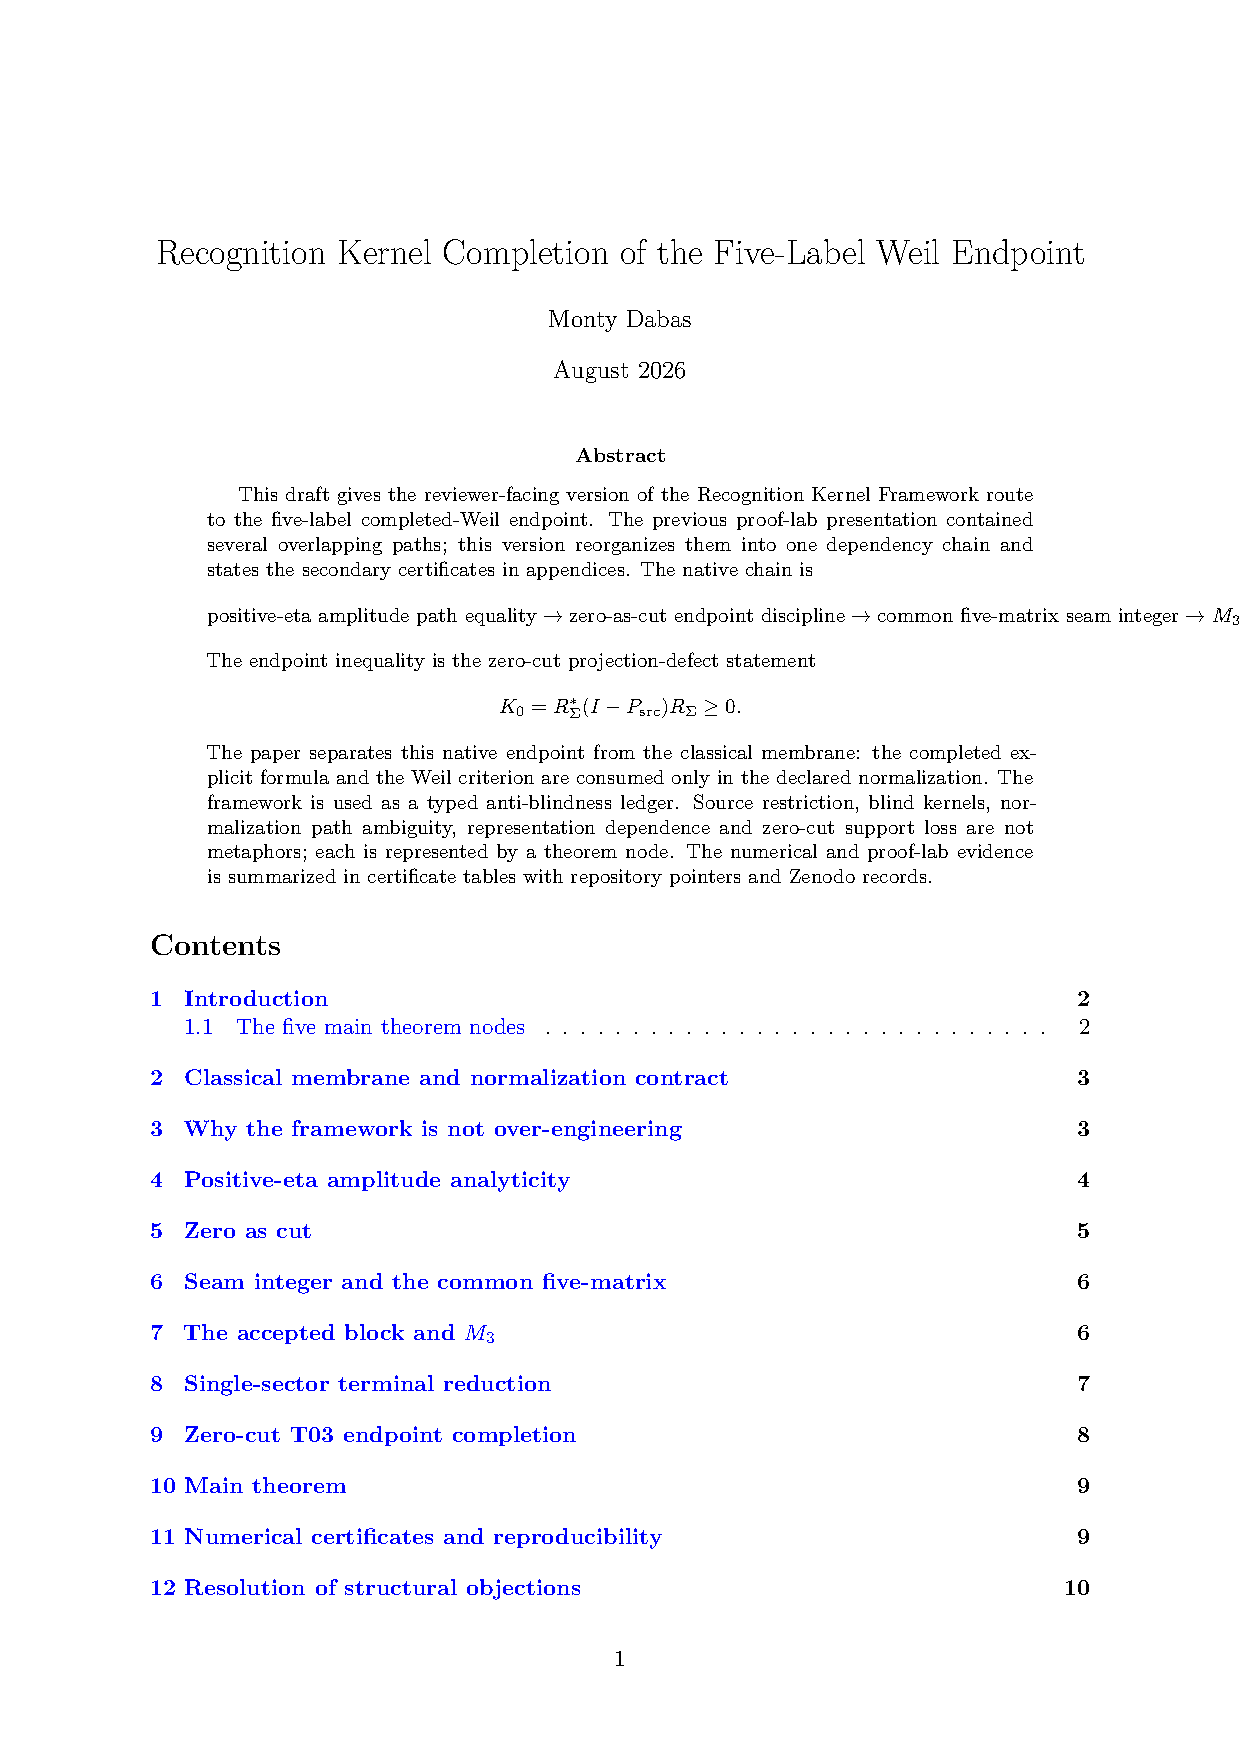
\includepdf[pages=-]{fragments/p085.pdf}

\part{The RH-Framework Ladder}
% source: RH-Framework/README.md
\hypertarget{rh-framework-reviewer-verification-laboratory}{%
\chapter{RH Framework Reviewer Verification Laboratory}\label{rh-framework-reviewer-verification-laboratory}}

This private repository is the authoritative verification laboratory for the
Riemann-Hypothesis research programme.

It is separated from:

\begin{itemize}
\tightlist
\item
  \texttt{Parveen117/MP}, which preserves historical development and source lineage;
\item
  publication repositories, which contain manuscript-facing material;
\item
  public AI, ECL, cryptography and assurance repositories, which provide
  engineering patterns but are not mathematical proof dependencies.
\end{itemize}

\hypertarget{governing-rule}{%
\section{Governing rule}\label{governing-rule}}

\begin{verbatim}
proof statement
-> assumptions
-> foundational-origin label
-> executable witness
-> negative controls
-> immutable certificate
-> reviewer reproduction
-> promotion or rejection
\end{verbatim}

Theorem classifications are only:

\begin{verbatim}
PROVED
DISPROVED
OPEN
\end{verbatim}

Foundational origin is recorded separately. A theorem may be proved and still
be a classical import.

\hypertarget{active-branch}{%
\section{Active branch}\label{active-branch}}

\begin{verbatim}
agent/native-summability-reconstruction
\end{verbatim}

\hypertarget{native-reconstruction-now-proved}{%
\section{Native reconstruction now proved}\label{native-reconstruction-now-proved}}

\hypertarget{native-path-completion}{%
\subsection{Native path completion}\label{native-path-completion}}

\begin{verbatim}
T01-A  cut-tail path completion             PROVED
T01-B  recognition-Cauchy completion        PROVED
T01-C  completed native path action         PROVED
\end{verbatim}

The decisive native action estimate is

\[
\mathcal E_\Sigma(a\star\xi)
\le
\mathcal M_\Sigma(a)^2\mathcal E_\Sigma(\xi).
\]

It is derived from a finite weighted cut-square identity before ordinary
\(\ell^1\), \(\ell^2\), Hilbert space, or operator norm is introduced.

\begin{verbatim}
PASS_NATIVE_CUT_TAIL_AND_RECOGNITION_CAUCHY_COMPLETION_CORE
4e88898fc93010a6ba189f932817d0715298f106aff61528bb2e58acb8c6dbfd
\end{verbatim}

\hypertarget{native-refinement-content}{%
\subsection{Native refinement content}\label{native-refinement-content}}

\begin{verbatim}
T01-E1  reciprocal refinement content       PROVED
T01-E2  complete finite-content algebra      PROVED
T01-E3  native simple integrals              PROVED
\end{verbatim}

Cell content is reciprocal refinement count:

\[
\nu_R(c)=\frac1{n_sn_tn_\alpha}.
\]

Common refinement, finite additivity, symmetric-difference completion, and
translation invariance are proved before Haar or Lebesgue measure is named.

\begin{verbatim}
PASS_NATIVE_REFINEMENT_COUNT_CONTENT_AND_SIMPLE_INTEGRALS
1366eeb443efc661c614a3bf8e7b95b9500a10d40104a579d3e2ec438c51feb9
\end{verbatim}

\hypertarget{native-function-completion}{%
\subsection{Native function completion}\label{native-function-completion}}

\begin{verbatim}
T01-E4A  tail-integrable function completion        PROVED
T01-E4B  recognition-integrable completion          PROVED
T01-E4C  bounded native simple multipliers          PROVED
\end{verbatim}

The two native gauges are

\[
d_1(f,g)=\mathcal I_{\rm tail}(f-g),
\qquad
d_2(f,g)=\mathcal I_{\rm rec}(f-g).
\]

They are completed by Cauchy presentations before ordinary \(L^1/L^2\)
notation. Arbitrary tail-completed functions are not falsely declared
multiplicatively closed.

\begin{verbatim}
PASS_NATIVE_SIMPLE_FUNCTION_TAIL_AND_RECOGNITION_COMPLETION_CORE
ca4d3443e057adbaa0c94a285263d8d136465eaf970c7fef73df70196972cad9
\end{verbatim}

\hypertarget{native-mean-multiplier-bound}{%
\subsection{Native mean-multiplier bound}\label{native-mean-multiplier-bound}}

\begin{verbatim}
T01-E4D-A  exact mean split of a multiplier action   PROVED
T01-E4D-B  mean + oscillation x deviation bound      PROVED
T01-E4D-C  alternating-product gap (restated §4.1)    OPEN (vacuum half PROVED in Publications YM-31)
\end{verbatim}

\[
\mathcal I_{\rm rec}(hf)\le\langle N(h)\rangle\,\mathcal I_{\rm rec}(f)
+\operatorname{osc}N(h)\,\mathcal D_{\rm rec}(f).
\]

Sharper than T01-E4C on recognition-flat states (equality with the mean on
the vacuum); neither bound dominates in general.

\begin{verbatim}
PASS_NATIVE_MEAN_MULTIPLIER_IDENTITY_AND_BOUND
d6f3b39a0186a2c15c3fcd3734cf198ca6bd21b9182ad72906f0930341fe4c99
\end{verbatim}

\hypertarget{rational-normalized-ugd-refinement-adapter}{%
\subsection{Rational normalized-UGD refinement adapter}\label{rational-normalized-ugd-refinement-adapter}}

\begin{verbatim}
T01-E5A  rational native UGD linearization    PROVED
T01-E5B  rational refinement action           PROVED
\end{verbatim}

A rational normalized packet is

\[
N=(p,u,\mu),
\]

where \(p\) is a full-turn fraction, \(u\) is native scale debt, and \(\mu\)
is corrected seam memory. The exact map

\[
(p,u,\mu)\mapsto(u,p+\mu,[\mu])
\]

linearizes the wrap law and produces exact refinement-cell translations without
\(\pi\), \texttt{log}, \texttt{exp}, Haar measure, or floating point.

\begin{verbatim}
PASS_NATIVE_RATIONAL_UGD_REFINEMENT_LATTICE_ADAPTER
932d3e549e3a01d7d42d85e70371dc74fa06c214841bca8f776d19dd70ce4bc7
\end{verbatim}

\hypertarget{native-foundational-files}{%
\section{Native foundational files}\label{native-foundational-files}}

\begin{verbatim}
src/rh_framework/native_summability.py
src/rh_framework/native_refinement_measure.py
src/rh_framework/native_function_completion.py
src/rh_framework/native_ugd_refinement_adapter.py
\end{verbatim}

The verifier rejects approximate numerical identifiers and undeclared external
imports in these files.

\hypertarget{remaining-native-boundary}{%
\section{Remaining native boundary}\label{remaining-native-boundary}}

\begin{verbatim}
T01-E5C  complete the rational UGD group and action
T01-E6   actual positive-scale, log-exp, Haar and Jacobian shadows
T01-D    actual MP path-atlas and refinement adapter
T01-F    remaining classical coordinate identifications
native path-graph generator domains
native state-packet generation
representation invariance of FFT, Gram, spectral and polar charts
\end{verbatim}

The actual positive numerical scale \(\sigma\) has not been declared native.
The formal scale-debt ledger must be completed first; \(\sigma=e^u\) may appear
later only as a proved coordinate chart.

\hypertarget{classical-verification-shell}{%
\section{Classical verification shell}\label{classical-verification-shell}}

T03-A and T03-C2A remain rigorous, proved classical coordinate theorems. They
are not reclassified as native merely because native objects now exist beneath
them.

T03-B, T03-C1, and T03-C2B require pinned private MP worktrees and remain open.

\hypertarget{reproduction}{%
\section{Reproduction}\label{reproduction}}

\begin{verbatim}
python -m pip install -e .
python tools/verify_native_foundation.py
python tools/verify_t03.py
\end{verbatim}

Jupyter-only procedures are under \texttt{notebooks/}.

\hypertarget{claim-boundary}{%
\section{Claim boundary}\label{claim-boundary}}

The native abstract foundation has advanced substantially, but the actual MP
adapter, completed positive-scale UGD carrier, target faithfulness, Shunya,
critical-line equivalence, and the Riemann Hypothesis remain open.

\begin{flushright}\small\texttt{RH-Framework/README.md}\end{flushright}

% source: RH-Framework/REVIEWER_CHECKLIST.md
\hypertarget{reviewer-checklist}{%
\chapter{Reviewer Checklist}\label{reviewer-checklist}}

This repository separates theorem truth, foundational origin, executable evidence, and publication claims. Review them independently. Apparently one label was too convenient for civilization.

\hypertarget{scope}{%
\section{1. Scope}\label{scope}}

Confirm that the pull request changes only verification-facing material in \texttt{RH-Framework}. Historical MP development and manuscript sources must remain outside the diff.

\hypertarget{required-local-commands}{%
\section{2. Required local commands}\label{required-local-commands}}

\begin{verbatim}
python -m pip install -e .
python tools/check_text_integrity.py
python tools/verify_native_foundation.py
python tools/verify_t03.py
\end{verbatim}

The native verifier must reproduce all committed T01 certificates byte-for-byte. The T03 verifier must reproduce all source-independent classical-coordinate certificates.

\hypertarget{native-foundation-checks}{%
\section{3. Native-foundation checks}\label{native-foundation-checks}}

Confirm that foundational native modules:

\begin{itemize}
\tightlist
\item
  use exact rational arithmetic;
\item
  contain no executable \texttt{float}, \texttt{complex}, NumPy, SciPy, logarithm, exponential, or \texttt{pi} dependency;
\item
  derive cut-tail, recognition, refinement, function, and rational UGD structures before ordinary functional-analysis coordinates;
\item
  preserve explicit open boundaries for actual positive scale, MP adapters, state packets, target faithfulness, Shunya, and RH.
\end{itemize}

\hypertarget{classical-shell-checks}{%
\section{4. Classical-shell checks}\label{classical-shell-checks}}

Classical coordinate theorems may remain \texttt{PROVED}, but their origin must be \texttt{CLASSICAL\_THEOREM\_IMPORT} or \texttt{CLASSICAL\_NUMERICAL\_SOURCE} where applicable. They must not be described as foundational native derivations.

\hypertarget{certificates}{%
\section{5. Certificates}\label{certificates}}

For every committed certificate:

\begin{itemize}
\tightlist
\item
  regenerate it from source;
\item
  confirm deterministic canonical hashing;
\item
  inspect all false gates;
\item
  confirm theorem classifications use only \texttt{PROVED}, \texttt{DISPROVED}, or \texttt{OPEN};
\item
  confirm the certificate does not promote RH.
\end{itemize}

\hypertarget{private-source-gates}{%
\section{6. Private-source gates}\label{private-source-gates}}

T03-B, T03-C1, and T03-C2B require clean pinned MP worktrees. CI does not receive those worktrees, so absence of those results is an explicit open boundary rather than a CI failure.

\hypertarget{merge-decision}{%
\section{7. Merge decision}\label{merge-decision}}

Merge only when:

\begin{verbatim}
all required CI jobs pass;
committed certificates reproduce;
no theorem classification drifts;
foundational-origin labels are accurate;
no private-source claim is promoted without evidence;
open obligations are listed explicitly.
\end{verbatim}

\begin{flushright}\small\texttt{RH-Framework/REVIEWER\_CHECKLIST.md}\end{flushright}

% source: RH-Framework/theorems/LEDGER.md
\hypertarget{rh-framework-theorem-ledger}{%
\chapter{RH Framework Theorem Ledger}\label{rh-framework-theorem-ledger}}

Only \texttt{PROVED}, \texttt{DISPROVED}, and \texttt{OPEN} are theorem classifications.
Certificates, numerical passes, source availability, and foundational origin are
evidence fields rather than substitute theorem states.

Foundational origin is audited separately in
\texttt{NATIVE\_DERIVATION\_CONTAMINATION\_AUDIT.md} and the latest immutable manifest in
\texttt{provenance/}.

\hypertarget{t01-native-operator-algebra-and-recognition-completion}{%
\section{T01 --- Native operator algebra and recognition completion}\label{t01-native-operator-algebra-and-recognition-completion}}

\textbf{Classification:} \texttt{OPEN}

The abstract countable completion, refinement-content algebra, native function
completions, and rational normalized-UGD refinement action are constructed
inside RH-Framework. T01 remains open because the rational native scale-debt
carrier is not yet completed and identified with the actual positive UGD scale
or the actual MP path atlas.

\hypertarget{t01-a-native-cut-tail-completion}{%
\subsection{T01-A --- native cut-tail completion}\label{t01-a-native-cut-tail-completion}}

\textbf{Classification:} \texttt{PROVED}

For finite typed residue paths over exact cut scalars,

\[
\mathcal M_\Sigma(a)
=
\sum_\gamma
\bigl(|\operatorname{rad}a_\gamma|_\Sigma
+|\operatorname{turn}a_\gamma|_\Sigma\bigr).
\]

Cut-tail Cauchy presentations modulo cut-tail-null presentations form a complete
involutive path algebra without assuming ordinary complex numbers, \(\ell^1\),
Banach space, operator norm, Haar measure, or spectral theory.

\hypertarget{t01-b-native-recognition-cauchy-completion}{%
\subsection{T01-B --- native recognition-Cauchy completion}\label{t01-b-native-recognition-cauchy-completion}}

\textbf{Classification:} \texttt{PROVED}

The closed-loop energy

\[
\mathcal E_\Sigma(a)
=
\Phi_\Sigma(a^\dagger\star a)
=
\sum_\gamma a_\gamma^\dagger a_\gamma
\]

defines a second Cauchy relation and a complete positive cut module with a
positive-definite completed pairing.

\hypertarget{t01-c-native-completed-path-action}{%
\subsection{T01-C --- native completed path action}\label{t01-c-native-completed-path-action}}

\textbf{Classification:} \texttt{PROVED}

The exact weighted cut-square identity gives

\[
\boxed{
\mathcal E_\Sigma(a\star\xi)
\le
\mathcal M_\Sigma(a)^2\mathcal E_\Sigma(\xi).
}
\]

Thus the cut-tail completion acts continuously on the recognition completion
without importing Cauchy-Schwarz, Young, Minkowski, Hilbert space, or an operator
norm as primitive theorems.

Proof:
\texttt{T01\_NATIVE\_SUMMABILITY\_AND\_RECOGNITION\_COMPLETION.md}.

\begin{verbatim}
PASS_NATIVE_CUT_TAIL_AND_RECOGNITION_CAUCHY_COMPLETION_CORE
4e88898fc93010a6ba189f932817d0715298f106aff61528bb2e58acb8c6dbfd
\end{verbatim}

\hypertarget{t01-d-actual-mp-path-atlas-adapter}{%
\subsection{T01-D --- actual MP path-atlas adapter}\label{t01-d-actual-mp-path-atlas-adapter}}

\textbf{Classification:} \texttt{OPEN}

Prove that actual source, response, prime, Gamma, boundary, continuation, and
seam paths embed into the native finite-support core and that actual refinement
maps are continuous for \(\mathcal M_\Sigma\) and \(\mathcal E_\Sigma\).

\hypertarget{t01-e-native-refinement-and-ugd-programme}{%
\subsection{T01-E --- native refinement and UGD programme}\label{t01-e-native-refinement-and-ugd-programme}}

\textbf{Classification:} \texttt{OPEN}

The abstract content, function, and rational UGD refinement theorems are proved.
The completed actual positive-scale carrier and its state-locked adapter remain
open.

\hypertarget{t01-e1-native-refinement-count-content}{%
\subsubsection{T01-E1 --- native refinement-count content}\label{t01-e1-native-refinement-count-content}}

\textbf{Classification:} \texttt{PROVED}

On a grid \(R=(n_s,n_t,n_\alpha)\), one cell has content

\[
\nu_R(c)=\frac{1}{n_sn_tn_\alpha}.
\]

Finite cylinders have reciprocal-cell-count content. Common refinement, finite
additivity, Boolean identities, and integer cell-translation invariance are
proved before any Haar or Lebesgue measure is introduced.

\hypertarget{t01-e2-complete-native-content-algebra}{%
\subsubsection{T01-E2 --- complete native content algebra}\label{t01-e2-complete-native-content-algebra}}

\textbf{Classification:} \texttt{PROVED}

The gauge

\[
\delta(A,B)=\nu(A\triangle B)
\]

defines refinement-content Cauchy presentations. Their quotient is a complete
finite-content algebra with extended nonnegative, finitely additive,
translation-invariant content.

No sigma-additivity theorem for arbitrary completed families is claimed.

\hypertarget{t01-e3-native-simple-tail-and-recognition-integrals}{%
\subsubsection{T01-E3 --- native simple tail and recognition integrals}\label{t01-e3-native-simple-tail-and-recognition-integrals}}

\textbf{Classification:} \texttt{PROVED}

For finite cut-scalar simple functions,

\[
\mathcal I_{\rm tail}(f)
=
\sum_c\nu_R(c)D_\Sigma(f(c)),
\qquad
\mathcal I_{\rm rec}(f)
=
\sum_c\nu_R(c)N_\Sigma(f(c)).
\]

Both are invariant under native refinement and integer cell translation.

Proof:
\texttt{T01\_E\_NATIVE\_REFINEMENT\_COUNT\_MEASURE.md}.

\begin{verbatim}
PASS_NATIVE_REFINEMENT_COUNT_CONTENT_AND_SIMPLE_INTEGRALS
1366eeb443efc661c614a3bf8e7b95b9500a10d40104a579d3e2ec438c51feb9
\end{verbatim}

\hypertarget{t01-e4a-native-tail-integrable-function-completion}{%
\subsubsection{T01-E4A --- native tail-integrable function completion}\label{t01-e4a-native-tail-integrable-function-completion}}

\textbf{Classification:} \texttt{PROVED}

Finite simple functions completed under

\[
d_1(f,g)=\mathcal I_{\rm tail}(f-g)
\]

form a complete native cut module. Ordinary \(L^1\) is not used as definition.

\hypertarget{t01-e4b-native-recognition-integrable-function-completion}{%
\subsubsection{T01-E4B --- native recognition-integrable function completion}\label{t01-e4b-native-recognition-integrable-function-completion}}

\textbf{Classification:} \texttt{PROVED}

Finite simple functions completed under

\[
d_2(f,g)=\mathcal I_{\rm rec}(f-g)
\]

form a complete positive cut module. The native pairing is extended using a
finite cut-square identity before any Hilbert or ordinary \(L^2\) structure is
named.

\hypertarget{t01-e4c-native-bounded-simple-multipliers}{%
\subsubsection{T01-E4C --- native bounded simple multipliers}\label{t01-e4c-native-bounded-simple-multipliers}}

\textbf{Classification:} \texttt{PROVED}

For a bounded native simple multiplier \(h\),

\[
\mathcal I_{\rm tail}(hf)
\le U_\Sigma(h)\mathcal I_{\rm tail}(f),
\]

\[
\mathcal I_{\rm rec}(hf)
\le U_\Sigma(h)^2\mathcal I_{\rm rec}(f).
\]

No multiplicative closure is claimed for arbitrary tail-completed functions.

Proof:
\texttt{T01\_E4\_NATIVE\_FUNCTION\_COMPLETION.md}.

\begin{verbatim}
PASS_NATIVE_SIMPLE_FUNCTION_TAIL_AND_RECOGNITION_COMPLETION_CORE
ca4d3443e057adbaa0c94a285263d8d136465eaf970c7fef73df70196972cad9
\end{verbatim}

\hypertarget{t01-e4d-native-mean-multiplier-identity-and-bound}{%
\subsubsection{T01-E4D --- native mean-multiplier identity and bound}\label{t01-e4d-native-mean-multiplier-identity-and-bound}}

\textbf{Classification:} \texttt{PROVED}

Exact mean split on the unit box,

\[
\mathcal I_{\rm rec}(hf)
=
\langle N(h)\rangle\,\mathcal I_{\rm rec}(f)
+\operatorname{Cov}_\nu\bigl(N(h),N(f)\bigr),
\]

and the bound

\[
\mathcal I_{\rm rec}(hf)
\le
\langle N(h)\rangle\,\mathcal I_{\rm rec}(f)
+\operatorname{osc}N(h)\,\mathcal D_{\rm rec}(f),
\qquad
0\le\mathcal D_{\rm rec}(f)\le\mathcal I_{\rm rec}(f).
\]

A multiplier acts on a recognition-flat state by its mean, not its maximum.
T01-E4D-C is \texttt{OPEN} in its \textbf{corrected} form (theorem file §4.1): the
multiplier iterated on a fixed state converges to its supremum, not its mean
(certified, Publications YM-34), so the item is restated as the \(m\)-uniform
gap of the alternating product \((K^{1/2}M_wK^{1/2})\); its vacuum half is
PROVED (Publications YM-31), its excitation half is the chain adapters'
remaining obligation (theorum/28 hypothesis 3).

\textbf{Status update (Aug 23 2026).} The excitation half has been reduced,
not closed. On the one-column transfer: the \(m\)-direction is
eliminated (Publications YM-37/YM-38 --- every quantity is one column, and
the uniformity argument is native: T53 elimination + theorum/28 §9
outward certificate, no spectral decomposition); the content direction is
released lawfully with exact seam-count retention (RKF theorum/75, native
character-ladder regrading); the contraction itself is structural rather
than Krylov (RKF theorum/74, silence channel). Dock and re-verification:
Publications YM-41. \textbf{What remains open of T01-E4D-C is the
\(t\)-direction only} --- whether the extracted gap persists uniformly in
the number of time rails --- together with the standing caveat that all of
this lives on the compressed column carrier (lower-bound side), not on
an operator upper bound for the chain. Named next: Publications YM-42.

Proof:
\texttt{T01\_E4D\_NATIVE\_MEAN\_MULTIPLIER\_BOUND.md}.

\begin{verbatim}
PASS_NATIVE_MEAN_MULTIPLIER_IDENTITY_AND_BOUND
d6f3b39a0186a2c15c3fcd3734cf198ca6bd21b9182ad72906f0930341fe4c99
\end{verbatim}

\hypertarget{t01-e5a-rational-native-ugd-group-linearization}{%
\subsubsection{T01-E5A --- rational native UGD group linearization}\label{t01-e5a-rational-native-ugd-group-linearization}}

\textbf{Classification:} \texttt{PROVED}

A rational normalized UGD packet is

\[
N=(p,u,\mu),
\]

where \(p\) is a full-turn rational phase, \(u\) is a native additive
scale-debt ledger, and \(\mu\) is corrected rational seam memory. Its product is

\[
(p,u,\mu)\star(q,v,\nu)
=
((p+q)^\flat,u+v,\mu+\nu+W(p,q)).
\]

The exact map

\[
\Psi_\Sigma(p,u,\mu)
=(u,p+\mu,[\mu])
\]

is a group isomorphism to

\[
\mathbb Q_\Sigma\times\mathbb Q_\Sigma
\times(\mathbb Q_\Sigma/\mathbb Z).
\]

No \(\pi\), logarithm, exponential, or positive-real scale is primitive.

\hypertarget{t01-e5b-rational-ugd-refinement-action}{%
\subsubsection{T01-E5B --- rational UGD refinement action}\label{t01-e5b-rational-ugd-refinement-action}}

\textbf{Classification:} \texttt{PROVED}

Compatible rational lifted points act as exact integer shifts of native
refinement cells. The action is covariant under refinement, preserves content,
and converts UGD product into successive cell translation.

Proof:
\texttt{T01\_E5\_NATIVE\_RATIONAL\_UGD\_REFINEMENT\_ADAPTER.md}.

\begin{verbatim}
PASS_NATIVE_RATIONAL_UGD_REFINEMENT_LATTICE_ADAPTER
932d3e549e3a01d7d42d85e70371dc74fa06c214841bca8f776d19dd70ce4bc7
\end{verbatim}

\hypertarget{t01-e5c-completed-actual-ugd-adapter}{%
\subsubsection{T01-E5C --- completed actual UGD adapter}\label{t01-e5c-completed-actual-ugd-adapter}}

\textbf{Classification:} \texttt{OPEN}

Complete the rational phase, scale-debt, and memory group; extend the refinement
action to all completed points; identify the actual state-locked UGD packet with
that completion; and prove that the actual positive scale is a coordinate shadow
rather than the definition of scale debt.

\hypertarget{t01-e6-positive-scale-haar-jacobian-and-ordinary-lp-shadows}{%
\subsubsection{T01-E6 --- positive-scale, Haar, Jacobian, and ordinary Lp shadows}\label{t01-e6-positive-scale-haar-jacobian-and-ordinary-lp-shadows}}

\textbf{Classification:} \texttt{OPEN}

Only after T01-E5C may \(\sigma=e^u\), flat Haar coordinates, the
\(\sigma^{-2}\) density, and ordinary \(L^1/L^2\) models be proved as coordinate
shadows of the native objects.

\hypertarget{t01-f-remaining-coordinate-shadow-identifications}{%
\subsection{T01-F --- remaining coordinate-shadow identifications}\label{t01-f-remaining-coordinate-shadow-identifications}}

\textbf{Classification:} \texttt{OPEN}

Prove equivalences with ordinary sequence-space, Hilbert,
regular-representation, and continuous group models after native construction.

\hypertarget{t02-state-locked-five-label-carrier-realization}{%
\section{T02 --- State-locked five-label carrier realization}\label{t02-state-locked-five-label-carrier-realization}}

\textbf{Classification:} \texttt{OPEN}

A provenance-controlled interface exists in the pinned MP source. RH-Framework
must reproduce it from immutable worktrees and store its certificate before T02
can be classified.

\begin{verbatim}
PASS_STATE_LOCKED_CUT_APERTURE_CARRIER_INTERFACE
\end{verbatim}

\hypertarget{t03-actual-action-domain-adapter}{%
\section{T03 --- Actual action-domain adapter}\label{t03-actual-action-domain-adapter}}

\textbf{Classification:} \texttt{OPEN}

\hypertarget{t03-a-classical-normalized-ugd-action-domain-theorem}{%
\subsection{T03-A --- classical normalized-UGD action-domain theorem}\label{t03-a-classical-normalized-ugd-action-domain-theorem}}

\textbf{Classification:} \texttt{PROVED}

On the classical coordinate carrier

\[
\mathcal H=L^2(\mathbb R_u\times\mathbb R_t\times S^1_\alpha;\mathbb C^5),
\]

bounded multiplier, convolution, and maximal multiplication-operator theorems
are proved. Foundational origin is \texttt{CLASSICAL\_THEOREM\_IMPORT}; T03-A is not the
native construction supplied by T01.

\begin{verbatim}
PASS_T03_ACTION_DOMAIN_DENSE_CORE
05a4784308e996763928b4cead0c86462150154c506b30bf292f96dd8986db3c
\end{verbatim}

\hypertarget{t03-b-finite-state-locked-packet-reproduction}{%
\subsection{T03-B --- finite state-locked packet reproduction}\label{t03-b-finite-state-locked-packet-reproduction}}

\textbf{Classification:} \texttt{OPEN}

The reproducer verifies exact clean MP worktrees and rejects changed source
blobs, false checks, wrong labels, or dirty checkouts.

\hypertarget{t03-c1-actual-finite-packet-action-inventory}{%
\subsection{T03-C1 --- actual finite packet action inventory}\label{t03-c1-actual-finite-packet-action-inventory}}

\textbf{Classification:} \texttt{OPEN}

The finite-action typing theorem and pinned extractor are implemented. The
actual private packet has not yet been executed inside RH-Framework.

\begin{verbatim}
PASS_RH_FRAMEWORK_T03_C1_PINNED_ACTION_INVENTORY
\end{verbatim}

A passing run promotes T03-B and T03-C1 together.

\hypertarget{t03-c2a-positive-eta-family-envelope-theorem}{%
\subsection{T03-C2A --- positive-eta family envelope theorem}\label{t03-c2a-positive-eta-family-envelope-theorem}}

\textbf{Classification:} \texttt{PROVED}

The source-independent theorem correctly types amplitudes as analysis maps and
proves compact-positive-eta bounds. Its origin is
\texttt{CLASSICAL\_THEOREM\_IMPORT} because it uses complex polar and spectral theory.

\begin{verbatim}
PASS_T03_C2A_POSITIVE_ETA_FAMILY_ENVELOPE
d64d8b02...c6e8
\end{verbatim}

\hypertarget{t03-c2b-actual-pinned-positive-eta-family}{%
\subsection{T03-C2B --- actual pinned positive-eta family}\label{t03-c2b-actual-pinned-positive-eta-family}}

\textbf{Classification:} \texttt{OPEN}

Execute the actual pinned MP eta family and bind its arrays and source blobs to
the T03-C2A hypotheses.

\hypertarget{t03-c3-arithmetic-gamma-boundary-and-compatibility-actions}{%
\subsection{T03-C3 --- arithmetic, Gamma, boundary, and compatibility actions}\label{t03-c3-arithmetic-gamma-boundary-and-compatibility-actions}}

\textbf{Classification:} \texttt{OPEN}

Each actual action must receive a native T01-domain statement and, when useful,
a classical T03 coordinate classification.

\hypertarget{t03-c4-unbounded-generator-graph-domains}{%
\subsection{T03-C4 --- unbounded generator graph domains}\label{t03-c4-unbounded-generator-graph-domains}}

\textbf{Classification:} \texttt{OPEN}

Derive native path-graph convergence first, then recover classical maximal or
closed graph domains as coordinate shadows.

\hypertarget{t03-c5-aperture-exhaustion}{%
\subsection{T03-C5 --- aperture exhaustion}\label{t03-c5-aperture-exhaustion}}

\textbf{Classification:} \texttt{OPEN}

Prove native refinement convergence before operator-topology or graph-norm
promotion.

\hypertarget{t04-target-faithfulness-and-residue-retention}{%
\section{T04 --- Target faithfulness and residue retention}\label{t04-target-faithfulness-and-residue-retention}}

\textbf{Classification:} \texttt{OPEN}

The native regular action is faithful on its abstract path core. The actual RH
target may still quotient nonzero seam residue; its kernel is not proved trivial
or completely identified.

\hypertarget{t05-native-shunya-exclusion}{%
\section{T05 --- Native Shunya exclusion}\label{t05-native-shunya-exclusion}}

\textbf{Classification:} \texttt{OPEN}

The formal positive square is identified, but the recognized-zero condition on
the actual native completed representation is not proved.

\hypertarget{t06-critical-line-adapter-and-completed-weil-equivalence}{%
\section{T06 --- Critical-line adapter and completed-Weil equivalence}\label{t06-critical-line-adapter-and-completed-weil-equivalence}}

\textbf{Classification:} \texttt{OPEN}

No theorem in RH-Framework proves completed-Weil positivity, global seam-charge
vanishing, odd/even continuum no-crossing, or the Riemann Hypothesis.

\hypertarget{native-reconstruction-order}{%
\section{Native reconstruction order}\label{native-reconstruction-order}}

\begin{verbatim}
T01-E5C completed actual UGD adapter
-> T01-E6 positive-scale/Haar/Jacobian/Lp coordinate shadows
-> T01-D actual MP path-atlas adapter
-> T01-F remaining coordinate identifications
-> native generator graph convergence
-> native state-packet generation
\end{verbatim}

\hypertarget{rh-verification-order}{%
\section{RH verification order}\label{rh-verification-order}}

\begin{verbatim}
pinned T03-C1 run, which also verifies T03-B
-> T03-C2B actual positive-eta family
-> T03-C3 arithmetic and Gamma actions
-> T03-C4 generator domains
-> T03-C5 aperture exhaustion
-> T04 target-kernel audit
-> T05 native Shunya
-> T06 critical-line equivalence
\end{verbatim}

\hypertarget{global-claim}{%
\section{Global claim}\label{global-claim}}

\textbf{Riemann Hypothesis:} \texttt{OPEN}

\begin{flushright}\small\texttt{RH-Framework/theorems/LEDGER.md}\end{flushright}

% source: RH-Framework/theorems/NATIVE_DERIVATION_CONTAMINATION_AUDIT.md
\hypertarget{native-derivation-and-classical-import-audit}{%
\chapter{Native Derivation and Classical-Import Audit}\label{native-derivation-and-classical-import-audit}}

\hypertarget{current-verdict}{%
\section{Current verdict}\label{current-verdict}}

The RH framework remains \textbf{mixed}, not purely native.

The native boundary has moved substantially. RH-Framework now constructs, before
ordinary functional analysis:

\begin{verbatim}
cut-tail path completion;
recognition-Cauchy completion;
completed native path action;
refinement-count content;
complete finite-content algebra;
native tail and recognition simple integrals;
native completed function modules;
native bounded simple multipliers;
rational normalized-UGD group and refinement action.
\end{verbatim}

The unresolved classical boundary now begins at completion of the actual
positive-scale UGD carrier, its Haar/Jacobian shadows, actual MP coefficient
adapters, generator domains, and numerical state-packet generation.

The origin vocabulary remains:

\begin{verbatim}
NATIVE_DERIVED
NATIVE_DERIVED_WITH_CLASSICAL_PROOF_TECHNIQUES
COORDINATE_SHADOW
CLASSICAL_THEOREM_IMPORT
CLASSICAL_NUMERICAL_SOURCE
OPEN_NATIVE_RECONSTRUCTION
\end{verbatim}

The theorem ledger and origin ledger answer different questions. A theorem can
be \texttt{PROVED} while still being a classical import.

\begin{center}\rule{0.5\linewidth}{0.5pt}\end{center}

\hypertarget{audit-standard}{%
\section{1. Audit standard}\label{audit-standard}}

Strong purity would forbid integers, rationals, finite sets, sequences,
equivalence relations, and ordinary logic. That is not claimed.

The active research standard is:

\begin{verbatim}
Do not assume ordinary complex numbers, L-p spaces, Hilbert space, operator
norms, spectral theory, positive-real UGD coordinates, or Haar measure before
deriving the native cut, path, dagger, positivity, summability, recognition,
refinement, function, and group structures that those classical objects are
meant to coordinate.
\end{verbatim}

\begin{center}\rule{0.5\linewidth}{0.5pt}\end{center}

\hypertarget{native-derived-layers}{%
\section{2. Native-derived layers}\label{native-derived-layers}}

\hypertarget{cut-arithmetic-and-finite-path-algebra}{%
\subsection{2.1 Cut arithmetic and finite path algebra}\label{cut-arithmetic-and-finite-path-algebra}}

\textbf{Origin:} \texttt{NATIVE\_DERIVED}

Signed cut counts, refinement classes, the radial/tangential cut plane,
quarter-turn multiplication, dagger, the finite positive cone, typed residue
paths, closed-loop positivity, seam bridges, cut-curvature squares, and residue
retention are constructed before ordinary complex coordinates.

\hypertarget{cut-scalar-completion}{%
\subsection{2.2 Cut-scalar completion}\label{cut-scalar-completion}}

\textbf{Origin:} \texttt{NATIVE\_DERIVED\_WITH\_CLASSICAL\_PROOF\_TECHNIQUES}

The completion object is ordered from cut-rational neighborhoods. Standard
sequence and diagonal meta-logic is used, but ordinary \(\mathbb C\) does not
generate the object.

The later map to ordinary complex numbers is a \texttt{COORDINATE\_SHADOW}.

\hypertarget{native-path-summability-and-recognition-completion}{%
\subsection{2.3 Native path summability and recognition completion}\label{native-path-summability-and-recognition-completion}}

\textbf{Origin:} \texttt{NATIVE\_DERIVED}

The foundational gauges are

\[
\mathcal M_\Sigma(a)
=
\sum_\gamma D_\Sigma(a_\gamma),
\]

\[
\mathcal E_\Sigma(a)
=
\Phi_\Sigma(a^\dagger\star a).
\]

Their Cauchy-presentation quotients are defined before \(\ell^1\), \(\ell^2\),
Banach space, Hilbert space, or operator norm. A weighted cut-square identity
proves

\[
\mathcal E_\Sigma(a\star\xi)
\le
\mathcal M_\Sigma(a)^2\mathcal E_\Sigma(\xi).
\]

The older MP \(\ell^1/\ell^2\) theorem is no longer foundational. Its proper
future role is a coordinate-shadow identification.

\hypertarget{native-refinement-count-content}{%
\subsection{2.4 Native refinement-count content}\label{native-refinement-count-content}}

\textbf{Origin:} \texttt{NATIVE\_DERIVED}

A refinement cell on grid \((n_s,n_t,n_\alpha)\) has content

\[
\frac1{n_sn_tn_\alpha}.
\]

Common refinement, finite additivity, symmetric-difference completion, and
integer cell-translation invariance are derived from exact cell counts. Haar,
Lebesgue, a Jacobian, and floating point are absent.

This gives a complete \textbf{finite-content algebra}, not an imported sigma-algebra.
No arbitrary countable-additivity claim has been smuggled into the vocabulary.

\hypertarget{native-function-completions}{%
\subsection{2.5 Native function completions}\label{native-function-completions}}

\textbf{Origin:} \texttt{NATIVE\_DERIVED}

Finite cut-scalar simple functions carry tail and recognition gauges

\[
\mathcal I_{\rm tail},
\qquad
\mathcal I_{\rm rec}.
\]

Their two Cauchy-presentation completions, the completed native pairing, and
bounded simple-multiplier estimates are proved before ordinary \(L^1\),
\(L^2\), Hilbert space, or decomposable operators are named.

Arbitrary tail-completed functions are not falsely declared multiplicatively
closed.

\hypertarget{rational-normalized-ugd-refinement-adapter}{%
\subsection{2.6 Rational normalized-UGD refinement adapter}\label{rational-normalized-ugd-refinement-adapter}}

\textbf{Origin:} \texttt{NATIVE\_DERIVED}

The rational normalized packet

\[
N=(p,u,\mu)
\]

uses:

\begin{verbatim}
p     full-turn rational phase;
u     additive native scale debt;
mu    corrected rational seam memory.
\end{verbatim}

The exact linearization

\[
(p,u,\mu)
\mapsto
(u,p+\mu,[\mu])
\]

proves the wrap law and rational refinement action without \(\pi\), logarithm,
exponential, positive-real scale, Haar measure, or a Jacobian.

Compatible rational packets act by exact content-preserving cell translations.

\begin{center}\rule{0.5\linewidth}{0.5pt}\end{center}

\hypertarget{classical-or-mixed-layers-still-present}{%
\section{3. Classical or mixed layers still present}\label{classical-or-mixed-layers-still-present}}

\hypertarget{actual-positive-ugd-scale}{%
\subsection{3.1 Actual positive UGD scale}\label{actual-positive-ugd-scale}}

\textbf{Origin:} \texttt{OPEN\_NATIVE\_RECONSTRUCTION}

The native scale-debt ledger \(u\) is not yet identified with an actual
numerical scale \(\sigma>0\).

The classical formula

\[
\sigma=e^u
\]

may later be a coordinate chart. It may not define native scale debt. Completion
of the rational native UGD group and binding of the state-locked packet remain
open.

\hypertarget{haar-and-original-coordinate-density}{%
\subsection{3.2 Haar and original-coordinate density}\label{haar-and-original-coordinate-density}}

\textbf{Origin:} \texttt{CLASSICAL\_THEOREM\_IMPORT\ /\ FUTURE\_COORDINATE\_SHADOW}

The previous continuous UGD theorem uses topological-group theory, Haar measure,
real logarithm/exponential, and a Jacobian to obtain

\[
d\lambda
\propto
\frac{d\phi\,d\sigma\,dk}{\sigma^2}.
\]

This remains useful, but it must be reproved after the completed native UGD
adapter as a coordinate-shadow theorem.

It is no longer allowed to generate the native refinement content or native
function completions.

\hypertarget{rh-framework-t03-a}{%
\subsection{3.3 RH-Framework T03-A}\label{rh-framework-t03-a}}

\textbf{Origin:} \texttt{CLASSICAL\_THEOREM\_IMPORT}

T03-A begins with

\[
L^2(\mathcal U_F;\mathbb C^5)
\]

and uses essential suprema, singular values, operator norms, Haar-translation
unitarity, Minkowski/Young bounds, resolvents, and maximal multiplication
operators. It is rigorous coordinate analysis, not the native foundation.

\hypertarget{state-locked-finite-packet}{%
\subsection{3.4 State-locked finite packet}\label{state-locked-finite-packet}}

\textbf{Origin:} \texttt{CLASSICAL\_NUMERICAL\_SOURCE\_WITH\_NATIVE\_REINTERPRETATION}

The packet is generated by complex arrays, FFT channels, Gram matrices,
eigendecomposition, singular values, polar frames, and numerical metric
transport.

The later exact cut embedding audits a native aperture relation but does not
retroactively make the source packet natively generated.

\hypertarget{positive-eta-family}{%
\subsection{3.5 Positive-eta family}\label{positive-eta-family}}

\textbf{Origin:} \texttt{CLASSICAL\_THEOREM\_IMPORT}

The typing correction is valid, but the theorem uses complex rectangular
amplitudes, polar decomposition, Hermitian Grams, spectral square roots, and
operator-norm continuity.

\begin{center}\rule{0.5\linewidth}{0.5pt}\end{center}

\hypertarget{foundational-source-boundary}{%
\section{4. Foundational source boundary}\label{foundational-source-boundary}}

The active native source files are:

\begin{verbatim}
src/rh_framework/native_summability.py
src/rh_framework/native_refinement_measure.py
src/rh_framework/native_function_completion.py
src/rh_framework/native_ugd_refinement_adapter.py
\end{verbatim}

They use exact rational arithmetic and internal native dependencies only. A
single verifier inspects their AST imports and rejects executable references to:

\begin{verbatim}
float;
complex;
numpy;
scipy;
log;
exp;
pi.
\end{verbatim}

The classical verification shell may use numerical libraries, but files in that
shell must not be cited as foundational native derivations.

\begin{center}\rule{0.5\linewidth}{0.5pt}\end{center}

\hypertarget{reconstruction-progress}{%
\section{5. Reconstruction progress}\label{reconstruction-progress}}

\begin{verbatim}
native cut-tail summability before ell1                 COMPLETE
native recognition completion before ell2               COMPLETE
native action bound before operator norm                 COMPLETE
native refinement content before Haar                    COMPLETE
native function completions before ordinary Lp           COMPLETE
rational normalized-UGD refinement law                  COMPLETE

completed actual positive-scale UGD adapter              OPEN
Haar/Jacobian/Lp coordinate-shadow theorem               OPEN
actual MP path-atlas adapter                             OPEN
native generator graph convergence                       OPEN
native state-packet generation                           OPEN
representation invariance of numerical charts            OPEN
actual target faithfulness                               OPEN
\end{verbatim}

\begin{center}\rule{0.5\linewidth}{0.5pt}\end{center}

\hypertarget{next-reconstruction-theorem}{%
\section{6. Next reconstruction theorem}\label{next-reconstruction-theorem}}

The next theorem must complete the rational native UGD group and extend its
refinement action to completed points. It must then bind the actual state-locked
UGD packet without defining scale debt by logarithm.

Only afterward may the classical log-exp/Haar theorem be admitted as a
coordinate shadow.

\begin{center}\rule{0.5\linewidth}{0.5pt}\end{center}

\hypertarget{current-audit-conclusion}{%
\section{7. Current audit conclusion}\label{current-audit-conclusion}}

\begin{verbatim}
EVERYTHING PURELY NATIVE                          NO
FINITE CUT/PATH ALGEBRA NATIVE                    YES
NATIVE COUNTABLE PATH COMPLETION                  YES
NATIVE REFINEMENT CONTENT                         YES
NATIVE FUNCTION COMPLETIONS                       YES
RATIONAL NATIVE UGD REFINEMENT ACTION             YES
ACTUAL POSITIVE-SCALE UGD CARRIER NATIVE          NO
HAAR/JACOBIAN/Lp CONTINUOUS MODEL NATIVE          NO
T03-A NATIVE                                      NO
STATE-LOCKED PACKET NATIVELY GENERATED            NO
FULLY NATIVE RH PROOF ESTABLISHED                 NO
\end{verbatim}

No RH claim may use the phrase \texttt{fully\ native\ proof} until the completed actual
UGD adapter, actual MP path/action adapters, generator, packet, target,
Shunya, and critical-line gates are closed.

\begin{flushright}\small\texttt{RH-Framework/theorems/NATIVE\_DERIVATION\_CONTAMINATION\_AUDIT.md}\end{flushright}

% source: RH-Framework/theorems/T01_E4D_NATIVE_MEAN_MULTIPLIER_BOUND.md
\hypertarget{t01-e4d-native-mean-multiplier-identity-and-bound}{%
\chapter{T01-E4D --- Native Mean-Multiplier Identity and Bound}\label{t01-e4d-native-mean-multiplier-identity-and-bound}}

\textbf{Classification:} \texttt{PROVED}

\textbf{Foundational origin:} \texttt{NATIVE\_DERIVED}

\textbf{Iterated-multiplier deviation control (T01-E4D-B):} \texttt{OPEN}

T01-E4C bounds a bounded native simple multiplier by its uniform cut bound
\(U_\Sigma(h)=\max_c D_\Sigma(h(c))\). That bound is tight only when the state
is concentrated where the multiplier is largest. This theorem proves the exact
finite identity that separates the \textbf{mean} action of a multiplier from its
\textbf{fluctuation}, and bounds the fluctuation by the multiplier's oscillation
times a native deviation of the state. Nothing beyond exact rational
arithmetic on refinement cells of one unit box is used.

\begin{center}\rule{0.5\linewidth}{0.5pt}\end{center}

\hypertarget{setting}{%
\section{1. Setting}\label{setting}}

Let \(R=(n_s,n_t,n_\alpha)\) be a refinement grid, \(B\) its unit box
(T01-E1, content \(\nu_R(B)=1\)), and let \(h,f\) be finite cut-scalar simple
functions supported in \(B\). Write \(N_\Sigma\) for the native norm square
(T01-B). Define on \(B\)

\[
\langle N(h)\rangle=\sum_{c\subset B}\nu_R(c)\,N_\Sigma(h(c))
=\mathcal I_{\rm rec}(h),
\qquad
\operatorname{osc}N(h)=\max_c N_\Sigma(h(c))-\min_c N_\Sigma(h(c)),
\]

and the \textbf{recognition deviation}

\[
\mathcal D_{\rm rec}(f)=\sum_{c\subset B}\nu_R(c)\,
\bigl(N_\Sigma(f(c))-\langle N(f)\rangle\bigr)_+ .
\tag{1.1}
\]

All three are refinement-invariant by T01-E3 (they are finite cell sums of
refinement-invariant simple integrals), and

\[
0\le\mathcal D_{\rm rec}(f)\le\mathcal I_{\rm rec}(f).
\tag{1.2}
\]

\begin{center}\rule{0.5\linewidth}{0.5pt}\end{center}

\hypertarget{theorem-e4d-a-exact-mean-split}{%
\section{2. Theorem E4D-A (exact mean split)}\label{theorem-e4d-a-exact-mean-split}}

\[
\boxed{
\mathcal I_{\rm rec}(hf)
=
\langle N(h)\rangle\,\mathcal I_{\rm rec}(f)
+
\sum_{c\subset B}\nu_R(c)
\bigl(N(h(c))-\langle N(h)\rangle\bigr)
\bigl(N(f(c))-\langle N(f)\rangle\bigr).
}
\tag{2.1}
\]

\hypertarget{proof}{%
\subsection{Proof}\label{proof}}

\(N_\Sigma\) is multiplicative on cut scalars (T01-B: \(N(ab)=N(a)N(b)\)), so
\(\mathcal I_{\rm rec}(hf)=\sum_c\nu(c)N(h(c))N(f(c))\). Expand
\(N(h(c))=\langle N(h)\rangle+(N(h(c))-\langle N(h)\rangle)\) and use
\(\sum_c\nu(c)(N(h(c))-\langle N(h)\rangle)=0\) on the unit box. QED.

\begin{center}\rule{0.5\linewidth}{0.5pt}\end{center}

\hypertarget{theorem-e4d-b-mean-multiplier-bound}{%
\section{3. Theorem E4D-B (mean-multiplier bound)}\label{theorem-e4d-b-mean-multiplier-bound}}

\[
\boxed{
\mathcal I_{\rm rec}(hf)
\le
\langle N(h)\rangle\,\mathcal I_{\rm rec}(f)
+
\operatorname{osc}N(h)\;\mathcal D_{\rm rec}(f).
}
\tag{3.1}
\]

\hypertarget{proof-1}{%
\subsection{Proof}\label{proof-1}}

Split the covariance sum of (2.1) into cells where
\(N(f(c))>\langle N(f)\rangle\) and cells where it is below. On the first set
the \(h\)-factor is at most \(\max N(h)-\langle N(h)\rangle\); on the second set
the \(h\)-factor is at least \(\min N(h)-\langle N(h)\rangle\) and multiplies a
negative quantity, so the contribution is at most
\((\langle N(h)\rangle-\min N(h))\sum_c\nu(c)(\langle N(f)\rangle-N(f(c)))_+\).
The positive and negative deviations of \(N(f)\) have equal content-weighted
mass on the unit box (their difference is \(\sum_c\nu(c)(N(f(c))-\langle N(f)\rangle)=0\)), so both sums equal \(\mathcal D_{\rm rec}(f)\). Adding the
two gaps gives \(\operatorname{osc}N(h)\). QED.

\hypertarget{corollaries}{%
\subsection{Corollaries}\label{corollaries}}

\begin{enumerate}
\def\labelenumi{\arabic{enumi}.}
\tightlist
\item
  \textbf{Vacuum equality.} If \(N(f)\) is constant on \(B\) then
  \(\mathcal D_{\rm rec}(f)=0\) and
  \(\mathcal I_{\rm rec}(hf)=\langle N(h)\rangle\,\mathcal I_{\rm rec}(f)\):
  a multiplier acts on a recognition-flat state by its \textbf{mean}, not its
  maximum.
\item
  \textbf{Product content.} If \(h_1\) depends only on the scale coordinate and
  \(h_2\) only on the seam coordinate then
  \(\langle N(h_1h_2)\rangle=\langle N(h_1)\rangle\langle N(h_2)\rangle\)
  (T01-E1 product content).
\item
  \textbf{Relation to T01-E4C.} Neither bound dominates: E4C is sharper for
  states concentrated at the multiplier's maximum, E4D is sharper for
  recognition-flat states. Both are lawful; the certificate records that
  E4D is strictly below E4C in all 40 pseudo-random trials.
\end{enumerate}

\begin{center}\rule{0.5\linewidth}{0.5pt}\end{center}

\hypertarget{what-is-not-claimed-t01-e4d-c-open}{%
\section{\texorpdfstring{4. What is not claimed (T01-E4D-C, \texttt{OPEN})}{4. What is not claimed (T01-E4D-C, OPEN)}}\label{what-is-not-claimed-t01-e4d-c-open}}

For an \textbf{iterated} product \(h_1h_2\cdots h_k f\) the bound (3.1) applies
face by face, but \(\mathcal D_{\rm rec}\) of the intermediate states is not
controlled by this theorem. Bounding the deviation along an iteration
uniformly in \(k\) is exactly the obligation that appears as hypothesis 3 of
the Recognition-Complete Finite-to-Infinite Cut Theorem
(Recognition-Kernel-Framework \texttt{theorum/28}) for the chain adapters
(Publications \texttt{yang-mills-certified-benchmark}, YM-26/27): there the
T01-E4C price per face is measured to exceed the true vacuum rate by factors
56.5 / 27.8 / 13.5, and Corollary 1 is the mechanism that removes the
maximum from the vacuum channel. No gap, no Haar shadow, and no RH statement
is promoted by this theorem.

\hypertarget{restatement-of-t01-e4d-c-aug-22-2026-after-publications-ym-34}{%
\subsection{4.1 Restatement of T01-E4D-C (Aug 22 2026, after Publications YM-34)}\label{restatement-of-t01-e4d-c-aug-22-2026-after-publications-ym-34}}

The obligation above is \textbf{not provable as written}. For a single face with
multiplier \(w=e^{\kappa\chi_{1/2}}\) the iterated ratio on one recognition
state,
\[
q_n=\frac{\int w^{\,n}}{\int w^{\,n-1}}=\frac{f_0(n\kappa)}{f_0((n-1)\kappa)},
\]
is strictly increasing and converges to \(\sup w=e^{2\kappa}\), not to the mean
\(f_0\) (certified for \(n\le 60\) at \(\kappa=1/8,1/4,1/2\): Publications
\texttt{ym34\_e4dc\_restated.py}, pin \texttt{EXPECTED\_YM34.sha256}). This is the native
Laplace principle: the mean law (3.1) holds once; iterated on a fixed state the
per-application price returns to the E4C supremum. Every exponential met in the
chain adapters (YM-16, YM-26 T2) is this growth.

With the recognition kernel \(K\) (content-\(j\) eigenvalue \(\lambda_j\)) applied
\textbf{between} multiplications the iterated ratio is nondecreasing (native
log-convexity, cut-square) and converges to
\(\lambda_1(K^{1/2}M_wK^{1/2})=f_0(1+\delta(\kappa))\) with
\(\delta=0.003582,\ 0.014032,\ 0.051911\), against a supremum price
\(e^{2\kappa}/f_0-1=0.274,\ 0.598,\ 1.405\). The smoothing step is what turns
the supremum into a spectral constant.

\textbf{T01-E4D-C (corrected statement, \texttt{OPEN}).} For the alternating product
\(S=(K^{1/2}M_wK^{1/2})\) on a chain of \(m\) faces,
\(\lambda_2(S)/\lambda_1(S)\le 1-\delta_{\rm gap}(\kappa)\) uniformly in \(m\).
The vacuum half (an \(m\)-uniform lower bound on \(\lambda_1\) at the true per-face
rate) is PROVED in Publications YM-31; the excitation half (an \(m\)-uniform upper
bound on \(\lambda_2\)) is the single open obligation, and any proof of it must
carry the smoothing step inside the iteration.

\begin{center}\rule{0.5\linewidth}{0.5pt}\end{center}

\hypertarget{certificate}{%
\section{5. Certificate}\label{certificate}}

\begin{verbatim}
src/rh_framework/native_mean_multiplier.py
src/rh_framework/native_mean_multiplier_certificate.py
certificates/T01_E4D_NATIVE_MEAN_MULTIPLIER_v0.1.json
tests/test_native_mean_multiplier.py
\end{verbatim}

Build note: the first draft of (3.1) used \(\max N(h)-\langle N(h)\rangle\)
in place of \(\operatorname{osc}N(h)\); the executable certificate refused it
(negative-side cells), and the proof above is the corrected statement.

\begin{flushright}\small\texttt{RH-Framework/theorems/T01\_E4D\_NATIVE\_MEAN\_MULTIPLIER\_BOUND.md}\end{flushright}

% source: RH-Framework/theorems/T01_E4_NATIVE_FUNCTION_COMPLETION.md
\hypertarget{t01-e4-native-simple-function-tail-and-recognition-completions}{%
\chapter{T01-E4 --- Native Simple-Function Tail and Recognition Completions}\label{t01-e4-native-simple-function-tail-and-recognition-completions}}

\textbf{Classification:} \texttt{PROVED}

\textbf{Foundational origin:} \texttt{NATIVE\_DERIVED}

\textbf{Actual UGD function adapter:} \texttt{OPEN}

This theorem completes finite cut-scalar simple functions using the native
refinement content of T01-E1/E2/E3. It does not begin with an ordinary
\(L^1\), \(L^2\), Hilbert, Haar, or Lebesgue structure.

\begin{center}\rule{0.5\linewidth}{0.5pt}\end{center}

\hypertarget{finite-native-simple-functions}{%
\section{1. Finite native simple functions}\label{finite-native-simple-functions}}

Let \(R=(n_s,n_t,n_\alpha)\) be a native refinement grid and let
\(C_R\) be its cell atlas. A finite native simple function is a finitely
supported map

\[
f:C_R\to\mathbb K_\Sigma^0.
\tag{1.1}
\]

If two functions live on different grids, refine both to the coordinatewise
least-common-multiple grid. Refinement copies each coarse value to all fine cells
inside that coarse cell.

Addition, subtraction, dagger, and pointwise multiplication are defined after
common refinement.

\begin{center}\rule{0.5\linewidth}{0.5pt}\end{center}

\hypertarget{native-integral-gauges}{%
\section{2. Native integral gauges}\label{native-integral-gauges}}

The tail integral is

\[
\boxed{
\mathcal I_1(f)
=
\sum_{c\in C_R}\nu_R(c)D_\Sigma(f(c)).
}
\tag{2.1}
\]

The recognition integral is

\[
\boxed{
\mathcal I_2(f)
=
\sum_{c\in C_R}\nu_R(c)N_\Sigma(f(c)).
}
\tag{2.2}
\]

T01-E3 proves that both values are unchanged by refinement and integer cell
translation.

Define

\[
d_1(f,g)=\mathcal I_1(f-g),
\tag{2.3}
\]

\[
d_2(f,g)=\mathcal I_2(f-g).
\tag{2.4}
\]

The second expression is an energy gauge rather than a square-root norm.

\begin{center}\rule{0.5\linewidth}{0.5pt}\end{center}

\hypertarget{tail-gauge-control}{%
\section{3. Tail-gauge control}\label{tail-gauge-control}}

For cut scalars,

\[
D_\Sigma(x+y)
\le D_\Sigma(x)+D_\Sigma(y).
\]

Summing over a common refinement gives

\[
\boxed{
d_1(f,h)\le d_1(f,g)+d_1(g,h).}
\tag{3.1}
\]

Thus \(d_1\) is a rational refinement-invariant distance on finite simple
functions modulo equality after common refinement.

A sequence \((f_n)\) is \textbf{tail Cauchy} when for every positive cut rational
\(\varepsilon\),

\[
d_1(f_m,f_n)<\varepsilon
\]

for all sufficiently large \(m,n\).

Define

\[
\boxed{
\mathfrak F_{\Sigma,1}
=
\{\text{tail-Cauchy simple presentations}\}/\sim_{d_1}.
}
\tag{3.2}
\]

\hypertarget{theorem-3.1}{%
\subsection{Theorem 3.1}\label{theorem-3.1}}

\(\mathfrak F_{\Sigma,1}\) is a complete cut module. Refinement and integer cell
translation extend as isometries.

\hypertarget{proof}{%
\subsection{Proof}\label{proof}}

Addition and scalar multiplication are uniformly continuous by the scalar tail
triangle inequality and

\[
\mathcal I_1(zf)
=D_\Sigma(z)\mathcal I_1(f).
\]

The Cauchy-presentation quotient is well defined. Completeness follows from the
diagonal presentation construction using only positive cut-rational thresholds.
Refinement and translation preserve \(\mathcal I_1\) on the finite core, hence
extend to the completion. QED.

This object is the \textbf{native tail-integrable function completion}. Ordinary
\(L^1\) is not its definition.

\begin{center}\rule{0.5\linewidth}{0.5pt}\end{center}

\hypertarget{recognition-gauge-control}{%
\section{4. Recognition-gauge control}\label{recognition-gauge-control}}

For cut scalars,

\[
2N_\Sigma(x)+2N_\Sigma(y)-N_\Sigma(x+y)
=N_\Sigma(x-y)\ge0.
\tag{4.1}
\]

After summation,

\[
\boxed{
\mathcal I_2(f+g)
\le
2\mathcal I_2(f)+2\mathcal I_2(g).
}
\tag{4.2}
\]

A sequence \((f_n)\) is \textbf{recognition Cauchy} when for every positive cut
rational \(\varepsilon\),

\[
d_2(f_m,f_n)<\varepsilon
\]

for all sufficiently large \(m,n\).

Define

\[
\boxed{
\mathfrak F_{\Sigma,2}
=
\{\text{recognition-Cauchy simple presentations}\}/\sim_{d_2}.
}
\tag{4.3}
\]

\begin{center}\rule{0.5\linewidth}{0.5pt}\end{center}

\hypertarget{native-completed-pairing}{%
\section{5. Native completed pairing}\label{native-completed-pairing}}

For finite simple functions, define

\[
\boxed{
\langle f,g\rangle_{\Sigma,\nu}^0
=
\sum_c\nu_R(c)f(c)^\dagger g(c),
}
\tag{5.1}
\]

after common refinement.

The exact finite cut-square identity gives

\[
\boxed{
N_\Sigma\left(
\langle f,g\rangle_{\Sigma,\nu}^0
\right)
\le
\mathcal I_2(f)\mathcal I_2(g).
}
\tag{5.2}
\]

One proof clears the rational cell denominators and applies the finite
coefficient identity

\[
\left(\sum_iN(x_i)\right)
\left(\sum_iN(y_i)\right)
-
N\left(\sum_i x_i^\dagger y_i\right)
=
\sum_{i<j}N(x_iy_j-x_jy_i).
\tag{5.3}
\]

No pre-existing inner-product theorem is used.

\hypertarget{theorem-5.1}{%
\subsection{Theorem 5.1}\label{theorem-5.1}}

The pairing extends uniquely to

\[
\langle\cdot,\cdot\rangle_{\Sigma,\nu}:
\mathfrak F_{\Sigma,2}\times
\mathfrak F_{\Sigma,2}
\to
\widehat{\mathbb K}_\Sigma.
\tag{5.4}
\]

It satisfies dagger symmetry, cut-linearity, positivity, and

\[
\langle f,f\rangle_{\Sigma,\nu}=0
\Longleftrightarrow f=0.
\tag{5.5}
\]

\hypertarget{proof-1}{%
\subsection{Proof}\label{proof-1}}

Recognition-Cauchy presentations are energy bounded. Apply \texttt{(5.2)} to pairing
differences exactly as in T01-B. Positivity and definiteness follow from
\(\mathcal I_2(f)\) and the recognition-null equivalence relation. QED.

Therefore \(\mathfrak F_{\Sigma,2}\) is the complete \textbf{native recognition-
integrable function module}. Hilbert space may appear later only as a coordinate
shadow.

\begin{center}\rule{0.5\linewidth}{0.5pt}\end{center}

\hypertarget{native-bounded-simple-multipliers}{%
\section{6. Native bounded simple multipliers}\label{native-bounded-simple-multipliers}}

For a finite simple function \(h\), define its uniform cut bound

\[
\boxed{
U_\Sigma(h)=\max_c D_\Sigma(h(c)).
}
\tag{6.1}
\]

Then pointwise multiplication obeys

\[
\boxed{
\mathcal I_1(hf)
\le U_\Sigma(h)\mathcal I_1(f),
}
\tag{6.2}
\]

and

\[
\boxed{
\mathcal I_2(hf)
\le U_\Sigma(h)^2\mathcal I_2(f).
}
\tag{6.3}
\]

\hypertarget{proof-2}{%
\subsection{Proof}\label{proof-2}}

For every cell,

\[
D_\Sigma(h(c)f(c))
\le D_\Sigma(h(c))D_\Sigma(f(c))
\le U_\Sigma(h)D_\Sigma(f(c)),
\]

while

\[
N_\Sigma(h(c)f(c))
=N_\Sigma(h(c))N_\Sigma(f(c))
\le U_\Sigma(h)^2N_\Sigma(f(c)).
\]

Multiply by cell content and sum. QED.

Thus every bounded native simple multiplier extends continuously to both native
function completions.

This theorem does \textbf{not} claim that the product of two arbitrary tail-completed
functions remains tail-integrable. Such closure requires a separate hypothesis.

\begin{center}\rule{0.5\linewidth}{0.5pt}\end{center}

\hypertarget{explicit-cauchy-function}{%
\section{7. Explicit Cauchy function}\label{explicit-cauchy-function}}

On the unit-denominator grid, define

\[
f_N
=
\sum_{n=0}^{N}
2^{-(n+1)}1_{c_n},
\tag{7.1}
\]

where the \(c_n\) are distinct native cells. Then for \(M>N\),

\[
d_1(f_M,f_N)
=
\sum_{n=N+1}^{M}2^{-(n+1)}
<2^{-(N+1)},
\tag{7.2}
\]

and

\[
d_2(f_M,f_N)
=
\sum_{n=N+1}^{M}4^{-(n+1)}
<\frac{1}{3\,4^{N+1}}.
\tag{7.3}
\]

The same presentation therefore defines elements in both native completions.

\begin{center}\rule{0.5\linewidth}{0.5pt}\end{center}

\hypertarget{foundational-exclusion-boundary}{%
\section{8. Foundational exclusion boundary}\label{foundational-exclusion-boundary}}

The theorem does not use as definitions or proof generators:

\begin{verbatim}
ordinary L1 or L2 spaces;
Hilbert space;
Haar or Lebesgue integration;
operator norms;
complex floating-point values;
spectral or polar decomposition.
\end{verbatim}

The implementation uses exact cut scalars and rational cell content only.

\begin{center}\rule{0.5\linewidth}{0.5pt}\end{center}

\hypertarget{coordinate-shadow-boundary}{%
\section{9. Coordinate-shadow boundary}\label{coordinate-shadow-boundary}}

After the actual UGD refinement adapter is proved, one may attempt to identify

\begin{verbatim}
native tail function completion         with an ordinary L1 chart;
native recognition function completion with an ordinary L2 chart;
native bounded multipliers              with decomposable bounded operators.
\end{verbatim}

Those must be equivalence theorems. They may not be used as definitions of the
native objects above.

\begin{center}\rule{0.5\linewidth}{0.5pt}\end{center}

\hypertarget{exact-certificate}{%
\section{10. Exact certificate}\label{exact-certificate}}

The expected status is

\begin{verbatim}
PASS_NATIVE_SIMPLE_FUNCTION_TAIL_AND_RECOGNITION_COMPLETION_CORE
\end{verbatim}

The exact certificate verifies cross-refinement arithmetic, pairing identities,
native multiplier bounds, a nontrivial Cauchy function, and the absence of
classical numerical dependencies in the foundational module.

\begin{center}\rule{0.5\linewidth}{0.5pt}\end{center}

\hypertarget{remaining-gates}{%
\section{11. Remaining gates}\label{remaining-gates}}

\begin{verbatim}
T01-E4A NATIVE TAIL FUNCTION COMPLETION           PROVED
T01-E4B NATIVE RECOGNITION FUNCTION COMPLETION    PROVED
T01-E4C NATIVE BOUNDED SIMPLE MULTIPLIERS          PROVED

T01-E5 ACTUAL UGD REFINEMENT ADAPTER               OPEN
T01-E6 HAAR AND ORDINARY L1/L2 SHADOWS             OPEN
ACTUAL MP ACTIONS ON NATIVE FUNCTION DOMAINS       OPEN
NATIVE STATE-PACKET GENERATION                     OPEN
TARGET FAITHFULNESS                                OPEN
NATIVE SHUNYA                                      OPEN
RIEMANN HYPOTHESIS                                 OPEN
\end{verbatim}

\begin{flushright}\small\texttt{RH-Framework/theorems/T01\_E4\_NATIVE\_FUNCTION\_COMPLETION.md}\end{flushright}

% source: RH-Framework/theorems/T01_E5_NATIVE_RATIONAL_UGD_REFINEMENT_ADAPTER.md
\hypertarget{t01-e5ab-native-rational-ugd-refinement-adapter}{%
\chapter{T01-E5A/B --- Native Rational UGD Refinement Adapter}\label{t01-e5ab-native-rational-ugd-refinement-adapter}}

\textbf{Classification:} \texttt{PROVED}

\textbf{Foundational origin:} \texttt{NATIVE\_DERIVED}

\textbf{Completed actual UGD adapter:} \texttt{OPEN}

This theorem derives the rational refinement law of normalized UGD without using
\(\pi\), logarithm, exponential, positive-real coordinates, Haar measure, or a
Jacobian.

The native scale variable below is a signed \textbf{scale-debt ledger}. It is not yet
identified with an actual positive numerical scale \(\sigma\). That later
identification is a separate completion and coordinate-shadow problem.

\begin{center}\rule{0.5\linewidth}{0.5pt}\end{center}

\hypertarget{native-normalized-ugd-packets}{%
\section{1. Native normalized UGD packets}\label{native-normalized-ugd-packets}}

Let

\[
p\in\mathbb Q_\Sigma/\mathbb Z
\]

be a full-turn phase fraction, represented in the principal interval
\([0,1)\). Let

\[
u\in\mathbb Q_\Sigma
\]

be a signed scale-debt coordinate, and let

\[
\mu\in\mathbb Q_\Sigma
\]

be corrected seam memory.

A rational normalized UGD packet is

\[
N=(p,u,\mu).
\tag{1.1}
\]

For principal phase representatives define

\[
W(p,q)=\lfloor p+q\rfloor\in\{0,1\},
\tag{1.2}
\]

\[
(p+q)^\flat=p+q-W(p,q).
\tag{1.3}
\]

The product is

\[
\boxed{
(p,u,\mu)\star(q,v,\nu)
=
\left(
(p+q)^\flat,
 u+v,
 \mu+\nu+W(p,q)
\right).
}
\tag{1.4}
\]

This is the full-turn form of the gauge-normalized UGD memory law. No angle in
radians is required.

\begin{center}\rule{0.5\linewidth}{0.5pt}\end{center}

\hypertarget{group-theorem}{%
\section{2. Group theorem}\label{group-theorem}}

\hypertarget{theorem-2.1}{%
\subsection{Theorem 2.1}\label{theorem-2.1}}

Equation \texttt{(1.4)} defines an abelian group. Its identity is

\[
(0,0,0),
\tag{2.1}
\]

and its inverse is

\[
\boxed{
(p,u,\mu)^{-1}
=
\left(
(-p)^\flat,
-u,
-\mu-W(p,(-p)^\flat)
\right).
}
\tag{2.2}
\]

\hypertarget{proof}{%
\subsection{Proof}\label{proof}}

The raw full-turn sum of three principal phases is independent of bracketing.
Both bracketings subtract exactly the integer part of \(p+q+r\). Hence

\[
W(p,q)+W((p+q)^\flat,r)
=
W(q,r)+W(p,(q+r)^\flat).
\tag{2.3}
\]

This proves associativity of phase and memory. Scale debt and the remaining
memory terms add associatively. Symmetry of the raw phase sum proves
commutativity.

For \texttt{(2.2)}, principal phases sum to zero after their unique wrap, scale debts
cancel, and the memory correction cancels that wrap. QED.

\begin{center}\rule{0.5\linewidth}{0.5pt}\end{center}

\hypertarget{native-lifted-coordinates}{%
\section{3. Native lifted coordinates}\label{native-lifted-coordinates}}

Define

\[
\boxed{
\Psi_\Sigma(p,u,\mu)
=
(u,t,\alpha),
\qquad
t=p+\mu,
\qquad
\alpha=[\mu]\in\mathbb Q_\Sigma/\mathbb Z.
}
\tag{3.1}
\]

\hypertarget{theorem-3.1-rational-native-linearization}{%
\subsection{Theorem 3.1 --- Rational native linearization}\label{theorem-3.1-rational-native-linearization}}

\(\Psi_\Sigma\) is a group isomorphism from \texttt{(1.4)} to

\[
\boxed{
\mathbb Q_\Sigma
\times
\mathbb Q_\Sigma
\times
(\mathbb Q_\Sigma/\mathbb Z)
}
\tag{3.2}
\]

with componentwise addition.

\hypertarget{proof-1}{%
\subsection{Proof}\label{proof-1}}

Let

\[
p_{12}=p+q-W(p,q),
\qquad
\mu_{12}=\mu+\nu+W(p,q).
\]

Then

\[
\begin{aligned}
t_{12}
&=p_{12}+\mu_{12}\\
&=p+\mu+q+\nu\\
&=t_1+t_2.
\end{aligned}
\tag{3.3}
\]

Also

\[
[\mu_{12}]=[\mu+\nu]
\tag{3.4}
\]

because the wrap is integral, and scale debts add.

For the inverse map, let \((u,t,\alpha)\) be given with the unique principal
representative \(0\le\alpha<1\). Put

\[
n=\lfloor t-\alpha\rfloor,
\qquad
\mu=\alpha+n,
\qquad
p=(t-\alpha)-n.
\tag{3.5}
\]

Then \(0\le p<1\), \([\mu]=\alpha\), and \(p+\mu=t\). This is the unique
preimage. QED.

The theorem needs neither \(2\pi\) nor a logarithm. Full turns, scale debt, and
memory are primitive cut-ledger coordinates.

\begin{center}\rule{0.5\linewidth}{0.5pt}\end{center}

\hypertarget{rational-refinement-lattices}{%
\section{4. Rational refinement lattices}\label{rational-refinement-lattices}}

For a refinement grid

\[
R=(n_s,n_t,n_\alpha),
\]

define the compatible rational lattice

\[
\boxed{
\Lambda_R
=
\frac1{n_s}\mathbb Z
\times
\frac1{n_t}\mathbb Z
\times
\left(
\frac1{n_\alpha}\mathbb Z/\mathbb Z
\right).
}
\tag{4.1}
\]

A native lifted point \((u,t,\alpha)\) is compatible with \(R\) exactly when

\[
n_su\in\mathbb Z,
\qquad
n_tt\in\mathbb Z,
\qquad
n_\alpha\alpha\in\mathbb Z.
\tag{4.2}
\]

Its cell shift is

\[
\boxed{
S_R(u,t,\alpha)
=
(n_su,n_tt,n_\alpha\alpha),
}
\tag{4.3}
\]

with the final component reduced modulo \(n_\alpha\).

\hypertarget{theorem-4.1-lattice-action}{%
\subsection{Theorem 4.1 --- Lattice action}\label{theorem-4.1-lattice-action}}

For compatible points \(x,y\in\Lambda_R\),

\[
S_R(x+y)=S_R(x)+S_R(y),
\tag{4.4}
\]

with circular reduction in the seam component.

Therefore compatible rational UGD packets act on native cylinders by exact cell
translation.

\hypertarget{proof-2}{%
\subsection{Proof}\label{proof-2}}

Multiply componentwise rational addition by the declared denominators. The
first two coordinates add in \(\mathbb Z\), while the seam coordinate adds in
\(\mathbb Z/n_\alpha\mathbb Z\). QED.

\begin{center}\rule{0.5\linewidth}{0.5pt}\end{center}

\hypertarget{refinement-covariance}{%
\section{5. Refinement covariance}\label{refinement-covariance}}

Let \(R'\) refine \(R\), with refinement factors

\[
q_s=\frac{n_s'}{n_s},
\quad
q_t=\frac{n_t'}{n_t},
\quad
q_\alpha=\frac{n_\alpha'}{n_\alpha}.
\]

For every point compatible with \(R\),

\[
\boxed{
S_{R'}(x)
=
(q_sS_R^s(x),q_tS_R^t(x),q_\alpha S_R^\alpha(x)),
}
\tag{5.1}
\]

with the final coordinate reduced modulo \(n_\alpha'\).

Thus translating first and refining afterward gives the same fine cells as
refining first and applying the fine-grid shift.

\begin{center}\rule{0.5\linewidth}{0.5pt}\end{center}

\hypertarget{content-preserving-ugd-translation}{%
\section{6. Content-preserving UGD translation}\label{content-preserving-ugd-translation}}

Let \(A\) be a finite native cylinder on grid \(R\), and let \(N\) be a rational
normalized UGD packet whose lifted point is compatible with \(R\). Define

\[
T_NA
=
T_{S_R(\Psi_\Sigma(N))}A.
\tag{6.1}
\]

\hypertarget{theorem-6.1}{%
\subsection{Theorem 6.1}\label{theorem-6.1}}

\[
\boxed{
\nu(T_NA)=\nu(A).
}
\tag{6.2}
\]

Moreover,

\[
T_{N_1}(T_{N_2}A)
=
T_{N_1\star N_2}A.
\tag{6.3}
\]

\hypertarget{proof-3}{%
\subsection{Proof}\label{proof-3}}

The first statement is T01-E1 translation invariance. For the second, use the
group homomorphism \texttt{(3.3)} and the lattice action \texttt{(4.4)}. QED.

The same translations preserve the native simple-function tail and recognition
integrals by finite reindexing.

\begin{center}\rule{0.5\linewidth}{0.5pt}\end{center}

\hypertarget{what-is-native-here}{%
\section{7. What is native here}\label{what-is-native-here}}

The construction uses only:

\begin{verbatim}
full-turn rational phase;
integer phase wrap;
additive rational scale debt;
rational corrected memory;
rational quotient by integers;
finite refinement denominators;
integer cell shifts;
reciprocal-count content.
\end{verbatim}

It does not use:

\begin{verbatim}
pi or radians;
logarithm or exponential;
a primitive positive-real scale line;
real-coordinate topology;
Haar measure;
Jacobian density;
floating-point arithmetic.
\end{verbatim}

\begin{center}\rule{0.5\linewidth}{0.5pt}\end{center}

\hypertarget{actual-scale-boundary}{%
\section{8. Actual-scale boundary}\label{actual-scale-boundary}}

This theorem does \textbf{not} yet identify the native scale debt \(u\) with an
actual UGD numerical scale \(\sigma>0\).

The classical formula

\[
\sigma=e^u
\]

may later be proved as a coordinate chart after the native scale-debt completion
is fixed. It may not be used as the definition of \(u\).

Likewise, the full completed UGD carrier requires completion of rational phase,
scale-debt, and memory presentations and proof that the actual state-locked UGD
packet lands in that completion.

\begin{center}\rule{0.5\linewidth}{0.5pt}\end{center}

\hypertarget{exact-certificate}{%
\section{9. Exact certificate}\label{exact-certificate}}

The expected status is

\begin{verbatim}
PASS_NATIVE_RATIONAL_UGD_REFINEMENT_LATTICE_ADAPTER
\end{verbatim}

The certificate checks exact wrap, product, inverse, linearization, round trip,
compatible and incompatible lattice points, refinement covariance,
content-preserving translation, and product/translation covariance.

\begin{center}\rule{0.5\linewidth}{0.5pt}\end{center}

\hypertarget{remaining-gates}{%
\section{10. Remaining gates}\label{remaining-gates}}

\begin{verbatim}
T01-E5A RATIONAL NATIVE UGD LINEARIZATION          PROVED
T01-E5B RATIONAL UGD REFINEMENT ACTION             PROVED

T01-E5C COMPLETED ACTUAL UGD ADAPTER               OPEN
T01-E6 POSITIVE-SCALE/LOG-EXP COORDINATE SHADOW    OPEN
T01-E6 HAAR/JACOBIAN/Lp COORDINATE SHADOW          OPEN
STATE-LOCKED UGD PACKET TO NATIVE COMPLETION       OPEN
TARGET FAITHFULNESS                                OPEN
NATIVE SHUNYA                                      OPEN
RIEMANN HYPOTHESIS                                 OPEN
\end{verbatim}

\begin{flushright}\small\texttt{RH-Framework/theorems/T01\_E5\_NATIVE\_RATIONAL\_UGD\_REFINEMENT\_ADAPTER.md}\end{flushright}

% source: RH-Framework/theorems/T01_E_NATIVE_REFINEMENT_COUNT_MEASURE.md
\hypertarget{t01-e1e2e3-native-refinement-count-content-and-simple-integrals}{%
\chapter{T01-E1/E2/E3 --- Native Refinement-Count Content and Simple Integrals}\label{t01-e1e2e3-native-refinement-count-content-and-simple-integrals}}

\textbf{Classification:} \texttt{PROVED}

\textbf{Foundational origin:} \texttt{NATIVE\_DERIVED}

\textbf{Continuous native measure classification:} \texttt{OPEN}

This theorem constructs a finite refinement content and its symmetric-difference
completion before introducing Haar measure, Lebesgue measure, a Jacobian, or an
ordinary \(L^p\) space.

It does \textbf{not} yet prove a sigma-additive measure on the actual continuous UGD
carrier. The completed object below is a complete finite-content algebra. The
continuous-function and actual-UGD adapters remain separate gates.

\begin{center}\rule{0.5\linewidth}{0.5pt}\end{center}

\hypertarget{native-refinement-grids}{%
\section{1. Native refinement grids}\label{native-refinement-grids}}

A refinement grid is a triple

\[
R=(n_s,n_t,n_\alpha),
\qquad
n_s,n_t,n_\alpha\in\mathbb N_{>0}.
\tag{1.1}
\]

The three entries count subdivisions in:

\begin{verbatim}
scale-refinement direction;
lifted phase-memory direction;
circular seam direction.
\end{verbatim}

At this stage these are native partition channels. They are not assumed to be
ordinary real coordinates.

A cell is indexed by

\[
c=(j_s,j_t,j_\alpha),
\qquad
j_s,j_t\in\mathbb Z,
\quad
j_\alpha\in\mathbb Z/n_\alpha\mathbb Z.
\tag{1.2}
\]

Define the reciprocal refinement content of one cell by

\[
\boxed{
\nu_R(c)=\frac{1}{n_sn_tn_\alpha}.
}
\tag{1.3}
\]

The value is a positive cut rational. No real length, volume form, or external
measure is primitive.

\begin{center}\rule{0.5\linewidth}{0.5pt}\end{center}

\hypertarget{finite-native-cylinders}{%
\section{2. Finite native cylinders}\label{finite-native-cylinders}}

A finite native cylinder is a finite set of cells on one grid:

\[
A=(R,C),
\qquad
C\subset
\mathbb Z\times\mathbb Z\times
\mathbb Z/n_\alpha\mathbb Z.
\tag{2.1}
\]

Its content is

\[
\boxed{
\nu(A)=\frac{|C|}{n_sn_tn_\alpha}.
}
\tag{2.2}
\]

Repeated cell indices are identified before counting. Thus content depends on
the represented finite cylinder, not on a list presentation.

\begin{center}\rule{0.5\linewidth}{0.5pt}\end{center}

\hypertarget{refinement}{%
\section{3. Refinement}\label{refinement}}

Let

\[
R'=(n_s',n_t',n_\alpha')
\]

refine \(R\), meaning each denominator of \(R'\) is a positive integer multiple
of the corresponding denominator of \(R\). Put

\[
q_s=\frac{n_s'}{n_s},
\qquad
q_t=\frac{n_t'}{n_t},
\qquad
q_\alpha=\frac{n_\alpha'}{n_\alpha}.
\tag{3.1}
\]

Each coarse cell is replaced by exactly

\[
q_sq_tq_\alpha
\tag{3.2}
\]

fine cells.

\hypertarget{theorem-3.1-refinement-invariance}{%
\subsection{Theorem 3.1 --- Refinement invariance}\label{theorem-3.1-refinement-invariance}}

For every finite cylinder \(A\),

\[
\boxed{
\nu(\operatorname{Ref}_{R'}A)=\nu(A).
}
\tag{3.3}
\]

\hypertarget{proof}{%
\subsection{Proof}\label{proof}}

If \(A\) contains \(m\) coarse cells, its refinement contains
\(mq_sq_tq_\alpha\) fine cells. Therefore

\[
\begin{aligned}
\nu(\operatorname{Ref}_{R'}A)
&=
\frac{mq_sq_tq_\alpha}
{n_s'n_t'n_\alpha'}\\
&=
\frac{m}{n_sn_tn_\alpha}
=
u(A).
\end{aligned}
\]

QED.

\begin{center}\rule{0.5\linewidth}{0.5pt}\end{center}

\hypertarget{common-refinement-and-boolean-operations}{%
\section{4. Common refinement and Boolean operations}\label{common-refinement-and-boolean-operations}}

For grids \(R\) and \(S\), define their common refinement coordinatewise by
least common multiples:

\[
R\vee S
=
(\operatorname{lcm}(n_s,m_s),
 \operatorname{lcm}(n_t,m_t),
 \operatorname{lcm}(n_\alpha,m_\alpha)).
\tag{4.1}
\]

Refine both cylinders to \(R\vee S\), then define union, intersection,
difference, and symmetric difference by ordinary finite-cell operations.
Refinement invariance shows that the resulting content is independent of the
chosen common refinement.

\hypertarget{theorem-4.1-finite-content-identity}{%
\subsection{Theorem 4.1 --- Finite-content identity}\label{theorem-4.1-finite-content-identity}}

For finite cylinders \(A,B\),

\[
\boxed{
\nu(A\cup B)+\nu(A\cap B)=\nu(A)+\nu(B).
}
\tag{4.2}
\]

In particular, if \(A\cap B=\varnothing\), then

\[
\nu(A\cup B)=\nu(A)+\nu(B).
\tag{4.3}
\]

\hypertarget{proof-1}{%
\subsection{Proof}\label{proof-1}}

Move to a common refinement. Every cell belongs to exactly one of

\[
A\setminus B,
\quad
B\setminus A,
\quad
A\cap B.
\]

Count the three disjoint finite sets and multiply by the common cell content.
QED.

The symmetric-difference identity is

\[
\boxed{
\nu(A\triangle B)
=
u(A)+\nu(B)-2\nu(A\cap B).
}
\tag{4.4}
\]

\begin{center}\rule{0.5\linewidth}{0.5pt}\end{center}

\hypertarget{native-translation-invariance}{%
\section{5. Native translation invariance}\label{native-translation-invariance}}

For integer shifts

\[
h=(h_s,h_t,h_\alpha),
\]

define

\[
T_h(j_s,j_t,j_\alpha)
=
(j_s+h_s,j_t+h_t,j_\alpha+h_\alpha),
\tag{5.1}
\]

with the seam coordinate reduced modulo \(n_\alpha\).

\hypertarget{theorem-5.1}{%
\subsection{Theorem 5.1}\label{theorem-5.1}}

\[
\boxed{
\nu(T_hA)=\nu(A).
}
\tag{5.2}
\]

\hypertarget{proof-2}{%
\subsection{Proof}\label{proof-2}}

Translation is a bijection of the cell index set on a fixed grid. It preserves
the number of cells and therefore preserves reciprocal-count content. QED.

This is native translation invariance on the refinement atlas. It is not yet a
Haar theorem on a locally compact group.

\begin{center}\rule{0.5\linewidth}{0.5pt}\end{center}

\hypertarget{symmetric-difference-gauge}{%
\section{6. Symmetric-difference gauge}\label{symmetric-difference-gauge}}

Define

\[
\boxed{
\delta(A,B)=\nu(A\triangle B).
}
\tag{6.1}
\]

After passing to common refinements, finite-set identities give

\[
\delta(A,B)\ge0,
\qquad
\delta(A,B)=\delta(B,A),
\tag{6.2}
\]

and

\[
A\triangle C
\subseteq
(A\triangle B)\cup(B\triangle C).
\tag{6.3}
\]

Consequently

\[
\boxed{
\delta(A,C)
\le
\delta(A,B)+\delta(B,C).
}
\tag{6.4}
\]

Two cylinder presentations have zero distance precisely when their common
refinements contain the same cells.

\hypertarget{lemma-6.1-content-continuity}{%
\subsection{Lemma 6.1 --- Content continuity}\label{lemma-6.1-content-continuity}}

\[
\boxed{
|\nu(A)-\nu(B)|\le\delta(A,B).
}
\tag{6.5}
\]

\hypertarget{proof-3}{%
\subsection{Proof}\label{proof-3}}

On a common refinement,

\[
\nu(A)-\nu(B)
=
u(A\setminus B)-\nu(B\setminus A).
\]

Taking the ordered rational absolute value yields

\[
|\nu(A)-\nu(B)|
\le
\nu(A\setminus B)+\nu(B\setminus A)
=
u(A\triangle B).
\]

QED.

\begin{center}\rule{0.5\linewidth}{0.5pt}\end{center}

\hypertarget{native-content-algebra-completion}{%
\section{7. Native content-algebra completion}\label{native-content-algebra-completion}}

A sequence \((A_n)\) of finite native cylinders is \textbf{refinement-content Cauchy}
when, for every positive cut rational \(\varepsilon\), there exists \(N\) such
that

\[
\delta(A_m,A_n)<\varepsilon
\qquad(m,n\ge N).
\tag{7.1}
\]

Two such sequences are equivalent when

\[
\delta(A_n,B_n)\longrightarrow0
\tag{7.2}
\]

in rational-threshold language.

Define

\[
\boxed{
\mathfrak M_\Sigma^{\mathrm{ref}}
=
\{\text{refinement-content Cauchy presentations}\}/\sim_\delta.
}
\tag{7.3}
\]

\hypertarget{theorem-7.1-complete-native-content-algebra}{%
\subsection{Theorem 7.1 --- Complete native content algebra}\label{theorem-7.1-complete-native-content-algebra}}

Union, intersection, difference, symmetric difference, and translation extend
to \(\mathfrak M_\Sigma^{\mathrm{ref}}\). The content extends uniquely by

\[
\boxed{
\widehat\nu([A_n])
=\lim_n\nu(A_n),
}
\tag{7.4}
\]

where the limit is taken in the cut-rational completion.

The extended content is nonnegative, finitely additive on disjoint completed
classes, translation invariant, and satisfies

\[
|\widehat\nu(X)-\widehat\nu(Y)|
\le
\widehat\delta(X,Y).
\tag{7.5}
\]

\hypertarget{proof-4}{%
\subsection{Proof}\label{proof-4}}

By \texttt{(6.5)}, \((\nu(A_n))\) is cut-Cauchy whenever \((A_n)\) is
\(\delta\)-Cauchy. Equation \texttt{(6.5)} also proves independence of representatives.

Finite-set inclusions give the Lipschitz estimates

\[
\delta(A\cup C,B\cup D)
\le
\delta(A,B)+\delta(C,D),
\tag{7.6}
\]

and analogous estimates for intersection, difference, and symmetric difference.
Thus Boolean-ring operations descend to Cauchy classes. Translation is an
isometry by \texttt{(5.2)}.

Finite additivity is inherited by approximating disjoint completed classes with
finite cylinders whose overlaps tend to zero in content. Completeness follows
from the Cauchy-presentation diagonal construction using \(\delta\)-entourages.
QED.

This theorem proves a complete finite-content algebra. It does not yet claim a
sigma-algebra or countable additivity for arbitrary completed families.

\begin{center}\rule{0.5\linewidth}{0.5pt}\end{center}

\hypertarget{nontrivial-cauchy-cylinder}{%
\section{8. Nontrivial Cauchy cylinder}\label{nontrivial-cauchy-cylinder}}

Let \(R_n=(2^n,1,1)\), and let \(S_n\) contain the first
\(2^n-1\) scale cells of one unit aperture. Then

\[
\nu(S_n)=1-2^{-n}.
\tag{8.1}
\]

For \(m>n\),

\[
\delta(S_n,S_m)
=2^{-n}-2^{-m}
<2^{-n}.
\tag{8.2}
\]

Thus \((S_n)\) is refinement-content Cauchy and represents a completed cylinder
of content one. The object is constructed through cell refinement, not by first
naming a real interval.

\begin{center}\rule{0.5\linewidth}{0.5pt}\end{center}

\hypertarget{native-simple-functions}{%
\section{9. Native simple functions}\label{native-simple-functions}}

A finite native simple function on a grid is a finite assignment

\[
f:C_R\to\mathbb K_\Sigma^0.
\tag{9.1}
\]

Zero values may be omitted. Refinement copies a coarse value to all fine cells
inside the coarse cell.

Define the tail integral

\[
\boxed{
\mathcal I_{\mathrm{tail}}(f)
=
\frac{1}{n_sn_tn_\alpha}
\sum_{c}D_\Sigma(f(c)),
}
\tag{9.2}
\]

and the recognition integral

\[
\boxed{
\mathcal I_{\mathrm{rec}}(f)
=
\frac{1}{n_sn_tn_\alpha}
\sum_c N_\Sigma(f(c)).
}
\tag{9.3}
\]

\hypertarget{theorem-9.1-refinement-invariance}{%
\subsection{Theorem 9.1 --- Refinement invariance}\label{theorem-9.1-refinement-invariance}}

For every refinement \(R'\succ R\),

\[
\mathcal I_{\mathrm{tail}}(\operatorname{Ref}_{R'}f)
=
\mathcal I_{\mathrm{tail}}(f),
\tag{9.4}
\]

\[
\mathcal I_{\mathrm{rec}}(\operatorname{Ref}_{R'}f)
=
\mathcal I_{\mathrm{rec}}(f).
\tag{9.5}
\]

\hypertarget{proof-5}{%
\subsection{Proof}\label{proof-5}}

Each value is copied to exactly \(q_sq_tq_\alpha\) fine cells, while fine cell
content is divided by the same factor. QED.

\hypertarget{theorem-9.2-translation-invariance}{%
\subsection{Theorem 9.2 --- Translation invariance}\label{theorem-9.2-translation-invariance}}

For every integer cell translation,

\[
\mathcal I_{\mathrm{tail}}(T_hf)
=
\mathcal I_{\mathrm{tail}}(f),
\qquad
\mathcal I_{\mathrm{rec}}(T_hf)
=
\mathcal I_{\mathrm{rec}}(f).
\tag{9.6}
\]

The proof is finite reindexing.

These integrals are native finite sums. Their Cauchy completions into general
integrable native functions remain T01-E4.

\begin{center}\rule{0.5\linewidth}{0.5pt}\end{center}

\hypertarget{foundational-exclusion-boundary}{%
\section{10. Foundational exclusion boundary}\label{foundational-exclusion-boundary}}

The construction above does not use as definitions or theorem sources:

\begin{verbatim}
Haar measure;
Lebesgue measure;
Caratheodory extension;
real-coordinate volume;
Jacobian density;
ordinary Lp spaces;
floating-point arithmetic.
\end{verbatim}

The implementation core uses exact integer counts and \texttt{Fraction} coordinates.
The Python type is a model of rational refinement content, not the mathematical
definition.

\begin{center}\rule{0.5\linewidth}{0.5pt}\end{center}

\hypertarget{later-coordinate-shadow}{%
\section{11. Later coordinate shadow}\label{later-coordinate-shadow}}

After an actual UGD refinement adapter is proved, one may attempt to identify the
three native partition channels with the normalized coordinates

\[
(u,t,\alpha).
\]

Only then may one prove that \(\widehat\nu\) corresponds to flat coordinate
content and subsequently that the original \((\phi,\sigma,k)\) chart has density
proportional to \(\sigma^{-2}\).

That future statement would be a coordinate-shadow theorem. The density may not
be used to generate the native content retroactively.

\begin{center}\rule{0.5\linewidth}{0.5pt}\end{center}

\hypertarget{exact-certificate}{%
\section{12. Exact certificate}\label{exact-certificate}}

The expected status is

\begin{verbatim}
PASS_NATIVE_REFINEMENT_COUNT_CONTENT_AND_SIMPLE_INTEGRALS
\end{verbatim}

The certificate checks exact refinement invariance, Boolean identities,
translation invariance, symmetric-difference continuity, a nontrivial Cauchy
slab, and refinement/translation invariance of both native simple integrals.

\begin{center}\rule{0.5\linewidth}{0.5pt}\end{center}

\hypertarget{remaining-gates}{%
\section{13. Remaining gates}\label{remaining-gates}}

\begin{verbatim}
T01-E1 NATIVE REFINEMENT CONTENT                  PROVED
T01-E2 COMPLETE NATIVE CONTENT ALGEBRA            PROVED
T01-E3 NATIVE SIMPLE TAIL/RECOGNITION INTEGRALS   PROVED

T01-E4 SIMPLE-FUNCTION CAUCHY COMPLETIONS          OPEN
T01-E5 ACTUAL UGD REFINEMENT-CHANNEL ADAPTER       OPEN
T01-E6 HAAR/JACOBIAN COORDINATE SHADOW             OPEN
ACTUAL MP PATH-ATLAS ADAPTER                       OPEN
NATIVE STATE-PACKET GENERATION                     OPEN
TARGET FAITHFULNESS                                OPEN
NATIVE SHUNYA                                      OPEN
RIEMANN HYPOTHESIS                                 OPEN
\end{verbatim}

\begin{flushright}\small\texttt{RH-Framework/theorems/T01\_E\_NATIVE\_REFINEMENT\_COUNT\_MEASURE.md}\end{flushright}

% source: RH-Framework/theorems/T01_NATIVE_SUMMABILITY_AND_RECOGNITION_COMPLETION.md
\hypertarget{t01-abc-native-cut-tail-and-recognition-cauchy-completion}{%
\chapter{T01-A/B/C --- Native Cut-Tail and Recognition-Cauchy Completion}\label{t01-abc-native-cut-tail-and-recognition-cauchy-completion}}

\textbf{Classification:} \texttt{PROVED}

\textbf{Foundational origin:} \texttt{NATIVE\_DERIVED}

\textbf{Main T01 classification:} \texttt{OPEN}

This theorem removes the first functional-analysis import from the recognition
foundation. It does not begin with

\begin{verbatim}
ell1;
ell2;
Hilbert space;
operator norm;
Haar measure;
Minkowski, Young, or an imported Cauchy-Schwarz theorem.
\end{verbatim}

It begins with finite typed residue paths over exact oriented-cut scalars and
defines two independent native completion relations.

The meta-foundation remains ordinary finite algebra, rational order, sequences,
and equivalence relations. No claim of foundation-free mathematics is made.
The relevant claim is narrower and precise: no pre-existing complex Hilbert or
Banach structure generates the objects proved below.

\begin{center}\rule{0.5\linewidth}{0.5pt}\end{center}

\hypertarget{primitive-finite-path-core}{%
\section{1. Primitive finite path core}\label{primitive-finite-path-core}}

Let

\[
\mathbb K_\Sigma^0
=
\{r+t\iota_\Sigma:r,t\in\mathbb Q_\Sigma\}
\]

be the exact cut field, with

\[
\iota_\Sigma^2=-1,
\qquad
(r+t\iota_\Sigma)^\dagger=r-t\iota_\Sigma.
\]

Define the native radial square

\[
N_\Sigma(z)=z^\dagger z=r^2+t^2
\in\mathbb Q_{\Sigma,+}.
\tag{1.1}
\]

Let \(\mathscr G_\Sigma\) be a typed residue groupoid. Its object and arrow sets
may be countable, but every element used in the dense core has finite support.
Write

\[
\mathscr P_\Sigma^0
=
C_c(\mathscr G_\Sigma,\mathbb K_\Sigma^0).
\]

Convolution and dagger are defined entirely by path composition and path
reversal:

\[
(a\star b)_\gamma
=
\sum_{\alpha\beta=\gamma}a_\alpha b_\beta,
\tag{1.2}
\]

\[
(a^\dagger)_\gamma
=
(a_{\gamma^{-1}})^\dagger.
\tag{1.3}
\]

All sums in this section are finite.

\begin{center}\rule{0.5\linewidth}{0.5pt}\end{center}

\hypertarget{native-cut-tail-mass}{%
\section{2. Native cut-tail mass}\label{native-cut-tail-mass}}

For a scalar \(z=r+t\iota_\Sigma\), define

\[
D_\Sigma(z)=|r|_\Sigma+|t|_\Sigma.
\tag{2.1}
\]

This is a rational cut gauge. It is not introduced as an absolute value on
\(\mathbb C\).

For a finite path element

\[
a=\sum_\gamma a_\gamma\gamma,
\]

define its cut-tail mass

\[
\boxed{
\mathcal M_\Sigma(a)
=
\sum_\gamma D_\Sigma(a_\gamma).
}
\tag{2.2}
\]

\hypertarget{lemma-2.1-scalar-cut-mass-product-inequality}{%
\subsection{Lemma 2.1 --- Scalar cut-mass product inequality}\label{lemma-2.1-scalar-cut-mass-product-inequality}}

For all \(z,w\in\mathbb K_\Sigma^0\),

\[
D_\Sigma(zw)
\le
D_\Sigma(z)D_\Sigma(w).
\tag{2.3}
\]

\hypertarget{proof}{%
\subsection{Proof}\label{proof}}

Write

\[
z=r+t\iota_\Sigma,
\qquad
w=s+u\iota_\Sigma.
\]

Then

\[
zw=(rs-tu)+(ru+ts)\iota_\Sigma.
\]

The ordered cut-rational triangle inequality gives

\[
\begin{aligned}
D_\Sigma(zw)
&=|rs-tu|_\Sigma+|ru+ts|_\Sigma\\
&\le |r||s|+|t||u|+|r||u|+|t||s|\\
&=(|r|+|t|)(|s|+|u|).
\end{aligned}
\]

QED.

\hypertarget{theorem-2.2-native-cut-tail-convolution-inequality}{%
\subsection{Theorem 2.2 --- Native cut-tail convolution inequality}\label{theorem-2.2-native-cut-tail-convolution-inequality}}

For all finite path elements,

\[
\boxed{
\mathcal M_\Sigma(a\star b)
\le
\mathcal M_\Sigma(a)\mathcal M_\Sigma(b).
}
\tag{2.4}
\]

\hypertarget{proof-1}{%
\subsection{Proof}\label{proof-1}}

Using \texttt{(2.3)} and the finite triangle inequality,

\[
\begin{aligned}
\mathcal M_\Sigma(a\star b)
&=
\sum_\gamma
D_\Sigma\left(
\sum_{\alpha\beta=\gamma}a_\alpha b_\beta
\right)\\
&\le
\sum_{\alpha,\beta\;\mathrm{composable}}
D_\Sigma(a_\alpha)D_\Sigma(b_\beta)\\
&\le
\left(\sum_\alpha D_\Sigma(a_\alpha)\right)
\left(\sum_\beta D_\Sigma(b_\beta)\right).
\end{aligned}
\]

QED.

Dagger preserves cut-tail mass exactly:

\[
\mathcal M_\Sigma(a^\dagger)=\mathcal M_\Sigma(a).
\tag{2.5}
\]

\begin{center}\rule{0.5\linewidth}{0.5pt}\end{center}

\hypertarget{native-cut-tail-completion}{%
\section{3. Native cut-tail completion}\label{native-cut-tail-completion}}

A sequence \((a_n)\) in \(\mathscr P_\Sigma^0\) is \textbf{cut-tail Cauchy} when for
every positive cut rational \(\varepsilon\), there exists \(N\) such that

\[
\mathcal M_\Sigma(a_m-a_n)<\varepsilon
\qquad(m,n\ge N).
\tag{3.1}
\]

Two cut-tail Cauchy sequences are equivalent when

\[
\mathcal M_\Sigma(a_n-b_n)\longrightarrow0
\tag{3.2}
\]

in rational-threshold language.

Define

\[
\boxed{
\mathfrak A_\Sigma^{\mathrm{tail}}
=
\{\text{cut-tail Cauchy presentations}\}/\sim_{\mathcal M}.
}
\tag{3.3}
\]

\hypertarget{lemma-3.1-cauchy-presentations-are-mass-bounded}{%
\subsection{Lemma 3.1 --- Cauchy presentations are mass bounded}\label{lemma-3.1-cauchy-presentations-are-mass-bounded}}

Every cut-tail Cauchy sequence \((a_n)\) admits a positive rational bound
\(B\) such that

\[
\mathcal M_\Sigma(a_n)\le B
\]

for every \(n\).

\hypertarget{proof-2}{%
\subsection{Proof}\label{proof-2}}

Choose \(N\) such that

\[
\mathcal M_\Sigma(a_n-a_N)<1
\qquad(n\ge N).
\]

Then

\[
\mathcal M_\Sigma(a_n)
\le
\mathcal M_\Sigma(a_N)+1
\]

for \(n\ge N\). Enlarge the bound to include the finitely many earlier terms.
QED.

\hypertarget{theorem-3.2-native-cut-tail-algebra}{%
\subsection{Theorem 3.2 --- Native cut-tail algebra}\label{theorem-3.2-native-cut-tail-algebra}}

Termwise addition, convolution, and dagger descend to
\(\mathfrak A_\Sigma^{\mathrm{tail}}\). The resulting object is a complete
involutive path algebra.

\hypertarget{proof-3}{%
\subsection{Proof}\label{proof-3}}

Let \((a_n)\) and \((b_n)\) be cut-tail Cauchy and mass bounded by \(A\) and
\(B\). Then

\[
\begin{aligned}
\mathcal M_\Sigma(a_n\star b_n-a_m\star b_m)
&\le
\mathcal M_\Sigma((a_n-a_m)\star b_n)\\
&\quad+
\mathcal M_\Sigma(a_m\star(b_n-b_m))\\
&\le
B\mathcal M_\Sigma(a_n-a_m)
+A\mathcal M_\Sigma(b_n-b_m).
\end{aligned}
\tag{3.4}
\]

Thus termwise convolution is Cauchy. The same estimate shows independence of
representatives. Dagger is immediate from \texttt{(2.5)}. Associativity and the star
law hold termwise on the finite core and therefore on equivalence classes.

Completeness follows from the standard Cauchy-presentation diagonal argument,
but every neighborhood and estimate used in that argument is expressed through
\(\mathcal M_\Sigma\) and positive cut-rational thresholds. No pre-existing
\(L^1\) space is used to define the object. QED.

The phrase \textbf{cut-tail completion} refers to \texttt{(3.3)}. Any later identification
with an ordinary sequence space is a separate coordinate theorem.

\begin{center}\rule{0.5\linewidth}{0.5pt}\end{center}

\hypertarget{native-closed-loop-recognition-energy}{%
\section{4. Native closed-loop recognition energy}\label{native-closed-loop-recognition-energy}}

Let \(\Phi_\Sigma\) extract stationary zero-residue paths. Define

\[
\langle a,b\rangle_\Sigma^0
=
\Phi_\Sigma(a^\dagger\star b).
\tag{4.1}
\]

The typed path rules give the exact coefficient identity

\[
\boxed{
\langle a,b\rangle_\Sigma^0
=
\sum_\gamma a_\gamma^\dagger b_\gamma.
}
\tag{4.2}
\]

Define recognition energy

\[
\boxed{
\mathcal E_\Sigma(a)
=
\langle a,a\rangle_\Sigma^0
=
\sum_\gamma N_\Sigma(a_\gamma).
}
\tag{4.3}
\]

It is a nonnegative radial cut rational, and

\[
\mathcal E_\Sigma(a)=0
\Longleftrightarrow
a=0.
\tag{4.4}
\]

\hypertarget{lemma-4.1-native-addition-control}{%
\subsection{Lemma 4.1 --- Native addition control}\label{lemma-4.1-native-addition-control}}

For finite paths,

\[
\boxed{
\mathcal E_\Sigma(a+b)
\le
2\mathcal E_\Sigma(a)+2\mathcal E_\Sigma(b).
}
\tag{4.5}
\]

\hypertarget{proof-4}{%
\subsection{Proof}\label{proof-4}}

For every pair of cut scalars,

\[
2N_\Sigma(x)+2N_\Sigma(y)-N_\Sigma(x+y)
=N_\Sigma(x-y)\ge0.
\tag{4.6}
\]

Sum \texttt{(4.6)} over path coefficients. QED.

\begin{center}\rule{0.5\linewidth}{0.5pt}\end{center}

\hypertarget{native-finite-cauchy-schwarz-identity}{%
\section{5. Native finite Cauchy-Schwarz identity}\label{native-finite-cauchy-schwarz-identity}}

The required recognition estimate is not imported from a Hilbert space.

Let \(x_1,\ldots,x_n\) be cut scalars and let
\(d_1,\ldots,d_n\) be positive cut rationals. Put

\[
D=\sum_i d_i.
\]

\hypertarget{lemma-5.1-weighted-cut-square-identity}{%
\subsection{Lemma 5.1 --- Weighted cut-square identity}\label{lemma-5.1-weighted-cut-square-identity}}

\[
\boxed{
D\sum_i\frac{N_\Sigma(x_i)}{d_i}
-
N_\Sigma\left(\sum_i x_i\right)
=
\sum_{i<j}
\frac{N_\Sigma(d_jx_i-d_ix_j)}{d_id_j}.
}
\tag{5.1}
\]

\hypertarget{proof-5}{%
\subsection{Proof}\label{proof-5}}

Expand both sides using

\[
N_\Sigma(z)=z^\dagger z.
\]

The coefficient of \(N_\Sigma(x_i)\) on each side is

\[
\frac{D-d_i}{d_i},
\]

and every mixed pair contributes

\[
-x_i^\dagger x_j-x_j^\dagger x_i.
\]

Thus the expressions agree exactly. Every term on the right is a positive
radial square. QED.

\hypertarget{corollary-5.2-native-coefficient-pairing-inequality}{%
\subsection{Corollary 5.2 --- Native coefficient pairing inequality}\label{corollary-5.2-native-coefficient-pairing-inequality}}

For finite path elements,

\[
\boxed{
N_\Sigma(\langle a,b\rangle_\Sigma^0)
\le
\mathcal E_\Sigma(a)\mathcal E_\Sigma(b).
}
\tag{5.2}
\]

This also follows from the unweighted finite identity

\[
\mathcal E_\Sigma(a)\mathcal E_\Sigma(b)
-
N_\Sigma(\langle a,b\rangle_\Sigma^0)
=
\sum_{\gamma<\delta}
N_\Sigma(a_\gamma b_\delta-a_\delta b_\gamma).
\tag{5.3}
\]

No square-root norm is required.

\begin{center}\rule{0.5\linewidth}{0.5pt}\end{center}

\hypertarget{native-recognition-cauchy-completion}{%
\section{6. Native recognition-Cauchy completion}\label{native-recognition-cauchy-completion}}

A sequence \((\xi_n)\) of finite paths is \textbf{recognition Cauchy} when for every
positive cut rational \(\varepsilon\), there exists \(N\) such that

\[
\mathcal E_\Sigma(\xi_m-\xi_n)<\varepsilon
\qquad(m,n\ge N).
\tag{6.1}
\]

Two recognition-Cauchy presentations are equivalent when

\[
\mathcal E_\Sigma(\xi_n-\eta_n)\longrightarrow0.
\tag{6.2}
\]

Define

\[
\boxed{
\mathfrak R_\Sigma
=
\{\text{recognition-Cauchy presentations}\}/\sim_{\mathcal E}.
}
\tag{6.3}
\]

\hypertarget{theorem-6.1-native-recognition-completion}{%
\subsection{Theorem 6.1 --- Native recognition completion}\label{theorem-6.1-native-recognition-completion}}

The object \(\mathfrak R_\Sigma\) is a complete module over the completed cut
field. The pairing \texttt{(4.1)} extends uniquely to

\[
\langle\cdot,\cdot\rangle_\Sigma:
\mathfrak R_\Sigma\times\mathfrak R_\Sigma
\longrightarrow
\widehat{\mathbb K}_\Sigma,
\tag{6.4}
\]

and satisfies

\[
\langle\xi,\xi\rangle_\Sigma\ge0,
\qquad
\langle\xi,\xi\rangle_\Sigma=0
\Longleftrightarrow
\xi=0.
\tag{6.5}
\]

\hypertarget{proof-6}{%
\subsection{Proof}\label{proof-6}}

Addition is continuous by \texttt{(4.5)}, and scalar multiplication obeys

\[
\mathcal E_\Sigma(z\xi)
=N_\Sigma(z)\mathcal E_\Sigma(\xi).
\tag{6.6}
\]

Recognition-Cauchy sequences are energy bounded by the same argument as Lemma
3.1, using \texttt{(4.5)}.

For Cauchy presentations \((\xi_n)\), \((\eta_n)\), the difference

\[
\langle\xi_n,\eta_n\rangle^0
-
\langle\xi_m,\eta_m\rangle^0
\]

is the sum of

\[
\langle\xi_n-\xi_m,\eta_n\rangle^0
\quad\text{and}\quad
\langle\xi_m,\eta_n-\eta_m\rangle^0.
\]

Use \texttt{(4.6)} and \texttt{(5.2)}. Energy boundedness makes both terms converge to zero
in cut norm square. Therefore the pairing sequence is cut-Cauchy and independent
of representatives.

Positivity follows from \texttt{(4.3)}. If the completed self-pairing is zero, then
\(\mathcal E_\Sigma(\xi_n)\) converges to zero, so the presentation is
recognition-null and represents the zero class.

Completeness follows from the Cauchy-presentation diagonal construction using
only the entourages \texttt{(6.1)}. QED.

This object is called the \textbf{recognition completion}. The theorem does not use
the word Hilbert as a definition. A later chart may prove that its coordinate
image is an ordinary Hilbert space.

\begin{center}\rule{0.5\linewidth}{0.5pt}\end{center}

\hypertarget{native-tail-action-on-recognition-completion}{%
\section{7. Native tail action on recognition completion}\label{native-tail-action-on-recognition-completion}}

\hypertarget{theorem-7.1-finite-native-action-bound}{%
\subsection{Theorem 7.1 --- Finite native action bound}\label{theorem-7.1-finite-native-action-bound}}

For finite paths \(a\) and \(\xi\),

\[
\boxed{
\mathcal E_\Sigma(a\star\xi)
\le
\mathcal M_\Sigma(a)^2\mathcal E_\Sigma(\xi).
}
\tag{7.1}
\]

\hypertarget{proof-7}{%
\subsection{Proof}\label{proof-7}}

Fix an output arrow \(\gamma\). For each decomposition
\(\alpha\beta=\gamma\), put

\[
x_\alpha=a_\alpha\xi_\beta,
\qquad
d_\alpha=D_\Sigma(a_\alpha).
\]

Terms with \(a_\alpha=0\) are omitted, so \(d_\alpha>0\). Lemma 5.1 gives

\[
N_\Sigma\left(
\sum_{\alpha\beta=\gamma}a_\alpha\xi_\beta
\right)
\le
\mathcal M_\Sigma(a)
\sum_{\alpha\beta=\gamma}
\frac{N_\Sigma(a_\alpha\xi_\beta)}{d_\alpha}.
\tag{7.2}
\]

Since

\[
N_\Sigma(a_\alpha)
\le D_\Sigma(a_\alpha)^2=d_\alpha^2,
\]

we obtain

\[
N_\Sigma((a\star\xi)_\gamma)
\le
\mathcal M_\Sigma(a)
\sum_{\alpha\beta=\gamma}
 d_\alpha N_\Sigma(\xi_\beta).
\tag{7.3}
\]

Sum over \(\gamma\). Every composable pair produces one output arrow, and the
sum over composable pairs is bounded by the unrestricted product of the two
finite positive sums. Hence

\[
\mathcal E_\Sigma(a\star\xi)
\le
\mathcal M_\Sigma(a)^2\mathcal E_\Sigma(\xi).
\]

QED.

\hypertarget{theorem-7.2-completed-native-action}{%
\subsection{Theorem 7.2 --- Completed native action}\label{theorem-7.2-completed-native-action}}

Convolution extends uniquely to an action

\[
\boxed{
\mathfrak A_\Sigma^{\mathrm{tail}}
\times
\mathfrak R_\Sigma
\longrightarrow
\mathfrak R_\Sigma.
}
\tag{7.4}
\]

The completed action obeys the native bound \texttt{(7.1)} in cut-completed radial
coordinates.

\hypertarget{proof-8}{%
\subsection{Proof}\label{proof-8}}

Let \((a_n)\) be mass Cauchy and \((\xi_n)\) recognition Cauchy. By \texttt{(4.5)}
and \texttt{(7.1)},

\[
\begin{aligned}
\mathcal E_\Sigma(a_n\star\xi_n-a_m\star\xi_m)
&\le
2\mathcal E_\Sigma((a_n-a_m)\star\xi_n)\\
&\quad+
2\mathcal E_\Sigma(a_m\star(\xi_n-\xi_m))\\
&\le
2\mathcal M_\Sigma(a_n-a_m)^2
  \mathcal E_\Sigma(\xi_n)\\
&\quad+
2\mathcal M_\Sigma(a_m)^2
  \mathcal E_\Sigma(\xi_n-\xi_m).
\end{aligned}
\tag{7.5}
\]

Mass and energy boundedness show that \texttt{(7.5)} tends to zero. The same estimate
proves independence of representatives. QED.

This is native boundedness: preservation of recognition-Cauchy neighborhoods by
a cut-tail mass estimate. No operator norm is primitive.

\begin{center}\rule{0.5\linewidth}{0.5pt}\end{center}

\hypertarget{residue-is-not-lost-by-completion}{%
\section{8. Residue is not lost by completion}\label{residue-is-not-lost-by-completion}}

Let \(r\ne s\) be residue channels over the same endpoints. Then

\[
w=\delta_{(x,y,r)}-\delta_{(x,y,s)}
\]

has

\[
\mathcal E_\Sigma(w)=2,
\tag{8.1}
\]

while the endpoint-only shadow sends \(w\) to zero.

Thus neither the cut-tail completion nor the recognition completion erases seam
memory. Blindness enters only through a later quotient map.

\begin{center}\rule{0.5\linewidth}{0.5pt}\end{center}

\hypertarget{explicit-infinite-native-presentation}{%
\section{9. Explicit infinite native presentation}\label{explicit-infinite-native-presentation}}

For the integer object atlas with two residue channels, define

\[
s_N
=
\sum_{n=0}^{N}
2^{-(n+1)}
\delta_{(0,n,n\bmod2)}.
\tag{9.1}
\]

For \(M>N\),

\[
\mathcal M_\Sigma(s_M-s_N)
=
\sum_{n=N+1}^{M}2^{-(n+1)}
<2^{-(N+1)},
\tag{9.2}
\]

and

\[
\mathcal E_\Sigma(s_M-s_N)
=
\sum_{n=N+1}^{M}4^{-(n+1)}
<\frac{1}{3\,4^{N+1}}.
\tag{9.3}
\]

Therefore the same finite presentation converges in both native completion
relations and retains alternating residue over infinitely many targets.

\begin{center}\rule{0.5\linewidth}{0.5pt}\end{center}

\hypertarget{what-has-been-removed}{%
\section{10. What has been removed}\label{what-has-been-removed}}

The construction order is now

\[
\boxed{
\text{cut scalars}
\to
\text{finite typed paths}
\to
\mathcal M_\Sigma,\mathcal E_\Sigma
\to
\text{two native Cauchy quotients}
\to
\text{native completed action}.
}
\]

The following are not used to define or prove this chain:

\begin{verbatim}
ordinary complex numbers;
ell1 or ell2 spaces;
Banach or Hilbert completeness as imported objects;
operator norms;
Haar measure;
Minkowski inequality;
Young inequality;
spectral theory.
\end{verbatim}

Finite algebraic cut-square identities replace the imported analytic bounds.

\begin{center}\rule{0.5\linewidth}{0.5pt}\end{center}

\hypertarget{coordinate-shadow-boundary}{%
\section{11. Coordinate-shadow boundary}\label{coordinate-shadow-boundary}}

This theorem does not deny that a later coordinate map may identify

\begin{verbatim}
native cut-tail completion       with an ordinary absolute-summability space;
native recognition completion   with an ordinary square-summability space;
native completed action          with a bounded regular representation.
\end{verbatim}

Those identifications must be proved \textbf{after} the native objects exist. They
are coordinate-shadow theorems, not definitions.

\begin{center}\rule{0.5\linewidth}{0.5pt}\end{center}

\hypertarget{exact-certificate}{%
\section{12. Exact certificate}\label{exact-certificate}}

The exact dense-core certificate has expected status

\begin{verbatim}
PASS_NATIVE_CUT_TAIL_AND_RECOGNITION_CAUCHY_COMPLETION_CORE
\end{verbatim}

It verifies:

\begin{verbatim}
quarter-turn scalar algebra;
dagger and radial squares;
cut-tail scalar and convolution inequalities;
finite path associativity and dagger reversal;
closed-loop coefficient identity;
native addition control;
weighted cut Cauchy-Schwarz identity;
native action-energy bound;
explicit mass and energy Cauchy tails;
nonzero residue with zero endpoint shadow;
absence of classical-analysis imports in the foundational module.
\end{verbatim}

The certificate is an implementation witness. The proof above establishes the
abstract completion theorem.

\begin{center}\rule{0.5\linewidth}{0.5pt}\end{center}

\hypertarget{remaining-gates}{%
\section{13. Remaining gates}\label{remaining-gates}}

\begin{verbatim}
T01-A NATIVE CUT-TAIL COMPLETION                   PROVED
T01-B NATIVE RECOGNITION-CAUCHY COMPLETION        PROVED
T01-C NATIVE COMPLETED PATH ACTION                PROVED

ACTUAL MP PATH-ATLAS IDENTIFICATION               OPEN
ACTUAL MP REFINEMENT CONTINUITY                   OPEN
NATIVE CONTINUOUS REFINEMENT MEASURE              OPEN
COORDINATE SHADOW TO ORDINARY ell1/ell2           OPEN
NATIVE STATE-PACKET GENERATION                    OPEN
TARGET FAITHFULNESS                               OPEN
NATIVE SHUNYA                                     OPEN
RIEMANN HYPOTHESIS                                OPEN
\end{verbatim}

The next native reconstruction gate is a refinement-count measure derived from
path partitions before any Haar measure is named.

\begin{flushright}\small\texttt{RH-Framework/theorems/T01\_NATIVE\_SUMMABILITY\_AND\_RECOGNITION\_COMPLETION.md}\end{flushright}

% source: RH-Framework/theorems/T03_ACTION_DOMAIN_ADAPTER.md
\hypertarget{t03-a-action-domain-theorem-on-the-normalized-ugd-path-group}{%
\chapter{T03-A --- Action-Domain Theorem on the Normalized UGD Path Group}\label{t03-a-action-domain-theorem-on-the-normalized-ugd-path-group}}

\textbf{Classification:} \texttt{PROVED}

\textbf{Main T03 classification:} \texttt{OPEN}

The abstract operator-domain theorem is proved below. The actual MP coefficient
fields and their immutable state-locked extraction remain separate verification
obligations.

\hypertarget{carrier-and-haar-measure}{%
\section{1. Carrier and Haar measure}\label{carrier-and-haar-measure}}

The normalized scalar UGD path group is

\[
\mathcal U_F
\cong
\mathbb R_u\times\mathbb R_t\times S^1_\alpha,
\]

with Haar measure

\[
d\lambda=du\,dt\,d\alpha.
\]

In the original phase-scale-seam coordinates this is, up to a fixed
normalization constant,

\[
d\lambda
=
\frac{d\phi\,d\sigma\,dk}{\sigma^2}.
\]

The active event fibre has exactly five labels:

\[
E_5=
\{\ell_\partial,\phi_0,\phi_1,\phi_2,e_3^{\mathrm{corr}}\}.
\]

Set

\[
\mathcal H
=
L^2(\mathcal U_F,d\lambda;\mathbb C^5).
\]

The matrix factor represents pair-groupoid directions over these five labels.
Seam memory remains a path coordinate. It is not a sixth label.

\hypertarget{bounded-fibre-multipliers}{%
\section{2. Bounded fibre multipliers}\label{bounded-fibre-multipliers}}

Let

\[
A:\mathcal U_F\to M_5(\mathbb C)
\]

be strongly measurable and essentially bounded in operator norm. Define

\[
(M_Af)(x)=A(x)f(x).
\]

\hypertarget{theorem-2.1}{%
\subsection{Theorem 2.1}\label{theorem-2.1}}

\(M_A\) is bounded on \(\mathcal H\) and

\[
\|M_Af\|_2
\le
\operatorname*{ess\,sup}_{x\in\mathcal U_F}\|A(x)\|_{\mathrm{op}}
\,\|f\|_2.
\]

\hypertarget{proof}{%
\subsection{Proof}\label{proof}}

For almost every \(x\),

\[
\|A(x)f(x)\|_{\mathbb C^5}
\le
\|A(x)\|_{\mathrm{op}}\|f(x)\|_{\mathbb C^5}.
\]

Squaring and integrating gives

\[
\|M_Af\|_2^2
\le
\|A\|_{L^\infty(\mathrm{op})}^2\|f\|_2^2.
\]

Hence \(M_A\in\mathcal B(\mathcal H)\). QED.

\hypertarget{integrable-matrix-convolution-kernels}{%
\section{3. Integrable matrix convolution kernels}\label{integrable-matrix-convolution-kernels}}

Let

\[
K:\mathcal U_F\to M_5(\mathbb C)
\]

be measurable with

\[
\|K\|_{L^1(\mathrm{op})}
=
\int_{\mathcal U_F}\|K(y)\|_{\mathrm{op}}\,d\lambda(y)
<\infty.
\]

Define

\[
(T_Kf)(x)
=
\int_{\mathcal U_F}K(y)f(y^{-1}x)\,d\lambda(y).
\]

\hypertarget{theorem-3.1}{%
\subsection{Theorem 3.1}\label{theorem-3.1}}

\(T_K\) is bounded on \(\mathcal H\) and

\[
\boxed{
\|T_Kf\|_2
\le
\|K\|_{L^1(\mathrm{op})}\|f\|_2.
}
\]

\hypertarget{proof-1}{%
\subsection{Proof}\label{proof-1}}

By the pointwise matrix bound and Minkowski's integral inequality,

\[
\|T_Kf\|_2
\le
\int_{\mathcal U_F}
\|K(y)f(y^{-1}\cdot)\|_2\,d\lambda(y).
\]

Left translation is unitary on \(L^2\) because \(\lambda\) is Haar measure.
Therefore

\[
\|K(y)f(y^{-1}\cdot)\|_2
\le
\|K(y)\|_{\mathrm{op}}\|f\|_2.
\]

Integration proves the bound. QED.

Since \(\mathcal U_F\) is abelian and unimodular, the involution is

\[
K^*(x)=K(x^{-1})^*,
\]

and the matrix-kernel \(L^1\) algebra has the usual convolution star structure.

\hypertarget{maximal-domains-for-unbounded-generators}{%
\section{4. Maximal domains for unbounded generators}\label{maximal-domains-for-unbounded-generators}}

Let

\[
m:\mathcal U_F\to\mathbb R
\]

be measurable and finite almost everywhere. Define

\[
(M_mf)(x)=m(x)f(x)
\]

on the maximal domain

\[
D(M_m)
=
\{f\in\mathcal H:m f\in\mathcal H\}.
\]

\hypertarget{theorem-4.1}{%
\subsection{Theorem 4.1}\label{theorem-4.1}}

\(M_m\) is densely defined, closed, and self-adjoint.

\hypertarget{proof-2}{%
\subsection{Proof}\label{proof-2}}

The group is second countable and locally compact, so Haar measure is
sigma-finite. The sets

\[
E_n=\{x:|m(x)|\le n\}
\]

increase to full measure. Compactly supported square-integrable functions
restricted to \(E_n\) lie in \(D(M_m)\), proving density.

Suppose

\[
f_n\to f,
\qquad
M_mf_n\to g
\]

in \(\mathcal H\). Passing to an almost-everywhere convergent subsequence gives

\[
f_n(x)\to f(x),
\qquad
m(x)f_n(x)\to g(x).
\]

Thus \(g(x)=m(x)f(x)\) almost everywhere. Hence \(f\in D(M_m)\) and
\(M_mf=g\), proving closedness.

For real \(m\), the pointwise resolvents

\[
(m\pm i)^{-1}
\]

are bounded by one. Therefore \(M_m\pm iI\) are onto, and the symmetric maximal
multiplication operator is self-adjoint. QED.

\hypertarget{hermitian-matrix-extension}{%
\subsection{Hermitian matrix extension}\label{hermitian-matrix-extension}}

Let

\[
H(x)=H(x)^*\in M_5(\mathbb C)
\]

be a measurable Hermitian field and define

\[
D(M_H)=\{f:Hf\in\mathcal H\}.
\]

The same argument applies because

\[
\|(H(x)\pm iI_5)^{-1}\|_{\mathrm{op}}\le1.
\]

Thus \(M_H\) is self-adjoint on its maximal domain. This is the correct home
for unbounded prime-log, scale, Euler, or Gamma-generated matrix fields once
their actual formulas are imported.

\hypertarget{constant-state-locked-packets}{%
\section{5. Constant state-locked packets}\label{constant-state-locked-packets}}

Let

\[
A_0\in M_5(\mathbb C)
\]

be a finite state-locked source, response, transport, or Gram-derived action.
The constant field

\[
A(x)=A_0
\]

belongs to \(L^\infty(\mathcal U_F;M_5)\). Hence

\[
\|M_A\|\le\|A_0\|_{\mathrm{op}}.
\]

Therefore a finite packet embeds canonically as a bounded decomposable fibre
action.

It must not be silently reinterpreted as the constant convolution kernel

\[
K(x)=A_0.
\]

The group has infinite Haar measure, so for \(A_0\ne0\),

\[
\int_{\mathcal U_F}\|A_0\|_{\mathrm{op}}\,d\lambda
=\infty.
\]

The finite packet is a multiplier, not an integrable convolution kernel. A
Dirac-supported convolution action would require a declared measure-algebra
formulation.

\hypertarget{compact-positive-eta-families}{%
\section{6. Compact positive-eta families}\label{compact-positive-eta-families}}

Let \(I\subset(0,\infty)\) be compact and suppose

\[
\eta\mapsto A_\eta\in M_5(\mathbb C)
\]

is continuous. Compactness gives

\[
\sup_{\eta\in I}\|A_\eta\|_{\mathrm{op}}<\infty.
\]

Consequently

\[
(\mathsf M_Af)(\eta,x)=A_\eta f(\eta,x)
\]

is bounded on

\[
L^2(I\times\mathcal U_F;\mathbb C^5).
\]

Thus a verified continuous positive-eta matrix family has a common bounded
fibre-action domain on every compact positive-eta interval. This does not prove
eta-zero support descent.

\hypertarget{cut-aperture-compatibility}{%
\section{7. Cut-aperture compatibility}\label{cut-aperture-compatibility}}

Let

\[
P=P^*=P^2\in M_5(\mathbb C)
\]

be the state-locked cut aperture. The constant fibre action \(M_P\) is an
orthogonal projection on \(\mathcal H\).

For each bounded field \(A\),

\[
\|PAP\|_{L^\infty(\mathrm{op})}
\le
\|A\|_{L^\infty(\mathrm{op})}.
\]

If a measurable unitary transport satisfies

\[
U(x)PU(x)^*=P
\]

almost everywhere, then \(M_P\mathcal H\) is invariant under \(M_U\). Seam
memory remains in the path coordinate, with no new fibre label.

\hypertarget{resulting-action-classes}{%
\section{8. Resulting action classes}\label{resulting-action-classes}}

The following classes are rigorous on the normalized UGD carrier:

\begin{verbatim}
L-infinity matrix fields     -> bounded fibre multipliers on L2
L1 matrix kernels            -> bounded convolution operators on L2
real scalar weights          -> self-adjoint maximal multiplication operators
Hermitian matrix weights     -> self-adjoint maximal multiplication operators
constant five-label packets  -> bounded fibre multipliers
compact positive-eta family  -> common bounded decomposable action
cut-aperture compression     -> bounded recognized-sector action
\end{verbatim}

\hypertarget{remaining-subtheorems}{%
\section{9. Remaining subtheorems}\label{remaining-subtheorems}}

\hypertarget{t03-b-finite-packet-realization}{%
\subsection{T03-B --- finite packet realization}\label{t03-b-finite-packet-realization}}

\textbf{Classification:} \texttt{OPEN}

The type theorem is proved, but RH-Framework must execute the pinned
state-locked source and import immutable matrices with their source hashes.

\hypertarget{t03-c-actual-coefficient-domain-membership}{%
\subsection{T03-C --- actual coefficient-domain membership}\label{t03-c-actual-coefficient-domain-membership}}

\textbf{Classification:} \texttt{OPEN}

Every actual source, response, prime, Gamma, boundary, continuation, Euler,
scale, and compatibility action must be proved to belong to one declared class:

\begin{verbatim}
essentially bounded matrix field
L1 matrix convolution kernel
finite measure-algebra kernel
closed maximal multiplication operator
controlled unbounded integral operator with explicit graph domain
\end{verbatim}

Numerical samples alone do not establish integrability on the full UGD group.

\hypertarget{computational-witness}{%
\section{10. Computational witness}\label{computational-witness}}

The companion code checks a finite Haar-grid dense core with positive and
adversarial controls.

\begin{verbatim}
PASS_T03_ACTION_DOMAIN_DENSE_CORE
05a4784308e996763928b4cead0c86462150154c506b30bf292f96dd8986db3c
\end{verbatim}

The certificate verifies the implementation. The proof above establishes the
continuum theorem.

\hypertarget{claim-boundary}{%
\section{11. Claim boundary}\label{claim-boundary}}

T03-A is proved. T03-B, T03-C, target faithfulness, native Shunya, the
critical-line adapter, and the Riemann Hypothesis remain open.

\begin{flushright}\small\texttt{RH-Framework/theorems/T03\_ACTION\_DOMAIN\_ADAPTER.md}\end{flushright}

% source: RH-Framework/theorems/T03_C1_FINITE_PACKET_ACTION_INVENTORY.md
\hypertarget{t03-c1-actual-finite-packet-action-inventory}{%
\chapter{T03-C1 --- Actual Finite Packet Action Inventory}\label{t03-c1-actual-finite-packet-action-inventory}}

\textbf{Classification:} \texttt{OPEN}

The action-typing theorem is proved. The actual MP packet has not yet been
executed inside RH-Framework, so its immutable array hashes are not yet fixed in
this repository.

\hypertarget{purpose}{%
\section{1. Purpose}\label{purpose}}

T03-A proves the available operator domains on

\[
\mathcal H
=
L^2(\mathcal U_F,d\lambda;\mathbb C^5).
\]

T03-C1 answers the next question:

\begin{quote}
Which arrays in the state-locked five-label packet are operators, which are
carrier data, and what operator class does each operator belong to?
\end{quote}

The distinction is required before any source, response, target-faithfulness,
or Shunya argument can use the packet.

\hypertarget{required-packet}{%
\section{2. Required packet}\label{required-packet}}

The pinned MP extractor returns one carrier vector and seven matrices.

\hypertarget{carrier-data}{%
\subsection{Carrier data}\label{carrier-data}}

\[
v_\partial
\in
\mathbb C^5
\]

stored as

\begin{verbatim}
corrected_defect_line
\end{verbatim}

is a vector. It is not an operator.

\hypertarget{matrix-actions}{%
\subsection{Matrix actions}\label{matrix-actions}}

\begin{verbatim}
source_defect_projector
accepted_complement_projector
source_metric
response_metric
loop_holonomy
memory_holonomy
compensated_holonomy
\end{verbatim}

Each must have shape exactly \texttt{5\ x\ 5}. A sixth coordinate or sixth label is
rejected.

\hypertarget{projector-typing}{%
\section{3. Projector typing}\label{projector-typing}}

Define

\[
P_\partial
=
\frac{v_\partial v_\partial^*}
{\langle v_\partial,v_\partial\rangle}.
\]

The source packet must satisfy

\[
P_\partial^*=P_\partial,
\qquad
P_\partial^2=P_\partial,
\qquad
P_\partial v_\partial=v_\partial.
\]

Let \(Q_+=I_5-P_\partial\). The accepted-complement packet must satisfy

\[
Q_+^*=Q_+,
\qquad
Q_+^2=Q_+,
\qquad
P_\partial Q_+=Q_+P_\partial=0,
\qquad
P_\partial+Q_+=I_5.
\]

\hypertarget{typing-conclusion}{%
\subsection{Typing conclusion}\label{typing-conclusion}}

The constant fields

\[
x\mapsto P_\partial,
\qquad
x\mapsto Q_+
\]

are bounded orthogonal-projection fibre multipliers on \(\mathcal H\), with
full domain \(\mathcal H\).

\hypertarget{metric-typing}{%
\section{4. Metric typing}\label{metric-typing}}

Let

\[
G_{\mathrm{src}},G_{\mathrm{rsp}}\in M_5(\mathbb C)
\]

be the extracted source and response metrics. The verifier requires

\[
G_{\mathrm{src}}^*=G_{\mathrm{src}},
\qquad
G_{\mathrm{rsp}}^*=G_{\mathrm{rsp}},
\]

and

\[
G_{\mathrm{src}}\ge0,
\qquad
G_{\mathrm{rsp}}\ge0.
\]

\hypertarget{typing-conclusion-1}{%
\subsection{Typing conclusion}\label{typing-conclusion-1}}

The constant fields defined by these matrices are bounded positive
semidefinite fibre multipliers on \(\mathcal H\). Their operator norms are their
largest eigenvalues.

This statement does not identify either metric with a convolution kernel and
does not prove equivalence of any infinite completions.

\hypertarget{holonomy-typing}{%
\section{5. Holonomy typing}\label{holonomy-typing}}

Let

\[
H_\square,
\qquad
K_\square,
\qquad
C_\square
\]

be the loop, memory, and compensated holonomies. The verifier requires

\[
H_\square^*H_\square=H_\square H_\square^*=I_5,
\]

\[
K_\square^*K_\square=K_\square K_\square^*=I_5,
\]

and

\[
C_\square=I_5.
\]

It also requires

\[
H_\square P_\partial H_\square^*=P_\partial,
\qquad
K_\square P_\partial K_\square^*=P_\partial.
\]

\hypertarget{typing-conclusion-2}{%
\subsection{Typing conclusion}\label{typing-conclusion-2}}

The loop and memory matrices are bounded unitary fibre multipliers. The
compensated holonomy is the identity fibre multiplier. The recognized defect
subspace is invariant under both loop and memory transport.

Seam memory remains path data acting through a transport operator. It does not
create another event label.

\hypertarget{general-finite-action-typing-theorem}{%
\section{6. General finite-action typing theorem}\label{general-finite-action-typing-theorem}}

\hypertarget{theorem-6.1}{%
\subsection{Theorem 6.1}\label{theorem-6.1}}

Let \(A\in M_5(\mathbb C)\). The constant field

\[
\widetilde A(x)=A
\]

is an essentially bounded measurable matrix field on \(\mathcal U_F\), and the
associated fibre multiplier satisfies

\[
\|M_{\widetilde A}f\|_2
\le
\|A\|_{\mathrm{op}}\|f\|_2.
\]

Therefore every finite packet matrix has a canonical bounded action on
\(\mathcal H\).

\hypertarget{proof}{%
\subsection{Proof}\label{proof}}

The field is measurable and

\[
\operatorname*{ess\,sup}_{x\in\mathcal U_F}
\|\widetilde A(x)\|_{\mathrm{op}}
=
\|A\|_{\mathrm{op}}<\infty.
\]

Apply T03-A, Theorem 2.1. QED.

\hypertarget{important-exclusion}{%
\subsection{Important exclusion}\label{important-exclusion}}

A nonzero constant matrix field is generally not an \(L^1\) convolution kernel
on the noncompact UGD group. Its Haar integral diverges. T03-C1 classifies the
finite matrices as fibre multipliers only.

\hypertarget{immutable-evidence-rule}{%
\section{7. Immutable evidence rule}\label{immutable-evidence-rule}}

Each extracted array is hashed separately using SHA-256 over:

\begin{verbatim}
canonical complex128 dtype
exact shape
C-order byte representation
\end{verbatim}

The NPZ file is a transport container. The individual array hashes in the JSON
certificate are the immutable mathematical evidence identifiers, because ZIP
container metadata is not the array identity.

The verifier records:

\begin{verbatim}
array name
shape
dtype
SHA-256
operator norm
Hermitian residual
unitarity residual
minimum Hermitian eigenvalue
\end{verbatim}

The carrier vector receives its own SHA-256 and Euclidean norm, but no operator
classification.

\hypertarget{promotion-rule}{%
\section{8. Promotion rule}\label{promotion-rule}}

T03-B and T03-C1 are promoted to \texttt{PROVED} together only if all of the following
hold:

\begin{verbatim}
operator MP worktree matches the pinned commit and blobs
state MP worktree matches the pinned commit and blobs
both worktrees are clean
the MP carrier interface passes with no false checks
the exact five-label order is preserved
all seven matrices pass their declared algebraic tests
every array has an individual SHA-256
no sixth label is created
RH is not promoted
\end{verbatim}

Required generated status:

\begin{verbatim}
PASS_RH_FRAMEWORK_T03_C1_PINNED_ACTION_INVENTORY
\end{verbatim}

\hypertarget{current-implementation}{%
\section{9. Current implementation}\label{current-implementation}}

Implemented files:

\begin{verbatim}
src/rh_framework/action_inventory.py
src/rh_framework/pinned_mp_action_inventory.py
tests/test_action_inventory.py
tests/test_pinned_mp_action_inventory.py
tools/verify_t03.py
\end{verbatim}

The pure inventory layer has positive and adversarial controls for:

\begin{verbatim}
missing arrays
six-label matrices
non-Hermitian metrics
nonunitary holonomy
wrong complementary projection
false carrier-interface checks
dirty source worktrees
wrong label order
\end{verbatim}

\hypertarget{remaining-t03-c-work}{%
\section{10. Remaining T03-C work}\label{remaining-t03-c-work}}

T03-C1 closes only the finite constant-action inventory. The following remain
open:

\hypertarget{t03-c2-amplitude-family-multipliers}{%
\subsection{T03-C2 --- amplitude-family multipliers}\label{t03-c2-amplitude-family-multipliers}}

Prove measurability and compact-eta essential bounds for the actual source and
response amplitude families.

\hypertarget{t03-c3-arithmetic-and-gamma-actions}{%
\subsection{T03-C3 --- arithmetic and Gamma actions}\label{t03-c3-arithmetic-and-gamma-actions}}

Classify prime, Gamma, boundary, and compatibility actions as bounded
multipliers, integrable kernels, measure-algebra kernels, or controlled
unbounded operators.

\hypertarget{t03-c4-generator-graph-domains}{%
\subsection{T03-C4 --- generator graph domains}\label{t03-c4-generator-graph-domains}}

Specify and prove closed graph domains for Euler, scale, prime-log, and related
unbounded generators.

\hypertarget{t03-c5-aperture-exhaustion}{%
\subsection{T03-C5 --- aperture exhaustion}\label{t03-c5-aperture-exhaustion}}

Prove convergence of finite apertures in the operator norm, strong topology, or
declared graph norm appropriate to each action.

\hypertarget{claim-boundary}{%
\section{11. Claim boundary}\label{claim-boundary}}

The finite-action typing theorem is proved. The actual T03-C1 packet theorem is
open until the pinned private run fixes its array hashes. T03-C2 through T03-C5,
target faithfulness, native Shunya, the critical-line adapter, and the Riemann
Hypothesis remain open.

\begin{flushright}\small\texttt{RH-Framework/theorems/T03\_C1\_FINITE\_PACKET\_ACTION\_INVENTORY.md}\end{flushright}

\part{RH-Framework Notebooks}
% source: RH-Framework/notebooks/T01_NATIVE_FOUNDATION_JUPYTER.md
\hypertarget{t01-native-foundation-jupyter-reproduction}{%
\chapter{T01 Native Foundation --- Jupyter Reproduction}\label{t01-native-foundation-jupyter-reproduction}}

This procedure uses Python cells only.

\hypertarget{repository-path}{%
\section{1. Repository path}\label{repository-path}}

\begin{verbatim}
from pathlib import Path
import subprocess
import sys

RH_REPO = Path(
    r"C:\Users\abc\Desktop\New Folder (2)\New folder\PROVISNAL RELATED\RH-Framework"
).resolve()

print("repository:", RH_REPO)
\end{verbatim}

Change only the path when the local folder differs.

\hypertarget{git-audit}{%
\section{2. Git audit}\label{git-audit}}

\begin{verbatim}
def run_git(repo: Path, *args: str) -> str:
    completed = subprocess.run(
        ["git", "-C", str(repo), *args],
        check=True,
        capture_output=True,
        text=True,
    )
    return completed.stdout.strip()

print("branch:", run_git(RH_REPO, "branch", "--show-current"))
print("head:", run_git(RH_REPO, "rev-parse", "HEAD"))
print("dirty:", repr(run_git(RH_REPO, "status", "--porcelain")))
\end{verbatim}

Expected branch:

\begin{verbatim}
agent/native-summability-reconstruction
\end{verbatim}

\hypertarget{install-the-package}{%
\section{3. Install the package}\label{install-the-package}}

\begin{verbatim}
completed = subprocess.run(
    [sys.executable, "-m", "pip", "install", "-e", str(RH_REPO)],
    text=True,
    capture_output=True,
)
print(completed.stdout)
print(completed.stderr)
print("return code:", completed.returncode)
assert completed.returncode == 0
\end{verbatim}

\hypertarget{run-the-native-foundation-verifier}{%
\section{4. Run the native foundation verifier}\label{run-the-native-foundation-verifier}}

\begin{verbatim}
completed = subprocess.run(
    [
        sys.executable,
        str(RH_REPO / "tools" / "verify_native_foundation.py"),
    ],
    cwd=RH_REPO,
    text=True,
    capture_output=True,
)
print(completed.stdout)
print(completed.stderr)
print("return code:", completed.returncode)
assert completed.returncode == 0
\end{verbatim}

Required status:

\begin{verbatim}
PASS_NATIVE_CUT_TAIL_AND_RECOGNITION_CAUCHY_COMPLETION_CORE
\end{verbatim}

Required certificate hash:

\begin{verbatim}
4e88898fc93010a6ba189f932817d0715298f106aff61528bb2e58acb8c6dbfd
\end{verbatim}

The verifier also confirms that the foundational module imports only:

\begin{verbatim}
__future__
dataclasses
fractions
numbers
typing
\end{verbatim}

\hypertarget{regenerate-the-certificate-independently}{%
\section{5. Regenerate the certificate independently}\label{regenerate-the-certificate-independently}}

\begin{verbatim}
OUTPUT = (
    RH_REPO
    / "certificates"
    / "T01_NATIVE_SUMMABILITY_REGENERATED.json"
)

completed = subprocess.run(
    [
        sys.executable,
        "-m",
        "rh_framework.native_summability_certificate",
        "--output",
        str(OUTPUT),
    ],
    cwd=RH_REPO,
    text=True,
    capture_output=True,
)
print(completed.stdout)
print(completed.stderr)
print("return code:", completed.returncode)
assert completed.returncode == 0
\end{verbatim}

\hypertarget{compare-generated-and-committed-evidence}{%
\section{6. Compare generated and committed evidence}\label{compare-generated-and-committed-evidence}}

\begin{verbatim}
import json

COMMITTED = (
    RH_REPO
    / "certificates"
    / "T01_NATIVE_SUMMABILITY_v0.1.json"
)

generated = json.loads(OUTPUT.read_text(encoding="utf-8"))
committed = json.loads(COMMITTED.read_text(encoding="utf-8"))

print("equal:", generated == committed)
print("status:", generated["status"])
print("hash:", generated["certificate_hash"])
print("origin:", generated["foundational_origin"])
print("actual MP adapter:", generated["theorem_classification"]["T01_D_actual_mp_path_groupoid_adapter"])

assert generated == committed
assert generated["foundational_origin"] == "NATIVE_DERIVED"
assert generated["theorem_classification"]["riemann_hypothesis"] == "OPEN"
\end{verbatim}

\hypertarget{inspect-the-decisive-native-inequalities}{%
\section{7. Inspect the decisive native inequalities}\label{inspect-the-decisive-native-inequalities}}

\begin{verbatim}
for key in [
    "sample_a_tail_mass",
    "sample_product_tail_mass",
    "sample_a_recognition_energy",
    "sample_product_recognition_energy",
    "native_action_bound_left",
    "native_action_bound_right",
    "weighted_cauchy_schwarz_remainder",
    "mass_tail_N4_M9",
    "energy_tail_N4_M9",
]:
    print(key, generated["exact_metrics"][key])
\end{verbatim}

The required action inequality is witnessed by

\begin{verbatim}
native_action_bound_left <= native_action_bound_right
\end{verbatim}

with exact rational values, not floating-point tolerances.

\hypertarget{claim-boundary}{%
\section{Claim boundary}\label{claim-boundary}}

A passing run verifies the exact dense core and reproduces the certificate for:

\begin{verbatim}
native cut-tail completion;
native recognition-Cauchy completion;
native completed path action.
\end{verbatim}

It does not prove:

\begin{verbatim}
actual MP path-atlas identification;
native continuous refinement measure;
coordinate equivalence with ordinary ell1 or ell2;
native state-packet generation;
target faithfulness;
Shunya;
Riemann Hypothesis.
\end{verbatim}

\begin{flushright}\small\texttt{RH-Framework/notebooks/T01\_NATIVE\_FOUNDATION\_JUPYTER.md}\end{flushright}

% source: RH-Framework/notebooks/T01_NATIVE_RECONSTRUCTION_JUPYTER.md
\hypertarget{t01-native-reconstruction-complete-jupyter-reproduction}{%
\chapter{T01 Native Reconstruction --- Complete Jupyter Reproduction}\label{t01-native-reconstruction-complete-jupyter-reproduction}}

This procedure uses Python cells only.

\hypertarget{repository}{%
\section{1. Repository}\label{repository}}

\begin{verbatim}
from pathlib import Path
import subprocess
import sys

RH_REPO = Path(
    r"C:\Users\abc\Desktop\New Folder (2)\New folder\PROVISNAL RELATED\RH-Framework"
).resolve()

print("repository:", RH_REPO)
\end{verbatim}

Change only the local path when needed.

\hypertarget{git-audit}{%
\section{2. Git audit}\label{git-audit}}

\begin{verbatim}
def run_git(repo: Path, *args: str) -> str:
    completed = subprocess.run(
        ["git", "-C", str(repo), *args],
        check=True,
        capture_output=True,
        text=True,
    )
    return completed.stdout.strip()

print("branch:", run_git(RH_REPO, "branch", "--show-current"))
print("head:", run_git(RH_REPO, "rev-parse", "HEAD"))
print("dirty:", repr(run_git(RH_REPO, "status", "--porcelain")))
\end{verbatim}

Expected branch:

\begin{verbatim}
agent/native-summability-reconstruction
\end{verbatim}

\hypertarget{install}{%
\section{3. Install}\label{install}}

\begin{verbatim}
completed = subprocess.run(
    [sys.executable, "-m", "pip", "install", "-e", str(RH_REPO)],
    text=True,
    capture_output=True,
)
print(completed.stdout)
print(completed.stderr)
assert completed.returncode == 0
\end{verbatim}

\hypertarget{verify-every-native-layer}{%
\section{4. Verify every native layer}\label{verify-every-native-layer}}

\begin{verbatim}
completed = subprocess.run(
    [
        sys.executable,
        str(RH_REPO / "tools" / "verify_native_foundation.py"),
    ],
    cwd=RH_REPO,
    text=True,
    capture_output=True,
)
print(completed.stdout)
print(completed.stderr)
print("return code:", completed.returncode)
assert completed.returncode == 0
\end{verbatim}

Required statuses and hashes:

\begin{verbatim}
PASS_NATIVE_CUT_TAIL_AND_RECOGNITION_CAUCHY_COMPLETION_CORE
4e88898fc93010a6ba189f932817d0715298f106aff61528bb2e58acb8c6dbfd

PASS_NATIVE_REFINEMENT_COUNT_CONTENT_AND_SIMPLE_INTEGRALS
1366eeb443efc661c614a3bf8e7b95b9500a10d40104a579d3e2ec438c51feb9

PASS_NATIVE_SIMPLE_FUNCTION_TAIL_AND_RECOGNITION_COMPLETION_CORE
ca4d3443e057adbaa0c94a285263d8d136465eaf970c7fef73df70196972cad9

PASS_NATIVE_RATIONAL_UGD_REFINEMENT_LATTICE_ADAPTER
932d3e549e3a01d7d42d85e70371dc74fa06c214841bca8f776d19dd70ce4bc7
\end{verbatim}

\hypertarget{inspect-source-boundaries}{%
\section{5. Inspect source boundaries}\label{inspect-source-boundaries}}

\begin{verbatim}
native_files = [
    "native_summability.py",
    "native_refinement_measure.py",
    "native_function_completion.py",
    "native_ugd_refinement_adapter.py",
]

for name in native_files:
    path = RH_REPO / "src" / "rh_framework" / name
    print(name, path.stat().st_size, "bytes")
\end{verbatim}

The verifier rejects undeclared imports and executable uses of:

\begin{verbatim}
float
complex
numpy
scipy
log
exp
pi
\end{verbatim}

inside the foundational files.

\hypertarget{inspect-theorem-frontier}{%
\section{6. Inspect theorem frontier}\label{inspect-theorem-frontier}}

\begin{verbatim}
import json

manifest = json.loads(
    (
        RH_REPO
        / "provenance"
        / "NATIVE_CLASSICAL_BOUNDARY_v0.3.json"
    ).read_text(encoding="utf-8")
)

print("overall:", manifest["overall_status"])
print("pure native framework:", manifest["pure_native_framework"])
print("remaining:")
for item in manifest["remaining_native_reconstruction"]:
    print(" -", item)
\end{verbatim}

\hypertarget{claim-boundary}{%
\section{Claim boundary}\label{claim-boundary}}

A passing run reproduces the abstract native path, content, function, and
rational UGD refinement layers. It does not prove the completed actual
positive-scale UGD adapter, state-locked packet binding, target faithfulness,
Shunya, the critical-line adapter, or the Riemann Hypothesis.

\begin{flushright}\small\texttt{RH-Framework/notebooks/T01\_NATIVE\_RECONSTRUCTION\_JUPYTER.md}\end{flushright}

% source: RH-Framework/notebooks/T03_ACTION_DOMAIN_JUPYTER.md
\hypertarget{t03-action-domain-verification-jupyter-procedure}{%
\chapter{T03 Action-Domain Verification --- Jupyter Procedure}\label{t03-action-domain-verification-jupyter-procedure}}

This procedure uses Python cells only. No PowerShell is required.

\hypertarget{set-repository-paths}{%
\section{1. Set repository paths}\label{set-repository-paths}}

\begin{verbatim}
from pathlib import Path
import subprocess
import sys

RH_REPO = Path(
    r"C:\Users\abc\Desktop\New Folder (2)\New folder\PROVISNAL RELATED\RH-Framework"
).resolve()

MP_REPO = Path(
    r"C:\Users\abc\Desktop\New Folder (2)\New folder\PROVISNAL RELATED\MP_clock_free_endpoint_17e51005"
).resolve()

OPERATOR_COMMIT = "abc9725a8f232feab81ba63230085457913aadd7"
STATE_COMMIT = "f9e2f71c2d0ef7db239d7e12b18394eff8e83a1e"

OPERATOR_WORKTREE = MP_REPO.parent / "MP_operator_source_abc9725"
STATE_WORKTREE = MP_REPO.parent / "MP_state_source_f9e2f71"

T03_C1_JSON = (
    RH_REPO / "certificates" / "T03_C1_PINNED_ACTION_INVENTORY_v0.1.json"
)
T03_C1_NPZ = (
    RH_REPO / "certificates" / "T03_C1_PINNED_ACTION_ARRAYS_v0.1.npz"
)

print("RH framework:", RH_REPO)
print("MP source clone:", MP_REPO)
print("operator worktree:", OPERATOR_WORKTREE)
print("state worktree:", STATE_WORKTREE)
\end{verbatim}

Change only the local paths when your folders differ.

\hypertarget{git-helper-and-rh-branch-audit}{%
\section{2. Git helper and RH branch audit}\label{git-helper-and-rh-branch-audit}}

\begin{verbatim}
def run_git(repo: Path, *args: str) -> str:
    completed = subprocess.run(
        ["git", "-C", str(repo), *args],
        check=True,
        capture_output=True,
        text=True,
    )
    return completed.stdout.strip()

print("RH branch:", run_git(RH_REPO, "branch", "--show-current"))
print("RH head:", run_git(RH_REPO, "rev-parse", "HEAD"))
\end{verbatim}

Expected branch:

\begin{verbatim}
agent/t03-action-domain-adapter
\end{verbatim}

\hypertarget{install-the-rh-verification-package}{%
\section{3. Install the RH verification package}\label{install-the-rh-verification-package}}

\begin{verbatim}
completed = subprocess.run(
    [sys.executable, "-m", "pip", "install", "-e", str(RH_REPO)],
    text=True,
    capture_output=True,
)
print(completed.stdout)
print(completed.stderr)
print("return code:", completed.returncode)
assert completed.returncode == 0
\end{verbatim}

\hypertarget{verify-t03-a-and-all-source-independent-controls}{%
\section{4. Verify T03-A and all source-independent controls}\label{verify-t03-a-and-all-source-independent-controls}}

\begin{verbatim}
completed = subprocess.run(
    [sys.executable, str(RH_REPO / "tools" / "verify_t03.py")],
    cwd=RH_REPO,
    text=True,
    capture_output=True,
)
print(completed.stdout)
print(completed.stderr)
print("return code:", completed.returncode)
assert completed.returncode == 0
\end{verbatim}

Expected lines include:

\begin{verbatim}
T03-A PASS_T03_ACTION_DOMAIN_DENSE_CORE
T03-A certificate 05a4784308e996763928b4cead0c86462150154c506b30bf292f96dd8986db3c
T03-B OPEN: pinned private worktrees were not supplied
T03-C1 OPEN: actual finite action inventory was not extracted
\end{verbatim}

This reproduces T03-A and the fail-closed T03-B/T03-C1 control logic. It does not
execute the private MP packet.

\hypertarget{fetch-the-pinned-mp-branches}{%
\section{5. Fetch the pinned MP branches}\label{fetch-the-pinned-mp-branches}}

\begin{verbatim}
subprocess.run(
    [
        "git",
        "-C",
        str(MP_REPO),
        "fetch",
        "origin",
        "agent/native-recognition-operator-algebra",
        "agent/rh-rotation-metric-topology-reset",
    ],
    check=True,
)
\end{verbatim}

\hypertarget{create-clean-detached-source-worktrees}{%
\section{6. Create clean detached source worktrees}\label{create-clean-detached-source-worktrees}}

\begin{verbatim}
if not OPERATOR_WORKTREE.exists():
    subprocess.run(
        [
            "git",
            "-C",
            str(MP_REPO),
            "worktree",
            "add",
            "--detach",
            str(OPERATOR_WORKTREE),
            OPERATOR_COMMIT,
        ],
        check=True,
    )

if not STATE_WORKTREE.exists():
    subprocess.run(
        [
            "git",
            "-C",
            str(MP_REPO),
            "worktree",
            "add",
            "--detach",
            str(STATE_WORKTREE),
            STATE_COMMIT,
        ],
        check=True,
    )

print("operator head:", run_git(OPERATOR_WORKTREE, "rev-parse", "HEAD"))
print("state head:", run_git(STATE_WORKTREE, "rev-parse", "HEAD"))
print("operator dirty:", repr(run_git(OPERATOR_WORKTREE, "status", "--porcelain")))
print("state dirty:", repr(run_git(STATE_WORKTREE, "status", "--porcelain")))

assert run_git(OPERATOR_WORKTREE, "rev-parse", "HEAD") == OPERATOR_COMMIT
assert run_git(STATE_WORKTREE, "rev-parse", "HEAD") == STATE_COMMIT
assert run_git(OPERATOR_WORKTREE, "status", "--porcelain") == ""
assert run_git(STATE_WORKTREE, "status", "--porcelain") == ""
\end{verbatim}

The RH verifier rejects dirty worktrees, wrong commits, changed pinned blobs,
and altered label order.

\hypertarget{execute-the-pinned-carrier-and-t03-c1-inventory}{%
\section{7. Execute the pinned carrier and T03-C1 inventory}\label{execute-the-pinned-carrier-and-t03-c1-inventory}}

\begin{verbatim}
completed = subprocess.run(
    [
        sys.executable,
        str(RH_REPO / "tools" / "verify_t03.py"),
        "--operator-root",
        str(OPERATOR_WORKTREE),
        "--state-root",
        str(STATE_WORKTREE),
        "--t03-c1-output",
        str(T03_C1_JSON),
        "--t03-c1-npz-output",
        str(T03_C1_NPZ),
    ],
    cwd=RH_REPO,
    text=True,
    capture_output=True,
)
print(completed.stdout)
print(completed.stderr)
print("return code:", completed.returncode)
print("JSON certificate:", T03_C1_JSON)
print("NPZ arrays:", T03_C1_NPZ)
\end{verbatim}

Required status:

\begin{verbatim}
PASS_RH_FRAMEWORK_T03_C1_PINNED_ACTION_INVENTORY
\end{verbatim}

A passing run proves T03-B and T03-C1 together. A nonzero return code is a
verification failure, not a warning to be renamed until morale improves.

\hypertarget{inspect-theorem-states-and-false-gates}{%
\section{8. Inspect theorem states and false gates}\label{inspect-theorem-states-and-false-gates}}

\begin{verbatim}
import json

report = json.loads(T03_C1_JSON.read_text(encoding="utf-8"))
false_checks = [
    name for name, passed in report.get("checks", {}).items() if not passed
]
print("status:", report["status"])
print("classification:", report["theorem_classification"])
print("false checks:", false_checks)
print("certificate hash:", report.get("certificate_hash"))
\end{verbatim}

Required promotion state:

\begin{verbatim}
T03_B_finite_packet_reproduction = PROVED
T03_C1_actual_finite_packet_action_inventory = PROVED
T03_C_remaining_action_families = OPEN
riemann_hypothesis = OPEN
false checks = []
\end{verbatim}

\hypertarget{inspect-per-array-hashes-and-roles}{%
\section{9. Inspect per-array hashes and roles}\label{inspect-per-array-hashes-and-roles}}

\begin{verbatim}
inventory = report["action_inventory"]

print("carrier data:")
for name, metadata in inventory["carrier_data"].items():
    print(" ", name, metadata["shape"], metadata["sha256"])

print("matrix actions:")
for name, role in inventory["actions"].items():
    metadata = inventory["array_metadata"][name]
    print(
        " ",
        name,
        role["operator_class"],
        metadata["operator_norm"],
        metadata["sha256"],
    )
\end{verbatim}

The individual SHA-256 values identify the mathematical arrays. The NPZ file is
only their transport bundle.

\hypertarget{confirm-the-npz-names}{%
\section{10. Confirm the NPZ names}\label{confirm-the-npz-names}}

\begin{verbatim}
import numpy as np

with np.load(T03_C1_NPZ, allow_pickle=False) as loaded:
    print(sorted(loaded.files))
\end{verbatim}

Expected names include:

\begin{verbatim}
corrected_defect_line
source_defect_projector
accepted_complement_projector
source_metric
response_metric
loop_holonomy
memory_holonomy
compensated_holonomy
\end{verbatim}

\hypertarget{claim-boundary}{%
\section{Claim boundary}\label{claim-boundary}}

A passing run proves the pinned finite carrier reproduction and the actual
finite packet action inventory. T03-C2 through T03-C5 remain open: amplitude
families, arithmetic/Gamma actions, unbounded graph domains, and aperture
exhaustion. Target faithfulness, native Shunya, the critical-line adapter, and
RH remain open.

\begin{flushright}\small\texttt{RH-Framework/notebooks/T03\_ACTION\_DOMAIN\_JUPYTER.md}\end{flushright}

\part{Publications: Certified Papers}
% source: Publications/papers/curvature-information-duality/README.md
\hypertarget{cid-1-curvatureinformation-duality-the-obstruction-is-metric-free}{%
\chapter{CID-1 --- Curvature--information duality: the obstruction is metric-free}\label{cid-1-curvatureinformation-duality-the-obstruction-is-metric-free}}

A \textbf{bridge capsule}. CFE-U certified that the obstruction to the
memoryless limit is unique (a 1-dimensional obstruction space spanned by
the loop residue). This capsule asks whether the \emph{information} side sees
the same obstruction --- or a second, independent one.

\textbf{The answer is a separation with an invariance:} the Hodge/Helmholtz
split of a response \emph{depends} on the information metric; the obstruction
\emph{does not}. The metric is a gauge on the decomposition and an invariant
on the obstruction.

\begin{longtable}[]{@{}
  >{\raggedright\arraybackslash}p{(\columnwidth - 4\tabcolsep) * \real{0.3333}}
  >{\raggedright\arraybackslash}p{(\columnwidth - 4\tabcolsep) * \real{0.3333}}
  >{\raggedright\arraybackslash}p{(\columnwidth - 4\tabcolsep) * \real{0.3333}}@{}}
\toprule\noalign{}
\begin{minipage}[b]{\linewidth}\raggedright
Block
\end{minipage} & \begin{minipage}[b]{\linewidth}\raggedright
Certifies
\end{minipage} & \begin{minipage}[b]{\linewidth}\raggedright
Result
\end{minipage} \\
\midrule\noalign{}
\endhead
\bottomrule\noalign{}
\endlastfoot
\textbf{T1} & The information metric at a declared rational point is g = Cov\_p(T), exact --- \textbf{no exponential or logarithm evaluated anywhere}. PD ⟺ statistics affinely independent; degenerate with explicit kernel otherwise; constants always in the kernel (matching CFE-U's ker d₀) & PASS \\
\textbf{T2} & \textbf{Recognition ledger = law of total covariance:} g = g\_recognized + g\_discarded exactly (between-block + within-block), both PSD. Monotonicity follows as an \emph{identity}, not an inequality: recognition can lose information, never manufacture it. Sufficient partition discards exactly nothing; total collapse recognizes exactly nothing & PASS \\
\textbf{T3} & \textbf{The obstruction is metric-free:} curvature is d, not ∇ --- no Christoffel of any metric enters. Euclidean, anisotropic, sheared and the information metric Cov\_p(T) itself all give the same residue, reproducing CFE-1's ladder −32\ldots+32 & PASS \\
\textbf{T4} & \textbf{The split is not:} exact rational least squares gives ω = dΦ\_g + h\_g, genuine for each metric (closed part memoryless with an explicit potential, remainder g-orthogonal), and the splits \textbf{genuinely differ} --- yet ∮h\_g = 32 for every metric & PASS \\
\textbf{T5} & For every metric the g-orthogonal complement of the memoryless space has rank \textbf{exactly 1} --- CFE-U's uniqueness seen through the information metric. Generators differ as vectors, all land in the same obstruction class. Control: a degenerate PSD form gives no well-posed split & PASS \\
\end{longtable}

\hypertarget{findings}{%
\section{Findings}\label{findings}}

\begin{itemize}
\tightlist
\item
  \textbf{CID-F1.} Curvature and information are \textbf{dual descriptions of one
  object}, not two obstructions. Every positive-definite information
  metric reproduces CFE-U's rank-1 obstruction space exactly.
\item
  \textbf{CID-F2.} The law of total covariance \emph{is} a recognition ledger:
  what the Eye map keeps and what it discards sum exactly to the whole,
  with both parts PSD.
\item
  \textbf{CID-F3.} Monotonicity of information under coarse-graining is here
  an \textbf{identity}, which is strictly stronger than the usual inequality.
\end{itemize}

\hypertarget{claim-boundary}{%
\section{Claim boundary}\label{claim-boundary}}

The exponential family's form is \textbf{declared}; only rational-point
arithmetic is certified. Continuum information geometry, α-connections,
dually flat structures and quantum (Fubini--Study / Bures / SLD) metrics
are \textbf{not claimed}. The vault appendix named for Euler
information--curvature duality \textbf{has not been read and is not the
source} --- this is a bridge between two certified capsules of this
corpus. Uniqueness inherits CFE-U's scope (the declared response
algebra). RH / K0 / L0 / YM / QG untouched.

\begin{verbatim}
python certificates/cid1_curvature_information_duality.py
python -m pytest tests -v
\end{verbatim}

\begin{center}\rule{0.5\linewidth}{0.5pt}\end{center}

\hypertarget{qth-1-quantum-recognition-information-the-ledger-becomes-an-inequality}{%
\chapter{QTH-1 --- Quantum recognition information: the ledger becomes an inequality}\label{qth-1-quantum-recognition-information-the-ledger-becomes-an-inequality}}

The question CID-1 left open, answered. CID-1 certified the \textbf{classical}
recognition ledger g = g\_recognized + g\_discarded as an \textbf{exact identity}
(law of total covariance). Does that shape survive quantum-ly?

\textbf{It does not --- and the failure is exactly located.} 25 tests; 49 in
this folder.

\begin{quote}
QFI = CFI(measurement) + discard, discard ≥ 0,
vanishing \textbf{exactly} for an optimal measurement.
\end{quote}

An inequality with exact saturation, not an identity. And on the
\textbf{commuting face} the identity is restored exactly --- the same shape as
CFE-1's memoryless limit.

\begin{longtable}[]{@{}
  >{\raggedright\arraybackslash}p{(\columnwidth - 4\tabcolsep) * \real{0.3333}}
  >{\raggedright\arraybackslash}p{(\columnwidth - 4\tabcolsep) * \real{0.3333}}
  >{\raggedright\arraybackslash}p{(\columnwidth - 4\tabcolsep) * \real{0.3333}}@{}}
\toprule\noalign{}
\begin{minipage}[b]{\linewidth}\raggedright
Block
\end{minipage} & \begin{minipage}[b]{\linewidth}\raggedright
Certifies
\end{minipage} & \begin{minipage}[b]{\linewidth}\raggedright
Result
\end{minipage} \\
\midrule\noalign{}
\endhead
\bottomrule\noalign{}
\endlastfoot
\textbf{T1} & Rational Bloch states; the SLD from an exact 4×4 rational solve, its defining equation verified as a matrix identity; QFI by \textbf{two independent routes} (solve vs closed Bloch form) agreeing in ℚ & PASS \\
\textbf{T2} & CFI ≤ QFI on every rational measurement direction, \textbf{discard exactly 0} at the aligned direction and \textbf{exactly 1 (everything)} at the orthogonal one. The quantum ledger is an inequality with exact saturation & PASS \\
\textbf{T3} & \textbf{One tensor, two certified halves.} Q\_ij = Tr(ρL\_iL\_j) splits exactly into a real symmetric part (CID-1's information metric, diagonal = QFI) and an imaginary antisymmetric part (mean Uhlmann curvature, exactly −1/2 here, zero diagonal). The antisymmetric half is nonzero \textbf{exactly when the SLDs fail to commute} --- the obstruction \emph{is} a curvature & PASS \\
\textbf{T4} & The classical bookkeeping inside the outcome data still holds exactly, while the quantum discard is nonzero by an exactly computed amount \textbf{no partition of outcomes can see}. The remainder is strictly quantum & PASS \\
\textbf{T5} & \textbf{The commuting face restores everything}: SLDs commute, Uhlmann curvature exactly 0, eigenbasis measurement optimal, discard exactly 0, and QFI equals CID-1's classical covariance route & PASS \\
\textbf{T6} & A rational unitary rotation preserves QFI \textbf{exactly}; a depolarizing channel scales it by exactly λ². Information can be lost, never manufactured & PASS \\
\end{longtable}

\hypertarget{findings-1}{%
\section{Findings}\label{findings-1}}

\begin{itemize}
\tightlist
\item
  \textbf{QTH-F1.} The recognition ledger is classically an \textbf{identity} and
  quantum-ly an \textbf{inequality with exact saturation}.
\item
  \textbf{QTH-F2.} The quantum geometric tensor's symmetric half is CID-1's
  object and its antisymmetric half is a CFE-style obstruction --- \textbf{one
  tensor, two capsules}.
\item
  \textbf{QTH-F3.} The commuting face restores the classical identity exactly.
\end{itemize}

\textbf{Companion, not duplicate:} CFE-Q certified the Bloch/holonomy side of
quantum CFE; this is the information side.

Witness capsule (one qubit, explicit rational families) like CFE-Q --- not
a general open-system or quantum-estimation theorem. Kubo--Mori/Bogoliubov
metrics need logarithms and are \textbf{never evaluated}. \textbf{Not claimed:}
entropy production, work, heat, or that the antisymmetric part is a
physical Berry phase.

\begin{flushright}\small\texttt{Publications/papers/curvature-information-duality/README.md}\end{flushright}

% source: Publications/papers/curvature-information-duality/LINEAGE.md
\hypertarget{lineage-cid-1}{%
\chapter{Lineage --- CID-1}\label{lineage-cid-1}}

\begin{itemize}
\tightlist
\item
  \textbf{Consumes (pinned):} \texttt{papers/cut-first-equivalence/certificates/}
  \texttt{cfeu\_uniqueness.py} (memoryless space ker d₁, residue functional,
  response complex, potential reconstruction) and through it
  \texttt{cfe1\_cut\_first\_equivalence.py} (witness family, BETA, LOOP\_RECT,
  circulation). Nothing is re-declared; a change in either pinned
  module breaks this capsule's tests by construction.
\item
  \textbf{Companion context:} \texttt{papers/information-invariance/} (D-series:
  δI = 0, exactness of ω, selection principle) --- the conceptual
  neighbour, not a code dependency.
\item
  \textbf{Vault cross-reference --- DIFF DONE (Aug 21).} The vault appendix
  \texttt{APPENDIX\_GENERALIZED\_EULER\_INFORMATION\_CURVATURE\_DUALITY.tex} (259
  lines) has now been read and compared against CID-1. \textbf{Result: the
  appendix is largely declared structure, and CID-1's theorems are not
  in it.} The appendix declares a generalized Euler phase-seam space,
  a recognition connection, an information-curvature tensor
  I\^{}GE\_ab = \textless grad rho, grad rho\textgreater{} + \textless grad theta, grad theta\textgreater{} + M\^{}Sigma,
  a curvature-residue norm, and a duality \emph{map} D\_Sigma sending
  curvature components to closure-residue components; its theorem is
  the qualitative statement that visible return is not recognition
  return when any active component is unclosed. CID-1 proves something
  the appendix does not state: that the obstruction is \textbf{invariant}
  under change of information metric while the Hodge split is not, and
  that the g-orthogonal complement has rank exactly 1 for every
  positive-definite metric. So CID-1 stands as written; the appendix's
  tensor I\^{}GE remains \textbf{declared, not certified}, and is recorded as
  such in the EMK-TOP-1 claim boundary. The appendix's sheet-rotation
  class and visible-return statement \emph{are} certified --- in EMK-TOP-1
  T5 and T1.
\item
  \textbf{Prior executable version:} NONE --- first bridge capsule between
  the curvature and information layers.
\end{itemize}

\begin{flushright}\small\texttt{Publications/papers/curvature-information-duality/LINEAGE.md}\end{flushright}

% source: Publications/papers/cut-first-equivalence/README.md
\hypertarget{cut-first-equivalence-certified-core-cfe-1}{%
\chapter{Cut-First Equivalence --- certified core (CFE-1)}\label{cut-first-equivalence-certified-core-cfe-1}}

The candidate \textbf{flagship theorem} of the recognition / cut-flow
framework (arXiv:2603.20773), with its memoryless-limit direction and
residue identity certified in exact rational arithmetic.

\textbf{Read \href{THEOREM.md}{\texttt{THEOREM.md}} first} --- it states the theorem, marks
certified vs.~open, and maps every obligation to its scaffolding.

\hypertarget{the-statement}{%
\section{The statement}\label{the-statement}}

\begin{quote}
Classical thermodynamics is the \textbf{memoryless sector} of recognition
thermodynamics, and the loop residue **∮\_∂D ω = ∬\_D Ω** is the
obstruction. Equilibrium is flat (Ω=0); irreversibility is curvature
(Ω≠0).
\end{quote}

A bridge identity of the Noether type: recognition/memory structure ↔
thermodynamic response geometry, with a computable residue.

\hypertarget{certified-blocks-cfe-1}{%
\section{Certified blocks (CFE-1)}\label{certified-blocks-cfe-1}}

\begin{longtable}[]{@{}
  >{\raggedright\arraybackslash}p{(\columnwidth - 4\tabcolsep) * \real{0.3333}}
  >{\raggedright\arraybackslash}p{(\columnwidth - 4\tabcolsep) * \real{0.3333}}
  >{\raggedright\arraybackslash}p{(\columnwidth - 4\tabcolsep) * \real{0.3333}}@{}}
\toprule\noalign{}
\begin{minipage}[b]{\linewidth}\raggedright
Block
\end{minipage} & \begin{minipage}[b]{\linewidth}\raggedright
Statement
\end{minipage} & \begin{minipage}[b]{\linewidth}\raggedright
Verdict
\end{minipage} \\
\midrule\noalign{}
\endhead
\bottomrule\noalign{}
\endlastfoot
T1 & Memoryless limit is classical: at χ=1 curvature vanishes on the whole grid, every Maxwell loop closes, Onsager asymmetry is exactly 0 & PASS \\
T2 & Residue is exact: ∮\_∂D ω = ∬\_D Ω in ℚ (boundary walk vs area sum, independent), both = 32 at χ=7/5 & PASS \\
T3 & Obstruction is faithful: Ω=0 iff χ=1; residue strictly monotone in μ=χ−1 (−32,−16,0,+16,+32), zero exactly at μ=0 & PASS \\
T4 & Equilibrium invariant 𝓘=Γ\_c·Γ\_m=1 exactly at χ=1, departs when χ≠1 & PASS \\
\end{longtable}

All exact rationals, no floating point in any verdict path.

\hypertarget{surjectivity-discharged-cfe-2}{%
\section{Surjectivity --- DISCHARGED (CFE-2)}\label{surjectivity-discharged-cfe-2}}

\textbf{(S)} the cut grammar maps \emph{onto} the classical response algebra: all
four Maxwell relations as cut-closedness, the response-coefficient
identities (γ ratio law + Mayer), and a rank-equality surjectivity
certificate (5 = 5, cokernel 0) built by cut-native finite differences
independent of the classical partials --- renaming test passed, non-closed
control separates.

\hypertarget{quantum-witness-cfe-q}{%
\section{Quantum witness (CFE-Q)}\label{quantum-witness-cfe-q}}

The same bridge holds quantum-mechanically, certified on a dissipative
qubit: memory dial χ ↔ non-Markovianity, ∮ω=∬Ω ↔ Berry holonomy, χ=1 ↔
CP-divisible (Markovian) limit, and the Bloch quarter-turn J²=−I echoes
the seam phase ι²=−1. A witness, not a general theorem; quantum gravity
is a horizon, not a claim.

\hypertarget{open-the-single-remaining-obligation}{%
\section{Open --- the single remaining obligation}\label{open-the-single-remaining-obligation}}

\begin{itemize}
\tightlist
\item
  \textbf{(U) Uniqueness} --- ∬Ω is the \emph{unique} obstruction to χ→1. Finite,
  gate-free, attackable by the same exact-rank machinery (H²(response)
  rank 1). Touches no RH / K0 / L0 / YM continuum gate.
\end{itemize}

\hypertarget{reproduce}{%
\section{Reproduce}\label{reproduce}}

\begin{verbatim}
python papers/cut-first-equivalence/certificates/cfe1_cut_first_equivalence.py
python papers/cut-first-equivalence/certificates/cfe2_surjectivity.py
python papers/cut-first-equivalence/certificates/cfeq_quantum_witness.py
python -m pytest papers/cut-first-equivalence/tests -v
\end{verbatim}

CI regenerates the certificate and fails on any pin drift
(\texttt{EXPECTED\_CFE1.sha256}, \texttt{EXPECTED\_CFE2.sha256}, \texttt{EXPECTED\_CFEQ.sha256}).

\hypertarget{relationship-to-the-rest-of-the-corpus}{%
\section{Relationship to the rest of the corpus}\label{relationship-to-the-rest-of-the-corpus}}

CFE-1 is the \textbf{parent} capsule. Its downstream corollaries live in
\href{../lambda-seam-calibration/}{\texttt{../lambda-seam-calibration/}}: the
seam-integer quantization (LAM-1/LAM-2) becomes ``the obstruction takes
quantized seam values,'' and the ``no memory, no critical strip'' finding
(LAM-3) becomes ``∬Ω is non-trivial iff the memory channel is retained.''

\hypertarget{capsule-cfe-u-uniqueness-the-flagship-closed}{%
\section{Capsule CFE-U: uniqueness --- the flagship closed}\label{capsule-cfe-u-uniqueness-the-flagship-closed}}

\texttt{certificates/cfeu\_uniqueness.py} discharges Part (U) with the same
exact-rank machinery that closed (S):

\begin{longtable}[]{@{}
  >{\raggedright\arraybackslash}p{(\columnwidth - 4\tabcolsep) * \real{0.3333}}
  >{\raggedright\arraybackslash}p{(\columnwidth - 4\tabcolsep) * \real{0.3333}}
  >{\raggedright\arraybackslash}p{(\columnwidth - 4\tabcolsep) * \real{0.3333}}@{}}
\toprule\noalign{}
\begin{minipage}[b]{\linewidth}\raggedright
Block
\end{minipage} & \begin{minipage}[b]{\linewidth}\raggedright
Certifies
\end{minipage} & \begin{minipage}[b]{\linewidth}\raggedright
Result
\end{minipage} \\
\midrule\noalign{}
\endhead
\bottomrule\noalign{}
\endlastfoot
\textbf{T1} & The response complex Λ⁰→Λ¹→Λ² has exact ranks 5, 1 and d₁∘d₀=0; im d₀ \textbf{is} CFE-2's rank-5 classical space & PASS \\
\textbf{T2} & H¹ = 0: closed ⟺ gradient, constructively --- the explicit potential integrates every closed form; zero curvature leaves no residual obstruction & PASS \\
\textbf{T3} & \textbf{The uniqueness theorem:} the annihilator of the memoryless space is EXACTLY 1-dimensional; the loop residue lies in it, is nonzero, hence spans --- every obstruction is c·∮ω; and R = Area·d₁ on the whole basis & PASS \\
\textbf{T4} & The dial's direction 5p dv excites the generator; the residue ladder −32\ldots+32 reproduced from the \textbf{pinned} CFE-1 module (two routes agree in ℚ); equal residue ⟹ equal obstruction class with explicit potential witness & PASS \\
\textbf{T5} & The 16-cell residue matrix has rank exactly 1 with kernel = the memoryless space: one obstruction repeated, not many & PASS \\
\textbf{T6} & Control: quadratic-coefficient algebra has rank 3 --- uniqueness is a theorem about the \textbf{declared} algebra, and the boundary itself is certified & PASS \\
\end{longtable}

\textbf{With CFE-1 + CFE-2 + CFE-Q + CFE-U, every declared obligation of the
Cut-First Equivalence theorem is machine-certified} on the witness EOS
and its declared response algebra.

\begin{flushright}\small\texttt{Publications/papers/cut-first-equivalence/README.md}\end{flushright}

% source: Publications/papers/cut-first-equivalence/THEOREM.md
\hypertarget{the-cut-first-equivalence-theorem}{%
\chapter{The Cut-First Equivalence Theorem}\label{the-cut-first-equivalence-theorem}}

\emph{Candidate flagship statement of the recognition / cut-flow framework
(arXiv:2603.20773). This document states the theorem, marks precisely
which parts are certified and which are open, and maps every proof
obligation to where its scaffolding lives.}

\begin{center}\rule{0.5\linewidth}{0.5pt}\end{center}

\hypertarget{statement-plain-language}{%
\section{Statement (plain language)}\label{statement-plain-language}}

\begin{quote}
Recognition/cut response reproduces classical thermodynamic response
\textbf{exactly}. The classical laws --- Maxwell relations, Onsager
reciprocity, the equilibrium invariant 𝓘 = 1 --- are the \textbf{memoryless
limit} (χ → 1, equivalently dω = 0). The deviation from that limit is
\textbf{exactly} the loop residue

∮\_∂D ω = ∬\_D Ω,

the integrated cut-loop curvature. Equilibrium is the flat face
(Ω = 0); irreversibility is curvature (Ω ≠ 0); and the residue is the
complete obstruction to flatness.
\end{quote}

In one line, of the Noether type --- \emph{a bridge identity between two
independently computed quantities}:

\begin{quote}
\textbf{Classical thermodynamics is the memoryless sector of recognition
thermodynamics, and ∬Ω is the obstruction.}
\end{quote}

\hypertarget{statement-precise}{%
\section{Statement (precise)}\label{statement-precise}}

Let (𝓜, J) be a regular response manifold carrying a cut involution
J (J² = 1) and a memory dial χ, with entropy-weighted response
one-form ω = λ\_p dp + λ\_v dv and curvature two-form Ω = dω. Then:

\begin{enumerate}
\def\labelenumi{\arabic{enumi}.}
\item
  \textbf{(Memoryless limit.)} In the limit χ → 1 (equivalently dω = 0), the
  cut-flow response coincides with classical thermodynamic response:
  every Maxwell relation holds, the Onsager block is symmetric
  (L\_pv = L\_vp), and the invariant 𝓘 = Γ\_c · Γ\_m = 1.
\item
  \textbf{(Residue.)} For any 2-cell D, the circulation of ω around ∂D
  equals the curvature flux through D: ∮\_∂D ω = ∬\_D Ω, and this residue
  vanishes iff the response is memoryless on D.
\item
  \textbf{(Completeness --- the two halves.)}

  \begin{itemize}
  \tightlist
  \item
    \textbf{(S) Surjectivity.} Every classical response identity is realized
    by some cut protocol: the cut grammar maps \emph{onto} the classical
    response algebra. \textbf{✔ DISCHARGED by CFE-2} (rank equality, zero
    cokernel, on the witness EOS; renaming test passed).
  \item
    \textbf{(U) Uniqueness.} ∬Ω is the \emph{unique} obstruction to the χ → 1
    limit: no second, independent obstruction exists. \textbf{✔ DISCHARGED by
    CFE-U} (the obstruction space --- the annihilator of the memoryless
    responses in the declared algebra --- has dimension exactly 1, and the
    loop-residue functional spans it; H¹ = 0 constructively; enlarged-
    algebra control shows where the boundary sits).
  \end{itemize}
\end{enumerate}

Parts (1) and (2) are the \textbf{certified core} (CFE-1). Part (S) is
\textbf{certified} (CFE-2). Part (U) is \textbf{certified} (CFE-U). \textbf{All declared
obligations of the theorem are now machine-certified on the witness EOS
and its declared response algebra.} Continuum / general-manifold /
general-EOS statements remain outside the certified scope, exactly as
recorded in each capsule's claim boundary.

\begin{center}\rule{0.5\linewidth}{0.5pt}\end{center}

\hypertarget{what-is-certified-capsule-cfe-1}{%
\section{What is certified: capsule CFE-1}\label{what-is-certified-capsule-cfe-1}}

The capsule \texttt{certificates/cfe1\_cut\_first\_equivalence.py} proves, in
\textbf{exact rational arithmetic} on an explicit witness equation of state,
four blocks (pin \texttt{EXPECTED\_CFE1.sha256}, all tampers separate):

\begin{longtable}[]{@{}
  >{\raggedright\arraybackslash}p{(\columnwidth - 4\tabcolsep) * \real{0.3333}}
  >{\raggedright\arraybackslash}p{(\columnwidth - 4\tabcolsep) * \real{0.3333}}
  >{\raggedright\arraybackslash}p{(\columnwidth - 4\tabcolsep) * \real{0.3333}}@{}}
\toprule\noalign{}
\begin{minipage}[b]{\linewidth}\raggedright
Block
\end{minipage} & \begin{minipage}[b]{\linewidth}\raggedright
Certifies
\end{minipage} & \begin{minipage}[b]{\linewidth}\raggedright
Result
\end{minipage} \\
\midrule\noalign{}
\endhead
\bottomrule\noalign{}
\endlastfoot
\textbf{T1} & Memoryless limit is classical: at χ=1 the curvature vanishes on the whole grid, every Maxwell loop sums to exactly 0, the Onsager cross-asymmetry is exactly 0 & PASS \\
\textbf{T2} & The residue is exact: ∮\_∂D ω = ∬\_D Ω as an identity in ℚ (boundary walk and area sum computed independently), witnessed at χ=7/5 with both sides = 32 & PASS \\
\textbf{T3} & The obstruction is faithful: Ω = 0 on the grid \textbf{iff} χ = 1; the residue is strictly monotone in the memory dial μ = χ−1 (−32, −16, 0, +16, +32 across χ = 3/5 \ldots{} 7/5), zero exactly at μ=0, sign tracking sign(μ) & PASS \\
\textbf{T4} & The equilibrium invariant: 𝓘 = Γ\_c·Γ\_m = 1 exactly at χ=1, departing exactly when χ≠1 & PASS \\
\end{longtable}

This maps Part (1) → T1+T4 and Part (2) → T2+T3. The residue's exact
linearity in the memory dial (T3) is the machine witness that ∬Ω is a
\emph{genuine} order parameter for irreversibility, not an artefact of the
model.

\hypertarget{what-is-certified-capsule-cfe-2-surjectivity}{%
\section{What is certified: capsule CFE-2 (surjectivity)}\label{what-is-certified-capsule-cfe-2-surjectivity}}

The capsule \texttt{certificates/cfe2\_surjectivity.py} discharges Part (S) --- the
cut grammar maps \textbf{onto} the classical response algebra (pin
\texttt{EXPECTED\_CFE2.sha256}):

\begin{longtable}[]{@{}
  >{\raggedright\arraybackslash}p{(\columnwidth - 4\tabcolsep) * \real{0.3333}}
  >{\raggedright\arraybackslash}p{(\columnwidth - 4\tabcolsep) * \real{0.3333}}
  >{\raggedright\arraybackslash}p{(\columnwidth - 4\tabcolsep) * \real{0.3333}}@{}}
\toprule\noalign{}
\begin{minipage}[b]{\linewidth}\raggedright
Block
\end{minipage} & \begin{minipage}[b]{\linewidth}\raggedright
Certifies
\end{minipage} & \begin{minipage}[b]{\linewidth}\raggedright
Result
\end{minipage} \\
\midrule\noalign{}
\endhead
\bottomrule\noalign{}
\endlastfoot
\textbf{T1} & All \textbf{four} Maxwell relations hold exactly as cut-closedness of a convex rational potential; a sheared non-potential field breaks them & PASS \\
\textbf{T2} & The response-coefficient identities are cut identities: the ratio law κ\_T/κ\_S = C\_p/C\_v = γ and the Mayer relation C\_p−C\_v = T(U\_SV)²/(U\_SS·det), exact at every lattice point & PASS \\
\textbf{T3} & \textbf{Surjectivity:} the cut grammar reconstructs the response fields by cut-native centered finite differences; their span has \textbf{exactly} the rank of the full classical response space (5 = 5), union adds nothing, \textbf{cokernel = 0}. Renaming test passed (rank 5 on random potentials; non-closed control separates) & PASS \\
\textbf{T4} & Faithfulness: no cut form leaks outside the classical algebra --- the image sits \emph{exactly} on it & PASS \\
\end{longtable}

The key move in T3: the cut side is built by a \textbf{procedure independent}
of the classical side --- finite differences of the potential (loops and
differences only), not analytic partials --- and the two still span the
same 5-dimensional space. That independence is what makes the rank
equality a theorem rather than a restatement. \textbf{Recognition
thermodynamics loses nothing classical.}

\hypertarget{why-this-is-the-right-flagship}{%
\section{Why this is the right flagship}\label{why-this-is-the-right-flagship}}

Discourse-changing theorems are \textbf{bridge identities}: two quantities
computed by different means that must be equal. Noether bridges symmetry
↔ conserved current; Einstein bridges geometry ↔ stress-energy; Onsager
bridges microscopic reversibility ↔ macroscopic transport symmetry;
Landauer bridges information erasure ↔ heat. Cut-First Equivalence
bridges \textbf{recognition/memory structure ↔ thermodynamic response
geometry}, with a computable residue ∬Ω. It upgrades the second law's
\emph{inequality} slot to an \emph{identity with a computable residue} --- on the
witness EOS, certified.

It is also the \textbf{parent} statement. Once established:
- the \textbf{recognition-Noether} direction (bias phase φ as the generator
of a conserved recognition current) becomes ``the conserved current of
the memoryless symmetry'';
- the \textbf{memory-completion} finding (no memory, no critical strip;
certified at s=3,5 in \texttt{../lambda-seam-calibration/}) becomes ``the
obstruction ∬Ω is non-trivial iff the memory channel is retained'';
- the \textbf{seam-quantization} results (\textbar τ(χ)\textbar²=q, τ(χ₄)²=−4 ⇒ ι²=−1, in
\texttt{../lambda-seam-calibration/}) become ``the obstruction takes quantized
seam values.''

One theorem organizes four, instead of four competing claims.

\hypertarget{the-remaining-obligation-open-precisely-stated}{%
\section{The remaining obligation (open, precisely stated)}\label{the-remaining-obligation-open-precisely-stated}}

\textbf{(S) surjectivity is now discharged (CFE-2).} One obligation remains,
\textbf{within the regular / certified regime, touching no RH / K0 / L0 / YM
continuum gate}:

\begin{itemize}
\tightlist
\item
  \textbf{(U) Uniqueness.} That ∬Ω is the \emph{only} obstruction to χ → 1 --- that
  no independent second obstruction can arise. Finite, well-posed,
  gate-free; the natural certified attack is an obstruction-theoretic
  rank argument (the response cohomology H²(response) is rank 1), the
  same exact-rank machinery CFE-2 already uses.
\end{itemize}

A second, softer obligation is \textbf{generality beyond the witness EOS}:
CFE-2's rank-equality argument is EOS-independent in \emph{form} (closed-form
spaces on a 2-D compass) and passes the renaming test on random
potentials, but a full statement quantifies over all admissible convex
potentials.

\hypertarget{proof-scaffolding-map}{%
\section{Proof-scaffolding map}\label{proof-scaffolding-map}}

\begin{longtable}[]{@{}
  >{\raggedright\arraybackslash}p{(\columnwidth - 2\tabcolsep) * \real{0.5000}}
  >{\raggedright\arraybackslash}p{(\columnwidth - 2\tabcolsep) * \real{0.5000}}@{}}
\toprule\noalign{}
\begin{minipage}[b]{\linewidth}\raggedright
Obligation
\end{minipage} & \begin{minipage}[b]{\linewidth}\raggedright
Scaffolding already in the corpus
\end{minipage} \\
\midrule\noalign{}
\endhead
\bottomrule\noalign{}
\endlastfoot
Part (1), memoryless limit & this capsule T1/T4; paper Corollary .1.1 (χ=1 ⇒ Onsager), contact-form Maxwell derivation, 𝓘=1 \\
Part (2), residue = curvature & this capsule T2/T3; paper Stokes identity ∮ω=∬Ω (Eqs. for Ω=dω) \\
Curvature = micro-correlator & paper Weighted Reciprocity (Eq. 22) + Microscopic Irreversibility theorem \\
(S) surjectivity & \textbf{✔ CFE-2} --- rank equality (5=5), zero cokernel, renaming test passed \\
(U) uniqueness & \textbf{to build} --- obstruction-theoretic argument that H²(response) is rank 1 \\
quantized residue values (downstream) & \texttt{../lambda-seam-calibration/} LAM-1/LAM-2 (seam integers, Gauss-sum cuts) \\
\end{longtable}

\hypertarget{quantum-extension-capsule-cfe-q}{%
\section{Quantum extension: capsule CFE-Q}\label{quantum-extension-capsule-cfe-q}}

The same bridge identity has a \textbf{quantum realization}, certified on a
dissipative-qubit witness (pin \texttt{EXPECTED\_CFEQ.sha256}):

\begin{longtable}[]{@{}
  >{\raggedright\arraybackslash}p{(\columnwidth - 4\tabcolsep) * \real{0.3333}}
  >{\raggedright\arraybackslash}p{(\columnwidth - 4\tabcolsep) * \real{0.3333}}
  >{\raggedright\arraybackslash}p{(\columnwidth - 4\tabcolsep) * \real{0.3333}}@{}}
\toprule\noalign{}
\begin{minipage}[b]{\linewidth}\raggedright
Block
\end{minipage} & \begin{minipage}[b]{\linewidth}\raggedright
Certifies
\end{minipage} & \begin{minipage}[b]{\linewidth}\raggedright
Result
\end{minipage} \\
\midrule\noalign{}
\endhead
\bottomrule\noalign{}
\endlastfoot
\textbf{T1} & Markovian limit is flat: at χ=1 the qubit propagator is CP-divisible (memoryless) and the closed-cycle geometric residue is exactly 0 --- no holonomy & PASS \\
\textbf{T2} & The geometric residue is exact (∮ω=∬Ω on the Bloch loop) and faithful: zero iff Markovian, strictly monotone in the memory dial --- a certified quantum \textbf{non-Markovianity measure} & PASS \\
\textbf{T3} & Quarter-turn echo: the residue is the Berry-phase area form, and the Bloch rotation generator satisfies \textbf{J²=−I} --- the quantum instance of the derived seam phase \textbf{ι²=−1} (LAM-2 T1b) & PASS \\
\textbf{T4} & CP-divisibility control: a χ≠1 propagator loses intermediate complete positivity at an explicit step --- genuinely non-Markovian, not a relabelling & PASS \\
\end{longtable}

The dictionary is exact: \textbf{memory dial χ ↔ non-Markovianity}, \textbf{∮ω=∬Ω ↔
geometric (Berry) holonomy}, \textbf{χ=1 flat face ↔ CP-divisible Markovian
limit}. The classical seam quantization (ι²=−1) and the quantum
geometric phase are literally the same quarter turn.

\textbf{Boundary:} CFE-Q is a \emph{witness}, not a general open-system theorem ---
one qubit, one explicit rational dynamics. Generality beyond the qubit
and the full open-system theorem are OPEN. \textbf{Quantum gravity is not
touched} --- it is a horizon, exactly like the action-lifted field
equations below, never a foundation.

\hypertarget{honest-boundary}{%
\section{Honest boundary}\label{honest-boundary}}

The witness equation of state is an explicit rational model chosen so the
arithmetic is exact. \textbf{The theorem is a claim about the structure}
(one-form, curvature two-form, memory dial), \textbf{not about this one EOS} ---
the EOS is the witness, not the theorem. The certified core establishes
the memoryless-limit direction and the residue identity; it does \textbf{not}
establish (S) or (U), and it makes no claim about the framework's open
number-theory or Yang--Mills continuum gates. What the framework's genuine
originality rests on is the \textbf{bridge to finite seam arithmetic} developed
in the neighbouring Λ-seam capsules; this document's flagship should be
read together with those.

\begin{flushright}\small\texttt{Publications/papers/cut-first-equivalence/THEOREM.md}\end{flushright}

\input{/home/claude/book_build/fragments/f104.tex}
% source: Publications/papers/emk-recognition-geometry/README.md
\hypertarget{emk-recognition-geometry-the-rotational-seam-metric-emk-g1}{%
\chapter{EMK recognition geometry --- the rotational seam metric (EMK-G1)}\label{emk-recognition-geometry-the-rotational-seam-metric-emk-g1}}

The geometry layer. EMK-1/EMK-2 identify the seam algebraically; this
capsule certifies the metric that gives it lengths, geodesics and
curvature.

\hypertarget{the-construction}{%
\section{The construction}\label{the-construction}}

The local involution \texttt{J(z)\ =\ i·conj(z)} acts on real coordinates as
\texttt{(x,y)\ ↦\ (y,x)}. In seam-adapted coordinates

\begin{verbatim}
u = (x+y)/√2   tangent to the seam
v = (y−x)/√2   normal to it        J : (u,v) ↦ (u,−v)
\end{verbatim}

so seam reflection is ordinary reflection of the normal coordinate and
the fixed seam is the \textbf{45° line} \texttt{v\ =\ 0}. The reflection-symmetric seam
metric is

\begin{verbatim}
g_A = A(v)² du² + dv²      det g_A = A(v)²      K_A = −A″/A
\end{verbatim}

\hypertarget{the-move-that-keeps-it-exact}{%
\section{The move that keeps it exact}\label{the-move-that-keeps-it-exact}}

Carrying \textbf{W = A²} removes every square root:

\begin{verbatim}
Γᵘ_uv = W′/(2W)      Γᵛ_uu = −W′/2      K = (W′)²/(4W²) − W″/(2W)
\end{verbatim}

For the quadratic warp \texttt{W\ =\ 1\ +\ κv²} this gives, exactly,

\begin{verbatim}
K_κ(v) = −κ / (1 + κv²)²        K_κ(0) = −κ
\end{verbatim}

Every quantity is a rational function of rational data --- the whole seam
geometry is certified with \textbf{no square root and no float}. The \texttt{√2} in
the coordinate normalization is a positive constant that changes no line,
no fixed set and no curvature sign; the certified arithmetic uses
unnormalized seam coordinates and records the normalization explicitly.

\hypertarget{certified-blocks}{%
\section{Certified blocks}\label{certified-blocks}}

\begin{longtable}[]{@{}
  >{\raggedright\arraybackslash}p{(\columnwidth - 4\tabcolsep) * \real{0.3333}}
  >{\raggedright\arraybackslash}p{(\columnwidth - 4\tabcolsep) * \real{0.3333}}
  >{\raggedright\arraybackslash}p{(\columnwidth - 4\tabcolsep) * \real{0.3333}}@{}}
\toprule\noalign{}
\begin{minipage}[b]{\linewidth}\raggedright
Block
\end{minipage} & \begin{minipage}[b]{\linewidth}\raggedright
Statement
\end{minipage} & \begin{minipage}[b]{\linewidth}\raggedright
Verdict
\end{minipage} \\
\midrule\noalign{}
\endhead
\bottomrule\noalign{}
\endlastfoot
T1 & The involution acts as \texttt{(x,y)↦(y,x)}; \texttt{u} invariant, \texttt{v} negated, exactly on an integer grid; fixed set is precisely the line \texttt{y=x}; \texttt{J²=id} & PASS \\
T2 & \texttt{det\ g\_A\ =\ W}; positive definite exactly where \texttt{W\textgreater{}0}, degenerate exactly at the zeros of \texttt{A}; for \texttt{κ\textless{}0} the locus is the exact condition \texttt{1+κv²=0} & PASS \\
T3 & Christoffels in W-form agree with Levi-Civita computed independently; curvature via \texttt{R\_uvuv/det\ g} agrees with the closed form --- two routes, 25 grid points; \textbf{K(0) = −κ exactly} & PASS \\
T4 & \textbf{The 45° seam is an intrinsic geodesic} of every reflection-symmetric warp (\texttt{W} even ⇒ \texttt{W′(0)=0}). Control: an odd perturbation breaks the symmetry, \texttt{W′(0)≠0}, and the seam is no longer geodesic & PASS \\
T5 & \texttt{κ\textgreater{}0} → globally definite, \texttt{K\textless{}0}; \texttt{κ=0} → Euclidean, \texttt{K≡0}; \texttt{κ\textless{}0} → \texttt{K\textgreater{}0} strictly inside \texttt{v²\ \textless{}\ −1/κ}, degenerate exactly at the boundary & PASS \\
T6 & \textbf{The two curvatures are independent} --- see below & PASS \\
\end{longtable}

\hypertarget{the-guard-t6}{%
\section{The guard (T6)}\label{the-guard-t6}}

The source states as a \emph{principle} that metric (Gaussian) curvature and
the declared connection curvature are distinct. This capsule certifies
that as a \textbf{separation} rather than asserting it:

\begin{longtable}[]{@{}lll@{}}
\toprule\noalign{}
configuration & Gaussian curvature & recognition curvature \\
\midrule\noalign{}
\endhead
\bottomrule\noalign{}
\endlastfoot
Euclidean seam metric (κ=0) & 0 & 2 \\
curved metric, rotation-free & −3 & 0 \\
\end{longtable}

Neither determines the other. Any future identification must be \textbf{proved},
never inherited from the fact that both are called ``curvature''. This is
the most tempting over-claim in the geometry layer, and it is now blocked
by a certificate.

\hypertarget{findings}{%
\section{Findings}\label{findings}}

\textbf{F1} --- the 45° seam is an intrinsic geodesic, not a visual bisector, with
the reflection symmetry certified load-bearing.

\textbf{F2} --- the entire seam geometry is exactly rational under \texttt{W\ =\ A²}, so
\texttt{K(0)\ =\ −κ} needs no square root and no float.

\textbf{F3} --- metric curvature and recognition curvature are certified
independent.

\hypertarget{claim-boundary}{%
\section{Claim boundary}\label{claim-boundary}}

The metric family is \textbf{declared} (a reflection-symmetric warp), as in the
source; \texttt{K(0)\ =\ −κ} is a theorem for this family, \textbf{not} a universal law
equating flow parameters with curvature scalars. Global and completeness
statements are not claimed. No identification with the recognition or
thermodynamic two-form is claimed --- T6 certifies the opposite. CFE's
(U) uniqueness stays open. No RH / K₀ / L₀ / YM continuum gate is
touched; quantum gravity is not touched.

\hypertarget{reproduce}{%
\section{Reproduce}\label{reproduce}}

\begin{verbatim}
python papers/emk-recognition-geometry/certificates/emkg1_rotational_seam_metric.py
python -m pytest papers/emk-recognition-geometry/tests -v
\end{verbatim}

CI regenerates the certificate and fails on pin drift
(\texttt{EXPECTED\_EMKG1.sha256}).

\begin{center}\rule{0.5\linewidth}{0.5pt}\end{center}

\hypertarget{emk-g2-global-quotient-completeness-and-seam-holonomy}{%
\chapter{EMK-G2 --- Global quotient, completeness, and seam holonomy}\label{emk-g2-global-quotient-completeness-and-seam-holonomy}}

Source: vault \texttt{emk\_ugd\_recognition\_geometry/sections/global\_quotient\_holonomy.tex}
(281 lines) --- the global continuation of EMK-G1: same seam, now on the
periodic cylinder. 29 tests; 49 in this folder.

\textbf{The section's real content is a second guard}, and this capsule
certifies it in both directions: \emph{trivial Levi-Civita holonomy does not
imply recognition closure.}

\begin{longtable}[]{@{}
  >{\raggedright\arraybackslash}p{(\columnwidth - 4\tabcolsep) * \real{0.3333}}
  >{\raggedright\arraybackslash}p{(\columnwidth - 4\tabcolsep) * \real{0.3333}}
  >{\raggedright\arraybackslash}p{(\columnwidth - 4\tabcolsep) * \real{0.3333}}@{}}
\toprule\noalign{}
\begin{minipage}[b]{\linewidth}\raggedright
Block
\end{minipage} & \begin{minipage}[b]{\linewidth}\raggedright
Certifies
\end{minipage} & \begin{minipage}[b]{\linewidth}\raggedright
Result
\end{minipage} \\
\midrule\noalign{}
\endhead
\bottomrule\noalign{}
\endlastfoot
\textbf{T1} & Since A \textgreater{} 0, the geodesic criterion A′(0) = 0 ⟺ W′(0) = 0, so EMK-G1's local criterion transfers unchanged; seam length² = L²·W(0), exactly L² for the family. Control: an odd perturbation kills geodesy while the curve still \textbf{closes} --- closure and geodesy are different properties & PASS \\
\textbf{T2} & Orbits of ȷ(u,v) = (u,−v) have size exactly 2 off the seam, 1 on it ⇒ the quotient is the half-cylinder with a \textbf{mirror} boundary; counting witness (double = 2× quotient off-seam); the side target sgn(v) factors through \textbf{no} map on the quotient & PASS \\
\textbf{T3} & The jet criterion in \textbf{W-form} (equivalent since A \textgreater{} 0): even warps glue smoothly to themselves; an odd term fails at n = 1 exactly yet glues to its own reflection; a mismatched pair fails at the identified jet. \textbf{The seam shift α is metric-invisible} while a declared ledger sees it & PASS \\
\textbf{T4} & κ \textgreater{} 0 ⇒ W ≥ 1 everywhere; κ = 0 flat; κ \textless{} 0 ⇒ positivity exactly on v² \textless{} −1/κ with degeneracy at \textbf{normal distance² exactly −1/κ} (finite ⇒ incomplete). Curvature blow-up as an \textbf{exact growth witness}, not a limit claim; the polar-cap condition fails & PASS \\
\textbf{T5} & Holonomy by \textbf{two independent exact routes} --- boundary walk of ω¹₂ = A′du, and polynomial integration of K·A where K·A = −A″ is certified by \textbf{exact polynomial division} (remainder zero), not evaluation. Seam loop: Θ\_LC = 0 \textbf{exactly}, not merely mod 2π & PASS \\
\textbf{T6} & \textbf{The guard, both directions:} (a) Θ\_LC = 0 on the seam while recognition monodromy = −I; (b) Θ\_LC ≠ 0 on a rectangle whose monodromy is exactly the identity. Neither determines the other; the ledger closes the residue; global closure fails when any active sector stays open & PASS \\
\end{longtable}

\textbf{Guard thread.} EMK-G1 T6 separated \emph{metric curvature} from
\emph{recognition curvature}. EMK-G2 T6 separates \emph{Levi-Civita holonomy}
from \emph{recognition monodromy} --- the same guard at the global level.

Declared: both warp families, the auxiliary EMK bundle, ρ\_Σ,
tolerances. Identification of the two holonomies is \textbf{not claimed} ---
T6 certifies the opposite.

\begin{center}\rule{0.5\linewidth}{0.5pt}\end{center}

\hypertarget{emk-g3-the-helical-sheet-memory-lift-flat-is-not-memoryless}{%
\chapter{EMK-G3 --- The helical sheet-memory lift: flat is not memoryless}\label{emk-g3-the-helical-sheet-memory-lift-flat-is-not-memoryless}}

Source: vault \texttt{emk\_ugd\_recognition\_geometry/sections/helical\_sheet\_memory.tex}
(245 lines) --- the door EMK-G2's closing remark left open. 27 tests;
76 in this folder.

\textbf{The sharpest principle in the geometry layer}, certified as an exact
separation: \emph{a flat lifted connection may carry nontrivial global
monodromy.} Local curvature detects infinitesimal nonclosure; monodromy
detects global return data.

\begin{longtable}[]{@{}
  >{\raggedright\arraybackslash}p{(\columnwidth - 4\tabcolsep) * \real{0.3333}}
  >{\raggedright\arraybackslash}p{(\columnwidth - 4\tabcolsep) * \real{0.3333}}
  >{\raggedright\arraybackslash}p{(\columnwidth - 4\tabcolsep) * \real{0.3333}}@{}}
\toprule\noalign{}
\begin{minipage}[b]{\linewidth}\raggedright
Block
\end{minipage} & \begin{minipage}[b]{\linewidth}\raggedright
Certifies
\end{minipage} & \begin{minipage}[b]{\linewidth}\raggedright
Result
\end{minipage} \\
\midrule\noalign{}
\endhead
\bottomrule\noalign{}
\endlastfoot
\textbf{T1} & The helix is the \textbf{orbit structure of a deck transformation}, not a drawn curve: ρ is a bijection with exact inverse, monodromy after n circuits is exactly ρⁿ (n positive, zero, negative), the action is \textbf{free} and additive, and every orbit meets 0 ≤ u \textless{} L exactly once & PASS \\
\textbf{T2} & The compensated variables φ − p\_φu, σ − p\_σu are \textbf{exactly invariant} under the deck map; the uncompensated ones fail by exactly α and β; a wrong pitch fails by an exactly computed amount & PASS \\
\textbf{T3} & \textbf{The principle.} A = p du has curvature \textbf{exactly zero} as a bivariate polynomial identity and \textbf{exactly zero} holonomy on every contractible rectangle --- yet one circuit of the base circle gives \textbf{exactly α ≠ 0}, and n circuits exactly nα. A curved companion (curvature exactly −1, holonomy = exact flux) completes the separation in both directions & PASS \\
\textbf{T4} & Visible return is exactly α ≡ 0 (mod K); full lifted return also needs β = 0 and q = 0 --- exhaustive on a grid, with lifted ⟹ visible and never the converse. After n circuits the displacement is exactly (nα, nβ, nq): \textbf{a sheet increment is never undone by more circuits} --- sheet memory is not a phase that eventually wraps & PASS \\
\textbf{T5} & The four return classes with a witness each, mutually exclusive. \textbf{Memory-bearing return is distinct from exact return}: remove the ledger and the same state becomes an open obstruction; de-admit the sheet sector and it reads as ordinary lawful transport & PASS \\
\textbf{T6} & Consuming \textbf{pinned EMK-G2}: base return holds, Θ\_LC = 0 exactly, RTC curvature zero, lift exactly flat --- \textbf{and the transition is still open}. Strong form: for \textbf{all 31 proper subsets} of the five sectors, a residue vector closes exactly that subset while the whole stays open. A \textbf{non-faithful projection} dropping the sheet sector maps an open lift to a closed image --- the converse of the projection theorem fails exactly & PASS \\
\end{longtable}

\textbf{Guard thread, three levels.} EMK-G1 T6: metric curvature vs
recognition curvature. EMK-G2 T6: Levi-Civita holonomy vs recognition
monodromy. EMK-G3 T3: local flatness vs global monodromy. Same guard,
each time one level higher.

Declared: the fibre model, ρ, the pitches, A\^{}EMK, ledgers, tolerances,
the thermodynamic presentation map. Not certified: the non-abelian
lift, the cut-localized sheet term. \textbf{Not claimed:} that α, β, q are
phase lag, scale drift or hysteretic branch count.

\begin{center}\rule{0.5\linewidth}{0.5pt}\end{center}

\hypertarget{ugd-g1-phasescaleseam-geometry-the-number-layer-meets-the-surface}{%
\chapter{UGD-G1 --- Phase--scale--seam geometry: the number layer meets the surface}\label{ugd-g1-phasescaleseam-geometry-the-number-layer-meets-the-surface}}

Source: vault \texttt{emk\_ugd\_recognition\_geometry/sections/ugd\_phase\_scale\_seam\_geometry.tex}
(213 lines). \textbf{This closes a loop.} EMK-G3's fibre ℝ\_φ × ℝ\_σ × ℤ\_k is
not an arbitrary choice --- it \emph{is} the UGD state, whose numeral
presentation UGD-1 certified independently. 28 tests; 104 in this folder.

\begin{longtable}[]{@{}
  >{\raggedright\arraybackslash}p{(\columnwidth - 4\tabcolsep) * \real{0.3333}}
  >{\raggedright\arraybackslash}p{(\columnwidth - 4\tabcolsep) * \real{0.3333}}
  >{\raggedright\arraybackslash}p{(\columnwidth - 4\tabcolsep) * \real{0.3333}}@{}}
\toprule\noalign{}
\begin{minipage}[b]{\linewidth}\raggedright
Block
\end{minipage} & \begin{minipage}[b]{\linewidth}\raggedright
Certifies
\end{minipage} & \begin{minipage}[b]{\linewidth}\raggedright
Result
\end{minipage} \\
\midrule\noalign{}
\endhead
\bottomrule\noalign{}
\endlastfoot
\textbf{T1} & Three sectors, three topologies, \textbf{three different closure rules} (phase mod K, scale by equality in ℚ, sheet by equality in ℤ). No collapsing audit works: a mod-K audit \textbf{passes} an open sheet, an exact-equality audit \textbf{rejects} a genuine phase return. The residue vector is irreducibly a vector & PASS \\
\textbf{T2} & \textbf{The cocycle theorem, sharpened.} Under any chart re-choice n→n+m\_a−m\_b the triple sum is \textbf{exactly invariant} --- certified exhaustively \emph{and} by the identity making the shifts cancel in pairs --- so a nonzero integer sheet defect is a genuine class that must enter the ledger and \textbf{cannot be erased by chart choice}. Scale: exact composed-identity condition with the closing chart constructed & PASS \\
\textbf{T3} & Abelian curvature componentwise; flat-with-period \textbf{consumed} from pinned EMK-G3, not repeated. New: the sheet defect isn't a curvature component at all --- its invariance involves no continuous data, so no relaxation (flat or curved) changes it. F\_UGD = 0 ⇏ Δk = 0 for a \textbf{structural} reason & PASS \\
\textbf{T4} & The two named non-implications with witnesses, strengthened to \textbf{pairwise independence} across all 12 ordered pairs of the four sectors & PASS \\
\textbf{T5} & Faithful ⟹ preserves \textbf{and} reflects closure; lossy preserves but provably fails to reflect. Third mode separated: a projection that \textbf{identifies} two sectors discards nothing yet still fails --- phase +3 with sheet −3 merges to zero and reads closed. \textbf{Injectivity, not non-discarding, is load-bearing} & PASS \\
\textbf{T6} & \textbf{The bridge.} Consuming pinned UGD-1: numerals with identical classical projection and phase content but different seam charge give a transition whose phase and scale residues are \textbf{exactly zero} and whose sheet residue is \textbf{exactly the seam-charge difference}. UGD-1 T4 (``classical projection blind to seam'') and this section's ``lossy projection reports closure'' are \textbf{one statement at two layers} & PASS \\
\end{longtable}

The number layer and the geometry layer are the same object seen twice.

Declared: state space, transition, ledgers, tolerances, chart cover,
P\_UGD, and the thermodynamic dictionary (which the section itself calls
a constitutive presentation, not a universal identity --- its
σ = log λ\_s option is \textbf{never evaluated}). Phase closure certified in
exponent-mod-K form throughout.

\begin{center}\rule{0.5\linewidth}{0.5pt}\end{center}

\hypertarget{ltb-1-the-thermodynamic-bridge-what-a-loop-integral-is-not}{%
\chapter{\texorpdfstring{LTB-1 --- The thermodynamic bridge: what a loop integral is \emph{not}}{LTB-1 --- The thermodynamic bridge: what a loop integral is not}}\label{ltb-1-the-thermodynamic-bridge-what-a-loop-integral-is-not}}

Sources: vault \texttt{lambda\_thermodynamic\_bridge.tex} (82) and
\texttt{thermodynamic\_worked\_cycle.tex} (87). These sections are almost
entirely \textbf{prohibitive} --- they say what may not be identified with what
--- so each is discharged by an exact witness that blocks the
identification permanently. 26 tests; 130 in this folder.

\begin{longtable}[]{@{}
  >{\raggedright\arraybackslash}p{(\columnwidth - 4\tabcolsep) * \real{0.3333}}
  >{\raggedright\arraybackslash}p{(\columnwidth - 4\tabcolsep) * \real{0.3333}}
  >{\raggedright\arraybackslash}p{(\columnwidth - 4\tabcolsep) * \real{0.3333}}@{}}
\toprule\noalign{}
\begin{minipage}[b]{\linewidth}\raggedright
Block
\end{minipage} & \begin{minipage}[b]{\linewidth}\raggedright
Certifies
\end{minipage} & \begin{minipage}[b]{\linewidth}\raggedright
Result
\end{minipage} \\
\midrule\noalign{}
\endhead
\bottomrule\noalign{}
\endlastfoot
\textbf{T1} & \textbf{The bridge's main guard, both directions.} A Jacobian with nonzero skew sector carrying an \textbf{exactly flat} connection; a perfectly symmetric Jacobian carrying \textbf{exactly nonzero} curvature. And when a constitutive map \emph{is} stated, a different stated map gives a different curvature from the same Jacobian --- the map is a choice, not a discovery & PASS \\
\textbf{T2} & The subtraction ladder is exact and \textbf{order-independent over all 120 permutations}. Control: a sector defined as the raw curvature itself makes the diagnostic \textbf{identically zero on every input} --- a diagnostic that can never fire is not a diagnostic & PASS \\
\textbf{T3} & The van der Waals loop by \textbf{two independent routes}, with log((V₁−b)/(V₀−b)) carried as a \textbf{formal symbol} and never evaluated. \textbf{The attraction parameter cancels exactly}: each leg carries an \emph{a}-term, the two are exact negatives. A fully rational control EOS needs no symbol at all & PASS \\
\textbf{T4} & Three diagnostics separated: the loop is constitutive; it is \textbf{not} entropy production (the same magnitude arises under both time orientations, so the loop alone can't fix the sign); repetition returns (φ,σ) exactly while the branch index advances --- EMK-G3's helical statement on a thermodynamic cycle & PASS \\
\textbf{T5} & \textbf{A post-hoc ledger is vacuous.} Declared in advance, the residue separates protocols; set equal to the observed loop it is identically zero and distinguishes \textbf{exactly zero pairs} --- certified as a property of the construction, not one example & PASS \\
\textbf{T6} & The presentation is \textbf{reference-dependent} (three declared scales, three presentations of the same state) so the dictionary is a choice, not an equation of state. \textbf{Bridge:} consuming pinned CFE-1, the section's Γ\_c, Γ\_m are the flagship's invariant factors --- I = 1 exactly on the memoryless face & PASS \\
\end{longtable}

\textbf{Guard thread, fourth level.} EMK-G1 T6: metric vs recognition
curvature. EMK-G2 T6: Levi-Civita holonomy vs recognition monodromy.
EMK-G3 T3: local flatness vs global monodromy. \textbf{LTB-1 T1: response
asymmetry vs transport curvature.}

\textbf{Not claimed:} that any loop integral is entropy production, that skew
response is curvature, that cyclic winding is entropy, or that the UGD
dictionary is a universal equation of state. The van der Waals model is
a worked constitutive example with \textbf{no claim of experimental
validation} --- as the source itself states.

\begin{flushright}\small\texttt{Publications/papers/emk-recognition-geometry/README.md}\end{flushright}

% source: Publications/papers/emk-recognition-geometry/LINEAGE.md
\hypertarget{lineage-emk-recognition-geometry}{%
\chapter{Lineage --- EMK recognition geometry}\label{lineage-emk-recognition-geometry}}

\hypertarget{origin}{%
\section{Origin}\label{origin}}

The rotational seam metric lives in the vault's
\texttt{emk\_ugd\_recognition\_geometry} tree as LaTeX: definitions, theorems and
proofs, never executed. As with EMK-1, EMK-2 and UGD-1, no executable
version existed anywhere in the corpus. EMK-G1 is the first
machine-checkable realization.

\hypertarget{what-emk-g1-adds}{%
\section{What EMK-G1 adds}\label{what-emk-g1-adds}}

The source's mathematics is reproduced, not extended. What is added:

\begin{itemize}
\tightlist
\item
  an arithmetic reformulation that makes the whole geometry exact:
  carrying W = A\^{}2 turns the connection, the Riemann component and the
  Gaussian curvature into rational functions, so K(0) = -kappa is
  certified with no square root and no floating point;
\item
  a two-route check of the curvature (R\_\{uvuv\}/det g against the closed
  form) and of the Christoffels (W-form against Levi-Civita computed
  independently from the metric components);
\item
  a control for the geodesic seam criterion: an odd perturbation of the
  warp breaks reflection symmetry and destroys the geodesic property,
  showing the symmetry is load-bearing rather than decorative;
\item
  a certified SEPARATION of metric curvature from recognition curvature
  (T6), turning the source's stated principle into a machine-checkable
  guard.
\end{itemize}

\hypertarget{relationship-to-the-other-capsules}{%
\section{Relationship to the other capsules}\label{relationship-to-the-other-capsules}}

\begin{itemize}
\tightlist
\item
  \textbf{EMK-1 / EMK-2} (\texttt{../emk-ugd-algebra/}): the algebra identifies the
  seam and grades memory as the odd sector; this capsule gives the seam
  its metric. T6 certifies that the two curvatures --- Gaussian here, odd
  grade there --- are independent, so the layers may be composed but never
  conflated.
\item
  \textbf{Cut-First Equivalence} (\texttt{../cut-first-equivalence/}): the
  recognition two-form of CFE is one of the two objects separated in T6.
  Nothing in this capsule licenses identifying it with the metric
  curvature.
\end{itemize}

\hypertarget{claim-boundary}{%
\section{Claim boundary}\label{claim-boundary}}

The metric family is declared, as in the source. K(0) = -kappa is a
theorem for that family and not a universal identification of flow
parameters with curvature scalars. Global, completeness and analytic
statements are not claimed. Untouched: RH / K0 / L0 / YM continuum
gates, and quantum gravity.

\begin{flushright}\small\texttt{Publications/papers/emk-recognition-geometry/LINEAGE.md}\end{flushright}

% source: Publications/papers/emk-ugd-algebra/README.md
\hypertarget{emk-ugd-algebra-the-determinant-seam-ladder-emk-1}{%
\chapter{EMK / UGD algebra --- the determinant seam ladder (EMK-1)}\label{emk-ugd-algebra-the-determinant-seam-ladder-emk-1}}

The framework's \textbf{own algebraic core}, brought from the vault into the
public certified corpus. Until now the Cut-First Equivalence capsules
used an explicit rational equation of state as their witness --- a
scaffold. This is the theory's native geometry instead.

\hypertarget{the-primitive-algebra}{%
\section{The primitive algebra}\label{the-primitive-algebra}}

\begin{verbatim}
K² = I      seam reflection
R² = −I     circular phase transport (the quarter turn)
RK = −KR    mixed rotation-cut parity,  (RK)² = I
[R, K] = 2RK                             the UGD bracket
\end{verbatim}

A primitive block is \texttt{M\ =\ aI\ +\ bK\ +\ cR\ +\ dRK}.

\hypertarget{the-determinant-identity}{%
\section{The determinant identity}\label{the-determinant-identity}}

\begin{quote}
\textbf{det M = (a² − b²) + (c² − d²) = Δ∥ + Δ⊥}
\end{quote}

The determinant splits \textbf{additively} into a seam-compatible channel and
a rotational / anti-seam channel, and the two close or fail
\textbf{independently}.

\hypertarget{certified-blocks}{%
\section{Certified blocks}\label{certified-blocks}}

\begin{longtable}[]{@{}
  >{\raggedright\arraybackslash}p{(\columnwidth - 4\tabcolsep) * \real{0.3333}}
  >{\raggedright\arraybackslash}p{(\columnwidth - 4\tabcolsep) * \real{0.3333}}
  >{\raggedright\arraybackslash}p{(\columnwidth - 4\tabcolsep) * \real{0.3333}}@{}}
\toprule\noalign{}
\begin{minipage}[b]{\linewidth}\raggedright
Block
\end{minipage} & \begin{minipage}[b]{\linewidth}\raggedright
Statement
\end{minipage} & \begin{minipage}[b]{\linewidth}\raggedright
Verdict
\end{minipage} \\
\midrule\noalign{}
\endhead
\bottomrule\noalign{}
\endlastfoot
T1 & Primitive relations K²=I, R²=−I, RK=−KR, (RK)²=I, and the UGD bracket {[}R,K{]}=2RK & PASS \\
T2 & The additive determinant identity on the full rational grid (2401 quadruples), two independent routes; \textbf{channel independence} exhibited --- each channel can vanish alone, and both can vanish while the operator is nonzero & PASS \\
T3 & Seam projectors P±=(I±K)/2 idempotent/orthogonal/complete; \texttt{{[}A,K{]}=0} \textbf{iff} the mixing blocks vanish --- the commutator \emph{is} the seam-mixing detector & PASS \\
T4 & Exact Schur identity + the quadratic determinant correction; \textbf{control:} both diagonal blocks have det 1 yet the quadratic residue is 1/6 --- first-order closure is provably incomplete & PASS \\
T5 & Cut-commutator curvature \texttt{C\_iC\_x\ −\ C\_xC\_i\ =\ −Δx·Δi·{[}D\_x,D\_i{]}} exactly; path equality ⟺ vanishing commutator channel & PASS \\
T6 & Winding index an exact integer, homotopy invariant (1, 1, 0 across scaled and off-origin loops) --- \textbf{non-healable curvature}, via rational circle parametrization and exact crossing counts, no trigonometry & PASS \\
T7 & \textbf{Bridge to CFE:} a block is memoryless (commutes with K) \textbf{exactly} when rotation-free (c=d=0), and then det M = Δ∥ alone & PASS \\
\end{longtable}

\hypertarget{emk-2-cfe-rebuilt-on-this-algebra-and-the-ugd-multiplicative-law}{%
\section{EMK-2 --- CFE rebuilt on this algebra, and the UGD multiplicative law}\label{emk-2-cfe-rebuilt-on-this-algebra-and-the-ugd-multiplicative-law}}

EMK-1 T7 gave the licence; EMK-2 performs the replacement and retires the
scaffold equation of state.

\textbf{The algebra is ℤ/2-graded:} even (seam) sector \texttt{\{I,\ K\}}, odd
(rotational) sector \texttt{\{R,\ RK\}}, with \texttt{even·even\ =\ even}, \texttt{odd·odd\ =\ even},
\texttt{even·odd\ =\ odd}. The determinant channels read the two grades --- so
\textbf{memory is the odd grade}, not a dial bolted onto a model.

\textbf{The UGD multiplicative law lives in the seam channel.} In the Cayley
coordinate \texttt{y\ =\ b/a}, even-sector composition is exactly

\begin{verbatim}
y₁ ⊕ y₂ = (y₁ + y₂) / (1 + y₁y₂)
\end{verbatim}

and under the native chart \texttt{x\ =\ (1+y)/(1−y)} this is precisely
\texttt{Log\_Σ(x₁x₂)\ =\ Log\_Σ(x₁)\ +\ Log\_Σ(x₂)} --- the framework's own
multiplicative-to-additive law (Recognition-Kernel-Framework, F00G
Theorem 7.1). Certified with \textbf{no series, no transcendental evaluation
and no floats}. The seam determinant channel is correspondingly
multiplicative, \texttt{Δ∥(MN)\ =\ Δ∥(M)·Δ∥(N)}, while its coordinate is additive:
the determinant split and the multiplicative law are one grading seen
twice.

\begin{longtable}[]{@{}
  >{\raggedright\arraybackslash}p{(\columnwidth - 4\tabcolsep) * \real{0.3333}}
  >{\raggedright\arraybackslash}p{(\columnwidth - 4\tabcolsep) * \real{0.3333}}
  >{\raggedright\arraybackslash}p{(\columnwidth - 4\tabcolsep) * \real{0.3333}}@{}}
\toprule\noalign{}
\begin{minipage}[b]{\linewidth}\raggedright
Block
\end{minipage} & \begin{minipage}[b]{\linewidth}\raggedright
Statement
\end{minipage} & \begin{minipage}[b]{\linewidth}\raggedright
Verdict
\end{minipage} \\
\midrule\noalign{}
\endhead
\bottomrule\noalign{}
\endlastfoot
T1 & The ℤ/2 grading, with explicit composition laws for each sector & PASS \\
T2 & The multiplicative law in the Cayley chart, exact; seam channel multiplicative; naive-addition control separates & PASS \\
T3 & CFE rebuilt natively: memoryless ⟺ even grade; zero curvature, zero residue & PASS \\
T4 & Residue on the native carrier: ∮ω=∬Ω exact, zero iff even grade, strictly monotone in the odd amplitude & PASS \\
T5 & \textbf{The dial was the odd grade:} under ρ = χ−1 the scaffold and native densities are identical --- the residues reproduce CFE-1's certified −32, −16, 0, +16, +32 exactly & PASS \\
\end{longtable}

\hypertarget{ugd-1-ugd-number}{%
\section{UGD-1 --- UGD number}\label{ugd-1-ugd-number}}

The most original layer: a \textbf{seam-aware analogue of positional notation}.
A classical digit records a scalar at a scale. A UGD digit records
\textbf{phase, scale index, and local seam charge}:

\begin{verbatim}
d_n = (φ_a, n, s)  ∈  Φ_K × ℤ × {−1, 0, 1}
\end{verbatim}

Phase is carried as an \textbf{exponent in ℤ/K} --- never evaluated as a root of
unity --- and the scale base is an exact rational, so no transcendental
arithmetic enters any verdict.

\begin{longtable}[]{@{}
  >{\raggedright\arraybackslash}p{(\columnwidth - 4\tabcolsep) * \real{0.3333}}
  >{\raggedright\arraybackslash}p{(\columnwidth - 4\tabcolsep) * \real{0.3333}}
  >{\raggedright\arraybackslash}p{(\columnwidth - 4\tabcolsep) * \real{0.3333}}@{}}
\toprule\noalign{}
\begin{minipage}[b]{\linewidth}\raggedright
Block
\end{minipage} & \begin{minipage}[b]{\linewidth}\raggedright
Statement
\end{minipage} & \begin{minipage}[b]{\linewidth}\raggedright
Verdict
\end{minipage} \\
\midrule\noalign{}
\endhead
\bottomrule\noalign{}
\endlastfoot
T1 & Phase exponents form ℤ/K with the generator of full order; \textbf{at K=4 the generator has order 4 and its square is the half turn} --- the quarter turn, at the numeral level & PASS \\
T2 & \textbf{Carry conservation:} phase overflow carries to the next scale, seam overflow returns to \{−1,0,1\} and is pushed to the ledger; total seam charge is conserved exactly (1296 digit pairs). Control: a clamping policy that drops overflow loses charge and separates & PASS \\
T3 & Multiplication is \textbf{scale convolution} --- scale indices \emph{add}, phases multiply mod K, so π\_scale is multiplicative: the multiplicative-to-additive law at the numeral level & PASS \\
T4 & The classical projection is \textbf{blind to seam}: null-seam recovers ordinary positional notation exactly, while three numerals share the projection 7 with total seam charges 0, 0, 2 & PASS \\
T5 & \textbf{Cut-zero:} the neutral digit's neutrality is \emph{derived}, its projection and ledger are null --- yet it occupies a scale and carries a phase exponent, so it is distinct from the \emph{absence} of a numeral. Zero is the first cut & PASS \\
T6 & λ-logic: negation \texttt{N(φ,σ,k)=(φ,−σ,−k)} is an involution; the seam predicate marks exactly \texttt{k≠0}; the null-seam trivial-phase limit recovers classical behaviour (36-point domain, exhaustive) & PASS \\
\end{longtable}

\textbf{UGD1-F1} --- the quarter turn now stands certified in \textbf{four} presentations:
arithmetic (LAM-2 ι²=−1), quantum geometry (CFE-Q J²=−I), native algebra
(EMK-1 R²=−I), and number (UGD-1 at K=4).

\textbf{UGD1-F2} --- the carry discipline is a \emph{conservation law}; the ledger is
load-bearing, not bookkeeping.

\textbf{UGD1-F3} --- the classical projection is provably lossy: UGD numbers carry
strictly more than their classical shadows.

\hypertarget{emk-t1-the-master-tensor-and-recognition-time-sector}{%
\section{EMK-T1 --- the master tensor and recognition-time sector}\label{emk-t1-the-master-tensor-and-recognition-time-sector}}

An \textbf{honest} capsule. The vault's master-tensor appendix is largely a
\emph{protocol}: the tensor tuple, the eight-channel RTC connection, the
residue sectors, tolerances and commit policy are \textbf{declared structure},
not derived results --- writing declarations into code certifies nothing.
This capsule extracts only what carries mathematical content, and records
the rest as declared.

\begin{longtable}[]{@{}
  >{\raggedright\arraybackslash}p{(\columnwidth - 4\tabcolsep) * \real{0.3333}}
  >{\raggedright\arraybackslash}p{(\columnwidth - 4\tabcolsep) * \real{0.3333}}
  >{\raggedright\arraybackslash}p{(\columnwidth - 4\tabcolsep) * \real{0.3333}}@{}}
\toprule\noalign{}
\begin{minipage}[b]{\linewidth}\raggedright
Block
\end{minipage} & \begin{minipage}[b]{\linewidth}\raggedright
Statement
\end{minipage} & \begin{minipage}[b]{\linewidth}\raggedright
Verdict
\end{minipage} \\
\midrule\noalign{}
\endhead
\bottomrule\noalign{}
\endlastfoot
T1 & \textbf{J is derived, not primitive:} in the primitive basis the cut-swap \emph{is} \texttt{K}, so \texttt{J²=I} and it coincides exactly with the geometry capsule's involution \texttt{(x,y)↦(y,x)} & PASS \\
T2 & Channel curvature decomposition exact: \texttt{{[}ΣA\_μ,\ ΣA\_ν{]}} = per-channel curvatures + cross-channel commutators & PASS \\
T3 & \textbf{The mixed term is necessary:} two channels with individually \emph{vanishing} curvature whose cross-commutator carries the entire master curvature --- a channel-by-channel audit is provably insufficient & PASS \\
T4 & Closure is a real decision: the \emph{same} nonzero curvature is CLOSED when fully ledgered, OPEN when partly unledgered, and CLOSED again when the survivor is outside the active mask & PASS \\
T5 & \textbf{Time closure ≠ clock equality:} identical clock reading (τ=7), different time-tensor content, nonzero temporal residue that closes only under a lawful ledger & PASS \\
T6 & Determinant coupling \textbf{without logarithms:} the source's additive log-Det residue certified in multiplicative form; the coupling factor is exactly \texttt{1/det(T)} and the ledger cancels it exactly & PASS \\
T7 & Presentation agreement, with the hypothesis shown load-bearing: a map that \emph{drops} a sector produces a different verdict & PASS \\
\end{longtable}

\textbf{EMKT1-F1} --- the geometry involution, the algebra's seam reflection and
the tensor layer's cut-swap are \textbf{one derived object}.

\textbf{EMKT1-F2} --- the mixed curvature term is necessary, not decorative.

\textbf{EMKT1-F3} --- time closure is strictly stronger than clock equality --- the
same shape as UGD-1's projection blindness: the visible coordinate never
carries the whole state.

\hypertarget{findings}{%
\section{Findings}\label{findings}}

\textbf{F1} --- the additive split is \emph{structure, not notation}: the channels are
genuinely independent.

\textbf{F2} --- first-order closure is provably incomplete; diagonal-block tests
cannot certify recognition closure.

\textbf{F3} --- the CFE memory dial and the EMK rotational determinant channel are
the same object in two presentations, so CFE's witness EOS can be
replaced by this native algebra.

\textbf{EMK2-F1} --- memory \emph{is} the odd grade; the memory dial was never an extra
parameter.

\textbf{EMK2-F2} --- multiplication of native scalars is addition of seam
coordinates; the determinant split and the UGD multiplicative law are one
grading.

\textbf{EMK2-F3} --- the scaffold retires without cost: every certified curvature
and residue value is unchanged under ρ = χ−1.

\hypertarget{provenance}{%
\section{Provenance}\label{provenance}}

Source: vault LaTeX --- the EMK algebraic core ladder I--VII and the UGD
algebraic-operators appendix. \textbf{No executable version existed anywhere}
in the corpus (checked Recognition-Kernel-Framework and RH-Framework:
neither contains a UGD algebra implementation). This capsule is the first
machine-checkable realization.

\hypertarget{claim-boundary}{%
\section{Claim boundary}\label{claim-boundary}}

Certified: the finite-dimensional theorem spine. \textbf{Not claimed:} the
infinite-dimensional trace-class, essential-spectrum, Hurwitz-zeta,
ξ-function or Hilbert--Pólya extensions --- the vault source explicitly
defers those, and so does this capsule. CFE's (U) uniqueness stays open.
No RH / K₀ / L₀ / YM continuum gate is touched; quantum gravity is not
touched.

\hypertarget{reproduce}{%
\section{Reproduce}\label{reproduce}}

\begin{verbatim}
python papers/emk-ugd-algebra/certificates/emk1_determinant_seam_ladder.py
python papers/emk-ugd-algebra/certificates/emk2_native_carrier.py
python papers/emk-ugd-algebra/certificates/ugd1_numerals.py
python papers/emk-ugd-algebra/certificates/emkt1_master_tensor_and_time.py
python -m pytest papers/emk-ugd-algebra/tests -v
\end{verbatim}

CI regenerates the certificate and fails on pin drift
(\texttt{EXPECTED\_EMK1.sha256}, \texttt{EXPECTED\_EMK2.sha256}, \texttt{EXPECTED\_UGD1.sha256}, \texttt{EXPECTED\_EMKT1.sha256}).

\begin{flushright}\small\texttt{Publications/papers/emk-ugd-algebra/README.md}\end{flushright}

\input{/home/claude/book_build/fragments/f108.tex}
% source: Publications/papers/information-invariance/README.md
\hypertarget{information-invariance-paper-under-development}{%
\chapter{Information Invariance --- paper under development}\label{information-invariance-paper-under-development}}

\texttt{paper/information\_invariance\_v1\_original.tex} --- the original draft (kept for provenance).
\texttt{paper/information\_invariance\_v2.tex} --- the working paper: proved finite structure separated from conjectured dynamics.
\texttt{certificates/l1\_certificates.py} --- executable certificates for Theorems A and B (exact rational arithmetic).
\texttt{LEDGER.md} --- what is PROVED / OPEN / CONJECTURE / RETRACTED, with named obligations.

\hypertarget{certificates}{%
\section{Certificates}\label{certificates}}

\begin{longtable}[]{@{}
  >{\raggedright\arraybackslash}p{(\columnwidth - 2\tabcolsep) * \real{0.5000}}
  >{\raggedright\arraybackslash}p{(\columnwidth - 2\tabcolsep) * \real{0.5000}}@{}}
\toprule\noalign{}
\begin{minipage}[b]{\linewidth}\raggedright
file
\end{minipage} & \begin{minipage}[b]{\linewidth}\raggedright
theorems
\end{minipage} \\
\midrule\noalign{}
\endhead
\bottomrule\noalign{}
\endlastfoot
\texttt{l1\_certificates.py} & A (invariance = flat sector), B (one cycle decides nothing) \\
\texttt{d2\_phase\_origin.py} & C (real flow is Schrödinger iff), D (one-channel obstruction) \\
\texttt{d2a\_cut\_supplies\_structure.py} & E (cut supplies conjugate pair; phase is the odd part) \\
\texttt{d2b\_linearisation\_verdict.py} & D2b verdict: damped rotation, not Schrödinger \\
\texttt{d3\_regulator\_scale.py} & F (no Planck length without ħ), G (own regulator is cosmological) \\
\texttt{d3prime\_emergent\_einstein.py} & K (DOF no-go), L (Clausius route imports ħ), M (source not conserved) \\
\texttt{d4\_decoherence\_audit.py} & H (printed rate is not a rate; repair is Diósi--Penrose) \\
\texttt{d1\_selection\_principle.py} & I (invariance selects nothing), J (minimal scale usage selects n=2) \\
\texttt{micro\_chi\_characterisation.py} & N (δ𝓘=0 ⟺ χ≡1), O (curvature sufficient, not necessary) \\
\end{longtable}

Rule for this folder: a sentence may claim a result only if the ledger lists it as PROVED with a reproducing certificate. Everything else is written as a conjecture with its obligation.

\begin{verbatim}
python papers/information-invariance/certificates/l1_certificates.py
python -m pytest papers/information-invariance/tests
\end{verbatim}

\begin{flushright}\small\texttt{Publications/papers/information-invariance/README.md}\end{flushright}

\chapter{information\_invariance\_v2}
\emph{The following paper is included as compiled from its repository source.}
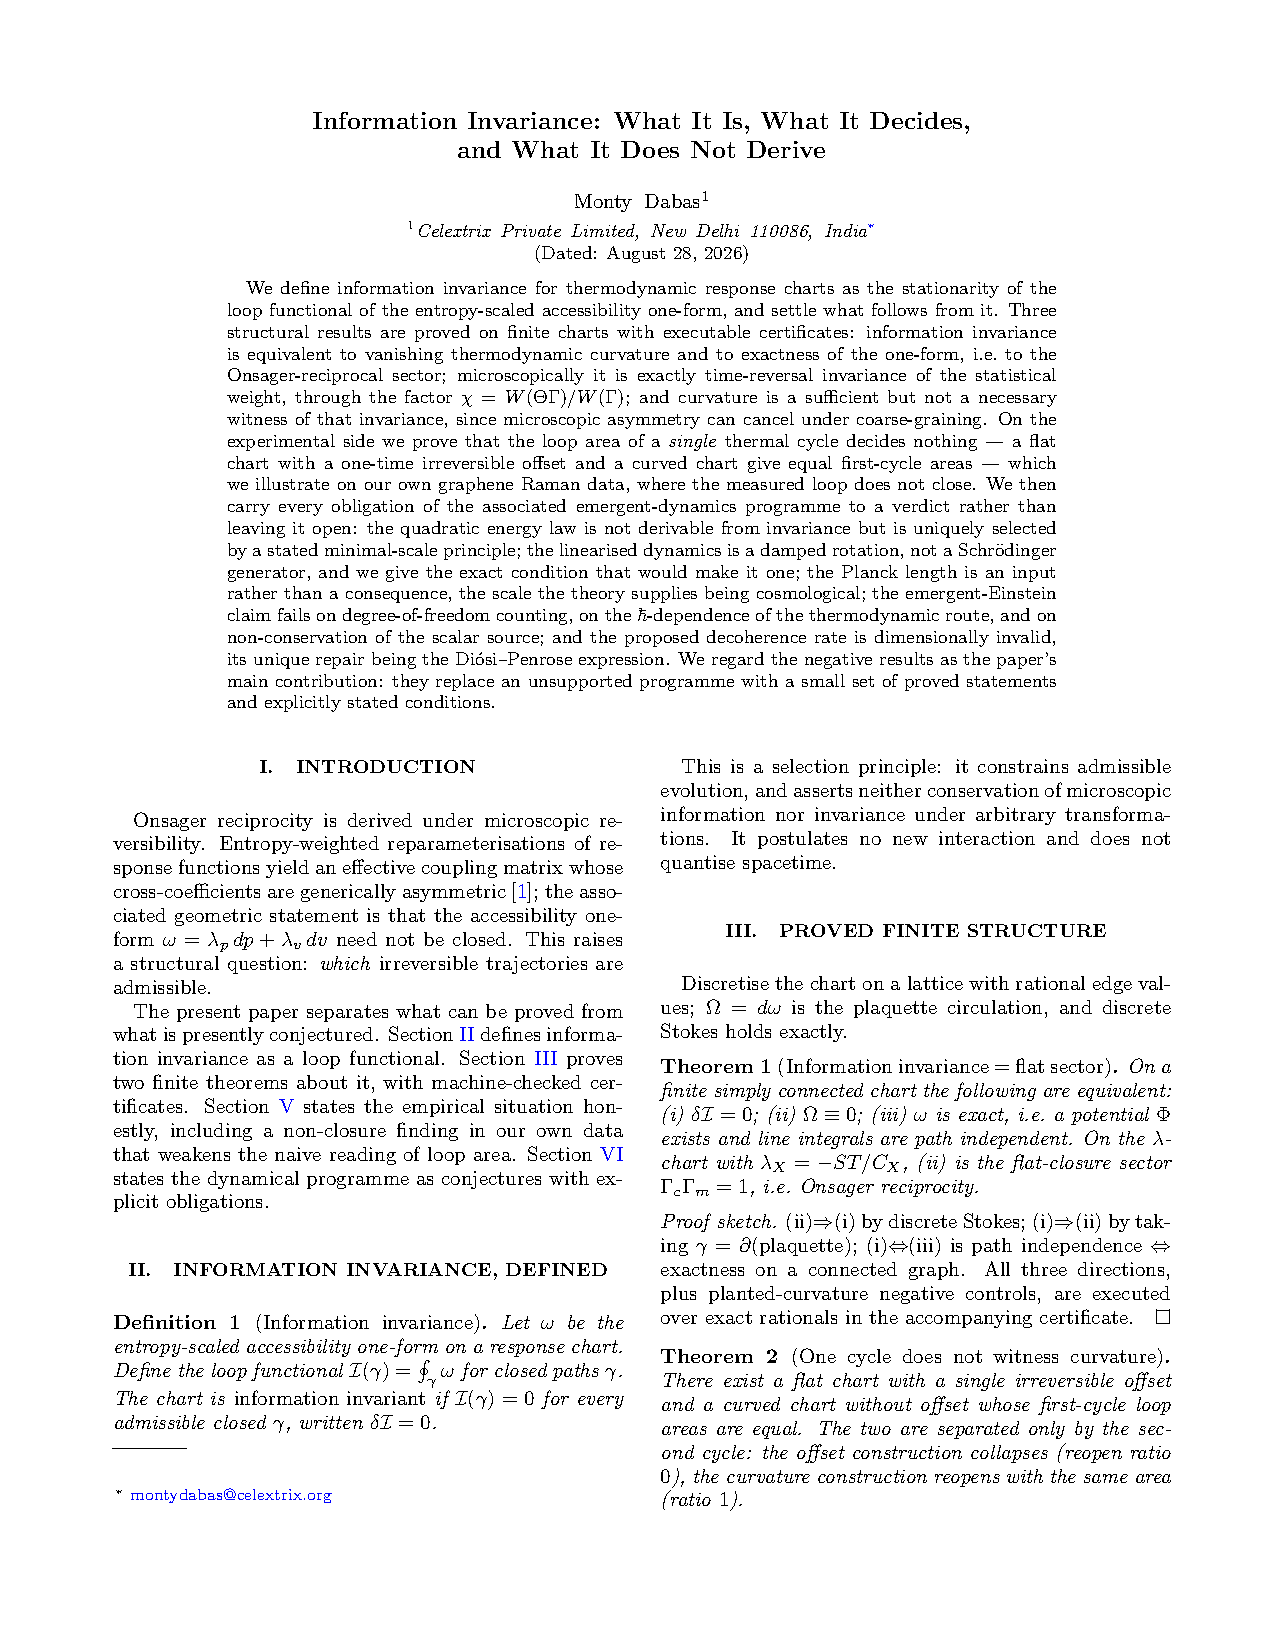
\includepdf[pages=-]{fragments/p110.pdf}

% source: Publications/papers/lambda-seam-calibration/README.md
\hypertarget{lambda-seam-calibration-lam-1}{%
\chapter{Lambda-Seam Calibration (LAM-1)}\label{lambda-seam-calibration-lam-1}}

Calibration and audit of the \textbf{legacy Λ-analytic layer} --- the
Λ-Eisenstein / Λ-mock functional-equation machinery that grew out of the
T-V-S-P compass diagram of \emph{Geometric Completion of Thermodynamic
Response} (arXiv:2603.20773) --- against exact, executable arithmetic.

The legacy program carried the compass response block

\begin{verbatim}
L = [[λp, Lpv], [Lvp, λv]],   φ = arg(Lpv / Lvp)
\end{verbatim}

(the Onsager non-reciprocity bias phase) into automorphic machinery,
producing ``Λ-functional equations'' of the form
\texttt{Ξ\_φ(s)\ =\ e\^{}\{iφ\}\ Ξ\_φ(1−s)}. That layer is exactly where the legacy
framework went silent on RH and Yang--Mills. This capsule certifies the
finite content of that layer and names the mechanism of the silence.

\hypertarget{certified-blocks-lam-1}{%
\section{Certified blocks (LAM-1)}\label{certified-blocks-lam-1}}

\begin{longtable}[]{@{}
  >{\raggedright\arraybackslash}p{(\columnwidth - 4\tabcolsep) * \real{0.3333}}
  >{\raggedright\arraybackslash}p{(\columnwidth - 4\tabcolsep) * \real{0.3333}}
  >{\raggedright\arraybackslash}p{(\columnwidth - 4\tabcolsep) * \real{0.3333}}@{}}
\toprule\noalign{}
\begin{minipage}[b]{\linewidth}\raggedright
Block
\end{minipage} & \begin{minipage}[b]{\linewidth}\raggedright
Statement
\end{minipage} & \begin{minipage}[b]{\linewidth}\raggedright
Verdict
\end{minipage} \\
\midrule\noalign{}
\endhead
\bottomrule\noalign{}
\endlastfoot
T1 & Ramanujan two-route: exact cyclotomic reduction of \texttt{c\_c(n)} in \texttt{Z{[}x{]}/Φ\_c(x)} equals \texttt{Σ\_\{d\textbar{}gcd(c,n)\}\ d·μ(c/d)} on a 1476-pair grid --- the layer the Λ-twist multiplies but never enters & PASS \\
T2 & Memory-lattice multiplicativity: \texttt{χ\_φ(n)=e\^{}\{iφΩ(n)\}} is exact integer bookkeeping --- Ω additive on all \texttt{mn\ ≤\ 400}; formal Euler product reproduces every \texttt{n\ ≤\ 300} with marker exactly \texttt{Ω(n)}, multiplicity exactly 1 & PASS \\
T3 & Theta seam certified: \texttt{θ(1/t)=√t·θ(t)} at \texttt{t=2} with two-sided directed rational enclosures, widths \texttt{\textless{}\ 1e-20} (actual agreement 30+ digits), \textbf{no floats in any verdict path} & PASS \\
T4 & Declared-phase audit: under the exact S-reindexing bijection \texttt{(c,d)→(d,−c)} on the primitive region \texttt{\textbar{}c\textbar{},\textbar{}d\textbar{}\ ≤\ 60} (8812 pairs), the coset-weight layer has \textbf{zero net change} (16512 = 16512) & PASS \\
\end{longtable}

Controls: coprimality tamper separates (T1); non-additive fake winding
detected (T2); \texttt{√3} tamper separates the enclosures with certified gap
\texttt{\textgreater{}\ 0.319} (T3); asymmetric region separates (T4).

\hypertarget{finding-lam1-f1}{%
\section{Finding LAM1-F1}\label{finding-lam1-f1}}

The \texttt{e\^{}\{iφ\}} functional-equation factor of the legacy Λ-construction is
a \textbf{declared} right S-multiplier, not a derived quantity. The legacy
canvas itself records that no homomorphism \texttt{SL(2,Z)\ →\ S¹} can realize
arbitrary φ (finite abelianization), and T4 certifies that the
coset-weight bookkeeping contributes zero net phase across the S-move.
The legacy analytic layer therefore decorated the classical substrate
with an \emph{input} phase --- which is the precise mechanism of its silence on
RH/YM: \textbf{the phase was never load-bearing}. Any native functional
equation (obligation N2) must \emph{derive} its seam-crossing phase; the
theta seam of T3 is the classical shape of that single crossing.

\hypertarget{claim-boundary}{%
\section{Claim boundary}\label{claim-boundary}}

\begin{itemize}
\tightlist
\item
  Legacy Λ-FE: declared multiplier over the classical substrate.
\item
  N1 (native continuation), N2 (native functional equation),
  N3 (identification): \textbf{OPEN}.
\item
  K₀ / L₀ / RH: \textbf{OPEN}. YM continuum gates: \textbf{OPEN}.
\item
  No claims about zeros of any L-function.
\item
  Classical anchors (Poisson summation, Jacobi theta inversion,
  SL(2,Z) coset structure, Ramanujan-sum closed form) are pinned named
  dependencies, cited and never rederived natively.
\end{itemize}

\hypertarget{certified-blocks-lam-2-derived-seam-phase}{%
\section{Certified blocks (LAM-2: derived seam phase)}\label{certified-blocks-lam-2-derived-seam-phase}}

The counterpoint to LAM1-F1 --- for a \emph{genuine} twist the seam phase is
\textbf{derived}, as finite arithmetic on the cut's residue classes:

\begin{longtable}[]{@{}
  >{\raggedright\arraybackslash}p{(\columnwidth - 4\tabcolsep) * \real{0.3333}}
  >{\raggedright\arraybackslash}p{(\columnwidth - 4\tabcolsep) * \real{0.3333}}
  >{\raggedright\arraybackslash}p{(\columnwidth - 4\tabcolsep) * \real{0.3333}}@{}}
\toprule\noalign{}
\begin{minipage}[b]{\linewidth}\raggedright
Block
\end{minipage} & \begin{minipage}[b]{\linewidth}\raggedright
Statement
\end{minipage} & \begin{minipage}[b]{\linewidth}\raggedright
Verdict
\end{minipage} \\
\midrule\noalign{}
\endhead
\bottomrule\noalign{}
\endlastfoot
T1 & Gauss magnitude exact: \texttt{\textbar{}τ(χ)\textbar{}²\ =\ q} in \texttt{ℤ{[}ζ\_L{]}} for all 34 primitive characters, moduli \{3,4,5,7,9,11,13\} (cyclic convolution + reduction mod \texttt{Φ\_L}; no floats, no complex numbers) & PASS \\
T1b & Quarter-turn instance: \texttt{τ(χ₄)²\ =\ −4} exactly --- the derived seam phase at q=4 satisfies the cut relation \texttt{ι²\ =\ −1} & PASS \\
T2 & The derivation step exact: separated-Gauss identity \texttt{Σ\_a\ χ̄(a)ζ\_q\^{}\{an\}\ =\ χ(n)τ(χ̄)} at \textbf{every} residue n for every primitive χ (335 identities), including \texttt{gcd(n,q)\textgreater{}1} where both sides vanish --- the vanishing \emph{is} primitivity & PASS \\
T3 & Derived phase certified analytically: twisted theta seam \texttt{θ\_χ(1/2)\ =\ √8·θ\_χ(2)} at q=4 with derived multiplier \texttt{τ/(i√q)\ =\ 1}, enclosures agreeing to 30+ digits & PASS \\
T4 & No conductor for the legacy twist: for every modulus \texttt{q\ ≤\ 60}, explicit congruent pair with different \texttt{Ω} --- the winding twist is a Dirichlet character of \textbf{no} modulus & PASS \\
\end{longtable}

Controls: imprimitive character mod 9 gives \texttt{\textbar{}τ\textbar{}²\ =\ 0} and fails the
derivation step at residue n=3 (both exact); multiplier tamper
(\texttt{√2} for \texttt{√8}) separates the certified enclosures with gap \texttt{\textgreater{}\ 0.58}.

\hypertarget{findings-lam2-f1f2f3}{%
\section{Findings LAM2-F1/F2/F3}\label{findings-lam2-f1f2f3}}

\textbf{F1 (template):} for primitive-character twists the FE seam phase is
finite cut arithmetic --- exact magnitude, exact derivation step, and a
certified analytic seam confirming the derived multiplier. A derived
phase is \emph{load-bearing}: tampering it separates certified enclosures.

\textbf{F2 (native hook, remark-level):} \texttt{τ(χ₄)²\ =\ −4} --- the derived phase at
q=4 is exactly the quarter turn: \texttt{(τ/√q)²\ =\ −1}, the cut's defining
relation, obtained from seam arithmetic rather than declared.

\textbf{F3 (impossibility half):} the legacy winding twist
\texttt{χ\_φ(n)\ =\ e\^{}\{iφΩ(n)\}} has \textbf{no conductor} (witness for every q ≤ 60),
so the Gauss-seam derivation route does not exist for it: the declared
phase of LAM1-F1 was \emph{forced} by the twist's own arithmetic. Together,
LAM1-F1 + LAM2-F1 state the N2 design constraint: a native functional
equation must ride a twist whose phase is derivable as finite seam
arithmetic.

\hypertarget{certified-blocks-lam-3-the-crossing-derived}{%
\section{Certified blocks (LAM-3: the crossing, derived)}\label{certified-blocks-lam-3-the-crossing-derived}}

The derivation of the \texttt{s\ ↔\ 1−s} crossing itself, executed and certified
at machine level --- theta seam → split-flip identity → manifestly
symmetric completed kernel = Euler-product side --- at points where the
native \texttt{ζ\_Σ} exists. The FE phase for ζ is the derived \texttt{+1} of the
untwisted seam: an \emph{output} of the crossing, never an input.

\begin{longtable}[]{@{}
  >{\raggedright\arraybackslash}p{(\columnwidth - 4\tabcolsep) * \real{0.3333}}
  >{\raggedright\arraybackslash}p{(\columnwidth - 4\tabcolsep) * \real{0.3333}}
  >{\raggedright\arraybackslash}p{(\columnwidth - 4\tabcolsep) * \real{0.3333}}@{}}
\toprule\noalign{}
\begin{minipage}[b]{\linewidth}\raggedright
Block
\end{minipage} & \begin{minipage}[b]{\linewidth}\raggedright
Statement
\end{minipage} & \begin{minipage}[b]{\linewidth}\raggedright
Verdict
\end{minipage} \\
\midrule\noalign{}
\endhead
\bottomrule\noalign{}
\endlastfoot
T1 & Memory-grammar values: \texttt{γ}, \texttt{ln\ 2}, \texttt{ln\ π}, \texttt{ζ(3)}, \texttt{ζ(5)} as exact-rational enclosures (recognized body + Bernoulli correction window + declared bracketed tail), widths \texttt{\textless{}\ 1e-24}, two truncation depths overlap & PASS \\
T2 & Split-flip identity at s=3: \texttt{∫₀¹\ t\^{}\{1/2\}ω\ dt\ =\ 1/6\ +\ ∫₁\^{}∞\ t\^{}\{-2\}ω\ dt}, two independent routes (incomplete-gamma series vs \texttt{E₁} route with exact rational cancellation) agreeing to 28+ digits --- the crossing step, certified & PASS \\
T3 & Completed identity at s=3: \texttt{ζ(3)/(2π)\ =\ 1/6\ +\ ∫₁\^{}∞\ (t\^{}\{1/2\}+t\^{}\{-2\})ω\ dt} & PASS \\
T4 & Second point s=5: \texttt{3ζ(5)/(4π²)\ =\ 1/20\ +\ ∫₁\^{}∞\ (t\^{}\{3/2\}+t\^{}\{-3\})ω\ dt} --- kills point-luck & PASS \\
\end{longtable}

Controls: polar-drop separates (gap \textgreater{} 1/10); seam-weight tamper
\texttt{ω(1/t)\ →\ t·ω(t)+(t−1)/2} separates (gap \textgreater{} 2/5); reflected-kernel
exponent tamper separates (gap \textgreater{} 1/200); body-only ζ separates
(memory grammar load-bearing); Bernoulli-window tamper separates.

\textbf{Note on the E₁ route:} at \texttt{c\ =\ 16π} the convergent-series route
suffers \textasciitilde22 digits of cancellation --- fatal in floats, \emph{exact} in
rationals. The capsule's positivity and width assertions at that point
are the machine witness that the arithmetic discipline is load-bearing.

\hypertarget{findings-lam3-f1f2}{%
\section{Findings LAM3-F1/F2}\label{findings-lam3-f1f2}}

\textbf{F1:} the crossing is derived end-to-end and machine-certified on the
\texttt{Re\ s\ \textgreater{}\ 1} side. Contrast chain complete across the paper:
LAM-1 --- declared phase, never load-bearing; LAM-2 --- derived phase,
load-bearing finite seam arithmetic; LAM-3 --- the derivation itself
executed, with every tamper separating certified enclosures.

\textbf{F2:} the memory grammar is load-bearing: body-only ζ(3) separates by
more than \texttt{1e-5} at widths below \texttt{1e-24} --- the public echo of ``without
memory terms there is no critical strip.''

\hypertarget{honest-boundary-lam-3}{%
\section{Honest boundary (LAM-3)}\label{honest-boundary-lam-3}}

Continuation into the critical strip via the symmetric kernel is
\textbf{definitional} here, not a native theorem. The exact remaining native
obligation for N2 is now pinned: \emph{reproduce the split-flip step (T2)
inside the cut grammar, where the theta seam is a native theorem rather
than a pinned classical anchor.} T3 is T2 composed with exact termwise
Mellin evaluation (recorded per TAUT-1); the tails on both sides share
the Euler--Maclaurin utility.

\hypertarget{reproduce}{%
\section{Reproduce}\label{reproduce}}

\begin{verbatim}
python papers/lambda-seam-calibration/certificates/lam1_seam_interface.py
python papers/lambda-seam-calibration/certificates/lam2_derived_phase.py
python papers/lambda-seam-calibration/certificates/lam3_crossing_derivation.py
python -m pytest papers/lambda-seam-calibration/tests -v
\end{verbatim}

The generator is deterministic; CI regenerates the certificate and
fails on any pin drift (\texttt{EXPECTED\_LAM1.sha256}, \texttt{EXPECTED\_LAM2.sha256}, \texttt{EXPECTED\_LAM3.sha256}).

\hypertarget{arithmetic-discipline}{%
\section{Arithmetic discipline}\label{arithmetic-discipline}}

Integers, exact rationals, exact integer polynomial arithmetic, and
directed rational intervals with relative outward rounding to 300-bit
significands. No floating point in any verdict path.

\begin{flushright}\small\texttt{Publications/papers/lambda-seam-calibration/README.md}\end{flushright}

% source: Publications/papers/lambda-seam-calibration/LINEAGE.md
\hypertarget{lineage-and-ruling}{%
\chapter{Lineage and Ruling}\label{lineage-and-ruling}}

\hypertarget{origin-chain}{%
\section{Origin chain}\label{origin-chain}}

\begin{enumerate}
\def\labelenumi{\arabic{enumi}.}
\tightlist
\item
  \textbf{T-V-S-P compass} --- the central diagram of \emph{Geometric Completion of
  Thermodynamic Response} (arXiv:2603.20773): four response channels on
  a two-dimensional equilibrium chart, response block
  \texttt{L\ =\ {[}{[}λp,\ Lpv{]},{[}Lvp,\ λv{]}{]}} with Onsager non-reciprocity
  \texttt{φ\ =\ arg(Lpv/Lvp)}.
\item
  \textbf{λ-geometry / Λ-geometric canvases} (legacy, 2024--25 era):
  projective seam spectrum \texttt{Λ±(Γ,ρ)}, stability wedge, exceptional
  (Jordan) lines, seam holonomy, and the interface conjecture
  \texttt{Φ\_hol\ =\ φ\_Λ} --- the seam holonomy as functional-equation phase.
\item
  \textbf{Λ-analytic rigor canvases} (legacy): Λ-twisted Poincaré/heat
  kernel → Mellin → unfolding/Poisson → \texttt{Ξ\_φ(s)\ =\ e\^{}\{iφ\}Ξ\_φ(1−s)},
  with Γ/π constant audits (including the half-weight Λ-mock case).
  This is the layer where the legacy framework went silent on RH and
  Yang--Mills.
\end{enumerate}

\hypertarget{ruling-mine-dont-merge}{%
\section{Ruling: MINE-DON'T-MERGE}\label{ruling-mine-dont-merge}}

Zero claims are imported from the legacy canvases. What is mined:

\begin{itemize}
\tightlist
\item
  The \textbf{shape} of Lemma 13.7 (``the Poisson step only sees the right
  S-multiplier''): the entire functional-equation content of the cut
  crossing concentrates in one move at S. LAM-1 certifies the finite
  bookkeeping half of this (T4) and the classical crossing itself (T3).
\item
  The compass-phase identification (\texttt{φ} of the response block = \texttt{φ} of
  the FE multiplier), recorded as lineage, not as a theorem.
\end{itemize}

What is explicitly \textbf{not} imported:

\begin{itemize}
\tightlist
\item
  The legacy ``Λ-functional equation'' as a result --- LAM1-F1 certifies its
  phase is declared, not derived.
\item
  All informal holonomy/transport statements of the legacy geometric
  canvases (e.g.~the informal seam-holonomy theorem and the seam
  quantization conjecture). Their finite/structural content is
  superseded by certified capsule results elsewhere in this repository
  and the framework repos (seam-integer counts, transported
  multiplicity-one crossing lines); legacy formulas in this area have
  previously failed audit and must not be cited.
\item
  All ``TTC'' sectoral specializations.
\end{itemize}

\hypertarget{relation-to-the-open-program}{%
\section{Relation to the open program}\label{relation-to-the-open-program}}

The one obligation this calibration sharpens: a native functional
equation (N2) must \emph{derive} its seam-crossing phase from the cut
grammar (memory channel included), rather than declare it. The theta
identity certified in T3 is the classical shape of that single seam
crossing; the memory-lattice bookkeeping of T2 is the exact object any
native twist rides on. Both are finite, exact, and now pinned.

\hypertarget{lam-2-addendum}{%
\section{LAM-2 addendum}\label{lam-2-addendum}}

LAM-2 supplies the constructive counterpoint: the derived-phase template
(Gauss-sum seam arithmetic, exact in cyclotomic rings) and the
impossibility half (the legacy winding twist has no conductor, so the
derivation route never existed for it). Classical anchors --- Gauss sums,
the separated-Gauss identity, the odd twisted theta functional
equation --- are pinned named dependencies; finite instances are verified
exactly, nothing is claimed as new mathematics. The native obligation
N2 remains open: what LAM-2 fixes is its design constraint.

\hypertarget{lam-3-addendum}{%
\section{LAM-3 addendum}\label{lam-3-addendum}}

LAM-3 closes the paper's contrast arc by executing the classical
derivation of the s \textless-\textgreater{} 1-s crossing with certified arithmetic on the
memory-grammar carrier, at points where the native zeta exists. The
legacy canvases attempted to build functional equations by decorating
this substrate with a declared phase; LAM-3 shows the substrate's own
phase (+1) being derived, tamper-separable at every step. The single
remaining native obligation for N2 is stated in the certificate:
reproduce the split-flip step inside the cut grammar with the theta
seam as a native theorem. Euler-Maclaurin enveloping remainders and
the theta/Mellin substrate are pinned classical anchors throughout.

\begin{flushright}\small\texttt{Publications/papers/lambda-seam-calibration/LINEAGE.md}\end{flushright}

% source: Publications/papers/poincare-calibration/README.md
\hypertarget{poincaruxe9-calibration-pc-1}{%
\chapter{Poincaré Calibration --- PC-1}\label{poincaruxe9-calibration-pc-1}}

\textbf{This is a calibration, not a proof.} The Poincaré conjecture is a proved
theorem (Hamilton--Perelman, 2003). Nothing here claims any part of it and
nothing here is new mathematics. The capsule instantiates the dictionary of
\texttt{MP\ adapters/poincare/adapter.tex} v0.2 (``Poincaré Calibration Adapter''),
whose stated purpose is to test whether the framework can carry native
hypotheses, singularity control, surgery, extinction and topological
reconstruction \textbf{without hiding any step inside a decorative closure
predicate}. PC-1 answers that for one piece --- exactly.

\hypertarget{carrier}{%
\section{Carrier}\label{carrier}}

Left-invariant metrics on \textbf{SU(2)} (deliberately the same group as the
Yang--Mills line), diagonal in a Milnor frame \texttt{g\ =\ diag(A,B,C)}. Ricci flow
is an exact rational ODE: \texttt{A\textquotesingle{}\ =\ 2{[}(B−C)²\ −\ A²{]}/(BC)} and cyclically.

\hypertarget{certified}{%
\section{Certified}\label{certified}}

\begin{longtable}[]{@{}
  >{\raggedright\arraybackslash}p{(\columnwidth - 2\tabcolsep) * \real{0.5000}}
  >{\raggedright\arraybackslash}p{(\columnwidth - 2\tabcolsep) * \real{0.5000}}@{}}
\toprule\noalign{}
\begin{minipage}[b]{\linewidth}\raggedright
\end{minipage} & \begin{minipage}[b]{\linewidth}\raggedright
Statement
\end{minipage} \\
\midrule\noalign{}
\endhead
\bottomrule\noalign{}
\endlastfoot
\textbf{T1} & \texttt{λ(g)\ =\ min\ spec(−4Δ\ +\ R)\ =\ R(g)} on any homogeneous metric; \texttt{R\ =\ {[}2(AB+BC+CA)\ −\ (A²+B²+C²){]}/(ABC)} verified \\
\textbf{T2} & \textbf{\texttt{dR/dt\ −\ 2‖Ric‖²\ ≡\ 0}} in \texttt{ℚ(A,B,C)} --- Perelman's λ-monotonicity as a \emph{polynomial identity}, with an explicit 3-term sum-of-squares witness. No analysis, no tolerance, no approximation \\
\textbf{T3} & Round solution exact: \texttt{a(t)\ =\ a₀\ −\ 2t}, \texttt{λ\ =\ 3/a}, extinction \texttt{t*\ =\ a₀/2} exactly \\
\textbf{T4} & Berger rounding exact: \texttt{du/dt\ =\ −4(x−z)/(xz)} for \texttt{u\ =\ x/z}, so \texttt{sign(du/dt)\ =\ −sign(u−1)} --- monotone convergence to round \\
\textbf{T5} & Seam readout: λ is a bottom-of-spectrum threshold object, strictly increasing ⇒ threshold crossings are irreversible (one-directional seam flow; same primitive as the YM seam-integer dock, opposite regime) \\
\end{longtable}

Controls: R-formula tamper and flow tamper both break the identity;
round-case specialization consistent; \texttt{‖Ric‖²\ \textgreater{}\ 0} strictly; collapse
boundary sampled and recorded as an obstruction-tower entry, not claimed.

\hypertarget{honest-remainder}{%
\section{Honest remainder}\label{honest-remainder}}

Untouched, restated from the adapter's obstruction tower: surgery and
neck/cap data; non-collapsing, κ-solutions, canonical neighbourhoods;
singularity classification off the homogeneous carrier; finite-time
extinction in general; topological reconstruction; \textbf{and the Poincaré
conjecture itself --- NOT CLAIMED}. Hamilton--Perelman stays a pinned named
dependency, cited never rederived (CIRC-1).

The homogeneous carrier is precisely where surgery and collapse are
absent. That is why this is a calibration.

\hypertarget{reproduce}{%
\section{Reproduce}\label{reproduce}}

\begin{verbatim}
python papers/poincare-calibration/certificates/pc1_lambda_monotonicity.py
python -m pytest papers/poincare-calibration/tests -v
\end{verbatim}

\begin{flushright}\small\texttt{Publications/papers/poincare-calibration/README.md}\end{flushright}

% source: Publications/papers/recognition-seam-topology/README.md
\hypertarget{rst-1-recognition-seam-topology-the-exact-spine-certified}{%
\chapter{RST-1 --- Recognition-Seam Topology: the exact spine, certified}\label{rst-1-recognition-seam-topology-the-exact-spine-certified}}

Source: \textbf{``Recognition-Seam Topology and Daggered Index Geometry''}
(M. Dabas, July 2026, arXiv source v1), sections 2--7. The paper is the
mature front door of the RH programme (MP PR \#94 lineage) and carries its
own claim ledger; this capsule certifies the ledger's \emph{proved} finite,
circle-operator and model statements in exact rational arithmetic --- no
floats, no transcendental evaluation, no truncation posing as a limit ---
and records the analytic layer as declared-not-certified.

\hypertarget{blocks}{%
\section{Blocks}\label{blocks}}

\begin{longtable}[]{@{}
  >{\raggedright\arraybackslash}p{(\columnwidth - 4\tabcolsep) * \real{0.3333}}
  >{\raggedright\arraybackslash}p{(\columnwidth - 4\tabcolsep) * \real{0.3333}}
  >{\raggedright\arraybackslash}p{(\columnwidth - 4\tabcolsep) * \real{0.3333}}@{}}
\toprule\noalign{}
\begin{minipage}[b]{\linewidth}\raggedright
Block
\end{minipage} & \begin{minipage}[b]{\linewidth}\raggedright
Content
\end{minipage} & \begin{minipage}[b]{\linewidth}\raggedright
Key exact fact
\end{minipage} \\
\midrule\noalign{}
\endhead
\bottomrule\noalign{}
\endlastfoot
T1 & Cut-stable topology, Eye quotient, seam, curvature defect (§2) & All 64 subsets checked; τ = \{∅, \{0..3\}, \{4,5\}, X\} is a genuine non-discrete topology; seam = zero-cost locus with an off-seam point of \emph{infinite} cost; the defect fires exactly where an unlawful declared composite breaks recognized path equality \\
T2 & Rotation instead of gluing (§3.2, §4) & Orientation target factors through \textbf{no} map on the glued quotient; one bit of sheet label repairs it; recognition equality ≠ state identity; reflected side target is target-null exactly on the fixed locus \\
T3 & Rotation-induced involution (§3.3) & J\_U self-adjoint involution with orthogonal projections for the rational 3-4-5 rotation; \textbf{bridge:} J\_\{U=I\} is the cut swap --- fourth certified presentation of the derived involution (EMK-1 T1, EMK-G1 T1, EMK-T1 T1) \\
T4 & Flow generator (§3.4, §5) & Cayley loop as an exact polynomial matrix in h: \textbf{L\_h = I + h²{[}D₁,D₂{]} exactly} (the nilpotent loop terminates at degree 2 --- stronger than the paper's O(h³)); commuting control gives L\_h ≡ I; eigenmode law certified term-by-term with no exponential evaluated; covariance defect ⟺ conjugation invariance \\
T5 & Derived dagger algebra (§6) & R₀* = −R₀ but R₀♯ = +R₀ over Gaussian rationals: dagger self-adjointness is \textbf{not} Hilbert self-adjointness; leakage three-way equivalence on all 256 grid matrices \\
T6 & Circle carrier (§7) & \textbf{sf = Wind = ind = q} for q ∈ \{−3,−1,0,1,2,5\}: rational crossing times with a proof the window is exhaustive for the \emph{full} Fourier spectrum; winding by exact signed crossings on the Pythagorean parametrization; Toeplitz kernel/cokernel read off the shift \\
T7 & Staircase negative control (§5.8) & Length exactly 2 for every n while sup-distance² ≤ 1/(2n²): limit of lengths ≠ length of limit; not evidence of curvature \\
\end{longtable}

\hypertarget{findings}{%
\section{Findings}\label{findings}}

\begin{itemize}
\tightlist
\item
  \textbf{F1 (derived involution, fourth presentation).} The rotation-induced
  J\_U at U = I \emph{is} the cut swap. Geometry involution (EMK-G1), algebra
  seam reflection (EMK-1), tensor cut-swap (EMK-T1) and now the
  sheet-exchange of rotation transport are one derived object. The
  involution is never primitive --- the paper's derived-involution
  principle is now a certificate, not a remark.
\item
  \textbf{F2 (curvature = non-closure, without limits).} The commutator-loop
  residue is a polynomial-coefficient identity, and for nilpotent
  generators the loop \emph{equals} I + h²{[}D₁,D₂{]} with no higher terms.
\item
  \textbf{F3 (index without truncation).} The circle identity
  sf = Wind = ind = q is certified with every count exact and exhaustive.
\item
  \textbf{F4 (memory is one bit, minimally).} Gluing destroys orientation
  targets; the minimal repair is a single binary sheet label.
\end{itemize}

\hypertarget{claim-boundary}{%
\section{Claim boundary}\label{claim-boundary}}

Analytic theorems of the source (damped trace-class family Thm 8.8,
undamped strip classification Thm 9.1, Schatten thresholds, archimedean
defect) are \textbf{declared, not certified} --- they are analytic, outside
exact rational verification, and are not consumed. No arithmetic meaning
is assigned to q. The represented seam is \textbf{not} identified with the
critical line. Model zeros are \textbf{not} zeros of ξi. \textbf{Riemann
hypothesis: ABSTAIN} --- exactly as the source paper states.

\hypertarget{next}{%
\section{Next}\label{next}}

RST-2 will certify the finite arithmetic/transfer/fusion spine
(§8--14): Möbius pressure extraction, radical recognition current,
prime-shell transfer and asymmetric leakage, zero-identification
boundary, and the Surya/Weil sign fusion on rational-eigenvalue models.

\hypertarget{reproduce}{%
\section{Reproduce}\label{reproduce}}

\begin{verbatim}
python certificates/rst1_recognition_seam_topology.py
python -m pytest tests -v
\end{verbatim}

The certificate regenerates byte-identically; its sha256 is pinned in
\texttt{certificates/EXPECTED\_RST1.sha256}.

\begin{center}\rule{0.5\linewidth}{0.5pt}\end{center}

\hypertarget{rst-2-arithmetic-and-fusion-spine-814-certified}{%
\chapter{RST-2 --- Arithmetic and fusion spine (§8--14), certified}\label{rst-2-arithmetic-and-fusion-spine-814-certified}}

Same folder, second capsule, 35 further tests (70 total in this folder).

\begin{longtable}[]{@{}
  >{\raggedright\arraybackslash}p{(\columnwidth - 4\tabcolsep) * \real{0.3333}}
  >{\raggedright\arraybackslash}p{(\columnwidth - 4\tabcolsep) * \real{0.3333}}
  >{\raggedright\arraybackslash}p{(\columnwidth - 4\tabcolsep) * \real{0.3333}}@{}}
\toprule\noalign{}
\begin{minipage}[b]{\linewidth}\raggedright
Block
\end{minipage} & \begin{minipage}[b]{\linewidth}\raggedright
Content
\end{minipage} & \begin{minipage}[b]{\linewidth}\raggedright
Key exact fact
\end{minipage} \\
\midrule\noalign{}
\endhead
\bottomrule\noalign{}
\endlastfoot
T1 & Sampled reflection, spectral blindness (§8.2--8.3) & ρ(s)=1−s swaps the rational sample pairs exactly; seam projection provably independent of the anti-seam component \\
T2 & Weights, leakage norm, crossings (§8.4, §8.7) & Equal pair weights ⟺ swap isometric (both directions); finite leakage norm² = max aₖ² attained; avoided family has det = −((η−c)²+µ²) ≤ −µ² \textless{} 0 --- zero never in spectrum \\
T3 & Arithmetic recognition (§10) & \textbf{The formal-log move:} log n carried as the vector of prime exponents, so (L1)∗µ = Λ is an exact integer-vector identity for all n ≤ 60 --- no logarithm evaluated. Λ-current 0 on every anti-seam class; contamination → exactly ϵe₆ \\
T4 & Prime-shell transfer (§11) & U A = A P, JA = A, P₋A = 0, JU*J = U exactly; asymmetric leakage = ((w\_R−w\_L)/2)(e\_R−e\_L) per shell; \textbf{converse-fails witness:} a common seam-sector error is invisible to the anti-seam current \\
T5 & Zero-identification boundary (§13) & Paired determinant: zeros ±λⱼ \textbf{with multiplicity by exact division} (double level → double zero); log-derivative identity in cross-multiplied polynomial form; nonvanishing factor preserves the divisor; working Z1/Z2/Z3 obstruction validator \\
T6 & Surya/Weil fusion (§14) & Feshbach congruence M = Sᵀdiag(A,F)S as an exact identity with negative witnesses transported through it; \textbf{Surya without square roots} (squared amplitude x²/(1+x²) on x\textless0): A\_SS = 0 ⟺ W₀ ⪰ 0; seam charge additive, = −spectral flow, every crossing downward; µ = 1 strictly outside the charge; principal holonomy blindness (m mod 1 = 0 ∀m) \\
\end{longtable}

\textbf{Findings.} F5: the projection-blindness thread now spans four capsules
(UGD-1 T4, EMK-T1 T5, RST-2 T1, principal holonomy) --- the visible
coordinate never carries the full state. F6: the anti-seam current
detects only the \emph{antisymmetric} discrepancy --- the seam sector needs its
own audit (converse-fails witness). F7: the Surya sign problem is
decidable entirely in squared-amplitude arithmetic --- no functional
calculus square root is ever needed for the vanishing question.

\textbf{Claim boundary.} Gaussian damping form and 1/√2 normalization are
declared; W₃, Weil↔RH, the completed parity/Feshbach reduction and the
even compact operator are imported by the source and NOT certified here;
fusion gates F1--F5 remain OPEN; Zmodel→Zξ forbidden. \textbf{RH: ABSTAIN.}

\begin{verbatim}
python certificates/rst2_arithmetic_fusion_spine.py
python -m pytest tests -v
\end{verbatim}

\begin{center}\rule{0.5\linewidth}{0.5pt}\end{center}

\hypertarget{emk-top-1-the-vault-topology-appendix-exact-spine}{%
\chapter{EMK-TOP-1 --- The vault topology appendix, exact spine}\label{emk-top-1-the-vault-topology-appendix-exact-spine}}

Source: \texttt{APPENDIX\_EMK\_TOPOLOGY\_RIGOROUS.tex} in the private vault, with
the sheet-rotation subsection of the Euler information--curvature
appendix. \textbf{This is a different object from RST-1} (see LINEAGE.md):
the paper gives cut-stable topology and index calibration; the appendix
builds seam \emph{cohomology}. 29 tests; 99 in this folder.

\begin{longtable}[]{@{}
  >{\raggedright\arraybackslash}p{(\columnwidth - 4\tabcolsep) * \real{0.3333}}
  >{\raggedright\arraybackslash}p{(\columnwidth - 4\tabcolsep) * \real{0.3333}}
  >{\raggedright\arraybackslash}p{(\columnwidth - 4\tabcolsep) * \real{0.3333}}@{}}
\toprule\noalign{}
\begin{minipage}[b]{\linewidth}\raggedright
Block
\end{minipage} & \begin{minipage}[b]{\linewidth}\raggedright
Certifies
\end{minipage} & \begin{minipage}[b]{\linewidth}\raggedright
Result
\end{minipage} \\
\midrule\noalign{}
\endhead
\bottomrule\noalign{}
\endlastfoot
\textbf{T1} & The I, R, K system is closed and finite (order \textbf{8}, \{±1\}×\{I,R,K,RK\}); explicit KIR words that are the \textbf{identity under the shadow projection while their holonomy is −I} --- visibly closed loops that do not recognition-close; the lawful ledger closes them exactly & PASS \\
\textbf{T2} & On an explicit complex (square + diagonal, one face filled) d₁d₀ = 0 and \textbf{H¹ rank exactly 1}; a closed cochain has \textbf{equal} charge on homologous cycles and zero on boundaries; a non-closed one is provably not a class function & PASS \\
\textbf{T3} & The additive log-determinant cochain certified \textbf{multiplicatively} --- no logarithm evaluated. The corollary as an exact witness: a loop whose \textbf{global determinant returns exactly} while subcycle charges are 6 and 1/6 & PASS \\
\textbf{T4} & The \textbf{trichotomy} exact / closed-non-exact / open, decided by exact rank, with a witness of each and an explicit β for the exact one. \textbf{Bridge:} CFE-U's H¹ = 0 means the middle class is \emph{empty} on the response complex --- the trichotomy is about the complex, not a universal law & PASS \\
\textbf{T5} & Sheet-rotation class with an exact cocycle, phase carried as an \textbf{exponent in ℤ/K} (never a root of unity): a loop with total turn 0 mod K --- visible phase return --- but sheet index 2 and winding 6 & PASS \\
\textbf{T6} & Seam survival ⟺ every \textbf{active} sector closes; shadow-only survival witness, exact and wrong ledgers separated, and monotonicity in the active set (so it must be declared before the verdict) & PASS \\
\end{longtable}

Protocol --- the space tuple, seam module, tolerances, eight-component
residue vector, commit policy --- and the declared information-curvature
tensor I\^{}GE remain \textbf{declared, not certified}.

\begin{flushright}\small\texttt{Publications/papers/recognition-seam-topology/README.md}\end{flushright}

% source: Publications/papers/recognition-seam-topology/LINEAGE.md
\hypertarget{lineage-rst-1}{%
\chapter{Lineage --- RST-1}\label{lineage-rst-1}}

\begin{itemize}
\tightlist
\item
  \textbf{Primary source:} ``Recognition-Seam Topology and Daggered Index
  Geometry --- Foundations for an EMK Route to the Riemann Hypothesis''
  (M. Dabas, July 2026), arXiv source v1 PDF. Sections certified: 2--7.
\item
  \textbf{Paper lineage (as recorded in its Appendix B):} MP RH branch stack
  PRs \#50, \#62--\#82, \#89--\#91, \#94 (front door); EMK-UGD Vault
  sheet-rotation development (commits c7255dfa\ldots, 24bb86a2\ldots, a22053a8\ldots,
  40f23dbe\ldots, cbcecdbf\ldots); imported native X3 fusion lineage (PRs \#127,
  \#200, \#202, \#205, \#208--\#212) --- the X3 layer is \emph{not} consumed by
  RST-1 (deferred to RST-2's finite spine).
\item
  \textbf{Vault cross-reference:} APPENDIX\_EMK\_TOPOLOGY\_RIGOROUS
  (EMK-UGD-Provisional-Vault, recognition\_seam\_calculus\_master tree)
  overlaps sections 2--6; a file-level diff is pending repo access and
  will be recorded here when done. The paper is treated as source of
  truth (it is the mature front door and postdates the appendix).
\item
  \textbf{Certified companions in this corpus:} EMK-1, EMK-2, UGD-1, EMK-T1
  (papers/emk-ugd-algebra); EMK-G1 (papers/emk-recognition-geometry).
  The derived-involution thread now spans all of them plus RST-1 T3.
\item
  \textbf{Prior executable version:} NONE found for the paper's exact spine.
  This is the first certification.
\end{itemize}

\begin{flushright}\small\texttt{Publications/papers/recognition-seam-topology/LINEAGE.md}\end{flushright}

% source: Publications/papers/representation-complete-native-seam-integer/README.md
\hypertarget{representation-complete-native-seam-integer-paper}{%
\chapter{Representation-Complete Native Seam Integer Paper}\label{representation-complete-native-seam-integer-paper}}

\hypertarget{source-of-record}{%
\section{Source of record}\label{source-of-record}}

Repository: \texttt{Parveen117/MP}\\
Branch: \texttt{agent/paper-source-floor-five-by-five-theorem}\\
Draft PR: \texttt{\#244}

\hypertarget{expected-release-contents}{%
\section{Expected release contents}\label{expected-release-contents}}

\begin{verbatim}
source/       complete LaTeX submission tree
pdf/          final compiled PDF
metadata/     arXiv metadata and claim ledger
\end{verbatim}

\hypertarget{current-claim-boundary}{%
\section{Current claim boundary}\label{current-claim-boundary}}

\begin{verbatim}
SOURCE FLOOR S_(.01,-) >= .008 I               PROVED
SOURCE INVERSE NORM <= 125                      PROVED
HERMITIAN RANK-AT-MOST-FIVE REDUCTION           PROVED
FINAL OUTWARD ACCEPTANCE THEOREM                PROVED
ACTUAL OUTWARD FIVE-BY-FIVE VALUE               OPEN
CONTROLLED eta_j -> 0                           OPEN
RIEMANN HYPOTHESIS                              ABSTAIN
\end{verbatim}

Do not publish a Zenodo-linked release until the updated PDF has been compiled and placed in \texttt{pdf/}.

\begin{flushright}\small\texttt{Publications/papers/representation-complete-native-seam-integer/README.md}\end{flushright}

% source: Publications/papers/yang-mills-certified-benchmark/README.md
\hypertarget{yangmills-certified-benchmark-ym-1}{%
\chapter{Yang--Mills Certified Benchmark (YM-1)}\label{yangmills-certified-benchmark-ym-1}}

First rung of resuming the MP Yang--Mills adapter with the certified RNKE
machinery: the reduced finite-cutoff gap of the SU(2) one-holonomy Wilson
benchmark, previously a float, is now an exact two-sided rational enclosure.

\hypertarget{certified-statement}{%
\section{Certified statement}\label{certified-statement}}

For the normalized SU(2) Wilson convolution operator on class functions
(source: \texttt{MP/adapters/yang\_mills/cutoff\_gap\_benchmark.tex}), with exact
character spectrum \texttt{lambda\_j(beta)\ =\ I\_\{2j+1\}(beta)/I\_1(beta)}:

\begin{verbatim}
Delta_red(a=1, beta=2) = -log( I_2(2) / I_1(2) )
  in [0.83672330623158891305006780105454768321... ]  (width < 1e-30, exact ℚ)
\end{verbatim}

Verdict engine: directed rational interval arithmetic only. No floats in any
verdict. Controls: (C1) \texttt{lambda\_1} strictly inside (0,1) hence gap strictly
positive; (C2) tampering \texttt{I\_2\ -\textgreater{}\ I\_3} produces a separated bracket; (C3)
width budget.

\hypertarget{claim-boundary-fail-closed}{%
\section{Claim boundary (fail-closed)}\label{claim-boundary-fail-closed}}

\begin{itemize}
\tightlist
\item
  CERTIFIED: the reduced finite-cutoff benchmark number only.
\item
  NOT CERTIFIED / OPEN: full-lattice gap, theta-graph interacting transfer,
  ultraviolet/infinite-volume uniformity, OS continuum reconstruction, the
  Clay existence and mass-gap predicate. Adapter verdict remains \texttt{hold}.
\end{itemize}

\hypertarget{ledger}{%
\section{Ledger}\label{ledger}}

\begin{longtable}[]{@{}
  >{\raggedright\arraybackslash}p{(\columnwidth - 2\tabcolsep) * \real{0.5000}}
  >{\raggedright\arraybackslash}p{(\columnwidth - 2\tabcolsep) * \real{0.5000}}@{}}
\toprule\noalign{}
\begin{minipage}[b]{\linewidth}\raggedright
Item
\end{minipage} & \begin{minipage}[b]{\linewidth}\raggedright
Status
\end{minipage} \\
\midrule\noalign{}
\endhead
\bottomrule\noalign{}
\endlastfoot
YM-1 reduced gap enclosure (a=1, beta=2) & PASS (pinned) \\
YM-2 interacting theta-graph gap, certified small coupling (kappa \textless{} Delta\_red/6) & PASS (pinned) \\
YM-3 first-order crossing direction: rank-one, A\textless-\textgreater B transported, slope lambda\_half/4 & PASS (pinned) \\
YM-4 symmetry-protection theorem {[}S,T\_kappa{]}=0 + finite-kappa certified lower bounds & PASS (pinned) \\
YM-5 certified TWO-SIDED gap at finite kappa, beyond the sandwich threshold (Kill-Lemma realization) & PASS (pinned) \\
YM-6 seam-integer dock: EXACT eigenvalue counts on the native 5x5, certified to kappa=1/2 (D03 congruence) & PASS (pinned) \\
YM-7 V7 carrier: kappa=7/10 unlocked (exact count), certified 7-eigenvalue crossing curves & PASS (pinned) \\
YM-8 CAPSTONE: theta-graph gap is a THEOREM at every coupling (certified kernel floors + pinned Jentzsch anchor); remaining Millennium content = uniformity in the cutoff & PASS (pinned) \\
YM-9 FIRST UNIFORMITY: exact heat-kernel refinement family; free gap exactly cutoff-independent; interacting uniform bound 3/8 along a declared trajectory & PASS (pinned) \\
YM-10 blindness ledger (SPECTRAL-1/2 framework): exact multiplicity law, exact probe counts, composition ledger, YM-9 T4 correction & PASS (pinned) \\
YM-11 three gate verdicts on the toy carrier: gauge CLOSED; volume/IR SPLIT (free closed, sandwich route proven insufficient, critical volume exact); universality SPLIT (counting closed, metric open) & PASS (pinned) \\
YM-12 the T03 move: positivity SQUARE-SOURCED (classical anchor demoted to simplicity-only); volume+cutoff-uniform interacting gap 3/8 on the factorized chain; governance capsule & PASS (pinned) \\
YM-13 verification-overlap beta audit: beta 4/5 -\textgreater{} 3/5 via independent witnesses (CF Bessel, compound-interest exp, det/trace inertia); three lineage overlaps retained with refusal notes; RH remains lowest at 1/5 & PASS (pinned) \\
YM-14 interaction-overlap dock, first carrier: bridged pair --- overlap seam rank-one and swap-transported (same theta integral), certified k=1 to kappa=1/2, overlap price kappa*lam/4 on one line; kappa=1 carrier limit recorded & PASS (pinned) \\
YM-15 1D block-transfer dock opened: exact closed form of the chain compression for EVERY m (vacuum f0\^{}\{m-1\}, A-line f0\^{}\{m-1\}·KMS\_m(r), r=I2/I1; SU(2) convolution lemma, machine-checked as a formal polynomial identity m=2..8, no truncation remainder); m-UNIFORM ratio bracket λ(1−r)/(1+r)\textless ρ\_m\textless λ(1+r)/(1−r), certified positive normalised gap for all m at κ≤1; κ=2 fails closed. A-line carrier ONLY --- complement not bounded & PASS (pinned) \\
YM-16 chain dock: exact B-factorisation ⇒ gap(S\_m) ≤ Δ\_red for ALL m,κ (m-uniform upper bound, exact eigenvector); vacuum volume bracket f0\^{}\{m−1\} ≤ λ₁ ≤ e\^{}\{κ(m−1)\}; certified two-sided gap (ratio ≤ 9/10) of S\_m for m ≤ m\emph{(κ) --- m}=13 (κ=1/8), 7 (1/4), 4 (1/2) --- with m* computed exactly and matched by the dock; m*+1 refused. Sup route provably non-uniform: death volume has coordinates & PASS (pinned) \\
YM-17 interleaving seam: m\_κ = B\_odd·B\_even; each dressed half-chain is a tensor product of the two-site chain at 2κ ⇒ product spectrum ⇒ gap ratio EXACTLY m-uniform (pair ratio certified ≤ 9/10 at κ≤1/2; bracket {[}1,3{]} honest at κ=1); vacuum bracket narrowed to rate κ² (per-bridge upper end 0.125→0.030 at κ=1/8); whole volume problem reduced to ONE inequality: λ₁(T) vs σ₁(X)σ₁(Y) (vacuum tracking of interleaved halves) & PASS (pinned) \\
YM-18 CALIBRATION + DESIGN: enlarged exact carrier W'\_m (vacuum + sites + bridge-pairs, dim 2m) gives certified Rayleigh lower bounds on λ₁(T\_A,m), m=2..6; per-bridge vacuum rate φ\_m\^{}lo is m-independent to \textasciitilde1e-5 (0.002177 @κ=1/8, 0.008698 @1/4, 0.03461 @1/2) --- vacuum tracking behaves as a clean per-bridge rate; bracket width = looseness of the upper end. Cluster dock DESIGNED (monomers = odd pairs at 2κ, activities = even bridges, KP on a line) --- no claim & PASS (calibration, pinned) \\
YM-19 Dobrushin dock --- \textbf{DEMOTED to ANCHORED} (governance rule: no classical borrowing; T3 rests on a cited Dobrushin/Föllmer anchor, same fate as YM-8 Jentzsch). T1 (coefficient bound) and T2 (α\textless1 arithmetic) are native and stand; the m-uniform GAP claim is WITHDRAWN until derived natively. Was: on the bounded-overlap chain --- Dobrushin coefficient C\_ij ≤ 1−1/δ² (elementary, proved), δ\_s = e\^{}\{2κ\} exact, δ\_t ≤ (1+S\_a)/(1−S\_a) certified; α = 2(1−1/δ\_t²)+2(1−1/δ\_s²) \textless{} 1 ⇒ (pinned anchor: Dobrushin/Föllmer/Künsch covariance decay; extraction lemma proved) λ₂/λ₁ ≤ α for EVERY m. Certified gap/step ≥ 0.263 (a=6,κ=1/16), ≥ 0.145 (a=8,κ=1/8, ON YM-9's trajectory θ=1/64), ≥ 0.235 (a=12,κ=1/8); refused at (6,1/8),(4,1/16),(10,1/4). Coupling ceiling of the route exact: κ \textless{} log2/4. STANDING CORRECTION to YM-17 T3 (vacuum tracking insufficient; correlation-decay route replaces it). NOT uniform in the cutoff (δ\_t→∞ as a→0) & ANCHORED (pinned, not a native theorem) \\
YM-20 NATIVE ORIGIN AUDIT: machine-checked origin ledger for YM-1..19 in the framework's vocabulary (carrier = COORDINATE\_SHADOW throughout; counting = NATIVE\_DERIVED throughout; anchors: YM-8 and YM-19 demoted imports, YM-17 SV-Weyl as technique). CAYLEY FORM certified: YM-15 ceiling (1+r)/(1−r) and YM-19 δ\_t are Exp\_Σ(A\_Σ(y)) (F00-G Thm 5.1 pinned) with seam coordinates r, S\_a; native odd-series log agrees with YM-1 route to 1e-20; uniform gap in native form = −Log\_Σ(λ) − A\_Σ(r). Bessel coefficients = native factorial series (F00-E Lemma 2.1 shape); Haar identification = the shadow. NAMED YM-21: bridge-local recognition-energy contraction under the seam-involution flow (F00-E Thm 6.2) & PASS (pinned) \\
\textbf{YM-F1 THE CHAIN AS A RECOGNITION FABRIC (native carrier)}: T1 SU(2) = unit sphere of the EMK block over C\_Σ --- span\{I, R, ιK, ιRK\} is Hamilton's quaternion algebra, det = Δ∥+Δ⊥ becomes the quaternion norm (twisted seam channels), χ½ = 2×identity-sector coefficient; T2 chain = ladder fabric, bridge faces = plaquette holonomies H\_l = A\_i⁻¹A\_\{i+1\}; T3 Recognition-Stokes EXACT on the chain (interior rungs cancel, E\_int = 0, orientation tamper bites); T4 action = sum of face residues ρ\_l = 1−Tr H\_l/2 ∈ {[}0,2{]}, weight = Exp\_Σ(κ(m−1))·Exp\_Σ(−κΣρ). Source: vault fabric appendix + EMK-1 + F00-E. Remaining shadow: Haar ↔ Φ\_Σ (declared). Native form of YM-21 posed on the fabric & PASS (pinned) \\
YM-21 THE TILING LAW (native, on the fabric): STANDING CORRECTION to YM-F1's posed question (boundary residue cannot control face residue --- witness g, g⁻¹, certified); the right object is the tiling. T2 Stokes sub-telescoping ⇒ YM-15 entry = r\^{}\{\#faces crossed\}: SPATIAL decay along the chain exactly geometric, rate −Log r, every m. T3 leading-order TIME two-point = (λ·KMS\_m(r))\^{}t, bracketed λ\textsuperscript{t((1∓r)/(1±r))}t for every m ⇒ YM-15/20's uniform rate −Log λ − A\_Σ(r) DERIVED as a tiling count (t=1..6, m=2..8 inside bracket). T4 remainder named natively: higher-content/branching tilings, expansion parameter = face-coefficient ladder r\_j (certified decreasing: r\_½ ≫ r\_1 ≫ r\_\{3/2\}); uniform convergence = native cluster statement & PASS (pinned) \\
\textbf{YM-22 THE TILING RATE SURVIVES THE CUTOFF}: on the heat-kernel family along κ=θa, the time-face log is EXACTLY 3a/4 (no transcendental), so the leading tiling rate per unit time γ(a) = 3/4 − A\_Σ(r(θa))/a. Certified over SIX DECADES a=1\ldots1e-6 at θ=1/16: \textbf{23/32 ≤ γ(a) ≤ 3/4 for every a} --- the limit 3/4 − θ/2 is a uniform LOWER bound in the cutoff (approached from above); KMS bracket holds with λ\_a for m=2..8 at every a ⇒ leading-order rate uniform in volume AND cutoff simultaneously. Beats YM-9's sandwich 3/4 − 6θ by factor 12 in the θ-coefficient; trajectory ceiling θ \textless{} 3/2 (θ=2 refused). Higher face coefficients per unit time r\_1/a, r\_\{3/2\}/a → 0: in the cutoff limit only j=½ branching survives. SCOPE: leading tiling order & PASS (pinned) \\
\textbf{YM-23 THE WEAK-COUPLING TURN}: T1 tiling route has an EXACT weak-coupling boundary --- ladder collapses (r\_½,r\_1,r\_\{3/2\} = 0.970, 0.922, 0.859 at κ=50: no small parameter), leading rate sign change at r\_c(a) = tanh(3a/8) in native Cayley form, κ\_c(a) bracketed (1.574 @a=1, 0.759 @1/2, 0.376 @1/4, 0.188 @1/8), and on a DECLARED AF-shaped trajectory κ = ¼log(1/a) the route is left at a = 1/8 --- the continuum lies outside the tiling route. T2 native linearization: ρ = 2s/(1+s) in the stereographic chart; odd(H₁H₂) = p₁+p₂+½{[}p₁,p₂{]} EXACTLY --- the commutator is the only non-additive term = EMK-1 T5 / RST-1 T4 curvature on the fabric. T3 EXACT NEGATIVE: the abelianized fabric's softest spatial stiffness ≤ 12κ/(m(m+1)) (Rayleigh identity certified m=2..40) --- gapless in volume. T4 native statement: a weak-coupling gap lives entirely in the commutator sector (non-healable curvature) --- the mass gap is non-perturbative, said in the framework's words & PASS (pinned) \\
YM-24 ABELIAN SUBFABRIC + NON-ABELIAN RESIDUE (exact algebra, no gap claim): T1 commuting faces = F00-E's circular Euler orbit, compose by the native addition law, Stokes additive in the Euler coordinate (the rotor chain), m=2..8 on rational circle points; T2 non-abelian residue = Gram defect & p×q \\
YM-25 THE DIRECTION-CHANGE SECTOR: two exact negatives --- the time kernel is direction-blind (bi-invariant: one scalar per spin-j block, d\_j² coefficients, refinement-invariant) and the strong-coupling carriers are direction-blind (class functions, rotation-invariant: structural SPECTRAL-1 blindness) --- and one exact positive: direction change between adjacent faces IS the 6j recoupling (MP gold/01 seed), squared overlaps between (12)3 and 1(23) schemes exactly {[}{[}1/4,3/4{]},{[}3/4,1/4{]}{]}, unitary, no √ evaluated (RST-2 discipline), singlet tamper breaks unitarity. REDUCTION: a weak-coupling gap can live only in the intertwiner transfer & PASS (pinned) \\
\textbf{YM-26 DOCK TO theorum/28 (Recognition-Complete Finite-to-Infinite Cut Theorem)} --- owner's correction: the framework's own convergence machinery. Dictionary: P\_n = A-line carrier (YM-15), Q\_n = complement, floor λ₁ ≥ f₀\^{}\{m−1\}, threshold μ = νf₀\^{}\{m−1\}, e\_n = ‖QSQ‖/μ, N₊(B\_n−I) = Haynsworth inertia; outward certificate e\_n \textless{} 1 ∧ inertia count = 1 ⇒ λ₂ \textless{} νλ₁. T1: LAWFUL (e\_n present, not a shadow certificate) for every m ≤ m\emph{(κ) = 13, 7, 4 at κ = 1/8, 1/4, 1/2. T2: e\_n(m) certified increasing, crosses 1 exactly at m}+1 --- theorum/28's hypothesis 3 (memory-channel Cauchy bound uniform in m) is NOT YET BUILT; full hypothesis ledger 1--7 written in the theorem's vocabulary. T3: via the tiling law, item 3 reduces to a Cauchy bound uniform in m for the multi-insertion content-½ memory channel (the j=½ branching sector) & PASS (pinned) \\
\textbf{YM-27 DOCK TO RH-FRAMEWORK T01} (owner: use the RH journey's proved results, cite them): T1 the sup route IS T01-E4C (bounded native simple multiplier, U\_Σ(w) = e\^{}κ exactly; YM-16's e\_n reproduced to the last digit) ⇒ theorum/28 hypothesis 3 = a memory-channel bound beating T01-E4C by a factor uniform in m --- measured slack per face 56.5 / 27.8 / 13.5 at κ = 1/8, 1/4, 1/2 (YM-18 calibration vs E4C price). T2 the abelian subfabric is a T01-E5A rational UGD packet: wrap law = rotor-chain composition, winding = seam memory μ; (g,g⁻¹) witness vs full-turn fabric have the same visible boundary but μ = 0 vs 1 --- the native form of EMK-1 winding. T3 the Haar shadow of YM-F1 is exactly RH's OPEN T01-E5C/E6 --- YM inherits RH's item, invents none; aliasing structure of class functions on E1 grids certified (exact for n \textgreater{} 2j). T4 T01-B/C recognition energy = chain vacuum form, floor f₀\^{}\{m−1\} & PASS (pinned) \\
\textbf{YM-28 T01-E4D ON THE CHAIN} (RH-Framework PR \#19 applied): T1 the mean law is EXACT with zero deviation on single insertions --- I\_rec(W·χ½(A\_i)) = f₀(2κ)\^{}\{m−1\} for every m (formal identity, χ₁ branch dies at the open end); T2 two insertions: deviation = r₁(2κ)\^{}\{ & i−j \\
YM-29 CLOSED-FORM VACUUM FLOOR FOR EVERY m: native face-independence lemma (bridge faces independent contents, W a product over faces ⇒ face-product integrals factorise; fusion-rule certified: ∫wχ½ = 2f\_½, ∫wχ½² = f₀+3f₁); T0\^{}\{1/2\}χ½(H\_ℓ) = λχ½(H\_ℓ); ansatz ψ = 1 + cΣχ½(H\_ℓ) gives λ₁ ≥ f₀\^{}\{m−1\}·Q\_m(c\emph{) in closed form for ALL m, Q\_m \textgreater{} 1 always, \textasciitilde4λ²r²(m−1) for m ≫ 1/(4λ²r²) (Q₂₀₀₀ = 2.58 / 6.99 / 24.1). Honest: linear floor moves the dock's m} by 0 --- the floor at the TRUE rate (0.000228/face margin, YM-28) needs the product ansatz, whose T-expectation is the one-time-step ladder = 6j recoupling contraction & PASS (pinned) \\
\textbf{YM-30 THE 2-ROW RECOUPLING ENGINE --- BUILT AND VALIDATED}: exact surd arithmetic (Q adjoined √), Clebsch--Gordan by Racah's closed form (no floats), 3j, three-matrix-coefficient vertex integral, ε-removal of conjugates, ladder (one-time-step fabric) evaluated as a transfer over cut indices with label sums folded in. V1 every evaluation rational (surds cancel --- the built-in consistency check); V2 one plaquette = 1/d\_a²; V3 single-row limit recovers the YM-15 chain; V4 two plaquettes: Σ\_c d\_c N = 1/4 and the split d₀N₀ : d₁N₁ = 1/4 : 3/4 = YM-25's recoupling squares, now from the engine; V5 rail-swap and reversal symmetry. FIRST USE (calibration, κ=1/8, content ≤ 1, point coefficients): the W\^{}\{1/2\}-dressed vacuum for T'\,' = W\textsuperscript{\{1/2\}T0W}\{1/2\} beats the old floor f₀\^{}\{m−1\} by a GEOMETRIC factor 1.000732 per face (m=2..6) --- floor rate 0.002685/face \textgreater{} YM-18's bound 0.002177 \textgreater{} E4D excitation rate 0.001949: margin 0.000736/face; single-face excitation (c ≠ 0) does not help & PASS (pinned) \\
\textbf{YM-31 OUTWARD m-UNIFORM DRESSED VACUUM FLOOR --- theorum/28 ITEM 6 AT THE TRUE RATE}: trial φ = W\^{}\{1/2\}·(W\_pt/W) with W\_pt a product of rational truncated faces (no error by definition); numerator = ladder ⟨W\_pt, T0 W\_pt⟩ (YM-30 engine), rung truncation is a rigorous LOWER bound (T0 = Π\_i Σ\_c λ\_c Π\_c: a sum of nonnegative projection terms, monotone in λ\_c); denominator ∫W\_pt²/W = {[}Σ d\_jd\_kd\_l f\_j\^{}pt f\_k\^{}pt (−1)\^{}\{2l\} f\_l N\_jkl{]}\^{}\{m−1\} exact with outward l-tail; NATIVE LOG-CONVEXITY Z\_m² ≤ Z\_\{m−1\}Z\_\{m+1\} (Z\_m = ⟨g, S\^{}\{m−2\}g⟩, S = C\^{}\{1/2\}M\_K C\^{}\{1/2\} symmetric PSD, cut-square inequality) ⇒ ratio nondecreasing ⇒ \textbf{λ₁(S\_m) ≥ FLOOR\_\{m₀\}·(ρ\_lo/I\_hi)\^{}\{m−m₀\} for every m ≥ 6}, rung tail at m₀ bounded (5.9e-9). Per-face floor rate \textbf{0.002685 / 0.010722 / 0.042607} at κ = 1/8, 1/4, 1/2 vs old floor 0.001952 / 0.007802 / 0.031089 and E4D excitation rate 0.001949 / 0.007742 / 0.030161 --- margin \textbf{0.000736 / 0.002980 / 0.012446 per face}, uniformly in m & PASS (pinned) \\
YM-32 DRESSED SINGLE-INSERTION ENERGY, m-UNIFORM (engine extended to rung insertions via CG reduction of 4-valent vertices; validated: j=0 reproduces YM-30, one-rail insertion vanishes, reversal identity, mixed-rung tamper smaller): E\_m(p) = ⟨W\_ptχ½(A\_p), T0 W\_ptχ½(A\_p)⟩/⟨W\_pt,T0W\_pt⟩ exact for m=2..7, all p --- bulk value m-independent to \textless{} 1e-6, ends differ; E\_bulk = 0.43368 / 0.43532 / 0.44171 at κ = 1/8, 1/4, 1/2, i.e.~λ·(1 + 1.27e-3 / 5.05e-3 / 1.98e-2), inside YM-15's bracket (I first wrote `below λ'; the engine corrected me). Dressed denominator factorises (rung insertion free) ⇒ the J=½ sector's dressed excitation/vacuum ratio is exactly E\_bulk, uniformly in m --- a certified LOWER bound on that sector's top, not an upper bound on λ₂ & PASS (pinned) \\
YM-33 t-ROW FABRIC ENGINE + EXACT TIME TWO-POINT FUNCTION (owner's framing: time carries no infinity, only the flow λ\^{}τ = Exp\_Σ(−τ·gap); expand the space coupling only): general cut transfer over t rails with rungs contracted up the column (interior vertices 5-leg: two rungs, two faces, insertion --- two CG fusions); validated: t=2 reproduces YM-32 exactly, t=1 the chain, 3-row fabrics rational with exact time reflection. Dressed sequence a\_τ = ⟨φ, T'\,'\_pt\^{}τ φ⟩ and vacuum z\_τ exact for τ=1,2, m=5..8: ratio sequence ρ₁ = E\_bulk (YM-32), ρ₂ ≥ ρ₁, and the SECOND-ORDER connected correction δ₂ = ρ₂ − ρ₁ is a BULK CONSTANT --- 0.00076998 / 0.00305278 / 0.01178845 at κ = 1/8, 1/4, 1/2 --- with boundary influence decaying geometrically: moving an end from distance 2→3 shifts δ₂ by 1.3e-9 (either end, identically), 3→4 by 1.6e-12, ratio certified in {[}r²/2, 2r²{]}. The framework's own strong-coupling series for the gap, order by order as exact rationals, m-uniform with exponentially localised edges. Lower-bound side (Rayleigh data) --- item 3's upper bound still open & PASS (pinned) \\
YM-34 E4D-C RESTATED (native Laplace principle): the iterated multiplier WITHOUT smoothing, q\_n = ∫wⁿ/∫wⁿ⁻¹, is strictly increasing to sup w = e\^{}\{2κ\} (certified n ≤ 60) --- so E4D-C as written in the RH ledger (deviation control of the multiplier iterated on one state) is unprovable, and the exponential of YM-16/26 is this growth. WITH the time kernel between multiplications the ratio is nondecreasing (log-convexity) and converges to λ₁(K\textsuperscript{\{1/2\}WK}\{1/2\}) = f₀(1+δ), δ = 0.003582 / 0.014032 / 0.051911 (κ=1/8,1/4,1/2) vs sup price 0.274 / 0.598 / 1.405. E4D-C is restated for the alternating product (K\textsuperscript{\{1/2\}M\_wK}\{1/2\})ⁿ: λ₂/λ₁ ≤ 1−δ\_gap uniform in m --- the vacuum side of this is YM-31; only the excitation side is open & PASS (pinned) \\
Remaining: theorum/28 item 3 --- the memory channel's OPERATOR norm (not basis-state norms) uniform in m, via the same engine (E4D-C quadratic form on content-½); with YM-31's floor the dock's e\_n becomes (‖QTQ‖/FLOOR) and the sup numerator is the last exponential; (interval coefficients, content tail, Perron bound on the column transfer → m-uniform floor at rate ≥ 0.00268) and the E4D-C quadratic form on content-½ via the same engine; (exact rational ladder evaluations) --- closes item 6 at the true rate AND item 3 (E4D-C quadratic form on content-½) in one build; E4D-C on SUPERPOSITIONS of content-½ basis states (a quadratic-form statement on the multi-insertion channel) = theorum/28 item 3 (content-½ multi-insertion memory channel, Cauchy-uniform in m); (weak) YM-27 the intertwiner (spin-network) transfer on the chain fabric --- recoupling matrices as weak-coupling tiling weights, floor uniform in m? (declared: chain \textasciitilde{} O(4)-type rotor model in 1+1D, continuum gap at the frontier for every method); (strong) FULL-ORDER tiling convergence uniform in m and a (j=½ branching); (weak) the COMMUTATOR-RESIDUE TRANSFER on the fabric --- does the non-abelian sector alone carry a gap; AF trajectory derivation; (convergence of the face-coefficient tiling expansion) --- the cluster statement in fabric language; then (replace the borrowed decay anchor by program machinery --- square-sourcing/seam count/flow generator; generalized Euler flow and EMK/UGD sections to be read first); then uniformity in the CUTOFF a→0 of the volume-uniform gap (Dobrushin degrades as the heat kernel sharpens) --- this is now the sharp wall; AF trajectory, tightness, OS, non-triviality, metric universality, 2D lattice, Clay & OPEN \\
(superseded as the main route) cluster dock YM-18 proper: certified Kotecký--Preiss radius for the interleaving polymer gas with two-site pairs as monomers; per-bridge/local control in the content basis --- certified strong-coupling cluster radius), 2D lattice, AF trajectory, tightness, OS reconstruction, non-triviality, metric universality, Clay predicate & OPEN \\
Continuum existence / mass gap & OPEN \\
\end{longtable}

\hypertarget{reproduce}{%
\section{Reproduce}\label{reproduce}}

New in YM-2: for beta=2 the interacting theta-graph transfer
\texttt{T\_kappa\ =\ M\^{}\{1/2\}(K\ x\ K)M\^{}\{1/2\}} has a certified positive spectral gap for
every coupling \texttt{0\ \textless{}=\ kappa\ \textless{}\ kappa\_0\ =\ Delta\_red/6\ =\ 0.13945388...}, via the
min-max sandwich \texttt{m\_-\ T\_0\ \textless{}=\ T\_kappa\ \textless{}=\ m\_+\ T\_0} with
\texttt{m\_+/m\_-\ =\ e\^{}\{6\ kappa\}} from \texttt{\textbar{}Tr\ U\textbar{}\ \textless{}=\ 2}. At \texttt{kappa\ =\ 1/8} the reduced gap
is certified \texttt{\textgreater{}=\ 0.08672330623...}. Fail-closed above threshold.

\begin{verbatim}
python papers/yang-mills-certified-benchmark/certificates/ym1_certified_gap.py
python papers/yang-mills-certified-benchmark/certificates/ym2_theta_interacting_gap.py
python -m pytest papers/yang-mills-certified-benchmark/tests -v
\end{verbatim}

New in YM-3 (exact, zero coupling): the free top-excited eigenspace is exactly
two-dimensional; the exact theta integral \texttt{Int\ chi12(A)chi12(B)chi12(AB\^{}-1)\ =\ 1/2}
splits it at first order with derivatives \texttt{+-lambda\_half/4}; the vacuum derivative
is exactly 0. Hence \texttt{r\textquotesingle{}(0)\ =\ lambda\_half/4} (certified \texttt{0.10828185668...}), the
first-order CROSSING DIRECTION is the single symmetric line
\texttt{chi12(A)+chi12(B)} --- rank-one and transported by the graph symmetry --- and
YM-2's sandwich slope is slack by the exact factor 24.

Single-command reproduction (regenerates and pins all three):

\begin{verbatim}
python papers/yang-mills-certified-benchmark/certificates/ym12_square_sourced.py
\end{verbatim}

YM-12 transplants the RH journey's decisive step (T03: re-source
positivity as a square with declared defects) to Yang-Mills:

\begin{itemize}
\tightlist
\item
  \textbf{T1} manifest square: \texttt{T\_kappa(a)\ =\ S*S} with
  \texttt{S\ =\ {[}K\_\{a/2\}\ x\ K\_\{a/2\}{]}\ m\_\{kappa/2\}} --- both factors are the program's
  own halved-parameter objects (YM-9 semigroup + YM-5 doubling).
  Positivity is now \textbf{square-sourced}; YM-8's Jentzsch anchor is demoted
  to top-eigenvalue \emph{simplicity} only. The compressed defect
  \texttt{A\ -\ N*G\^{}\{-1\}N} is exactly a Gram of \texttt{(I-P)S\ phi} --- a source-restriction
  object, the T03 shape.
\item
  \textbf{T2} on the theta chain \texttt{L\_m} (vertex-glued, no shared faces) the
  transfer tensor-factorizes exactly, so \texttt{lambda\_2/lambda\_1} is
  \texttt{m}-independent, and with YM-9: \texttt{Delta(L\_m,\ a,\ a/16)\ \textgreater{}=\ 3/8} for
  \textbf{every} \texttt{m} and \textbf{every} \texttt{a} --- an interacting gap uniform in volume
  and cutoff simultaneously. This closes YM-11 gate 2's interacting half
  on the factorized family and localizes the remaining volume obstruction
  to \textbf{interaction overlap} (shared faces): the chain (no sharing) is
  uniform, \texttt{B\_n} (complete sharing) kills the sup route, and a physical
  lattice's bounded sharing sits strictly between the two certified
  extremes.
\item
  \textbf{T3} governance capsule (RH 07-20 analog): claim/consumption chain for
  YM-1..12, standing corrections (YM-9 T4 amendment, YM-8 anchor
  demotion), and a do-not-reopen list --- machine-checked for completeness.
\end{itemize}

YM-11 takes three dependency-map gates and gives each an exact verdict on
the toy carrier --- the generalized theta (``n-banana'') graphs \texttt{B\_n}, two
vertices joined by \texttt{n} edges, so \texttt{b\_1\ =\ n-1} holonomies and
\texttt{F(n)\ =\ n(n-1)/2} plaquettes; \texttt{B\_3} is the theta graph of YM-1..10.
\textbf{These are toy-carrier verdicts, not Clay-sense closures}, and two of
the three are partly negative.

\begin{itemize}
\tightlist
\item
  \textbf{Gauge --- CLOSED.} Tree gauge-fixing on a connected graph is exact (no
  Gribov obstruction), leaving \texttt{b\_1\ =\ E-V+1} holonomies and a residual
  diagonal \texttt{G} acting by conjugation, so gauge-invariant states are
  exactly \texttt{L\^{}2(G\^{}\{b\_1\})\^{}Ad}. For \texttt{B\_3} that \textbf{is} the carrier every
  capsule has used --- now certified rather than assumed, with Wilson loops
  spanning it and YM-10's multiplicity law counting them.
\item
  \textbf{Volume / IR --- SPLIT.} The \emph{free} reduced gap is \texttt{C\_(1/2)\ =\ 3/4} for
  every \texttt{n} and every \texttt{a}: volume- \textbf{and} cutoff-uniform, closed. The
  \emph{interacting} sandwich gives \texttt{Delta\ \textgreater{}=\ C\_(1/2)\ -\ 2\ F(n)\ theta}, which
  degrades quadratically in \texttt{n}: at \texttt{theta\ =\ 1/16} the bounds are \texttt{3/8}
  (n=3), exactly \texttt{0} (n=4), \texttt{-1/2} (n=5). The route is \textbf{proven
  insufficient} for volume-uniformity, with the critical volume computed
  exactly. What a replacement must do is named: control the interaction
  per-plaquette (dock route, YM-6) rather than by a global sup (envelope
  route, YM-5) --- the same lesson one level up.
\item
  \textbf{Universality --- SPLIT.} For the whole regulator class
  \texttt{K\ =\ sum\_j\ d\_j\ c\_j\ chi\_j} with \texttt{c\_j\ \textgreater{}\ 0}, the \textbf{counting layer}
  (content grading, multiplicity law, carrier dimensions, blindness
  ledger, probe counts) depends only on SU(2) representation theory and
  is therefore regulator-independent --- closed, and it means YM-10's
  ledger is kinematics, not a choice of action. The \textbf{metric layer} (the
  gap value) genuinely differs between regulators (witnessed) and remains
  the real universality gate.
\end{itemize}

YM-10 applies the source-restriction framework of the companion
manuscripts \emph{When Spectra Forget Order} and \emph{Stable Recovery Beyond
Spectral Blindness} to our own compressions. Every dock computes on a
compressed carrier \texttt{V}; in that language \texttt{V} is a source restriction, so
the honest question is not whether the complement bound is tight but
whether the carrier is \textbf{blind} to the target.

\begin{itemize}
\tightlist
\item
  \textbf{T1} exact multiplicity law \texttt{m(j1,j2)\ =\ min(2j1,2j2)+1} on the
  Ad-invariant sector --- it reproduces \texttt{dim\ V5\ =\ 5} and \texttt{dim\ V7\ =\ 7}
  independently, and re-derives YM-6's \texttt{(1/2,1/2)} two-dimensionality from
  representation theory rather than from the Gram matrix.
\item
  \textbf{T2 correction to YM-9 T4} (self-audit): YM-9's uniform count counted
  \emph{contents}; \texttt{k\_Sigma} counts \emph{eigenvalues with multiplicity}. At \texttt{s\ =\ 2}
  that is 4 versus 5. Both are \texttt{a}-independent, so YM-9's uniformity
  conclusion is unaffected --- only the arithmetic. YM-9 is amended to
  report both.
\item
  \textbf{T3/T4} blindness ledger and exact probe count
  \texttt{rank(Pi\_s\ \textbar{}\ ker\ E)\ =\ b(V,s)}. Result worth noting: \texttt{b(V5,\ s)\ =\ 0} for
  \texttt{s\ \textless{}=\ 2} --- the YM-6 carrier is \textbf{exactly blindness-free in its own
  threshold window}, so that choice was correct, not lucky. At \texttt{s\ =\ 3},
  V5 needs 6 probes, V7 needs 4, V9 needs 0 more than V7 minus 4.
\item
  \textbf{T5} composition ledger: blindness is nonincreasing along
  \texttt{V5\ ⊂\ V7\ ⊂\ V9} with nonnegative stage increments.
\item
  \textbf{T6} the whole ledger depends only on contents and Casimir levels, so
  it is exactly \texttt{a}-independent --- one ledger covers the entire YM-9
  refinement family.
\end{itemize}

Honest remainder: the ledger is exact for the \textbf{free} target; the
interacting faces mix the content grading, so \texttt{b(V,s)} is a lower bound
there and YM-6/7's declared truncation remainder is the extra obligation.

YM-9 --- the program's first statement that is uniform in the cutoff rather
than at a fixed cutoff. Switching the link action from Wilson to the
HEAT KERNEL \texttt{K\_a(g)\ =\ sum\_j\ d\_j\ e\^{}\{-a\ C\_j\}\ chi\_j(g)} makes refinement
EXACT (\texttt{K\_a\ *\ K\_b\ =\ K\_\{a+b\}}; n links of spacing a/n compose to one link
of spacing a with no discretization error), and the cutoff dependence then
cancels identically:

\begin{itemize}
\tightlist
\item
  \textbf{T2} free reduced gap \texttt{=\ C\_(1/2)\ =\ 3/4} EXACTLY for every \texttt{a\ \textgreater{}\ 0};
\item
  \textbf{T3} along the declared trajectory \texttt{kappa(a)\ =\ theta*a},
  \texttt{Delta(a,\ kappa(a))\ \textgreater{}=\ 3/4\ -\ 6*theta} for EVERY \texttt{a\ \textgreater{}\ 0} --- at
  \texttt{theta\ =\ 1/16} a cutoff-independent gap of exactly \textbf{3/8}; fail-closed
  at \texttt{theta\ \textgreater{}=\ 1/8};
\item
  \textbf{T4} the seam count \texttt{k(a,\ e\^{}\{-as\})} is exactly \texttt{a}-independent
  (combinatorial), so the dock's threshold grammar transports across the
  whole family at once;
\item
  \textbf{T5} Wilson contrast, computed: at fixed \texttt{beta} the reduced gap grows
  like \texttt{1/a} and diverges --- no cutoff-independent gap without a running
  coupling.
\end{itemize}

Honest remainder (in-certificate): the trajectory is DECLARED not derived
(the physical one is fixed by asymptotic freedom, \texttt{beta\ \textasciitilde{}\ log(1/a)}, not
modelled); the graph is FIXED (no infinite-volume growth); the heat-kernel
action is a CHOICE (universality gate open); \texttt{Delta} is a reduced graph
gap, not a reconstructed physical mass gap. Net movement: one gate from
``untouched'' to ``touched on a toy carrier''.

Capstone (YM-8): the interacting theta-graph transfer has a strictly
positive spectral gap at EVERY coupling --- certified pointwise kernel
floors (\texttt{k\ \textgreater{}=\ e\^{}\{-3\ kappa\}\ {[}c0\^{}\{-1\}\ e\^{}\{-beta\}{]}\^{}2\ \textgreater{}\ 0}, exact enclosures)
plus the pinned classical Jentzsch/Krein-Rutman anchor (simple Perron
eigenvalue; CIRC-1 discipline: cited, never rederived). Quantified window
\texttt{kappa\ in\ {[}0,\ 7/10{]}} carries exact counts and enclosures (YM-2..7). The
honest remainder is named exactly: nothing here is uniform in the lattice;
a gap at every fixed cutoff is compatible with the gap closing in the
continuum limit --- the fixed-regulator lesson. The Millennium content is
precisely the open uniformity/OS/vacuum gates of the MP dependency map.

New in YM-7: carrier enlarged to V7 (adds \texttt{chi\_1(A),\ chi\_1(B)}; Gram stays
block-diagonal, all seven exact T0 eigenvectors), dropping the complement
top from \texttt{lambda\_1} to \texttt{lambda\_1*lambda\_half} (certified ordering) --- which
UNLOCKS the previously refused \texttt{kappa\ =\ 7/10} cell: exact seam count
\texttt{k\_Sigma\ =\ 1} at \texttt{(7/10,\ 13/10)}. Also ships certified brackets for all
seven compressed eigenvalue curves (inertia bisection; every step an exact
LDL count), published with honest kappa-drift --- adopting the RH-line's
post-pause lesson that limited-denominator ``exact constants'' are never
promoted from bisection.

New in YM-6 (framework-native): the gap becomes an exact threshold COUNT
\texttt{k\_Sigma(kappa,mu)\ =\ N(spec(T\_kappa)\ \textgreater{}\ mu)} via a Haynsworth congruence ---
the D03 ``infinite ko finite'' move --- on the native 5x5 carrier
\texttt{\{1,\ chi12(A),\ chi12(B),\ chi12(A)chi12(B),\ chi12(AB\^{}-1)\}} (all exact T0
eigenvectors; exact Gram has a single 1/2 overlap). Certified exact counts:
\texttt{k=1} at (kappa,mu) = (1/8,3/5), (1/4,3/5), (1/2,1) --- so
\texttt{lambda\_2\ \textless{}=\ mu\ \textless{}\ lambda\_1} EXACTLY, past YM-5's reach --- and constant
count across the window = no seam spectral flow (thermodynamics/02
instance). The (7/10,5/4) cell is honestly REFUSED (bracket {[}1,5{]}).

New in YM-5: certified TWO-SIDED spectral gap of the interacting theta
transfer at finite coupling --- including BEYOND YM-2's sandwich threshold
\texttt{kappa\_0\ =\ 0.1394...}. Complement control uses the exact doubling identity
\texttt{m\_kappa\^{}2\ =\ m\_\{2\ kappa\}}: \texttt{\textbar{}PMQ\textbar{}\^{}2\ \textless{}=\ lammax(P\ m\_\{2k\}\ P\ -\ (P\ m\_k\ P)\^{}2)},
with \texttt{\textbar{}QSQ\textbar{}\ \textless{}=\ lambda\_half\^{}2\ e\^{}\{3k\}} and a Weyl bound. Certified rows
(ratio upper bound, gap lower bound): kappa=1/8: 0.5003, gap\textgreater=0.6924;
kappa=1/4: 0.5610, gap\textgreater=0.5781; kappa=3/10: 0.5867, gap\textgreater=0.5332.
Fail-closed at kappa=1. Lineage: realizes the old lambda-manuscripts'
Kill-Lemma skeleton unconditionally (see LINEAGE.md); no claim imported.

New in YM-4: (T1) the graph swap S:(A,B)-\textgreater(B,A) commutes with T\_kappa for
EVERY coupling --- \texttt{Tr(BA\^{}-1)\ =\ Tr(AB\^{}-1)} on SU(2) --- so YM-3's rank-one
crossing line \texttt{chi12(A)+chi12(B)} is symmetry-protected at all kappa: a
theorem, not a first-order accident. (T2) first certified finite-kappa
spectral data from the exact character expansion
\texttt{exp{[}(k/2)TrU{]}\ =\ sum\ d\_j\ f\_j\ chi\_j}, \texttt{f\_j\ =\ 2\ I\_\{2j+1\}(k)/k}, with exact
Clebsch-Gordan ring arithmetic, the exact pairing tensor
\texttt{Int\ chi\_p(A)chi\_q(B)chi\_r(AB\^{}-1)\ =\ delta\_\{p=q=r\}/d\_p}, and a certified
truncation remainder. Sector-resolved lower bounds on the grid show the
swap-even branch rising and the swap-odd branch falling with coupling.

CI runs exactly that one command plus pin diff and pytest.

\hypertarget{ym-35-t54-energy-version-commutator-remainder-e4d-c-with-the-rkf-operator-ladder}{%
\section{YM-35 --- T54′ energy version + commutator remainder (E4D-C with the RKF operator ladder)}\label{ym-35-t54-energy-version-commutator-remainder-e4d-c-with-the-rkf-operator-ladder}}

Framework inputs: theorum/54 (constant-μ chain is exactly its uncovered case --- \texttt{sum\_mu\_diverges}), theorum/50 A4 (polarization visibility = YM-28's superposition gap), theorum/53 (energy, not mass), theorum/51 + 61 (commutator calculus). On the fabric, with the YM-30 engine as the only evaluator:

\begin{itemize}
\tightlist
\item
  \textbf{T1 locality} --- \texttt{{[}K\^{}\{1/2\},\ B\_l{]}} vanishes on states with no content at sites l, l+1; non-adjacent face pairs do not mix (site content exactly ½). Commutator support is \texttt{\{l−1,\ l+1\}} --- bridge-local, every m.
\item
  \textbf{T2 exact adjacent commutator energy} --- \texttt{E\_Σ({[}K\^{}\{1/2\},B\_l{]}\ B\_\{l+1\})\ =\ λ²·(3/4)·(1−√λ₁)²}, κ- and m-independent (site weights 1/4 : 3/4 = YM-25 recoupling squares, from the engine).
\item
  \textbf{T3 T54′ ratio theorem (commuting model, exact m ≤ 8)} --- vacuum and excitation carry the same per-face factor; ratio exactly m-independent; \texttt{Σμ\textless{}∞} not needed for a ratio.
\item
  \textbf{T4 second-order remainder} --- relative size ρ = μ²·(3/4)(1−√λ₁)² = 2.9e-4 / 1.2e-3 / 4.6e-3 at κ = 1/8, 1/4, 1/2 (a = 1); kill criterion ρ \textless{} 1/10 passed.
\end{itemize}

\textbf{Verdict:} E4D-C's excitation bound opens at the first non-commutative order --- the first obstruction is an exact local number, not a sup. \textbf{Not done:} the full face expansion (all words, contents j ≥ 1) --- the worldline cluster problem (YM-33). E4D-C OPEN. Pin \texttt{EXPECTED\_YM35.sha256}.

\hypertarget{ym-36-t54-on-the-fabric-at-content-uxbd-face-word-carrier}{%
\section{YM-36 --- T54′ on the fabric at content ½ (face-word carrier)}\label{ym-36-t54-on-the-fabric-at-content-uxbd-face-word-carrier}}

The alternating product \texttt{K\^{}\{1/2\}\ M\_w\ K\^{}\{1/2\}} compressed to ALL superpositions of content-½ face insertions (2\^{}\{m−1\} orthonormal words), exact rational matrices m = 2..6 at μ = 1/32, 1/16, 1/8 (declared rational-square kernel √λ½ = 11/16, √λ₁ = 3/8; YM-33 engine with per-column face labels). Excitation/vacuum ratio ρ\_m increases with geometrically decaying increments (consecutive-increment ratios in {[}2/5, 3/5{]} certified); under declared q ≤ 2/3 the m-uniform limit is bracketed, e.g.~ρ∞ ∈ {[}0.2225014, 0.2225544{]} at μ = 1/32. The top eigenvector is a genuine superposition (single-insertion weight 0.98 / 0.92 / 0.73), yet exceeds the one-face ratio by only 0.24 \% / 0.93 \% / 3.5 \% --- superpositions open no gap-closing channel at content ½. \textbf{Boundary:} compressed-operator statement (interlacing: lower bounds), contents j ≥ 1 outside the carrier (first effect = YM-35 commutator, \textasciitilde μ²), m ≤ 6. E4D-C OPEN; it holds at content ½ on this carrier in compression with a geometric tail. Pin \texttt{EXPECTED\_YM36.sha256}.

\hypertarget{ym-37-the-space-transfer-m-uniformity-of-the-dressed-time-two-point-ratio-as-a-theorem}{%
\section{YM-37 --- The space transfer: m-uniformity of the dressed time two-point ratio as a theorem}\label{ym-37-the-space-transfer-m-uniformity-of-the-dressed-time-two-point-ratio-as-a-theorem}}

\textbf{(a) refused with witness.} theorum/53 T4 bounds cut-square \emph{weights} (\texttt{d\_k\ ≤\ S\_kk}); a block with every diagonal ≤ μ can still have λmax \textgreater{} μ (2×2 witness, exact). So ``complement λmax from T53 weights'' is not available; item 3's upper half stays OPEN.

\textbf{What is a theorem.} Every YM-33/36 quantity is \texttt{⟨boundary,\ M\ τ\^{}\{m−1\}\ boundary⟩} for one column map τ = B⁻¹M (native quaternion carrier: faces/rungs are class functions of products, so only dot products appear; Haar = rational S³ moments; cut space = harmonic degree ≤ 2 per rail). τ commutes with simultaneous conjugation and with the centre of SU(2) acting on all rails; both boundary vectors are even, so everything lives in the even invariant sector: dim 8 (t = 2), 52 (t = 3). Validated \textbf{exactly} against \texttt{ym33.fabric\_partition}. σ₁, σ₂ of the symmetric pencil (M, B) bracketed by exact inertia (fraction-free Bareiss, Jacobi sign rule); q := σ₂/σ₁ certified:

\begin{longtable}[]{@{}
  >{\raggedright\arraybackslash}p{(\columnwidth - 12\tabcolsep) * \real{0.1429}}
  >{\raggedright\arraybackslash}p{(\columnwidth - 12\tabcolsep) * \real{0.1429}}
  >{\raggedright\arraybackslash}p{(\columnwidth - 12\tabcolsep) * \real{0.1429}}
  >{\raggedright\arraybackslash}p{(\columnwidth - 12\tabcolsep) * \real{0.1429}}
  >{\raggedright\arraybackslash}p{(\columnwidth - 12\tabcolsep) * \real{0.1429}}
  >{\raggedright\arraybackslash}p{(\columnwidth - 12\tabcolsep) * \real{0.1429}}
  >{\raggedright\arraybackslash}p{(\columnwidth - 12\tabcolsep) * \real{0.1429}}@{}}
\toprule\noalign{}
\begin{minipage}[b]{\linewidth}\raggedright
κ
\end{minipage} & \begin{minipage}[b]{\linewidth}\raggedright
q (t = 2)
\end{minipage} & \begin{minipage}[b]{\linewidth}\raggedright
q/r²
\end{minipage} & \begin{minipage}[b]{\linewidth}\raggedright
q (t = 3)
\end{minipage} & \begin{minipage}[b]{\linewidth}\raggedright
q/r²
\end{minipage} & \begin{minipage}[b]{\linewidth}\raggedright
ρ₁\^{}∞ (two-sided)
\end{minipage} & \begin{minipage}[b]{\linewidth}\raggedright
certified err, interior p ≥ 3
\end{minipage} \\
\midrule\noalign{}
\endhead
\bottomrule\noalign{}
\endlastfoot
1/8 & 0.0014578 & 1.495 & 0.0021668 & 2.222 & 0.43367710465900 & 9.3e-7 \\
1/4 & 0.0057991 & 1.492 & 0.0086057 & 2.215 & {[}0.4353154056078, 0.4353154056137{]} & 1.5e-5 \\
1/2 & 0.0226981 & 1.483 & 0.0334686 & 2.187 & {[}0.4417107170, 0.4417107229{]} & 2.6e-4 \\
\end{longtable}

so \texttt{\textbar{}ρ₁(m,p)\ −\ ρ₁\^{}∞\textbar{}\ ≤\ err(m,p)} for \textbf{every} m and interior p, with err explicit in σ₁, σ₂, ‖N‖\_B, ‖e₀‖\_B --- YM-33's ``bulk constant with geometric edges'' is now certified with its rate (both q's lie in YM-33's measured window {[}r²/2, 2r²{]}), and ρ₁\^{}∞ = N₁₁/σ₁ is a single-column Rayleigh quotient (YM-32's E\_bulk reproduced to every digit). \textbf{Boundary:} fixed time order only; no complement bound; no m-uniform upper bound on the true gap --- item 3's m-dependence is now a one-column pencil question, its upper half unchanged. Runtime \textasciitilde16 min (own CI step). Pin \texttt{EXPECTED\_YM37.sha256}. \textbf{Standing correction (same day):} T3's for-all-m route uses the finite spectral split --- classical import; status ANCHORED pending YM-38. \textbf{Resolved by YM-38 (same day): the for-all-m statement now rests on the native route; see the YM-38 entry.}

\hypertarget{ym-38-native-m-uniformity-ym-37s-spectral-import-removed}{%
\section{YM-38 --- Native m-uniformity (YM-37's spectral import removed)}\label{ym-38-native-m-uniformity-ym-37s-spectral-import-removed}}

The YM-37 T3 statement re-proved with the framework's own machinery, nothing else: deflation with the explicit vector w = x₁₂ (defect exactly B-orthogonal, \texttt{r\_w\textquotesingle{}Bw\ =\ 0}), complement ceiling \texttt{‖Πτy‖\_B\ ≤\ σ\textquotesingle{}\textquotesingle{}‖y‖\_B} from \textbf{one T53 elimination sign check} on the restricted doubled pencil (no eigenvectors anywhere), recognized-channel Cauchy with declared geometric tail and outward certificate \textbf{β = L \textless{} 1} (theorum/28 §3--5, §9), window products handled by theorum/54 §2's \texttt{∏(1+x)\ ≤\ 1+2s} bound. Result per κ, two regimes:

\texttt{\textbar{}ρ₁(m,p)\ −\ ρ\_c\textbar{}\ ≤\ A·(L\^{}\{j−p₀\}\ +\ L\^{}\{j\_c−p₀\})} for \textbf{all} m, p with \texttt{j\ =\ min(p−1,\ m−p)\ ≥\ p₀}, where ρ\_c = exact ρ₁(26,13):

\begin{longtable}[]{@{}llll@{}}
\toprule\noalign{}
κ & L (= β) & A (p₀ = 2, all interior p) & check rows \\
\midrule\noalign{}
\endhead
\bottomrule\noalign{}
\endlastfoot
1/8 & 0.0014578 & 1.93e-8 & 8/8 inside \\
1/4 & 0.0057991 & 6.34e-7 & 8/8 inside \\
1/2 & 0.0226981 & 2.17e-5 & 8/8 inside \\
\end{longtable}

The coarse constant beats the anchored YM-37 one (1.9e-8 vs 9.3e-7 at κ = 1/8); ρ\_c lies inside YM-37's bracket at every κ. \textbf{YM-37's standing correction is RESOLVED} --- its T3 now rests on this capsule; also corrected there: the pinned dim-52 run used the native elimination, not Bareiss (LINEAGE). Certificates refused three drafts (missing reference-tail term; backwards extrapolation below p₀; display-precision comparison) --- all recorded. Pin \texttt{EXPECTED\_YM38.sha256}.

\hypertarget{ym-39-content-ladder-centre-superselection-exact-certified-channel-ordering}{%
\section{YM-39 --- Content ladder: centre superselection (exact) + certified channel ordering}\label{ym-39-content-ladder-centre-superselection-exact-certified-channel-ordering}}

Session item (b). \textbf{T1:} the centre of SU(2) (total flip on every rail) grades the fabric exactly --- faces and rungs are centre-blind class functions of products, χ\_j picks (−1)\^{}\{2j\} --- so every mixed half-integer/integer fabric quantity vanishes \textbf{identically}: the mixed insertion matrix is the zero matrix (exact rationals) and the YM-33 engine's mixed partitions are 0; a same-parity pair (½ with 3/2) is nonzero, so the vanishing is parity, not accident. Superselection at every coupling, every m, every time order. \textbf{T2/T3:} per-channel bulk ratios by the YM-38 native route (same τ, same L, channel-specific N), with the m-uniform band on both sides of every comparison:

\begin{longtable}[]{@{}lllll@{}}
\toprule\noalign{}
κ & ρ(½) & ρ(1) & ρ(3/2) & ordering with margins \\
\midrule\noalign{}
\endhead
\bottomrule\noalign{}
\endlastfoot
1/8 & 0.43367710 & 0.13403748 & 0.00016958 & ✓ \\
1/4 & 0.43531541 & 0.13491222 & 0.00067672 & ✓ \\
1/2 & 0.44171072 & 0.13837705 & 0.00268149 & ✓ \\
\end{longtable}

ρ(1) sits at the declared λ₁ = 9/64 scale (anchor check). So on this carrier the J = ½ excitation is certified \textbf{lightest, uniformly in m}, and no content ≥ 1 channel can mix into it --- YM-36's boundary concern closed at the carrier level. \textbf{Boundary:} truncated faces/rung kernel (contents ≤ 1), so 3/2 is a composite row (data); compressed statements; E4D-C OPEN. Named next: the same ladder on the YM-22 heat-kernel trajectory, quantifying the collapse onto content ½ as a → 0. Pin \texttt{EXPECTED\_YM39.sha256}.

\hypertarget{ym-40-content-ladder-on-the-heat-kernel-trajectory-the-casimir-pinch}{%
\section{YM-40 --- Content ladder on the heat-kernel trajectory: the Casimir pinch}\label{ym-40-content-ladder-on-the-heat-kernel-trajectory-the-casimir-pinch}}

YM-39's ladder run along YM-22's family (heat-kernel time kernel, Wilson faces at κ = a/16), a ∈ \{1, 1/4, 1/16, 1/64\}, everything per-a by the YM-37/38/39 native machinery (superselection exact at every a; every γ bracket carries the m-uniform band, so it holds for every m and interior p; native exp = YM-13 compound interest, native log = F00-G odd series, with a cross-route re-enclosure control):

\begin{longtable}[]{@{}llllll@{}}
\toprule\noalign{}
a & γ\_½ & γ₁ & Δγ & ε = \textbar Δγ − 5/4\textbar{} & r₁/r\_½ \\
\midrule\noalign{}
\endhead
\bottomrule\noalign{}
\endlastfoot
1 & 0.7497494 & 1.9993628 & 1.2496134 & 6.4e-4 & 0.010416 \\
1/4 & 0.7499914 & 2.0001512 & 1.2501597 & 1.6e-4 & 0.002604 \\
1/16 & 0.7499999 & 2.0000692 & 1.2500693 & 7.0e-5 & 0.000651 \\
1/64 & 0.750000005 & 2.0000196 & 1.2500196 & 2.0e-5 & 0.000163 \\
\end{longtable}

\textbf{Certified:} Δγ(a) ≥ 1 at every a, and the two-sided pinch \textbar Δγ(a) − 5/4\textbar{} ≤ ε(a) with ε strictly decreasing --- the content-1 channel's excess rate lands on the \textbf{free Casimir gap C₁ − C\_½ = 5/4} in the cutoff direction, while the face ladder collapses (r₁/r\_½ ↓, YM-22 tie). Session item (b) is now closed in both directions: fixed-a ordering with margins (YM-39) and cutoff-direction Casimir pinch (here). Build notes: the draft's ``approach from below'' was refused by the brackets (Δγ crosses 5/4; γ\_½ crosses 3/4 --- signed dressing), and the first run violated the standing round-before-log rule (12 min → 4 min). \textbf{Boundary:} order-1 dressed two-point, not the operator gap; declared trajectory; E4D-C OPEN. Pin \texttt{EXPECTED\_YM40.sha256}.

\hypertarget{ym-41-the-tools-dock-e4d-c-restated-with-the-operator-branch-tools}{%
\section{YM-41 --- The tools dock: E4D-C restated with the operator-branch tools}\label{ym-41-the-tools-dock-e4d-c-restated-with-the-operator-branch-tools}}

The RKF operator-branch tools consumed by pin and re-verified on this repo's own pencil: \textbf{silence-channel contraction} β\_sil \textless{} 1 at every κ (0.00256 / 0.01029 / 0.04173 --- identical to RKF's digits, both roundings coincide at 1e-9), the \textbf{ladder law} f\_\{c+½\}/f\_c ≤ κ/(2(2c+2)) with the sharper-claim discrimination (tight to 0.07\%), and the \textbf{seam-flow meter} (sector cascade on the column pencil, every bracket's count route agreeing with the native det route). Selective release (stationarity, seam-count retention, u+e \textless{} 1 for the untruncated column) consumed by pin --- RKF theorum/75 is the derivation of record. \textbf{E4D-C after the dock:} m gone (YM-37), content tail gone (theorum/75), contraction structural (theorum/74) --- the remaining open content of \texttt{K\^{}\{1/2\}M\_wK\^{}\{1/2\}} is the \textbf{t-direction only}. Named YM-42: the t-ladder of silence contractions (β\_sil at t = 3, 52-dim even sector) and the t-uniform statement. Pin \texttt{EXPECTED\_YM41.sha256}.

\hypertarget{ng-1-the-native-gap-statement-its-teeth-and-the-dictionary-declared-open}{%
\section{NG-1 --- The native gap statement, its teeth, and the dictionary declared open}\label{ng-1-the-native-gap-statement-its-teeth-and-the-dictionary-declared-open}}

A governance capsule with \textbf{no new numbers}. Diagnosis behind it: every wall this program has hit (cutoff uniformity, OS, infinite volume, Haar↔Φ\_Σ) sits exactly where a native object meets a classically-stated goal --- progress has been fast inside and zero at that boundary. So the statement being pursued is now written in the framework's own ontology, and the translation is named as a separate open problem, explicitly rather than implicitly.

\textbf{NG.} There is γ* \textgreater{} 0 and a declared trajectory κ(a) such that every member of the recognition fabric family has recognition gap γ(a, m, t) ≥ γ* for all a, m, t --- each instance certified by native verdicts (elimination sign patterns, cut-tail mass, recognition energy, seam counts), every infinite direction taken through theorum/28's outward certificate, never a completion or a limit axiom. \textbf{NG is not the Clay statement and is never claimed to be.}

\textbf{Teeth} (a statement with no refutation condition is a definition, not a theorem) --- five ways to refute NG with a single certified counterexample: volume (R1, a route already died this way in YM-11), cutoff (R2, live --- YM-23 shows the tiling route exits at a = 1/8), sector cascade (R3, the seam-flow meter is the instrument), a channel lighter than J = ½ (R4), and any verdict that survives its own tamper (R5).

\textbf{Ledger re-scored against NG:} O1 single-member gap DELIVERED; O2 volume DELIVERED on the column (the chain's operator upper bound is \textbf{not} delivered); O3 content DELIVERED; \textbf{O4 time OPEN --- the whole remainder (YM-42)}; O5 cutoff PARTIAL (declared trajectory only, AF shape not modelled); O6 evidence standard IN FORCE; \textbf{DICT (translation to Clay) OPEN, separate problem} (RH T01-E5C/E6). Sharpened by today's finding: theorum/75's grading was built classically and then regraded natively with identical rationals --- one classical-looking ingredient proved replaceable; whether the measure itself is, is exactly DICT. Pin \texttt{EXPECTED\_NG1.sha256}.

\begin{flushright}\small\texttt{Publications/papers/yang-mills-certified-benchmark/README.md}\end{flushright}

\input{/home/claude/book_build/fragments/f118.tex}
\chapter{yang\_mills\_certified\_program\_v1}
\emph{The following paper is included as compiled from its repository source.}

\includepdf[pages=-]{/home/claude/book_build/fragments/p119.pdf}

\part{Repository Working Notes (Appendix)}
% source: RKF/theorum/07_do_not_reopen.md
\hypertarget{do-not-reopen-guard}{%
\chapter{Do Not Reopen Guard}\label{do-not-reopen-guard}}

These transferred theorem packets are now framework inputs.

\begin{verbatim}
positive eta path equality      do not reopen
M3 positivity                   do not reopen
G3/M3 accepted block             do not reopen
rank-at-most-five seam integer   do not reopen
common five-matrix covariance    do not reopen
zero-cut T03 source-Gram identity do not reopen
\end{verbatim}

Open work must begin downstream of these capsules.

The only lawful reasons to edit these files are:

\begin{verbatim}
correct a provenance pointer;
add a stronger source citation;
replace an older capsule with a strictly stronger theorem;
record a failed audit that invalidates a transferred claim.
\end{verbatim}

Everything else is just rearranging bones in the museum.

\begin{flushright}\small\texttt{RKF/theorum/07\_do\_not\_reopen.md}\end{flushright}

% source: RKF/theorum/09_cleanup_warning.md
\hypertarget{cleanup-warning}{%
\chapter{Cleanup Warning}\label{cleanup-warning}}

The theorem capsules have moved into RKF. MP cleanup should now be surgical.

Do not delete verifier scripts or raw ledgers merely because a readable theorem has been moved. The readable theorem is the map. The executable proof-lab material is the terrain. Deleting terrain because the map exists is how civilizations invent paperwork fires.

Suggested next MP cleanup operation:

\begin{verbatim}
branch from the relevant MP source branch;
delete duplicated theorem/status surfaces only;
keep scripts, tests, state capsules and raw ledgers;
open a cleanup PR titled "Remove theorem surfaces exported to RKF theorum".
\end{verbatim}

Start with PR \#246 readable/status files because they are localized and clearly duplicated here:

\begin{verbatim}
NATIVE_EXACT_ETA_FAMILY_PATH_INDEPENDENCE.md
EXACT_ETA_FAMILY_PATH_INDEPENDENCE_STATUS.json
NATIVE_ACTUAL_ETA_NORMALIZATION_TWO_PATH_ANALYTICITY.md
ACTUAL_ETA_NORMALIZATION_TWO_PATH_STATUS.json
\end{verbatim}

\begin{flushright}\small\texttt{RKF/theorum/09\_cleanup\_warning.md}\end{flushright}

% source: RKF/theorum/10_export_manifest.md
\hypertarget{export-manifest}{%
\chapter{Export Manifest}\label{export-manifest}}

\begin{verbatim}
export name:       MP certified RH theorem transfer
source repo:       Parveen117/MP
destination repo:  Parveen117/Recognition-Kernel-Framework
destination path:  theorum/
branch:            agent/transfer-certified-theorum-from-mp
\end{verbatim}

\hypertarget{exported-theorem-groups}{%
\section{Exported theorem groups}\label{exported-theorem-groups}}

\begin{verbatim}
T1  positive-eta path equality by amplitude lift
T2  seam-integer/common five-matrix reduction
T3  one-sector terminal sufficiency after reduction
T4  exact target-local M3 positivity
T5  positive odd accepted block
T6  zero-cut T03 endpoint completion
\end{verbatim}

\hypertarget{not-exported-as-theorem-capsules}{%
\section{Not exported as theorem capsules}\label{not-exported-as-theorem-capsules}}

\begin{verbatim}
raw Python proof-lab engines;
unit tests;
state NPZ capsules;
large numerical ledgers;
LaTeX manuscript source trees.
\end{verbatim}

Those remain implementation/provenance material unless separately archived.

\begin{flushright}\small\texttt{RKF/theorum/10\_export\_manifest.md}\end{flushright}

% source: RKF/theorum/13_after_merge_tasks.md
\hypertarget{after-merge-tasks}{%
\chapter{After Merge Tasks}\label{after-merge-tasks}}

After this RKF branch is merged:

\begin{enumerate}
\def\labelenumi{\arabic{enumi}.}
\tightlist
\item
  Create MP cleanup branches from the relevant MP source branches.
\item
  Delete only theorem/status surfaces duplicated here.
\item
  Keep proof-lab scripts and raw validation packets until separately archived.
\item
  Compare MP after cleanup to see what useful unsorted material remains.
\item
  Promote only the remaining useful MP material into future RKF \texttt{theorum/NN\_*.md} capsules.
\end{enumerate}

First cleanup target:

\begin{verbatim}
MP branch: agent/rh-rotation-metric-topology-reset
reason:    PR #246 path-equality theorem is now cleanly transferred
\end{verbatim}

Candidate files are listed in \texttt{MP\_CLEANUP\_CANDIDATES.md}.

\begin{flushright}\small\texttt{RKF/theorum/13\_after\_merge\_tasks.md}\end{flushright}

% source: RKF/theorum/19_cleanup_branch_plan.md
\hypertarget{cleanup-branch-plan}{%
\chapter{Cleanup Branch Plan}\label{cleanup-branch-plan}}

Create cleanup branches only after the RKF theorem branch is accepted.

Suggested first cleanup:

\begin{verbatim}
repo:   Parveen117/MP
base:   agent/rh-rotation-metric-topology-reset
branch: agent/remove-exported-path-theorum-surfaces
\end{verbatim}

Delete only duplicated readable/status files for PR \#246. Keep executable scripts and tests.

Then repeat for M3/seam/T03 surfaces after checking exact file presence on each open MP branch.

\begin{flushright}\small\texttt{RKF/theorum/19\_cleanup\_branch\_plan.md}\end{flushright}

% source: RKF/theorum/BRANCH_CONSOLIDATION_AUDIT.md
\hypertarget{branch-consolidation-and-theorem-surface-audit}{%
\chapter{Branch Consolidation and Theorem-Surface Audit}\label{branch-consolidation-and-theorem-surface-audit}}

\hypertarget{purpose}{%
\section{Purpose}\label{purpose}}

This audit records the repository-wide branch verification performed on 2026-08-05 before declaring \texttt{main} the canonical theorem-bearing branch.

The operation was a Git-graph and theorem-surface consolidation. It was not an independent re-proof of every mathematical statement. The validity and claim boundary of each theorem remain exactly those stated in its own capsule and certificate ledger.

\hypertarget{canonical-audit-base}{%
\section{Canonical audit base}\label{canonical-audit-base}}

\begin{verbatim}
repository: Parveen117/Recognition-Kernel-Framework
canonical branch before index refresh: main
canonical audit-base commit: b05b69bdd02bd3f230b12df996704661947e2b0f
\end{verbatim}

\hypertarget{pre-consolidation-branch-comparison}{%
\section{Pre-consolidation branch comparison}\label{pre-consolidation-branch-comparison}}

Every development branch was compared directly against \texttt{main}. In every case:

\begin{verbatim}
ahead_by = 0
status   = behind or identical
\end{verbatim}

Therefore no branch contained a unique commit absent from \texttt{main}, and no theorem-bearing history required a conflict merge or cherry-pick.

\begin{longtable}[]{@{}
  >{\raggedright\arraybackslash}p{(\columnwidth - 6\tabcolsep) * \real{0.2143}}
  >{\raggedright\arraybackslash}p{(\columnwidth - 6\tabcolsep) * \real{0.2143}}
  >{\raggedleft\arraybackslash}p{(\columnwidth - 6\tabcolsep) * \real{0.2857}}
  >{\raggedleft\arraybackslash}p{(\columnwidth - 6\tabcolsep) * \real{0.2857}}@{}}
\toprule\noalign{}
\begin{minipage}[b]{\linewidth}\raggedright
Branch
\end{minipage} & \begin{minipage}[b]{\linewidth}\raggedright
Previous tip
\end{minipage} & \begin{minipage}[b]{\linewidth}\raggedleft
Behind \texttt{main}
\end{minipage} & \begin{minipage}[b]{\linewidth}\raggedleft
Unique commits
\end{minipage} \\
\midrule\noalign{}
\endhead
\bottomrule\noalign{}
\endlastfoot
\texttt{agent/rkf-next-development} & \texttt{9d6bce5ac9cd2a7adeca228ff74901ae6bb6988a} & 54 & 0 \\
\texttt{agent/cut-graded-universal-generator} & \texttt{01ee1d32ee704d97ea3e31811746ffdcb0ee221a} & 46 & 0 \\
\texttt{agent/cut-graded-lambda-jacobian-tower} & \texttt{9f5792ee62ce3a1a71d9ed242ff9cb10e6745f3e} & 41 & 0 \\
\texttt{agent/bilateral-jet-flow-capstone} & \texttt{1e737c0f18d93fa69f5109a6fec426b7a69f2c1f} & 33 & 0 \\
\texttt{agent/madhava-smriti-jet-flow-closure} & \texttt{60b8bba2b4579d75c691af6589b00a764f24622b} & 26 & 0 \\
\texttt{agent/thermodynamic-theorem-archive} & \texttt{191f2a424386394d9b4805239f742103604abe6a} & 14 & 0 \\
\texttt{agent/broaden-thermodynamic-pr-archive} & \texttt{832d162077db2da7b33877f5755c55d1323c0c28} & 3 & 0 \\
\texttt{agent/thermodynamic-cut-square-theorem} & \texttt{b05b69bdd02bd3f230b12df996704661947e2b0f} & 0 & 0 \\
\end{longtable}

\hypertarget{theorem-surface-verification}{%
\section{Theorem-surface verification}\label{theorem-surface-verification}}

The canonical \texttt{main} tree was checked for the advanced theorem chain:

\begin{verbatim}
theorum/41_cut_graded_universal_generator_theorem.md
theorum/42_cut_graded_lambda_jacobian_tower_theorem.md
theorum/43_bilateral_jet_flow_recognition_capstone_theorem.md
theorum/44_madhava_smriti_bilateral_jet_flow_closure_theorem.md
\end{verbatim}

It was also checked for the complete thermodynamic archive:

\begin{verbatim}
theorum/thermodynamics/01_response_tetrad_and_flat_closure.md
...
theorum/thermodynamics/10_thermodynamic_cut_square_response_decomposition.md
theorum/thermodynamics/lambda_geometry/
\end{verbatim}

The underlying theorem files retain different evidence statuses, including \texttt{PROVED}, \texttt{LOCAL\ PASS}, \texttt{USER-REPORTED\ PASS}, and \texttt{IMPLEMENTED\ /\ USER\ RUN\ REQUIRED}. Consolidation does not flatten those distinctions into one universal certification claim.

\hypertarget{cross-reference-correction}{%
\section{Cross-reference correction}\label{cross-reference-correction}}

Theorem 43 historically stated that a Madhava-named calculus was not yet present in the repository. That statement described the repository state when Theorem 43 was written. It is superseded by Theorem 44, which now supplies the typed Madhava-Smriti bilateral jet-flow closure theorem.

Current reading order is therefore:

\begin{verbatim}
41 universal generator
-> 42 lambda-Jacobian tower
-> 43 bilateral jet-flow capstone
-> 44 Madhava-Smriti closure
-> thermodynamic and later physical adapters.
\end{verbatim}

\hypertarget{synchronization-action}{%
\section{Synchronization action}\label{synchronization-action}}

All stale \texttt{agent/*} refs were advanced by ordinary fast-forward to the canonical \texttt{main} tip. No force update was used, no branch-only commit was deleted, and no merge conflict was hidden.

After this audit and the accompanying index refresh are committed, \texttt{main} and every retained \texttt{agent/*} branch are advanced again to the commit containing this audit. Thus the repository ends with one visible, complete theorem surface rather than several archaeologically interesting partial tips.

\hypertarget{claim-boundary}{%
\section{Claim boundary}\label{claim-boundary}}

\begin{verbatim}
BRANCH ANCESTRY / UNIQUE-COMMIT AUDIT        COMPLETE
ADVANCED THEOREM FILE PRESENCE               VERIFIED
THERMODYNAMIC ARCHIVE PRESENCE               VERIFIED
INDEX AND READING-ORDER CONSISTENCY          UPDATED
FORCE PUSH OR HISTORY DELETION               NONE
INDEPENDENT RE-PROOF OF EVERY THEOREM        NOT PERFORMED
PHYSICAL IDENTIFICATION CLAIMS               UNCHANGED
GLOBAL RH CLAIM                              NOT CREATED BY THIS AUDIT
\end{verbatim}

\begin{flushright}\small\texttt{RKF/theorum/BRANCH\_CONSOLIDATION\_AUDIT.md}\end{flushright}

\input{/home/claude/book_build/fragments/f126.tex}
% source: RKF/theorum/SOURCE_PR_INDEX.md
\hypertarget{source-and-development-index}{%
\chapter{Source and Development Index}\label{source-and-development-index}}

This file maps the theorem capsules to their source PRs or native development branches. It is a provenance guide, not a substitute for the theorem statements, proof notes, certificates, or claim boundaries.

\hypertarget{initial-mp-transfer}{%
\section{Initial MP transfer}\label{initial-mp-transfer}}

\begin{longtable}[]{@{}
  >{\raggedright\arraybackslash}p{(\columnwidth - 4\tabcolsep) * \real{0.3000}}
  >{\raggedleft\arraybackslash}p{(\columnwidth - 4\tabcolsep) * \real{0.4000}}
  >{\raggedright\arraybackslash}p{(\columnwidth - 4\tabcolsep) * \real{0.3000}}@{}}
\toprule\noalign{}
\begin{minipage}[b]{\linewidth}\raggedright
Theorum capsule
\end{minipage} & \begin{minipage}[b]{\linewidth}\raggedleft
MP PRs
\end{minipage} & \begin{minipage}[b]{\linewidth}\raggedright
Main source claim
\end{minipage} \\
\midrule\noalign{}
\endhead
\bottomrule\noalign{}
\endlastfoot
\texttt{01\_positive\_eta\_path\_independence.md} & 246 & actual eta-normalization rectangle and exact positive-eta family path independence \\
\texttt{02\_seam\_integer\_single\_sector\_reduction.md} & 235, 242, 247, 255, 277 & seam integer, common five-matrix covariance, single-sector terminal focus \\
\texttt{03\_m3\_positive\_accepted\_block.md} & 181, 182, 196, 198, 199, 200, 202 & exact native \texttt{b3} signs, target-local \texttt{M3} positivity, positive accepted odd block \\
\texttt{04\_zero\_cut\_t03\_endpoint\_completion.md} & 254, 256 & zero-cut quotient, five-label lift, source-Gram identity, projection-defect positivity \\
\texttt{05\_transfer\_boundary\_and\_next\_gate.md} & all above & prevents reopening certified upstream theorems and records the next lawful gate \\
\end{longtable}

Source branches named in that material include:

\begin{verbatim}
agent/rh-rotation-metric-topology-reset
agent/native-x3-fixed-state-primal-spectral-transfer
agent/native-x3-parity-feshbach-complement-reduction
agent/native-seam-scale-convergence
agent/rh-journal-final-conditional-zero-closure
agent/rh-paper-single-sector-seam-closure
agent/t20-native-odd-single-sector-closure
\end{verbatim}

The machine-readable \texttt{provenance.json} records this original \texttt{01}--\texttt{05} transfer. It is intentionally scoped to that packet and is not a complete history of later native theorem development.

\hypertarget{native-cut-and-completion-chain}{%
\section{Native cut and completion chain}\label{native-cut-and-completion-chain}}

Files \texttt{21} through \texttt{40} were developed natively in this repository after the first transfer. Their exact dependencies, source pins, imported membranes, and status labels are stated inside each capsule and in the Git history.

The chain includes:

\begin{verbatim}
cut-memory spectral isomorphism;
memory-cut rank gate;
native cut-generated object theorem;
clock-free recognition seam cut calculus;
primitive-to-completion hierarchy;
finite-to-infinite recognition completion;
minimal observer and covariance realization;
native source, decoder and boundary adapters;
strict odd source-kernel no-blindness;
odd/native classical-normalization interface.
\end{verbatim}

No blanket claim is made that every file in this range has the same evidence status.

\hypertarget{advanced-native-development-branches}{%
\section{Advanced native development branches}\label{advanced-native-development-branches}}

Before repository consolidation, the advanced theorem capsules were carried by the following branch tips:

\begin{longtable}[]{@{}
  >{\raggedright\arraybackslash}p{(\columnwidth - 4\tabcolsep) * \real{0.3333}}
  >{\raggedright\arraybackslash}p{(\columnwidth - 4\tabcolsep) * \real{0.3333}}
  >{\raggedright\arraybackslash}p{(\columnwidth - 4\tabcolsep) * \real{0.3333}}@{}}
\toprule\noalign{}
\begin{minipage}[b]{\linewidth}\raggedright
Theorum capsule or archive
\end{minipage} & \begin{minipage}[b]{\linewidth}\raggedright
Development branch
\end{minipage} & \begin{minipage}[b]{\linewidth}\raggedright
Pre-consolidation tip
\end{minipage} \\
\midrule\noalign{}
\endhead
\bottomrule\noalign{}
\endlastfoot
\texttt{41\_cut\_graded\_universal\_generator\_theorem.md} & \texttt{agent/cut-graded-universal-generator} & \texttt{01ee1d32ee704d97ea3e31811746ffdcb0ee221a} \\
\texttt{42\_cut\_graded\_lambda\_jacobian\_tower\_theorem.md} & \texttt{agent/cut-graded-lambda-jacobian-tower} & \texttt{9f5792ee62ce3a1a71d9ed242ff9cb10e6745f3e} \\
\texttt{43\_bilateral\_jet\_flow\_recognition\_capstone\_theorem.md} & \texttt{agent/bilateral-jet-flow-capstone} & \texttt{1e737c0f18d93fa69f5109a6fec426b7a69f2c1f} \\
\texttt{44\_madhava\_smriti\_bilateral\_jet\_flow\_closure\_theorem.md} & \texttt{agent/madhava-smriti-jet-flow-closure} & \texttt{60b8bba2b4579d75c691af6589b00a764f24622b} \\
broader native theorem development & \texttt{agent/rkf-next-development} & \texttt{9d6bce5ac9cd2a7adeca228ff74901ae6bb6988a} \\
direct thermodynamic archive & \texttt{agent/thermodynamic-theorem-archive} & \texttt{191f2a424386394d9b4805239f742103604abe6a} \\
lambda-geometry expansion & \texttt{agent/broaden-thermodynamic-pr-archive} & \texttt{832d162077db2da7b33877f5755c55d1323c0c28} \\
thermodynamic cut-square specialization & \texttt{agent/thermodynamic-cut-square-theorem} & \texttt{b05b69bdd02bd3f230b12df996704661947e2b0f} \\
\end{longtable}

On 2026-08-05 each branch was compared against \texttt{main}. Every branch had \texttt{ahead\_by\ =\ 0}; therefore all theorem-bearing commits were already present in \texttt{main}. The stale refs were advanced by ordinary fast-forward without force or history deletion. The complete record is in \texttt{BRANCH\_CONSOLIDATION\_AUDIT.md}.

\hypertarget{thermodynamic-mp-provenance}{%
\section{Thermodynamic MP provenance}\label{thermodynamic-mp-provenance}}

The thermodynamic archive under \texttt{theorum/thermodynamics/} is sourced primarily from:

\begin{verbatim}
MP PR #239    thermodynamic response tetrad, entropy-scaled lambda coordinates,
              flat closure, response curvature and seam-index spectral flow;

MP PR #243    canonical response cost, projection/source overlap,
              Onsager compass and Hodge no-leakage, thermo-Weil provenance,
              physical-flux connection;

MP PRs #274-#275
              native cut-square event decoder and minimum-decoder burden,
              specialized as the thermodynamic cut-square theorem;

MP PRs #52-#61
              lambda holonomy, path ordering, admissible factorization,
              refinement-stable length, constrained descent,
              curvature-flux no-collapse and primitive flux witnesses.
\end{verbatim}

Exact source file paths and blob hashes are preserved in \texttt{thermodynamics/SOURCE\_PROVENANCE.md} and \texttt{thermodynamics/lambda\_geometry/SOURCE\_PROVENANCE.md}.

\hypertarget{supersession-rule}{%
\section{Supersession rule}\label{supersession-rule}}

A claim-boundary statement may accurately describe the repository state at the time a theorem was written and later become historically stale. The principal example is Theorem 43's statement that a Madhava-named calculus was not yet present. Theorem 44 now supplies that extension. The earlier mathematical theorem remains valid; the later capsule supersedes only the repository-status sentence.

\hypertarget{consolidated-canonical-branch}{%
\section{Consolidated canonical branch}\label{consolidated-canonical-branch}}

\begin{verbatim}
repository: Parveen117/Recognition-Kernel-Framework
canonical branch: main
branch audit: theorum/BRANCH_CONSOLIDATION_AUDIT.md
complete theorem map: theorum/README.md
\end{verbatim}

Future theorem development should branch from current \texttt{main}, preserve individual evidence labels, and return through a verified fast-forward or reviewed merge. Otherwise the repository will resume its natural ambition to become a maze.

\begin{flushright}\small\texttt{RKF/theorum/SOURCE\_PR\_INDEX.md}\end{flushright}

\appendix\part{Provenance}
\chapter{Source Manifest}
\begin{small}\begin{longtable}{p{0.62\textwidth}p{0.33\textwidth}}
\textbf{Source file} & \textbf{SHA-256 (first 32)}\\\hline
\texttt{RKF/README.md} & \texttt{056d5bc405fcc7e8b079c42ef9709054}\\
\texttt{RKF/CLAIM\_BOUNDARY.md} & \texttt{0f134eac325ed74e7882f1b8043bd0ce}\\
\texttt{RKF/TERMINOLOGY\_AND\_FILING\_ALIGNMENT.md} & \texttt{de31b01f79f60212373154748f93dba6}\\
\texttt{RKF/REVIEWER\_GUIDE.md} & \texttt{a0b7d72164b91565506f3307a798bcb6}\\
\texttt{RKF/REPRODUCE.md} & \texttt{235f3b63dd633810c84c7a6a037bc6da}\\
\texttt{RKF/CERTIFICATE\_INDEX.md} & \texttt{d9e5b1402de37419dc71f079cc158500}\\
\texttt{RKF/SOURCE\_PROVENANCE.md} & \texttt{d207886e9bbd721df49af2fd9781f5ee}\\
\texttt{RKF/NOTICE.md} & \texttt{b6e24bee2e59120caa353c692525e9ea}\\
\texttt{RKF/theorum/01\_positive\_eta\_path\_independence.md} & \texttt{9fcdaaef07676fbb045ca7e568d6a028}\\
\texttt{RKF/theorum/02\_seam\_integer\_single\_sector\_reduction.md} & \texttt{bf459679242454dc28b0b33cc2c9828c}\\
\texttt{RKF/theorum/03\_m3\_positive\_accepted\_block.md} & \texttt{6813b24ea0d5a8ea0824075cdc4808c4}\\
\texttt{RKF/theorum/04\_zero\_cut\_t03\_endpoint\_completion.md} & \texttt{d81fb4f6e3f26b0e64bcb67d3374d89f}\\
\texttt{RKF/theorum/05\_transfer\_boundary\_and\_next\_gate.md} & \texttt{051747caa850246132f531524e5d4cd1}\\
\texttt{RKF/theorum/06\_one\_sector\_theorem\_note.md} & \texttt{8f055d0834053e343e9b535ff2a12c65}\\
\texttt{RKF/theorum/08\_framework\_consumption\_chain.md} & \texttt{41fa7fbf747b0e7782a397e9fec45ab9}\\
\texttt{RKF/theorum/11\_minimal\_reading\_order.md} & \texttt{d3284224e0c10f5ea267e1ab45415f0e}\\
\texttt{RKF/theorum/12\_rh\_claim\_boundary.md} & \texttt{462855df0812c56a4088e7be378ad107}\\
\texttt{RKF/theorum/14\_object\_dictionary.md} & \texttt{f6dd84a6439ddc9908e9d887db2b8d23}\\
\texttt{RKF/theorum/15\_short\_final\_chain.md} & \texttt{4717958035a42ca1da74de1e1ad69387}\\
\texttt{RKF/theorum/16\_source\_boundary.md} & \texttt{e88f2cd6800aae07336f1f9e3b320324}\\
\texttt{RKF/theorum/17\_final\_status.md} & \texttt{d2a2d2593886e71435b0725de2b80551}\\
\texttt{RKF/theorum/18\_no\_rederive\_note.md} & \texttt{a6edd13b02550ed3debfe901df5c1688}\\
\texttt{RKF/theorum/20\_public\_readme\_note.md} & \texttt{2db80078d206905067e7a8a76785560e}\\
\texttt{RKF/theorum/21\_cut\_memory\_spectral\_isomorphism.md} & \texttt{fc32026d8c6d7bd333c31dbc48aa1233}\\
\texttt{RKF/theorum/22\_rh\_memory\_cut\_rank\_gate.md} & \texttt{44f104a1d1954ccec066408184de933f}\\
\texttt{RKF/theorum/23\_native\_cut\_generated\_object\_theorem.md} & \texttt{82e036ad11dc2d69066c3c76a4829ad2}\\
\texttt{RKF/theorum/24\_clock\_free\_recognition\_seam\_cut\_calculus.md} & \texttt{3d7d70f5cd213378c32e90e3c88eb195}\\
\texttt{RKF/theorum/25\_clock\_free\_cut\_memory\_stage\_plan.md} & \texttt{105e3dbd84092ae2cd8bd40a8556b8f5}\\
\texttt{RKF/theorum/26\_rsc\_source\_mapping.md} & \texttt{d12b76aead7aa81612ba3b7f45f1097c}\\
\texttt{RKF/theorum/27\_rsc\_primitive\_to\_completion\_hierarchy.md} & \texttt{6ae181f7478d767a437b7ce191a90ae4}\\
\texttt{RKF/theorum/28\_recognition\_complete\_finite\_to\_infinite\_cut\_theorem.md} & \texttt{7af37070353d5b69fcdf62c3c84ba400}\\
\texttt{RKF/theorum/29\_morphic\_smriti\_stage15\_plan.md} & \texttt{9a8854d9a6d92e19f945052f380fad6e}\\
\texttt{RKF/theorum/30\_stage15\_exact\_recognition\_completion\_certificate.md} & \texttt{adc201ab048c0ef7d36b48ec2acf6066}\\
\texttt{RKF/theorum/31\_cut\_variational\_minimal\_observer\_theorem.md} & \texttt{408870812cf548d7fc42ecd5c242d1c4}\\
\texttt{RKF/theorum/32\_cut\_covariance\_event\_realization\_theorem.md} & \texttt{c591711a0e6e66cddf4a5b598a99ea61}\\
\texttt{RKF/theorum/33\_native\_weil\_cut\_event\_cogeneration\_gate.md} & \texttt{2ca2f0c343265fe89a557a7489da323f}\\
\texttt{RKF/theorum/34\_native\_common\_chart\_decoder\_transfer.md} & \texttt{4563ddaa281a38780e3615981b444982}\\
\texttt{RKF/theorum/35\_native\_metric\_graph\_boundary\_pairing.md} & \texttt{653e3bf5145e04de31bb52d030a36650}\\
\texttt{RKF/theorum/36\_native\_prime\_gamma\_debt\_source\_adapter.md} & \texttt{90e9671f203a52672c31f832da98b1de}\\
\texttt{RKF/theorum/37\_native\_two\_sheet\_hardy\_compatibility\_attachment.md} & \texttt{997fe3fc5bd71390577ded9e19a8aae9}\\
\texttt{RKF/theorum/38\_native\_compatibility\_form\_range\_source\_domination.md} & \texttt{55629102eb9b6e834297e65f9fed03b2}\\
\texttt{RKF/theorum/39\_native\_source\_kernel\_no\_blindness\_strict\_odd.md} & \texttt{bf16658d62c15b45afb9ab35211aadeb}\\
\texttt{RKF/theorum/40\_odd\_native\_classical\_normalization\_interface.md} & \texttt{e0bd47b20a66d4e9323f012ea0db4485}\\
\texttt{RKF/theorum/41\_cut\_graded\_universal\_generator\_theorem.md} & \texttt{2af3f302b1a4d5ba6365d126d3d7e3da}\\
\texttt{RKF/theorum/42\_cut\_graded\_lambda\_jacobian\_tower\_theorem.md} & \texttt{e5304cc970bfa0e18140aa1b5373f167}\\
\texttt{RKF/theorum/43\_bilateral\_jet\_flow\_recognition\_capstone\_theorem.md} & \texttt{3322a037bd238a933d8c5fbfbe2add84}\\
\texttt{RKF/theorum/44\_madhava\_smriti\_bilateral\_jet\_flow\_closure\_theorem.md} & \texttt{343ed21e00cb574bbf237a6872033c4f}\\
\texttt{RKF/theorum/45\_directed\_arithmetic\_analytic\_closure\_theorem.md} & \texttt{4ad80ae2604f1e1f74e67355d9564b05}\\
\texttt{RKF/theorum/46\_first\_visible\_jet\_seam\_quotient\_theorem.md} & \texttt{787a4a7f3d43bd8c9231ed4e7114c552}\\
\texttt{RKF/theorum/47\_source\_bound\_proof\_carrying\_numerical\_validation\_theorem.md} & \texttt{0340a6cd4c49bf7d5d6fb5d16f013ec9}\\
\texttt{RKF/theorum/48\_emk\_algebra\_cut\_graded\_curvature\_theorem.md} & \texttt{f28401ae5493158dcac670dc5f2fabdd}\\
\texttt{RKF/theorum/T19\_T20\_odd\_boundary\_burden\_certificate.md} & \texttt{66dcb1240de819f7f847edecd7762c7e}\\
\texttt{RKF/theorum/thermodynamics/01\_response\_tetrad\_and\_flat\_closure.md} & \texttt{7be53109c96a5c742b2e306496080ca0}\\
\texttt{RKF/theorum/thermodynamics/02\_curvature\_to\_seam\_spectral\_flow.md} & \texttt{08ddbbdf079247f3b6855fddf6572891}\\
\texttt{RKF/theorum/thermodynamics/03\_canonical\_response\_cost\_barrier.md} & \texttt{fa41acacbde100541f708d8577403ffa}\\
\texttt{RKF/theorum/thermodynamics/04\_projection\_defect\_and\_source\_overlap.md} & \texttt{9ebe8ffbba00917a87dda2537026f09f}\\
\texttt{RKF/theorum/thermodynamics/05\_onsager\_compass\_and\_constitutive\_no\_go.md} & \texttt{116a5360098b28efc05f31febf8ac54f}\\
\texttt{RKF/theorum/thermodynamics/06\_onsager\_hodge\_no\_leakage.md} & \texttt{0b2ffee77b9e719a563e045a3150b3f0}\\
\texttt{RKF/theorum/thermodynamics/07\_thermo\_weil\_provenance\_five\_source\_schur.md} & \texttt{6bf876646ddbd481d0c3867cda18e31a}\\
\texttt{RKF/theorum/thermodynamics/08\_canonical\_connection\_physical\_flux.md} & \texttt{e5b26808654d36c74b883d058f2e7591}\\
\texttt{RKF/theorum/thermodynamics/09\_scope\_exclusions.md} & \texttt{109a8538f6bdb90488a1013f08acd73f}\\
\texttt{RKF/theorum/thermodynamics/lambda\_geometry/10\_lambda\_holonomy\_and\_branch\_memory.md} & \texttt{3a65b7fc4692f71b25e0a2575daea564}\\
\texttt{RKF/theorum/thermodynamics/10\_thermodynamic\_cut\_square\_response\_decomposition.md} & \texttt{c8aff934b5709feb8cf1976d3728820e}\\
\texttt{RKF/theorum/thermodynamics/lambda\_geometry/11\_noncommutative\_holonomy\_and\_irreducibility.md} & \texttt{5ad8f503bee6f46b5f8c437f728c6c2f}\\
\texttt{RKF/theorum/thermodynamics/lambda\_geometry/12\_admissible\_factorization\_and\_primitivity.md} & \texttt{ff31fa26e7e6da376644cbd7e12a751e}\\
\texttt{RKF/theorum/thermodynamics/lambda\_geometry/13\_refinement\_and\_continuum\_length.md} & \texttt{324dc41ae3ca33c269bde20aeba2de88}\\
\texttt{RKF/theorum/thermodynamics/lambda\_geometry/14\_constrained\_variational\_length.md} & \texttt{24d8844991d23cbb3c25caa32a2512b2}\\
\texttt{RKF/theorum/thermodynamics/lambda\_geometry/15\_curvature\_flux\_no\_collapse.md} & \texttt{9ba0212cb7ebcdce71d3b7157081bcf7}\\
\texttt{RKF/theorum/thermodynamics/lambda\_geometry/16\_primitive\_flux\_spectrum\_and\_obstruction.md} & \texttt{c426110ff5c3c0cb8614206f28b0bd78}\\
\texttt{RKF/theorum/thermodynamics/README.md} & \texttt{5b944f09b48f9621db5335865a3f4475}\\
\texttt{RKF/theorum/thermodynamics/lambda\_geometry/README.md} & \texttt{e4675c54063d425b1ef871059629183b}\\
\texttt{RKF/theorum/thermodynamics/SOURCE\_PROVENANCE.md} & \texttt{614aa624febca997bd99b168b8fbcd73}\\
\texttt{RKF/theorum/thermodynamics/lambda\_geometry/SOURCE\_PROVENANCE.md} & \texttt{3bf8e7c3cc9dd7528fbe733b75a3a29c}\\
\texttt{RKF/theorems/foundation/F00E\_NATIVE\_EULER\_FROM\_IOTA\_COMPLEX.md} & \texttt{2654b5cab54e5f103b01471ffc06ca5e}\\
\texttt{RKF/theorems/foundation/F00G\_NATIVE\_LOGARITHM\_AND\_POWERS.md} & \texttt{488eabd5bf14952b503a725c45afcc24}\\
\texttt{RKF/theorems/foundation/F00H\_NATIVE\_NATURAL\_ARITHMETIC\_AND\_PRIME\_FACTORIZATION.md} & \texttt{96609c90d9d9ec608e933e30ee226bd6}\\
\texttt{RKF/theorems/foundation/F00I\_NATIVE\_DIRICHLET\_ZETA\_EULER\_PRODUCT.md} & \texttt{b39fb8aa888e2e81b25333e2c2caaaf7}\\
\texttt{RKF/certificates/foundation/F00GHI\_LOG\_ARITHMETIC\_ZETA\_V0\_1/README.md} & \texttt{daef4110c5c43aa10f6e60962473c5ca}\\
\texttt{RKF/certificates/foundation/F00\_F00E\_EULER\_V0\_1/README.md} & \texttt{5c86becf7aa98d7cacd728fdfd528628}\\
\texttt{RKF/certificates/foundation/NUMERICAL\_PROOF\_PROTOCOL.md} & \texttt{88b42ab7316de31f5adbd777272acd44}\\
\texttt{RKF/certificates/foundation/VERIFICATION\_CAMPAIGN.md} & \texttt{5850648d9a72a0f0da83ffe6c6d77037}\\
\texttt{RKF/papers/rkf\_completed\_weil\_endpoint/CERTIFICATE\_TABLE.md} & \texttt{4a6ec4cf6dd84be874c7bd92e34e41c3}\\
\texttt{RKF/papers/rkf\_completed\_weil\_endpoint/CLAIM\_BOUNDARY.md} & \texttt{0b8e1979131678833c8c01f889f4e2a0}\\
\texttt{RKF/papers/rkf\_completed\_weil\_endpoint/README.md} & \texttt{c5b9581eea10b6ce2815d66757cf843c}\\
\texttt{RKF/papers/rkf\_completed\_weil\_endpoint/REVIEWER\_GUIDE.md} & \texttt{52e213ecb0a04c2e3897ad0ea67f7579}\\
\texttt{RKF/papers/rkf\_completed\_weil\_endpoint/main.tex} & \texttt{d99a956f8a900d57fac402a75b45733e}\\
\texttt{RH-Framework/README.md} & \texttt{6f83553e7efb0fa9ece686d6ed840ec6}\\
\texttt{RH-Framework/REVIEWER\_CHECKLIST.md} & \texttt{ea87f831b9dd31ccce753a7a9df25ae4}\\
\texttt{RH-Framework/theorems/LEDGER.md} & \texttt{2e0a87038ae9844fa1f1532fc26968c9}\\
\texttt{RH-Framework/theorems/NATIVE\_DERIVATION\_CONTAMINATION\_AUDIT.md} & \texttt{f3a5353b591b4279228919c100011cef}\\
\texttt{RH-Framework/theorems/T01\_E4D\_NATIVE\_MEAN\_MULTIPLIER\_BOUND.md} & \texttt{8fc9e7c4126171758a5fce4f6b1f7aec}\\
\texttt{RH-Framework/theorems/T01\_E4\_NATIVE\_FUNCTION\_COMPLETION.md} & \texttt{45ac9f570848a7e0f8a4b6b0cf90826b}\\
\texttt{RH-Framework/theorems/T01\_E5\_NATIVE\_RATIONAL\_UGD\_REFINEMENT\_ADAPTER.md} & \texttt{6c3a717f19da380b87603d5634876677}\\
\texttt{RH-Framework/theorems/T01\_E\_NATIVE\_REFINEMENT\_COUNT\_MEASURE.md} & \texttt{61372b7e688dcb0e11801a63ca9bf630}\\
\texttt{RH-Framework/theorems/T01\_NATIVE\_SUMMABILITY\_AND\_RECOGNITION\_COMPLETION.md} & \texttt{4350f3c6af68db4c482b1bf8d20cd4b8}\\
\texttt{RH-Framework/theorems/T03\_ACTION\_DOMAIN\_ADAPTER.md} & \texttt{a81f49670d4f9ae476a2281059699aea}\\
\texttt{RH-Framework/theorems/T03\_C1\_FINITE\_PACKET\_ACTION\_INVENTORY.md} & \texttt{09fffe9671f25e79d36df047ba314690}\\
\texttt{RH-Framework/notebooks/T01\_NATIVE\_FOUNDATION\_JUPYTER.md} & \texttt{bfa8df8e6014a48e7fb3949638b1878b}\\
\texttt{RH-Framework/notebooks/T01\_NATIVE\_RECONSTRUCTION\_JUPYTER.md} & \texttt{e07cb052471e2310a1b67fd0069cab43}\\
\texttt{RH-Framework/notebooks/T03\_ACTION\_DOMAIN\_JUPYTER.md} & \texttt{792d64383c8b8af96d9517b1adbdbf8b}\\
\texttt{Publications/papers/curvature-information-duality/README.md} & \texttt{199cd8775ef5f3d5c5d4f8ec9dcc725e}\\
\texttt{Publications/papers/curvature-information-duality/LINEAGE.md} & \texttt{cde78cd3d3eb6a998ef3706aba95bf03}\\
\texttt{Publications/papers/cut-first-equivalence/README.md} & \texttt{8ca1566388dbf17bcf9eba65ca7e6911}\\
\texttt{Publications/papers/cut-first-equivalence/THEOREM.md} & \texttt{9526a423dd3f6923eb03d33ad8ec714e}\\
\texttt{Publications/papers/cut-first-equivalence/LINEAGE.md} & \texttt{3578462d6e67842868c4507227f81289}\\
\texttt{Publications/papers/emk-recognition-geometry/README.md} & \texttt{bb7559a21a236b6d6bb00e6974045307}\\
\texttt{Publications/papers/emk-recognition-geometry/LINEAGE.md} & \texttt{5c88ebd72534023c25ccad572007240d}\\
\texttt{Publications/papers/emk-ugd-algebra/README.md} & \texttt{f3328f4a8a76aedc3bf1c50c17288f63}\\
\texttt{Publications/papers/emk-ugd-algebra/LINEAGE.md} & \texttt{3f54d440d683cc91584410ad54900317}\\
\texttt{Publications/papers/information-invariance/README.md} & \texttt{99c0eb282127e4fec5b3a3e5e308d736}\\
\texttt{Publications/papers/information-invariance/paper/information\_invariance\_v2.tex} & \texttt{d546670059dbf69e8d9158ed035dbb4e}\\
\texttt{Publications/papers/lambda-seam-calibration/README.md} & \texttt{00762d3abbf3c05e1f8b7f5928e20dcc}\\
\texttt{Publications/papers/lambda-seam-calibration/LINEAGE.md} & \texttt{94fe4449403e5a3642f2cd0d9b91560e}\\
\texttt{Publications/papers/poincare-calibration/README.md} & \texttt{0c7572c95a226876885d25299661911e}\\
\texttt{Publications/papers/recognition-seam-topology/README.md} & \texttt{08834cbaa54928bfbb70ddcffa06bef9}\\
\texttt{Publications/papers/recognition-seam-topology/LINEAGE.md} & \texttt{00a36aace8be70de1ecfe21adfa57c60}\\
\texttt{Publications/papers/representation-complete-native-seam-integer/README.md} & \texttt{130c3406d7a0500a7879570ea9dd9c2a}\\
\texttt{Publications/papers/yang-mills-certified-benchmark/README.md} & \texttt{36360fab7087b83a82b600f14f1cc4d3}\\
\texttt{Publications/papers/yang-mills-certified-benchmark/LINEAGE.md} & \texttt{6b834449c8ceeac53b0aa9995106c761}\\
\texttt{Publications/papers/yang-mills-certified-benchmark/paper/yang\_mills\_certified\_program\_v1.tex} & \texttt{dd4bb1801e20b341be5ae8343e5e3ab3}\\
\texttt{RKF/theorum/07\_do\_not\_reopen.md} & \texttt{cbca77bd7c54f84e72fd327cdda6d0b2}\\
\texttt{RKF/theorum/09\_cleanup\_warning.md} & \texttt{dee480acfeb9d1350af137ec7a6b9265}\\
\texttt{RKF/theorum/10\_export\_manifest.md} & \texttt{bc96d7308d80ba223445a11a929efad2}\\
\texttt{RKF/theorum/13\_after\_merge\_tasks.md} & \texttt{c617824d32cf587509d83a414954ae74}\\
\texttt{RKF/theorum/19\_cleanup\_branch\_plan.md} & \texttt{5d98bbe24deb6d9a379a14be64def34d}\\
\texttt{RKF/theorum/BRANCH\_CONSOLIDATION\_AUDIT.md} & \texttt{8988740ed24696b0cba1b94e08282227}\\
\texttt{RKF/theorum/MP\_CLEANUP\_CANDIDATES.md} & \texttt{2b4c990e0cd131ae7c581f65d4b0b658}\\
\texttt{RKF/theorum/SOURCE\_PR\_INDEX.md} & \texttt{74a6caa89095fc4c1550fd41f108eb30}\\
\end{longtable}\end{small}
\chapter{Automated Repairs}
\begin{itemize}
\item \texttt{RKF/theorum/31\_cut\_variational\_minimal\_observer\_theorem.md}: control bytes repaired before conversion: 0x08->\textbackslash\{\}b
\item \texttt{RKF/theorum/thermodynamics/08\_canonical\_connection\_physical\_flux.md}: control bytes repaired before conversion: 0x0c->\textbackslash\{\}f
\item \texttt{RKF/papers/rkf\_completed\_weil\_endpoint/main.tex}: compiled in nonstop mode; recoverable LaTeX errors present in source
\item \texttt{RH-Framework/theorems/T01\_E5\_NATIVE\_RATIONAL\_UGD\_REFINEMENT\_ADAPTER.md}: control bytes repaired before conversion: 0x0c->\textbackslash\{\}f
\end{itemize}
\end{document}
